\documentclass[twoside]{book}

% Packages required by doxygen
\usepackage{calc}
\usepackage{doxygen}
\usepackage{graphicx}
\usepackage[utf8]{inputenc}
\usepackage{makeidx}
\usepackage{multicol}
\usepackage{multirow}
\usepackage{textcomp}
\usepackage[table]{xcolor}

% Font selection
\usepackage[T1]{fontenc}
\usepackage{mathptmx}
\usepackage[scaled=.90]{helvet}
\usepackage{courier}
\usepackage{amssymb}
\usepackage{sectsty}
\renewcommand{\familydefault}{\sfdefault}
\allsectionsfont{%
  \fontseries{bc}\selectfont%
  \color{darkgray}%
}
\renewcommand{\DoxyLabelFont}{%
  \fontseries{bc}\selectfont%
  \color{darkgray}%
}

% Page & text layout
\usepackage{geometry}
\geometry{%
  a4paper,%
  top=2.5cm,%
  bottom=2.5cm,%
  left=2.5cm,%
  right=2.5cm%
}
\tolerance=750
\hfuzz=15pt
\hbadness=750
\setlength{\emergencystretch}{15pt}
\setlength{\parindent}{0cm}
\setlength{\parskip}{0.2cm}
\makeatletter
\renewcommand{\paragraph}{%
  \@startsection{paragraph}{4}{0ex}{-1.0ex}{1.0ex}{%
    \normalfont\normalsize\bfseries\SS@parafont%
  }%
}
\renewcommand{\subparagraph}{%
  \@startsection{subparagraph}{5}{0ex}{-1.0ex}{1.0ex}{%
    \normalfont\normalsize\bfseries\SS@subparafont%
  }%
}
\makeatother

% Headers & footers
\usepackage{fancyhdr}
\pagestyle{fancyplain}
\fancyhead[LE]{\fancyplain{}{\bfseries\thepage}}
\fancyhead[CE]{\fancyplain{}{}}
\fancyhead[RE]{\fancyplain{}{\bfseries\leftmark}}
\fancyhead[LO]{\fancyplain{}{\bfseries\rightmark}}
\fancyhead[CO]{\fancyplain{}{}}
\fancyhead[RO]{\fancyplain{}{\bfseries\thepage}}
\fancyfoot[LE]{\fancyplain{}{}}
\fancyfoot[CE]{\fancyplain{}{}}
\fancyfoot[RE]{\fancyplain{}{\bfseries\scriptsize Generated on Sat Jun 6 2015 15\-:12\-:44 for R\-I\-D\-E by Doxygen }}
\fancyfoot[LO]{\fancyplain{}{\bfseries\scriptsize Generated on Sat Jun 6 2015 15\-:12\-:44 for R\-I\-D\-E by Doxygen }}
\fancyfoot[CO]{\fancyplain{}{}}
\fancyfoot[RO]{\fancyplain{}{}}
\renewcommand{\footrulewidth}{0.4pt}
\renewcommand{\chaptermark}[1]{%
  \markboth{#1}{}%
}
\renewcommand{\sectionmark}[1]{%
  \markright{\thesection\ #1}%
}

% Indices & bibliography
\usepackage{natbib}
\usepackage[titles]{tocloft}
\setcounter{tocdepth}{3}
\setcounter{secnumdepth}{5}
\makeindex

% Hyperlinks (required, but should be loaded last)
\usepackage{ifpdf}
\ifpdf
  \usepackage[pdftex,pagebackref=true]{hyperref}
\else
  \usepackage[ps2pdf,pagebackref=true]{hyperref}
\fi
\hypersetup{%
  colorlinks=true,%
  linkcolor=blue,%
  citecolor=blue,%
  unicode%
}

% Custom commands
\newcommand{\clearemptydoublepage}{%
  \newpage{\pagestyle{empty}\cleardoublepage}%
}


%===== C O N T E N T S =====

\begin{document}

% Titlepage & ToC
\hypersetup{pageanchor=false}
\pagenumbering{roman}
\begin{titlepage}
\vspace*{7cm}
\begin{center}%
{\Large R\-I\-D\-E \\[1ex]\large 0.\-0.\-1 }\\
\vspace*{1cm}
{\large Generated by Doxygen 1.8.6}\\
\vspace*{0.5cm}
{\small Sat Jun 6 2015 15:12:44}\\
\end{center}
\end{titlepage}
\clearemptydoublepage
\tableofcontents
\clearemptydoublepage
\pagenumbering{arabic}
\hypersetup{pageanchor=true}

%--- Begin generated contents ---
\chapter{Namespace Index}
\section{Namespace List}
Here is a list of all namespaces with brief descriptions\-:\begin{DoxyCompactList}
\item\contentsline{section}{\hyperlink{namespace_env_cmds}{Env\-Cmds} }{\pageref{namespace_env_cmds}}{}
\item\contentsline{section}{\hyperlink{namespace_ride_font}{Ride\-Font} }{\pageref{namespace_ride_font}}{}
\item\contentsline{section}{\hyperlink{namespace_save_all}{Save\-All} }{\pageref{namespace_save_all}}{}
\item\contentsline{section}{\hyperlink{namespace_unix_console_text}{Unix\-Console\-Text} }{\pageref{namespace_unix_console_text}}{}
\item\contentsline{section}{\hyperlink{namespace_windows_console_text}{Windows\-Console\-Text} }{\pageref{namespace_windows_console_text}}{}
\item\contentsline{section}{\hyperlink{namespace_xml_master}{Xml\-Master} }{\pageref{namespace_xml_master}}{}
\end{DoxyCompactList}

\chapter{Hierarchical Index}
\section{Class Hierarchy}
This inheritance list is sorted roughly, but not completely, alphabetically\-:\begin{DoxyCompactList}
\item \contentsline{section}{Build}{\pageref{class_build}}{}
\item \contentsline{section}{Highlighter\-:\-:Highlighting\-Rule}{\pageref{struct_highlighter_1_1_highlighting_rule}}{}
\item \contentsline{section}{Navigator\-Gui}{\pageref{class_navigator_gui}}{}
\item \contentsline{section}{Parse\-Font\-Config\-Xml}{\pageref{class_parse_font_config_xml}}{}
\item Q\-File\begin{DoxyCompactList}
\item \contentsline{section}{Ride\-File}{\pageref{class_ride_file}}{}
\end{DoxyCompactList}
\item Q\-Main\-Window\begin{DoxyCompactList}
\item \contentsline{section}{Master\-Gui}{\pageref{class_master_gui}}{}
\end{DoxyCompactList}
\item Q\-Plain\-Text\-Edit\begin{DoxyCompactList}
\item \contentsline{section}{File\-Gui}{\pageref{class_file_gui}}{}
\end{DoxyCompactList}
\item Q\-Splash\-Screen\begin{DoxyCompactList}
\item \contentsline{section}{Splash\-Screen}{\pageref{class_splash_screen}}{}
\end{DoxyCompactList}
\item Q\-Status\-Bar\begin{DoxyCompactList}
\item \contentsline{section}{Master\-Status\-Bar}{\pageref{class_master_status_bar}}{}
\end{DoxyCompactList}
\item Q\-Syntax\-Highlighter\begin{DoxyCompactList}
\item \contentsline{section}{Highlighter}{\pageref{class_highlighter}}{}
\end{DoxyCompactList}
\item Q\-Widget\begin{DoxyCompactList}
\item \contentsline{section}{Central\-Gui}{\pageref{class_central_gui}}{}
\item \contentsline{section}{Directory}{\pageref{class_directory}}{}
\item \contentsline{section}{File\-Tree\-Gui}{\pageref{class_file_tree_gui}}{}
\item \contentsline{section}{Line\-Number\-Area}{\pageref{class_line_number_area}}{}
\item \contentsline{section}{Master\-Actions}{\pageref{class_master_actions}}{}
\item \contentsline{section}{Master\-Menus}{\pageref{class_master_menus}}{}
\item \contentsline{section}{Master\-Tool\-Bars}{\pageref{class_master_tool_bars}}{}
\item \contentsline{section}{New\-File\-Gui}{\pageref{class_new_file_gui}}{}
\item \contentsline{section}{New\-File\-Page\-\_\-1}{\pageref{class_new_file_page__1}}{}
\item \contentsline{section}{New\-File\-Page\-\_\-2}{\pageref{class_new_file_page__2}}{}
\item \contentsline{section}{New\-File\-Page\-\_\-3}{\pageref{class_new_file_page__3}}{}
\item \contentsline{section}{New\-File\-Page\-\_\-4}{\pageref{class_new_file_page__4}}{}
\item \contentsline{section}{New\-Project\-Gui}{\pageref{class_new_project_gui}}{}
\item \contentsline{section}{New\-Project\-Page\-\_\-1}{\pageref{class_new_project_page__1}}{}
\item \contentsline{section}{New\-Project\-Page\-\_\-2}{\pageref{class_new_project_page__2}}{}
\item \contentsline{section}{New\-Project\-Page\-\_\-3}{\pageref{class_new_project_page__3}}{}
\item \contentsline{section}{New\-Project\-Page\-\_\-4}{\pageref{class_new_project_page__4}}{}
\item \contentsline{section}{Opening\-Gui}{\pageref{class_opening_gui}}{}
\item \contentsline{section}{Open\-Project\-Gui}{\pageref{class_open_project_gui}}{}
\item \contentsline{section}{Output\-Gui}{\pageref{class_output_gui}}{}
\item \contentsline{section}{Physical\-Attrib\-Log}{\pageref{class_physical_attrib_log}}{}
\item \contentsline{section}{Run\-Gui}{\pageref{class_run_gui}}{}
\item \contentsline{section}{Run\-Page\-\_\-1}{\pageref{class_run_page__1}}{}
\item \contentsline{section}{Run\-Page\-\_\-2}{\pageref{class_run_page__2}}{}
\item \contentsline{section}{Run\-Page\-\_\-3}{\pageref{class_run_page__3}}{}
\item \contentsline{section}{Scout\-Gui}{\pageref{class_scout_gui}}{}
\item \contentsline{section}{Tab\-Gui}{\pageref{class_tab_gui}}{}
\item \contentsline{section}{Terminal}{\pageref{class_terminal}}{}
\end{DoxyCompactList}
\end{DoxyCompactList}

\chapter{Class Index}
\section{Class List}
Here are the classes, structs, unions and interfaces with brief descriptions\-:\begin{DoxyCompactList}
\item\contentsline{section}{\hyperlink{class_build}{Build} }{\pageref{class_build}}{}
\item\contentsline{section}{\hyperlink{class_central_gui}{Central\-Gui} }{\pageref{class_central_gui}}{}
\item\contentsline{section}{\hyperlink{class_directory}{Directory} }{\pageref{class_directory}}{}
\item\contentsline{section}{\hyperlink{class_file_gui}{File\-Gui} }{\pageref{class_file_gui}}{}
\item\contentsline{section}{\hyperlink{class_file_tree_gui}{File\-Tree\-Gui} }{\pageref{class_file_tree_gui}}{}
\item\contentsline{section}{\hyperlink{class_highlighter}{Highlighter} }{\pageref{class_highlighter}}{}
\item\contentsline{section}{\hyperlink{struct_highlighter_1_1_highlighting_rule}{Highlighter\-::\-Highlighting\-Rule} }{\pageref{struct_highlighter_1_1_highlighting_rule}}{}
\item\contentsline{section}{\hyperlink{class_line_number_area}{Line\-Number\-Area} }{\pageref{class_line_number_area}}{}
\item\contentsline{section}{\hyperlink{class_master_actions}{Master\-Actions} }{\pageref{class_master_actions}}{}
\item\contentsline{section}{\hyperlink{class_master_gui}{Master\-Gui} }{\pageref{class_master_gui}}{}
\item\contentsline{section}{\hyperlink{class_master_menus}{Master\-Menus} }{\pageref{class_master_menus}}{}
\item\contentsline{section}{\hyperlink{class_master_status_bar}{Master\-Status\-Bar} }{\pageref{class_master_status_bar}}{}
\item\contentsline{section}{\hyperlink{class_master_tool_bars}{Master\-Tool\-Bars} }{\pageref{class_master_tool_bars}}{}
\item\contentsline{section}{\hyperlink{class_navigator_gui}{Navigator\-Gui} }{\pageref{class_navigator_gui}}{}
\item\contentsline{section}{\hyperlink{class_new_file_gui}{New\-File\-Gui} }{\pageref{class_new_file_gui}}{}
\item\contentsline{section}{\hyperlink{class_new_file_page__1}{New\-File\-Page\-\_\-1} }{\pageref{class_new_file_page__1}}{}
\item\contentsline{section}{\hyperlink{class_new_file_page__2}{New\-File\-Page\-\_\-2} }{\pageref{class_new_file_page__2}}{}
\item\contentsline{section}{\hyperlink{class_new_file_page__3}{New\-File\-Page\-\_\-3} }{\pageref{class_new_file_page__3}}{}
\item\contentsline{section}{\hyperlink{class_new_file_page__4}{New\-File\-Page\-\_\-4} }{\pageref{class_new_file_page__4}}{}
\item\contentsline{section}{\hyperlink{class_new_project_gui}{New\-Project\-Gui} }{\pageref{class_new_project_gui}}{}
\item\contentsline{section}{\hyperlink{class_new_project_page__1}{New\-Project\-Page\-\_\-1} }{\pageref{class_new_project_page__1}}{}
\item\contentsline{section}{\hyperlink{class_new_project_page__2}{New\-Project\-Page\-\_\-2} }{\pageref{class_new_project_page__2}}{}
\item\contentsline{section}{\hyperlink{class_new_project_page__3}{New\-Project\-Page\-\_\-3} }{\pageref{class_new_project_page__3}}{}
\item\contentsline{section}{\hyperlink{class_new_project_page__4}{New\-Project\-Page\-\_\-4} }{\pageref{class_new_project_page__4}}{}
\item\contentsline{section}{\hyperlink{class_opening_gui}{Opening\-Gui} }{\pageref{class_opening_gui}}{}
\item\contentsline{section}{\hyperlink{class_open_project_gui}{Open\-Project\-Gui} }{\pageref{class_open_project_gui}}{}
\item\contentsline{section}{\hyperlink{class_output_gui}{Output\-Gui} }{\pageref{class_output_gui}}{}
\item\contentsline{section}{\hyperlink{class_parse_font_config_xml}{Parse\-Font\-Config\-Xml} }{\pageref{class_parse_font_config_xml}}{}
\item\contentsline{section}{\hyperlink{class_physical_attrib_log}{Physical\-Attrib\-Log} }{\pageref{class_physical_attrib_log}}{}
\item\contentsline{section}{\hyperlink{class_ride_file}{Ride\-File} }{\pageref{class_ride_file}}{}
\item\contentsline{section}{\hyperlink{class_run_gui}{Run\-Gui} }{\pageref{class_run_gui}}{}
\item\contentsline{section}{\hyperlink{class_run_page__1}{Run\-Page\-\_\-1} }{\pageref{class_run_page__1}}{}
\item\contentsline{section}{\hyperlink{class_run_page__2}{Run\-Page\-\_\-2} }{\pageref{class_run_page__2}}{}
\item\contentsline{section}{\hyperlink{class_run_page__3}{Run\-Page\-\_\-3} }{\pageref{class_run_page__3}}{}
\item\contentsline{section}{\hyperlink{class_scout_gui}{Scout\-Gui} }{\pageref{class_scout_gui}}{}
\item\contentsline{section}{\hyperlink{class_splash_screen}{Splash\-Screen} }{\pageref{class_splash_screen}}{}
\item\contentsline{section}{\hyperlink{class_tab_gui}{Tab\-Gui} }{\pageref{class_tab_gui}}{}
\item\contentsline{section}{\hyperlink{class_terminal}{Terminal} }{\pageref{class_terminal}}{}
\end{DoxyCompactList}

\chapter{File Index}
\section{File List}
Here is a list of all files with brief descriptions\-:\begin{DoxyCompactList}
\item\contentsline{section}{/home/james/\-Net\-Beans\-Projects/ride/src/\hyperlink{_build_8cpp}{Build.\-cpp} }{\pageref{_build_8cpp}}{}
\item\contentsline{section}{/home/james/\-Net\-Beans\-Projects/ride/src/\hyperlink{_build_8h}{Build.\-h} }{\pageref{_build_8h}}{}
\item\contentsline{section}{/home/james/\-Net\-Beans\-Projects/ride/src/\hyperlink{_central_gui_8cpp}{Central\-Gui.\-cpp} }{\pageref{_central_gui_8cpp}}{}
\item\contentsline{section}{/home/james/\-Net\-Beans\-Projects/ride/src/\hyperlink{_central_gui_8h}{Central\-Gui.\-h} }{\pageref{_central_gui_8h}}{}
\item\contentsline{section}{/home/james/\-Net\-Beans\-Projects/ride/src/\hyperlink{_directory_8cpp}{Directory.\-cpp} }{\pageref{_directory_8cpp}}{}
\item\contentsline{section}{/home/james/\-Net\-Beans\-Projects/ride/src/\hyperlink{_directory_8h}{Directory.\-h} }{\pageref{_directory_8h}}{}
\item\contentsline{section}{/home/james/\-Net\-Beans\-Projects/ride/src/\hyperlink{_env_cmds_8cpp}{Env\-Cmds.\-cpp} }{\pageref{_env_cmds_8cpp}}{}
\item\contentsline{section}{/home/james/\-Net\-Beans\-Projects/ride/src/\hyperlink{_env_cmds_8h}{Env\-Cmds.\-h} }{\pageref{_env_cmds_8h}}{}
\item\contentsline{section}{/home/james/\-Net\-Beans\-Projects/ride/src/\hyperlink{_file_gui_8cpp}{File\-Gui.\-cpp} }{\pageref{_file_gui_8cpp}}{}
\item\contentsline{section}{/home/james/\-Net\-Beans\-Projects/ride/src/\hyperlink{_file_gui_8h}{File\-Gui.\-h} }{\pageref{_file_gui_8h}}{}
\item\contentsline{section}{/home/james/\-Net\-Beans\-Projects/ride/src/\hyperlink{_file_tree_gui_8cpp}{File\-Tree\-Gui.\-cpp} }{\pageref{_file_tree_gui_8cpp}}{}
\item\contentsline{section}{/home/james/\-Net\-Beans\-Projects/ride/src/\hyperlink{_file_tree_gui_8h}{File\-Tree\-Gui.\-h} }{\pageref{_file_tree_gui_8h}}{}
\item\contentsline{section}{/home/james/\-Net\-Beans\-Projects/ride/src/\hyperlink{_highlighter_8cpp}{Highlighter.\-cpp} }{\pageref{_highlighter_8cpp}}{}
\item\contentsline{section}{/home/james/\-Net\-Beans\-Projects/ride/src/\hyperlink{_highlighter_8h}{Highlighter.\-h} }{\pageref{_highlighter_8h}}{}
\item\contentsline{section}{/home/james/\-Net\-Beans\-Projects/ride/src/\hyperlink{_line_number_area_8cpp}{Line\-Number\-Area.\-cpp} }{\pageref{_line_number_area_8cpp}}{}
\item\contentsline{section}{/home/james/\-Net\-Beans\-Projects/ride/src/\hyperlink{_line_number_area_8h}{Line\-Number\-Area.\-h} }{\pageref{_line_number_area_8h}}{}
\item\contentsline{section}{/home/james/\-Net\-Beans\-Projects/ride/src/\hyperlink{main_8cpp}{main.\-cpp} }{\pageref{main_8cpp}}{}
\item\contentsline{section}{/home/james/\-Net\-Beans\-Projects/ride/src/\hyperlink{_master_actions_8cpp}{Master\-Actions.\-cpp} }{\pageref{_master_actions_8cpp}}{}
\item\contentsline{section}{/home/james/\-Net\-Beans\-Projects/ride/src/\hyperlink{_master_actions_8h}{Master\-Actions.\-h} }{\pageref{_master_actions_8h}}{}
\item\contentsline{section}{/home/james/\-Net\-Beans\-Projects/ride/src/\hyperlink{_master_gui_8cpp}{Master\-Gui.\-cpp} }{\pageref{_master_gui_8cpp}}{}
\item\contentsline{section}{/home/james/\-Net\-Beans\-Projects/ride/src/\hyperlink{_master_gui_8h}{Master\-Gui.\-h} }{\pageref{_master_gui_8h}}{}
\item\contentsline{section}{/home/james/\-Net\-Beans\-Projects/ride/src/\hyperlink{_master_menus_8cpp}{Master\-Menus.\-cpp} }{\pageref{_master_menus_8cpp}}{}
\item\contentsline{section}{/home/james/\-Net\-Beans\-Projects/ride/src/\hyperlink{_master_menus_8h}{Master\-Menus.\-h} }{\pageref{_master_menus_8h}}{}
\item\contentsline{section}{/home/james/\-Net\-Beans\-Projects/ride/src/\hyperlink{_master_status_bar_8cpp}{Master\-Status\-Bar.\-cpp} }{\pageref{_master_status_bar_8cpp}}{}
\item\contentsline{section}{/home/james/\-Net\-Beans\-Projects/ride/src/\hyperlink{_master_status_bar_8h}{Master\-Status\-Bar.\-h} }{\pageref{_master_status_bar_8h}}{}
\item\contentsline{section}{/home/james/\-Net\-Beans\-Projects/ride/src/\hyperlink{_master_tool_bars_8cpp}{Master\-Tool\-Bars.\-cpp} }{\pageref{_master_tool_bars_8cpp}}{}
\item\contentsline{section}{/home/james/\-Net\-Beans\-Projects/ride/src/\hyperlink{_master_tool_bars_8h}{Master\-Tool\-Bars.\-h} }{\pageref{_master_tool_bars_8h}}{}
\item\contentsline{section}{/home/james/\-Net\-Beans\-Projects/ride/src/\hyperlink{_modify_c_make_lists_8cpp}{Modify\-C\-Make\-Lists.\-cpp} }{\pageref{_modify_c_make_lists_8cpp}}{}
\item\contentsline{section}{/home/james/\-Net\-Beans\-Projects/ride/src/\hyperlink{_modify_c_make_lists_8h}{Modify\-C\-Make\-Lists.\-h} }{\pageref{_modify_c_make_lists_8h}}{}
\item\contentsline{section}{/home/james/\-Net\-Beans\-Projects/ride/src/\hyperlink{_modify_manifest_8cpp}{Modify\-Manifest.\-cpp} }{\pageref{_modify_manifest_8cpp}}{}
\item\contentsline{section}{/home/james/\-Net\-Beans\-Projects/ride/src/\hyperlink{_modify_manifest_8h}{Modify\-Manifest.\-h} }{\pageref{_modify_manifest_8h}}{}
\item\contentsline{section}{/home/james/\-Net\-Beans\-Projects/ride/src/\hyperlink{_navigator_gui_8cpp}{Navigator\-Gui.\-cpp} }{\pageref{_navigator_gui_8cpp}}{}
\item\contentsline{section}{/home/james/\-Net\-Beans\-Projects/ride/src/\hyperlink{_navigator_gui_8h}{Navigator\-Gui.\-h} }{\pageref{_navigator_gui_8h}}{}
\item\contentsline{section}{/home/james/\-Net\-Beans\-Projects/ride/src/\hyperlink{_new_file_gui_8cpp}{New\-File\-Gui.\-cpp} }{\pageref{_new_file_gui_8cpp}}{}
\item\contentsline{section}{/home/james/\-Net\-Beans\-Projects/ride/src/\hyperlink{_new_file_gui_8h}{New\-File\-Gui.\-h} }{\pageref{_new_file_gui_8h}}{}
\item\contentsline{section}{/home/james/\-Net\-Beans\-Projects/ride/src/\hyperlink{_new_file_page__1_8cpp}{New\-File\-Page\-\_\-1.\-cpp} }{\pageref{_new_file_page__1_8cpp}}{}
\item\contentsline{section}{/home/james/\-Net\-Beans\-Projects/ride/src/\hyperlink{_new_file_page__1_8h}{New\-File\-Page\-\_\-1.\-h} }{\pageref{_new_file_page__1_8h}}{}
\item\contentsline{section}{/home/james/\-Net\-Beans\-Projects/ride/src/\hyperlink{_new_file_page__2_8cpp}{New\-File\-Page\-\_\-2.\-cpp} }{\pageref{_new_file_page__2_8cpp}}{}
\item\contentsline{section}{/home/james/\-Net\-Beans\-Projects/ride/src/\hyperlink{_new_file_page__2_8h}{New\-File\-Page\-\_\-2.\-h} }{\pageref{_new_file_page__2_8h}}{}
\item\contentsline{section}{/home/james/\-Net\-Beans\-Projects/ride/src/\hyperlink{_new_file_page__3_8cpp}{New\-File\-Page\-\_\-3.\-cpp} }{\pageref{_new_file_page__3_8cpp}}{}
\item\contentsline{section}{/home/james/\-Net\-Beans\-Projects/ride/src/\hyperlink{_new_file_page__3_8h}{New\-File\-Page\-\_\-3.\-h} }{\pageref{_new_file_page__3_8h}}{}
\item\contentsline{section}{/home/james/\-Net\-Beans\-Projects/ride/src/\hyperlink{_new_file_page__4_8cpp}{New\-File\-Page\-\_\-4.\-cpp} }{\pageref{_new_file_page__4_8cpp}}{}
\item\contentsline{section}{/home/james/\-Net\-Beans\-Projects/ride/src/\hyperlink{_new_file_page__4_8h}{New\-File\-Page\-\_\-4.\-h} }{\pageref{_new_file_page__4_8h}}{}
\item\contentsline{section}{/home/james/\-Net\-Beans\-Projects/ride/src/\hyperlink{_new_project_gui_8cpp}{New\-Project\-Gui.\-cpp} }{\pageref{_new_project_gui_8cpp}}{}
\item\contentsline{section}{/home/james/\-Net\-Beans\-Projects/ride/src/\hyperlink{_new_project_gui_8h}{New\-Project\-Gui.\-h} }{\pageref{_new_project_gui_8h}}{}
\item\contentsline{section}{/home/james/\-Net\-Beans\-Projects/ride/src/\hyperlink{_new_project_page__1_8cpp}{New\-Project\-Page\-\_\-1.\-cpp} }{\pageref{_new_project_page__1_8cpp}}{}
\item\contentsline{section}{/home/james/\-Net\-Beans\-Projects/ride/src/\hyperlink{_new_project_page__1_8h}{New\-Project\-Page\-\_\-1.\-h} }{\pageref{_new_project_page__1_8h}}{}
\item\contentsline{section}{/home/james/\-Net\-Beans\-Projects/ride/src/\hyperlink{_new_project_page__2_8cpp}{New\-Project\-Page\-\_\-2.\-cpp} }{\pageref{_new_project_page__2_8cpp}}{}
\item\contentsline{section}{/home/james/\-Net\-Beans\-Projects/ride/src/\hyperlink{_new_project_page__2_8h}{New\-Project\-Page\-\_\-2.\-h} }{\pageref{_new_project_page__2_8h}}{}
\item\contentsline{section}{/home/james/\-Net\-Beans\-Projects/ride/src/\hyperlink{_new_project_page__3_8cpp}{New\-Project\-Page\-\_\-3.\-cpp} }{\pageref{_new_project_page__3_8cpp}}{}
\item\contentsline{section}{/home/james/\-Net\-Beans\-Projects/ride/src/\hyperlink{_new_project_page__3_8h}{New\-Project\-Page\-\_\-3.\-h} }{\pageref{_new_project_page__3_8h}}{}
\item\contentsline{section}{/home/james/\-Net\-Beans\-Projects/ride/src/\hyperlink{_new_project_page__4_8cpp}{New\-Project\-Page\-\_\-4.\-cpp} }{\pageref{_new_project_page__4_8cpp}}{}
\item\contentsline{section}{/home/james/\-Net\-Beans\-Projects/ride/src/\hyperlink{_new_project_page__4_8h}{New\-Project\-Page\-\_\-4.\-h} }{\pageref{_new_project_page__4_8h}}{}
\item\contentsline{section}{/home/james/\-Net\-Beans\-Projects/ride/src/\hyperlink{_opening_gui_8cpp}{Opening\-Gui.\-cpp} }{\pageref{_opening_gui_8cpp}}{}
\item\contentsline{section}{/home/james/\-Net\-Beans\-Projects/ride/src/\hyperlink{_opening_gui_8h}{Opening\-Gui.\-h} }{\pageref{_opening_gui_8h}}{}
\item\contentsline{section}{/home/james/\-Net\-Beans\-Projects/ride/src/\hyperlink{_open_project_gui_8cpp}{Open\-Project\-Gui.\-cpp} }{\pageref{_open_project_gui_8cpp}}{}
\item\contentsline{section}{/home/james/\-Net\-Beans\-Projects/ride/src/\hyperlink{_open_project_gui_8h}{Open\-Project\-Gui.\-h} }{\pageref{_open_project_gui_8h}}{}
\item\contentsline{section}{/home/james/\-Net\-Beans\-Projects/ride/src/\hyperlink{_output_gui_8cpp}{Output\-Gui.\-cpp} }{\pageref{_output_gui_8cpp}}{}
\item\contentsline{section}{/home/james/\-Net\-Beans\-Projects/ride/src/\hyperlink{_output_gui_8h}{Output\-Gui.\-h} }{\pageref{_output_gui_8h}}{}
\item\contentsline{section}{/home/james/\-Net\-Beans\-Projects/ride/src/\hyperlink{_parse_font_config_xml_8cpp}{Parse\-Font\-Config\-Xml.\-cpp} }{\pageref{_parse_font_config_xml_8cpp}}{}
\item\contentsline{section}{/home/james/\-Net\-Beans\-Projects/ride/src/\hyperlink{_parse_font_config_xml_8h}{Parse\-Font\-Config\-Xml.\-h} }{\pageref{_parse_font_config_xml_8h}}{}
\item\contentsline{section}{/home/james/\-Net\-Beans\-Projects/ride/src/\hyperlink{_physical_attrib_log_8cpp}{Physical\-Attrib\-Log.\-cpp} }{\pageref{_physical_attrib_log_8cpp}}{}
\item\contentsline{section}{/home/james/\-Net\-Beans\-Projects/ride/src/\hyperlink{_physical_attrib_log_8h}{Physical\-Attrib\-Log.\-h} }{\pageref{_physical_attrib_log_8h}}{}
\item\contentsline{section}{/home/james/\-Net\-Beans\-Projects/ride/src/\hyperlink{_ride_file_8cpp}{Ride\-File.\-cpp} }{\pageref{_ride_file_8cpp}}{}
\item\contentsline{section}{/home/james/\-Net\-Beans\-Projects/ride/src/\hyperlink{_ride_file_8h}{Ride\-File.\-h} }{\pageref{_ride_file_8h}}{}
\item\contentsline{section}{/home/james/\-Net\-Beans\-Projects/ride/src/\hyperlink{_ride_font_8cpp}{Ride\-Font.\-cpp} }{\pageref{_ride_font_8cpp}}{}
\item\contentsline{section}{/home/james/\-Net\-Beans\-Projects/ride/src/\hyperlink{_ride_font_8h}{Ride\-Font.\-h} }{\pageref{_ride_font_8h}}{}
\item\contentsline{section}{/home/james/\-Net\-Beans\-Projects/ride/src/\hyperlink{_run_gui_8cpp}{Run\-Gui.\-cpp} }{\pageref{_run_gui_8cpp}}{}
\item\contentsline{section}{/home/james/\-Net\-Beans\-Projects/ride/src/\hyperlink{_run_gui_8h}{Run\-Gui.\-h} }{\pageref{_run_gui_8h}}{}
\item\contentsline{section}{/home/james/\-Net\-Beans\-Projects/ride/src/\hyperlink{_run_page__1_8cpp}{Run\-Page\-\_\-1.\-cpp} }{\pageref{_run_page__1_8cpp}}{}
\item\contentsline{section}{/home/james/\-Net\-Beans\-Projects/ride/src/\hyperlink{_run_page__1_8h}{Run\-Page\-\_\-1.\-h} }{\pageref{_run_page__1_8h}}{}
\item\contentsline{section}{/home/james/\-Net\-Beans\-Projects/ride/src/\hyperlink{_run_page__2_8cpp}{Run\-Page\-\_\-2.\-cpp} }{\pageref{_run_page__2_8cpp}}{}
\item\contentsline{section}{/home/james/\-Net\-Beans\-Projects/ride/src/\hyperlink{_run_page__2_8h}{Run\-Page\-\_\-2.\-h} }{\pageref{_run_page__2_8h}}{}
\item\contentsline{section}{/home/james/\-Net\-Beans\-Projects/ride/src/\hyperlink{_run_page__3_8cpp}{Run\-Page\-\_\-3.\-cpp} }{\pageref{_run_page__3_8cpp}}{}
\item\contentsline{section}{/home/james/\-Net\-Beans\-Projects/ride/src/\hyperlink{_run_page__3_8h}{Run\-Page\-\_\-3.\-h} }{\pageref{_run_page__3_8h}}{}
\item\contentsline{section}{/home/james/\-Net\-Beans\-Projects/ride/src/\hyperlink{_save_all_8cpp}{Save\-All.\-cpp} }{\pageref{_save_all_8cpp}}{}
\item\contentsline{section}{/home/james/\-Net\-Beans\-Projects/ride/src/\hyperlink{_save_all_8h}{Save\-All.\-h} }{\pageref{_save_all_8h}}{}
\item\contentsline{section}{/home/james/\-Net\-Beans\-Projects/ride/src/\hyperlink{_scout_data_8cpp}{Scout\-Data.\-cpp} }{\pageref{_scout_data_8cpp}}{}
\item\contentsline{section}{/home/james/\-Net\-Beans\-Projects/ride/src/\hyperlink{_scout_data_8h}{Scout\-Data.\-h} }{\pageref{_scout_data_8h}}{}
\item\contentsline{section}{/home/james/\-Net\-Beans\-Projects/ride/src/\hyperlink{_scout_file_dat_8cpp}{Scout\-File\-Dat.\-cpp} }{\pageref{_scout_file_dat_8cpp}}{}
\item\contentsline{section}{/home/james/\-Net\-Beans\-Projects/ride/src/\hyperlink{_scout_file_dat_8h}{Scout\-File\-Dat.\-h} }{\pageref{_scout_file_dat_8h}}{}
\item\contentsline{section}{/home/james/\-Net\-Beans\-Projects/ride/src/\hyperlink{_scout_func_dat_8cpp}{Scout\-Func\-Dat.\-cpp} }{\pageref{_scout_func_dat_8cpp}}{}
\item\contentsline{section}{/home/james/\-Net\-Beans\-Projects/ride/src/\hyperlink{_scout_func_dat_8h}{Scout\-Func\-Dat.\-h} }{\pageref{_scout_func_dat_8h}}{}
\item\contentsline{section}{/home/james/\-Net\-Beans\-Projects/ride/src/\hyperlink{_scout_gui_8cpp}{Scout\-Gui.\-cpp} }{\pageref{_scout_gui_8cpp}}{}
\item\contentsline{section}{/home/james/\-Net\-Beans\-Projects/ride/src/\hyperlink{_scout_gui_8h}{Scout\-Gui.\-h} }{\pageref{_scout_gui_8h}}{}
\item\contentsline{section}{/home/james/\-Net\-Beans\-Projects/ride/src/\hyperlink{_scout_lib_dat_8cpp}{Scout\-Lib\-Dat.\-cpp} }{\pageref{_scout_lib_dat_8cpp}}{}
\item\contentsline{section}{/home/james/\-Net\-Beans\-Projects/ride/src/\hyperlink{_scout_lib_dat_8h}{Scout\-Lib\-Dat.\-h} }{\pageref{_scout_lib_dat_8h}}{}
\item\contentsline{section}{/home/james/\-Net\-Beans\-Projects/ride/src/\hyperlink{_scout_var_dat_8cpp}{Scout\-Var\-Dat.\-cpp} }{\pageref{_scout_var_dat_8cpp}}{}
\item\contentsline{section}{/home/james/\-Net\-Beans\-Projects/ride/src/\hyperlink{_scout_var_dat_8h}{Scout\-Var\-Dat.\-h} }{\pageref{_scout_var_dat_8h}}{}
\item\contentsline{section}{/home/james/\-Net\-Beans\-Projects/ride/src/\hyperlink{_splash_screen_8cpp}{Splash\-Screen.\-cpp} }{\pageref{_splash_screen_8cpp}}{}
\item\contentsline{section}{/home/james/\-Net\-Beans\-Projects/ride/src/\hyperlink{_splash_screen_8h}{Splash\-Screen.\-h} }{\pageref{_splash_screen_8h}}{}
\item\contentsline{section}{/home/james/\-Net\-Beans\-Projects/ride/src/\hyperlink{_tab_gui_8cpp}{Tab\-Gui.\-cpp} }{\pageref{_tab_gui_8cpp}}{}
\item\contentsline{section}{/home/james/\-Net\-Beans\-Projects/ride/src/\hyperlink{_tab_gui_8h}{Tab\-Gui.\-h} }{\pageref{_tab_gui_8h}}{}
\item\contentsline{section}{/home/james/\-Net\-Beans\-Projects/ride/src/\hyperlink{_terminal_8cpp}{Terminal.\-cpp} }{\pageref{_terminal_8cpp}}{}
\item\contentsline{section}{/home/james/\-Net\-Beans\-Projects/ride/src/\hyperlink{_terminal_8h}{Terminal.\-h} }{\pageref{_terminal_8h}}{}
\item\contentsline{section}{/home/james/\-Net\-Beans\-Projects/ride/src/\hyperlink{_tree_item_icon_init_8cpp}{Tree\-Item\-Icon\-Init.\-cpp} }{\pageref{_tree_item_icon_init_8cpp}}{}
\item\contentsline{section}{/home/james/\-Net\-Beans\-Projects/ride/src/\hyperlink{_tree_item_icon_init_8h}{Tree\-Item\-Icon\-Init.\-h} }{\pageref{_tree_item_icon_init_8h}}{}
\item\contentsline{section}{/home/james/\-Net\-Beans\-Projects/ride/src/\hyperlink{_unix_console_text_8cpp}{Unix\-Console\-Text.\-cpp} }{\pageref{_unix_console_text_8cpp}}{}
\item\contentsline{section}{/home/james/\-Net\-Beans\-Projects/ride/src/\hyperlink{_unix_console_text_8h}{Unix\-Console\-Text.\-h} }{\pageref{_unix_console_text_8h}}{}
\item\contentsline{section}{/home/james/\-Net\-Beans\-Projects/ride/src/\hyperlink{_windows_console_text_8cpp}{Windows\-Console\-Text.\-cpp} }{\pageref{_windows_console_text_8cpp}}{}
\item\contentsline{section}{/home/james/\-Net\-Beans\-Projects/ride/src/\hyperlink{_windows_console_text_8h}{Windows\-Console\-Text.\-h} }{\pageref{_windows_console_text_8h}}{}
\item\contentsline{section}{/home/james/\-Net\-Beans\-Projects/ride/src/\hyperlink{_xml_master_8cpp}{Xml\-Master.\-cpp} }{\pageref{_xml_master_8cpp}}{}
\item\contentsline{section}{/home/james/\-Net\-Beans\-Projects/ride/src/\hyperlink{_xml_master_8h}{Xml\-Master.\-h} }{\pageref{_xml_master_8h}}{}
\end{DoxyCompactList}

\chapter{Namespace Documentation}
\hypertarget{namespace_env_cmds}{\section{Env\-Cmds Namespace Reference}
\label{namespace_env_cmds}\index{Env\-Cmds@{Env\-Cmds}}
}
\subsection*{Functions}
\begin{DoxyCompactItemize}
\item 
void \hyperlink{namespace_env_cmds_abe1365379eb9cea41f7ad9715c84fb88}{init\-Ptrs} ()
\item 
void \hyperlink{namespace_env_cmds_acea3865613ce3e5d751ba9283b29b11b}{set\-Pkg\-Path\-Ptr} (Q\-String $\ast$dir\-Path\-Ptr)
\item 
Q\-String $\ast$ \hyperlink{namespace_env_cmds_a6c88978d5a0969a49a46bb31073e329f}{get\-Pkg\-Path\-Ptr} ()
\item 
void \hyperlink{namespace_env_cmds_a43a545c45445cab03f1d236aab2ef143}{set\-Args\-Lst\-Ptr} (Q\-String\-List $\ast$\hyperlink{namespace_env_cmds_a65efdbb4d947990b4cc75dd65ce5a034}{args\-Lst\-Ptr})
\item 
Q\-String\-List $\ast$ \hyperlink{namespace_env_cmds_aee91266a273ed1c62d1c422be14be520}{get\-Args\-Lst\-Ptr} ()
\item 
void \hyperlink{namespace_env_cmds_a165b70f29ffd662b5e27783b7389a307}{gen\-Ride\-Proj\-Configs} ()
\item 
void \hyperlink{namespace_env_cmds_aaf09ee7f28925514a4741efabd92a6e4}{add\-To\-Pkg\-Ptr\-Vec\-Ptr} (Q\-Dir $\ast$pkg)
\item 
Q\-Dir $\ast$ \hyperlink{namespace_env_cmds_a930ec841071d16f0824f9d15db326eb0}{sub\-From\-Pkg\-Ptr\-Vec\-Ptr} (Q\-Dir $\ast$pkg)
\item 
Q\-Vector$<$ Q\-Dir $\ast$ $>$ $\ast$ \hyperlink{namespace_env_cmds_a0b6e41795e46225eb1da07fdcfacccbf}{get\-Pkg\-Ptr\-Vec\-Ptr} ()
\item 
bool \hyperlink{namespace_env_cmds_a8b7baa6b7b2d7039a9bb068d02f8612c}{source\-Env} ()
\item 
bool \hyperlink{namespace_env_cmds_a9ee08d64a0ceac05661e3e319c8a1863}{init\-Ros\-Pkg} ()
\item 
bool \hyperlink{namespace_env_cmds_a9fafdf228ab9f3ecb0c76490515e1f92}{test\-Ros\-Pkg} ()
\item 
bool \hyperlink{namespace_env_cmds_a96b0fb9c20ed5e42712d2c633d22d32e}{catkin\-\_\-make} ()
\end{DoxyCompactItemize}
\subsection*{Variables}
\begin{DoxyCompactItemize}
\item 
Q\-String $\ast$ \hyperlink{namespace_env_cmds_a18605d075c04e64885b1150b7e248976}{workspace\-Path\-Str\-Ptr}
\item 
Q\-String $\ast$ \hyperlink{namespace_env_cmds_a4127d21ff0a3d32f2c8c4bb0900dec26}{pkg\-Path\-Str\-Ptr}
\item 
Q\-String $\ast$ \hyperlink{namespace_env_cmds_aaa855cfe7f6f519851a03e78818c7f76}{launch\-File\-Path\-Str\-Ptr}
\item 
Q\-String\-List $\ast$ \hyperlink{namespace_env_cmds_a65efdbb4d947990b4cc75dd65ce5a034}{args\-Lst\-Ptr}
\item 
Q\-Process $\ast$ \hyperlink{namespace_env_cmds_a21da1e15b7b37e13c140f4b6ed5b2c19}{process\-Ptr}
\item 
Q\-Vector$<$ Q\-Dir $\ast$ $>$ $\ast$ \hyperlink{namespace_env_cmds_a90f3aa88627fb40ec6bd2f01b9576505}{pkg\-Ptr\-Vec\-Ptr}
\item 
bool \hyperlink{namespace_env_cmds_a7852f7748db59a9b441595f3aac2474b}{ptrs\-Were\-Inited}
\end{DoxyCompactItemize}


\subsection{Function Documentation}
\hypertarget{namespace_env_cmds_aaf09ee7f28925514a4741efabd92a6e4}{\index{Env\-Cmds@{Env\-Cmds}!add\-To\-Pkg\-Ptr\-Vec\-Ptr@{add\-To\-Pkg\-Ptr\-Vec\-Ptr}}
\index{add\-To\-Pkg\-Ptr\-Vec\-Ptr@{add\-To\-Pkg\-Ptr\-Vec\-Ptr}!EnvCmds@{Env\-Cmds}}
\subsubsection[{add\-To\-Pkg\-Ptr\-Vec\-Ptr}]{\setlength{\rightskip}{0pt plus 5cm}void Env\-Cmds\-::add\-To\-Pkg\-Ptr\-Vec\-Ptr (
\begin{DoxyParamCaption}
\item[{Q\-Dir $\ast$}]{pkg}
\end{DoxyParamCaption}
)}}\label{namespace_env_cmds_aaf09ee7f28925514a4741efabd92a6e4}
\hypertarget{namespace_env_cmds_a96b0fb9c20ed5e42712d2c633d22d32e}{\index{Env\-Cmds@{Env\-Cmds}!catkin\-\_\-make@{catkin\-\_\-make}}
\index{catkin\-\_\-make@{catkin\-\_\-make}!EnvCmds@{Env\-Cmds}}
\subsubsection[{catkin\-\_\-make}]{\setlength{\rightskip}{0pt plus 5cm}bool Env\-Cmds\-::catkin\-\_\-make (
\begin{DoxyParamCaption}
{}
\end{DoxyParamCaption}
)}}\label{namespace_env_cmds_a96b0fb9c20ed5e42712d2c633d22d32e}


Definition at line 125 of file Env\-Cmds.\-cpp.

\hypertarget{namespace_env_cmds_a165b70f29ffd662b5e27783b7389a307}{\index{Env\-Cmds@{Env\-Cmds}!gen\-Ride\-Proj\-Configs@{gen\-Ride\-Proj\-Configs}}
\index{gen\-Ride\-Proj\-Configs@{gen\-Ride\-Proj\-Configs}!EnvCmds@{Env\-Cmds}}
\subsubsection[{gen\-Ride\-Proj\-Configs}]{\setlength{\rightskip}{0pt plus 5cm}void Env\-Cmds\-::gen\-Ride\-Proj\-Configs (
\begin{DoxyParamCaption}
{}
\end{DoxyParamCaption}
)}}\label{namespace_env_cmds_a165b70f29ffd662b5e27783b7389a307}


Definition at line 38 of file Env\-Cmds.\-cpp.

\hypertarget{namespace_env_cmds_aee91266a273ed1c62d1c422be14be520}{\index{Env\-Cmds@{Env\-Cmds}!get\-Args\-Lst\-Ptr@{get\-Args\-Lst\-Ptr}}
\index{get\-Args\-Lst\-Ptr@{get\-Args\-Lst\-Ptr}!EnvCmds@{Env\-Cmds}}
\subsubsection[{get\-Args\-Lst\-Ptr}]{\setlength{\rightskip}{0pt plus 5cm}Q\-String\-List $\ast$ Env\-Cmds\-::get\-Args\-Lst\-Ptr (
\begin{DoxyParamCaption}
{}
\end{DoxyParamCaption}
)}}\label{namespace_env_cmds_aee91266a273ed1c62d1c422be14be520}


Definition at line 32 of file Env\-Cmds.\-cpp.

\hypertarget{namespace_env_cmds_a6c88978d5a0969a49a46bb31073e329f}{\index{Env\-Cmds@{Env\-Cmds}!get\-Pkg\-Path\-Ptr@{get\-Pkg\-Path\-Ptr}}
\index{get\-Pkg\-Path\-Ptr@{get\-Pkg\-Path\-Ptr}!EnvCmds@{Env\-Cmds}}
\subsubsection[{get\-Pkg\-Path\-Ptr}]{\setlength{\rightskip}{0pt plus 5cm}Q\-String $\ast$ Env\-Cmds\-::get\-Pkg\-Path\-Ptr (
\begin{DoxyParamCaption}
{}
\end{DoxyParamCaption}
)}}\label{namespace_env_cmds_a6c88978d5a0969a49a46bb31073e329f}


Definition at line 20 of file Env\-Cmds.\-cpp.

\hypertarget{namespace_env_cmds_a0b6e41795e46225eb1da07fdcfacccbf}{\index{Env\-Cmds@{Env\-Cmds}!get\-Pkg\-Ptr\-Vec\-Ptr@{get\-Pkg\-Ptr\-Vec\-Ptr}}
\index{get\-Pkg\-Ptr\-Vec\-Ptr@{get\-Pkg\-Ptr\-Vec\-Ptr}!EnvCmds@{Env\-Cmds}}
\subsubsection[{get\-Pkg\-Ptr\-Vec\-Ptr}]{\setlength{\rightskip}{0pt plus 5cm}Q\-Vector$<$Q\-Dir$\ast$$>$$\ast$ Env\-Cmds\-::get\-Pkg\-Ptr\-Vec\-Ptr (
\begin{DoxyParamCaption}
{}
\end{DoxyParamCaption}
)}}\label{namespace_env_cmds_a0b6e41795e46225eb1da07fdcfacccbf}
\hypertarget{namespace_env_cmds_abe1365379eb9cea41f7ad9715c84fb88}{\index{Env\-Cmds@{Env\-Cmds}!init\-Ptrs@{init\-Ptrs}}
\index{init\-Ptrs@{init\-Ptrs}!EnvCmds@{Env\-Cmds}}
\subsubsection[{init\-Ptrs}]{\setlength{\rightskip}{0pt plus 5cm}void Env\-Cmds\-::init\-Ptrs (
\begin{DoxyParamCaption}
{}
\end{DoxyParamCaption}
)}}\label{namespace_env_cmds_abe1365379eb9cea41f7ad9715c84fb88}


Definition at line 4 of file Env\-Cmds.\-cpp.

\hypertarget{namespace_env_cmds_a9ee08d64a0ceac05661e3e319c8a1863}{\index{Env\-Cmds@{Env\-Cmds}!init\-Ros\-Pkg@{init\-Ros\-Pkg}}
\index{init\-Ros\-Pkg@{init\-Ros\-Pkg}!EnvCmds@{Env\-Cmds}}
\subsubsection[{init\-Ros\-Pkg}]{\setlength{\rightskip}{0pt plus 5cm}bool Env\-Cmds\-::init\-Ros\-Pkg (
\begin{DoxyParamCaption}
{}
\end{DoxyParamCaption}
)}}\label{namespace_env_cmds_a9ee08d64a0ceac05661e3e319c8a1863}


Definition at line 100 of file Env\-Cmds.\-cpp.

\hypertarget{namespace_env_cmds_a43a545c45445cab03f1d236aab2ef143}{\index{Env\-Cmds@{Env\-Cmds}!set\-Args\-Lst\-Ptr@{set\-Args\-Lst\-Ptr}}
\index{set\-Args\-Lst\-Ptr@{set\-Args\-Lst\-Ptr}!EnvCmds@{Env\-Cmds}}
\subsubsection[{set\-Args\-Lst\-Ptr}]{\setlength{\rightskip}{0pt plus 5cm}void Env\-Cmds\-::set\-Args\-Lst\-Ptr (
\begin{DoxyParamCaption}
\item[{Q\-String\-List $\ast$}]{args\-Lst\-Ptr}
\end{DoxyParamCaption}
)}}\label{namespace_env_cmds_a43a545c45445cab03f1d236aab2ef143}


Definition at line 26 of file Env\-Cmds.\-cpp.

\hypertarget{namespace_env_cmds_acea3865613ce3e5d751ba9283b29b11b}{\index{Env\-Cmds@{Env\-Cmds}!set\-Pkg\-Path\-Ptr@{set\-Pkg\-Path\-Ptr}}
\index{set\-Pkg\-Path\-Ptr@{set\-Pkg\-Path\-Ptr}!EnvCmds@{Env\-Cmds}}
\subsubsection[{set\-Pkg\-Path\-Ptr}]{\setlength{\rightskip}{0pt plus 5cm}void Env\-Cmds\-::set\-Pkg\-Path\-Ptr (
\begin{DoxyParamCaption}
\item[{Q\-String $\ast$}]{dir\-Path\-Ptr}
\end{DoxyParamCaption}
)}}\label{namespace_env_cmds_acea3865613ce3e5d751ba9283b29b11b}


Definition at line 14 of file Env\-Cmds.\-cpp.

\hypertarget{namespace_env_cmds_a8b7baa6b7b2d7039a9bb068d02f8612c}{\index{Env\-Cmds@{Env\-Cmds}!source\-Env@{source\-Env}}
\index{source\-Env@{source\-Env}!EnvCmds@{Env\-Cmds}}
\subsubsection[{source\-Env}]{\setlength{\rightskip}{0pt plus 5cm}bool Env\-Cmds\-::source\-Env (
\begin{DoxyParamCaption}
{}
\end{DoxyParamCaption}
)}}\label{namespace_env_cmds_a8b7baa6b7b2d7039a9bb068d02f8612c}


Definition at line 91 of file Env\-Cmds.\-cpp.

\hypertarget{namespace_env_cmds_a930ec841071d16f0824f9d15db326eb0}{\index{Env\-Cmds@{Env\-Cmds}!sub\-From\-Pkg\-Ptr\-Vec\-Ptr@{sub\-From\-Pkg\-Ptr\-Vec\-Ptr}}
\index{sub\-From\-Pkg\-Ptr\-Vec\-Ptr@{sub\-From\-Pkg\-Ptr\-Vec\-Ptr}!EnvCmds@{Env\-Cmds}}
\subsubsection[{sub\-From\-Pkg\-Ptr\-Vec\-Ptr}]{\setlength{\rightskip}{0pt plus 5cm}Q\-Dir$\ast$ Env\-Cmds\-::sub\-From\-Pkg\-Ptr\-Vec\-Ptr (
\begin{DoxyParamCaption}
\item[{Q\-Dir $\ast$}]{pkg}
\end{DoxyParamCaption}
)}}\label{namespace_env_cmds_a930ec841071d16f0824f9d15db326eb0}
\hypertarget{namespace_env_cmds_a9fafdf228ab9f3ecb0c76490515e1f92}{\index{Env\-Cmds@{Env\-Cmds}!test\-Ros\-Pkg@{test\-Ros\-Pkg}}
\index{test\-Ros\-Pkg@{test\-Ros\-Pkg}!EnvCmds@{Env\-Cmds}}
\subsubsection[{test\-Ros\-Pkg}]{\setlength{\rightskip}{0pt plus 5cm}bool Env\-Cmds\-::test\-Ros\-Pkg (
\begin{DoxyParamCaption}
{}
\end{DoxyParamCaption}
)}}\label{namespace_env_cmds_a9fafdf228ab9f3ecb0c76490515e1f92}


Definition at line 109 of file Env\-Cmds.\-cpp.



\subsection{Variable Documentation}
\hypertarget{namespace_env_cmds_a65efdbb4d947990b4cc75dd65ce5a034}{\index{Env\-Cmds@{Env\-Cmds}!args\-Lst\-Ptr@{args\-Lst\-Ptr}}
\index{args\-Lst\-Ptr@{args\-Lst\-Ptr}!EnvCmds@{Env\-Cmds}}
\subsubsection[{args\-Lst\-Ptr}]{\setlength{\rightskip}{0pt plus 5cm}Q\-String\-List$\ast$ Env\-Cmds\-::args\-Lst\-Ptr}}\label{namespace_env_cmds_a65efdbb4d947990b4cc75dd65ce5a034}


Definition at line 31 of file Env\-Cmds.\-h.

\hypertarget{namespace_env_cmds_aaa855cfe7f6f519851a03e78818c7f76}{\index{Env\-Cmds@{Env\-Cmds}!launch\-File\-Path\-Str\-Ptr@{launch\-File\-Path\-Str\-Ptr}}
\index{launch\-File\-Path\-Str\-Ptr@{launch\-File\-Path\-Str\-Ptr}!EnvCmds@{Env\-Cmds}}
\subsubsection[{launch\-File\-Path\-Str\-Ptr}]{\setlength{\rightskip}{0pt plus 5cm}Q\-String$\ast$ Env\-Cmds\-::launch\-File\-Path\-Str\-Ptr}}\label{namespace_env_cmds_aaa855cfe7f6f519851a03e78818c7f76}


Definition at line 30 of file Env\-Cmds.\-h.

\hypertarget{namespace_env_cmds_a4127d21ff0a3d32f2c8c4bb0900dec26}{\index{Env\-Cmds@{Env\-Cmds}!pkg\-Path\-Str\-Ptr@{pkg\-Path\-Str\-Ptr}}
\index{pkg\-Path\-Str\-Ptr@{pkg\-Path\-Str\-Ptr}!EnvCmds@{Env\-Cmds}}
\subsubsection[{pkg\-Path\-Str\-Ptr}]{\setlength{\rightskip}{0pt plus 5cm}Q\-String$\ast$ Env\-Cmds\-::pkg\-Path\-Str\-Ptr}}\label{namespace_env_cmds_a4127d21ff0a3d32f2c8c4bb0900dec26}


Definition at line 29 of file Env\-Cmds.\-h.

\hypertarget{namespace_env_cmds_a90f3aa88627fb40ec6bd2f01b9576505}{\index{Env\-Cmds@{Env\-Cmds}!pkg\-Ptr\-Vec\-Ptr@{pkg\-Ptr\-Vec\-Ptr}}
\index{pkg\-Ptr\-Vec\-Ptr@{pkg\-Ptr\-Vec\-Ptr}!EnvCmds@{Env\-Cmds}}
\subsubsection[{pkg\-Ptr\-Vec\-Ptr}]{\setlength{\rightskip}{0pt plus 5cm}Q\-Vector$<$Q\-Dir$\ast$$>$$\ast$ Env\-Cmds\-::pkg\-Ptr\-Vec\-Ptr}}\label{namespace_env_cmds_a90f3aa88627fb40ec6bd2f01b9576505}


Definition at line 33 of file Env\-Cmds.\-h.

\hypertarget{namespace_env_cmds_a21da1e15b7b37e13c140f4b6ed5b2c19}{\index{Env\-Cmds@{Env\-Cmds}!process\-Ptr@{process\-Ptr}}
\index{process\-Ptr@{process\-Ptr}!EnvCmds@{Env\-Cmds}}
\subsubsection[{process\-Ptr}]{\setlength{\rightskip}{0pt plus 5cm}Q\-Process$\ast$ Env\-Cmds\-::process\-Ptr}}\label{namespace_env_cmds_a21da1e15b7b37e13c140f4b6ed5b2c19}


Definition at line 32 of file Env\-Cmds.\-h.

\hypertarget{namespace_env_cmds_a7852f7748db59a9b441595f3aac2474b}{\index{Env\-Cmds@{Env\-Cmds}!ptrs\-Were\-Inited@{ptrs\-Were\-Inited}}
\index{ptrs\-Were\-Inited@{ptrs\-Were\-Inited}!EnvCmds@{Env\-Cmds}}
\subsubsection[{ptrs\-Were\-Inited}]{\setlength{\rightskip}{0pt plus 5cm}bool Env\-Cmds\-::ptrs\-Were\-Inited}}\label{namespace_env_cmds_a7852f7748db59a9b441595f3aac2474b}


Definition at line 34 of file Env\-Cmds.\-h.

\hypertarget{namespace_env_cmds_a18605d075c04e64885b1150b7e248976}{\index{Env\-Cmds@{Env\-Cmds}!workspace\-Path\-Str\-Ptr@{workspace\-Path\-Str\-Ptr}}
\index{workspace\-Path\-Str\-Ptr@{workspace\-Path\-Str\-Ptr}!EnvCmds@{Env\-Cmds}}
\subsubsection[{workspace\-Path\-Str\-Ptr}]{\setlength{\rightskip}{0pt plus 5cm}Q\-String$\ast$ Env\-Cmds\-::workspace\-Path\-Str\-Ptr}}\label{namespace_env_cmds_a18605d075c04e64885b1150b7e248976}


Definition at line 28 of file Env\-Cmds.\-h.


\hypertarget{namespace_ride_font}{\section{Ride\-Font Namespace Reference}
\label{namespace_ride_font}\index{Ride\-Font@{Ride\-Font}}
}
\subsection*{Functions}
\begin{DoxyCompactItemize}
\item 
void \hyperlink{namespace_ride_font_ae1a2ea291e5a7f33c84cbd5219b7a187}{init\-Default\-Values} ()
\item 
void \hyperlink{namespace_ride_font_aecc589296f14c6f3bf80e1228aa1b082}{set\-Family} (Q\-String $\ast$font\-Name)
\item 
Q\-String $\ast$ \hyperlink{namespace_ride_font_ac92f3004cffa8ba62e8bfa42d9b74c81}{get\-Family} ()
\item 
void \hyperlink{namespace_ride_font_ab85fcc5d44b7f024166eba501517e82b}{set\-Fixed\-Pitch} (bool is\-Fixed\-Pitch)
\item 
bool \hyperlink{namespace_ride_font_aa0dc79e821859703b94a7c81e28da266}{get\-Fixed\-Pitch} ()
\item 
void \hyperlink{namespace_ride_font_a3c7a01cd58b8145c965c57eee05f66bd}{set\-Point\-Size} (int point\-Size)
\item 
int \hyperlink{namespace_ride_font_ac613513651567db198b06c5a94b318bc}{get\-Point\-Size} ()
\item 
void \hyperlink{namespace_ride_font_a8b10d54b0df6366cbb3d39f4f5bcd71d}{set\-Weight} (int font\-Weight)
\item 
int \hyperlink{namespace_ride_font_a714379faf4a3c3f0b13bbf03c5cf5a04}{get\-Weight} ()
\item 
Q\-String $\ast$ \hyperlink{namespace_ride_font_aee28ee7dfadd414d022367823d1bf0bc}{to\-String} ()
\end{DoxyCompactItemize}
\subsection*{Variables}
\begin{DoxyCompactItemize}
\item 
Q\-Font $\ast$ \hyperlink{namespace_ride_font_a490a1d138dbd38b50c4fa67d5ae2242b}{font}
\end{DoxyCompactItemize}


\subsection{Function Documentation}
\hypertarget{namespace_ride_font_ac92f3004cffa8ba62e8bfa42d9b74c81}{\index{Ride\-Font@{Ride\-Font}!get\-Family@{get\-Family}}
\index{get\-Family@{get\-Family}!RideFont@{Ride\-Font}}
\subsubsection[{get\-Family}]{\setlength{\rightskip}{0pt plus 5cm}Q\-String $\ast$ Ride\-Font\-::get\-Family (
\begin{DoxyParamCaption}
{}
\end{DoxyParamCaption}
)}}\label{namespace_ride_font_ac92f3004cffa8ba62e8bfa42d9b74c81}


Definition at line 19 of file Ride\-Font.\-cpp.

\hypertarget{namespace_ride_font_aa0dc79e821859703b94a7c81e28da266}{\index{Ride\-Font@{Ride\-Font}!get\-Fixed\-Pitch@{get\-Fixed\-Pitch}}
\index{get\-Fixed\-Pitch@{get\-Fixed\-Pitch}!RideFont@{Ride\-Font}}
\subsubsection[{get\-Fixed\-Pitch}]{\setlength{\rightskip}{0pt plus 5cm}bool Ride\-Font\-::get\-Fixed\-Pitch (
\begin{DoxyParamCaption}
{}
\end{DoxyParamCaption}
)}}\label{namespace_ride_font_aa0dc79e821859703b94a7c81e28da266}


Definition at line 31 of file Ride\-Font.\-cpp.

\hypertarget{namespace_ride_font_ac613513651567db198b06c5a94b318bc}{\index{Ride\-Font@{Ride\-Font}!get\-Point\-Size@{get\-Point\-Size}}
\index{get\-Point\-Size@{get\-Point\-Size}!RideFont@{Ride\-Font}}
\subsubsection[{get\-Point\-Size}]{\setlength{\rightskip}{0pt plus 5cm}int Ride\-Font\-::get\-Point\-Size (
\begin{DoxyParamCaption}
{}
\end{DoxyParamCaption}
)}}\label{namespace_ride_font_ac613513651567db198b06c5a94b318bc}


Definition at line 43 of file Ride\-Font.\-cpp.

\hypertarget{namespace_ride_font_a714379faf4a3c3f0b13bbf03c5cf5a04}{\index{Ride\-Font@{Ride\-Font}!get\-Weight@{get\-Weight}}
\index{get\-Weight@{get\-Weight}!RideFont@{Ride\-Font}}
\subsubsection[{get\-Weight}]{\setlength{\rightskip}{0pt plus 5cm}int Ride\-Font\-::get\-Weight (
\begin{DoxyParamCaption}
{}
\end{DoxyParamCaption}
)}}\label{namespace_ride_font_a714379faf4a3c3f0b13bbf03c5cf5a04}


Definition at line 55 of file Ride\-Font.\-cpp.

\hypertarget{namespace_ride_font_ae1a2ea291e5a7f33c84cbd5219b7a187}{\index{Ride\-Font@{Ride\-Font}!init\-Default\-Values@{init\-Default\-Values}}
\index{init\-Default\-Values@{init\-Default\-Values}!RideFont@{Ride\-Font}}
\subsubsection[{init\-Default\-Values}]{\setlength{\rightskip}{0pt plus 5cm}void Ride\-Font\-::init\-Default\-Values (
\begin{DoxyParamCaption}
{}
\end{DoxyParamCaption}
)}}\label{namespace_ride_font_ae1a2ea291e5a7f33c84cbd5219b7a187}


Definition at line 3 of file Ride\-Font.\-cpp.

\hypertarget{namespace_ride_font_aecc589296f14c6f3bf80e1228aa1b082}{\index{Ride\-Font@{Ride\-Font}!set\-Family@{set\-Family}}
\index{set\-Family@{set\-Family}!RideFont@{Ride\-Font}}
\subsubsection[{set\-Family}]{\setlength{\rightskip}{0pt plus 5cm}void Ride\-Font\-::set\-Family (
\begin{DoxyParamCaption}
\item[{Q\-String $\ast$}]{font\-Name}
\end{DoxyParamCaption}
)}}\label{namespace_ride_font_aecc589296f14c6f3bf80e1228aa1b082}


Definition at line 13 of file Ride\-Font.\-cpp.

\hypertarget{namespace_ride_font_ab85fcc5d44b7f024166eba501517e82b}{\index{Ride\-Font@{Ride\-Font}!set\-Fixed\-Pitch@{set\-Fixed\-Pitch}}
\index{set\-Fixed\-Pitch@{set\-Fixed\-Pitch}!RideFont@{Ride\-Font}}
\subsubsection[{set\-Fixed\-Pitch}]{\setlength{\rightskip}{0pt plus 5cm}void Ride\-Font\-::set\-Fixed\-Pitch (
\begin{DoxyParamCaption}
\item[{bool}]{is\-Fixed\-Pitch}
\end{DoxyParamCaption}
)}}\label{namespace_ride_font_ab85fcc5d44b7f024166eba501517e82b}


Definition at line 25 of file Ride\-Font.\-cpp.

\hypertarget{namespace_ride_font_a3c7a01cd58b8145c965c57eee05f66bd}{\index{Ride\-Font@{Ride\-Font}!set\-Point\-Size@{set\-Point\-Size}}
\index{set\-Point\-Size@{set\-Point\-Size}!RideFont@{Ride\-Font}}
\subsubsection[{set\-Point\-Size}]{\setlength{\rightskip}{0pt plus 5cm}void Ride\-Font\-::set\-Point\-Size (
\begin{DoxyParamCaption}
\item[{int}]{point\-Size}
\end{DoxyParamCaption}
)}}\label{namespace_ride_font_a3c7a01cd58b8145c965c57eee05f66bd}


Definition at line 37 of file Ride\-Font.\-cpp.

\hypertarget{namespace_ride_font_a8b10d54b0df6366cbb3d39f4f5bcd71d}{\index{Ride\-Font@{Ride\-Font}!set\-Weight@{set\-Weight}}
\index{set\-Weight@{set\-Weight}!RideFont@{Ride\-Font}}
\subsubsection[{set\-Weight}]{\setlength{\rightskip}{0pt plus 5cm}void Ride\-Font\-::set\-Weight (
\begin{DoxyParamCaption}
\item[{int}]{font\-Weight}
\end{DoxyParamCaption}
)}}\label{namespace_ride_font_a8b10d54b0df6366cbb3d39f4f5bcd71d}


Definition at line 49 of file Ride\-Font.\-cpp.

\hypertarget{namespace_ride_font_aee28ee7dfadd414d022367823d1bf0bc}{\index{Ride\-Font@{Ride\-Font}!to\-String@{to\-String}}
\index{to\-String@{to\-String}!RideFont@{Ride\-Font}}
\subsubsection[{to\-String}]{\setlength{\rightskip}{0pt plus 5cm}Q\-String $\ast$ Ride\-Font\-::to\-String (
\begin{DoxyParamCaption}
{}
\end{DoxyParamCaption}
)}}\label{namespace_ride_font_aee28ee7dfadd414d022367823d1bf0bc}


Definition at line 61 of file Ride\-Font.\-cpp.



\subsection{Variable Documentation}
\hypertarget{namespace_ride_font_a490a1d138dbd38b50c4fa67d5ae2242b}{\index{Ride\-Font@{Ride\-Font}!font@{font}}
\index{font@{font}!RideFont@{Ride\-Font}}
\subsubsection[{font}]{\setlength{\rightskip}{0pt plus 5cm}Q\-Font$\ast$ Ride\-Font\-::font}}\label{namespace_ride_font_a490a1d138dbd38b50c4fa67d5ae2242b}


Definition at line 17 of file Ride\-Font.\-h.


\hypertarget{namespace_save_all}{\section{Save\-All Namespace Reference}
\label{namespace_save_all}\index{Save\-All@{Save\-All}}
}
\subsection*{Functions}
\begin{DoxyCompactItemize}
\item 
void \hyperlink{namespace_save_all_a2e2571928abdd1b9248fccdba5407df1}{push\-To\-Ride\-File\-Ptr\-Vec} (\hyperlink{class_ride_file}{Ride\-File} $\ast$ride\-File\-Ptr)
\item 
void \hyperlink{namespace_save_all_ae4b231ad2bd4a0191668ec36374a39b2}{remove\-From\-Ride\-File\-Vec} (\hyperlink{class_ride_file}{Ride\-File} $\ast$ride\-File\-Ptr)
\item 
Q\-Vector$<$ \hyperlink{class_ride_file}{Ride\-File} $\ast$ $>$ \hyperlink{namespace_save_all_a3709705157b15903a6ca429de5362439}{get\-Ride\-File\-Ptr\-Vec} ()
\item 
void \hyperlink{namespace_save_all_ab76b15aa70cf0227fe2ff3c83980d9fc}{save} ()
\end{DoxyCompactItemize}
\subsection*{Variables}
\begin{DoxyCompactItemize}
\item 
Q\-Vector$<$ \hyperlink{class_ride_file}{Ride\-File} $\ast$ $>$ \hyperlink{namespace_save_all_a683cd764fde42d76fc00478beb609f06}{ride\-File\-Ptr\-Vec}
\end{DoxyCompactItemize}


\subsection{Function Documentation}
\hypertarget{namespace_save_all_a3709705157b15903a6ca429de5362439}{\index{Save\-All@{Save\-All}!get\-Ride\-File\-Ptr\-Vec@{get\-Ride\-File\-Ptr\-Vec}}
\index{get\-Ride\-File\-Ptr\-Vec@{get\-Ride\-File\-Ptr\-Vec}!SaveAll@{Save\-All}}
\subsubsection[{get\-Ride\-File\-Ptr\-Vec}]{\setlength{\rightskip}{0pt plus 5cm}Q\-Vector$<$ {\bf Ride\-File} $\ast$ $>$ Save\-All\-::get\-Ride\-File\-Ptr\-Vec (
\begin{DoxyParamCaption}
{}
\end{DoxyParamCaption}
)}}\label{namespace_save_all_a3709705157b15903a6ca429de5362439}


Definition at line 28 of file Save\-All.\-cpp.

\hypertarget{namespace_save_all_a2e2571928abdd1b9248fccdba5407df1}{\index{Save\-All@{Save\-All}!push\-To\-Ride\-File\-Ptr\-Vec@{push\-To\-Ride\-File\-Ptr\-Vec}}
\index{push\-To\-Ride\-File\-Ptr\-Vec@{push\-To\-Ride\-File\-Ptr\-Vec}!SaveAll@{Save\-All}}
\subsubsection[{push\-To\-Ride\-File\-Ptr\-Vec}]{\setlength{\rightskip}{0pt plus 5cm}void Save\-All\-::push\-To\-Ride\-File\-Ptr\-Vec (
\begin{DoxyParamCaption}
\item[{{\bf Ride\-File} $\ast$}]{ride\-File\-Ptr}
\end{DoxyParamCaption}
)}}\label{namespace_save_all_a2e2571928abdd1b9248fccdba5407df1}


Definition at line 7 of file Save\-All.\-cpp.



Here is the caller graph for this function\-:
\nopagebreak
\begin{figure}[H]
\begin{center}
\leavevmode
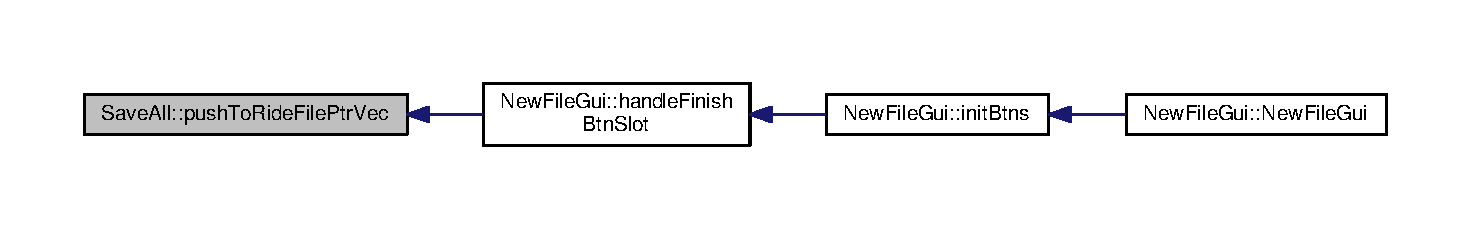
\includegraphics[width=350pt]{namespace_save_all_a2e2571928abdd1b9248fccdba5407df1_icgraph}
\end{center}
\end{figure}


\hypertarget{namespace_save_all_ae4b231ad2bd4a0191668ec36374a39b2}{\index{Save\-All@{Save\-All}!remove\-From\-Ride\-File\-Vec@{remove\-From\-Ride\-File\-Vec}}
\index{remove\-From\-Ride\-File\-Vec@{remove\-From\-Ride\-File\-Vec}!SaveAll@{Save\-All}}
\subsubsection[{remove\-From\-Ride\-File\-Vec}]{\setlength{\rightskip}{0pt plus 5cm}void Save\-All\-::remove\-From\-Ride\-File\-Vec (
\begin{DoxyParamCaption}
\item[{{\bf Ride\-File} $\ast$}]{ride\-File\-Ptr}
\end{DoxyParamCaption}
)}}\label{namespace_save_all_ae4b231ad2bd4a0191668ec36374a39b2}


Definition at line 13 of file Save\-All.\-cpp.



Here is the call graph for this function\-:
\nopagebreak
\begin{figure}[H]
\begin{center}
\leavevmode
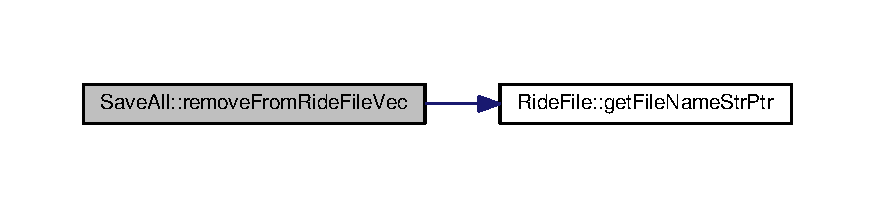
\includegraphics[width=350pt]{namespace_save_all_ae4b231ad2bd4a0191668ec36374a39b2_cgraph}
\end{center}
\end{figure}


\hypertarget{namespace_save_all_ab76b15aa70cf0227fe2ff3c83980d9fc}{\index{Save\-All@{Save\-All}!save@{save}}
\index{save@{save}!SaveAll@{Save\-All}}
\subsubsection[{save}]{\setlength{\rightskip}{0pt plus 5cm}void Save\-All\-::save (
\begin{DoxyParamCaption}
{}
\end{DoxyParamCaption}
)}}\label{namespace_save_all_ab76b15aa70cf0227fe2ff3c83980d9fc}


Definition at line 34 of file Save\-All.\-cpp.



Here is the caller graph for this function\-:
\nopagebreak
\begin{figure}[H]
\begin{center}
\leavevmode
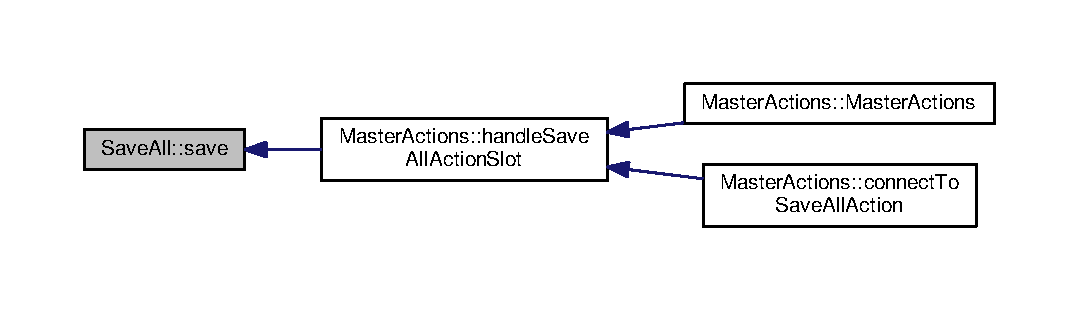
\includegraphics[width=350pt]{namespace_save_all_ab76b15aa70cf0227fe2ff3c83980d9fc_icgraph}
\end{center}
\end{figure}




\subsection{Variable Documentation}
\hypertarget{namespace_save_all_a683cd764fde42d76fc00478beb609f06}{\index{Save\-All@{Save\-All}!ride\-File\-Ptr\-Vec@{ride\-File\-Ptr\-Vec}}
\index{ride\-File\-Ptr\-Vec@{ride\-File\-Ptr\-Vec}!SaveAll@{Save\-All}}
\subsubsection[{ride\-File\-Ptr\-Vec}]{\setlength{\rightskip}{0pt plus 5cm}Q\-Vector$<$ {\bf Ride\-File} $\ast$ $>$ Save\-All\-::ride\-File\-Ptr\-Vec}}\label{namespace_save_all_a683cd764fde42d76fc00478beb609f06}


Definition at line 4 of file Save\-All.\-cpp.


\hypertarget{namespace_tree_item_icon_init}{\section{Tree\-Item\-Icon\-Init Namespace Reference}
\label{namespace_tree_item_icon_init}\index{Tree\-Item\-Icon\-Init@{Tree\-Item\-Icon\-Init}}
}
\subsection*{Functions}
\begin{DoxyCompactItemize}
\item 
void \hyperlink{namespace_tree_item_icon_init_aec158e49ff580b1e64d09b3ec2f12240}{set\-Icon} (Q\-Tree\-Widget\-Item $\ast$child)
\end{DoxyCompactItemize}


\subsection{Function Documentation}
\hypertarget{namespace_tree_item_icon_init_aec158e49ff580b1e64d09b3ec2f12240}{\index{Tree\-Item\-Icon\-Init@{Tree\-Item\-Icon\-Init}!set\-Icon@{set\-Icon}}
\index{set\-Icon@{set\-Icon}!TreeItemIconInit@{Tree\-Item\-Icon\-Init}}
\subsubsection[{set\-Icon}]{\setlength{\rightskip}{0pt plus 5cm}void Tree\-Item\-Icon\-Init\-::set\-Icon (
\begin{DoxyParamCaption}
\item[{Q\-Tree\-Widget\-Item $\ast$}]{child}
\end{DoxyParamCaption}
)}}\label{namespace_tree_item_icon_init_aec158e49ff580b1e64d09b3ec2f12240}


Definition at line 4 of file Tree\-Item\-Icon\-Init.\-cpp.


\hypertarget{namespace_unix_console_text}{\section{Unix\-Console\-Text Namespace Reference}
\label{namespace_unix_console_text}\index{Unix\-Console\-Text@{Unix\-Console\-Text}}
}
\subsection*{Functions}
\begin{DoxyCompactItemize}
\item 
string $\ast$ \hyperlink{namespace_unix_console_text_a08a2fae9dfa6df54be6aa53490d4cee3}{red} (string $\ast$text\-Str\-Ptr)
\item 
string $\ast$ \hyperlink{namespace_unix_console_text_a9b518813d096500605821b99082c0845}{green} (string $\ast$text\-Str\-Ptr)
\item 
string $\ast$ \hyperlink{namespace_unix_console_text_a8ad6638a6663d3b2b6c0d00faec6438e}{yellow} (string $\ast$text\-Str\-Ptr)
\item 
string $\ast$ \hyperlink{namespace_unix_console_text_a32531e5b0b5711cc22e7ca6e09921b67}{blue} (string $\ast$text\-Str\-Ptr)
\item 
string $\ast$ \hyperlink{namespace_unix_console_text_a1c7c0b40a1156e1b513bf9cea29bb72e}{purple} (string $\ast$text\-Str\-Ptr)
\item 
string $\ast$ \hyperlink{namespace_unix_console_text_ab00fc9eacb44b0bafacffb506092bcbe}{cyan} (string $\ast$text\-Str\-Ptr)
\item 
string $\ast$ \hyperlink{namespace_unix_console_text_a464cf03d2963bbbbf988c4660fd8f064}{gray} (string $\ast$text\-Str\-Ptr)
\item 
string $\ast$ \hyperlink{namespace_unix_console_text_af66c25dcb55b26bfdb2e75f36204ad6d}{bold\-Red} (string $\ast$text\-Str\-Ptr)
\item 
string $\ast$ \hyperlink{namespace_unix_console_text_a62cf8804973796c299289560e38ac8b7}{bold\-Green} (string $\ast$text\-Str\-Ptr)
\item 
string $\ast$ \hyperlink{namespace_unix_console_text_aee618445feccbe7ee1192f1b1b8948e7}{bold\-Yellow} (string $\ast$text\-Str\-Ptr)
\item 
string $\ast$ \hyperlink{namespace_unix_console_text_a2d7d1f2ddc072b69b9e85f1f4bf31587}{bold\-Blue} (string $\ast$text\-Str\-Ptr)
\item 
string $\ast$ \hyperlink{namespace_unix_console_text_a2533224f2f47dc725b659479065cd58a}{bold\-Purple} (string $\ast$text\-Str\-Ptr)
\item 
string $\ast$ \hyperlink{namespace_unix_console_text_a3d44cc293cdf1d6ac9a24d7a3e9ab478}{bold\-Cyan} (string $\ast$text\-Str\-Ptr)
\item 
string $\ast$ \hyperlink{namespace_unix_console_text_a1a2cdea64ebb3bbb3f1ee7dae5c055be}{bold\-Gray} (string $\ast$text\-Str\-Ptr)
\item 
string $\ast$ \hyperlink{namespace_unix_console_text_aed8761d2771d1fa621e2f3928e174e1b}{italic\-Red} (string $\ast$text\-Str\-Ptr)
\item 
string $\ast$ \hyperlink{namespace_unix_console_text_a875365603984800fdbf0649fbb23c152}{italic\-Green} (string $\ast$text\-Str\-Ptr)
\item 
string $\ast$ \hyperlink{namespace_unix_console_text_a945b2e41b70a7d47c31c64c25ea10e30}{italic\-Yellow} (string $\ast$text\-Str\-Ptr)
\item 
string $\ast$ \hyperlink{namespace_unix_console_text_aec7de79e37db887a2eb624a2e7c1eb0a}{italic\-Blue} (string $\ast$text\-Str\-Ptr)
\item 
string $\ast$ \hyperlink{namespace_unix_console_text_a7513fc0bb382e2b32a1166a296f90e05}{italic\-Purple} (string $\ast$text\-Str\-Ptr)
\item 
string $\ast$ \hyperlink{namespace_unix_console_text_a82f73127ee8f185170df031d290d9dc6}{italic\-Cyan} (string $\ast$text\-Str\-Ptr)
\item 
string $\ast$ \hyperlink{namespace_unix_console_text_a8fed8b51dfa438319353f7bda5059476}{italic\-Gray} (string $\ast$text\-Str\-Ptr)
\item 
string $\ast$ \hyperlink{namespace_unix_console_text_a10edd17118d2819c67589c1309811140}{underlined\-Red} (string $\ast$text\-Str\-Ptr)
\item 
string $\ast$ \hyperlink{namespace_unix_console_text_a328b088a295baf73367c12177165f4e0}{underlined\-Green} (string $\ast$text\-Str\-Ptr)
\item 
string $\ast$ \hyperlink{namespace_unix_console_text_a205ee04b676b2aebb5ae323839f8de45}{underlined\-Yellow} (string $\ast$text\-Str\-Ptr)
\item 
string $\ast$ \hyperlink{namespace_unix_console_text_a1fe323c83240f6985f0b2c4625cddda3}{underlined\-Blue} (string $\ast$text\-Str\-Ptr)
\item 
string $\ast$ \hyperlink{namespace_unix_console_text_a5870113f7101f12405d9a1ff675a2fc1}{underlined\-Purple} (string $\ast$text\-Str\-Ptr)
\item 
string $\ast$ \hyperlink{namespace_unix_console_text_ad29ff223c9f8745e6ed7e0994b36a629}{underlined\-Cyan} (string $\ast$text\-Str\-Ptr)
\item 
string $\ast$ \hyperlink{namespace_unix_console_text_a67d5c2e42c36ff8ae618643a1e9e0523}{underlined\-Gray} (string $\ast$text\-Str\-Ptr)
\end{DoxyCompactItemize}


\subsection{Function Documentation}
\hypertarget{namespace_unix_console_text_a32531e5b0b5711cc22e7ca6e09921b67}{\index{Unix\-Console\-Text@{Unix\-Console\-Text}!blue@{blue}}
\index{blue@{blue}!UnixConsoleText@{Unix\-Console\-Text}}
\subsubsection[{blue}]{\setlength{\rightskip}{0pt plus 5cm}string $\ast$ Unix\-Console\-Text\-::blue (
\begin{DoxyParamCaption}
\item[{string $\ast$}]{text\-Str\-Ptr}
\end{DoxyParamCaption}
)}}\label{namespace_unix_console_text_a32531e5b0b5711cc22e7ca6e09921b67}
Method to return blue text\-Str\-Ptr.


\begin{DoxyParams}{Parameters}
{\em text\-Str\-Ptr} & text\-Str\-Ptr to be printed blue. \\
\hline
\end{DoxyParams}
\begin{DoxyReturn}{Returns}
Blue text\-Str\-Ptr. 
\end{DoxyReturn}


Definition at line 23 of file Unix\-Console\-Text.\-cpp.

\hypertarget{namespace_unix_console_text_a2d7d1f2ddc072b69b9e85f1f4bf31587}{\index{Unix\-Console\-Text@{Unix\-Console\-Text}!bold\-Blue@{bold\-Blue}}
\index{bold\-Blue@{bold\-Blue}!UnixConsoleText@{Unix\-Console\-Text}}
\subsubsection[{bold\-Blue}]{\setlength{\rightskip}{0pt plus 5cm}string $\ast$ Unix\-Console\-Text\-::bold\-Blue (
\begin{DoxyParamCaption}
\item[{string $\ast$}]{text\-Str\-Ptr}
\end{DoxyParamCaption}
)}}\label{namespace_unix_console_text_a2d7d1f2ddc072b69b9e85f1f4bf31587}
Method to return bold blue text\-Str\-Ptr.


\begin{DoxyParams}{Parameters}
{\em text\-Str\-Ptr} & text\-Str\-Ptr to be printed bold blue. \\
\hline
\end{DoxyParams}
\begin{DoxyReturn}{Returns}
Bold blue text\-Str\-Ptr. 
\end{DoxyReturn}


Definition at line 69 of file Unix\-Console\-Text.\-cpp.

\hypertarget{namespace_unix_console_text_a3d44cc293cdf1d6ac9a24d7a3e9ab478}{\index{Unix\-Console\-Text@{Unix\-Console\-Text}!bold\-Cyan@{bold\-Cyan}}
\index{bold\-Cyan@{bold\-Cyan}!UnixConsoleText@{Unix\-Console\-Text}}
\subsubsection[{bold\-Cyan}]{\setlength{\rightskip}{0pt plus 5cm}string $\ast$ Unix\-Console\-Text\-::bold\-Cyan (
\begin{DoxyParamCaption}
\item[{string $\ast$}]{text\-Str\-Ptr}
\end{DoxyParamCaption}
)}}\label{namespace_unix_console_text_a3d44cc293cdf1d6ac9a24d7a3e9ab478}
Method to return bold cyan text\-Str\-Ptr.


\begin{DoxyParams}{Parameters}
{\em text\-Str\-Ptr} & text\-Str\-Ptr to be printed bold cyan. \\
\hline
\end{DoxyParams}
\begin{DoxyReturn}{Returns}
Bold cyan text\-Str\-Ptr. 
\end{DoxyReturn}


Definition at line 81 of file Unix\-Console\-Text.\-cpp.

\hypertarget{namespace_unix_console_text_a1a2cdea64ebb3bbb3f1ee7dae5c055be}{\index{Unix\-Console\-Text@{Unix\-Console\-Text}!bold\-Gray@{bold\-Gray}}
\index{bold\-Gray@{bold\-Gray}!UnixConsoleText@{Unix\-Console\-Text}}
\subsubsection[{bold\-Gray}]{\setlength{\rightskip}{0pt plus 5cm}string $\ast$ Unix\-Console\-Text\-::bold\-Gray (
\begin{DoxyParamCaption}
\item[{string $\ast$}]{text\-Str\-Ptr}
\end{DoxyParamCaption}
)}}\label{namespace_unix_console_text_a1a2cdea64ebb3bbb3f1ee7dae5c055be}
Method to return bold gray text\-Str\-Ptr.


\begin{DoxyParams}{Parameters}
{\em text\-Str\-Ptr} & text\-Str\-Ptr to be printed bold gray. \\
\hline
\end{DoxyParams}
\begin{DoxyReturn}{Returns}
Bold gray text\-Str\-Ptr. 
\end{DoxyReturn}


Definition at line 87 of file Unix\-Console\-Text.\-cpp.

\hypertarget{namespace_unix_console_text_a62cf8804973796c299289560e38ac8b7}{\index{Unix\-Console\-Text@{Unix\-Console\-Text}!bold\-Green@{bold\-Green}}
\index{bold\-Green@{bold\-Green}!UnixConsoleText@{Unix\-Console\-Text}}
\subsubsection[{bold\-Green}]{\setlength{\rightskip}{0pt plus 5cm}string $\ast$ Unix\-Console\-Text\-::bold\-Green (
\begin{DoxyParamCaption}
\item[{string $\ast$}]{text\-Str\-Ptr}
\end{DoxyParamCaption}
)}}\label{namespace_unix_console_text_a62cf8804973796c299289560e38ac8b7}
Method to return bold green text\-Str\-Ptr.


\begin{DoxyParams}{Parameters}
{\em text\-Str\-Ptr} & text\-Str\-Ptr to be printed bold green. \\
\hline
\end{DoxyParams}
\begin{DoxyReturn}{Returns}
Bold green text\-Str\-Ptr. 
\end{DoxyReturn}


Definition at line 57 of file Unix\-Console\-Text.\-cpp.

\hypertarget{namespace_unix_console_text_a2533224f2f47dc725b659479065cd58a}{\index{Unix\-Console\-Text@{Unix\-Console\-Text}!bold\-Purple@{bold\-Purple}}
\index{bold\-Purple@{bold\-Purple}!UnixConsoleText@{Unix\-Console\-Text}}
\subsubsection[{bold\-Purple}]{\setlength{\rightskip}{0pt plus 5cm}string $\ast$ Unix\-Console\-Text\-::bold\-Purple (
\begin{DoxyParamCaption}
\item[{string $\ast$}]{text\-Str\-Ptr}
\end{DoxyParamCaption}
)}}\label{namespace_unix_console_text_a2533224f2f47dc725b659479065cd58a}
Method to return bold purple text\-Str\-Ptr.


\begin{DoxyParams}{Parameters}
{\em text\-Str\-Ptr} & text\-Str\-Ptr to be printed bold purple. \\
\hline
\end{DoxyParams}
\begin{DoxyReturn}{Returns}
Bold purple text\-Str\-Ptr. 
\end{DoxyReturn}


Definition at line 75 of file Unix\-Console\-Text.\-cpp.

\hypertarget{namespace_unix_console_text_af66c25dcb55b26bfdb2e75f36204ad6d}{\index{Unix\-Console\-Text@{Unix\-Console\-Text}!bold\-Red@{bold\-Red}}
\index{bold\-Red@{bold\-Red}!UnixConsoleText@{Unix\-Console\-Text}}
\subsubsection[{bold\-Red}]{\setlength{\rightskip}{0pt plus 5cm}string $\ast$ Unix\-Console\-Text\-::bold\-Red (
\begin{DoxyParamCaption}
\item[{string $\ast$}]{text\-Str\-Ptr}
\end{DoxyParamCaption}
)}}\label{namespace_unix_console_text_af66c25dcb55b26bfdb2e75f36204ad6d}
Method to return bold red text\-Str\-Ptr.


\begin{DoxyParams}{Parameters}
{\em text\-Str\-Ptr} & text\-Str\-Ptr to be printed bold red. \\
\hline
\end{DoxyParams}
\begin{DoxyReturn}{Returns}
Bold red text\-Str\-Ptr. 
\end{DoxyReturn}


Definition at line 51 of file Unix\-Console\-Text.\-cpp.

\hypertarget{namespace_unix_console_text_aee618445feccbe7ee1192f1b1b8948e7}{\index{Unix\-Console\-Text@{Unix\-Console\-Text}!bold\-Yellow@{bold\-Yellow}}
\index{bold\-Yellow@{bold\-Yellow}!UnixConsoleText@{Unix\-Console\-Text}}
\subsubsection[{bold\-Yellow}]{\setlength{\rightskip}{0pt plus 5cm}string $\ast$ Unix\-Console\-Text\-::bold\-Yellow (
\begin{DoxyParamCaption}
\item[{string $\ast$}]{text\-Str\-Ptr}
\end{DoxyParamCaption}
)}}\label{namespace_unix_console_text_aee618445feccbe7ee1192f1b1b8948e7}
Method to return bold yellow text\-Str\-Ptr.


\begin{DoxyParams}{Parameters}
{\em text\-Str\-Ptr} & text\-Str\-Ptr to be printed bold yellow. \\
\hline
\end{DoxyParams}
\begin{DoxyReturn}{Returns}
Bold yellow text\-Str\-Ptr. 
\end{DoxyReturn}


Definition at line 63 of file Unix\-Console\-Text.\-cpp.

\hypertarget{namespace_unix_console_text_ab00fc9eacb44b0bafacffb506092bcbe}{\index{Unix\-Console\-Text@{Unix\-Console\-Text}!cyan@{cyan}}
\index{cyan@{cyan}!UnixConsoleText@{Unix\-Console\-Text}}
\subsubsection[{cyan}]{\setlength{\rightskip}{0pt plus 5cm}string $\ast$ Unix\-Console\-Text\-::cyan (
\begin{DoxyParamCaption}
\item[{string $\ast$}]{text\-Str\-Ptr}
\end{DoxyParamCaption}
)}}\label{namespace_unix_console_text_ab00fc9eacb44b0bafacffb506092bcbe}
Method to return cyan text\-Str\-Ptr.


\begin{DoxyParams}{Parameters}
{\em text\-Str\-Ptr} & text\-Str\-Ptr to be printed cyan. \\
\hline
\end{DoxyParams}
\begin{DoxyReturn}{Returns}
Cyan text\-Str\-Ptr. 
\end{DoxyReturn}


Definition at line 35 of file Unix\-Console\-Text.\-cpp.

\hypertarget{namespace_unix_console_text_a464cf03d2963bbbbf988c4660fd8f064}{\index{Unix\-Console\-Text@{Unix\-Console\-Text}!gray@{gray}}
\index{gray@{gray}!UnixConsoleText@{Unix\-Console\-Text}}
\subsubsection[{gray}]{\setlength{\rightskip}{0pt plus 5cm}string $\ast$ Unix\-Console\-Text\-::gray (
\begin{DoxyParamCaption}
\item[{string $\ast$}]{text\-Str\-Ptr}
\end{DoxyParamCaption}
)}}\label{namespace_unix_console_text_a464cf03d2963bbbbf988c4660fd8f064}
Method to return gray text\-Str\-Ptr.


\begin{DoxyParams}{Parameters}
{\em text\-Str\-Ptr} & text\-Str\-Ptr to be printed gray. \\
\hline
\end{DoxyParams}
\begin{DoxyReturn}{Returns}
Gray text\-Str\-Ptr. 
\end{DoxyReturn}


Definition at line 41 of file Unix\-Console\-Text.\-cpp.

\hypertarget{namespace_unix_console_text_a9b518813d096500605821b99082c0845}{\index{Unix\-Console\-Text@{Unix\-Console\-Text}!green@{green}}
\index{green@{green}!UnixConsoleText@{Unix\-Console\-Text}}
\subsubsection[{green}]{\setlength{\rightskip}{0pt plus 5cm}string $\ast$ Unix\-Console\-Text\-::green (
\begin{DoxyParamCaption}
\item[{string $\ast$}]{text\-Str\-Ptr}
\end{DoxyParamCaption}
)}}\label{namespace_unix_console_text_a9b518813d096500605821b99082c0845}
Method to return green text\-Str\-Ptr.


\begin{DoxyParams}{Parameters}
{\em text\-Str\-Ptr} & text\-Str\-Ptr to be printed green. \\
\hline
\end{DoxyParams}
\begin{DoxyReturn}{Returns}
Green text\-Str\-Ptr. 
\end{DoxyReturn}


Definition at line 11 of file Unix\-Console\-Text.\-cpp.

\hypertarget{namespace_unix_console_text_aec7de79e37db887a2eb624a2e7c1eb0a}{\index{Unix\-Console\-Text@{Unix\-Console\-Text}!italic\-Blue@{italic\-Blue}}
\index{italic\-Blue@{italic\-Blue}!UnixConsoleText@{Unix\-Console\-Text}}
\subsubsection[{italic\-Blue}]{\setlength{\rightskip}{0pt plus 5cm}string $\ast$ Unix\-Console\-Text\-::italic\-Blue (
\begin{DoxyParamCaption}
\item[{string $\ast$}]{text\-Str\-Ptr}
\end{DoxyParamCaption}
)}}\label{namespace_unix_console_text_aec7de79e37db887a2eb624a2e7c1eb0a}
Method to return italic blue text\-Str\-Ptr.


\begin{DoxyParams}{Parameters}
{\em text\-Str\-Ptr} & text\-Str\-Ptr to be printed italic blue. \\
\hline
\end{DoxyParams}
\begin{DoxyReturn}{Returns}
Italic blue text\-Str\-Ptr. 
\end{DoxyReturn}


Definition at line 111 of file Unix\-Console\-Text.\-cpp.

\hypertarget{namespace_unix_console_text_a82f73127ee8f185170df031d290d9dc6}{\index{Unix\-Console\-Text@{Unix\-Console\-Text}!italic\-Cyan@{italic\-Cyan}}
\index{italic\-Cyan@{italic\-Cyan}!UnixConsoleText@{Unix\-Console\-Text}}
\subsubsection[{italic\-Cyan}]{\setlength{\rightskip}{0pt plus 5cm}string $\ast$ Unix\-Console\-Text\-::italic\-Cyan (
\begin{DoxyParamCaption}
\item[{string $\ast$}]{text\-Str\-Ptr}
\end{DoxyParamCaption}
)}}\label{namespace_unix_console_text_a82f73127ee8f185170df031d290d9dc6}
Method to return italic cyan text\-Str\-Ptr.


\begin{DoxyParams}{Parameters}
{\em text\-Str\-Ptr} & text\-Str\-Ptr to be printed italic cyan. \\
\hline
\end{DoxyParams}
\begin{DoxyReturn}{Returns}
Italic cyan text\-Str\-Ptr. 
\end{DoxyReturn}


Definition at line 123 of file Unix\-Console\-Text.\-cpp.

\hypertarget{namespace_unix_console_text_a8fed8b51dfa438319353f7bda5059476}{\index{Unix\-Console\-Text@{Unix\-Console\-Text}!italic\-Gray@{italic\-Gray}}
\index{italic\-Gray@{italic\-Gray}!UnixConsoleText@{Unix\-Console\-Text}}
\subsubsection[{italic\-Gray}]{\setlength{\rightskip}{0pt plus 5cm}string $\ast$ Unix\-Console\-Text\-::italic\-Gray (
\begin{DoxyParamCaption}
\item[{string $\ast$}]{text\-Str\-Ptr}
\end{DoxyParamCaption}
)}}\label{namespace_unix_console_text_a8fed8b51dfa438319353f7bda5059476}
Method to return italic gray text\-Str\-Ptr.


\begin{DoxyParams}{Parameters}
{\em text\-Str\-Ptr} & text\-Str\-Ptr to be printed italic gray. \\
\hline
\end{DoxyParams}
\begin{DoxyReturn}{Returns}
Italic gray text\-Str\-Ptr. 
\end{DoxyReturn}


Definition at line 129 of file Unix\-Console\-Text.\-cpp.

\hypertarget{namespace_unix_console_text_a875365603984800fdbf0649fbb23c152}{\index{Unix\-Console\-Text@{Unix\-Console\-Text}!italic\-Green@{italic\-Green}}
\index{italic\-Green@{italic\-Green}!UnixConsoleText@{Unix\-Console\-Text}}
\subsubsection[{italic\-Green}]{\setlength{\rightskip}{0pt plus 5cm}string $\ast$ Unix\-Console\-Text\-::italic\-Green (
\begin{DoxyParamCaption}
\item[{string $\ast$}]{text\-Str\-Ptr}
\end{DoxyParamCaption}
)}}\label{namespace_unix_console_text_a875365603984800fdbf0649fbb23c152}
Method to return italic green text\-Str\-Ptr.


\begin{DoxyParams}{Parameters}
{\em text\-Str\-Ptr} & text\-Str\-Ptr to be printed italic green. \\
\hline
\end{DoxyParams}
\begin{DoxyReturn}{Returns}
Italic green text\-Str\-Ptr. 
\end{DoxyReturn}


Definition at line 99 of file Unix\-Console\-Text.\-cpp.

\hypertarget{namespace_unix_console_text_a7513fc0bb382e2b32a1166a296f90e05}{\index{Unix\-Console\-Text@{Unix\-Console\-Text}!italic\-Purple@{italic\-Purple}}
\index{italic\-Purple@{italic\-Purple}!UnixConsoleText@{Unix\-Console\-Text}}
\subsubsection[{italic\-Purple}]{\setlength{\rightskip}{0pt plus 5cm}string $\ast$ Unix\-Console\-Text\-::italic\-Purple (
\begin{DoxyParamCaption}
\item[{string $\ast$}]{text\-Str\-Ptr}
\end{DoxyParamCaption}
)}}\label{namespace_unix_console_text_a7513fc0bb382e2b32a1166a296f90e05}
Method to return italic purple text\-Str\-Ptr.


\begin{DoxyParams}{Parameters}
{\em text\-Str\-Ptr} & text\-Str\-Ptr to be printed italic purple. \\
\hline
\end{DoxyParams}
\begin{DoxyReturn}{Returns}
Italic purple text\-Str\-Ptr. 
\end{DoxyReturn}


Definition at line 117 of file Unix\-Console\-Text.\-cpp.

\hypertarget{namespace_unix_console_text_aed8761d2771d1fa621e2f3928e174e1b}{\index{Unix\-Console\-Text@{Unix\-Console\-Text}!italic\-Red@{italic\-Red}}
\index{italic\-Red@{italic\-Red}!UnixConsoleText@{Unix\-Console\-Text}}
\subsubsection[{italic\-Red}]{\setlength{\rightskip}{0pt plus 5cm}string $\ast$ Unix\-Console\-Text\-::italic\-Red (
\begin{DoxyParamCaption}
\item[{string $\ast$}]{text\-Str\-Ptr}
\end{DoxyParamCaption}
)}}\label{namespace_unix_console_text_aed8761d2771d1fa621e2f3928e174e1b}
Method to return italic red text\-Str\-Ptr.


\begin{DoxyParams}{Parameters}
{\em text\-Str\-Ptr} & text\-Str\-Ptr to be printed italic red. \\
\hline
\end{DoxyParams}
\begin{DoxyReturn}{Returns}
Italic red text\-Str\-Ptr. 
\end{DoxyReturn}


Definition at line 93 of file Unix\-Console\-Text.\-cpp.

\hypertarget{namespace_unix_console_text_a945b2e41b70a7d47c31c64c25ea10e30}{\index{Unix\-Console\-Text@{Unix\-Console\-Text}!italic\-Yellow@{italic\-Yellow}}
\index{italic\-Yellow@{italic\-Yellow}!UnixConsoleText@{Unix\-Console\-Text}}
\subsubsection[{italic\-Yellow}]{\setlength{\rightskip}{0pt plus 5cm}string $\ast$ Unix\-Console\-Text\-::italic\-Yellow (
\begin{DoxyParamCaption}
\item[{string $\ast$}]{text\-Str\-Ptr}
\end{DoxyParamCaption}
)}}\label{namespace_unix_console_text_a945b2e41b70a7d47c31c64c25ea10e30}
Method to return italic yellow text\-Str\-Ptr.


\begin{DoxyParams}{Parameters}
{\em text\-Str\-Ptr} & text\-Str\-Ptr to be printed italic yellow. \\
\hline
\end{DoxyParams}
\begin{DoxyReturn}{Returns}
Italic yellow text\-Str\-Ptr. 
\end{DoxyReturn}


Definition at line 105 of file Unix\-Console\-Text.\-cpp.

\hypertarget{namespace_unix_console_text_a1c7c0b40a1156e1b513bf9cea29bb72e}{\index{Unix\-Console\-Text@{Unix\-Console\-Text}!purple@{purple}}
\index{purple@{purple}!UnixConsoleText@{Unix\-Console\-Text}}
\subsubsection[{purple}]{\setlength{\rightskip}{0pt plus 5cm}string $\ast$ Unix\-Console\-Text\-::purple (
\begin{DoxyParamCaption}
\item[{string $\ast$}]{text\-Str\-Ptr}
\end{DoxyParamCaption}
)}}\label{namespace_unix_console_text_a1c7c0b40a1156e1b513bf9cea29bb72e}
Method to return purple text\-Str\-Ptr.


\begin{DoxyParams}{Parameters}
{\em text\-Str\-Ptr} & text\-Str\-Ptr to be printed purple. \\
\hline
\end{DoxyParams}
\begin{DoxyReturn}{Returns}
Purple text\-Str\-Ptr. 
\end{DoxyReturn}


Definition at line 29 of file Unix\-Console\-Text.\-cpp.

\hypertarget{namespace_unix_console_text_a08a2fae9dfa6df54be6aa53490d4cee3}{\index{Unix\-Console\-Text@{Unix\-Console\-Text}!red@{red}}
\index{red@{red}!UnixConsoleText@{Unix\-Console\-Text}}
\subsubsection[{red}]{\setlength{\rightskip}{0pt plus 5cm}string $\ast$ Unix\-Console\-Text\-::red (
\begin{DoxyParamCaption}
\item[{string $\ast$}]{text\-Str\-Ptr}
\end{DoxyParamCaption}
)}}\label{namespace_unix_console_text_a08a2fae9dfa6df54be6aa53490d4cee3}
Method to return red text\-Str\-Ptr.


\begin{DoxyParams}{Parameters}
{\em text\-Str\-Ptr} & text\-Str\-Ptr to be printed red. \\
\hline
\end{DoxyParams}
\begin{DoxyReturn}{Returns}
Red text\-Str\-Ptr. 
\end{DoxyReturn}


Definition at line 4 of file Unix\-Console\-Text.\-cpp.

\hypertarget{namespace_unix_console_text_a1fe323c83240f6985f0b2c4625cddda3}{\index{Unix\-Console\-Text@{Unix\-Console\-Text}!underlined\-Blue@{underlined\-Blue}}
\index{underlined\-Blue@{underlined\-Blue}!UnixConsoleText@{Unix\-Console\-Text}}
\subsubsection[{underlined\-Blue}]{\setlength{\rightskip}{0pt plus 5cm}string $\ast$ Unix\-Console\-Text\-::underlined\-Blue (
\begin{DoxyParamCaption}
\item[{string $\ast$}]{text\-Str\-Ptr}
\end{DoxyParamCaption}
)}}\label{namespace_unix_console_text_a1fe323c83240f6985f0b2c4625cddda3}
Method to return underlined blue text\-Str\-Ptr.


\begin{DoxyParams}{Parameters}
{\em text\-Str\-Ptr} & text\-Str\-Ptr to be printed underlined blue. \\
\hline
\end{DoxyParams}
\begin{DoxyReturn}{Returns}
Underlined blue text\-Str\-Ptr. 
\end{DoxyReturn}


Definition at line 156 of file Unix\-Console\-Text.\-cpp.

\hypertarget{namespace_unix_console_text_ad29ff223c9f8745e6ed7e0994b36a629}{\index{Unix\-Console\-Text@{Unix\-Console\-Text}!underlined\-Cyan@{underlined\-Cyan}}
\index{underlined\-Cyan@{underlined\-Cyan}!UnixConsoleText@{Unix\-Console\-Text}}
\subsubsection[{underlined\-Cyan}]{\setlength{\rightskip}{0pt plus 5cm}string $\ast$ Unix\-Console\-Text\-::underlined\-Cyan (
\begin{DoxyParamCaption}
\item[{string $\ast$}]{text\-Str\-Ptr}
\end{DoxyParamCaption}
)}}\label{namespace_unix_console_text_ad29ff223c9f8745e6ed7e0994b36a629}
Method to return underlined cyan text\-Str\-Ptr.


\begin{DoxyParams}{Parameters}
{\em text\-Str\-Ptr} & text\-Str\-Ptr to be printed underlined cyan. \\
\hline
\end{DoxyParams}
\begin{DoxyReturn}{Returns}
Underlined cyan text\-Str\-Ptr. 
\end{DoxyReturn}


Definition at line 168 of file Unix\-Console\-Text.\-cpp.

\hypertarget{namespace_unix_console_text_a67d5c2e42c36ff8ae618643a1e9e0523}{\index{Unix\-Console\-Text@{Unix\-Console\-Text}!underlined\-Gray@{underlined\-Gray}}
\index{underlined\-Gray@{underlined\-Gray}!UnixConsoleText@{Unix\-Console\-Text}}
\subsubsection[{underlined\-Gray}]{\setlength{\rightskip}{0pt plus 5cm}string $\ast$ Unix\-Console\-Text\-::underlined\-Gray (
\begin{DoxyParamCaption}
\item[{string $\ast$}]{text\-Str\-Ptr}
\end{DoxyParamCaption}
)}}\label{namespace_unix_console_text_a67d5c2e42c36ff8ae618643a1e9e0523}
Method to return underlined gray text\-Str\-Ptr.


\begin{DoxyParams}{Parameters}
{\em text\-Str\-Ptr} & text\-Str\-Ptr to be printed underlined gray. \\
\hline
\end{DoxyParams}
\begin{DoxyReturn}{Returns}
Underlined gray text\-Str\-Ptr. 
\end{DoxyReturn}


Definition at line 174 of file Unix\-Console\-Text.\-cpp.

\hypertarget{namespace_unix_console_text_a328b088a295baf73367c12177165f4e0}{\index{Unix\-Console\-Text@{Unix\-Console\-Text}!underlined\-Green@{underlined\-Green}}
\index{underlined\-Green@{underlined\-Green}!UnixConsoleText@{Unix\-Console\-Text}}
\subsubsection[{underlined\-Green}]{\setlength{\rightskip}{0pt plus 5cm}string $\ast$ Unix\-Console\-Text\-::underlined\-Green (
\begin{DoxyParamCaption}
\item[{string $\ast$}]{text\-Str\-Ptr}
\end{DoxyParamCaption}
)}}\label{namespace_unix_console_text_a328b088a295baf73367c12177165f4e0}
Method to return underlined green text\-Str\-Ptr.


\begin{DoxyParams}{Parameters}
{\em text\-Str\-Ptr} & text\-Str\-Ptr to be printed underlined green. \\
\hline
\end{DoxyParams}
\begin{DoxyReturn}{Returns}
Underlined green text\-Str\-Ptr. 
\end{DoxyReturn}


Definition at line 144 of file Unix\-Console\-Text.\-cpp.

\hypertarget{namespace_unix_console_text_a5870113f7101f12405d9a1ff675a2fc1}{\index{Unix\-Console\-Text@{Unix\-Console\-Text}!underlined\-Purple@{underlined\-Purple}}
\index{underlined\-Purple@{underlined\-Purple}!UnixConsoleText@{Unix\-Console\-Text}}
\subsubsection[{underlined\-Purple}]{\setlength{\rightskip}{0pt plus 5cm}string $\ast$ Unix\-Console\-Text\-::underlined\-Purple (
\begin{DoxyParamCaption}
\item[{string $\ast$}]{text\-Str\-Ptr}
\end{DoxyParamCaption}
)}}\label{namespace_unix_console_text_a5870113f7101f12405d9a1ff675a2fc1}
Method to return underlined purple text\-Str\-Ptr.


\begin{DoxyParams}{Parameters}
{\em text\-Str\-Ptr} & text\-Str\-Ptr to be printed underlined purple. \\
\hline
\end{DoxyParams}
\begin{DoxyReturn}{Returns}
Underlined purple text\-Str\-Ptr. 
\end{DoxyReturn}


Definition at line 162 of file Unix\-Console\-Text.\-cpp.

\hypertarget{namespace_unix_console_text_a10edd17118d2819c67589c1309811140}{\index{Unix\-Console\-Text@{Unix\-Console\-Text}!underlined\-Red@{underlined\-Red}}
\index{underlined\-Red@{underlined\-Red}!UnixConsoleText@{Unix\-Console\-Text}}
\subsubsection[{underlined\-Red}]{\setlength{\rightskip}{0pt plus 5cm}string $\ast$ Unix\-Console\-Text\-::underlined\-Red (
\begin{DoxyParamCaption}
\item[{string $\ast$}]{text\-Str\-Ptr}
\end{DoxyParamCaption}
)}}\label{namespace_unix_console_text_a10edd17118d2819c67589c1309811140}
Method to return underlined red text\-Str\-Ptr.


\begin{DoxyParams}{Parameters}
{\em text\-Str\-Ptr} & text\-Str\-Ptr to be printed underlined red. \\
\hline
\end{DoxyParams}
\begin{DoxyReturn}{Returns}
Underlined red text\-Str\-Ptr. 
\end{DoxyReturn}


Definition at line 138 of file Unix\-Console\-Text.\-cpp.

\hypertarget{namespace_unix_console_text_a205ee04b676b2aebb5ae323839f8de45}{\index{Unix\-Console\-Text@{Unix\-Console\-Text}!underlined\-Yellow@{underlined\-Yellow}}
\index{underlined\-Yellow@{underlined\-Yellow}!UnixConsoleText@{Unix\-Console\-Text}}
\subsubsection[{underlined\-Yellow}]{\setlength{\rightskip}{0pt plus 5cm}string $\ast$ Unix\-Console\-Text\-::underlined\-Yellow (
\begin{DoxyParamCaption}
\item[{string $\ast$}]{text\-Str\-Ptr}
\end{DoxyParamCaption}
)}}\label{namespace_unix_console_text_a205ee04b676b2aebb5ae323839f8de45}
Method to return underlined yellow text\-Str\-Ptr.


\begin{DoxyParams}{Parameters}
{\em text\-Str\-Ptr} & text\-Str\-Ptr to be printed underlined yellow. \\
\hline
\end{DoxyParams}
\begin{DoxyReturn}{Returns}
Underlined yellow text\-Str\-Ptr. 
\end{DoxyReturn}


Definition at line 150 of file Unix\-Console\-Text.\-cpp.

\hypertarget{namespace_unix_console_text_a8ad6638a6663d3b2b6c0d00faec6438e}{\index{Unix\-Console\-Text@{Unix\-Console\-Text}!yellow@{yellow}}
\index{yellow@{yellow}!UnixConsoleText@{Unix\-Console\-Text}}
\subsubsection[{yellow}]{\setlength{\rightskip}{0pt plus 5cm}string $\ast$ Unix\-Console\-Text\-::yellow (
\begin{DoxyParamCaption}
\item[{string $\ast$}]{text\-Str\-Ptr}
\end{DoxyParamCaption}
)}}\label{namespace_unix_console_text_a8ad6638a6663d3b2b6c0d00faec6438e}
Method to return yellow text\-Str\-Ptr.


\begin{DoxyParams}{Parameters}
{\em text\-Str\-Ptr} & text\-Str\-Ptr to be printed yellow. \\
\hline
\end{DoxyParams}
\begin{DoxyReturn}{Returns}
Yellow text\-Str\-Ptr. 
\end{DoxyReturn}


Definition at line 17 of file Unix\-Console\-Text.\-cpp.


\hypertarget{namespace_windows_console_text}{\section{Windows\-Console\-Text Namespace Reference}
\label{namespace_windows_console_text}\index{Windows\-Console\-Text@{Windows\-Console\-Text}}
}
\subsection*{Functions}
\begin{DoxyCompactItemize}
\item 
string $\ast$ \hyperlink{namespace_windows_console_text_a0b3bd4d8c412a8208762be06cf2c7ddd}{red} (string $\ast$text\-Str\-Ptr)
\item 
string $\ast$ \hyperlink{namespace_windows_console_text_a3b5e5879c4a73adde641f69b9c5c692b}{green} (string $\ast$text\-Str\-Ptr)
\item 
string $\ast$ \hyperlink{namespace_windows_console_text_a13969e6a4cdad5b49196fb843585fef2}{yellow} (string $\ast$text\-Str\-Ptr)
\item 
string $\ast$ \hyperlink{namespace_windows_console_text_a7bbbf356662bad883f5e777a14c89ed8}{blue} (string $\ast$text\-Str\-Ptr)
\item 
string $\ast$ \hyperlink{namespace_windows_console_text_aff0abcf384e233f425332c77a07a45ac}{purple} (string $\ast$text\-Str\-Ptr)
\item 
string $\ast$ \hyperlink{namespace_windows_console_text_a4b1c94cd1e4282defb9baa7bf368fc64}{cyan} (string $\ast$text\-Str\-Ptr)
\item 
string $\ast$ \hyperlink{namespace_windows_console_text_a71de428c5c1012768568a554909ce21e}{gray} (string $\ast$text\-Str\-Ptr)
\item 
string $\ast$ \hyperlink{namespace_windows_console_text_a4e7b50f0fec313c7e650eb0a70012c3e}{bold\-Red} (string $\ast$text\-Str\-Ptr)
\item 
string $\ast$ \hyperlink{namespace_windows_console_text_aaec121e923f7ea5e3b7665c783044d1e}{bold\-Green} (string $\ast$text\-Str\-Ptr)
\item 
string $\ast$ \hyperlink{namespace_windows_console_text_ab12845c763ce135aaa1e45efb61f49d9}{bold\-Yellow} (string $\ast$text\-Str\-Ptr)
\item 
string $\ast$ \hyperlink{namespace_windows_console_text_a37e1e314abe02a10b3d55a66ba74c031}{bold\-Blue} (string $\ast$text\-Str\-Ptr)
\item 
string $\ast$ \hyperlink{namespace_windows_console_text_a0157e7ea4c376fd86f05764d8c1242a1}{bold\-Purple} (string $\ast$text\-Str\-Ptr)
\item 
string $\ast$ \hyperlink{namespace_windows_console_text_ad663bdad1383d48b6202cbe2d22f7c2e}{bold\-Cyan} (string $\ast$text\-Str\-Ptr)
\item 
string $\ast$ \hyperlink{namespace_windows_console_text_ae4eabe670d07ffade22db0e87aee5249}{bold\-Gray} (string $\ast$text\-Str\-Ptr)
\item 
string $\ast$ \hyperlink{namespace_windows_console_text_a71db4269f200b021de61913d2b7903f2}{italic\-Red} (string $\ast$text\-Str\-Ptr)
\item 
string $\ast$ \hyperlink{namespace_windows_console_text_ae8a44033301cf0b159f890bb17e9ade0}{italic\-Green} (string $\ast$text\-Str\-Ptr)
\item 
string $\ast$ \hyperlink{namespace_windows_console_text_af7505c56ac71c073a30f9c7497ea5dd8}{italic\-Yellow} (string $\ast$text\-Str\-Ptr)
\item 
string $\ast$ \hyperlink{namespace_windows_console_text_a43e272994e8370c6cc1e8289872cc3f1}{italic\-Blue} (string $\ast$text\-Str\-Ptr)
\item 
string $\ast$ \hyperlink{namespace_windows_console_text_a2ccdabfc1d8ffe166c063c039bd0a674}{italic\-Purple} (string $\ast$text\-Str\-Ptr)
\item 
string $\ast$ \hyperlink{namespace_windows_console_text_adeb5de271a3357ae4e3cca4faa7a2f1c}{italic\-Cyan} (string $\ast$text\-Str\-Ptr)
\item 
string $\ast$ \hyperlink{namespace_windows_console_text_a4263561267b05b8eb062d4291ad48156}{italic\-Gray} (string $\ast$text\-Str\-Ptr)
\item 
string $\ast$ \hyperlink{namespace_windows_console_text_a58b2e71e3c82e6a5fd9470d94fd0e339}{underlined\-Red} (string $\ast$text\-Str\-Ptr)
\item 
string $\ast$ \hyperlink{namespace_windows_console_text_ae2d3c6f156dfd20fbcaf002f60c3063a}{underlined\-Green} (string $\ast$text\-Str\-Ptr)
\item 
string $\ast$ \hyperlink{namespace_windows_console_text_ae57c84df042a9ea941f83edd16e3c24a}{underlined\-Yellow} (string $\ast$text\-Str\-Ptr)
\item 
string $\ast$ \hyperlink{namespace_windows_console_text_a318921dc20bbc206b4c20f5c20fcd01f}{underlined\-Blue} (string $\ast$text\-Str\-Ptr)
\item 
string $\ast$ \hyperlink{namespace_windows_console_text_adddcdb4ed3b84b741d98d0e1ea2e4921}{underlined\-Purple} (string $\ast$text\-Str\-Ptr)
\item 
string $\ast$ \hyperlink{namespace_windows_console_text_a20c98475a28eb10d06e9dd2a6259ce5b}{underlined\-Cyan} (string $\ast$text\-Str\-Ptr)
\item 
string $\ast$ \hyperlink{namespace_windows_console_text_acc55d1a6037d60c533ebfb742b594b9f}{underlined\-Gray} (string $\ast$text\-Str\-Ptr)
\end{DoxyCompactItemize}


\subsection{Function Documentation}
\hypertarget{namespace_windows_console_text_a7bbbf356662bad883f5e777a14c89ed8}{\index{Windows\-Console\-Text@{Windows\-Console\-Text}!blue@{blue}}
\index{blue@{blue}!WindowsConsoleText@{Windows\-Console\-Text}}
\subsubsection[{blue}]{\setlength{\rightskip}{0pt plus 5cm}string$\ast$ Windows\-Console\-Text\-::blue (
\begin{DoxyParamCaption}
\item[{string $\ast$}]{text\-Str\-Ptr}
\end{DoxyParamCaption}
)}}\label{namespace_windows_console_text_a7bbbf356662bad883f5e777a14c89ed8}
Method to return blue text\-Str\-Ptr.


\begin{DoxyParams}{Parameters}
{\em text\-Str\-Ptr} & text\-Str\-Ptr to be printed blue. \\
\hline
\end{DoxyParams}
\begin{DoxyReturn}{Returns}
Blue text\-Str\-Ptr. 
\end{DoxyReturn}


Definition at line 22 of file Windows\-Console\-Text.\-cpp.



Here is the caller graph for this function\-:
\nopagebreak
\begin{figure}[H]
\begin{center}
\leavevmode
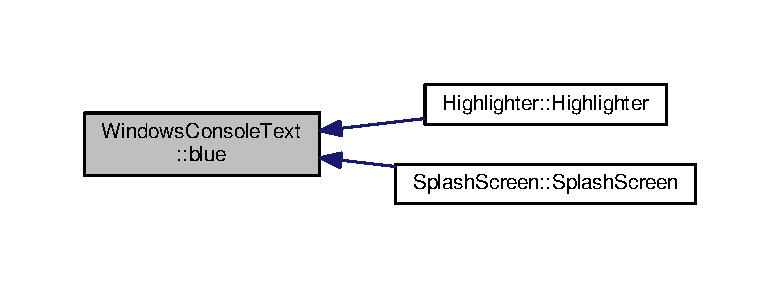
\includegraphics[width=350pt]{namespace_windows_console_text_a7bbbf356662bad883f5e777a14c89ed8_icgraph}
\end{center}
\end{figure}


\hypertarget{namespace_windows_console_text_a37e1e314abe02a10b3d55a66ba74c031}{\index{Windows\-Console\-Text@{Windows\-Console\-Text}!bold\-Blue@{bold\-Blue}}
\index{bold\-Blue@{bold\-Blue}!WindowsConsoleText@{Windows\-Console\-Text}}
\subsubsection[{bold\-Blue}]{\setlength{\rightskip}{0pt plus 5cm}string$\ast$ Windows\-Console\-Text\-::bold\-Blue (
\begin{DoxyParamCaption}
\item[{string $\ast$}]{text\-Str\-Ptr}
\end{DoxyParamCaption}
)}}\label{namespace_windows_console_text_a37e1e314abe02a10b3d55a66ba74c031}
Method to return bold blue text\-Str\-Ptr.


\begin{DoxyParams}{Parameters}
{\em text\-Str\-Ptr} & text\-Str\-Ptr to be printed bold blue. \\
\hline
\end{DoxyParams}
\begin{DoxyReturn}{Returns}
Bold blue text\-Str\-Ptr. 
\end{DoxyReturn}


Definition at line 67 of file Windows\-Console\-Text.\-cpp.

\hypertarget{namespace_windows_console_text_ad663bdad1383d48b6202cbe2d22f7c2e}{\index{Windows\-Console\-Text@{Windows\-Console\-Text}!bold\-Cyan@{bold\-Cyan}}
\index{bold\-Cyan@{bold\-Cyan}!WindowsConsoleText@{Windows\-Console\-Text}}
\subsubsection[{bold\-Cyan}]{\setlength{\rightskip}{0pt plus 5cm}string$\ast$ Windows\-Console\-Text\-::bold\-Cyan (
\begin{DoxyParamCaption}
\item[{string $\ast$}]{text\-Str\-Ptr}
\end{DoxyParamCaption}
)}}\label{namespace_windows_console_text_ad663bdad1383d48b6202cbe2d22f7c2e}
Method to return bold cyan text\-Str\-Ptr.


\begin{DoxyParams}{Parameters}
{\em text\-Str\-Ptr} & text\-Str\-Ptr to be printed bold cyan. \\
\hline
\end{DoxyParams}
\begin{DoxyReturn}{Returns}
Bold cyan text\-Str\-Ptr. 
\end{DoxyReturn}


Definition at line 79 of file Windows\-Console\-Text.\-cpp.

\hypertarget{namespace_windows_console_text_ae4eabe670d07ffade22db0e87aee5249}{\index{Windows\-Console\-Text@{Windows\-Console\-Text}!bold\-Gray@{bold\-Gray}}
\index{bold\-Gray@{bold\-Gray}!WindowsConsoleText@{Windows\-Console\-Text}}
\subsubsection[{bold\-Gray}]{\setlength{\rightskip}{0pt plus 5cm}string$\ast$ Windows\-Console\-Text\-::bold\-Gray (
\begin{DoxyParamCaption}
\item[{string $\ast$}]{text\-Str\-Ptr}
\end{DoxyParamCaption}
)}}\label{namespace_windows_console_text_ae4eabe670d07ffade22db0e87aee5249}
Method to return bold gray text\-Str\-Ptr.


\begin{DoxyParams}{Parameters}
{\em text\-Str\-Ptr} & text\-Str\-Ptr to be printed bold gray. \\
\hline
\end{DoxyParams}
\begin{DoxyReturn}{Returns}
Bold gray text\-Str\-Ptr. 
\end{DoxyReturn}


Definition at line 85 of file Windows\-Console\-Text.\-cpp.

\hypertarget{namespace_windows_console_text_aaec121e923f7ea5e3b7665c783044d1e}{\index{Windows\-Console\-Text@{Windows\-Console\-Text}!bold\-Green@{bold\-Green}}
\index{bold\-Green@{bold\-Green}!WindowsConsoleText@{Windows\-Console\-Text}}
\subsubsection[{bold\-Green}]{\setlength{\rightskip}{0pt plus 5cm}string$\ast$ Windows\-Console\-Text\-::bold\-Green (
\begin{DoxyParamCaption}
\item[{string $\ast$}]{text\-Str\-Ptr}
\end{DoxyParamCaption}
)}}\label{namespace_windows_console_text_aaec121e923f7ea5e3b7665c783044d1e}
Method to return bold green text\-Str\-Ptr.


\begin{DoxyParams}{Parameters}
{\em text\-Str\-Ptr} & text\-Str\-Ptr to be printed bold green. \\
\hline
\end{DoxyParams}
\begin{DoxyReturn}{Returns}
Bold green text\-Str\-Ptr. 
\end{DoxyReturn}


Definition at line 55 of file Windows\-Console\-Text.\-cpp.

\hypertarget{namespace_windows_console_text_a0157e7ea4c376fd86f05764d8c1242a1}{\index{Windows\-Console\-Text@{Windows\-Console\-Text}!bold\-Purple@{bold\-Purple}}
\index{bold\-Purple@{bold\-Purple}!WindowsConsoleText@{Windows\-Console\-Text}}
\subsubsection[{bold\-Purple}]{\setlength{\rightskip}{0pt plus 5cm}string$\ast$ Windows\-Console\-Text\-::bold\-Purple (
\begin{DoxyParamCaption}
\item[{string $\ast$}]{text\-Str\-Ptr}
\end{DoxyParamCaption}
)}}\label{namespace_windows_console_text_a0157e7ea4c376fd86f05764d8c1242a1}
Method to return bold purple text\-Str\-Ptr.


\begin{DoxyParams}{Parameters}
{\em text\-Str\-Ptr} & text\-Str\-Ptr to be printed bold purple. \\
\hline
\end{DoxyParams}
\begin{DoxyReturn}{Returns}
Bold purple text\-Str\-Ptr. 
\end{DoxyReturn}


Definition at line 73 of file Windows\-Console\-Text.\-cpp.

\hypertarget{namespace_windows_console_text_a4e7b50f0fec313c7e650eb0a70012c3e}{\index{Windows\-Console\-Text@{Windows\-Console\-Text}!bold\-Red@{bold\-Red}}
\index{bold\-Red@{bold\-Red}!WindowsConsoleText@{Windows\-Console\-Text}}
\subsubsection[{bold\-Red}]{\setlength{\rightskip}{0pt plus 5cm}string$\ast$ Windows\-Console\-Text\-::bold\-Red (
\begin{DoxyParamCaption}
\item[{string $\ast$}]{text\-Str\-Ptr}
\end{DoxyParamCaption}
)}}\label{namespace_windows_console_text_a4e7b50f0fec313c7e650eb0a70012c3e}
Method to return bold red text\-Str\-Ptr.


\begin{DoxyParams}{Parameters}
{\em text\-Str\-Ptr} & text\-Str\-Ptr to be printed bold red. \\
\hline
\end{DoxyParams}
\begin{DoxyReturn}{Returns}
Bold red text\-Str\-Ptr. 
\end{DoxyReturn}


Definition at line 49 of file Windows\-Console\-Text.\-cpp.

\hypertarget{namespace_windows_console_text_ab12845c763ce135aaa1e45efb61f49d9}{\index{Windows\-Console\-Text@{Windows\-Console\-Text}!bold\-Yellow@{bold\-Yellow}}
\index{bold\-Yellow@{bold\-Yellow}!WindowsConsoleText@{Windows\-Console\-Text}}
\subsubsection[{bold\-Yellow}]{\setlength{\rightskip}{0pt plus 5cm}string$\ast$ Windows\-Console\-Text\-::bold\-Yellow (
\begin{DoxyParamCaption}
\item[{string $\ast$}]{text\-Str\-Ptr}
\end{DoxyParamCaption}
)}}\label{namespace_windows_console_text_ab12845c763ce135aaa1e45efb61f49d9}
Method to return bold yellow text\-Str\-Ptr.


\begin{DoxyParams}{Parameters}
{\em text\-Str\-Ptr} & text\-Str\-Ptr to be printed bold yellow. \\
\hline
\end{DoxyParams}
\begin{DoxyReturn}{Returns}
Bold yellow text\-Str\-Ptr. 
\end{DoxyReturn}


Definition at line 61 of file Windows\-Console\-Text.\-cpp.

\hypertarget{namespace_windows_console_text_a4b1c94cd1e4282defb9baa7bf368fc64}{\index{Windows\-Console\-Text@{Windows\-Console\-Text}!cyan@{cyan}}
\index{cyan@{cyan}!WindowsConsoleText@{Windows\-Console\-Text}}
\subsubsection[{cyan}]{\setlength{\rightskip}{0pt plus 5cm}string$\ast$ Windows\-Console\-Text\-::cyan (
\begin{DoxyParamCaption}
\item[{string $\ast$}]{text\-Str\-Ptr}
\end{DoxyParamCaption}
)}}\label{namespace_windows_console_text_a4b1c94cd1e4282defb9baa7bf368fc64}
Method to return cyan text\-Str\-Ptr.


\begin{DoxyParams}{Parameters}
{\em text\-Str\-Ptr} & text\-Str\-Ptr to be printed cyan. \\
\hline
\end{DoxyParams}
\begin{DoxyReturn}{Returns}
Cyan text\-Str\-Ptr. 
\end{DoxyReturn}


Definition at line 34 of file Windows\-Console\-Text.\-cpp.

\hypertarget{namespace_windows_console_text_a71de428c5c1012768568a554909ce21e}{\index{Windows\-Console\-Text@{Windows\-Console\-Text}!gray@{gray}}
\index{gray@{gray}!WindowsConsoleText@{Windows\-Console\-Text}}
\subsubsection[{gray}]{\setlength{\rightskip}{0pt plus 5cm}string$\ast$ Windows\-Console\-Text\-::gray (
\begin{DoxyParamCaption}
\item[{string $\ast$}]{text\-Str\-Ptr}
\end{DoxyParamCaption}
)}}\label{namespace_windows_console_text_a71de428c5c1012768568a554909ce21e}
Method to return gray text\-Str\-Ptr.


\begin{DoxyParams}{Parameters}
{\em text\-Str\-Ptr} & text\-Str\-Ptr to be printed gray. \\
\hline
\end{DoxyParams}
\begin{DoxyReturn}{Returns}
Gray text\-Str\-Ptr. 
\end{DoxyReturn}


Definition at line 40 of file Windows\-Console\-Text.\-cpp.

\hypertarget{namespace_windows_console_text_a3b5e5879c4a73adde641f69b9c5c692b}{\index{Windows\-Console\-Text@{Windows\-Console\-Text}!green@{green}}
\index{green@{green}!WindowsConsoleText@{Windows\-Console\-Text}}
\subsubsection[{green}]{\setlength{\rightskip}{0pt plus 5cm}string$\ast$ Windows\-Console\-Text\-::green (
\begin{DoxyParamCaption}
\item[{string $\ast$}]{text\-Str\-Ptr}
\end{DoxyParamCaption}
)}}\label{namespace_windows_console_text_a3b5e5879c4a73adde641f69b9c5c692b}
Method to return green text\-Str\-Ptr.


\begin{DoxyParams}{Parameters}
{\em text\-Str\-Ptr} & text\-Str\-Ptr to be printed green. \\
\hline
\end{DoxyParams}
\begin{DoxyReturn}{Returns}
Green text\-Str\-Ptr. 
\end{DoxyReturn}


Definition at line 10 of file Windows\-Console\-Text.\-cpp.

\hypertarget{namespace_windows_console_text_a43e272994e8370c6cc1e8289872cc3f1}{\index{Windows\-Console\-Text@{Windows\-Console\-Text}!italic\-Blue@{italic\-Blue}}
\index{italic\-Blue@{italic\-Blue}!WindowsConsoleText@{Windows\-Console\-Text}}
\subsubsection[{italic\-Blue}]{\setlength{\rightskip}{0pt plus 5cm}string$\ast$ Windows\-Console\-Text\-::italic\-Blue (
\begin{DoxyParamCaption}
\item[{string $\ast$}]{text\-Str\-Ptr}
\end{DoxyParamCaption}
)}}\label{namespace_windows_console_text_a43e272994e8370c6cc1e8289872cc3f1}
Method to return italic blue text\-Str\-Ptr.


\begin{DoxyParams}{Parameters}
{\em text\-Str\-Ptr} & text\-Str\-Ptr to be printed italic blue. \\
\hline
\end{DoxyParams}
\begin{DoxyReturn}{Returns}
Italic blue text\-Str\-Ptr. 
\end{DoxyReturn}


Definition at line 112 of file Windows\-Console\-Text.\-cpp.

\hypertarget{namespace_windows_console_text_adeb5de271a3357ae4e3cca4faa7a2f1c}{\index{Windows\-Console\-Text@{Windows\-Console\-Text}!italic\-Cyan@{italic\-Cyan}}
\index{italic\-Cyan@{italic\-Cyan}!WindowsConsoleText@{Windows\-Console\-Text}}
\subsubsection[{italic\-Cyan}]{\setlength{\rightskip}{0pt plus 5cm}string$\ast$ Windows\-Console\-Text\-::italic\-Cyan (
\begin{DoxyParamCaption}
\item[{string $\ast$}]{text\-Str\-Ptr}
\end{DoxyParamCaption}
)}}\label{namespace_windows_console_text_adeb5de271a3357ae4e3cca4faa7a2f1c}
Method to return italic cyan text\-Str\-Ptr.


\begin{DoxyParams}{Parameters}
{\em text\-Str\-Ptr} & text\-Str\-Ptr to be printed italic cyan. \\
\hline
\end{DoxyParams}
\begin{DoxyReturn}{Returns}
Italic cyan text\-Str\-Ptr. 
\end{DoxyReturn}


Definition at line 124 of file Windows\-Console\-Text.\-cpp.

\hypertarget{namespace_windows_console_text_a4263561267b05b8eb062d4291ad48156}{\index{Windows\-Console\-Text@{Windows\-Console\-Text}!italic\-Gray@{italic\-Gray}}
\index{italic\-Gray@{italic\-Gray}!WindowsConsoleText@{Windows\-Console\-Text}}
\subsubsection[{italic\-Gray}]{\setlength{\rightskip}{0pt plus 5cm}string$\ast$ Windows\-Console\-Text\-::italic\-Gray (
\begin{DoxyParamCaption}
\item[{string $\ast$}]{text\-Str\-Ptr}
\end{DoxyParamCaption}
)}}\label{namespace_windows_console_text_a4263561267b05b8eb062d4291ad48156}
Method to return italic gray text\-Str\-Ptr.


\begin{DoxyParams}{Parameters}
{\em text\-Str\-Ptr} & text\-Str\-Ptr to be printed italic gray. \\
\hline
\end{DoxyParams}
\begin{DoxyReturn}{Returns}
Italic gray text\-Str\-Ptr. 
\end{DoxyReturn}


Definition at line 130 of file Windows\-Console\-Text.\-cpp.

\hypertarget{namespace_windows_console_text_ae8a44033301cf0b159f890bb17e9ade0}{\index{Windows\-Console\-Text@{Windows\-Console\-Text}!italic\-Green@{italic\-Green}}
\index{italic\-Green@{italic\-Green}!WindowsConsoleText@{Windows\-Console\-Text}}
\subsubsection[{italic\-Green}]{\setlength{\rightskip}{0pt plus 5cm}string$\ast$ Windows\-Console\-Text\-::italic\-Green (
\begin{DoxyParamCaption}
\item[{string $\ast$}]{text\-Str\-Ptr}
\end{DoxyParamCaption}
)}}\label{namespace_windows_console_text_ae8a44033301cf0b159f890bb17e9ade0}
Method to return italic green text\-Str\-Ptr.


\begin{DoxyParams}{Parameters}
{\em text\-Str\-Ptr} & text\-Str\-Ptr to be printed italic green. \\
\hline
\end{DoxyParams}
\begin{DoxyReturn}{Returns}
Italic green text\-Str\-Ptr. 
\end{DoxyReturn}


Definition at line 100 of file Windows\-Console\-Text.\-cpp.

\hypertarget{namespace_windows_console_text_a2ccdabfc1d8ffe166c063c039bd0a674}{\index{Windows\-Console\-Text@{Windows\-Console\-Text}!italic\-Purple@{italic\-Purple}}
\index{italic\-Purple@{italic\-Purple}!WindowsConsoleText@{Windows\-Console\-Text}}
\subsubsection[{italic\-Purple}]{\setlength{\rightskip}{0pt plus 5cm}string$\ast$ Windows\-Console\-Text\-::italic\-Purple (
\begin{DoxyParamCaption}
\item[{string $\ast$}]{text\-Str\-Ptr}
\end{DoxyParamCaption}
)}}\label{namespace_windows_console_text_a2ccdabfc1d8ffe166c063c039bd0a674}
Method to return italic purple text\-Str\-Ptr.


\begin{DoxyParams}{Parameters}
{\em text\-Str\-Ptr} & text\-Str\-Ptr to be printed italic purple. \\
\hline
\end{DoxyParams}
\begin{DoxyReturn}{Returns}
Italic purple text\-Str\-Ptr. 
\end{DoxyReturn}


Definition at line 118 of file Windows\-Console\-Text.\-cpp.

\hypertarget{namespace_windows_console_text_a71db4269f200b021de61913d2b7903f2}{\index{Windows\-Console\-Text@{Windows\-Console\-Text}!italic\-Red@{italic\-Red}}
\index{italic\-Red@{italic\-Red}!WindowsConsoleText@{Windows\-Console\-Text}}
\subsubsection[{italic\-Red}]{\setlength{\rightskip}{0pt plus 5cm}string$\ast$ Windows\-Console\-Text\-::italic\-Red (
\begin{DoxyParamCaption}
\item[{string $\ast$}]{text\-Str\-Ptr}
\end{DoxyParamCaption}
)}}\label{namespace_windows_console_text_a71db4269f200b021de61913d2b7903f2}
Method to return italic red text\-Str\-Ptr.


\begin{DoxyParams}{Parameters}
{\em text\-Str\-Ptr} & text\-Str\-Ptr to be printed italic red. \\
\hline
\end{DoxyParams}
\begin{DoxyReturn}{Returns}
Italic red text\-Str\-Ptr. 
\end{DoxyReturn}


Definition at line 94 of file Windows\-Console\-Text.\-cpp.

\hypertarget{namespace_windows_console_text_af7505c56ac71c073a30f9c7497ea5dd8}{\index{Windows\-Console\-Text@{Windows\-Console\-Text}!italic\-Yellow@{italic\-Yellow}}
\index{italic\-Yellow@{italic\-Yellow}!WindowsConsoleText@{Windows\-Console\-Text}}
\subsubsection[{italic\-Yellow}]{\setlength{\rightskip}{0pt plus 5cm}string$\ast$ Windows\-Console\-Text\-::italic\-Yellow (
\begin{DoxyParamCaption}
\item[{string $\ast$}]{text\-Str\-Ptr}
\end{DoxyParamCaption}
)}}\label{namespace_windows_console_text_af7505c56ac71c073a30f9c7497ea5dd8}
Method to return italic yellow text\-Str\-Ptr.


\begin{DoxyParams}{Parameters}
{\em text\-Str\-Ptr} & text\-Str\-Ptr to be printed italic yellow. \\
\hline
\end{DoxyParams}
\begin{DoxyReturn}{Returns}
Italic yellow text\-Str\-Ptr. 
\end{DoxyReturn}


Definition at line 106 of file Windows\-Console\-Text.\-cpp.

\hypertarget{namespace_windows_console_text_aff0abcf384e233f425332c77a07a45ac}{\index{Windows\-Console\-Text@{Windows\-Console\-Text}!purple@{purple}}
\index{purple@{purple}!WindowsConsoleText@{Windows\-Console\-Text}}
\subsubsection[{purple}]{\setlength{\rightskip}{0pt plus 5cm}string$\ast$ Windows\-Console\-Text\-::purple (
\begin{DoxyParamCaption}
\item[{string $\ast$}]{text\-Str\-Ptr}
\end{DoxyParamCaption}
)}}\label{namespace_windows_console_text_aff0abcf384e233f425332c77a07a45ac}
Method to return purple text\-Str\-Ptr.


\begin{DoxyParams}{Parameters}
{\em text\-Str\-Ptr} & text\-Str\-Ptr to be printed purple. \\
\hline
\end{DoxyParams}
\begin{DoxyReturn}{Returns}
Purple text\-Str\-Ptr. 
\end{DoxyReturn}


Definition at line 28 of file Windows\-Console\-Text.\-cpp.

\hypertarget{namespace_windows_console_text_a0b3bd4d8c412a8208762be06cf2c7ddd}{\index{Windows\-Console\-Text@{Windows\-Console\-Text}!red@{red}}
\index{red@{red}!WindowsConsoleText@{Windows\-Console\-Text}}
\subsubsection[{red}]{\setlength{\rightskip}{0pt plus 5cm}string$\ast$ Windows\-Console\-Text\-::red (
\begin{DoxyParamCaption}
\item[{string $\ast$}]{text\-Str\-Ptr}
\end{DoxyParamCaption}
)}}\label{namespace_windows_console_text_a0b3bd4d8c412a8208762be06cf2c7ddd}
Method to return red text\-Str\-Ptr.


\begin{DoxyParams}{Parameters}
{\em text\-Str\-Ptr} & text\-Str\-Ptr to be printed red. \\
\hline
\end{DoxyParams}
\begin{DoxyReturn}{Returns}
Red text\-Str\-Ptr. 
\end{DoxyReturn}


Definition at line 4 of file Windows\-Console\-Text.\-cpp.



Here is the caller graph for this function\-:
\nopagebreak
\begin{figure}[H]
\begin{center}
\leavevmode
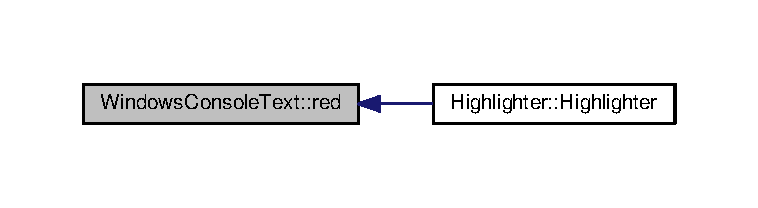
\includegraphics[width=350pt]{namespace_windows_console_text_a0b3bd4d8c412a8208762be06cf2c7ddd_icgraph}
\end{center}
\end{figure}


\hypertarget{namespace_windows_console_text_a318921dc20bbc206b4c20f5c20fcd01f}{\index{Windows\-Console\-Text@{Windows\-Console\-Text}!underlined\-Blue@{underlined\-Blue}}
\index{underlined\-Blue@{underlined\-Blue}!WindowsConsoleText@{Windows\-Console\-Text}}
\subsubsection[{underlined\-Blue}]{\setlength{\rightskip}{0pt plus 5cm}string$\ast$ Windows\-Console\-Text\-::underlined\-Blue (
\begin{DoxyParamCaption}
\item[{string $\ast$}]{text\-Str\-Ptr}
\end{DoxyParamCaption}
)}}\label{namespace_windows_console_text_a318921dc20bbc206b4c20f5c20fcd01f}
Method to return underlined blue text\-Str\-Ptr.


\begin{DoxyParams}{Parameters}
{\em text\-Str\-Ptr} & text\-Str\-Ptr to be printed underlined blue. \\
\hline
\end{DoxyParams}
\begin{DoxyReturn}{Returns}
Underlined blue text\-Str\-Ptr. 
\end{DoxyReturn}


Definition at line 157 of file Windows\-Console\-Text.\-cpp.

\hypertarget{namespace_windows_console_text_a20c98475a28eb10d06e9dd2a6259ce5b}{\index{Windows\-Console\-Text@{Windows\-Console\-Text}!underlined\-Cyan@{underlined\-Cyan}}
\index{underlined\-Cyan@{underlined\-Cyan}!WindowsConsoleText@{Windows\-Console\-Text}}
\subsubsection[{underlined\-Cyan}]{\setlength{\rightskip}{0pt plus 5cm}string$\ast$ Windows\-Console\-Text\-::underlined\-Cyan (
\begin{DoxyParamCaption}
\item[{string $\ast$}]{text\-Str\-Ptr}
\end{DoxyParamCaption}
)}}\label{namespace_windows_console_text_a20c98475a28eb10d06e9dd2a6259ce5b}
Method to return underlined cyan text\-Str\-Ptr.


\begin{DoxyParams}{Parameters}
{\em text\-Str\-Ptr} & text\-Str\-Ptr to be printed underlined cyan. \\
\hline
\end{DoxyParams}
\begin{DoxyReturn}{Returns}
Underlined cyan text\-Str\-Ptr. 
\end{DoxyReturn}


Definition at line 169 of file Windows\-Console\-Text.\-cpp.

\hypertarget{namespace_windows_console_text_acc55d1a6037d60c533ebfb742b594b9f}{\index{Windows\-Console\-Text@{Windows\-Console\-Text}!underlined\-Gray@{underlined\-Gray}}
\index{underlined\-Gray@{underlined\-Gray}!WindowsConsoleText@{Windows\-Console\-Text}}
\subsubsection[{underlined\-Gray}]{\setlength{\rightskip}{0pt plus 5cm}string$\ast$ Windows\-Console\-Text\-::underlined\-Gray (
\begin{DoxyParamCaption}
\item[{string $\ast$}]{text\-Str\-Ptr}
\end{DoxyParamCaption}
)}}\label{namespace_windows_console_text_acc55d1a6037d60c533ebfb742b594b9f}
Method to return underlined gray text\-Str\-Ptr.


\begin{DoxyParams}{Parameters}
{\em text\-Str\-Ptr} & text\-Str\-Ptr to be printed underlined gray. \\
\hline
\end{DoxyParams}
\begin{DoxyReturn}{Returns}
Underlined gray text\-Str\-Ptr. 
\end{DoxyReturn}


Definition at line 175 of file Windows\-Console\-Text.\-cpp.

\hypertarget{namespace_windows_console_text_ae2d3c6f156dfd20fbcaf002f60c3063a}{\index{Windows\-Console\-Text@{Windows\-Console\-Text}!underlined\-Green@{underlined\-Green}}
\index{underlined\-Green@{underlined\-Green}!WindowsConsoleText@{Windows\-Console\-Text}}
\subsubsection[{underlined\-Green}]{\setlength{\rightskip}{0pt plus 5cm}string$\ast$ Windows\-Console\-Text\-::underlined\-Green (
\begin{DoxyParamCaption}
\item[{string $\ast$}]{text\-Str\-Ptr}
\end{DoxyParamCaption}
)}}\label{namespace_windows_console_text_ae2d3c6f156dfd20fbcaf002f60c3063a}
Method to return underlined green text\-Str\-Ptr.


\begin{DoxyParams}{Parameters}
{\em text\-Str\-Ptr} & text\-Str\-Ptr to be printed underlined green. \\
\hline
\end{DoxyParams}
\begin{DoxyReturn}{Returns}
Underlined green text\-Str\-Ptr. 
\end{DoxyReturn}


Definition at line 145 of file Windows\-Console\-Text.\-cpp.

\hypertarget{namespace_windows_console_text_adddcdb4ed3b84b741d98d0e1ea2e4921}{\index{Windows\-Console\-Text@{Windows\-Console\-Text}!underlined\-Purple@{underlined\-Purple}}
\index{underlined\-Purple@{underlined\-Purple}!WindowsConsoleText@{Windows\-Console\-Text}}
\subsubsection[{underlined\-Purple}]{\setlength{\rightskip}{0pt plus 5cm}string$\ast$ Windows\-Console\-Text\-::underlined\-Purple (
\begin{DoxyParamCaption}
\item[{string $\ast$}]{text\-Str\-Ptr}
\end{DoxyParamCaption}
)}}\label{namespace_windows_console_text_adddcdb4ed3b84b741d98d0e1ea2e4921}
Method to return underlined purple text\-Str\-Ptr.


\begin{DoxyParams}{Parameters}
{\em text\-Str\-Ptr} & text\-Str\-Ptr to be printed underlined purple. \\
\hline
\end{DoxyParams}
\begin{DoxyReturn}{Returns}
Underlined purple text\-Str\-Ptr. 
\end{DoxyReturn}


Definition at line 163 of file Windows\-Console\-Text.\-cpp.

\hypertarget{namespace_windows_console_text_a58b2e71e3c82e6a5fd9470d94fd0e339}{\index{Windows\-Console\-Text@{Windows\-Console\-Text}!underlined\-Red@{underlined\-Red}}
\index{underlined\-Red@{underlined\-Red}!WindowsConsoleText@{Windows\-Console\-Text}}
\subsubsection[{underlined\-Red}]{\setlength{\rightskip}{0pt plus 5cm}string$\ast$ Windows\-Console\-Text\-::underlined\-Red (
\begin{DoxyParamCaption}
\item[{string $\ast$}]{text\-Str\-Ptr}
\end{DoxyParamCaption}
)}}\label{namespace_windows_console_text_a58b2e71e3c82e6a5fd9470d94fd0e339}
Method to return underlined red text\-Str\-Ptr.


\begin{DoxyParams}{Parameters}
{\em text\-Str\-Ptr} & text\-Str\-Ptr to be printed underlined red. \\
\hline
\end{DoxyParams}
\begin{DoxyReturn}{Returns}
Underlined red text\-Str\-Ptr. 
\end{DoxyReturn}


Definition at line 139 of file Windows\-Console\-Text.\-cpp.

\hypertarget{namespace_windows_console_text_ae57c84df042a9ea941f83edd16e3c24a}{\index{Windows\-Console\-Text@{Windows\-Console\-Text}!underlined\-Yellow@{underlined\-Yellow}}
\index{underlined\-Yellow@{underlined\-Yellow}!WindowsConsoleText@{Windows\-Console\-Text}}
\subsubsection[{underlined\-Yellow}]{\setlength{\rightskip}{0pt plus 5cm}string$\ast$ Windows\-Console\-Text\-::underlined\-Yellow (
\begin{DoxyParamCaption}
\item[{string $\ast$}]{text\-Str\-Ptr}
\end{DoxyParamCaption}
)}}\label{namespace_windows_console_text_ae57c84df042a9ea941f83edd16e3c24a}
Method to return underlined yellow text\-Str\-Ptr.


\begin{DoxyParams}{Parameters}
{\em text\-Str\-Ptr} & text\-Str\-Ptr to be printed underlined yellow. \\
\hline
\end{DoxyParams}
\begin{DoxyReturn}{Returns}
Underlined yellow text\-Str\-Ptr. 
\end{DoxyReturn}


Definition at line 151 of file Windows\-Console\-Text.\-cpp.

\hypertarget{namespace_windows_console_text_a13969e6a4cdad5b49196fb843585fef2}{\index{Windows\-Console\-Text@{Windows\-Console\-Text}!yellow@{yellow}}
\index{yellow@{yellow}!WindowsConsoleText@{Windows\-Console\-Text}}
\subsubsection[{yellow}]{\setlength{\rightskip}{0pt plus 5cm}string$\ast$ Windows\-Console\-Text\-::yellow (
\begin{DoxyParamCaption}
\item[{string $\ast$}]{text\-Str\-Ptr}
\end{DoxyParamCaption}
)}}\label{namespace_windows_console_text_a13969e6a4cdad5b49196fb843585fef2}
Method to return yellow text\-Str\-Ptr.


\begin{DoxyParams}{Parameters}
{\em text\-Str\-Ptr} & text\-Str\-Ptr to be printed yellow. \\
\hline
\end{DoxyParams}
\begin{DoxyReturn}{Returns}
Yellow text\-Str\-Ptr. 
\end{DoxyReturn}


Definition at line 16 of file Windows\-Console\-Text.\-cpp.


\hypertarget{namespace_xml_master}{\section{Xml\-Master Namespace Reference}
\label{namespace_xml_master}\index{Xml\-Master@{Xml\-Master}}
}
\subsection*{Functions}
\begin{DoxyCompactItemize}
\item 
void \hyperlink{namespace_xml_master_ad6410c6eca04a1184a0f1fd90c75f0c9}{insert\-After\-Last\-Occurrence} (Q\-File $\ast$file\-Ptr, Q\-String $\ast$occurrence\-Of\-Str\-Ptr, Q\-String $\ast$insertion\-Str\-Ptr)
\end{DoxyCompactItemize}


\subsection{Function Documentation}
\hypertarget{namespace_xml_master_ad6410c6eca04a1184a0f1fd90c75f0c9}{\index{Xml\-Master@{Xml\-Master}!insert\-After\-Last\-Occurrence@{insert\-After\-Last\-Occurrence}}
\index{insert\-After\-Last\-Occurrence@{insert\-After\-Last\-Occurrence}!XmlMaster@{Xml\-Master}}
\subsubsection[{insert\-After\-Last\-Occurrence}]{\setlength{\rightskip}{0pt plus 5cm}void Xml\-Master\-::insert\-After\-Last\-Occurrence (
\begin{DoxyParamCaption}
\item[{Q\-File $\ast$}]{file\-Ptr, }
\item[{Q\-String $\ast$}]{occurrence\-Of\-Str\-Ptr, }
\item[{Q\-String $\ast$}]{insertion\-Str\-Ptr}
\end{DoxyParamCaption}
)}}\label{namespace_xml_master_ad6410c6eca04a1184a0f1fd90c75f0c9}


Definition at line 4 of file Xml\-Master.\-cpp.


\chapter{Class Documentation}
\hypertarget{class_build}{\section{Build Class Reference}
\label{class_build}\index{Build@{Build}}
}


{\ttfamily \#include $<$Build.\-h$>$}

\subsection*{Public Member Functions}
\begin{DoxyCompactItemize}
\item 
\hyperlink{class_build_a96ad56fb129cfbc2131fd094c41ae1ec}{Build} ()
\item 
void \hyperlink{class_build_a00566c3a17a753ca8722b63c5905528a}{run\-Build\-Cmd} ()
\item 
\hyperlink{class_build_a8f1d400e9bc158b6339cc1785b18d07b}{$\sim$\-Build} ()
\end{DoxyCompactItemize}
\subsection*{Private Attributes}
\begin{DoxyCompactItemize}
\item 
const Q\-String $\ast$ \hyperlink{class_build_a32d97560bba88abe53398fdebcb4ddcf}{P\-K\-G\-\_\-\-O\-P\-T\-I\-O\-N\-\_\-\-S\-T\-R\-\_\-\-P\-T\-R}
\item 
Q\-String\-List $\ast$ \hyperlink{class_build_af980a5b63ef5778e733cc4d29064be7e}{pkg\-Str\-Lst\-Ptr}
\item 
Q\-Process $\ast$ \hyperlink{class_build_aa71d3581eeb4b8c05a99cd01d16e7994}{build\-Process\-Ptr}
\end{DoxyCompactItemize}


\subsection{Detailed Description}


Definition at line 27 of file Build.\-h.



\subsection{Constructor \& Destructor Documentation}
\hypertarget{class_build_a96ad56fb129cfbc2131fd094c41ae1ec}{\index{Build@{Build}!Build@{Build}}
\index{Build@{Build}!Build@{Build}}
\subsubsection[{Build}]{\setlength{\rightskip}{0pt plus 5cm}Build\-::\-Build (
\begin{DoxyParamCaption}
{}
\end{DoxyParamCaption}
)}}\label{class_build_a96ad56fb129cfbc2131fd094c41ae1ec}


Definition at line 4 of file Build.\-cpp.

\hypertarget{class_build_a8f1d400e9bc158b6339cc1785b18d07b}{\index{Build@{Build}!$\sim$\-Build@{$\sim$\-Build}}
\index{$\sim$\-Build@{$\sim$\-Build}!Build@{Build}}
\subsubsection[{$\sim$\-Build}]{\setlength{\rightskip}{0pt plus 5cm}Build\-::$\sim$\-Build (
\begin{DoxyParamCaption}
{}
\end{DoxyParamCaption}
)}}\label{class_build_a8f1d400e9bc158b6339cc1785b18d07b}


Definition at line 19 of file Build.\-cpp.



\subsection{Member Function Documentation}
\hypertarget{class_build_a00566c3a17a753ca8722b63c5905528a}{\index{Build@{Build}!run\-Build\-Cmd@{run\-Build\-Cmd}}
\index{run\-Build\-Cmd@{run\-Build\-Cmd}!Build@{Build}}
\subsubsection[{run\-Build\-Cmd}]{\setlength{\rightskip}{0pt plus 5cm}void Build\-::run\-Build\-Cmd (
\begin{DoxyParamCaption}
{}
\end{DoxyParamCaption}
)}}\label{class_build_a00566c3a17a753ca8722b63c5905528a}


Definition at line 12 of file Build.\-cpp.



\subsection{Member Data Documentation}
\hypertarget{class_build_aa71d3581eeb4b8c05a99cd01d16e7994}{\index{Build@{Build}!build\-Process\-Ptr@{build\-Process\-Ptr}}
\index{build\-Process\-Ptr@{build\-Process\-Ptr}!Build@{Build}}
\subsubsection[{build\-Process\-Ptr}]{\setlength{\rightskip}{0pt plus 5cm}Q\-Process$\ast$ Build\-::build\-Process\-Ptr\hspace{0.3cm}{\ttfamily [private]}}}\label{class_build_aa71d3581eeb4b8c05a99cd01d16e7994}


Definition at line 32 of file Build.\-h.

\hypertarget{class_build_a32d97560bba88abe53398fdebcb4ddcf}{\index{Build@{Build}!P\-K\-G\-\_\-\-O\-P\-T\-I\-O\-N\-\_\-\-S\-T\-R\-\_\-\-P\-T\-R@{P\-K\-G\-\_\-\-O\-P\-T\-I\-O\-N\-\_\-\-S\-T\-R\-\_\-\-P\-T\-R}}
\index{P\-K\-G\-\_\-\-O\-P\-T\-I\-O\-N\-\_\-\-S\-T\-R\-\_\-\-P\-T\-R@{P\-K\-G\-\_\-\-O\-P\-T\-I\-O\-N\-\_\-\-S\-T\-R\-\_\-\-P\-T\-R}!Build@{Build}}
\subsubsection[{P\-K\-G\-\_\-\-O\-P\-T\-I\-O\-N\-\_\-\-S\-T\-R\-\_\-\-P\-T\-R}]{\setlength{\rightskip}{0pt plus 5cm}const Q\-String$\ast$ Build\-::\-P\-K\-G\-\_\-\-O\-P\-T\-I\-O\-N\-\_\-\-S\-T\-R\-\_\-\-P\-T\-R\hspace{0.3cm}{\ttfamily [private]}}}\label{class_build_a32d97560bba88abe53398fdebcb4ddcf}


Definition at line 30 of file Build.\-h.

\hypertarget{class_build_af980a5b63ef5778e733cc4d29064be7e}{\index{Build@{Build}!pkg\-Str\-Lst\-Ptr@{pkg\-Str\-Lst\-Ptr}}
\index{pkg\-Str\-Lst\-Ptr@{pkg\-Str\-Lst\-Ptr}!Build@{Build}}
\subsubsection[{pkg\-Str\-Lst\-Ptr}]{\setlength{\rightskip}{0pt plus 5cm}Q\-String\-List$\ast$ Build\-::pkg\-Str\-Lst\-Ptr\hspace{0.3cm}{\ttfamily [private]}}}\label{class_build_af980a5b63ef5778e733cc4d29064be7e}


Definition at line 31 of file Build.\-h.



The documentation for this class was generated from the following files\-:\begin{DoxyCompactItemize}
\item 
/home/james/\-Net\-Beans\-Projects/ride/src/\hyperlink{_build_8h}{Build.\-h}\item 
/home/james/\-Net\-Beans\-Projects/ride/src/\hyperlink{_build_8cpp}{Build.\-cpp}\end{DoxyCompactItemize}

\hypertarget{class_central_gui}{\section{Central\-Gui Class Reference}
\label{class_central_gui}\index{Central\-Gui@{Central\-Gui}}
}


{\ttfamily \#include $<$Central\-Gui.\-h$>$}



Inheritance diagram for Central\-Gui\-:\nopagebreak
\begin{figure}[H]
\begin{center}
\leavevmode
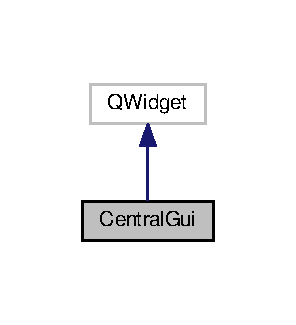
\includegraphics[width=142pt]{class_central_gui__inherit__graph}
\end{center}
\end{figure}


Collaboration diagram for Central\-Gui\-:\nopagebreak
\begin{figure}[H]
\begin{center}
\leavevmode
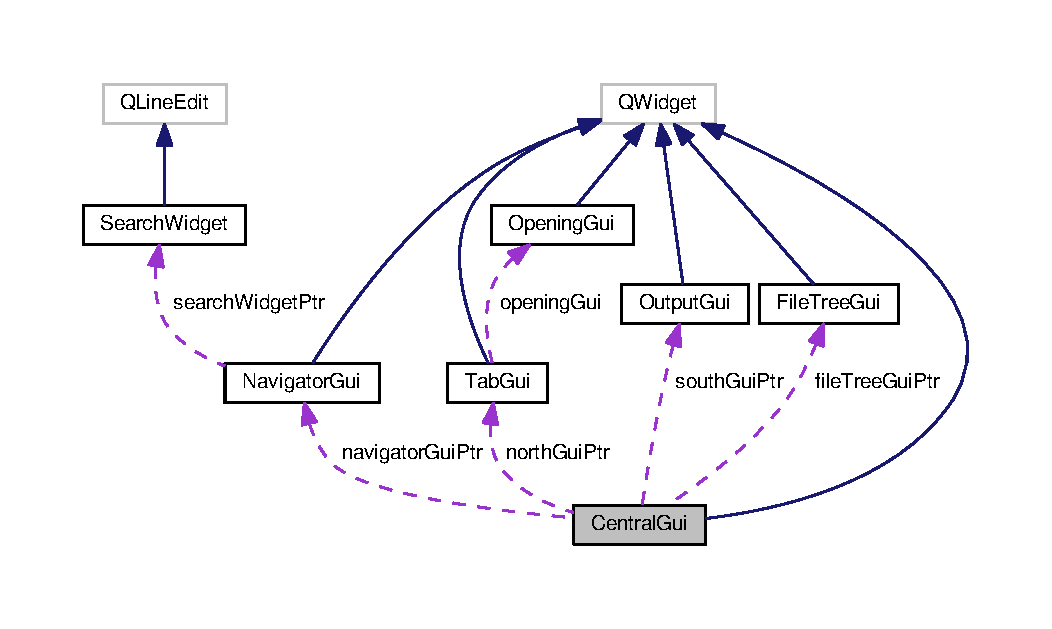
\includegraphics[width=346pt]{class_central_gui__coll__graph}
\end{center}
\end{figure}
\subsection*{Public Member Functions}
\begin{DoxyCompactItemize}
\item 
\hyperlink{class_central_gui_aba31873e4b5d4bf9fd1e563601efc4e7}{Central\-Gui} (Q\-Widget $\ast$parent=0)
\item 
void \hyperlink{class_central_gui_afb70afe6db1411c77956236188e67bd0}{set\-Central\-Tabs\-Ptr} (\hyperlink{class_tab_gui}{Tab\-Gui} $\ast$\hyperlink{class_central_gui_a8ec49e2c3a7c601bed4a7e4ccf173682}{central\-Tabs\-Ptr})
\item 
\hyperlink{class_tab_gui}{Tab\-Gui} $\ast$ \hyperlink{class_central_gui_a16716c4c66f7ce8e4552fcb20337ab39}{get\-Central\-Tabs\-Ptr} ()
\item 
void \hyperlink{class_central_gui_a65abd3c9dc8bb14a60ca89da399c427e}{set\-File\-Tree\-Gui\-Ptr} (\hyperlink{class_file_tree_gui}{File\-Tree\-Gui} $\ast$\hyperlink{class_central_gui_a6abfae93daa17e3af2a814888c9c14cf}{file\-Tree\-Gui\-Ptr})
\item 
\hyperlink{class_file_tree_gui}{File\-Tree\-Gui} $\ast$ \hyperlink{class_central_gui_aba7129fa7a935565409beb63498c2eb3}{get\-File\-Tree\-Gui\-Ptr} ()
\item 
void \hyperlink{class_central_gui_ae8559c5a3733e33a1ded21db79bd8d3a}{set\-Output\-Gui\-Ptr} (\hyperlink{class_output_gui}{Output\-Gui} $\ast$\hyperlink{class_central_gui_a60c563767906a6db0c209f0b21437a09}{output\-Gui\-Ptr})
\item 
\hyperlink{class_output_gui}{Output\-Gui} $\ast$ \hyperlink{class_central_gui_a47d2d46581f064ed8b46e1f611a0bd98}{get\-Output\-Gui\-Ptr} ()
\item 
void \hyperlink{class_central_gui_a8f7149e1e5b7cfc5c694421482c68c5e}{pass\-Master\-Tab\-Widget\-Ptr} (Q\-Tab\-Widget $\ast$master\-Tab\-Widget\-Ptr)
\item 
\hyperlink{class_central_gui_ad54c2077e29d7a2017399b39e62c1043}{$\sim$\-Central\-Gui} ()
\end{DoxyCompactItemize}
\subsection*{Private Attributes}
\begin{DoxyCompactItemize}
\item 
\hyperlink{class_tab_gui}{Tab\-Gui} $\ast$ \hyperlink{class_central_gui_a8ec49e2c3a7c601bed4a7e4ccf173682}{central\-Tabs\-Ptr}
\item 
\hyperlink{class_file_tree_gui}{File\-Tree\-Gui} $\ast$ \hyperlink{class_central_gui_a6abfae93daa17e3af2a814888c9c14cf}{file\-Tree\-Gui\-Ptr}
\item 
\hyperlink{class_output_gui}{Output\-Gui} $\ast$ \hyperlink{class_central_gui_a60c563767906a6db0c209f0b21437a09}{output\-Gui\-Ptr}
\item 
Q\-Grid\-Layout $\ast$ \hyperlink{class_central_gui_ab10e8028968ca8d5bf7b2cfe4b257d52}{outer\-Layout}
\end{DoxyCompactItemize}


\subsection{Detailed Description}


Definition at line 26 of file Central\-Gui.\-h.



\subsection{Constructor \& Destructor Documentation}
\hypertarget{class_central_gui_aba31873e4b5d4bf9fd1e563601efc4e7}{\index{Central\-Gui@{Central\-Gui}!Central\-Gui@{Central\-Gui}}
\index{Central\-Gui@{Central\-Gui}!CentralGui@{Central\-Gui}}
\subsubsection[{Central\-Gui}]{\setlength{\rightskip}{0pt plus 5cm}Central\-Gui\-::\-Central\-Gui (
\begin{DoxyParamCaption}
\item[{Q\-Widget $\ast$}]{parent = {\ttfamily 0}}
\end{DoxyParamCaption}
)}}\label{class_central_gui_aba31873e4b5d4bf9fd1e563601efc4e7}


Definition at line 4 of file Central\-Gui.\-cpp.

\hypertarget{class_central_gui_ad54c2077e29d7a2017399b39e62c1043}{\index{Central\-Gui@{Central\-Gui}!$\sim$\-Central\-Gui@{$\sim$\-Central\-Gui}}
\index{$\sim$\-Central\-Gui@{$\sim$\-Central\-Gui}!CentralGui@{Central\-Gui}}
\subsubsection[{$\sim$\-Central\-Gui}]{\setlength{\rightskip}{0pt plus 5cm}Central\-Gui\-::$\sim$\-Central\-Gui (
\begin{DoxyParamCaption}
{}
\end{DoxyParamCaption}
)}}\label{class_central_gui_ad54c2077e29d7a2017399b39e62c1043}


Definition at line 69 of file Central\-Gui.\-cpp.



\subsection{Member Function Documentation}
\hypertarget{class_central_gui_a16716c4c66f7ce8e4552fcb20337ab39}{\index{Central\-Gui@{Central\-Gui}!get\-Central\-Tabs\-Ptr@{get\-Central\-Tabs\-Ptr}}
\index{get\-Central\-Tabs\-Ptr@{get\-Central\-Tabs\-Ptr}!CentralGui@{Central\-Gui}}
\subsubsection[{get\-Central\-Tabs\-Ptr}]{\setlength{\rightskip}{0pt plus 5cm}{\bf Tab\-Gui} $\ast$ Central\-Gui\-::get\-Central\-Tabs\-Ptr (
\begin{DoxyParamCaption}
{}
\end{DoxyParamCaption}
)}}\label{class_central_gui_a16716c4c66f7ce8e4552fcb20337ab39}


Definition at line 33 of file Central\-Gui.\-cpp.

\hypertarget{class_central_gui_aba7129fa7a935565409beb63498c2eb3}{\index{Central\-Gui@{Central\-Gui}!get\-File\-Tree\-Gui\-Ptr@{get\-File\-Tree\-Gui\-Ptr}}
\index{get\-File\-Tree\-Gui\-Ptr@{get\-File\-Tree\-Gui\-Ptr}!CentralGui@{Central\-Gui}}
\subsubsection[{get\-File\-Tree\-Gui\-Ptr}]{\setlength{\rightskip}{0pt plus 5cm}{\bf File\-Tree\-Gui} $\ast$ Central\-Gui\-::get\-File\-Tree\-Gui\-Ptr (
\begin{DoxyParamCaption}
{}
\end{DoxyParamCaption}
)}}\label{class_central_gui_aba7129fa7a935565409beb63498c2eb3}


Definition at line 45 of file Central\-Gui.\-cpp.

\hypertarget{class_central_gui_a47d2d46581f064ed8b46e1f611a0bd98}{\index{Central\-Gui@{Central\-Gui}!get\-Output\-Gui\-Ptr@{get\-Output\-Gui\-Ptr}}
\index{get\-Output\-Gui\-Ptr@{get\-Output\-Gui\-Ptr}!CentralGui@{Central\-Gui}}
\subsubsection[{get\-Output\-Gui\-Ptr}]{\setlength{\rightskip}{0pt plus 5cm}{\bf Output\-Gui} $\ast$ Central\-Gui\-::get\-Output\-Gui\-Ptr (
\begin{DoxyParamCaption}
{}
\end{DoxyParamCaption}
)}}\label{class_central_gui_a47d2d46581f064ed8b46e1f611a0bd98}


Definition at line 57 of file Central\-Gui.\-cpp.

\hypertarget{class_central_gui_a8f7149e1e5b7cfc5c694421482c68c5e}{\index{Central\-Gui@{Central\-Gui}!pass\-Master\-Tab\-Widget\-Ptr@{pass\-Master\-Tab\-Widget\-Ptr}}
\index{pass\-Master\-Tab\-Widget\-Ptr@{pass\-Master\-Tab\-Widget\-Ptr}!CentralGui@{Central\-Gui}}
\subsubsection[{pass\-Master\-Tab\-Widget\-Ptr}]{\setlength{\rightskip}{0pt plus 5cm}void Central\-Gui\-::pass\-Master\-Tab\-Widget\-Ptr (
\begin{DoxyParamCaption}
\item[{Q\-Tab\-Widget $\ast$}]{master\-Tab\-Widget\-Ptr}
\end{DoxyParamCaption}
)}}\label{class_central_gui_a8f7149e1e5b7cfc5c694421482c68c5e}


Definition at line 63 of file Central\-Gui.\-cpp.

\hypertarget{class_central_gui_afb70afe6db1411c77956236188e67bd0}{\index{Central\-Gui@{Central\-Gui}!set\-Central\-Tabs\-Ptr@{set\-Central\-Tabs\-Ptr}}
\index{set\-Central\-Tabs\-Ptr@{set\-Central\-Tabs\-Ptr}!CentralGui@{Central\-Gui}}
\subsubsection[{set\-Central\-Tabs\-Ptr}]{\setlength{\rightskip}{0pt plus 5cm}void Central\-Gui\-::set\-Central\-Tabs\-Ptr (
\begin{DoxyParamCaption}
\item[{{\bf Tab\-Gui} $\ast$}]{central\-Tabs\-Ptr}
\end{DoxyParamCaption}
)}}\label{class_central_gui_afb70afe6db1411c77956236188e67bd0}


Definition at line 27 of file Central\-Gui.\-cpp.

\hypertarget{class_central_gui_a65abd3c9dc8bb14a60ca89da399c427e}{\index{Central\-Gui@{Central\-Gui}!set\-File\-Tree\-Gui\-Ptr@{set\-File\-Tree\-Gui\-Ptr}}
\index{set\-File\-Tree\-Gui\-Ptr@{set\-File\-Tree\-Gui\-Ptr}!CentralGui@{Central\-Gui}}
\subsubsection[{set\-File\-Tree\-Gui\-Ptr}]{\setlength{\rightskip}{0pt plus 5cm}void Central\-Gui\-::set\-File\-Tree\-Gui\-Ptr (
\begin{DoxyParamCaption}
\item[{{\bf File\-Tree\-Gui} $\ast$}]{file\-Tree\-Gui\-Ptr}
\end{DoxyParamCaption}
)}}\label{class_central_gui_a65abd3c9dc8bb14a60ca89da399c427e}


Definition at line 39 of file Central\-Gui.\-cpp.

\hypertarget{class_central_gui_ae8559c5a3733e33a1ded21db79bd8d3a}{\index{Central\-Gui@{Central\-Gui}!set\-Output\-Gui\-Ptr@{set\-Output\-Gui\-Ptr}}
\index{set\-Output\-Gui\-Ptr@{set\-Output\-Gui\-Ptr}!CentralGui@{Central\-Gui}}
\subsubsection[{set\-Output\-Gui\-Ptr}]{\setlength{\rightskip}{0pt plus 5cm}void Central\-Gui\-::set\-Output\-Gui\-Ptr (
\begin{DoxyParamCaption}
\item[{{\bf Output\-Gui} $\ast$}]{output\-Gui\-Ptr}
\end{DoxyParamCaption}
)}}\label{class_central_gui_ae8559c5a3733e33a1ded21db79bd8d3a}


Definition at line 51 of file Central\-Gui.\-cpp.



\subsection{Member Data Documentation}
\hypertarget{class_central_gui_a8ec49e2c3a7c601bed4a7e4ccf173682}{\index{Central\-Gui@{Central\-Gui}!central\-Tabs\-Ptr@{central\-Tabs\-Ptr}}
\index{central\-Tabs\-Ptr@{central\-Tabs\-Ptr}!CentralGui@{Central\-Gui}}
\subsubsection[{central\-Tabs\-Ptr}]{\setlength{\rightskip}{0pt plus 5cm}{\bf Tab\-Gui}$\ast$ Central\-Gui\-::central\-Tabs\-Ptr\hspace{0.3cm}{\ttfamily [private]}}}\label{class_central_gui_a8ec49e2c3a7c601bed4a7e4ccf173682}


Definition at line 31 of file Central\-Gui.\-h.

\hypertarget{class_central_gui_a6abfae93daa17e3af2a814888c9c14cf}{\index{Central\-Gui@{Central\-Gui}!file\-Tree\-Gui\-Ptr@{file\-Tree\-Gui\-Ptr}}
\index{file\-Tree\-Gui\-Ptr@{file\-Tree\-Gui\-Ptr}!CentralGui@{Central\-Gui}}
\subsubsection[{file\-Tree\-Gui\-Ptr}]{\setlength{\rightskip}{0pt plus 5cm}{\bf File\-Tree\-Gui}$\ast$ Central\-Gui\-::file\-Tree\-Gui\-Ptr\hspace{0.3cm}{\ttfamily [private]}}}\label{class_central_gui_a6abfae93daa17e3af2a814888c9c14cf}


Definition at line 32 of file Central\-Gui.\-h.

\hypertarget{class_central_gui_ab10e8028968ca8d5bf7b2cfe4b257d52}{\index{Central\-Gui@{Central\-Gui}!outer\-Layout@{outer\-Layout}}
\index{outer\-Layout@{outer\-Layout}!CentralGui@{Central\-Gui}}
\subsubsection[{outer\-Layout}]{\setlength{\rightskip}{0pt plus 5cm}Q\-Grid\-Layout$\ast$ Central\-Gui\-::outer\-Layout\hspace{0.3cm}{\ttfamily [private]}}}\label{class_central_gui_ab10e8028968ca8d5bf7b2cfe4b257d52}


Definition at line 35 of file Central\-Gui.\-h.

\hypertarget{class_central_gui_a60c563767906a6db0c209f0b21437a09}{\index{Central\-Gui@{Central\-Gui}!output\-Gui\-Ptr@{output\-Gui\-Ptr}}
\index{output\-Gui\-Ptr@{output\-Gui\-Ptr}!CentralGui@{Central\-Gui}}
\subsubsection[{output\-Gui\-Ptr}]{\setlength{\rightskip}{0pt plus 5cm}{\bf Output\-Gui}$\ast$ Central\-Gui\-::output\-Gui\-Ptr\hspace{0.3cm}{\ttfamily [private]}}}\label{class_central_gui_a60c563767906a6db0c209f0b21437a09}


Definition at line 33 of file Central\-Gui.\-h.



The documentation for this class was generated from the following files\-:\begin{DoxyCompactItemize}
\item 
/home/james/\-Net\-Beans\-Projects/ride/src/\hyperlink{_central_gui_8h}{Central\-Gui.\-h}\item 
/home/james/\-Net\-Beans\-Projects/ride/src/\hyperlink{_central_gui_8cpp}{Central\-Gui.\-cpp}\end{DoxyCompactItemize}

\hypertarget{class_directory}{\section{Directory Class Reference}
\label{class_directory}\index{Directory@{Directory}}
}


{\ttfamily \#include $<$Directory.\-h$>$}



Inheritance diagram for Directory\-:\nopagebreak
\begin{figure}[H]
\begin{center}
\leavevmode
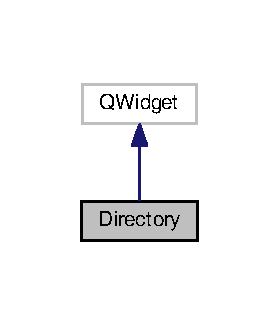
\includegraphics[width=134pt]{class_directory__inherit__graph}
\end{center}
\end{figure}


Collaboration diagram for Directory\-:\nopagebreak
\begin{figure}[H]
\begin{center}
\leavevmode
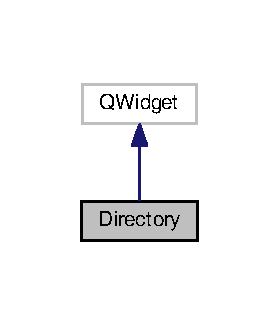
\includegraphics[width=134pt]{class_directory__coll__graph}
\end{center}
\end{figure}
\subsection*{Public Member Functions}
\begin{DoxyCompactItemize}
\item 
\hyperlink{class_directory_aeecdbc52ed5d2069d57c8e5618a73f1e}{Directory} (Q\-Widget $\ast$parent=0)
\item 
void \hyperlink{class_directory_ad17ee176714d11afae82e7bf20def5a5}{set\-Dir\-Ptr} (Q\-Dir $\ast$\hyperlink{class_directory_ae8d40a5989c8fe90988aa9517cb87a9a}{dir\-Ptr})
\item 
Q\-Dir $\ast$ \hyperlink{class_directory_a1ae52186cc94eee26fc6161b67dd0ba2}{get\-Dir\-Ptr} ()
\item 
void \hyperlink{class_directory_af3cac89c90ab3097e7a7a36be6b12c64}{set\-Dir\-Type\-Ptr} (\hyperlink{class_directory_a1c40bdd8c03ef51a29fa097c325fe345}{Dir\-Type} $\ast$\hyperlink{class_directory_aeb912c1ed24b2bea1febce142fa3a57e}{dir\-Type\-Ptr})
\item 
\hyperlink{class_directory_a1c40bdd8c03ef51a29fa097c325fe345}{Dir\-Type} $\ast$ \hyperlink{class_directory_ae44daf13fc34b0b1e1d4198feec67a94}{get\-Dir\-Type\-Ptr} ()
\item 
void \hyperlink{class_directory_a4ba19180f0e71eb407d93e6b83ea7802}{push\-Back\-To\-Child\-Dirs\-Ptr\-Vec} (Q\-Dir $\ast$dir)
\item 
Q\-Vector$<$ Q\-Dir $\ast$ $>$ \hyperlink{class_directory_ab6f2b6cdc1da5fb168743cdfbece2f87}{get\-Child\-Dirs\-Ptr\-Vec} ()
\item 
void \hyperlink{class_directory_a9d5365aa51a62931af93272d97ea2b85}{push\-Back\-To\-Child\-Files\-Ptr\-Vec} (Q\-File $\ast$file)
\item 
Q\-Vector$<$ Q\-File $\ast$ $>$ \hyperlink{class_directory_a769dcd01a9476d1556384c1572156a04}{get\-Child\-Files\-Ptr\-Vec} ()
\item 
Q\-String $\ast$ \hyperlink{class_directory_a4f0ef25beff4469b7eb06765a0b1fa26}{to\-String} ()
\item 
\hyperlink{class_directory_affbde8714685c61601421097d621341d}{$\sim$\-Directory} ()
\end{DoxyCompactItemize}
\subsection*{Private Types}
\begin{DoxyCompactItemize}
\item 
enum \hyperlink{class_directory_a1c40bdd8c03ef51a29fa097c325fe345}{Dir\-Type} \{ \\*
\hyperlink{class_directory_a1c40bdd8c03ef51a29fa097c325fe345a032f30deac97c5bda25698f881b31b16}{N\-O\-D\-E}, 
\hyperlink{class_directory_a1c40bdd8c03ef51a29fa097c325fe345a04113739df8828cf617628d4409d246b}{S\-R\-C}, 
\hyperlink{class_directory_a1c40bdd8c03ef51a29fa097c325fe345a398cbd150a21421197b733b2a71620b4}{I\-N\-C\-L\-U\-D\-E}, 
\hyperlink{class_directory_a1c40bdd8c03ef51a29fa097c325fe345a5eadd6da197b9497d88d759f877d1a6e}{B\-U\-I\-L\-D}, 
\\*
\hyperlink{class_directory_a1c40bdd8c03ef51a29fa097c325fe345ae99347ac7c31d8d87215e88a3805d136}{D\-E\-V\-E\-L}, 
\hyperlink{class_directory_a1c40bdd8c03ef51a29fa097c325fe345af0bbf2abf7d54499e138b6a3448f05f8}{O\-T\-H\-E\-R}
 \}
\end{DoxyCompactItemize}
\subsection*{Private Attributes}
\begin{DoxyCompactItemize}
\item 
Q\-Dir $\ast$ \hyperlink{class_directory_ae8d40a5989c8fe90988aa9517cb87a9a}{dir\-Ptr}
\item 
\hyperlink{class_directory_a1c40bdd8c03ef51a29fa097c325fe345}{Dir\-Type} $\ast$ \hyperlink{class_directory_aeb912c1ed24b2bea1febce142fa3a57e}{dir\-Type\-Ptr}
\item 
Q\-Vector$<$ Q\-Dir $\ast$ $>$ \hyperlink{class_directory_a46f528b377bd9738da7c5a4ff9bb643e}{child\-Dirs\-Ptr\-Vec}
\item 
Q\-Vector$<$ Q\-File $\ast$ $>$ \hyperlink{class_directory_a3dcbd1171a1c28867b8c718bb0ecf5ff}{child\-Files\-Ptr\-Vec}
\end{DoxyCompactItemize}


\subsection{Detailed Description}


Definition at line 25 of file Directory.\-h.



\subsection{Member Enumeration Documentation}
\hypertarget{class_directory_a1c40bdd8c03ef51a29fa097c325fe345}{\index{Directory@{Directory}!Dir\-Type@{Dir\-Type}}
\index{Dir\-Type@{Dir\-Type}!Directory@{Directory}}
\subsubsection[{Dir\-Type}]{\setlength{\rightskip}{0pt plus 5cm}enum {\bf Directory\-::\-Dir\-Type}\hspace{0.3cm}{\ttfamily [private]}}}\label{class_directory_a1c40bdd8c03ef51a29fa097c325fe345}
\begin{Desc}
\item[Enumerator]\par
\begin{description}
\index{N\-O\-D\-E@{N\-O\-D\-E}!Directory@{Directory}}\index{Directory@{Directory}!N\-O\-D\-E@{N\-O\-D\-E}}\item[{\em 
\hypertarget{class_directory_a1c40bdd8c03ef51a29fa097c325fe345a032f30deac97c5bda25698f881b31b16}{N\-O\-D\-E}\label{class_directory_a1c40bdd8c03ef51a29fa097c325fe345a032f30deac97c5bda25698f881b31b16}
}]\index{S\-R\-C@{S\-R\-C}!Directory@{Directory}}\index{Directory@{Directory}!S\-R\-C@{S\-R\-C}}\item[{\em 
\hypertarget{class_directory_a1c40bdd8c03ef51a29fa097c325fe345a04113739df8828cf617628d4409d246b}{S\-R\-C}\label{class_directory_a1c40bdd8c03ef51a29fa097c325fe345a04113739df8828cf617628d4409d246b}
}]\index{I\-N\-C\-L\-U\-D\-E@{I\-N\-C\-L\-U\-D\-E}!Directory@{Directory}}\index{Directory@{Directory}!I\-N\-C\-L\-U\-D\-E@{I\-N\-C\-L\-U\-D\-E}}\item[{\em 
\hypertarget{class_directory_a1c40bdd8c03ef51a29fa097c325fe345a398cbd150a21421197b733b2a71620b4}{I\-N\-C\-L\-U\-D\-E}\label{class_directory_a1c40bdd8c03ef51a29fa097c325fe345a398cbd150a21421197b733b2a71620b4}
}]\index{B\-U\-I\-L\-D@{B\-U\-I\-L\-D}!Directory@{Directory}}\index{Directory@{Directory}!B\-U\-I\-L\-D@{B\-U\-I\-L\-D}}\item[{\em 
\hypertarget{class_directory_a1c40bdd8c03ef51a29fa097c325fe345a5eadd6da197b9497d88d759f877d1a6e}{B\-U\-I\-L\-D}\label{class_directory_a1c40bdd8c03ef51a29fa097c325fe345a5eadd6da197b9497d88d759f877d1a6e}
}]\index{D\-E\-V\-E\-L@{D\-E\-V\-E\-L}!Directory@{Directory}}\index{Directory@{Directory}!D\-E\-V\-E\-L@{D\-E\-V\-E\-L}}\item[{\em 
\hypertarget{class_directory_a1c40bdd8c03ef51a29fa097c325fe345ae99347ac7c31d8d87215e88a3805d136}{D\-E\-V\-E\-L}\label{class_directory_a1c40bdd8c03ef51a29fa097c325fe345ae99347ac7c31d8d87215e88a3805d136}
}]\index{O\-T\-H\-E\-R@{O\-T\-H\-E\-R}!Directory@{Directory}}\index{Directory@{Directory}!O\-T\-H\-E\-R@{O\-T\-H\-E\-R}}\item[{\em 
\hypertarget{class_directory_a1c40bdd8c03ef51a29fa097c325fe345af0bbf2abf7d54499e138b6a3448f05f8}{O\-T\-H\-E\-R}\label{class_directory_a1c40bdd8c03ef51a29fa097c325fe345af0bbf2abf7d54499e138b6a3448f05f8}
}]\end{description}
\end{Desc}


Definition at line 30 of file Directory.\-h.



\subsection{Constructor \& Destructor Documentation}
\hypertarget{class_directory_aeecdbc52ed5d2069d57c8e5618a73f1e}{\index{Directory@{Directory}!Directory@{Directory}}
\index{Directory@{Directory}!Directory@{Directory}}
\subsubsection[{Directory}]{\setlength{\rightskip}{0pt plus 5cm}Directory\-::\-Directory (
\begin{DoxyParamCaption}
\item[{Q\-Widget $\ast$}]{parent = {\ttfamily 0}}
\end{DoxyParamCaption}
)}}\label{class_directory_aeecdbc52ed5d2069d57c8e5618a73f1e}


Definition at line 4 of file Directory.\-cpp.

\hypertarget{class_directory_affbde8714685c61601421097d621341d}{\index{Directory@{Directory}!$\sim$\-Directory@{$\sim$\-Directory}}
\index{$\sim$\-Directory@{$\sim$\-Directory}!Directory@{Directory}}
\subsubsection[{$\sim$\-Directory}]{\setlength{\rightskip}{0pt plus 5cm}Directory\-::$\sim$\-Directory (
\begin{DoxyParamCaption}
{}
\end{DoxyParamCaption}
)}}\label{class_directory_affbde8714685c61601421097d621341d}


Definition at line 86 of file Directory.\-cpp.



\subsection{Member Function Documentation}
\hypertarget{class_directory_ab6f2b6cdc1da5fb168743cdfbece2f87}{\index{Directory@{Directory}!get\-Child\-Dirs\-Ptr\-Vec@{get\-Child\-Dirs\-Ptr\-Vec}}
\index{get\-Child\-Dirs\-Ptr\-Vec@{get\-Child\-Dirs\-Ptr\-Vec}!Directory@{Directory}}
\subsubsection[{get\-Child\-Dirs\-Ptr\-Vec}]{\setlength{\rightskip}{0pt plus 5cm}Q\-Vector$<$ Q\-Dir $\ast$ $>$ Directory\-::get\-Child\-Dirs\-Ptr\-Vec (
\begin{DoxyParamCaption}
{}
\end{DoxyParamCaption}
)}}\label{class_directory_ab6f2b6cdc1da5fb168743cdfbece2f87}


Definition at line 40 of file Directory.\-cpp.

\hypertarget{class_directory_a769dcd01a9476d1556384c1572156a04}{\index{Directory@{Directory}!get\-Child\-Files\-Ptr\-Vec@{get\-Child\-Files\-Ptr\-Vec}}
\index{get\-Child\-Files\-Ptr\-Vec@{get\-Child\-Files\-Ptr\-Vec}!Directory@{Directory}}
\subsubsection[{get\-Child\-Files\-Ptr\-Vec}]{\setlength{\rightskip}{0pt plus 5cm}Q\-Vector$<$ Q\-File $\ast$ $>$ Directory\-::get\-Child\-Files\-Ptr\-Vec (
\begin{DoxyParamCaption}
{}
\end{DoxyParamCaption}
)}}\label{class_directory_a769dcd01a9476d1556384c1572156a04}


Definition at line 52 of file Directory.\-cpp.

\hypertarget{class_directory_a1ae52186cc94eee26fc6161b67dd0ba2}{\index{Directory@{Directory}!get\-Dir\-Ptr@{get\-Dir\-Ptr}}
\index{get\-Dir\-Ptr@{get\-Dir\-Ptr}!Directory@{Directory}}
\subsubsection[{get\-Dir\-Ptr}]{\setlength{\rightskip}{0pt plus 5cm}Q\-Dir $\ast$ Directory\-::get\-Dir\-Ptr (
\begin{DoxyParamCaption}
{}
\end{DoxyParamCaption}
)}}\label{class_directory_a1ae52186cc94eee26fc6161b67dd0ba2}


Definition at line 16 of file Directory.\-cpp.

\hypertarget{class_directory_ae44daf13fc34b0b1e1d4198feec67a94}{\index{Directory@{Directory}!get\-Dir\-Type\-Ptr@{get\-Dir\-Type\-Ptr}}
\index{get\-Dir\-Type\-Ptr@{get\-Dir\-Type\-Ptr}!Directory@{Directory}}
\subsubsection[{get\-Dir\-Type\-Ptr}]{\setlength{\rightskip}{0pt plus 5cm}{\bf Directory\-::\-Dir\-Type} $\ast$ Directory\-::get\-Dir\-Type\-Ptr (
\begin{DoxyParamCaption}
{}
\end{DoxyParamCaption}
)}}\label{class_directory_ae44daf13fc34b0b1e1d4198feec67a94}


Definition at line 28 of file Directory.\-cpp.

\hypertarget{class_directory_a4ba19180f0e71eb407d93e6b83ea7802}{\index{Directory@{Directory}!push\-Back\-To\-Child\-Dirs\-Ptr\-Vec@{push\-Back\-To\-Child\-Dirs\-Ptr\-Vec}}
\index{push\-Back\-To\-Child\-Dirs\-Ptr\-Vec@{push\-Back\-To\-Child\-Dirs\-Ptr\-Vec}!Directory@{Directory}}
\subsubsection[{push\-Back\-To\-Child\-Dirs\-Ptr\-Vec}]{\setlength{\rightskip}{0pt plus 5cm}void Directory\-::push\-Back\-To\-Child\-Dirs\-Ptr\-Vec (
\begin{DoxyParamCaption}
\item[{Q\-Dir $\ast$}]{dir}
\end{DoxyParamCaption}
)}}\label{class_directory_a4ba19180f0e71eb407d93e6b83ea7802}


Definition at line 34 of file Directory.\-cpp.

\hypertarget{class_directory_a9d5365aa51a62931af93272d97ea2b85}{\index{Directory@{Directory}!push\-Back\-To\-Child\-Files\-Ptr\-Vec@{push\-Back\-To\-Child\-Files\-Ptr\-Vec}}
\index{push\-Back\-To\-Child\-Files\-Ptr\-Vec@{push\-Back\-To\-Child\-Files\-Ptr\-Vec}!Directory@{Directory}}
\subsubsection[{push\-Back\-To\-Child\-Files\-Ptr\-Vec}]{\setlength{\rightskip}{0pt plus 5cm}void Directory\-::push\-Back\-To\-Child\-Files\-Ptr\-Vec (
\begin{DoxyParamCaption}
\item[{Q\-File $\ast$}]{file}
\end{DoxyParamCaption}
)}}\label{class_directory_a9d5365aa51a62931af93272d97ea2b85}


Definition at line 46 of file Directory.\-cpp.

\hypertarget{class_directory_ad17ee176714d11afae82e7bf20def5a5}{\index{Directory@{Directory}!set\-Dir\-Ptr@{set\-Dir\-Ptr}}
\index{set\-Dir\-Ptr@{set\-Dir\-Ptr}!Directory@{Directory}}
\subsubsection[{set\-Dir\-Ptr}]{\setlength{\rightskip}{0pt plus 5cm}void Directory\-::set\-Dir\-Ptr (
\begin{DoxyParamCaption}
\item[{Q\-Dir $\ast$}]{dir\-Ptr}
\end{DoxyParamCaption}
)}}\label{class_directory_ad17ee176714d11afae82e7bf20def5a5}


Definition at line 10 of file Directory.\-cpp.

\hypertarget{class_directory_af3cac89c90ab3097e7a7a36be6b12c64}{\index{Directory@{Directory}!set\-Dir\-Type\-Ptr@{set\-Dir\-Type\-Ptr}}
\index{set\-Dir\-Type\-Ptr@{set\-Dir\-Type\-Ptr}!Directory@{Directory}}
\subsubsection[{set\-Dir\-Type\-Ptr}]{\setlength{\rightskip}{0pt plus 5cm}void Directory\-::set\-Dir\-Type\-Ptr (
\begin{DoxyParamCaption}
\item[{{\bf Directory\-::\-Dir\-Type} $\ast$}]{dir\-Type\-Ptr}
\end{DoxyParamCaption}
)}}\label{class_directory_af3cac89c90ab3097e7a7a36be6b12c64}


Definition at line 22 of file Directory.\-cpp.

\hypertarget{class_directory_a4f0ef25beff4469b7eb06765a0b1fa26}{\index{Directory@{Directory}!to\-String@{to\-String}}
\index{to\-String@{to\-String}!Directory@{Directory}}
\subsubsection[{to\-String}]{\setlength{\rightskip}{0pt plus 5cm}Q\-String $\ast$ Directory\-::to\-String (
\begin{DoxyParamCaption}
{}
\end{DoxyParamCaption}
)}}\label{class_directory_a4f0ef25beff4469b7eb06765a0b1fa26}


Definition at line 58 of file Directory.\-cpp.



\subsection{Member Data Documentation}
\hypertarget{class_directory_a46f528b377bd9738da7c5a4ff9bb643e}{\index{Directory@{Directory}!child\-Dirs\-Ptr\-Vec@{child\-Dirs\-Ptr\-Vec}}
\index{child\-Dirs\-Ptr\-Vec@{child\-Dirs\-Ptr\-Vec}!Directory@{Directory}}
\subsubsection[{child\-Dirs\-Ptr\-Vec}]{\setlength{\rightskip}{0pt plus 5cm}Q\-Vector$<$Q\-Dir$\ast$$>$ Directory\-::child\-Dirs\-Ptr\-Vec\hspace{0.3cm}{\ttfamily [private]}}}\label{class_directory_a46f528b377bd9738da7c5a4ff9bb643e}


Definition at line 42 of file Directory.\-h.

\hypertarget{class_directory_a3dcbd1171a1c28867b8c718bb0ecf5ff}{\index{Directory@{Directory}!child\-Files\-Ptr\-Vec@{child\-Files\-Ptr\-Vec}}
\index{child\-Files\-Ptr\-Vec@{child\-Files\-Ptr\-Vec}!Directory@{Directory}}
\subsubsection[{child\-Files\-Ptr\-Vec}]{\setlength{\rightskip}{0pt plus 5cm}Q\-Vector$<$Q\-File$\ast$$>$ Directory\-::child\-Files\-Ptr\-Vec\hspace{0.3cm}{\ttfamily [private]}}}\label{class_directory_a3dcbd1171a1c28867b8c718bb0ecf5ff}


Definition at line 43 of file Directory.\-h.

\hypertarget{class_directory_ae8d40a5989c8fe90988aa9517cb87a9a}{\index{Directory@{Directory}!dir\-Ptr@{dir\-Ptr}}
\index{dir\-Ptr@{dir\-Ptr}!Directory@{Directory}}
\subsubsection[{dir\-Ptr}]{\setlength{\rightskip}{0pt plus 5cm}Q\-Dir$\ast$ Directory\-::dir\-Ptr\hspace{0.3cm}{\ttfamily [private]}}}\label{class_directory_ae8d40a5989c8fe90988aa9517cb87a9a}


Definition at line 40 of file Directory.\-h.

\hypertarget{class_directory_aeb912c1ed24b2bea1febce142fa3a57e}{\index{Directory@{Directory}!dir\-Type\-Ptr@{dir\-Type\-Ptr}}
\index{dir\-Type\-Ptr@{dir\-Type\-Ptr}!Directory@{Directory}}
\subsubsection[{dir\-Type\-Ptr}]{\setlength{\rightskip}{0pt plus 5cm}{\bf Dir\-Type}$\ast$ Directory\-::dir\-Type\-Ptr\hspace{0.3cm}{\ttfamily [private]}}}\label{class_directory_aeb912c1ed24b2bea1febce142fa3a57e}


Definition at line 41 of file Directory.\-h.



The documentation for this class was generated from the following files\-:\begin{DoxyCompactItemize}
\item 
/home/james/\-Net\-Beans\-Projects/ride/src/\hyperlink{_directory_8h}{Directory.\-h}\item 
/home/james/\-Net\-Beans\-Projects/ride/src/\hyperlink{_directory_8cpp}{Directory.\-cpp}\end{DoxyCompactItemize}

\hypertarget{class_file_gui}{\section{File\-Gui Class Reference}
\label{class_file_gui}\index{File\-Gui@{File\-Gui}}
}


{\ttfamily \#include $<$File\-Gui.\-h$>$}

Inheritance diagram for File\-Gui\-:\begin{figure}[H]
\begin{center}
\leavevmode
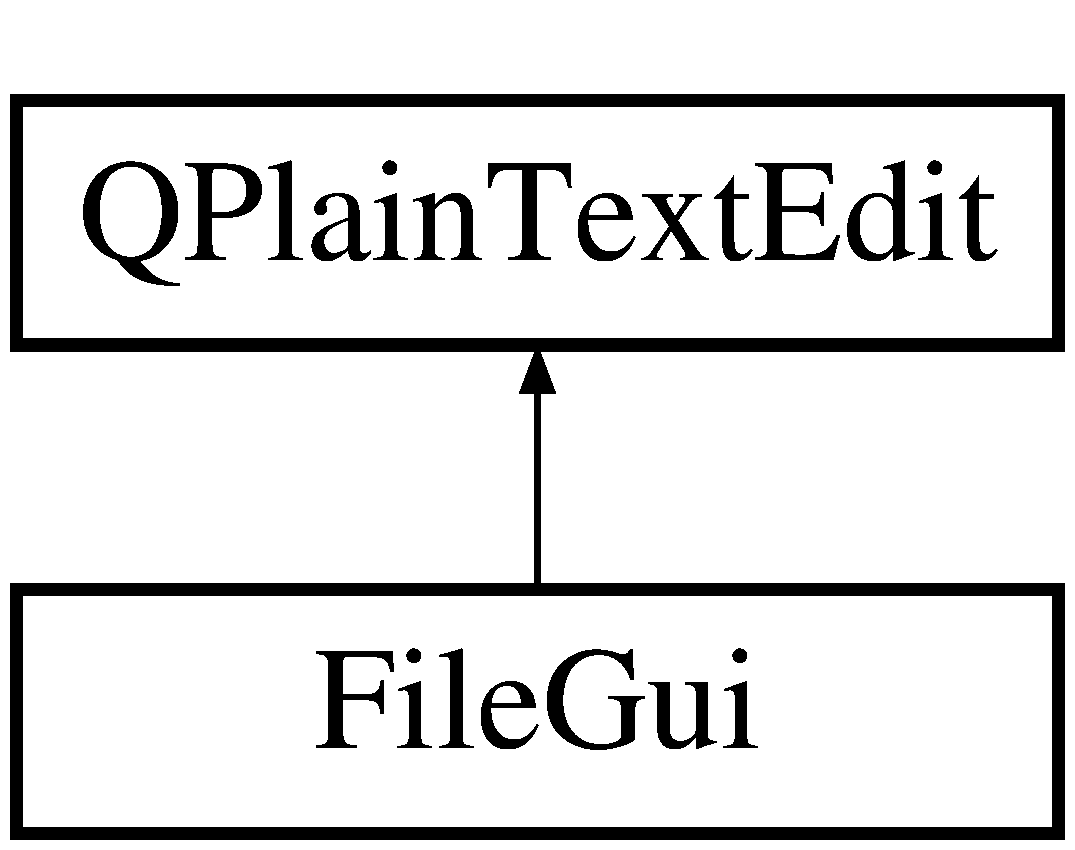
\includegraphics[height=2.000000cm]{class_file_gui}
\end{center}
\end{figure}
\subsection*{Public Member Functions}
\begin{DoxyCompactItemize}
\item 
\hyperlink{class_file_gui_ac7c9b0cdbb2e89190a13318ec84c70a3}{File\-Gui} (Q\-Widget $\ast$parent=0)
\item 
void \hyperlink{class_file_gui_ab95b0b24bfee919e33bcf6c623c72842}{set\-Completer} (Q\-Completer $\ast$\hyperlink{class_file_gui_a71dfac2e67bf84af494667901b51ddc9}{c})
\item 
Q\-Completer $\ast$ \hyperlink{class_file_gui_a741c813e12ed8105bc9b30aa0a48c4d7}{completer} () const 
\item 
void \hyperlink{class_file_gui_a24940e7e57f49e81c451f137acfbe60a}{line\-Number\-Area\-Paint\-Event} (Q\-Paint\-Event $\ast$event)
\item 
int \hyperlink{class_file_gui_af5ea5edc018ed2ba6685ae6e5244483f}{line\-Number\-Area\-Width} ()
\item 
void \hyperlink{class_file_gui_a704d37c450e30eeb506a89f7e5b7a79e}{resize\-Event} (Q\-Resize\-Event $\ast$event)
\item 
Q\-String $\ast$ \hyperlink{class_file_gui_a0d31bd4f4169eff45e59fa79ba4e98f9}{to\-String} ()
\item 
\hyperlink{class_file_gui_a276b681a3fbd10e083463e32a361461c}{$\sim$\-File\-Gui} ()
\end{DoxyCompactItemize}
\subsection*{Protected Member Functions}
\begin{DoxyCompactItemize}
\item 
void \hyperlink{class_file_gui_aed2ed675e3d0eec814fda21479babb36}{key\-Press\-Event} (Q\-Key\-Event $\ast$e)
\end{DoxyCompactItemize}
\subsection*{Private Slots}
\begin{DoxyCompactItemize}
\item 
void \hyperlink{class_file_gui_a5b90c98b648fc77ef8474152e6632af3}{insert\-Completion} (const Q\-String \&completion)
\item 
void \hyperlink{class_file_gui_a498aa60814cc9265695e656e9b7a2e87}{update\-Line\-Number\-Area\-Width} (int new\-Block\-Count)
\item 
void \hyperlink{class_file_gui_a04e7291acb7167a70377f53dd7bd47f4}{highlight\-Current\-Line} ()
\item 
void \hyperlink{class_file_gui_ae1ce22662fb60a146101e8768acca3f1}{update\-Line\-Number\-Area} (const Q\-Rect \&, int)
\end{DoxyCompactItemize}
\subsection*{Private Member Functions}
\begin{DoxyCompactItemize}
\item 
Q\-String \hyperlink{class_file_gui_a3d263213e8a442878876eef041325493}{word\-Under\-Cursor} () const 
\end{DoxyCompactItemize}
\subsection*{Private Attributes}
\begin{DoxyCompactItemize}
\item 
Q\-Widget $\ast$ \hyperlink{class_file_gui_a4fa030b7bda34eeb961eac7324f28b88}{line\-Number\-Area}
\item 
Q\-Completer $\ast$ \hyperlink{class_file_gui_a71dfac2e67bf84af494667901b51ddc9}{c}
\end{DoxyCompactItemize}


\subsection{Constructor \& Destructor Documentation}
\hypertarget{class_file_gui_ac7c9b0cdbb2e89190a13318ec84c70a3}{\index{File\-Gui@{File\-Gui}!File\-Gui@{File\-Gui}}
\index{File\-Gui@{File\-Gui}!FileGui@{File\-Gui}}
\subsubsection[{File\-Gui}]{\setlength{\rightskip}{0pt plus 5cm}File\-Gui\-::\-File\-Gui (
\begin{DoxyParamCaption}
\item[{Q\-Widget $\ast$}]{parent = {\ttfamily 0}}
\end{DoxyParamCaption}
)}}\label{class_file_gui_ac7c9b0cdbb2e89190a13318ec84c70a3}
\hypertarget{class_file_gui_a276b681a3fbd10e083463e32a361461c}{\index{File\-Gui@{File\-Gui}!$\sim$\-File\-Gui@{$\sim$\-File\-Gui}}
\index{$\sim$\-File\-Gui@{$\sim$\-File\-Gui}!FileGui@{File\-Gui}}
\subsubsection[{$\sim$\-File\-Gui}]{\setlength{\rightskip}{0pt plus 5cm}File\-Gui\-::$\sim$\-File\-Gui (
\begin{DoxyParamCaption}
{}
\end{DoxyParamCaption}
)}}\label{class_file_gui_a276b681a3fbd10e083463e32a361461c}


\subsection{Member Function Documentation}
\hypertarget{class_file_gui_a741c813e12ed8105bc9b30aa0a48c4d7}{\index{File\-Gui@{File\-Gui}!completer@{completer}}
\index{completer@{completer}!FileGui@{File\-Gui}}
\subsubsection[{completer}]{\setlength{\rightskip}{0pt plus 5cm}Q\-Completer $\ast$ File\-Gui\-::completer (
\begin{DoxyParamCaption}
{}
\end{DoxyParamCaption}
) const}}\label{class_file_gui_a741c813e12ed8105bc9b30aa0a48c4d7}
\hypertarget{class_file_gui_a04e7291acb7167a70377f53dd7bd47f4}{\index{File\-Gui@{File\-Gui}!highlight\-Current\-Line@{highlight\-Current\-Line}}
\index{highlight\-Current\-Line@{highlight\-Current\-Line}!FileGui@{File\-Gui}}
\subsubsection[{highlight\-Current\-Line}]{\setlength{\rightskip}{0pt plus 5cm}void File\-Gui\-::highlight\-Current\-Line (
\begin{DoxyParamCaption}
{}
\end{DoxyParamCaption}
)\hspace{0.3cm}{\ttfamily [private]}, {\ttfamily [slot]}}}\label{class_file_gui_a04e7291acb7167a70377f53dd7bd47f4}
\hypertarget{class_file_gui_a5b90c98b648fc77ef8474152e6632af3}{\index{File\-Gui@{File\-Gui}!insert\-Completion@{insert\-Completion}}
\index{insert\-Completion@{insert\-Completion}!FileGui@{File\-Gui}}
\subsubsection[{insert\-Completion}]{\setlength{\rightskip}{0pt plus 5cm}void File\-Gui\-::insert\-Completion (
\begin{DoxyParamCaption}
\item[{const Q\-String \&}]{completion}
\end{DoxyParamCaption}
)\hspace{0.3cm}{\ttfamily [private]}, {\ttfamily [slot]}}}\label{class_file_gui_a5b90c98b648fc77ef8474152e6632af3}
\hypertarget{class_file_gui_aed2ed675e3d0eec814fda21479babb36}{\index{File\-Gui@{File\-Gui}!key\-Press\-Event@{key\-Press\-Event}}
\index{key\-Press\-Event@{key\-Press\-Event}!FileGui@{File\-Gui}}
\subsubsection[{key\-Press\-Event}]{\setlength{\rightskip}{0pt plus 5cm}void File\-Gui\-::key\-Press\-Event (
\begin{DoxyParamCaption}
\item[{Q\-Key\-Event $\ast$}]{e}
\end{DoxyParamCaption}
)\hspace{0.3cm}{\ttfamily [protected]}}}\label{class_file_gui_aed2ed675e3d0eec814fda21479babb36}
!! this inserts the closing parens !!! \hypertarget{class_file_gui_a24940e7e57f49e81c451f137acfbe60a}{\index{File\-Gui@{File\-Gui}!line\-Number\-Area\-Paint\-Event@{line\-Number\-Area\-Paint\-Event}}
\index{line\-Number\-Area\-Paint\-Event@{line\-Number\-Area\-Paint\-Event}!FileGui@{File\-Gui}}
\subsubsection[{line\-Number\-Area\-Paint\-Event}]{\setlength{\rightskip}{0pt plus 5cm}void File\-Gui\-::line\-Number\-Area\-Paint\-Event (
\begin{DoxyParamCaption}
\item[{Q\-Paint\-Event $\ast$}]{event}
\end{DoxyParamCaption}
)}}\label{class_file_gui_a24940e7e57f49e81c451f137acfbe60a}
\hypertarget{class_file_gui_af5ea5edc018ed2ba6685ae6e5244483f}{\index{File\-Gui@{File\-Gui}!line\-Number\-Area\-Width@{line\-Number\-Area\-Width}}
\index{line\-Number\-Area\-Width@{line\-Number\-Area\-Width}!FileGui@{File\-Gui}}
\subsubsection[{line\-Number\-Area\-Width}]{\setlength{\rightskip}{0pt plus 5cm}int File\-Gui\-::line\-Number\-Area\-Width (
\begin{DoxyParamCaption}
{}
\end{DoxyParamCaption}
)}}\label{class_file_gui_af5ea5edc018ed2ba6685ae6e5244483f}
\hypertarget{class_file_gui_a704d37c450e30eeb506a89f7e5b7a79e}{\index{File\-Gui@{File\-Gui}!resize\-Event@{resize\-Event}}
\index{resize\-Event@{resize\-Event}!FileGui@{File\-Gui}}
\subsubsection[{resize\-Event}]{\setlength{\rightskip}{0pt plus 5cm}void File\-Gui\-::resize\-Event (
\begin{DoxyParamCaption}
\item[{Q\-Resize\-Event $\ast$}]{event}
\end{DoxyParamCaption}
)}}\label{class_file_gui_a704d37c450e30eeb506a89f7e5b7a79e}
\hypertarget{class_file_gui_ab95b0b24bfee919e33bcf6c623c72842}{\index{File\-Gui@{File\-Gui}!set\-Completer@{set\-Completer}}
\index{set\-Completer@{set\-Completer}!FileGui@{File\-Gui}}
\subsubsection[{set\-Completer}]{\setlength{\rightskip}{0pt plus 5cm}void File\-Gui\-::set\-Completer (
\begin{DoxyParamCaption}
\item[{Q\-Completer $\ast$}]{c}
\end{DoxyParamCaption}
)}}\label{class_file_gui_ab95b0b24bfee919e33bcf6c623c72842}
\hypertarget{class_file_gui_a0d31bd4f4169eff45e59fa79ba4e98f9}{\index{File\-Gui@{File\-Gui}!to\-String@{to\-String}}
\index{to\-String@{to\-String}!FileGui@{File\-Gui}}
\subsubsection[{to\-String}]{\setlength{\rightskip}{0pt plus 5cm}Q\-String $\ast$ File\-Gui\-::to\-String (
\begin{DoxyParamCaption}
{}
\end{DoxyParamCaption}
)}}\label{class_file_gui_a0d31bd4f4169eff45e59fa79ba4e98f9}
\hypertarget{class_file_gui_ae1ce22662fb60a146101e8768acca3f1}{\index{File\-Gui@{File\-Gui}!update\-Line\-Number\-Area@{update\-Line\-Number\-Area}}
\index{update\-Line\-Number\-Area@{update\-Line\-Number\-Area}!FileGui@{File\-Gui}}
\subsubsection[{update\-Line\-Number\-Area}]{\setlength{\rightskip}{0pt plus 5cm}void File\-Gui\-::update\-Line\-Number\-Area (
\begin{DoxyParamCaption}
\item[{const Q\-Rect \&}]{rect, }
\item[{int}]{dy}
\end{DoxyParamCaption}
)\hspace{0.3cm}{\ttfamily [private]}, {\ttfamily [slot]}}}\label{class_file_gui_ae1ce22662fb60a146101e8768acca3f1}
\hypertarget{class_file_gui_a498aa60814cc9265695e656e9b7a2e87}{\index{File\-Gui@{File\-Gui}!update\-Line\-Number\-Area\-Width@{update\-Line\-Number\-Area\-Width}}
\index{update\-Line\-Number\-Area\-Width@{update\-Line\-Number\-Area\-Width}!FileGui@{File\-Gui}}
\subsubsection[{update\-Line\-Number\-Area\-Width}]{\setlength{\rightskip}{0pt plus 5cm}void File\-Gui\-::update\-Line\-Number\-Area\-Width (
\begin{DoxyParamCaption}
\item[{int}]{new\-Block\-Count}
\end{DoxyParamCaption}
)\hspace{0.3cm}{\ttfamily [private]}, {\ttfamily [slot]}}}\label{class_file_gui_a498aa60814cc9265695e656e9b7a2e87}
\hypertarget{class_file_gui_a3d263213e8a442878876eef041325493}{\index{File\-Gui@{File\-Gui}!word\-Under\-Cursor@{word\-Under\-Cursor}}
\index{word\-Under\-Cursor@{word\-Under\-Cursor}!FileGui@{File\-Gui}}
\subsubsection[{word\-Under\-Cursor}]{\setlength{\rightskip}{0pt plus 5cm}Q\-String File\-Gui\-::word\-Under\-Cursor (
\begin{DoxyParamCaption}
{}
\end{DoxyParamCaption}
) const\hspace{0.3cm}{\ttfamily [private]}}}\label{class_file_gui_a3d263213e8a442878876eef041325493}


\subsection{Member Data Documentation}
\hypertarget{class_file_gui_a71dfac2e67bf84af494667901b51ddc9}{\index{File\-Gui@{File\-Gui}!c@{c}}
\index{c@{c}!FileGui@{File\-Gui}}
\subsubsection[{c}]{\setlength{\rightskip}{0pt plus 5cm}Q\-Completer$\ast$ File\-Gui\-::c\hspace{0.3cm}{\ttfamily [private]}}}\label{class_file_gui_a71dfac2e67bf84af494667901b51ddc9}
\hypertarget{class_file_gui_a4fa030b7bda34eeb961eac7324f28b88}{\index{File\-Gui@{File\-Gui}!line\-Number\-Area@{line\-Number\-Area}}
\index{line\-Number\-Area@{line\-Number\-Area}!FileGui@{File\-Gui}}
\subsubsection[{line\-Number\-Area}]{\setlength{\rightskip}{0pt plus 5cm}Q\-Widget$\ast$ File\-Gui\-::line\-Number\-Area\hspace{0.3cm}{\ttfamily [private]}}}\label{class_file_gui_a4fa030b7bda34eeb961eac7324f28b88}


The documentation for this class was generated from the following files\-:\begin{DoxyCompactItemize}
\item 
/home/james/\-Net\-Beans\-Projects/ride/src/\hyperlink{_file_gui_8h}{File\-Gui.\-h}\item 
/home/james/\-Net\-Beans\-Projects/ride/src/\hyperlink{_file_gui_8cpp}{File\-Gui.\-cpp}\end{DoxyCompactItemize}

\hypertarget{class_file_tree_gui}{\section{File\-Tree\-Gui Class Reference}
\label{class_file_tree_gui}\index{File\-Tree\-Gui@{File\-Tree\-Gui}}
}


{\ttfamily \#include $<$File\-Tree\-Gui.\-h$>$}



Inheritance diagram for File\-Tree\-Gui\-:\nopagebreak
\begin{figure}[H]
\begin{center}
\leavevmode
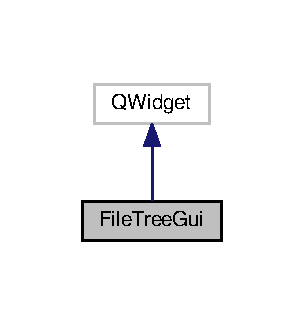
\includegraphics[width=146pt]{class_file_tree_gui__inherit__graph}
\end{center}
\end{figure}


Collaboration diagram for File\-Tree\-Gui\-:\nopagebreak
\begin{figure}[H]
\begin{center}
\leavevmode
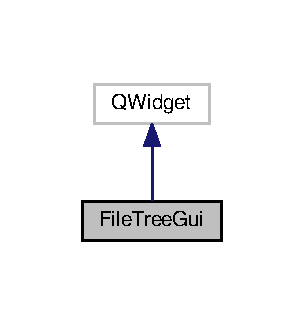
\includegraphics[width=146pt]{class_file_tree_gui__coll__graph}
\end{center}
\end{figure}
\subsection*{Public Member Functions}
\begin{DoxyCompactItemize}
\item 
\hyperlink{class_file_tree_gui_acf857f2793adefb176a680d541c24691}{File\-Tree\-Gui} (Q\-Widget $\ast$parent=0)
\item 
void \hyperlink{class_file_tree_gui_a571ca6424f269c0035ae9ddbce2e9e60}{set\-Master\-Tab\-Widget\-Ptr} (Q\-Tab\-Widget $\ast$\hyperlink{class_file_tree_gui_adb1e3ecfaab582317fcd9b968bbf6c40}{master\-Tab\-Widget\-Ptr})
\item 
Q\-Tab\-Widget $\ast$ \hyperlink{class_file_tree_gui_ab4c244617e4a8fbc13608cf5cfcf6944}{get\-Master\-Tab\-Widget\-Ptr} ()
\item 
\hyperlink{class_file_tree_gui_a11cc4baa3a62a625e95155c27a0d7258}{$\sim$\-File\-Tree\-Gui} ()
\end{DoxyCompactItemize}
\subsection*{Static Public Member Functions}
\begin{DoxyCompactItemize}
\item 
static void \hyperlink{class_file_tree_gui_a5d4df4a19da0183ccc254019f77097b1}{init\-Tree} ()
\item 
static void \hyperlink{class_file_tree_gui_ab3c2fd5311245c08624461ac4c7e120c}{add\-Children} (Q\-Tree\-Widget\-Item $\ast$item, Q\-String file\-Path)
\item 
static void \hyperlink{class_file_tree_gui_afe882583424429fcda9c4c2bc0ab71d4}{set\-Project\-Root\-Abs\-Path\-Str\-Ptr} (Q\-String $\ast$\hyperlink{class_file_tree_gui_a9ce991f8f95f583aa5fb1bec7a9bcd4c}{project\-Root\-Abs\-Path\-Str\-Ptr})
\item 
static Q\-String $\ast$ \hyperlink{class_file_tree_gui_a21607e8cda6732997d5148581017a9b8}{get\-Project\-Root\-Abs\-Path\-Str\-Ptr} ()
\item 
static void \hyperlink{class_file_tree_gui_ac2c3399b5cb85da5cd1c119b61c674c0}{refresh} ()
\end{DoxyCompactItemize}
\subsection*{Private Slots}
\begin{DoxyCompactItemize}
\item 
void \hyperlink{class_file_tree_gui_aa8110a99d6bab64818b7f87024382b2a}{handle\-Show\-Directory\-Slot} (Q\-Tree\-Widget\-Item $\ast$item, int)
\item 
void \hyperlink{class_file_tree_gui_a9d726b5258284de8f9dc10cddddbdc87}{handle\-Right\-Click\-Slot} (const Q\-Point \&)
\end{DoxyCompactItemize}
\subsection*{Private Attributes}
\begin{DoxyCompactItemize}
\item 
Q\-Grid\-Layout $\ast$ \hyperlink{class_file_tree_gui_aaf8b63a4775b1d46d635cdaef94b979a}{outer\-Layout}
\item 
Q\-Tab\-Widget $\ast$ \hyperlink{class_file_tree_gui_adb1e3ecfaab582317fcd9b968bbf6c40}{master\-Tab\-Widget\-Ptr}
\end{DoxyCompactItemize}
\subsection*{Static Private Attributes}
\begin{DoxyCompactItemize}
\item 
static Q\-Tree\-Widget $\ast$ \hyperlink{class_file_tree_gui_a27648a2d00b8283605c3a260060b1285}{true\-Tree}
\item 
static Q\-Splitter $\ast$ \hyperlink{class_file_tree_gui_a43e8677ba8c50059d003f298b631e131}{splitter}
\item 
static Q\-String $\ast$ \hyperlink{class_file_tree_gui_a9ce991f8f95f583aa5fb1bec7a9bcd4c}{project\-Root\-Abs\-Path\-Str\-Ptr}
\end{DoxyCompactItemize}


\subsection{Detailed Description}


Definition at line 35 of file File\-Tree\-Gui.\-h.



\subsection{Constructor \& Destructor Documentation}
\hypertarget{class_file_tree_gui_acf857f2793adefb176a680d541c24691}{\index{File\-Tree\-Gui@{File\-Tree\-Gui}!File\-Tree\-Gui@{File\-Tree\-Gui}}
\index{File\-Tree\-Gui@{File\-Tree\-Gui}!FileTreeGui@{File\-Tree\-Gui}}
\subsubsection[{File\-Tree\-Gui}]{\setlength{\rightskip}{0pt plus 5cm}File\-Tree\-Gui\-::\-File\-Tree\-Gui (
\begin{DoxyParamCaption}
\item[{Q\-Widget $\ast$}]{parent = {\ttfamily 0}}
\end{DoxyParamCaption}
)}}\label{class_file_tree_gui_acf857f2793adefb176a680d541c24691}


Definition at line 10 of file File\-Tree\-Gui.\-cpp.

\hypertarget{class_file_tree_gui_a11cc4baa3a62a625e95155c27a0d7258}{\index{File\-Tree\-Gui@{File\-Tree\-Gui}!$\sim$\-File\-Tree\-Gui@{$\sim$\-File\-Tree\-Gui}}
\index{$\sim$\-File\-Tree\-Gui@{$\sim$\-File\-Tree\-Gui}!FileTreeGui@{File\-Tree\-Gui}}
\subsubsection[{$\sim$\-File\-Tree\-Gui}]{\setlength{\rightskip}{0pt plus 5cm}File\-Tree\-Gui\-::$\sim$\-File\-Tree\-Gui (
\begin{DoxyParamCaption}
{}
\end{DoxyParamCaption}
)}}\label{class_file_tree_gui_a11cc4baa3a62a625e95155c27a0d7258}


Definition at line 200 of file File\-Tree\-Gui.\-cpp.



\subsection{Member Function Documentation}
\hypertarget{class_file_tree_gui_ab3c2fd5311245c08624461ac4c7e120c}{\index{File\-Tree\-Gui@{File\-Tree\-Gui}!add\-Children@{add\-Children}}
\index{add\-Children@{add\-Children}!FileTreeGui@{File\-Tree\-Gui}}
\subsubsection[{add\-Children}]{\setlength{\rightskip}{0pt plus 5cm}void File\-Tree\-Gui\-::add\-Children (
\begin{DoxyParamCaption}
\item[{Q\-Tree\-Widget\-Item $\ast$}]{item, }
\item[{Q\-String}]{file\-Path}
\end{DoxyParamCaption}
)\hspace{0.3cm}{\ttfamily [static]}}}\label{class_file_tree_gui_ab3c2fd5311245c08624461ac4c7e120c}


Definition at line 72 of file File\-Tree\-Gui.\-cpp.

\hypertarget{class_file_tree_gui_ab4c244617e4a8fbc13608cf5cfcf6944}{\index{File\-Tree\-Gui@{File\-Tree\-Gui}!get\-Master\-Tab\-Widget\-Ptr@{get\-Master\-Tab\-Widget\-Ptr}}
\index{get\-Master\-Tab\-Widget\-Ptr@{get\-Master\-Tab\-Widget\-Ptr}!FileTreeGui@{File\-Tree\-Gui}}
\subsubsection[{get\-Master\-Tab\-Widget\-Ptr}]{\setlength{\rightskip}{0pt plus 5cm}Q\-Tab\-Widget $\ast$ File\-Tree\-Gui\-::get\-Master\-Tab\-Widget\-Ptr (
\begin{DoxyParamCaption}
{}
\end{DoxyParamCaption}
)}}\label{class_file_tree_gui_ab4c244617e4a8fbc13608cf5cfcf6944}


Definition at line 194 of file File\-Tree\-Gui.\-cpp.

\hypertarget{class_file_tree_gui_a21607e8cda6732997d5148581017a9b8}{\index{File\-Tree\-Gui@{File\-Tree\-Gui}!get\-Project\-Root\-Abs\-Path\-Str\-Ptr@{get\-Project\-Root\-Abs\-Path\-Str\-Ptr}}
\index{get\-Project\-Root\-Abs\-Path\-Str\-Ptr@{get\-Project\-Root\-Abs\-Path\-Str\-Ptr}!FileTreeGui@{File\-Tree\-Gui}}
\subsubsection[{get\-Project\-Root\-Abs\-Path\-Str\-Ptr}]{\setlength{\rightskip}{0pt plus 5cm}Q\-String $\ast$ File\-Tree\-Gui\-::get\-Project\-Root\-Abs\-Path\-Str\-Ptr (
\begin{DoxyParamCaption}
{}
\end{DoxyParamCaption}
)\hspace{0.3cm}{\ttfamily [static]}}}\label{class_file_tree_gui_a21607e8cda6732997d5148581017a9b8}


Definition at line 172 of file File\-Tree\-Gui.\-cpp.

\hypertarget{class_file_tree_gui_a9d726b5258284de8f9dc10cddddbdc87}{\index{File\-Tree\-Gui@{File\-Tree\-Gui}!handle\-Right\-Click\-Slot@{handle\-Right\-Click\-Slot}}
\index{handle\-Right\-Click\-Slot@{handle\-Right\-Click\-Slot}!FileTreeGui@{File\-Tree\-Gui}}
\subsubsection[{handle\-Right\-Click\-Slot}]{\setlength{\rightskip}{0pt plus 5cm}void File\-Tree\-Gui\-::handle\-Right\-Click\-Slot (
\begin{DoxyParamCaption}
\item[{const Q\-Point \&}]{pos}
\end{DoxyParamCaption}
)\hspace{0.3cm}{\ttfamily [private]}, {\ttfamily [slot]}}}\label{class_file_tree_gui_a9d726b5258284de8f9dc10cddddbdc87}


Definition at line 135 of file File\-Tree\-Gui.\-cpp.

\hypertarget{class_file_tree_gui_aa8110a99d6bab64818b7f87024382b2a}{\index{File\-Tree\-Gui@{File\-Tree\-Gui}!handle\-Show\-Directory\-Slot@{handle\-Show\-Directory\-Slot}}
\index{handle\-Show\-Directory\-Slot@{handle\-Show\-Directory\-Slot}!FileTreeGui@{File\-Tree\-Gui}}
\subsubsection[{handle\-Show\-Directory\-Slot}]{\setlength{\rightskip}{0pt plus 5cm}void File\-Tree\-Gui\-::handle\-Show\-Directory\-Slot (
\begin{DoxyParamCaption}
\item[{Q\-Tree\-Widget\-Item $\ast$}]{item, }
\item[{int}]{column}
\end{DoxyParamCaption}
)\hspace{0.3cm}{\ttfamily [private]}, {\ttfamily [slot]}}}\label{class_file_tree_gui_aa8110a99d6bab64818b7f87024382b2a}


Definition at line 99 of file File\-Tree\-Gui.\-cpp.

\hypertarget{class_file_tree_gui_a5d4df4a19da0183ccc254019f77097b1}{\index{File\-Tree\-Gui@{File\-Tree\-Gui}!init\-Tree@{init\-Tree}}
\index{init\-Tree@{init\-Tree}!FileTreeGui@{File\-Tree\-Gui}}
\subsubsection[{init\-Tree}]{\setlength{\rightskip}{0pt plus 5cm}void File\-Tree\-Gui\-::init\-Tree (
\begin{DoxyParamCaption}
{}
\end{DoxyParamCaption}
)\hspace{0.3cm}{\ttfamily [static]}}}\label{class_file_tree_gui_a5d4df4a19da0183ccc254019f77097b1}


Definition at line 40 of file File\-Tree\-Gui.\-cpp.

\hypertarget{class_file_tree_gui_ac2c3399b5cb85da5cd1c119b61c674c0}{\index{File\-Tree\-Gui@{File\-Tree\-Gui}!refresh@{refresh}}
\index{refresh@{refresh}!FileTreeGui@{File\-Tree\-Gui}}
\subsubsection[{refresh}]{\setlength{\rightskip}{0pt plus 5cm}void File\-Tree\-Gui\-::refresh (
\begin{DoxyParamCaption}
{}
\end{DoxyParamCaption}
)\hspace{0.3cm}{\ttfamily [static]}}}\label{class_file_tree_gui_ac2c3399b5cb85da5cd1c119b61c674c0}


Definition at line 178 of file File\-Tree\-Gui.\-cpp.

\hypertarget{class_file_tree_gui_a571ca6424f269c0035ae9ddbce2e9e60}{\index{File\-Tree\-Gui@{File\-Tree\-Gui}!set\-Master\-Tab\-Widget\-Ptr@{set\-Master\-Tab\-Widget\-Ptr}}
\index{set\-Master\-Tab\-Widget\-Ptr@{set\-Master\-Tab\-Widget\-Ptr}!FileTreeGui@{File\-Tree\-Gui}}
\subsubsection[{set\-Master\-Tab\-Widget\-Ptr}]{\setlength{\rightskip}{0pt plus 5cm}void File\-Tree\-Gui\-::set\-Master\-Tab\-Widget\-Ptr (
\begin{DoxyParamCaption}
\item[{Q\-Tab\-Widget $\ast$}]{master\-Tab\-Widget\-Ptr}
\end{DoxyParamCaption}
)}}\label{class_file_tree_gui_a571ca6424f269c0035ae9ddbce2e9e60}


Definition at line 188 of file File\-Tree\-Gui.\-cpp.

\hypertarget{class_file_tree_gui_afe882583424429fcda9c4c2bc0ab71d4}{\index{File\-Tree\-Gui@{File\-Tree\-Gui}!set\-Project\-Root\-Abs\-Path\-Str\-Ptr@{set\-Project\-Root\-Abs\-Path\-Str\-Ptr}}
\index{set\-Project\-Root\-Abs\-Path\-Str\-Ptr@{set\-Project\-Root\-Abs\-Path\-Str\-Ptr}!FileTreeGui@{File\-Tree\-Gui}}
\subsubsection[{set\-Project\-Root\-Abs\-Path\-Str\-Ptr}]{\setlength{\rightskip}{0pt plus 5cm}void File\-Tree\-Gui\-::set\-Project\-Root\-Abs\-Path\-Str\-Ptr (
\begin{DoxyParamCaption}
\item[{Q\-String $\ast$}]{project\-Root\-Abs\-Path\-Str\-Ptr}
\end{DoxyParamCaption}
)\hspace{0.3cm}{\ttfamily [static]}}}\label{class_file_tree_gui_afe882583424429fcda9c4c2bc0ab71d4}


Definition at line 166 of file File\-Tree\-Gui.\-cpp.



\subsection{Member Data Documentation}
\hypertarget{class_file_tree_gui_adb1e3ecfaab582317fcd9b968bbf6c40}{\index{File\-Tree\-Gui@{File\-Tree\-Gui}!master\-Tab\-Widget\-Ptr@{master\-Tab\-Widget\-Ptr}}
\index{master\-Tab\-Widget\-Ptr@{master\-Tab\-Widget\-Ptr}!FileTreeGui@{File\-Tree\-Gui}}
\subsubsection[{master\-Tab\-Widget\-Ptr}]{\setlength{\rightskip}{0pt plus 5cm}Q\-Tab\-Widget$\ast$ File\-Tree\-Gui\-::master\-Tab\-Widget\-Ptr\hspace{0.3cm}{\ttfamily [private]}}}\label{class_file_tree_gui_adb1e3ecfaab582317fcd9b968bbf6c40}


Definition at line 46 of file File\-Tree\-Gui.\-h.

\hypertarget{class_file_tree_gui_aaf8b63a4775b1d46d635cdaef94b979a}{\index{File\-Tree\-Gui@{File\-Tree\-Gui}!outer\-Layout@{outer\-Layout}}
\index{outer\-Layout@{outer\-Layout}!FileTreeGui@{File\-Tree\-Gui}}
\subsubsection[{outer\-Layout}]{\setlength{\rightskip}{0pt plus 5cm}Q\-Grid\-Layout$\ast$ File\-Tree\-Gui\-::outer\-Layout\hspace{0.3cm}{\ttfamily [private]}}}\label{class_file_tree_gui_aaf8b63a4775b1d46d635cdaef94b979a}


Definition at line 43 of file File\-Tree\-Gui.\-h.

\hypertarget{class_file_tree_gui_a9ce991f8f95f583aa5fb1bec7a9bcd4c}{\index{File\-Tree\-Gui@{File\-Tree\-Gui}!project\-Root\-Abs\-Path\-Str\-Ptr@{project\-Root\-Abs\-Path\-Str\-Ptr}}
\index{project\-Root\-Abs\-Path\-Str\-Ptr@{project\-Root\-Abs\-Path\-Str\-Ptr}!FileTreeGui@{File\-Tree\-Gui}}
\subsubsection[{project\-Root\-Abs\-Path\-Str\-Ptr}]{\setlength{\rightskip}{0pt plus 5cm}Q\-String $\ast$ File\-Tree\-Gui\-::project\-Root\-Abs\-Path\-Str\-Ptr\hspace{0.3cm}{\ttfamily [static]}, {\ttfamily [private]}}}\label{class_file_tree_gui_a9ce991f8f95f583aa5fb1bec7a9bcd4c}


Definition at line 45 of file File\-Tree\-Gui.\-h.

\hypertarget{class_file_tree_gui_a43e8677ba8c50059d003f298b631e131}{\index{File\-Tree\-Gui@{File\-Tree\-Gui}!splitter@{splitter}}
\index{splitter@{splitter}!FileTreeGui@{File\-Tree\-Gui}}
\subsubsection[{splitter}]{\setlength{\rightskip}{0pt plus 5cm}Q\-Splitter $\ast$ File\-Tree\-Gui\-::splitter\hspace{0.3cm}{\ttfamily [static]}, {\ttfamily [private]}}}\label{class_file_tree_gui_a43e8677ba8c50059d003f298b631e131}


Definition at line 41 of file File\-Tree\-Gui.\-h.

\hypertarget{class_file_tree_gui_a27648a2d00b8283605c3a260060b1285}{\index{File\-Tree\-Gui@{File\-Tree\-Gui}!true\-Tree@{true\-Tree}}
\index{true\-Tree@{true\-Tree}!FileTreeGui@{File\-Tree\-Gui}}
\subsubsection[{true\-Tree}]{\setlength{\rightskip}{0pt plus 5cm}Q\-Tree\-Widget $\ast$ File\-Tree\-Gui\-::true\-Tree\hspace{0.3cm}{\ttfamily [static]}, {\ttfamily [private]}}}\label{class_file_tree_gui_a27648a2d00b8283605c3a260060b1285}


Definition at line 40 of file File\-Tree\-Gui.\-h.



The documentation for this class was generated from the following files\-:\begin{DoxyCompactItemize}
\item 
/home/james/\-Net\-Beans\-Projects/ride/src/\hyperlink{_file_tree_gui_8h}{File\-Tree\-Gui.\-h}\item 
/home/james/\-Net\-Beans\-Projects/ride/src/\hyperlink{_file_tree_gui_8cpp}{File\-Tree\-Gui.\-cpp}\end{DoxyCompactItemize}

\hypertarget{class_highlighter}{\section{Highlighter Class Reference}
\label{class_highlighter}\index{Highlighter@{Highlighter}}
}


{\ttfamily \#include $<$Highlighter.\-h$>$}



Inheritance diagram for Highlighter\-:\nopagebreak
\begin{figure}[H]
\begin{center}
\leavevmode
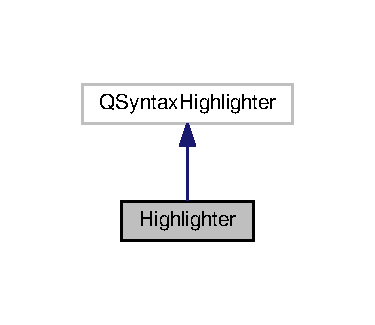
\includegraphics[width=180pt]{class_highlighter__inherit__graph}
\end{center}
\end{figure}


Collaboration diagram for Highlighter\-:\nopagebreak
\begin{figure}[H]
\begin{center}
\leavevmode
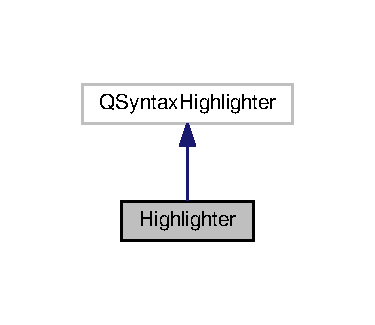
\includegraphics[width=180pt]{class_highlighter__coll__graph}
\end{center}
\end{figure}
\subsection*{Classes}
\begin{DoxyCompactItemize}
\item 
struct \hyperlink{struct_highlighter_1_1_highlighting_rule}{Highlighting\-Rule}
\end{DoxyCompactItemize}
\subsection*{Public Member Functions}
\begin{DoxyCompactItemize}
\item 
\hyperlink{class_highlighter_af9fa54a58a9365e91e5f8eccf22f5153}{Highlighter} (Q\-Text\-Document $\ast$parent=0)
\end{DoxyCompactItemize}
\subsection*{Protected Member Functions}
\begin{DoxyCompactItemize}
\item 
void \hyperlink{class_highlighter_ad07c7fd55d2ce2c675bca607b9370488}{highlight\-Block} (const Q\-String \&text)
\end{DoxyCompactItemize}
\subsection*{Private Attributes}
\begin{DoxyCompactItemize}
\item 
Q\-Vector$<$ \hyperlink{struct_highlighter_1_1_highlighting_rule}{Highlighting\-Rule} $>$ \hyperlink{class_highlighter_aa23f8b3f4ddd1354f508b46d77897fe5}{highlighting\-Rules}
\item 
Q\-Reg\-Exp \hyperlink{class_highlighter_a67cdecd667929b4eefbc7057d58cd90b}{comment\-Start\-Expression}
\item 
Q\-Reg\-Exp \hyperlink{class_highlighter_a3baa1033bbdf70a16df42940968b72b4}{comment\-End\-Expression}
\item 
Q\-Text\-Char\-Format \hyperlink{class_highlighter_acf807339a8cd02097a81e455ef2686d2}{keyword\-Format}
\item 
Q\-Text\-Char\-Format \hyperlink{class_highlighter_a765a13081aa25d818c766b7f8e50f454}{class\-Format}
\item 
Q\-Text\-Char\-Format \hyperlink{class_highlighter_ad1ca0f6942b0451781d7e32f1781f22b}{single\-Line\-Comment\-Format}
\item 
Q\-Text\-Char\-Format \hyperlink{class_highlighter_ad4661760f22cf913b696ec90dea994c0}{multi\-Line\-Comment\-Format}
\item 
Q\-Text\-Char\-Format \hyperlink{class_highlighter_a3d4bf96c8ea27ba18bca4adc6b306db8}{quotation\-Format}
\item 
Q\-Text\-Char\-Format \hyperlink{class_highlighter_a7e02cd8caee678c1256998c88d30e241}{function\-Format}
\end{DoxyCompactItemize}


\subsection{Detailed Description}


Definition at line 22 of file Highlighter.\-h.



\subsection{Constructor \& Destructor Documentation}
\hypertarget{class_highlighter_af9fa54a58a9365e91e5f8eccf22f5153}{\index{Highlighter@{Highlighter}!Highlighter@{Highlighter}}
\index{Highlighter@{Highlighter}!Highlighter@{Highlighter}}
\subsubsection[{Highlighter}]{\setlength{\rightskip}{0pt plus 5cm}Highlighter\-::\-Highlighter (
\begin{DoxyParamCaption}
\item[{Q\-Text\-Document $\ast$}]{parent = {\ttfamily 0}}
\end{DoxyParamCaption}
)}}\label{class_highlighter_af9fa54a58a9365e91e5f8eccf22f5153}


Definition at line 3 of file Highlighter.\-cpp.



Here is the call graph for this function\-:
\nopagebreak
\begin{figure}[H]
\begin{center}
\leavevmode
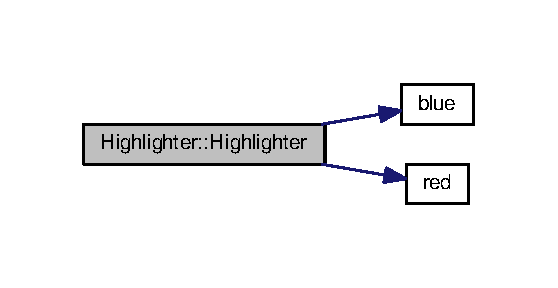
\includegraphics[width=268pt]{class_highlighter_af9fa54a58a9365e91e5f8eccf22f5153_cgraph}
\end{center}
\end{figure}




\subsection{Member Function Documentation}
\hypertarget{class_highlighter_ad07c7fd55d2ce2c675bca607b9370488}{\index{Highlighter@{Highlighter}!highlight\-Block@{highlight\-Block}}
\index{highlight\-Block@{highlight\-Block}!Highlighter@{Highlighter}}
\subsubsection[{highlight\-Block}]{\setlength{\rightskip}{0pt plus 5cm}void Highlighter\-::highlight\-Block (
\begin{DoxyParamCaption}
\item[{const Q\-String \&}]{text}
\end{DoxyParamCaption}
)\hspace{0.3cm}{\ttfamily [protected]}}}\label{class_highlighter_ad07c7fd55d2ce2c675bca607b9370488}


Definition at line 158 of file Highlighter.\-cpp.



\subsection{Member Data Documentation}
\hypertarget{class_highlighter_a765a13081aa25d818c766b7f8e50f454}{\index{Highlighter@{Highlighter}!class\-Format@{class\-Format}}
\index{class\-Format@{class\-Format}!Highlighter@{Highlighter}}
\subsubsection[{class\-Format}]{\setlength{\rightskip}{0pt plus 5cm}Q\-Text\-Char\-Format Highlighter\-::class\-Format\hspace{0.3cm}{\ttfamily [private]}}}\label{class_highlighter_a765a13081aa25d818c766b7f8e50f454}


Definition at line 38 of file Highlighter.\-h.

\hypertarget{class_highlighter_a3baa1033bbdf70a16df42940968b72b4}{\index{Highlighter@{Highlighter}!comment\-End\-Expression@{comment\-End\-Expression}}
\index{comment\-End\-Expression@{comment\-End\-Expression}!Highlighter@{Highlighter}}
\subsubsection[{comment\-End\-Expression}]{\setlength{\rightskip}{0pt plus 5cm}Q\-Reg\-Exp Highlighter\-::comment\-End\-Expression\hspace{0.3cm}{\ttfamily [private]}}}\label{class_highlighter_a3baa1033bbdf70a16df42940968b72b4}


Definition at line 35 of file Highlighter.\-h.

\hypertarget{class_highlighter_a67cdecd667929b4eefbc7057d58cd90b}{\index{Highlighter@{Highlighter}!comment\-Start\-Expression@{comment\-Start\-Expression}}
\index{comment\-Start\-Expression@{comment\-Start\-Expression}!Highlighter@{Highlighter}}
\subsubsection[{comment\-Start\-Expression}]{\setlength{\rightskip}{0pt plus 5cm}Q\-Reg\-Exp Highlighter\-::comment\-Start\-Expression\hspace{0.3cm}{\ttfamily [private]}}}\label{class_highlighter_a67cdecd667929b4eefbc7057d58cd90b}


Definition at line 34 of file Highlighter.\-h.

\hypertarget{class_highlighter_a7e02cd8caee678c1256998c88d30e241}{\index{Highlighter@{Highlighter}!function\-Format@{function\-Format}}
\index{function\-Format@{function\-Format}!Highlighter@{Highlighter}}
\subsubsection[{function\-Format}]{\setlength{\rightskip}{0pt plus 5cm}Q\-Text\-Char\-Format Highlighter\-::function\-Format\hspace{0.3cm}{\ttfamily [private]}}}\label{class_highlighter_a7e02cd8caee678c1256998c88d30e241}


Definition at line 42 of file Highlighter.\-h.

\hypertarget{class_highlighter_aa23f8b3f4ddd1354f508b46d77897fe5}{\index{Highlighter@{Highlighter}!highlighting\-Rules@{highlighting\-Rules}}
\index{highlighting\-Rules@{highlighting\-Rules}!Highlighter@{Highlighter}}
\subsubsection[{highlighting\-Rules}]{\setlength{\rightskip}{0pt plus 5cm}Q\-Vector$<${\bf Highlighting\-Rule}$>$ Highlighter\-::highlighting\-Rules\hspace{0.3cm}{\ttfamily [private]}}}\label{class_highlighter_aa23f8b3f4ddd1354f508b46d77897fe5}


Definition at line 32 of file Highlighter.\-h.

\hypertarget{class_highlighter_acf807339a8cd02097a81e455ef2686d2}{\index{Highlighter@{Highlighter}!keyword\-Format@{keyword\-Format}}
\index{keyword\-Format@{keyword\-Format}!Highlighter@{Highlighter}}
\subsubsection[{keyword\-Format}]{\setlength{\rightskip}{0pt plus 5cm}Q\-Text\-Char\-Format Highlighter\-::keyword\-Format\hspace{0.3cm}{\ttfamily [private]}}}\label{class_highlighter_acf807339a8cd02097a81e455ef2686d2}


Definition at line 37 of file Highlighter.\-h.

\hypertarget{class_highlighter_ad4661760f22cf913b696ec90dea994c0}{\index{Highlighter@{Highlighter}!multi\-Line\-Comment\-Format@{multi\-Line\-Comment\-Format}}
\index{multi\-Line\-Comment\-Format@{multi\-Line\-Comment\-Format}!Highlighter@{Highlighter}}
\subsubsection[{multi\-Line\-Comment\-Format}]{\setlength{\rightskip}{0pt plus 5cm}Q\-Text\-Char\-Format Highlighter\-::multi\-Line\-Comment\-Format\hspace{0.3cm}{\ttfamily [private]}}}\label{class_highlighter_ad4661760f22cf913b696ec90dea994c0}


Definition at line 40 of file Highlighter.\-h.

\hypertarget{class_highlighter_a3d4bf96c8ea27ba18bca4adc6b306db8}{\index{Highlighter@{Highlighter}!quotation\-Format@{quotation\-Format}}
\index{quotation\-Format@{quotation\-Format}!Highlighter@{Highlighter}}
\subsubsection[{quotation\-Format}]{\setlength{\rightskip}{0pt plus 5cm}Q\-Text\-Char\-Format Highlighter\-::quotation\-Format\hspace{0.3cm}{\ttfamily [private]}}}\label{class_highlighter_a3d4bf96c8ea27ba18bca4adc6b306db8}


Definition at line 41 of file Highlighter.\-h.

\hypertarget{class_highlighter_ad1ca0f6942b0451781d7e32f1781f22b}{\index{Highlighter@{Highlighter}!single\-Line\-Comment\-Format@{single\-Line\-Comment\-Format}}
\index{single\-Line\-Comment\-Format@{single\-Line\-Comment\-Format}!Highlighter@{Highlighter}}
\subsubsection[{single\-Line\-Comment\-Format}]{\setlength{\rightskip}{0pt plus 5cm}Q\-Text\-Char\-Format Highlighter\-::single\-Line\-Comment\-Format\hspace{0.3cm}{\ttfamily [private]}}}\label{class_highlighter_ad1ca0f6942b0451781d7e32f1781f22b}


Definition at line 39 of file Highlighter.\-h.



The documentation for this class was generated from the following files\-:\begin{DoxyCompactItemize}
\item 
/home/james/\-Net\-Beans\-Projects/ride/src/\hyperlink{_highlighter_8h}{Highlighter.\-h}\item 
/home/james/\-Net\-Beans\-Projects/ride/src/\hyperlink{_highlighter_8cpp}{Highlighter.\-cpp}\end{DoxyCompactItemize}

\hypertarget{struct_highlighter_1_1_highlighting_rule}{\section{Highlighter\-:\-:Highlighting\-Rule Struct Reference}
\label{struct_highlighter_1_1_highlighting_rule}\index{Highlighter\-::\-Highlighting\-Rule@{Highlighter\-::\-Highlighting\-Rule}}
}
\subsection*{Public Attributes}
\begin{DoxyCompactItemize}
\item 
Q\-Reg\-Exp \hyperlink{struct_highlighter_1_1_highlighting_rule_aaecab525cb637802e0c4a10e8832cd84}{pattern}
\item 
Q\-Text\-Char\-Format \hyperlink{struct_highlighter_1_1_highlighting_rule_ae0a636ba88b740accc9b98ca777b6fb4}{format}
\end{DoxyCompactItemize}


\subsection{Detailed Description}


Definition at line 23 of file Highlighter.\-h.



\subsection{Member Data Documentation}
\hypertarget{struct_highlighter_1_1_highlighting_rule_ae0a636ba88b740accc9b98ca777b6fb4}{\index{Highlighter\-::\-Highlighting\-Rule@{Highlighter\-::\-Highlighting\-Rule}!format@{format}}
\index{format@{format}!Highlighter::HighlightingRule@{Highlighter\-::\-Highlighting\-Rule}}
\subsubsection[{format}]{\setlength{\rightskip}{0pt plus 5cm}Q\-Text\-Char\-Format Highlighter\-::\-Highlighting\-Rule\-::format}}\label{struct_highlighter_1_1_highlighting_rule_ae0a636ba88b740accc9b98ca777b6fb4}


Definition at line 26 of file Highlighter.\-h.

\hypertarget{struct_highlighter_1_1_highlighting_rule_aaecab525cb637802e0c4a10e8832cd84}{\index{Highlighter\-::\-Highlighting\-Rule@{Highlighter\-::\-Highlighting\-Rule}!pattern@{pattern}}
\index{pattern@{pattern}!Highlighter::HighlightingRule@{Highlighter\-::\-Highlighting\-Rule}}
\subsubsection[{pattern}]{\setlength{\rightskip}{0pt plus 5cm}Q\-Reg\-Exp Highlighter\-::\-Highlighting\-Rule\-::pattern}}\label{struct_highlighter_1_1_highlighting_rule_aaecab525cb637802e0c4a10e8832cd84}


Definition at line 25 of file Highlighter.\-h.



The documentation for this struct was generated from the following file\-:\begin{DoxyCompactItemize}
\item 
/home/james/\-Net\-Beans\-Projects/ride/src/\hyperlink{_highlighter_8h}{Highlighter.\-h}\end{DoxyCompactItemize}

\hypertarget{class_line_number_area}{\section{Line\-Number\-Area Class Reference}
\label{class_line_number_area}\index{Line\-Number\-Area@{Line\-Number\-Area}}
}


{\ttfamily \#include $<$Line\-Number\-Area.\-h$>$}



Inheritance diagram for Line\-Number\-Area\-:\nopagebreak
\begin{figure}[H]
\begin{center}
\leavevmode
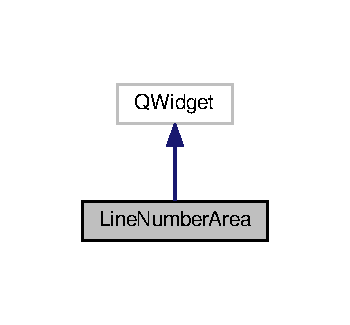
\includegraphics[width=168pt]{class_line_number_area__inherit__graph}
\end{center}
\end{figure}


Collaboration diagram for Line\-Number\-Area\-:\nopagebreak
\begin{figure}[H]
\begin{center}
\leavevmode
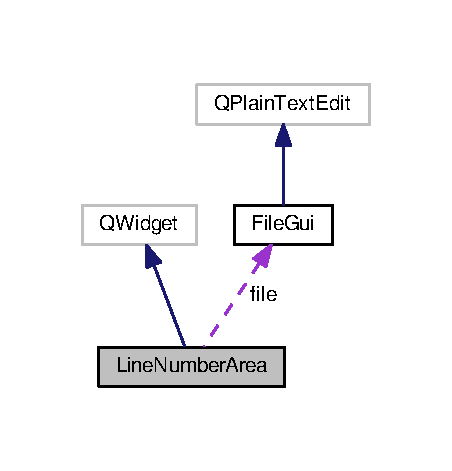
\includegraphics[width=217pt]{class_line_number_area__coll__graph}
\end{center}
\end{figure}
\subsection*{Public Member Functions}
\begin{DoxyCompactItemize}
\item 
\hyperlink{class_line_number_area_a7bc91f89287a239f287915c96537a5fc}{Line\-Number\-Area} (\hyperlink{class_file_gui}{File\-Gui} $\ast$parent=0)
\item 
Q\-Size \hyperlink{class_line_number_area_a5d31f7fb107bc1eefd7ae4974c095308}{size\-Hint} () const 
\item 
void \hyperlink{class_line_number_area_a56400934bfe272427deb3ffd975b3a7f}{paint\-Event} (Q\-Paint\-Event $\ast$event)
\item 
\hyperlink{class_line_number_area_abccdc5ad204da18e0fedee62ad4a58ce}{$\sim$\-Line\-Number\-Area} ()
\end{DoxyCompactItemize}
\subsection*{Private Attributes}
\begin{DoxyCompactItemize}
\item 
\hyperlink{class_file_gui}{File\-Gui} $\ast$ \hyperlink{class_line_number_area_a08ebbed0dba5e4740c0af7d006614922}{file}
\end{DoxyCompactItemize}


\subsection{Detailed Description}


Definition at line 17 of file Line\-Number\-Area.\-h.



\subsection{Constructor \& Destructor Documentation}
\hypertarget{class_line_number_area_a7bc91f89287a239f287915c96537a5fc}{\index{Line\-Number\-Area@{Line\-Number\-Area}!Line\-Number\-Area@{Line\-Number\-Area}}
\index{Line\-Number\-Area@{Line\-Number\-Area}!LineNumberArea@{Line\-Number\-Area}}
\subsubsection[{Line\-Number\-Area}]{\setlength{\rightskip}{0pt plus 5cm}Line\-Number\-Area\-::\-Line\-Number\-Area (
\begin{DoxyParamCaption}
\item[{{\bf File\-Gui} $\ast$}]{parent = {\ttfamily 0}}
\end{DoxyParamCaption}
)}}\label{class_line_number_area_a7bc91f89287a239f287915c96537a5fc}


Definition at line 48 of file Line\-Number\-Area.\-cpp.

\hypertarget{class_line_number_area_abccdc5ad204da18e0fedee62ad4a58ce}{\index{Line\-Number\-Area@{Line\-Number\-Area}!$\sim$\-Line\-Number\-Area@{$\sim$\-Line\-Number\-Area}}
\index{$\sim$\-Line\-Number\-Area@{$\sim$\-Line\-Number\-Area}!LineNumberArea@{Line\-Number\-Area}}
\subsubsection[{$\sim$\-Line\-Number\-Area}]{\setlength{\rightskip}{0pt plus 5cm}Line\-Number\-Area\-::$\sim$\-Line\-Number\-Area (
\begin{DoxyParamCaption}
{}
\end{DoxyParamCaption}
)}}\label{class_line_number_area_abccdc5ad204da18e0fedee62ad4a58ce}


Definition at line 65 of file Line\-Number\-Area.\-cpp.



\subsection{Member Function Documentation}
\hypertarget{class_line_number_area_a56400934bfe272427deb3ffd975b3a7f}{\index{Line\-Number\-Area@{Line\-Number\-Area}!paint\-Event@{paint\-Event}}
\index{paint\-Event@{paint\-Event}!LineNumberArea@{Line\-Number\-Area}}
\subsubsection[{paint\-Event}]{\setlength{\rightskip}{0pt plus 5cm}void Line\-Number\-Area\-::paint\-Event (
\begin{DoxyParamCaption}
\item[{Q\-Paint\-Event $\ast$}]{event}
\end{DoxyParamCaption}
)}}\label{class_line_number_area_a56400934bfe272427deb3ffd975b3a7f}


Definition at line 59 of file Line\-Number\-Area.\-cpp.



Here is the call graph for this function\-:
\nopagebreak
\begin{figure}[H]
\begin{center}
\leavevmode
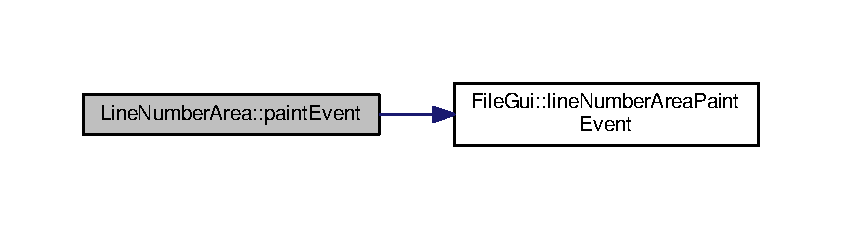
\includegraphics[width=350pt]{class_line_number_area_a56400934bfe272427deb3ffd975b3a7f_cgraph}
\end{center}
\end{figure}


\hypertarget{class_line_number_area_a5d31f7fb107bc1eefd7ae4974c095308}{\index{Line\-Number\-Area@{Line\-Number\-Area}!size\-Hint@{size\-Hint}}
\index{size\-Hint@{size\-Hint}!LineNumberArea@{Line\-Number\-Area}}
\subsubsection[{size\-Hint}]{\setlength{\rightskip}{0pt plus 5cm}Q\-Size Line\-Number\-Area\-::size\-Hint (
\begin{DoxyParamCaption}
{}
\end{DoxyParamCaption}
) const}}\label{class_line_number_area_a5d31f7fb107bc1eefd7ae4974c095308}


Definition at line 54 of file Line\-Number\-Area.\-cpp.



Here is the call graph for this function\-:
\nopagebreak
\begin{figure}[H]
\begin{center}
\leavevmode
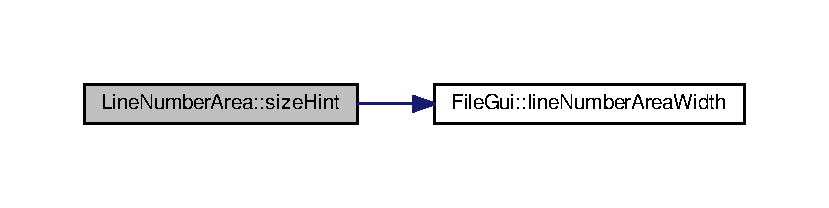
\includegraphics[width=350pt]{class_line_number_area_a5d31f7fb107bc1eefd7ae4974c095308_cgraph}
\end{center}
\end{figure}




\subsection{Member Data Documentation}
\hypertarget{class_line_number_area_a08ebbed0dba5e4740c0af7d006614922}{\index{Line\-Number\-Area@{Line\-Number\-Area}!file@{file}}
\index{file@{file}!LineNumberArea@{Line\-Number\-Area}}
\subsubsection[{file}]{\setlength{\rightskip}{0pt plus 5cm}{\bf File\-Gui}$\ast$ Line\-Number\-Area\-::file\hspace{0.3cm}{\ttfamily [private]}}}\label{class_line_number_area_a08ebbed0dba5e4740c0af7d006614922}


Definition at line 20 of file Line\-Number\-Area.\-h.



The documentation for this class was generated from the following files\-:\begin{DoxyCompactItemize}
\item 
/home/james/\-Net\-Beans\-Projects/ride/src/\hyperlink{_line_number_area_8h}{Line\-Number\-Area.\-h}\item 
/home/james/\-Net\-Beans\-Projects/ride/src/\hyperlink{_line_number_area_8cpp}{Line\-Number\-Area.\-cpp}\end{DoxyCompactItemize}

\hypertarget{class_master_actions}{\section{Master\-Actions Class Reference}
\label{class_master_actions}\index{Master\-Actions@{Master\-Actions}}
}


{\ttfamily \#include $<$Master\-Actions.\-h$>$}

Inheritance diagram for Master\-Actions\-:\begin{figure}[H]
\begin{center}
\leavevmode
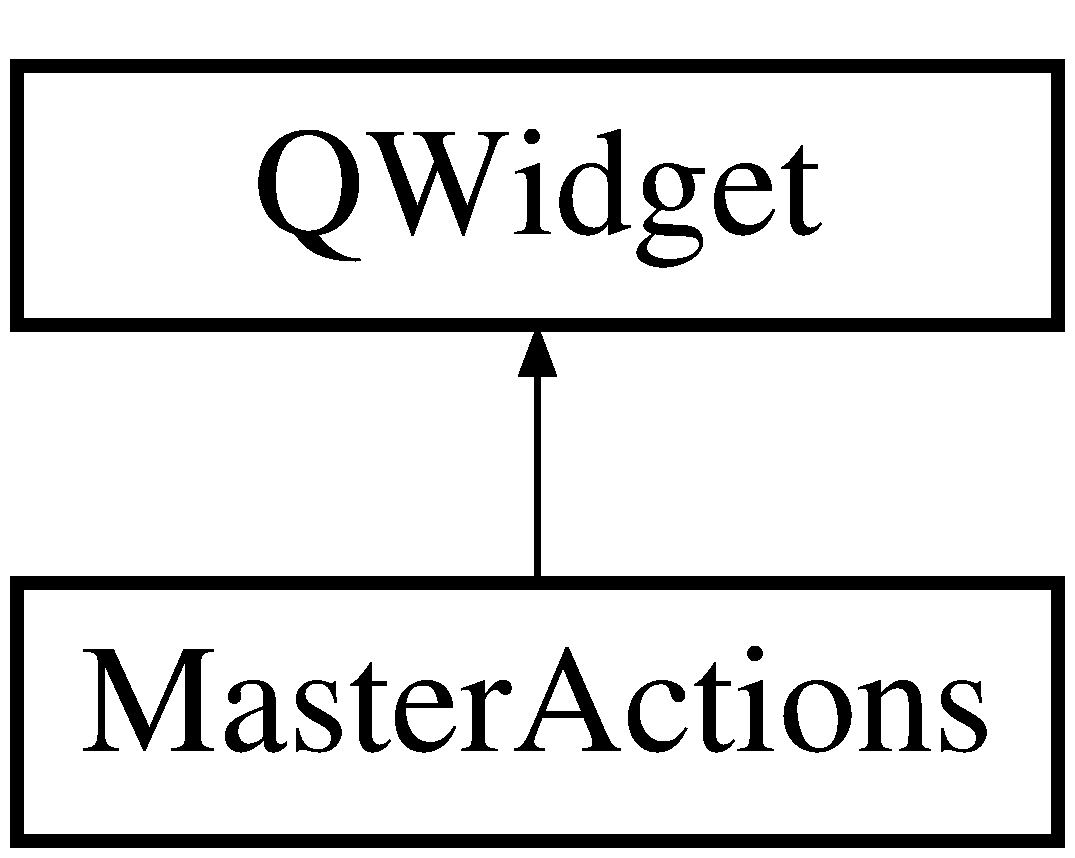
\includegraphics[height=2.000000cm]{class_master_actions}
\end{center}
\end{figure}
\subsection*{Public Member Functions}
\begin{DoxyCompactItemize}
\item 
\hyperlink{class_master_actions_ad8eb348b90e75f5876c30692930a2c22}{Master\-Actions} (Q\-Widget $\ast$parent=0)
\item 
void \hyperlink{class_master_actions_a9e2ff3903452d1212d530e20af9d7936}{init\-Actions} ()
\item 
void \hyperlink{class_master_actions_ab831fe700bf1327e6cde36f9272ecc11}{set\-North\-Tab\-Widget\-Ptr} (Q\-Tab\-Widget $\ast$\hyperlink{class_master_actions_a4fbb50c5700fd6b66ace4cff6d3bde3e}{north\-Tab\-Widget\-Ptr})
\item 
Q\-Tab\-Widget $\ast$ \hyperlink{class_master_actions_ac58b3c22042de182e6185e1700fa2f5e}{get\-North\-Tab\-Widget\-Ptr} ()
\item 
void \hyperlink{class_master_actions_a835def663e007647d721c2aa91d02f02}{set\-South\-Tab\-Widget\-Ptr} (\hyperlink{class_output_gui}{Output\-Gui} $\ast$\hyperlink{class_master_actions_a0cbcc4a5b82537a3f958c462bcaade46}{south\-Tab\-Widget\-Ptr})
\item 
\hyperlink{class_output_gui}{Output\-Gui} $\ast$ \hyperlink{class_master_actions_aafb5837208f5909593221be23ca3f22f}{get\-South\-Tab\-Widget\-Ptr} ()
\item 
void \hyperlink{class_master_actions_ae5856ce1f1a1d1f83622631512638dd8}{set\-Highlighter} (\hyperlink{class_highlighter}{Highlighter} $\ast$\hyperlink{class_master_actions_a50b1565db8b7780ec4e88e59953aa67b}{highlighter})
\item 
\hyperlink{class_highlighter}{Highlighter} $\ast$ \hyperlink{class_master_actions_a2b609608d4fdfe1f4abc4ba386e58923}{get\-Highlighter} ()
\item 
void \hyperlink{class_master_actions_a4fde279b855381679703cac9037deb08}{set\-New\-File\-Gui\-Ptr} (\hyperlink{class_new_file_gui}{New\-File\-Gui} $\ast$\hyperlink{class_master_actions_a8839c174acf071c0d9bfe450160218eb}{new\-File\-Gui\-Ptr})
\item 
\hyperlink{class_new_file_gui}{New\-File\-Gui} $\ast$ \hyperlink{class_master_actions_acb2a5079f7000c89fd0817db3ba46040}{get\-New\-File\-Gui\-Ptr} ()
\item 
void \hyperlink{class_master_actions_a4d26f5e2d62c71b71c4a198326b241f1}{set\-New\-Project\-Gui\-Ptr} (\hyperlink{class_new_project_gui}{New\-Project\-Gui} $\ast$\hyperlink{class_master_actions_a78733336a3d5fd3bbb55eaf0215f0d40}{new\-Project\-Gui\-Ptr})
\item 
\hyperlink{class_new_project_gui}{New\-Project\-Gui} $\ast$ \hyperlink{class_master_actions_a30b51649f46b8f105f8be5d9b4a6fb5f}{get\-New\-Project\-Gui\-Ptr} ()
\item 
void \hyperlink{class_master_actions_a78487f636588daf028a576b47703772e}{set\-Terminal\-Ptr} (\hyperlink{class_q_x_term}{Q\-X\-Term} $\ast$\hyperlink{class_master_actions_a540ec48ffb8bc7955f5630fac7b3865b}{terminal\-Ptr})
\item 
\hyperlink{class_q_x_term}{Q\-X\-Term} $\ast$ \hyperlink{class_master_actions_a1d6e583d7c6b63ca210ccc785e58c18d}{get\-Terminal\-Ptr} ()
\item 
void \hyperlink{class_master_actions_a67bf77b969dcbe752434110c8163d792}{set\-Run\-Gui\-Ptr} (\hyperlink{class_run_gui}{Run\-Gui} $\ast$\hyperlink{class_master_actions_ad7ff295f2e3067697e290afc4f0fd0df}{run\-Gui\-Ptr})
\item 
\hyperlink{class_run_gui}{Run\-Gui} $\ast$ \hyperlink{class_master_actions_a056278722ed1dbe98df15d1d073454bc}{get\-Run\-Gui\-Ptr} ()
\item 
void \hyperlink{class_master_actions_afc72dd08b2b6c8c25b8c4650b0446172}{set\-Open\-Project\-Gui\-Ptr} (\hyperlink{class_open_project_gui}{Open\-Project\-Gui} $\ast$\hyperlink{class_master_actions_a6caf7325dd9cb26f72c81a8c877db634}{open\-Project\-Gui\-Ptr})
\item 
\hyperlink{class_open_project_gui}{Open\-Project\-Gui} $\ast$ \hyperlink{class_master_actions_ab70b9336f1785ba7759b393d0b6a41db}{get\-Open\-Project\-Gui\-Ptr} ()
\item 
void \hyperlink{class_master_actions_a5e02bad0c35da48dcf7dc6a104d4a745}{set\-West\-Widget\-Ptr} (\hyperlink{class_file_tree_gui}{File\-Tree\-Gui} $\ast$\hyperlink{class_master_actions_a84f8a14213e1f05a00f1855b41a973de}{west\-Widget\-Ptr})
\item 
\hyperlink{class_file_tree_gui}{File\-Tree\-Gui} $\ast$ \hyperlink{class_master_actions_aae29be0bf5f9f2b8f1c7aac0c7efb288}{get\-West\-Widget\-Ptr} ()
\item 
void \hyperlink{class_master_actions_a983ce09c5c21c3cbf912472e878c7842}{set\-East\-Widget\-Ptr} (\hyperlink{class_navigator_gui}{Navigator\-Gui} $\ast$\hyperlink{class_master_actions_a24c61c608d67e766f996d3a430a7bae0}{east\-Widget\-Ptr})
\item 
\hyperlink{class_navigator_gui}{Navigator\-Gui} $\ast$ \hyperlink{class_master_actions_a863ab54858bacd76b50af788a6846e8e}{get\-East\-Widget\-Ptr} ()
\item 
void \hyperlink{class_master_actions_aad032f97113c45d9f02035b7e2ef605f}{set\-Build\-Ptr} (\hyperlink{class_build}{Build} $\ast$\hyperlink{class_master_actions_a204854f9bf284e221292497cdb7182ab}{build\-Ptr})
\item 
\hyperlink{class_build}{Build} $\ast$ \hyperlink{class_master_actions_aa1fb0f2857ad88742c874e22a308e4f4}{get\-Build\-Ptr} ()
\item 
void \hyperlink{class_master_actions_a4af05020cee8c5e80df586b03c20e765}{set\-New\-File\-Action\-Ptr} (Q\-Action $\ast$\hyperlink{class_master_actions_a4da658e527460b8d5b0a263820259e97}{new\-File\-Action\-Ptr})
\item 
Q\-Action $\ast$ \hyperlink{class_master_actions_a0ef76147044b06c8b951534a0d7ab7f2}{get\-New\-File\-Action\-Ptr} ()
\item 
void \hyperlink{class_master_actions_afe72189da4d2c5657f20d51fbcf6a62c}{set\-New\-Terminal\-Action\-Ptr} (Q\-Action $\ast$\hyperlink{class_master_actions_a6c3b1d9319fbf23f5a7cbe8305e16fc1}{new\-Terminal\-Action\-Ptr})
\item 
Q\-Action $\ast$ \hyperlink{class_master_actions_ae9f9f04302be1d7dc9fe902fc2597a1b}{get\-New\-Terminal\-Action\-Ptr} ()
\item 
void \hyperlink{class_master_actions_a4d6a5bfbd44ebe419d7cfa8295a54a39}{set\-New\-Project\-Action\-Ptr} (Q\-Action $\ast$\hyperlink{class_master_actions_a114ab55c27fc183af68ebaaa86748a82}{new\-Project\-Action\-Ptr})
\item 
Q\-Action $\ast$ \hyperlink{class_master_actions_a7065dfa244266181223b152795a996e9}{get\-New\-Project\-Action\-Ptr} ()
\item 
void \hyperlink{class_master_actions_abbbe38a813adedd51c5f7187c0d045a0}{set\-Open\-Project\-Action\-Ptr} (Q\-Action $\ast$\hyperlink{class_master_actions_a3b4d98cdbfaa8e287d420513a8df53ee}{open\-Project\-Action\-Ptr})
\item 
Q\-Action $\ast$ \hyperlink{class_master_actions_aac19d660169392d11b0ae1c2540cafb5}{get\-Open\-Project\-Action\-Ptr} ()
\item 
void \hyperlink{class_master_actions_a28b7a07a0c6932f5f8a55a778c1b2a0f}{set\-Save\-All\-Action\-Ptr} (Q\-Action $\ast$\hyperlink{class_master_actions_a4e9bf6410023b508d56f235903a44b5f}{save\-All\-Action\-Ptr})
\item 
Q\-Action $\ast$ \hyperlink{class_master_actions_afd7ef11ff065232fca47f971af02c5e5}{get\-Save\-All\-Action\-Ptr} ()
\item 
void \hyperlink{class_master_actions_ac1b4b1ac149aabb6530475503f715cd9}{set\-Undo\-Action\-Ptr} (Q\-Action $\ast$\hyperlink{class_master_actions_a23386959a2f60a89cc6ae1bff012c76c}{undo\-Action\-Ptr})
\item 
Q\-Action $\ast$ \hyperlink{class_master_actions_aeb84d87b232944fc289dd0425c79e1a7}{get\-Undo\-Action\-Ptr} ()
\item 
void \hyperlink{class_master_actions_aa470d0d50071545456339dd6efd1cd29}{set\-Redo\-Action\-Ptr} (Q\-Action $\ast$\hyperlink{class_master_actions_a7936a9bf0e7418cd864b2fb1ab786d09}{redo\-Action\-Ptr})
\item 
Q\-Action $\ast$ \hyperlink{class_master_actions_ab2015974980e97a75d5d91037be9545b}{get\-Redo\-Action\-Ptr} ()
\item 
void \hyperlink{class_master_actions_a3ec5d73b64fdadc42fe7eb63a3792d53}{set\-Set\-Project\-Config\-Action\-Ptr} (Q\-Action $\ast$\hyperlink{class_master_actions_abe52f232f77f5a5bff35c8e3dadb3d80}{set\-Project\-Config\-Action\-Ptr})
\item 
Q\-Action $\ast$ \hyperlink{class_master_actions_ad81b766a2f083ba53c529cd3f3582cd0}{get\-Set\-Project\-Config\-Action\-Ptr} ()
\item 
void \hyperlink{class_master_actions_a575820c5279053703a99071151ff82c4}{set\-Build\-Action\-Ptr} (Q\-Action $\ast$set\-Build\-Action\-Ptr)
\item 
Q\-Action $\ast$ \hyperlink{class_master_actions_a2c89cb4aa70c13526d98e449a1e3a1b9}{get\-Build\-Action\-Ptr} ()
\item 
void \hyperlink{class_master_actions_a9ed58e080af95465715e9be1c9ee71c6}{set\-Clean\-And\-Build\-Action\-Ptr} (Q\-Action $\ast$\hyperlink{class_master_actions_a2c0f332975bec2424d4af212ab566c5a}{clean\-And\-Build\-Action\-Ptr})
\item 
Q\-Action $\ast$ \hyperlink{class_master_actions_af23ec377bb3603963735d30876e6147e}{get\-Clean\-And\-Build\-Action\-Ptr} ()
\item 
void \hyperlink{class_master_actions_a8b4ef0d552c3dac5c81cf65502650ae5}{set\-Config\-For\-Run\-Action\-Ptr} (Q\-Action $\ast$\hyperlink{class_master_actions_acd6548d1110ae426f384bfeb6acc9c1f}{config\-For\-Run\-Action\-Ptr})
\item 
Q\-Action $\ast$ \hyperlink{class_master_actions_a5266af068fe6ec921cca9e84b9ad7c13}{get\-Config\-For\-Run\-Action\-Ptr} ()
\item 
void \hyperlink{class_master_actions_a28ac730c1a6dd78adf10e1ffcda14aaa}{set\-Run\-Action\-Ptr} (Q\-Action $\ast$\hyperlink{class_master_actions_a3377fe0ddc45ce50119766c8a903c039}{run\-Action\-Ptr})
\item 
Q\-Action $\ast$ \hyperlink{class_master_actions_a99017fd6ad87557fb0dbbf60ced23a23}{get\-Run\-Action\-Ptr} ()
\item 
void \hyperlink{class_master_actions_a66be4fac5aa53c8c40128e1cfab35676}{set\-Debug\-Action\-Ptr} (Q\-Action $\ast$\hyperlink{class_master_actions_ae37993bbbed4a238ea3b11089ac46a61}{debug\-Action\-Ptr})
\item 
Q\-Action $\ast$ \hyperlink{class_master_actions_a38c19285a782f80fd538243f1a7119bc}{get\-Debug\-Action\-Ptr} ()
\item 
void \hyperlink{class_master_actions_a785e8465b91e563926ab0ef021907128}{set\-Git\-Action\-Ptr} (Q\-Action $\ast$profile\-Proj\-Action\-Ptr)
\item 
Q\-Action $\ast$ \hyperlink{class_master_actions_a512f6344322707bd745ac413036238df}{get\-Git\-Action\-Ptr} ()
\item 
void \hyperlink{class_master_actions_ac476afca80285f13a11ef0e5cd10778c}{set\-Output\-South\-Action\-Ptr} (Q\-Action $\ast$\hyperlink{class_master_actions_a5b7a85c6728274eb0fcb48924044b9f6}{output\-South\-Action\-Ptr})
\item 
Q\-Action $\ast$ \hyperlink{class_master_actions_acb9a1d3eb98cab06fd2ae5b9faf30fc3}{get\-Output\-South\-Action\-Ptr} ()
\item 
void \hyperlink{class_master_actions_a718fd78374dab2c701fef75aa9e7a2fe}{set\-Terminal\-South\-Action\-Ptr} (Q\-Action $\ast$\hyperlink{class_master_actions_ad96c9f17230e162e9a9f39a867101a53}{terminal\-South\-Action\-Ptr})
\item 
Q\-Action $\ast$ \hyperlink{class_master_actions_ae9a9fe05579b18051c29f7e54d50a06b}{get\-Terminal\-South\-Action\-Ptr} ()
\item 
void \hyperlink{class_master_actions_a42342f8666f61fd111f2cba1fd082d49}{set\-Nav\-East\-Action\-Ptr} (Q\-Action $\ast$nav\-East\-Actionptr)
\item 
Q\-Action $\ast$ \hyperlink{class_master_actions_af74c6ae5449f5f738eff1575defbde16}{get\-Nav\-East\-Action\-Ptr} ()
\item 
void \hyperlink{class_master_actions_ad0522fc89be3dd4451d84300208b5925}{set\-Project\-West\-Action\-Ptr} (Q\-Action $\ast$\hyperlink{class_master_actions_aa4160469d2e9a840448c49e95bcfa9e5}{project\-West\-Action\-Ptr})
\item 
Q\-Action $\ast$ \hyperlink{class_master_actions_a97e9c1a3bd46f70d1afd640ac06cc18d}{get\-Project\-West\-Action\-Ptr} ()
\item 
{\footnotesize template$<$class X $>$ }\\void \hyperlink{class_master_actions_a24f67a69e013feac51a24a34d32f2c40}{connect\-To\-New\-File\-Action} (X $\ast$component)
\item 
{\footnotesize template$<$class X $>$ }\\void \hyperlink{class_master_actions_aeca9ddb448704bcc3a7e9ac3a66d5b57}{connect\-To\-New\-Terminal\-Action} (X $\ast$component)
\item 
{\footnotesize template$<$class X $>$ }\\void \hyperlink{class_master_actions_a7eb69b0a616b949086f7422394f6c881}{connect\-To\-New\-Project\-Action} (X $\ast$component)
\item 
{\footnotesize template$<$class X $>$ }\\void \hyperlink{class_master_actions_aa792c3936e0b0b4c016d01ad4a1c5803}{connect\-To\-Open\-Project\-Action} (X $\ast$component)
\item 
{\footnotesize template$<$class X $>$ }\\void \hyperlink{class_master_actions_ab859d0b5419ae5f17504e8fdd83be4be}{connect\-To\-Save\-All\-Action} (X $\ast$component)
\item 
{\footnotesize template$<$class X $>$ }\\void \hyperlink{class_master_actions_a6590f8772608e4d99efbf16ef9625b78}{connect\-To\-Undo\-Action} (X $\ast$component)
\item 
{\footnotesize template$<$class X $>$ }\\void \hyperlink{class_master_actions_a6077c09ff4426c4a99eaa33ff12f22e4}{connect\-To\-Redo\-Action} (X $\ast$component)
\item 
{\footnotesize template$<$class X $>$ }\\void \hyperlink{class_master_actions_a5e25d464651d37d48c7e6a4714130dd7}{connect\-To\-Set\-Project\-Config\-Action} (X $\ast$component)
\item 
{\footnotesize template$<$class X $>$ }\\void \hyperlink{class_master_actions_a9625507b1a412bd95bdc13ae54bc68a2}{connect\-To\-Build\-Action} (X $\ast$component)
\item 
{\footnotesize template$<$class X $>$ }\\void \hyperlink{class_master_actions_a86232c67d3599a28c6b5238eb6dd4e88}{connect\-To\-Clean\-And\-Build\-Action} (X $\ast$component)
\item 
{\footnotesize template$<$class X $>$ }\\void \hyperlink{class_master_actions_a87ff14d6fdf08f3730bb733747335dcb}{connect\-To\-Config\-For\-Run\-Action} (X $\ast$component)
\item 
{\footnotesize template$<$class X $>$ }\\void \hyperlink{class_master_actions_a73ec685aa0f239226bdda78857b9e234}{connect\-To\-Run\-Action} (X $\ast$component)
\item 
{\footnotesize template$<$class X $>$ }\\void \hyperlink{class_master_actions_a9c1baa889fbb545dc9607044839d5813}{connect\-To\-Debug\-Action} (X $\ast$component)
\item 
{\footnotesize template$<$class X $>$ }\\void \hyperlink{class_master_actions_a6624b38f9a52128e261d78f0313fa99d}{connect\-To\-Git\-Action} (X $\ast$component)
\item 
{\footnotesize template$<$class X $>$ }\\void \hyperlink{class_master_actions_a0ccac38f3166e1410f09f20e27b0d020}{connect\-To\-Output\-South\-Action} (X $\ast$component)
\item 
{\footnotesize template$<$class X $>$ }\\void \hyperlink{class_master_actions_a9f7d8a2bd25c903cbb62be5e9a9ce8fc}{connect\-To\-Terminal\-South\-Action} (X $\ast$component)
\item 
{\footnotesize template$<$class X $>$ }\\void \hyperlink{class_master_actions_ab8028a378675e16f2d9ae4a42a7114be}{connect\-To\-Nav\-East\-Action} (X $\ast$component)
\item 
{\footnotesize template$<$class X $>$ }\\void \hyperlink{class_master_actions_ad8311d5ad31b045095be98a9e29db1bf}{connect\-To\-Project\-West\-Action} (X $\ast$component)
\item 
Q\-String $\ast$ \hyperlink{class_master_actions_ad215eb9ceed2d0cd3552585f3dfa3b62}{to\-String} ()
\item 
\hyperlink{class_master_actions_a2504de3ca736a30530296fc9b44fb55b}{$\sim$\-Master\-Actions} ()
\end{DoxyCompactItemize}
\subsection*{Private Slots}
\begin{DoxyCompactItemize}
\item 
void \hyperlink{class_master_actions_a75943822eee1dbbc3e7c6c1dda4780a0}{handle\-New\-File\-Action\-Slot} ()
\item 
void \hyperlink{class_master_actions_af1fa0d0d7b074abb49ae5dd6bccffbe9}{handle\-New\-Terminal\-Action\-Slot} ()
\item 
void \hyperlink{class_master_actions_a81d07306e15f16a66e992138faccfab5}{handle\-New\-Project\-Action\-Slot} ()
\item 
void \hyperlink{class_master_actions_abefe5adf2e269a408626ea1caee182ca}{handle\-Open\-Project\-Action\-Slot} ()
\item 
void \hyperlink{class_master_actions_a92d9fcaac21c09534c568b3aca195a87}{handle\-Save\-All\-Action\-Slot} ()
\item 
void \hyperlink{class_master_actions_a87a24d9944e6140a6ae0de92dc8e5647}{handle\-Undo\-Action\-Slot} ()
\item 
void \hyperlink{class_master_actions_a7aa83031542aeafb3f3afe244ce2cd67}{handle\-Redo\-Action\-Slot} ()
\item 
void \hyperlink{class_master_actions_a8b46b8a5873dfff5a85e21a7e636b4bf}{handle\-Set\-Project\-Config\-Action\-Slot} ()
\item 
void \hyperlink{class_master_actions_aa9af30e92d9f9e4ffb8044f092b06d07}{handle\-Build\-Action\-Slot} ()
\item 
void \hyperlink{class_master_actions_ac3621bfbde9a2b681d4d35ae72bd6f14}{handle\-Clean\-And\-Build\-Action\-Slot} ()
\item 
void \hyperlink{class_master_actions_a294fc01ac639ffcdf9b76378f0d21306}{handle\-Config\-For\-Run\-Action\-Slot} ()
\item 
void \hyperlink{class_master_actions_a8504741522d18cb1a5fb21b6ad6de14b}{handle\-Run\-Action\-Slot} ()
\item 
void \hyperlink{class_master_actions_acc96d5f9401e97aa2a4700a47cfa71bd}{handle\-Debug\-Action\-Slot} ()
\item 
void \hyperlink{class_master_actions_ac8b0e41e5f68cdc5c845ec9184b2cd6d}{handle\-Git\-Action\-Slot} ()
\item 
void \hyperlink{class_master_actions_afb11d896980c526784b05a440e6f21ac}{handle\-Output\-South\-Action\-Slot} ()
\item 
void \hyperlink{class_master_actions_a3f3ec7277966d98a9fc5df5ceca1fa97}{handle\-Terminal\-South\-Action\-Slot} ()
\item 
void \hyperlink{class_master_actions_a86d0a64d13866d196c05906dfae37b73}{handle\-Nav\-East\-Action\-Slot} ()
\item 
void \hyperlink{class_master_actions_a64bf020d68866c8941c01929879eb839}{handle\-Project\-West\-Action\-Slot} ()
\end{DoxyCompactItemize}
\subsection*{Private Attributes}
\begin{DoxyCompactItemize}
\item 
Q\-Action $\ast$ \hyperlink{class_master_actions_a4da658e527460b8d5b0a263820259e97}{new\-File\-Action\-Ptr}
\item 
Q\-Action $\ast$ \hyperlink{class_master_actions_a6c3b1d9319fbf23f5a7cbe8305e16fc1}{new\-Terminal\-Action\-Ptr}
\item 
Q\-Action $\ast$ \hyperlink{class_master_actions_a114ab55c27fc183af68ebaaa86748a82}{new\-Project\-Action\-Ptr}
\item 
Q\-Action $\ast$ \hyperlink{class_master_actions_a3b4d98cdbfaa8e287d420513a8df53ee}{open\-Project\-Action\-Ptr}
\item 
Q\-Action $\ast$ \hyperlink{class_master_actions_a4e9bf6410023b508d56f235903a44b5f}{save\-All\-Action\-Ptr}
\item 
Q\-Action $\ast$ \hyperlink{class_master_actions_a23386959a2f60a89cc6ae1bff012c76c}{undo\-Action\-Ptr}
\item 
Q\-Action $\ast$ \hyperlink{class_master_actions_a7936a9bf0e7418cd864b2fb1ab786d09}{redo\-Action\-Ptr}
\item 
Q\-Action $\ast$ \hyperlink{class_master_actions_abe52f232f77f5a5bff35c8e3dadb3d80}{set\-Project\-Config\-Action\-Ptr}
\item 
Q\-Action $\ast$ \hyperlink{class_master_actions_a627d91b89d122dd27addc931d1c91ca0}{build\-Action\-Ptr}
\item 
Q\-Action $\ast$ \hyperlink{class_master_actions_a2c0f332975bec2424d4af212ab566c5a}{clean\-And\-Build\-Action\-Ptr}
\item 
Q\-Action $\ast$ \hyperlink{class_master_actions_acd6548d1110ae426f384bfeb6acc9c1f}{config\-For\-Run\-Action\-Ptr}
\item 
Q\-Action $\ast$ \hyperlink{class_master_actions_a3377fe0ddc45ce50119766c8a903c039}{run\-Action\-Ptr}
\item 
Q\-Action $\ast$ \hyperlink{class_master_actions_ae37993bbbed4a238ea3b11089ac46a61}{debug\-Action\-Ptr}
\item 
Q\-Action $\ast$ \hyperlink{class_master_actions_ac9e25741cf358793122b687e82f7bb85}{git\-Action\-Ptr}
\item 
Q\-Action $\ast$ \hyperlink{class_master_actions_a5b7a85c6728274eb0fcb48924044b9f6}{output\-South\-Action\-Ptr}
\item 
Q\-Action $\ast$ \hyperlink{class_master_actions_ad96c9f17230e162e9a9f39a867101a53}{terminal\-South\-Action\-Ptr}
\item 
Q\-Action $\ast$ \hyperlink{class_master_actions_aa084a718ec328fbb6645bdb23c995df1}{nav\-East\-Action\-Ptr}
\item 
Q\-Action $\ast$ \hyperlink{class_master_actions_aa4160469d2e9a840448c49e95bcfa9e5}{project\-West\-Action\-Ptr}
\item 
Q\-Tab\-Widget $\ast$ \hyperlink{class_master_actions_a4fbb50c5700fd6b66ace4cff6d3bde3e}{north\-Tab\-Widget\-Ptr}
\item 
\hyperlink{class_output_gui}{Output\-Gui} $\ast$ \hyperlink{class_master_actions_a0cbcc4a5b82537a3f958c462bcaade46}{south\-Tab\-Widget\-Ptr}
\item 
\hyperlink{class_highlighter}{Highlighter} $\ast$ \hyperlink{class_master_actions_a50b1565db8b7780ec4e88e59953aa67b}{highlighter}
\item 
\hyperlink{class_new_file_gui}{New\-File\-Gui} $\ast$ \hyperlink{class_master_actions_a8839c174acf071c0d9bfe450160218eb}{new\-File\-Gui\-Ptr}
\item 
\hyperlink{class_new_project_gui}{New\-Project\-Gui} $\ast$ \hyperlink{class_master_actions_a78733336a3d5fd3bbb55eaf0215f0d40}{new\-Project\-Gui\-Ptr}
\item 
\hyperlink{class_q_x_term}{Q\-X\-Term} $\ast$ \hyperlink{class_master_actions_a540ec48ffb8bc7955f5630fac7b3865b}{terminal\-Ptr}
\item 
\hyperlink{class_run_gui}{Run\-Gui} $\ast$ \hyperlink{class_master_actions_ad7ff295f2e3067697e290afc4f0fd0df}{run\-Gui\-Ptr}
\item 
\hyperlink{class_open_project_gui}{Open\-Project\-Gui} $\ast$ \hyperlink{class_master_actions_a6caf7325dd9cb26f72c81a8c877db634}{open\-Project\-Gui\-Ptr}
\item 
\hyperlink{class_file_tree_gui}{File\-Tree\-Gui} $\ast$ \hyperlink{class_master_actions_a84f8a14213e1f05a00f1855b41a973de}{west\-Widget\-Ptr}
\item 
\hyperlink{class_navigator_gui}{Navigator\-Gui} $\ast$ \hyperlink{class_master_actions_a24c61c608d67e766f996d3a430a7bae0}{east\-Widget\-Ptr}
\item 
\hyperlink{class_build}{Build} $\ast$ \hyperlink{class_master_actions_a204854f9bf284e221292497cdb7182ab}{build\-Ptr}
\end{DoxyCompactItemize}


\subsection{Constructor \& Destructor Documentation}
\hypertarget{class_master_actions_ad8eb348b90e75f5876c30692930a2c22}{\index{Master\-Actions@{Master\-Actions}!Master\-Actions@{Master\-Actions}}
\index{Master\-Actions@{Master\-Actions}!MasterActions@{Master\-Actions}}
\subsubsection[{Master\-Actions}]{\setlength{\rightskip}{0pt plus 5cm}Master\-Actions\-::\-Master\-Actions (
\begin{DoxyParamCaption}
\item[{Q\-Widget $\ast$}]{parent = {\ttfamily 0}}
\end{DoxyParamCaption}
)}}\label{class_master_actions_ad8eb348b90e75f5876c30692930a2c22}
\hypertarget{class_master_actions_a2504de3ca736a30530296fc9b44fb55b}{\index{Master\-Actions@{Master\-Actions}!$\sim$\-Master\-Actions@{$\sim$\-Master\-Actions}}
\index{$\sim$\-Master\-Actions@{$\sim$\-Master\-Actions}!MasterActions@{Master\-Actions}}
\subsubsection[{$\sim$\-Master\-Actions}]{\setlength{\rightskip}{0pt plus 5cm}Master\-Actions\-::$\sim$\-Master\-Actions (
\begin{DoxyParamCaption}
{}
\end{DoxyParamCaption}
)}}\label{class_master_actions_a2504de3ca736a30530296fc9b44fb55b}


\subsection{Member Function Documentation}
\hypertarget{class_master_actions_a9625507b1a412bd95bdc13ae54bc68a2}{\index{Master\-Actions@{Master\-Actions}!connect\-To\-Build\-Action@{connect\-To\-Build\-Action}}
\index{connect\-To\-Build\-Action@{connect\-To\-Build\-Action}!MasterActions@{Master\-Actions}}
\subsubsection[{connect\-To\-Build\-Action}]{\setlength{\rightskip}{0pt plus 5cm}template$<$class X $>$ void Master\-Actions\-::connect\-To\-Build\-Action (
\begin{DoxyParamCaption}
\item[{X $\ast$}]{component}
\end{DoxyParamCaption}
)}}\label{class_master_actions_a9625507b1a412bd95bdc13ae54bc68a2}
\hypertarget{class_master_actions_a86232c67d3599a28c6b5238eb6dd4e88}{\index{Master\-Actions@{Master\-Actions}!connect\-To\-Clean\-And\-Build\-Action@{connect\-To\-Clean\-And\-Build\-Action}}
\index{connect\-To\-Clean\-And\-Build\-Action@{connect\-To\-Clean\-And\-Build\-Action}!MasterActions@{Master\-Actions}}
\subsubsection[{connect\-To\-Clean\-And\-Build\-Action}]{\setlength{\rightskip}{0pt plus 5cm}template$<$class X $>$ void Master\-Actions\-::connect\-To\-Clean\-And\-Build\-Action (
\begin{DoxyParamCaption}
\item[{X $\ast$}]{component}
\end{DoxyParamCaption}
)}}\label{class_master_actions_a86232c67d3599a28c6b5238eb6dd4e88}
\hypertarget{class_master_actions_a87ff14d6fdf08f3730bb733747335dcb}{\index{Master\-Actions@{Master\-Actions}!connect\-To\-Config\-For\-Run\-Action@{connect\-To\-Config\-For\-Run\-Action}}
\index{connect\-To\-Config\-For\-Run\-Action@{connect\-To\-Config\-For\-Run\-Action}!MasterActions@{Master\-Actions}}
\subsubsection[{connect\-To\-Config\-For\-Run\-Action}]{\setlength{\rightskip}{0pt plus 5cm}template$<$class X $>$ void Master\-Actions\-::connect\-To\-Config\-For\-Run\-Action (
\begin{DoxyParamCaption}
\item[{X $\ast$}]{component}
\end{DoxyParamCaption}
)}}\label{class_master_actions_a87ff14d6fdf08f3730bb733747335dcb}
\hypertarget{class_master_actions_a9c1baa889fbb545dc9607044839d5813}{\index{Master\-Actions@{Master\-Actions}!connect\-To\-Debug\-Action@{connect\-To\-Debug\-Action}}
\index{connect\-To\-Debug\-Action@{connect\-To\-Debug\-Action}!MasterActions@{Master\-Actions}}
\subsubsection[{connect\-To\-Debug\-Action}]{\setlength{\rightskip}{0pt plus 5cm}template$<$class X $>$ void Master\-Actions\-::connect\-To\-Debug\-Action (
\begin{DoxyParamCaption}
\item[{X $\ast$}]{component}
\end{DoxyParamCaption}
)}}\label{class_master_actions_a9c1baa889fbb545dc9607044839d5813}
\hypertarget{class_master_actions_a6624b38f9a52128e261d78f0313fa99d}{\index{Master\-Actions@{Master\-Actions}!connect\-To\-Git\-Action@{connect\-To\-Git\-Action}}
\index{connect\-To\-Git\-Action@{connect\-To\-Git\-Action}!MasterActions@{Master\-Actions}}
\subsubsection[{connect\-To\-Git\-Action}]{\setlength{\rightskip}{0pt plus 5cm}template$<$class X $>$ void Master\-Actions\-::connect\-To\-Git\-Action (
\begin{DoxyParamCaption}
\item[{X $\ast$}]{component}
\end{DoxyParamCaption}
)}}\label{class_master_actions_a6624b38f9a52128e261d78f0313fa99d}
\hypertarget{class_master_actions_ab8028a378675e16f2d9ae4a42a7114be}{\index{Master\-Actions@{Master\-Actions}!connect\-To\-Nav\-East\-Action@{connect\-To\-Nav\-East\-Action}}
\index{connect\-To\-Nav\-East\-Action@{connect\-To\-Nav\-East\-Action}!MasterActions@{Master\-Actions}}
\subsubsection[{connect\-To\-Nav\-East\-Action}]{\setlength{\rightskip}{0pt plus 5cm}template$<$class X $>$ void Master\-Actions\-::connect\-To\-Nav\-East\-Action (
\begin{DoxyParamCaption}
\item[{X $\ast$}]{component}
\end{DoxyParamCaption}
)}}\label{class_master_actions_ab8028a378675e16f2d9ae4a42a7114be}
\hypertarget{class_master_actions_a24f67a69e013feac51a24a34d32f2c40}{\index{Master\-Actions@{Master\-Actions}!connect\-To\-New\-File\-Action@{connect\-To\-New\-File\-Action}}
\index{connect\-To\-New\-File\-Action@{connect\-To\-New\-File\-Action}!MasterActions@{Master\-Actions}}
\subsubsection[{connect\-To\-New\-File\-Action}]{\setlength{\rightskip}{0pt plus 5cm}template$<$class X $>$ void Master\-Actions\-::connect\-To\-New\-File\-Action (
\begin{DoxyParamCaption}
\item[{X $\ast$}]{component}
\end{DoxyParamCaption}
)}}\label{class_master_actions_a24f67a69e013feac51a24a34d32f2c40}
\hypertarget{class_master_actions_a7eb69b0a616b949086f7422394f6c881}{\index{Master\-Actions@{Master\-Actions}!connect\-To\-New\-Project\-Action@{connect\-To\-New\-Project\-Action}}
\index{connect\-To\-New\-Project\-Action@{connect\-To\-New\-Project\-Action}!MasterActions@{Master\-Actions}}
\subsubsection[{connect\-To\-New\-Project\-Action}]{\setlength{\rightskip}{0pt plus 5cm}template$<$class X $>$ void Master\-Actions\-::connect\-To\-New\-Project\-Action (
\begin{DoxyParamCaption}
\item[{X $\ast$}]{component}
\end{DoxyParamCaption}
)}}\label{class_master_actions_a7eb69b0a616b949086f7422394f6c881}
\hypertarget{class_master_actions_aeca9ddb448704bcc3a7e9ac3a66d5b57}{\index{Master\-Actions@{Master\-Actions}!connect\-To\-New\-Terminal\-Action@{connect\-To\-New\-Terminal\-Action}}
\index{connect\-To\-New\-Terminal\-Action@{connect\-To\-New\-Terminal\-Action}!MasterActions@{Master\-Actions}}
\subsubsection[{connect\-To\-New\-Terminal\-Action}]{\setlength{\rightskip}{0pt plus 5cm}template$<$class X $>$ void Master\-Actions\-::connect\-To\-New\-Terminal\-Action (
\begin{DoxyParamCaption}
\item[{X $\ast$}]{component}
\end{DoxyParamCaption}
)}}\label{class_master_actions_aeca9ddb448704bcc3a7e9ac3a66d5b57}
\hypertarget{class_master_actions_aa792c3936e0b0b4c016d01ad4a1c5803}{\index{Master\-Actions@{Master\-Actions}!connect\-To\-Open\-Project\-Action@{connect\-To\-Open\-Project\-Action}}
\index{connect\-To\-Open\-Project\-Action@{connect\-To\-Open\-Project\-Action}!MasterActions@{Master\-Actions}}
\subsubsection[{connect\-To\-Open\-Project\-Action}]{\setlength{\rightskip}{0pt plus 5cm}template$<$class X $>$ void Master\-Actions\-::connect\-To\-Open\-Project\-Action (
\begin{DoxyParamCaption}
\item[{X $\ast$}]{component}
\end{DoxyParamCaption}
)}}\label{class_master_actions_aa792c3936e0b0b4c016d01ad4a1c5803}
\hypertarget{class_master_actions_a0ccac38f3166e1410f09f20e27b0d020}{\index{Master\-Actions@{Master\-Actions}!connect\-To\-Output\-South\-Action@{connect\-To\-Output\-South\-Action}}
\index{connect\-To\-Output\-South\-Action@{connect\-To\-Output\-South\-Action}!MasterActions@{Master\-Actions}}
\subsubsection[{connect\-To\-Output\-South\-Action}]{\setlength{\rightskip}{0pt plus 5cm}template$<$class X $>$ void Master\-Actions\-::connect\-To\-Output\-South\-Action (
\begin{DoxyParamCaption}
\item[{X $\ast$}]{component}
\end{DoxyParamCaption}
)}}\label{class_master_actions_a0ccac38f3166e1410f09f20e27b0d020}
\hypertarget{class_master_actions_ad8311d5ad31b045095be98a9e29db1bf}{\index{Master\-Actions@{Master\-Actions}!connect\-To\-Project\-West\-Action@{connect\-To\-Project\-West\-Action}}
\index{connect\-To\-Project\-West\-Action@{connect\-To\-Project\-West\-Action}!MasterActions@{Master\-Actions}}
\subsubsection[{connect\-To\-Project\-West\-Action}]{\setlength{\rightskip}{0pt plus 5cm}template$<$class X $>$ void Master\-Actions\-::connect\-To\-Project\-West\-Action (
\begin{DoxyParamCaption}
\item[{X $\ast$}]{component}
\end{DoxyParamCaption}
)}}\label{class_master_actions_ad8311d5ad31b045095be98a9e29db1bf}
\hypertarget{class_master_actions_a6077c09ff4426c4a99eaa33ff12f22e4}{\index{Master\-Actions@{Master\-Actions}!connect\-To\-Redo\-Action@{connect\-To\-Redo\-Action}}
\index{connect\-To\-Redo\-Action@{connect\-To\-Redo\-Action}!MasterActions@{Master\-Actions}}
\subsubsection[{connect\-To\-Redo\-Action}]{\setlength{\rightskip}{0pt plus 5cm}template$<$class X $>$ void Master\-Actions\-::connect\-To\-Redo\-Action (
\begin{DoxyParamCaption}
\item[{X $\ast$}]{component}
\end{DoxyParamCaption}
)}}\label{class_master_actions_a6077c09ff4426c4a99eaa33ff12f22e4}
\hypertarget{class_master_actions_a73ec685aa0f239226bdda78857b9e234}{\index{Master\-Actions@{Master\-Actions}!connect\-To\-Run\-Action@{connect\-To\-Run\-Action}}
\index{connect\-To\-Run\-Action@{connect\-To\-Run\-Action}!MasterActions@{Master\-Actions}}
\subsubsection[{connect\-To\-Run\-Action}]{\setlength{\rightskip}{0pt plus 5cm}template$<$class X $>$ void Master\-Actions\-::connect\-To\-Run\-Action (
\begin{DoxyParamCaption}
\item[{X $\ast$}]{component}
\end{DoxyParamCaption}
)}}\label{class_master_actions_a73ec685aa0f239226bdda78857b9e234}
\hypertarget{class_master_actions_ab859d0b5419ae5f17504e8fdd83be4be}{\index{Master\-Actions@{Master\-Actions}!connect\-To\-Save\-All\-Action@{connect\-To\-Save\-All\-Action}}
\index{connect\-To\-Save\-All\-Action@{connect\-To\-Save\-All\-Action}!MasterActions@{Master\-Actions}}
\subsubsection[{connect\-To\-Save\-All\-Action}]{\setlength{\rightskip}{0pt plus 5cm}template$<$class X $>$ void Master\-Actions\-::connect\-To\-Save\-All\-Action (
\begin{DoxyParamCaption}
\item[{X $\ast$}]{component}
\end{DoxyParamCaption}
)}}\label{class_master_actions_ab859d0b5419ae5f17504e8fdd83be4be}
\hypertarget{class_master_actions_a5e25d464651d37d48c7e6a4714130dd7}{\index{Master\-Actions@{Master\-Actions}!connect\-To\-Set\-Project\-Config\-Action@{connect\-To\-Set\-Project\-Config\-Action}}
\index{connect\-To\-Set\-Project\-Config\-Action@{connect\-To\-Set\-Project\-Config\-Action}!MasterActions@{Master\-Actions}}
\subsubsection[{connect\-To\-Set\-Project\-Config\-Action}]{\setlength{\rightskip}{0pt plus 5cm}template$<$class X $>$ void Master\-Actions\-::connect\-To\-Set\-Project\-Config\-Action (
\begin{DoxyParamCaption}
\item[{X $\ast$}]{component}
\end{DoxyParamCaption}
)}}\label{class_master_actions_a5e25d464651d37d48c7e6a4714130dd7}
\hypertarget{class_master_actions_a9f7d8a2bd25c903cbb62be5e9a9ce8fc}{\index{Master\-Actions@{Master\-Actions}!connect\-To\-Terminal\-South\-Action@{connect\-To\-Terminal\-South\-Action}}
\index{connect\-To\-Terminal\-South\-Action@{connect\-To\-Terminal\-South\-Action}!MasterActions@{Master\-Actions}}
\subsubsection[{connect\-To\-Terminal\-South\-Action}]{\setlength{\rightskip}{0pt plus 5cm}template$<$class X $>$ void Master\-Actions\-::connect\-To\-Terminal\-South\-Action (
\begin{DoxyParamCaption}
\item[{X $\ast$}]{component}
\end{DoxyParamCaption}
)}}\label{class_master_actions_a9f7d8a2bd25c903cbb62be5e9a9ce8fc}
\hypertarget{class_master_actions_a6590f8772608e4d99efbf16ef9625b78}{\index{Master\-Actions@{Master\-Actions}!connect\-To\-Undo\-Action@{connect\-To\-Undo\-Action}}
\index{connect\-To\-Undo\-Action@{connect\-To\-Undo\-Action}!MasterActions@{Master\-Actions}}
\subsubsection[{connect\-To\-Undo\-Action}]{\setlength{\rightskip}{0pt plus 5cm}template$<$class X $>$ void Master\-Actions\-::connect\-To\-Undo\-Action (
\begin{DoxyParamCaption}
\item[{X $\ast$}]{component}
\end{DoxyParamCaption}
)}}\label{class_master_actions_a6590f8772608e4d99efbf16ef9625b78}
\hypertarget{class_master_actions_a2c89cb4aa70c13526d98e449a1e3a1b9}{\index{Master\-Actions@{Master\-Actions}!get\-Build\-Action\-Ptr@{get\-Build\-Action\-Ptr}}
\index{get\-Build\-Action\-Ptr@{get\-Build\-Action\-Ptr}!MasterActions@{Master\-Actions}}
\subsubsection[{get\-Build\-Action\-Ptr}]{\setlength{\rightskip}{0pt plus 5cm}Q\-Action $\ast$ Master\-Actions\-::get\-Build\-Action\-Ptr (
\begin{DoxyParamCaption}
{}
\end{DoxyParamCaption}
)}}\label{class_master_actions_a2c89cb4aa70c13526d98e449a1e3a1b9}
\hypertarget{class_master_actions_aa1fb0f2857ad88742c874e22a308e4f4}{\index{Master\-Actions@{Master\-Actions}!get\-Build\-Ptr@{get\-Build\-Ptr}}
\index{get\-Build\-Ptr@{get\-Build\-Ptr}!MasterActions@{Master\-Actions}}
\subsubsection[{get\-Build\-Ptr}]{\setlength{\rightskip}{0pt plus 5cm}{\bf Build} $\ast$ Master\-Actions\-::get\-Build\-Ptr (
\begin{DoxyParamCaption}
{}
\end{DoxyParamCaption}
)}}\label{class_master_actions_aa1fb0f2857ad88742c874e22a308e4f4}
\hypertarget{class_master_actions_af23ec377bb3603963735d30876e6147e}{\index{Master\-Actions@{Master\-Actions}!get\-Clean\-And\-Build\-Action\-Ptr@{get\-Clean\-And\-Build\-Action\-Ptr}}
\index{get\-Clean\-And\-Build\-Action\-Ptr@{get\-Clean\-And\-Build\-Action\-Ptr}!MasterActions@{Master\-Actions}}
\subsubsection[{get\-Clean\-And\-Build\-Action\-Ptr}]{\setlength{\rightskip}{0pt plus 5cm}Q\-Action $\ast$ Master\-Actions\-::get\-Clean\-And\-Build\-Action\-Ptr (
\begin{DoxyParamCaption}
{}
\end{DoxyParamCaption}
)}}\label{class_master_actions_af23ec377bb3603963735d30876e6147e}
\hypertarget{class_master_actions_a5266af068fe6ec921cca9e84b9ad7c13}{\index{Master\-Actions@{Master\-Actions}!get\-Config\-For\-Run\-Action\-Ptr@{get\-Config\-For\-Run\-Action\-Ptr}}
\index{get\-Config\-For\-Run\-Action\-Ptr@{get\-Config\-For\-Run\-Action\-Ptr}!MasterActions@{Master\-Actions}}
\subsubsection[{get\-Config\-For\-Run\-Action\-Ptr}]{\setlength{\rightskip}{0pt plus 5cm}Q\-Action $\ast$ Master\-Actions\-::get\-Config\-For\-Run\-Action\-Ptr (
\begin{DoxyParamCaption}
{}
\end{DoxyParamCaption}
)}}\label{class_master_actions_a5266af068fe6ec921cca9e84b9ad7c13}
\hypertarget{class_master_actions_a38c19285a782f80fd538243f1a7119bc}{\index{Master\-Actions@{Master\-Actions}!get\-Debug\-Action\-Ptr@{get\-Debug\-Action\-Ptr}}
\index{get\-Debug\-Action\-Ptr@{get\-Debug\-Action\-Ptr}!MasterActions@{Master\-Actions}}
\subsubsection[{get\-Debug\-Action\-Ptr}]{\setlength{\rightskip}{0pt plus 5cm}Q\-Action $\ast$ Master\-Actions\-::get\-Debug\-Action\-Ptr (
\begin{DoxyParamCaption}
{}
\end{DoxyParamCaption}
)}}\label{class_master_actions_a38c19285a782f80fd538243f1a7119bc}
\hypertarget{class_master_actions_a863ab54858bacd76b50af788a6846e8e}{\index{Master\-Actions@{Master\-Actions}!get\-East\-Widget\-Ptr@{get\-East\-Widget\-Ptr}}
\index{get\-East\-Widget\-Ptr@{get\-East\-Widget\-Ptr}!MasterActions@{Master\-Actions}}
\subsubsection[{get\-East\-Widget\-Ptr}]{\setlength{\rightskip}{0pt plus 5cm}{\bf Navigator\-Gui} $\ast$ Master\-Actions\-::get\-East\-Widget\-Ptr (
\begin{DoxyParamCaption}
{}
\end{DoxyParamCaption}
)}}\label{class_master_actions_a863ab54858bacd76b50af788a6846e8e}
\hypertarget{class_master_actions_a512f6344322707bd745ac413036238df}{\index{Master\-Actions@{Master\-Actions}!get\-Git\-Action\-Ptr@{get\-Git\-Action\-Ptr}}
\index{get\-Git\-Action\-Ptr@{get\-Git\-Action\-Ptr}!MasterActions@{Master\-Actions}}
\subsubsection[{get\-Git\-Action\-Ptr}]{\setlength{\rightskip}{0pt plus 5cm}Q\-Action $\ast$ Master\-Actions\-::get\-Git\-Action\-Ptr (
\begin{DoxyParamCaption}
{}
\end{DoxyParamCaption}
)}}\label{class_master_actions_a512f6344322707bd745ac413036238df}
\hypertarget{class_master_actions_a2b609608d4fdfe1f4abc4ba386e58923}{\index{Master\-Actions@{Master\-Actions}!get\-Highlighter@{get\-Highlighter}}
\index{get\-Highlighter@{get\-Highlighter}!MasterActions@{Master\-Actions}}
\subsubsection[{get\-Highlighter}]{\setlength{\rightskip}{0pt plus 5cm}{\bf Highlighter} $\ast$ Master\-Actions\-::get\-Highlighter (
\begin{DoxyParamCaption}
{}
\end{DoxyParamCaption}
)}}\label{class_master_actions_a2b609608d4fdfe1f4abc4ba386e58923}
\hypertarget{class_master_actions_af74c6ae5449f5f738eff1575defbde16}{\index{Master\-Actions@{Master\-Actions}!get\-Nav\-East\-Action\-Ptr@{get\-Nav\-East\-Action\-Ptr}}
\index{get\-Nav\-East\-Action\-Ptr@{get\-Nav\-East\-Action\-Ptr}!MasterActions@{Master\-Actions}}
\subsubsection[{get\-Nav\-East\-Action\-Ptr}]{\setlength{\rightskip}{0pt plus 5cm}Q\-Action $\ast$ Master\-Actions\-::get\-Nav\-East\-Action\-Ptr (
\begin{DoxyParamCaption}
{}
\end{DoxyParamCaption}
)}}\label{class_master_actions_af74c6ae5449f5f738eff1575defbde16}
\hypertarget{class_master_actions_a0ef76147044b06c8b951534a0d7ab7f2}{\index{Master\-Actions@{Master\-Actions}!get\-New\-File\-Action\-Ptr@{get\-New\-File\-Action\-Ptr}}
\index{get\-New\-File\-Action\-Ptr@{get\-New\-File\-Action\-Ptr}!MasterActions@{Master\-Actions}}
\subsubsection[{get\-New\-File\-Action\-Ptr}]{\setlength{\rightskip}{0pt plus 5cm}Q\-Action $\ast$ Master\-Actions\-::get\-New\-File\-Action\-Ptr (
\begin{DoxyParamCaption}
{}
\end{DoxyParamCaption}
)}}\label{class_master_actions_a0ef76147044b06c8b951534a0d7ab7f2}
\hypertarget{class_master_actions_acb2a5079f7000c89fd0817db3ba46040}{\index{Master\-Actions@{Master\-Actions}!get\-New\-File\-Gui\-Ptr@{get\-New\-File\-Gui\-Ptr}}
\index{get\-New\-File\-Gui\-Ptr@{get\-New\-File\-Gui\-Ptr}!MasterActions@{Master\-Actions}}
\subsubsection[{get\-New\-File\-Gui\-Ptr}]{\setlength{\rightskip}{0pt plus 5cm}{\bf New\-File\-Gui} $\ast$ Master\-Actions\-::get\-New\-File\-Gui\-Ptr (
\begin{DoxyParamCaption}
{}
\end{DoxyParamCaption}
)}}\label{class_master_actions_acb2a5079f7000c89fd0817db3ba46040}
\hypertarget{class_master_actions_a7065dfa244266181223b152795a996e9}{\index{Master\-Actions@{Master\-Actions}!get\-New\-Project\-Action\-Ptr@{get\-New\-Project\-Action\-Ptr}}
\index{get\-New\-Project\-Action\-Ptr@{get\-New\-Project\-Action\-Ptr}!MasterActions@{Master\-Actions}}
\subsubsection[{get\-New\-Project\-Action\-Ptr}]{\setlength{\rightskip}{0pt plus 5cm}Q\-Action $\ast$ Master\-Actions\-::get\-New\-Project\-Action\-Ptr (
\begin{DoxyParamCaption}
{}
\end{DoxyParamCaption}
)}}\label{class_master_actions_a7065dfa244266181223b152795a996e9}
\hypertarget{class_master_actions_a30b51649f46b8f105f8be5d9b4a6fb5f}{\index{Master\-Actions@{Master\-Actions}!get\-New\-Project\-Gui\-Ptr@{get\-New\-Project\-Gui\-Ptr}}
\index{get\-New\-Project\-Gui\-Ptr@{get\-New\-Project\-Gui\-Ptr}!MasterActions@{Master\-Actions}}
\subsubsection[{get\-New\-Project\-Gui\-Ptr}]{\setlength{\rightskip}{0pt plus 5cm}{\bf New\-Project\-Gui} $\ast$ Master\-Actions\-::get\-New\-Project\-Gui\-Ptr (
\begin{DoxyParamCaption}
{}
\end{DoxyParamCaption}
)}}\label{class_master_actions_a30b51649f46b8f105f8be5d9b4a6fb5f}
\hypertarget{class_master_actions_ae9f9f04302be1d7dc9fe902fc2597a1b}{\index{Master\-Actions@{Master\-Actions}!get\-New\-Terminal\-Action\-Ptr@{get\-New\-Terminal\-Action\-Ptr}}
\index{get\-New\-Terminal\-Action\-Ptr@{get\-New\-Terminal\-Action\-Ptr}!MasterActions@{Master\-Actions}}
\subsubsection[{get\-New\-Terminal\-Action\-Ptr}]{\setlength{\rightskip}{0pt plus 5cm}Q\-Action $\ast$ Master\-Actions\-::get\-New\-Terminal\-Action\-Ptr (
\begin{DoxyParamCaption}
{}
\end{DoxyParamCaption}
)}}\label{class_master_actions_ae9f9f04302be1d7dc9fe902fc2597a1b}
\hypertarget{class_master_actions_ac58b3c22042de182e6185e1700fa2f5e}{\index{Master\-Actions@{Master\-Actions}!get\-North\-Tab\-Widget\-Ptr@{get\-North\-Tab\-Widget\-Ptr}}
\index{get\-North\-Tab\-Widget\-Ptr@{get\-North\-Tab\-Widget\-Ptr}!MasterActions@{Master\-Actions}}
\subsubsection[{get\-North\-Tab\-Widget\-Ptr}]{\setlength{\rightskip}{0pt plus 5cm}Q\-Tab\-Widget $\ast$ Master\-Actions\-::get\-North\-Tab\-Widget\-Ptr (
\begin{DoxyParamCaption}
{}
\end{DoxyParamCaption}
)}}\label{class_master_actions_ac58b3c22042de182e6185e1700fa2f5e}
\hypertarget{class_master_actions_aac19d660169392d11b0ae1c2540cafb5}{\index{Master\-Actions@{Master\-Actions}!get\-Open\-Project\-Action\-Ptr@{get\-Open\-Project\-Action\-Ptr}}
\index{get\-Open\-Project\-Action\-Ptr@{get\-Open\-Project\-Action\-Ptr}!MasterActions@{Master\-Actions}}
\subsubsection[{get\-Open\-Project\-Action\-Ptr}]{\setlength{\rightskip}{0pt plus 5cm}Q\-Action $\ast$ Master\-Actions\-::get\-Open\-Project\-Action\-Ptr (
\begin{DoxyParamCaption}
{}
\end{DoxyParamCaption}
)}}\label{class_master_actions_aac19d660169392d11b0ae1c2540cafb5}
\hypertarget{class_master_actions_ab70b9336f1785ba7759b393d0b6a41db}{\index{Master\-Actions@{Master\-Actions}!get\-Open\-Project\-Gui\-Ptr@{get\-Open\-Project\-Gui\-Ptr}}
\index{get\-Open\-Project\-Gui\-Ptr@{get\-Open\-Project\-Gui\-Ptr}!MasterActions@{Master\-Actions}}
\subsubsection[{get\-Open\-Project\-Gui\-Ptr}]{\setlength{\rightskip}{0pt plus 5cm}{\bf Open\-Project\-Gui} $\ast$ Master\-Actions\-::get\-Open\-Project\-Gui\-Ptr (
\begin{DoxyParamCaption}
{}
\end{DoxyParamCaption}
)}}\label{class_master_actions_ab70b9336f1785ba7759b393d0b6a41db}
\hypertarget{class_master_actions_acb9a1d3eb98cab06fd2ae5b9faf30fc3}{\index{Master\-Actions@{Master\-Actions}!get\-Output\-South\-Action\-Ptr@{get\-Output\-South\-Action\-Ptr}}
\index{get\-Output\-South\-Action\-Ptr@{get\-Output\-South\-Action\-Ptr}!MasterActions@{Master\-Actions}}
\subsubsection[{get\-Output\-South\-Action\-Ptr}]{\setlength{\rightskip}{0pt plus 5cm}Q\-Action $\ast$ Master\-Actions\-::get\-Output\-South\-Action\-Ptr (
\begin{DoxyParamCaption}
{}
\end{DoxyParamCaption}
)}}\label{class_master_actions_acb9a1d3eb98cab06fd2ae5b9faf30fc3}
\hypertarget{class_master_actions_a97e9c1a3bd46f70d1afd640ac06cc18d}{\index{Master\-Actions@{Master\-Actions}!get\-Project\-West\-Action\-Ptr@{get\-Project\-West\-Action\-Ptr}}
\index{get\-Project\-West\-Action\-Ptr@{get\-Project\-West\-Action\-Ptr}!MasterActions@{Master\-Actions}}
\subsubsection[{get\-Project\-West\-Action\-Ptr}]{\setlength{\rightskip}{0pt plus 5cm}Q\-Action $\ast$ Master\-Actions\-::get\-Project\-West\-Action\-Ptr (
\begin{DoxyParamCaption}
{}
\end{DoxyParamCaption}
)}}\label{class_master_actions_a97e9c1a3bd46f70d1afd640ac06cc18d}
\hypertarget{class_master_actions_ab2015974980e97a75d5d91037be9545b}{\index{Master\-Actions@{Master\-Actions}!get\-Redo\-Action\-Ptr@{get\-Redo\-Action\-Ptr}}
\index{get\-Redo\-Action\-Ptr@{get\-Redo\-Action\-Ptr}!MasterActions@{Master\-Actions}}
\subsubsection[{get\-Redo\-Action\-Ptr}]{\setlength{\rightskip}{0pt plus 5cm}Q\-Action $\ast$ Master\-Actions\-::get\-Redo\-Action\-Ptr (
\begin{DoxyParamCaption}
{}
\end{DoxyParamCaption}
)}}\label{class_master_actions_ab2015974980e97a75d5d91037be9545b}
\hypertarget{class_master_actions_a99017fd6ad87557fb0dbbf60ced23a23}{\index{Master\-Actions@{Master\-Actions}!get\-Run\-Action\-Ptr@{get\-Run\-Action\-Ptr}}
\index{get\-Run\-Action\-Ptr@{get\-Run\-Action\-Ptr}!MasterActions@{Master\-Actions}}
\subsubsection[{get\-Run\-Action\-Ptr}]{\setlength{\rightskip}{0pt plus 5cm}Q\-Action $\ast$ Master\-Actions\-::get\-Run\-Action\-Ptr (
\begin{DoxyParamCaption}
{}
\end{DoxyParamCaption}
)}}\label{class_master_actions_a99017fd6ad87557fb0dbbf60ced23a23}
\hypertarget{class_master_actions_a056278722ed1dbe98df15d1d073454bc}{\index{Master\-Actions@{Master\-Actions}!get\-Run\-Gui\-Ptr@{get\-Run\-Gui\-Ptr}}
\index{get\-Run\-Gui\-Ptr@{get\-Run\-Gui\-Ptr}!MasterActions@{Master\-Actions}}
\subsubsection[{get\-Run\-Gui\-Ptr}]{\setlength{\rightskip}{0pt plus 5cm}{\bf Run\-Gui} $\ast$ Master\-Actions\-::get\-Run\-Gui\-Ptr (
\begin{DoxyParamCaption}
{}
\end{DoxyParamCaption}
)}}\label{class_master_actions_a056278722ed1dbe98df15d1d073454bc}
\hypertarget{class_master_actions_afd7ef11ff065232fca47f971af02c5e5}{\index{Master\-Actions@{Master\-Actions}!get\-Save\-All\-Action\-Ptr@{get\-Save\-All\-Action\-Ptr}}
\index{get\-Save\-All\-Action\-Ptr@{get\-Save\-All\-Action\-Ptr}!MasterActions@{Master\-Actions}}
\subsubsection[{get\-Save\-All\-Action\-Ptr}]{\setlength{\rightskip}{0pt plus 5cm}Q\-Action $\ast$ Master\-Actions\-::get\-Save\-All\-Action\-Ptr (
\begin{DoxyParamCaption}
{}
\end{DoxyParamCaption}
)}}\label{class_master_actions_afd7ef11ff065232fca47f971af02c5e5}
\hypertarget{class_master_actions_ad81b766a2f083ba53c529cd3f3582cd0}{\index{Master\-Actions@{Master\-Actions}!get\-Set\-Project\-Config\-Action\-Ptr@{get\-Set\-Project\-Config\-Action\-Ptr}}
\index{get\-Set\-Project\-Config\-Action\-Ptr@{get\-Set\-Project\-Config\-Action\-Ptr}!MasterActions@{Master\-Actions}}
\subsubsection[{get\-Set\-Project\-Config\-Action\-Ptr}]{\setlength{\rightskip}{0pt plus 5cm}Q\-Action $\ast$ Master\-Actions\-::get\-Set\-Project\-Config\-Action\-Ptr (
\begin{DoxyParamCaption}
{}
\end{DoxyParamCaption}
)}}\label{class_master_actions_ad81b766a2f083ba53c529cd3f3582cd0}
\hypertarget{class_master_actions_aafb5837208f5909593221be23ca3f22f}{\index{Master\-Actions@{Master\-Actions}!get\-South\-Tab\-Widget\-Ptr@{get\-South\-Tab\-Widget\-Ptr}}
\index{get\-South\-Tab\-Widget\-Ptr@{get\-South\-Tab\-Widget\-Ptr}!MasterActions@{Master\-Actions}}
\subsubsection[{get\-South\-Tab\-Widget\-Ptr}]{\setlength{\rightskip}{0pt plus 5cm}{\bf Output\-Gui} $\ast$ Master\-Actions\-::get\-South\-Tab\-Widget\-Ptr (
\begin{DoxyParamCaption}
{}
\end{DoxyParamCaption}
)}}\label{class_master_actions_aafb5837208f5909593221be23ca3f22f}
\hypertarget{class_master_actions_a1d6e583d7c6b63ca210ccc785e58c18d}{\index{Master\-Actions@{Master\-Actions}!get\-Terminal\-Ptr@{get\-Terminal\-Ptr}}
\index{get\-Terminal\-Ptr@{get\-Terminal\-Ptr}!MasterActions@{Master\-Actions}}
\subsubsection[{get\-Terminal\-Ptr}]{\setlength{\rightskip}{0pt plus 5cm}{\bf Q\-X\-Term} $\ast$ Master\-Actions\-::get\-Terminal\-Ptr (
\begin{DoxyParamCaption}
{}
\end{DoxyParamCaption}
)}}\label{class_master_actions_a1d6e583d7c6b63ca210ccc785e58c18d}
\hypertarget{class_master_actions_ae9a9fe05579b18051c29f7e54d50a06b}{\index{Master\-Actions@{Master\-Actions}!get\-Terminal\-South\-Action\-Ptr@{get\-Terminal\-South\-Action\-Ptr}}
\index{get\-Terminal\-South\-Action\-Ptr@{get\-Terminal\-South\-Action\-Ptr}!MasterActions@{Master\-Actions}}
\subsubsection[{get\-Terminal\-South\-Action\-Ptr}]{\setlength{\rightskip}{0pt plus 5cm}Q\-Action $\ast$ Master\-Actions\-::get\-Terminal\-South\-Action\-Ptr (
\begin{DoxyParamCaption}
{}
\end{DoxyParamCaption}
)}}\label{class_master_actions_ae9a9fe05579b18051c29f7e54d50a06b}
\hypertarget{class_master_actions_aeb84d87b232944fc289dd0425c79e1a7}{\index{Master\-Actions@{Master\-Actions}!get\-Undo\-Action\-Ptr@{get\-Undo\-Action\-Ptr}}
\index{get\-Undo\-Action\-Ptr@{get\-Undo\-Action\-Ptr}!MasterActions@{Master\-Actions}}
\subsubsection[{get\-Undo\-Action\-Ptr}]{\setlength{\rightskip}{0pt plus 5cm}Q\-Action $\ast$ Master\-Actions\-::get\-Undo\-Action\-Ptr (
\begin{DoxyParamCaption}
{}
\end{DoxyParamCaption}
)}}\label{class_master_actions_aeb84d87b232944fc289dd0425c79e1a7}
\hypertarget{class_master_actions_aae29be0bf5f9f2b8f1c7aac0c7efb288}{\index{Master\-Actions@{Master\-Actions}!get\-West\-Widget\-Ptr@{get\-West\-Widget\-Ptr}}
\index{get\-West\-Widget\-Ptr@{get\-West\-Widget\-Ptr}!MasterActions@{Master\-Actions}}
\subsubsection[{get\-West\-Widget\-Ptr}]{\setlength{\rightskip}{0pt plus 5cm}{\bf File\-Tree\-Gui} $\ast$ Master\-Actions\-::get\-West\-Widget\-Ptr (
\begin{DoxyParamCaption}
{}
\end{DoxyParamCaption}
)}}\label{class_master_actions_aae29be0bf5f9f2b8f1c7aac0c7efb288}
\hypertarget{class_master_actions_aa9af30e92d9f9e4ffb8044f092b06d07}{\index{Master\-Actions@{Master\-Actions}!handle\-Build\-Action\-Slot@{handle\-Build\-Action\-Slot}}
\index{handle\-Build\-Action\-Slot@{handle\-Build\-Action\-Slot}!MasterActions@{Master\-Actions}}
\subsubsection[{handle\-Build\-Action\-Slot}]{\setlength{\rightskip}{0pt plus 5cm}void Master\-Actions\-::handle\-Build\-Action\-Slot (
\begin{DoxyParamCaption}
{}
\end{DoxyParamCaption}
)\hspace{0.3cm}{\ttfamily [private]}, {\ttfamily [slot]}}}\label{class_master_actions_aa9af30e92d9f9e4ffb8044f092b06d07}
\hypertarget{class_master_actions_ac3621bfbde9a2b681d4d35ae72bd6f14}{\index{Master\-Actions@{Master\-Actions}!handle\-Clean\-And\-Build\-Action\-Slot@{handle\-Clean\-And\-Build\-Action\-Slot}}
\index{handle\-Clean\-And\-Build\-Action\-Slot@{handle\-Clean\-And\-Build\-Action\-Slot}!MasterActions@{Master\-Actions}}
\subsubsection[{handle\-Clean\-And\-Build\-Action\-Slot}]{\setlength{\rightskip}{0pt plus 5cm}void Master\-Actions\-::handle\-Clean\-And\-Build\-Action\-Slot (
\begin{DoxyParamCaption}
{}
\end{DoxyParamCaption}
)\hspace{0.3cm}{\ttfamily [private]}, {\ttfamily [slot]}}}\label{class_master_actions_ac3621bfbde9a2b681d4d35ae72bd6f14}
\hypertarget{class_master_actions_a294fc01ac639ffcdf9b76378f0d21306}{\index{Master\-Actions@{Master\-Actions}!handle\-Config\-For\-Run\-Action\-Slot@{handle\-Config\-For\-Run\-Action\-Slot}}
\index{handle\-Config\-For\-Run\-Action\-Slot@{handle\-Config\-For\-Run\-Action\-Slot}!MasterActions@{Master\-Actions}}
\subsubsection[{handle\-Config\-For\-Run\-Action\-Slot}]{\setlength{\rightskip}{0pt plus 5cm}void Master\-Actions\-::handle\-Config\-For\-Run\-Action\-Slot (
\begin{DoxyParamCaption}
{}
\end{DoxyParamCaption}
)\hspace{0.3cm}{\ttfamily [private]}, {\ttfamily [slot]}}}\label{class_master_actions_a294fc01ac639ffcdf9b76378f0d21306}
\hypertarget{class_master_actions_acc96d5f9401e97aa2a4700a47cfa71bd}{\index{Master\-Actions@{Master\-Actions}!handle\-Debug\-Action\-Slot@{handle\-Debug\-Action\-Slot}}
\index{handle\-Debug\-Action\-Slot@{handle\-Debug\-Action\-Slot}!MasterActions@{Master\-Actions}}
\subsubsection[{handle\-Debug\-Action\-Slot}]{\setlength{\rightskip}{0pt plus 5cm}void Master\-Actions\-::handle\-Debug\-Action\-Slot (
\begin{DoxyParamCaption}
{}
\end{DoxyParamCaption}
)\hspace{0.3cm}{\ttfamily [private]}, {\ttfamily [slot]}}}\label{class_master_actions_acc96d5f9401e97aa2a4700a47cfa71bd}
\hypertarget{class_master_actions_ac8b0e41e5f68cdc5c845ec9184b2cd6d}{\index{Master\-Actions@{Master\-Actions}!handle\-Git\-Action\-Slot@{handle\-Git\-Action\-Slot}}
\index{handle\-Git\-Action\-Slot@{handle\-Git\-Action\-Slot}!MasterActions@{Master\-Actions}}
\subsubsection[{handle\-Git\-Action\-Slot}]{\setlength{\rightskip}{0pt plus 5cm}void Master\-Actions\-::handle\-Git\-Action\-Slot (
\begin{DoxyParamCaption}
{}
\end{DoxyParamCaption}
)\hspace{0.3cm}{\ttfamily [private]}, {\ttfamily [slot]}}}\label{class_master_actions_ac8b0e41e5f68cdc5c845ec9184b2cd6d}
\hypertarget{class_master_actions_a86d0a64d13866d196c05906dfae37b73}{\index{Master\-Actions@{Master\-Actions}!handle\-Nav\-East\-Action\-Slot@{handle\-Nav\-East\-Action\-Slot}}
\index{handle\-Nav\-East\-Action\-Slot@{handle\-Nav\-East\-Action\-Slot}!MasterActions@{Master\-Actions}}
\subsubsection[{handle\-Nav\-East\-Action\-Slot}]{\setlength{\rightskip}{0pt plus 5cm}void Master\-Actions\-::handle\-Nav\-East\-Action\-Slot (
\begin{DoxyParamCaption}
{}
\end{DoxyParamCaption}
)\hspace{0.3cm}{\ttfamily [private]}, {\ttfamily [slot]}}}\label{class_master_actions_a86d0a64d13866d196c05906dfae37b73}
\hypertarget{class_master_actions_a75943822eee1dbbc3e7c6c1dda4780a0}{\index{Master\-Actions@{Master\-Actions}!handle\-New\-File\-Action\-Slot@{handle\-New\-File\-Action\-Slot}}
\index{handle\-New\-File\-Action\-Slot@{handle\-New\-File\-Action\-Slot}!MasterActions@{Master\-Actions}}
\subsubsection[{handle\-New\-File\-Action\-Slot}]{\setlength{\rightskip}{0pt plus 5cm}void Master\-Actions\-::handle\-New\-File\-Action\-Slot (
\begin{DoxyParamCaption}
{}
\end{DoxyParamCaption}
)\hspace{0.3cm}{\ttfamily [private]}, {\ttfamily [slot]}}}\label{class_master_actions_a75943822eee1dbbc3e7c6c1dda4780a0}
\hypertarget{class_master_actions_a81d07306e15f16a66e992138faccfab5}{\index{Master\-Actions@{Master\-Actions}!handle\-New\-Project\-Action\-Slot@{handle\-New\-Project\-Action\-Slot}}
\index{handle\-New\-Project\-Action\-Slot@{handle\-New\-Project\-Action\-Slot}!MasterActions@{Master\-Actions}}
\subsubsection[{handle\-New\-Project\-Action\-Slot}]{\setlength{\rightskip}{0pt plus 5cm}void Master\-Actions\-::handle\-New\-Project\-Action\-Slot (
\begin{DoxyParamCaption}
{}
\end{DoxyParamCaption}
)\hspace{0.3cm}{\ttfamily [private]}, {\ttfamily [slot]}}}\label{class_master_actions_a81d07306e15f16a66e992138faccfab5}
\hypertarget{class_master_actions_af1fa0d0d7b074abb49ae5dd6bccffbe9}{\index{Master\-Actions@{Master\-Actions}!handle\-New\-Terminal\-Action\-Slot@{handle\-New\-Terminal\-Action\-Slot}}
\index{handle\-New\-Terminal\-Action\-Slot@{handle\-New\-Terminal\-Action\-Slot}!MasterActions@{Master\-Actions}}
\subsubsection[{handle\-New\-Terminal\-Action\-Slot}]{\setlength{\rightskip}{0pt plus 5cm}void Master\-Actions\-::handle\-New\-Terminal\-Action\-Slot (
\begin{DoxyParamCaption}
{}
\end{DoxyParamCaption}
)\hspace{0.3cm}{\ttfamily [private]}, {\ttfamily [slot]}}}\label{class_master_actions_af1fa0d0d7b074abb49ae5dd6bccffbe9}
\hypertarget{class_master_actions_abefe5adf2e269a408626ea1caee182ca}{\index{Master\-Actions@{Master\-Actions}!handle\-Open\-Project\-Action\-Slot@{handle\-Open\-Project\-Action\-Slot}}
\index{handle\-Open\-Project\-Action\-Slot@{handle\-Open\-Project\-Action\-Slot}!MasterActions@{Master\-Actions}}
\subsubsection[{handle\-Open\-Project\-Action\-Slot}]{\setlength{\rightskip}{0pt plus 5cm}void Master\-Actions\-::handle\-Open\-Project\-Action\-Slot (
\begin{DoxyParamCaption}
{}
\end{DoxyParamCaption}
)\hspace{0.3cm}{\ttfamily [private]}, {\ttfamily [slot]}}}\label{class_master_actions_abefe5adf2e269a408626ea1caee182ca}
\hypertarget{class_master_actions_afb11d896980c526784b05a440e6f21ac}{\index{Master\-Actions@{Master\-Actions}!handle\-Output\-South\-Action\-Slot@{handle\-Output\-South\-Action\-Slot}}
\index{handle\-Output\-South\-Action\-Slot@{handle\-Output\-South\-Action\-Slot}!MasterActions@{Master\-Actions}}
\subsubsection[{handle\-Output\-South\-Action\-Slot}]{\setlength{\rightskip}{0pt plus 5cm}void Master\-Actions\-::handle\-Output\-South\-Action\-Slot (
\begin{DoxyParamCaption}
{}
\end{DoxyParamCaption}
)\hspace{0.3cm}{\ttfamily [private]}, {\ttfamily [slot]}}}\label{class_master_actions_afb11d896980c526784b05a440e6f21ac}
\hypertarget{class_master_actions_a64bf020d68866c8941c01929879eb839}{\index{Master\-Actions@{Master\-Actions}!handle\-Project\-West\-Action\-Slot@{handle\-Project\-West\-Action\-Slot}}
\index{handle\-Project\-West\-Action\-Slot@{handle\-Project\-West\-Action\-Slot}!MasterActions@{Master\-Actions}}
\subsubsection[{handle\-Project\-West\-Action\-Slot}]{\setlength{\rightskip}{0pt plus 5cm}void Master\-Actions\-::handle\-Project\-West\-Action\-Slot (
\begin{DoxyParamCaption}
{}
\end{DoxyParamCaption}
)\hspace{0.3cm}{\ttfamily [private]}, {\ttfamily [slot]}}}\label{class_master_actions_a64bf020d68866c8941c01929879eb839}
\hypertarget{class_master_actions_a7aa83031542aeafb3f3afe244ce2cd67}{\index{Master\-Actions@{Master\-Actions}!handle\-Redo\-Action\-Slot@{handle\-Redo\-Action\-Slot}}
\index{handle\-Redo\-Action\-Slot@{handle\-Redo\-Action\-Slot}!MasterActions@{Master\-Actions}}
\subsubsection[{handle\-Redo\-Action\-Slot}]{\setlength{\rightskip}{0pt plus 5cm}void Master\-Actions\-::handle\-Redo\-Action\-Slot (
\begin{DoxyParamCaption}
{}
\end{DoxyParamCaption}
)\hspace{0.3cm}{\ttfamily [private]}, {\ttfamily [slot]}}}\label{class_master_actions_a7aa83031542aeafb3f3afe244ce2cd67}
\hypertarget{class_master_actions_a8504741522d18cb1a5fb21b6ad6de14b}{\index{Master\-Actions@{Master\-Actions}!handle\-Run\-Action\-Slot@{handle\-Run\-Action\-Slot}}
\index{handle\-Run\-Action\-Slot@{handle\-Run\-Action\-Slot}!MasterActions@{Master\-Actions}}
\subsubsection[{handle\-Run\-Action\-Slot}]{\setlength{\rightskip}{0pt plus 5cm}void Master\-Actions\-::handle\-Run\-Action\-Slot (
\begin{DoxyParamCaption}
{}
\end{DoxyParamCaption}
)\hspace{0.3cm}{\ttfamily [private]}, {\ttfamily [slot]}}}\label{class_master_actions_a8504741522d18cb1a5fb21b6ad6de14b}
\hypertarget{class_master_actions_a92d9fcaac21c09534c568b3aca195a87}{\index{Master\-Actions@{Master\-Actions}!handle\-Save\-All\-Action\-Slot@{handle\-Save\-All\-Action\-Slot}}
\index{handle\-Save\-All\-Action\-Slot@{handle\-Save\-All\-Action\-Slot}!MasterActions@{Master\-Actions}}
\subsubsection[{handle\-Save\-All\-Action\-Slot}]{\setlength{\rightskip}{0pt plus 5cm}void Master\-Actions\-::handle\-Save\-All\-Action\-Slot (
\begin{DoxyParamCaption}
{}
\end{DoxyParamCaption}
)\hspace{0.3cm}{\ttfamily [private]}, {\ttfamily [slot]}}}\label{class_master_actions_a92d9fcaac21c09534c568b3aca195a87}
\hypertarget{class_master_actions_a8b46b8a5873dfff5a85e21a7e636b4bf}{\index{Master\-Actions@{Master\-Actions}!handle\-Set\-Project\-Config\-Action\-Slot@{handle\-Set\-Project\-Config\-Action\-Slot}}
\index{handle\-Set\-Project\-Config\-Action\-Slot@{handle\-Set\-Project\-Config\-Action\-Slot}!MasterActions@{Master\-Actions}}
\subsubsection[{handle\-Set\-Project\-Config\-Action\-Slot}]{\setlength{\rightskip}{0pt plus 5cm}void Master\-Actions\-::handle\-Set\-Project\-Config\-Action\-Slot (
\begin{DoxyParamCaption}
{}
\end{DoxyParamCaption}
)\hspace{0.3cm}{\ttfamily [private]}, {\ttfamily [slot]}}}\label{class_master_actions_a8b46b8a5873dfff5a85e21a7e636b4bf}
\hypertarget{class_master_actions_a3f3ec7277966d98a9fc5df5ceca1fa97}{\index{Master\-Actions@{Master\-Actions}!handle\-Terminal\-South\-Action\-Slot@{handle\-Terminal\-South\-Action\-Slot}}
\index{handle\-Terminal\-South\-Action\-Slot@{handle\-Terminal\-South\-Action\-Slot}!MasterActions@{Master\-Actions}}
\subsubsection[{handle\-Terminal\-South\-Action\-Slot}]{\setlength{\rightskip}{0pt plus 5cm}void Master\-Actions\-::handle\-Terminal\-South\-Action\-Slot (
\begin{DoxyParamCaption}
{}
\end{DoxyParamCaption}
)\hspace{0.3cm}{\ttfamily [private]}, {\ttfamily [slot]}}}\label{class_master_actions_a3f3ec7277966d98a9fc5df5ceca1fa97}
\hypertarget{class_master_actions_a87a24d9944e6140a6ae0de92dc8e5647}{\index{Master\-Actions@{Master\-Actions}!handle\-Undo\-Action\-Slot@{handle\-Undo\-Action\-Slot}}
\index{handle\-Undo\-Action\-Slot@{handle\-Undo\-Action\-Slot}!MasterActions@{Master\-Actions}}
\subsubsection[{handle\-Undo\-Action\-Slot}]{\setlength{\rightskip}{0pt plus 5cm}void Master\-Actions\-::handle\-Undo\-Action\-Slot (
\begin{DoxyParamCaption}
{}
\end{DoxyParamCaption}
)\hspace{0.3cm}{\ttfamily [private]}, {\ttfamily [slot]}}}\label{class_master_actions_a87a24d9944e6140a6ae0de92dc8e5647}
\hypertarget{class_master_actions_a9e2ff3903452d1212d530e20af9d7936}{\index{Master\-Actions@{Master\-Actions}!init\-Actions@{init\-Actions}}
\index{init\-Actions@{init\-Actions}!MasterActions@{Master\-Actions}}
\subsubsection[{init\-Actions}]{\setlength{\rightskip}{0pt plus 5cm}void Master\-Actions\-::init\-Actions (
\begin{DoxyParamCaption}
{}
\end{DoxyParamCaption}
)}}\label{class_master_actions_a9e2ff3903452d1212d530e20af9d7936}
\hypertarget{class_master_actions_a575820c5279053703a99071151ff82c4}{\index{Master\-Actions@{Master\-Actions}!set\-Build\-Action\-Ptr@{set\-Build\-Action\-Ptr}}
\index{set\-Build\-Action\-Ptr@{set\-Build\-Action\-Ptr}!MasterActions@{Master\-Actions}}
\subsubsection[{set\-Build\-Action\-Ptr}]{\setlength{\rightskip}{0pt plus 5cm}void Master\-Actions\-::set\-Build\-Action\-Ptr (
\begin{DoxyParamCaption}
\item[{Q\-Action $\ast$}]{set\-Build\-Action\-Ptr}
\end{DoxyParamCaption}
)}}\label{class_master_actions_a575820c5279053703a99071151ff82c4}
\hypertarget{class_master_actions_aad032f97113c45d9f02035b7e2ef605f}{\index{Master\-Actions@{Master\-Actions}!set\-Build\-Ptr@{set\-Build\-Ptr}}
\index{set\-Build\-Ptr@{set\-Build\-Ptr}!MasterActions@{Master\-Actions}}
\subsubsection[{set\-Build\-Ptr}]{\setlength{\rightskip}{0pt plus 5cm}void Master\-Actions\-::set\-Build\-Ptr (
\begin{DoxyParamCaption}
\item[{{\bf Build} $\ast$}]{build\-Ptr}
\end{DoxyParamCaption}
)}}\label{class_master_actions_aad032f97113c45d9f02035b7e2ef605f}
\hypertarget{class_master_actions_a9ed58e080af95465715e9be1c9ee71c6}{\index{Master\-Actions@{Master\-Actions}!set\-Clean\-And\-Build\-Action\-Ptr@{set\-Clean\-And\-Build\-Action\-Ptr}}
\index{set\-Clean\-And\-Build\-Action\-Ptr@{set\-Clean\-And\-Build\-Action\-Ptr}!MasterActions@{Master\-Actions}}
\subsubsection[{set\-Clean\-And\-Build\-Action\-Ptr}]{\setlength{\rightskip}{0pt plus 5cm}void Master\-Actions\-::set\-Clean\-And\-Build\-Action\-Ptr (
\begin{DoxyParamCaption}
\item[{Q\-Action $\ast$}]{clean\-And\-Build\-Action\-Ptr}
\end{DoxyParamCaption}
)}}\label{class_master_actions_a9ed58e080af95465715e9be1c9ee71c6}
\hypertarget{class_master_actions_a8b4ef0d552c3dac5c81cf65502650ae5}{\index{Master\-Actions@{Master\-Actions}!set\-Config\-For\-Run\-Action\-Ptr@{set\-Config\-For\-Run\-Action\-Ptr}}
\index{set\-Config\-For\-Run\-Action\-Ptr@{set\-Config\-For\-Run\-Action\-Ptr}!MasterActions@{Master\-Actions}}
\subsubsection[{set\-Config\-For\-Run\-Action\-Ptr}]{\setlength{\rightskip}{0pt plus 5cm}void Master\-Actions\-::set\-Config\-For\-Run\-Action\-Ptr (
\begin{DoxyParamCaption}
\item[{Q\-Action $\ast$}]{config\-For\-Run\-Action\-Ptr}
\end{DoxyParamCaption}
)}}\label{class_master_actions_a8b4ef0d552c3dac5c81cf65502650ae5}
\hypertarget{class_master_actions_a66be4fac5aa53c8c40128e1cfab35676}{\index{Master\-Actions@{Master\-Actions}!set\-Debug\-Action\-Ptr@{set\-Debug\-Action\-Ptr}}
\index{set\-Debug\-Action\-Ptr@{set\-Debug\-Action\-Ptr}!MasterActions@{Master\-Actions}}
\subsubsection[{set\-Debug\-Action\-Ptr}]{\setlength{\rightskip}{0pt plus 5cm}void Master\-Actions\-::set\-Debug\-Action\-Ptr (
\begin{DoxyParamCaption}
\item[{Q\-Action $\ast$}]{debug\-Action\-Ptr}
\end{DoxyParamCaption}
)}}\label{class_master_actions_a66be4fac5aa53c8c40128e1cfab35676}
\hypertarget{class_master_actions_a983ce09c5c21c3cbf912472e878c7842}{\index{Master\-Actions@{Master\-Actions}!set\-East\-Widget\-Ptr@{set\-East\-Widget\-Ptr}}
\index{set\-East\-Widget\-Ptr@{set\-East\-Widget\-Ptr}!MasterActions@{Master\-Actions}}
\subsubsection[{set\-East\-Widget\-Ptr}]{\setlength{\rightskip}{0pt plus 5cm}void Master\-Actions\-::set\-East\-Widget\-Ptr (
\begin{DoxyParamCaption}
\item[{{\bf Navigator\-Gui} $\ast$}]{east\-Widget\-Ptr}
\end{DoxyParamCaption}
)}}\label{class_master_actions_a983ce09c5c21c3cbf912472e878c7842}
\hypertarget{class_master_actions_a785e8465b91e563926ab0ef021907128}{\index{Master\-Actions@{Master\-Actions}!set\-Git\-Action\-Ptr@{set\-Git\-Action\-Ptr}}
\index{set\-Git\-Action\-Ptr@{set\-Git\-Action\-Ptr}!MasterActions@{Master\-Actions}}
\subsubsection[{set\-Git\-Action\-Ptr}]{\setlength{\rightskip}{0pt plus 5cm}void Master\-Actions\-::set\-Git\-Action\-Ptr (
\begin{DoxyParamCaption}
\item[{Q\-Action $\ast$}]{profile\-Proj\-Action\-Ptr}
\end{DoxyParamCaption}
)}}\label{class_master_actions_a785e8465b91e563926ab0ef021907128}
\hypertarget{class_master_actions_ae5856ce1f1a1d1f83622631512638dd8}{\index{Master\-Actions@{Master\-Actions}!set\-Highlighter@{set\-Highlighter}}
\index{set\-Highlighter@{set\-Highlighter}!MasterActions@{Master\-Actions}}
\subsubsection[{set\-Highlighter}]{\setlength{\rightskip}{0pt plus 5cm}void Master\-Actions\-::set\-Highlighter (
\begin{DoxyParamCaption}
\item[{{\bf Highlighter} $\ast$}]{highlighter}
\end{DoxyParamCaption}
)}}\label{class_master_actions_ae5856ce1f1a1d1f83622631512638dd8}
\hypertarget{class_master_actions_a42342f8666f61fd111f2cba1fd082d49}{\index{Master\-Actions@{Master\-Actions}!set\-Nav\-East\-Action\-Ptr@{set\-Nav\-East\-Action\-Ptr}}
\index{set\-Nav\-East\-Action\-Ptr@{set\-Nav\-East\-Action\-Ptr}!MasterActions@{Master\-Actions}}
\subsubsection[{set\-Nav\-East\-Action\-Ptr}]{\setlength{\rightskip}{0pt plus 5cm}void Master\-Actions\-::set\-Nav\-East\-Action\-Ptr (
\begin{DoxyParamCaption}
\item[{Q\-Action $\ast$}]{nav\-East\-Actionptr}
\end{DoxyParamCaption}
)}}\label{class_master_actions_a42342f8666f61fd111f2cba1fd082d49}
\hypertarget{class_master_actions_a4af05020cee8c5e80df586b03c20e765}{\index{Master\-Actions@{Master\-Actions}!set\-New\-File\-Action\-Ptr@{set\-New\-File\-Action\-Ptr}}
\index{set\-New\-File\-Action\-Ptr@{set\-New\-File\-Action\-Ptr}!MasterActions@{Master\-Actions}}
\subsubsection[{set\-New\-File\-Action\-Ptr}]{\setlength{\rightskip}{0pt plus 5cm}void Master\-Actions\-::set\-New\-File\-Action\-Ptr (
\begin{DoxyParamCaption}
\item[{Q\-Action $\ast$}]{new\-File\-Action\-Ptr}
\end{DoxyParamCaption}
)}}\label{class_master_actions_a4af05020cee8c5e80df586b03c20e765}
\hypertarget{class_master_actions_a4fde279b855381679703cac9037deb08}{\index{Master\-Actions@{Master\-Actions}!set\-New\-File\-Gui\-Ptr@{set\-New\-File\-Gui\-Ptr}}
\index{set\-New\-File\-Gui\-Ptr@{set\-New\-File\-Gui\-Ptr}!MasterActions@{Master\-Actions}}
\subsubsection[{set\-New\-File\-Gui\-Ptr}]{\setlength{\rightskip}{0pt plus 5cm}void Master\-Actions\-::set\-New\-File\-Gui\-Ptr (
\begin{DoxyParamCaption}
\item[{{\bf New\-File\-Gui} $\ast$}]{new\-File\-Gui\-Ptr}
\end{DoxyParamCaption}
)}}\label{class_master_actions_a4fde279b855381679703cac9037deb08}
\hypertarget{class_master_actions_a4d6a5bfbd44ebe419d7cfa8295a54a39}{\index{Master\-Actions@{Master\-Actions}!set\-New\-Project\-Action\-Ptr@{set\-New\-Project\-Action\-Ptr}}
\index{set\-New\-Project\-Action\-Ptr@{set\-New\-Project\-Action\-Ptr}!MasterActions@{Master\-Actions}}
\subsubsection[{set\-New\-Project\-Action\-Ptr}]{\setlength{\rightskip}{0pt plus 5cm}void Master\-Actions\-::set\-New\-Project\-Action\-Ptr (
\begin{DoxyParamCaption}
\item[{Q\-Action $\ast$}]{new\-Project\-Action\-Ptr}
\end{DoxyParamCaption}
)}}\label{class_master_actions_a4d6a5bfbd44ebe419d7cfa8295a54a39}
\hypertarget{class_master_actions_a4d26f5e2d62c71b71c4a198326b241f1}{\index{Master\-Actions@{Master\-Actions}!set\-New\-Project\-Gui\-Ptr@{set\-New\-Project\-Gui\-Ptr}}
\index{set\-New\-Project\-Gui\-Ptr@{set\-New\-Project\-Gui\-Ptr}!MasterActions@{Master\-Actions}}
\subsubsection[{set\-New\-Project\-Gui\-Ptr}]{\setlength{\rightskip}{0pt plus 5cm}void Master\-Actions\-::set\-New\-Project\-Gui\-Ptr (
\begin{DoxyParamCaption}
\item[{{\bf New\-Project\-Gui} $\ast$}]{new\-Project\-Gui\-Ptr}
\end{DoxyParamCaption}
)}}\label{class_master_actions_a4d26f5e2d62c71b71c4a198326b241f1}
\hypertarget{class_master_actions_afe72189da4d2c5657f20d51fbcf6a62c}{\index{Master\-Actions@{Master\-Actions}!set\-New\-Terminal\-Action\-Ptr@{set\-New\-Terminal\-Action\-Ptr}}
\index{set\-New\-Terminal\-Action\-Ptr@{set\-New\-Terminal\-Action\-Ptr}!MasterActions@{Master\-Actions}}
\subsubsection[{set\-New\-Terminal\-Action\-Ptr}]{\setlength{\rightskip}{0pt plus 5cm}void Master\-Actions\-::set\-New\-Terminal\-Action\-Ptr (
\begin{DoxyParamCaption}
\item[{Q\-Action $\ast$}]{new\-Terminal\-Action\-Ptr}
\end{DoxyParamCaption}
)}}\label{class_master_actions_afe72189da4d2c5657f20d51fbcf6a62c}
\hypertarget{class_master_actions_ab831fe700bf1327e6cde36f9272ecc11}{\index{Master\-Actions@{Master\-Actions}!set\-North\-Tab\-Widget\-Ptr@{set\-North\-Tab\-Widget\-Ptr}}
\index{set\-North\-Tab\-Widget\-Ptr@{set\-North\-Tab\-Widget\-Ptr}!MasterActions@{Master\-Actions}}
\subsubsection[{set\-North\-Tab\-Widget\-Ptr}]{\setlength{\rightskip}{0pt plus 5cm}void Master\-Actions\-::set\-North\-Tab\-Widget\-Ptr (
\begin{DoxyParamCaption}
\item[{Q\-Tab\-Widget $\ast$}]{north\-Tab\-Widget\-Ptr}
\end{DoxyParamCaption}
)}}\label{class_master_actions_ab831fe700bf1327e6cde36f9272ecc11}
\hypertarget{class_master_actions_abbbe38a813adedd51c5f7187c0d045a0}{\index{Master\-Actions@{Master\-Actions}!set\-Open\-Project\-Action\-Ptr@{set\-Open\-Project\-Action\-Ptr}}
\index{set\-Open\-Project\-Action\-Ptr@{set\-Open\-Project\-Action\-Ptr}!MasterActions@{Master\-Actions}}
\subsubsection[{set\-Open\-Project\-Action\-Ptr}]{\setlength{\rightskip}{0pt plus 5cm}void Master\-Actions\-::set\-Open\-Project\-Action\-Ptr (
\begin{DoxyParamCaption}
\item[{Q\-Action $\ast$}]{open\-Project\-Action\-Ptr}
\end{DoxyParamCaption}
)}}\label{class_master_actions_abbbe38a813adedd51c5f7187c0d045a0}
\hypertarget{class_master_actions_afc72dd08b2b6c8c25b8c4650b0446172}{\index{Master\-Actions@{Master\-Actions}!set\-Open\-Project\-Gui\-Ptr@{set\-Open\-Project\-Gui\-Ptr}}
\index{set\-Open\-Project\-Gui\-Ptr@{set\-Open\-Project\-Gui\-Ptr}!MasterActions@{Master\-Actions}}
\subsubsection[{set\-Open\-Project\-Gui\-Ptr}]{\setlength{\rightskip}{0pt plus 5cm}void Master\-Actions\-::set\-Open\-Project\-Gui\-Ptr (
\begin{DoxyParamCaption}
\item[{{\bf Open\-Project\-Gui} $\ast$}]{open\-Project\-Gui\-Ptr}
\end{DoxyParamCaption}
)}}\label{class_master_actions_afc72dd08b2b6c8c25b8c4650b0446172}
\hypertarget{class_master_actions_ac476afca80285f13a11ef0e5cd10778c}{\index{Master\-Actions@{Master\-Actions}!set\-Output\-South\-Action\-Ptr@{set\-Output\-South\-Action\-Ptr}}
\index{set\-Output\-South\-Action\-Ptr@{set\-Output\-South\-Action\-Ptr}!MasterActions@{Master\-Actions}}
\subsubsection[{set\-Output\-South\-Action\-Ptr}]{\setlength{\rightskip}{0pt plus 5cm}void Master\-Actions\-::set\-Output\-South\-Action\-Ptr (
\begin{DoxyParamCaption}
\item[{Q\-Action $\ast$}]{output\-South\-Action\-Ptr}
\end{DoxyParamCaption}
)}}\label{class_master_actions_ac476afca80285f13a11ef0e5cd10778c}
\hypertarget{class_master_actions_ad0522fc89be3dd4451d84300208b5925}{\index{Master\-Actions@{Master\-Actions}!set\-Project\-West\-Action\-Ptr@{set\-Project\-West\-Action\-Ptr}}
\index{set\-Project\-West\-Action\-Ptr@{set\-Project\-West\-Action\-Ptr}!MasterActions@{Master\-Actions}}
\subsubsection[{set\-Project\-West\-Action\-Ptr}]{\setlength{\rightskip}{0pt plus 5cm}void Master\-Actions\-::set\-Project\-West\-Action\-Ptr (
\begin{DoxyParamCaption}
\item[{Q\-Action $\ast$}]{project\-West\-Action\-Ptr}
\end{DoxyParamCaption}
)}}\label{class_master_actions_ad0522fc89be3dd4451d84300208b5925}
\hypertarget{class_master_actions_aa470d0d50071545456339dd6efd1cd29}{\index{Master\-Actions@{Master\-Actions}!set\-Redo\-Action\-Ptr@{set\-Redo\-Action\-Ptr}}
\index{set\-Redo\-Action\-Ptr@{set\-Redo\-Action\-Ptr}!MasterActions@{Master\-Actions}}
\subsubsection[{set\-Redo\-Action\-Ptr}]{\setlength{\rightskip}{0pt plus 5cm}void Master\-Actions\-::set\-Redo\-Action\-Ptr (
\begin{DoxyParamCaption}
\item[{Q\-Action $\ast$}]{redo\-Action\-Ptr}
\end{DoxyParamCaption}
)}}\label{class_master_actions_aa470d0d50071545456339dd6efd1cd29}
\hypertarget{class_master_actions_a28ac730c1a6dd78adf10e1ffcda14aaa}{\index{Master\-Actions@{Master\-Actions}!set\-Run\-Action\-Ptr@{set\-Run\-Action\-Ptr}}
\index{set\-Run\-Action\-Ptr@{set\-Run\-Action\-Ptr}!MasterActions@{Master\-Actions}}
\subsubsection[{set\-Run\-Action\-Ptr}]{\setlength{\rightskip}{0pt plus 5cm}void Master\-Actions\-::set\-Run\-Action\-Ptr (
\begin{DoxyParamCaption}
\item[{Q\-Action $\ast$}]{run\-Action\-Ptr}
\end{DoxyParamCaption}
)}}\label{class_master_actions_a28ac730c1a6dd78adf10e1ffcda14aaa}
\hypertarget{class_master_actions_a67bf77b969dcbe752434110c8163d792}{\index{Master\-Actions@{Master\-Actions}!set\-Run\-Gui\-Ptr@{set\-Run\-Gui\-Ptr}}
\index{set\-Run\-Gui\-Ptr@{set\-Run\-Gui\-Ptr}!MasterActions@{Master\-Actions}}
\subsubsection[{set\-Run\-Gui\-Ptr}]{\setlength{\rightskip}{0pt plus 5cm}void Master\-Actions\-::set\-Run\-Gui\-Ptr (
\begin{DoxyParamCaption}
\item[{{\bf Run\-Gui} $\ast$}]{run\-Gui\-Ptr}
\end{DoxyParamCaption}
)}}\label{class_master_actions_a67bf77b969dcbe752434110c8163d792}
\hypertarget{class_master_actions_a28b7a07a0c6932f5f8a55a778c1b2a0f}{\index{Master\-Actions@{Master\-Actions}!set\-Save\-All\-Action\-Ptr@{set\-Save\-All\-Action\-Ptr}}
\index{set\-Save\-All\-Action\-Ptr@{set\-Save\-All\-Action\-Ptr}!MasterActions@{Master\-Actions}}
\subsubsection[{set\-Save\-All\-Action\-Ptr}]{\setlength{\rightskip}{0pt plus 5cm}void Master\-Actions\-::set\-Save\-All\-Action\-Ptr (
\begin{DoxyParamCaption}
\item[{Q\-Action $\ast$}]{save\-All\-Action\-Ptr}
\end{DoxyParamCaption}
)}}\label{class_master_actions_a28b7a07a0c6932f5f8a55a778c1b2a0f}
\hypertarget{class_master_actions_a3ec5d73b64fdadc42fe7eb63a3792d53}{\index{Master\-Actions@{Master\-Actions}!set\-Set\-Project\-Config\-Action\-Ptr@{set\-Set\-Project\-Config\-Action\-Ptr}}
\index{set\-Set\-Project\-Config\-Action\-Ptr@{set\-Set\-Project\-Config\-Action\-Ptr}!MasterActions@{Master\-Actions}}
\subsubsection[{set\-Set\-Project\-Config\-Action\-Ptr}]{\setlength{\rightskip}{0pt plus 5cm}void Master\-Actions\-::set\-Set\-Project\-Config\-Action\-Ptr (
\begin{DoxyParamCaption}
\item[{Q\-Action $\ast$}]{set\-Project\-Config\-Action\-Ptr}
\end{DoxyParamCaption}
)}}\label{class_master_actions_a3ec5d73b64fdadc42fe7eb63a3792d53}
\hypertarget{class_master_actions_a835def663e007647d721c2aa91d02f02}{\index{Master\-Actions@{Master\-Actions}!set\-South\-Tab\-Widget\-Ptr@{set\-South\-Tab\-Widget\-Ptr}}
\index{set\-South\-Tab\-Widget\-Ptr@{set\-South\-Tab\-Widget\-Ptr}!MasterActions@{Master\-Actions}}
\subsubsection[{set\-South\-Tab\-Widget\-Ptr}]{\setlength{\rightskip}{0pt plus 5cm}void Master\-Actions\-::set\-South\-Tab\-Widget\-Ptr (
\begin{DoxyParamCaption}
\item[{{\bf Output\-Gui} $\ast$}]{south\-Tab\-Widget\-Ptr}
\end{DoxyParamCaption}
)}}\label{class_master_actions_a835def663e007647d721c2aa91d02f02}
\hypertarget{class_master_actions_a78487f636588daf028a576b47703772e}{\index{Master\-Actions@{Master\-Actions}!set\-Terminal\-Ptr@{set\-Terminal\-Ptr}}
\index{set\-Terminal\-Ptr@{set\-Terminal\-Ptr}!MasterActions@{Master\-Actions}}
\subsubsection[{set\-Terminal\-Ptr}]{\setlength{\rightskip}{0pt plus 5cm}void Master\-Actions\-::set\-Terminal\-Ptr (
\begin{DoxyParamCaption}
\item[{{\bf Q\-X\-Term} $\ast$}]{terminal\-Ptr}
\end{DoxyParamCaption}
)}}\label{class_master_actions_a78487f636588daf028a576b47703772e}
\hypertarget{class_master_actions_a718fd78374dab2c701fef75aa9e7a2fe}{\index{Master\-Actions@{Master\-Actions}!set\-Terminal\-South\-Action\-Ptr@{set\-Terminal\-South\-Action\-Ptr}}
\index{set\-Terminal\-South\-Action\-Ptr@{set\-Terminal\-South\-Action\-Ptr}!MasterActions@{Master\-Actions}}
\subsubsection[{set\-Terminal\-South\-Action\-Ptr}]{\setlength{\rightskip}{0pt plus 5cm}void Master\-Actions\-::set\-Terminal\-South\-Action\-Ptr (
\begin{DoxyParamCaption}
\item[{Q\-Action $\ast$}]{terminal\-South\-Action\-Ptr}
\end{DoxyParamCaption}
)}}\label{class_master_actions_a718fd78374dab2c701fef75aa9e7a2fe}
\hypertarget{class_master_actions_ac1b4b1ac149aabb6530475503f715cd9}{\index{Master\-Actions@{Master\-Actions}!set\-Undo\-Action\-Ptr@{set\-Undo\-Action\-Ptr}}
\index{set\-Undo\-Action\-Ptr@{set\-Undo\-Action\-Ptr}!MasterActions@{Master\-Actions}}
\subsubsection[{set\-Undo\-Action\-Ptr}]{\setlength{\rightskip}{0pt plus 5cm}void Master\-Actions\-::set\-Undo\-Action\-Ptr (
\begin{DoxyParamCaption}
\item[{Q\-Action $\ast$}]{undo\-Action\-Ptr}
\end{DoxyParamCaption}
)}}\label{class_master_actions_ac1b4b1ac149aabb6530475503f715cd9}
\hypertarget{class_master_actions_a5e02bad0c35da48dcf7dc6a104d4a745}{\index{Master\-Actions@{Master\-Actions}!set\-West\-Widget\-Ptr@{set\-West\-Widget\-Ptr}}
\index{set\-West\-Widget\-Ptr@{set\-West\-Widget\-Ptr}!MasterActions@{Master\-Actions}}
\subsubsection[{set\-West\-Widget\-Ptr}]{\setlength{\rightskip}{0pt plus 5cm}void Master\-Actions\-::set\-West\-Widget\-Ptr (
\begin{DoxyParamCaption}
\item[{{\bf File\-Tree\-Gui} $\ast$}]{west\-Widget\-Ptr}
\end{DoxyParamCaption}
)}}\label{class_master_actions_a5e02bad0c35da48dcf7dc6a104d4a745}
\hypertarget{class_master_actions_ad215eb9ceed2d0cd3552585f3dfa3b62}{\index{Master\-Actions@{Master\-Actions}!to\-String@{to\-String}}
\index{to\-String@{to\-String}!MasterActions@{Master\-Actions}}
\subsubsection[{to\-String}]{\setlength{\rightskip}{0pt plus 5cm}Q\-String $\ast$ Master\-Actions\-::to\-String (
\begin{DoxyParamCaption}
{}
\end{DoxyParamCaption}
)}}\label{class_master_actions_ad215eb9ceed2d0cd3552585f3dfa3b62}


\subsection{Member Data Documentation}
\hypertarget{class_master_actions_a627d91b89d122dd27addc931d1c91ca0}{\index{Master\-Actions@{Master\-Actions}!build\-Action\-Ptr@{build\-Action\-Ptr}}
\index{build\-Action\-Ptr@{build\-Action\-Ptr}!MasterActions@{Master\-Actions}}
\subsubsection[{build\-Action\-Ptr}]{\setlength{\rightskip}{0pt plus 5cm}Q\-Action$\ast$ Master\-Actions\-::build\-Action\-Ptr\hspace{0.3cm}{\ttfamily [private]}}}\label{class_master_actions_a627d91b89d122dd27addc931d1c91ca0}
\hypertarget{class_master_actions_a204854f9bf284e221292497cdb7182ab}{\index{Master\-Actions@{Master\-Actions}!build\-Ptr@{build\-Ptr}}
\index{build\-Ptr@{build\-Ptr}!MasterActions@{Master\-Actions}}
\subsubsection[{build\-Ptr}]{\setlength{\rightskip}{0pt plus 5cm}{\bf Build}$\ast$ Master\-Actions\-::build\-Ptr\hspace{0.3cm}{\ttfamily [private]}}}\label{class_master_actions_a204854f9bf284e221292497cdb7182ab}
\hypertarget{class_master_actions_a2c0f332975bec2424d4af212ab566c5a}{\index{Master\-Actions@{Master\-Actions}!clean\-And\-Build\-Action\-Ptr@{clean\-And\-Build\-Action\-Ptr}}
\index{clean\-And\-Build\-Action\-Ptr@{clean\-And\-Build\-Action\-Ptr}!MasterActions@{Master\-Actions}}
\subsubsection[{clean\-And\-Build\-Action\-Ptr}]{\setlength{\rightskip}{0pt plus 5cm}Q\-Action$\ast$ Master\-Actions\-::clean\-And\-Build\-Action\-Ptr\hspace{0.3cm}{\ttfamily [private]}}}\label{class_master_actions_a2c0f332975bec2424d4af212ab566c5a}
\hypertarget{class_master_actions_acd6548d1110ae426f384bfeb6acc9c1f}{\index{Master\-Actions@{Master\-Actions}!config\-For\-Run\-Action\-Ptr@{config\-For\-Run\-Action\-Ptr}}
\index{config\-For\-Run\-Action\-Ptr@{config\-For\-Run\-Action\-Ptr}!MasterActions@{Master\-Actions}}
\subsubsection[{config\-For\-Run\-Action\-Ptr}]{\setlength{\rightskip}{0pt plus 5cm}Q\-Action$\ast$ Master\-Actions\-::config\-For\-Run\-Action\-Ptr\hspace{0.3cm}{\ttfamily [private]}}}\label{class_master_actions_acd6548d1110ae426f384bfeb6acc9c1f}
\hypertarget{class_master_actions_ae37993bbbed4a238ea3b11089ac46a61}{\index{Master\-Actions@{Master\-Actions}!debug\-Action\-Ptr@{debug\-Action\-Ptr}}
\index{debug\-Action\-Ptr@{debug\-Action\-Ptr}!MasterActions@{Master\-Actions}}
\subsubsection[{debug\-Action\-Ptr}]{\setlength{\rightskip}{0pt plus 5cm}Q\-Action$\ast$ Master\-Actions\-::debug\-Action\-Ptr\hspace{0.3cm}{\ttfamily [private]}}}\label{class_master_actions_ae37993bbbed4a238ea3b11089ac46a61}
\hypertarget{class_master_actions_a24c61c608d67e766f996d3a430a7bae0}{\index{Master\-Actions@{Master\-Actions}!east\-Widget\-Ptr@{east\-Widget\-Ptr}}
\index{east\-Widget\-Ptr@{east\-Widget\-Ptr}!MasterActions@{Master\-Actions}}
\subsubsection[{east\-Widget\-Ptr}]{\setlength{\rightskip}{0pt plus 5cm}{\bf Navigator\-Gui}$\ast$ Master\-Actions\-::east\-Widget\-Ptr\hspace{0.3cm}{\ttfamily [private]}}}\label{class_master_actions_a24c61c608d67e766f996d3a430a7bae0}
\hypertarget{class_master_actions_ac9e25741cf358793122b687e82f7bb85}{\index{Master\-Actions@{Master\-Actions}!git\-Action\-Ptr@{git\-Action\-Ptr}}
\index{git\-Action\-Ptr@{git\-Action\-Ptr}!MasterActions@{Master\-Actions}}
\subsubsection[{git\-Action\-Ptr}]{\setlength{\rightskip}{0pt plus 5cm}Q\-Action$\ast$ Master\-Actions\-::git\-Action\-Ptr\hspace{0.3cm}{\ttfamily [private]}}}\label{class_master_actions_ac9e25741cf358793122b687e82f7bb85}
\hypertarget{class_master_actions_a50b1565db8b7780ec4e88e59953aa67b}{\index{Master\-Actions@{Master\-Actions}!highlighter@{highlighter}}
\index{highlighter@{highlighter}!MasterActions@{Master\-Actions}}
\subsubsection[{highlighter}]{\setlength{\rightskip}{0pt plus 5cm}{\bf Highlighter}$\ast$ Master\-Actions\-::highlighter\hspace{0.3cm}{\ttfamily [private]}}}\label{class_master_actions_a50b1565db8b7780ec4e88e59953aa67b}
\hypertarget{class_master_actions_aa084a718ec328fbb6645bdb23c995df1}{\index{Master\-Actions@{Master\-Actions}!nav\-East\-Action\-Ptr@{nav\-East\-Action\-Ptr}}
\index{nav\-East\-Action\-Ptr@{nav\-East\-Action\-Ptr}!MasterActions@{Master\-Actions}}
\subsubsection[{nav\-East\-Action\-Ptr}]{\setlength{\rightskip}{0pt plus 5cm}Q\-Action$\ast$ Master\-Actions\-::nav\-East\-Action\-Ptr\hspace{0.3cm}{\ttfamily [private]}}}\label{class_master_actions_aa084a718ec328fbb6645bdb23c995df1}
\hypertarget{class_master_actions_a4da658e527460b8d5b0a263820259e97}{\index{Master\-Actions@{Master\-Actions}!new\-File\-Action\-Ptr@{new\-File\-Action\-Ptr}}
\index{new\-File\-Action\-Ptr@{new\-File\-Action\-Ptr}!MasterActions@{Master\-Actions}}
\subsubsection[{new\-File\-Action\-Ptr}]{\setlength{\rightskip}{0pt plus 5cm}Q\-Action$\ast$ Master\-Actions\-::new\-File\-Action\-Ptr\hspace{0.3cm}{\ttfamily [private]}}}\label{class_master_actions_a4da658e527460b8d5b0a263820259e97}
\hypertarget{class_master_actions_a8839c174acf071c0d9bfe450160218eb}{\index{Master\-Actions@{Master\-Actions}!new\-File\-Gui\-Ptr@{new\-File\-Gui\-Ptr}}
\index{new\-File\-Gui\-Ptr@{new\-File\-Gui\-Ptr}!MasterActions@{Master\-Actions}}
\subsubsection[{new\-File\-Gui\-Ptr}]{\setlength{\rightskip}{0pt plus 5cm}{\bf New\-File\-Gui}$\ast$ Master\-Actions\-::new\-File\-Gui\-Ptr\hspace{0.3cm}{\ttfamily [private]}}}\label{class_master_actions_a8839c174acf071c0d9bfe450160218eb}
\hypertarget{class_master_actions_a114ab55c27fc183af68ebaaa86748a82}{\index{Master\-Actions@{Master\-Actions}!new\-Project\-Action\-Ptr@{new\-Project\-Action\-Ptr}}
\index{new\-Project\-Action\-Ptr@{new\-Project\-Action\-Ptr}!MasterActions@{Master\-Actions}}
\subsubsection[{new\-Project\-Action\-Ptr}]{\setlength{\rightskip}{0pt plus 5cm}Q\-Action$\ast$ Master\-Actions\-::new\-Project\-Action\-Ptr\hspace{0.3cm}{\ttfamily [private]}}}\label{class_master_actions_a114ab55c27fc183af68ebaaa86748a82}
\hypertarget{class_master_actions_a78733336a3d5fd3bbb55eaf0215f0d40}{\index{Master\-Actions@{Master\-Actions}!new\-Project\-Gui\-Ptr@{new\-Project\-Gui\-Ptr}}
\index{new\-Project\-Gui\-Ptr@{new\-Project\-Gui\-Ptr}!MasterActions@{Master\-Actions}}
\subsubsection[{new\-Project\-Gui\-Ptr}]{\setlength{\rightskip}{0pt plus 5cm}{\bf New\-Project\-Gui}$\ast$ Master\-Actions\-::new\-Project\-Gui\-Ptr\hspace{0.3cm}{\ttfamily [private]}}}\label{class_master_actions_a78733336a3d5fd3bbb55eaf0215f0d40}
\hypertarget{class_master_actions_a6c3b1d9319fbf23f5a7cbe8305e16fc1}{\index{Master\-Actions@{Master\-Actions}!new\-Terminal\-Action\-Ptr@{new\-Terminal\-Action\-Ptr}}
\index{new\-Terminal\-Action\-Ptr@{new\-Terminal\-Action\-Ptr}!MasterActions@{Master\-Actions}}
\subsubsection[{new\-Terminal\-Action\-Ptr}]{\setlength{\rightskip}{0pt plus 5cm}Q\-Action$\ast$ Master\-Actions\-::new\-Terminal\-Action\-Ptr\hspace{0.3cm}{\ttfamily [private]}}}\label{class_master_actions_a6c3b1d9319fbf23f5a7cbe8305e16fc1}
\hypertarget{class_master_actions_a4fbb50c5700fd6b66ace4cff6d3bde3e}{\index{Master\-Actions@{Master\-Actions}!north\-Tab\-Widget\-Ptr@{north\-Tab\-Widget\-Ptr}}
\index{north\-Tab\-Widget\-Ptr@{north\-Tab\-Widget\-Ptr}!MasterActions@{Master\-Actions}}
\subsubsection[{north\-Tab\-Widget\-Ptr}]{\setlength{\rightskip}{0pt plus 5cm}Q\-Tab\-Widget$\ast$ Master\-Actions\-::north\-Tab\-Widget\-Ptr\hspace{0.3cm}{\ttfamily [private]}}}\label{class_master_actions_a4fbb50c5700fd6b66ace4cff6d3bde3e}
\hypertarget{class_master_actions_a3b4d98cdbfaa8e287d420513a8df53ee}{\index{Master\-Actions@{Master\-Actions}!open\-Project\-Action\-Ptr@{open\-Project\-Action\-Ptr}}
\index{open\-Project\-Action\-Ptr@{open\-Project\-Action\-Ptr}!MasterActions@{Master\-Actions}}
\subsubsection[{open\-Project\-Action\-Ptr}]{\setlength{\rightskip}{0pt plus 5cm}Q\-Action$\ast$ Master\-Actions\-::open\-Project\-Action\-Ptr\hspace{0.3cm}{\ttfamily [private]}}}\label{class_master_actions_a3b4d98cdbfaa8e287d420513a8df53ee}
\hypertarget{class_master_actions_a6caf7325dd9cb26f72c81a8c877db634}{\index{Master\-Actions@{Master\-Actions}!open\-Project\-Gui\-Ptr@{open\-Project\-Gui\-Ptr}}
\index{open\-Project\-Gui\-Ptr@{open\-Project\-Gui\-Ptr}!MasterActions@{Master\-Actions}}
\subsubsection[{open\-Project\-Gui\-Ptr}]{\setlength{\rightskip}{0pt plus 5cm}{\bf Open\-Project\-Gui}$\ast$ Master\-Actions\-::open\-Project\-Gui\-Ptr\hspace{0.3cm}{\ttfamily [private]}}}\label{class_master_actions_a6caf7325dd9cb26f72c81a8c877db634}
\hypertarget{class_master_actions_a5b7a85c6728274eb0fcb48924044b9f6}{\index{Master\-Actions@{Master\-Actions}!output\-South\-Action\-Ptr@{output\-South\-Action\-Ptr}}
\index{output\-South\-Action\-Ptr@{output\-South\-Action\-Ptr}!MasterActions@{Master\-Actions}}
\subsubsection[{output\-South\-Action\-Ptr}]{\setlength{\rightskip}{0pt plus 5cm}Q\-Action$\ast$ Master\-Actions\-::output\-South\-Action\-Ptr\hspace{0.3cm}{\ttfamily [private]}}}\label{class_master_actions_a5b7a85c6728274eb0fcb48924044b9f6}
\hypertarget{class_master_actions_aa4160469d2e9a840448c49e95bcfa9e5}{\index{Master\-Actions@{Master\-Actions}!project\-West\-Action\-Ptr@{project\-West\-Action\-Ptr}}
\index{project\-West\-Action\-Ptr@{project\-West\-Action\-Ptr}!MasterActions@{Master\-Actions}}
\subsubsection[{project\-West\-Action\-Ptr}]{\setlength{\rightskip}{0pt plus 5cm}Q\-Action$\ast$ Master\-Actions\-::project\-West\-Action\-Ptr\hspace{0.3cm}{\ttfamily [private]}}}\label{class_master_actions_aa4160469d2e9a840448c49e95bcfa9e5}
\hypertarget{class_master_actions_a7936a9bf0e7418cd864b2fb1ab786d09}{\index{Master\-Actions@{Master\-Actions}!redo\-Action\-Ptr@{redo\-Action\-Ptr}}
\index{redo\-Action\-Ptr@{redo\-Action\-Ptr}!MasterActions@{Master\-Actions}}
\subsubsection[{redo\-Action\-Ptr}]{\setlength{\rightskip}{0pt plus 5cm}Q\-Action$\ast$ Master\-Actions\-::redo\-Action\-Ptr\hspace{0.3cm}{\ttfamily [private]}}}\label{class_master_actions_a7936a9bf0e7418cd864b2fb1ab786d09}
\hypertarget{class_master_actions_a3377fe0ddc45ce50119766c8a903c039}{\index{Master\-Actions@{Master\-Actions}!run\-Action\-Ptr@{run\-Action\-Ptr}}
\index{run\-Action\-Ptr@{run\-Action\-Ptr}!MasterActions@{Master\-Actions}}
\subsubsection[{run\-Action\-Ptr}]{\setlength{\rightskip}{0pt plus 5cm}Q\-Action$\ast$ Master\-Actions\-::run\-Action\-Ptr\hspace{0.3cm}{\ttfamily [private]}}}\label{class_master_actions_a3377fe0ddc45ce50119766c8a903c039}
\hypertarget{class_master_actions_ad7ff295f2e3067697e290afc4f0fd0df}{\index{Master\-Actions@{Master\-Actions}!run\-Gui\-Ptr@{run\-Gui\-Ptr}}
\index{run\-Gui\-Ptr@{run\-Gui\-Ptr}!MasterActions@{Master\-Actions}}
\subsubsection[{run\-Gui\-Ptr}]{\setlength{\rightskip}{0pt plus 5cm}{\bf Run\-Gui}$\ast$ Master\-Actions\-::run\-Gui\-Ptr\hspace{0.3cm}{\ttfamily [private]}}}\label{class_master_actions_ad7ff295f2e3067697e290afc4f0fd0df}
\hypertarget{class_master_actions_a4e9bf6410023b508d56f235903a44b5f}{\index{Master\-Actions@{Master\-Actions}!save\-All\-Action\-Ptr@{save\-All\-Action\-Ptr}}
\index{save\-All\-Action\-Ptr@{save\-All\-Action\-Ptr}!MasterActions@{Master\-Actions}}
\subsubsection[{save\-All\-Action\-Ptr}]{\setlength{\rightskip}{0pt plus 5cm}Q\-Action$\ast$ Master\-Actions\-::save\-All\-Action\-Ptr\hspace{0.3cm}{\ttfamily [private]}}}\label{class_master_actions_a4e9bf6410023b508d56f235903a44b5f}
\hypertarget{class_master_actions_abe52f232f77f5a5bff35c8e3dadb3d80}{\index{Master\-Actions@{Master\-Actions}!set\-Project\-Config\-Action\-Ptr@{set\-Project\-Config\-Action\-Ptr}}
\index{set\-Project\-Config\-Action\-Ptr@{set\-Project\-Config\-Action\-Ptr}!MasterActions@{Master\-Actions}}
\subsubsection[{set\-Project\-Config\-Action\-Ptr}]{\setlength{\rightskip}{0pt plus 5cm}Q\-Action$\ast$ Master\-Actions\-::set\-Project\-Config\-Action\-Ptr\hspace{0.3cm}{\ttfamily [private]}}}\label{class_master_actions_abe52f232f77f5a5bff35c8e3dadb3d80}
\hypertarget{class_master_actions_a0cbcc4a5b82537a3f958c462bcaade46}{\index{Master\-Actions@{Master\-Actions}!south\-Tab\-Widget\-Ptr@{south\-Tab\-Widget\-Ptr}}
\index{south\-Tab\-Widget\-Ptr@{south\-Tab\-Widget\-Ptr}!MasterActions@{Master\-Actions}}
\subsubsection[{south\-Tab\-Widget\-Ptr}]{\setlength{\rightskip}{0pt plus 5cm}{\bf Output\-Gui}$\ast$ Master\-Actions\-::south\-Tab\-Widget\-Ptr\hspace{0.3cm}{\ttfamily [private]}}}\label{class_master_actions_a0cbcc4a5b82537a3f958c462bcaade46}
\hypertarget{class_master_actions_a540ec48ffb8bc7955f5630fac7b3865b}{\index{Master\-Actions@{Master\-Actions}!terminal\-Ptr@{terminal\-Ptr}}
\index{terminal\-Ptr@{terminal\-Ptr}!MasterActions@{Master\-Actions}}
\subsubsection[{terminal\-Ptr}]{\setlength{\rightskip}{0pt plus 5cm}{\bf Q\-X\-Term}$\ast$ Master\-Actions\-::terminal\-Ptr\hspace{0.3cm}{\ttfamily [private]}}}\label{class_master_actions_a540ec48ffb8bc7955f5630fac7b3865b}
\hypertarget{class_master_actions_ad96c9f17230e162e9a9f39a867101a53}{\index{Master\-Actions@{Master\-Actions}!terminal\-South\-Action\-Ptr@{terminal\-South\-Action\-Ptr}}
\index{terminal\-South\-Action\-Ptr@{terminal\-South\-Action\-Ptr}!MasterActions@{Master\-Actions}}
\subsubsection[{terminal\-South\-Action\-Ptr}]{\setlength{\rightskip}{0pt plus 5cm}Q\-Action$\ast$ Master\-Actions\-::terminal\-South\-Action\-Ptr\hspace{0.3cm}{\ttfamily [private]}}}\label{class_master_actions_ad96c9f17230e162e9a9f39a867101a53}
\hypertarget{class_master_actions_a23386959a2f60a89cc6ae1bff012c76c}{\index{Master\-Actions@{Master\-Actions}!undo\-Action\-Ptr@{undo\-Action\-Ptr}}
\index{undo\-Action\-Ptr@{undo\-Action\-Ptr}!MasterActions@{Master\-Actions}}
\subsubsection[{undo\-Action\-Ptr}]{\setlength{\rightskip}{0pt plus 5cm}Q\-Action$\ast$ Master\-Actions\-::undo\-Action\-Ptr\hspace{0.3cm}{\ttfamily [private]}}}\label{class_master_actions_a23386959a2f60a89cc6ae1bff012c76c}
\hypertarget{class_master_actions_a84f8a14213e1f05a00f1855b41a973de}{\index{Master\-Actions@{Master\-Actions}!west\-Widget\-Ptr@{west\-Widget\-Ptr}}
\index{west\-Widget\-Ptr@{west\-Widget\-Ptr}!MasterActions@{Master\-Actions}}
\subsubsection[{west\-Widget\-Ptr}]{\setlength{\rightskip}{0pt plus 5cm}{\bf File\-Tree\-Gui}$\ast$ Master\-Actions\-::west\-Widget\-Ptr\hspace{0.3cm}{\ttfamily [private]}}}\label{class_master_actions_a84f8a14213e1f05a00f1855b41a973de}


The documentation for this class was generated from the following files\-:\begin{DoxyCompactItemize}
\item 
/home/james/\-Net\-Beans\-Projects/ride/src/\hyperlink{_master_actions_8h}{Master\-Actions.\-h}\item 
/home/james/\-Net\-Beans\-Projects/ride/src/\hyperlink{_master_actions_8cpp}{Master\-Actions.\-cpp}\end{DoxyCompactItemize}

\hypertarget{class_master_gui}{\section{Master\-Gui Class Reference}
\label{class_master_gui}\index{Master\-Gui@{Master\-Gui}}
}


{\ttfamily \#include $<$Master\-Gui.\-h$>$}

Inheritance diagram for Master\-Gui\-:\begin{figure}[H]
\begin{center}
\leavevmode
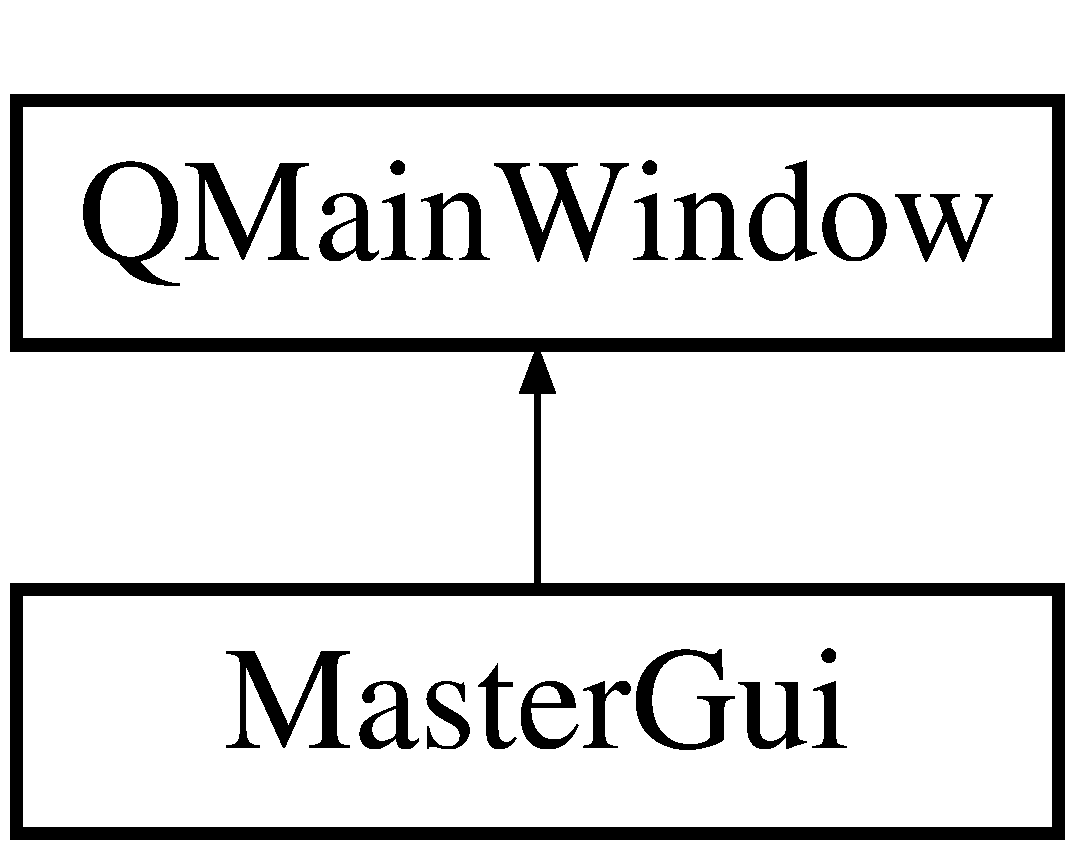
\includegraphics[height=2.000000cm]{class_master_gui}
\end{center}
\end{figure}
\subsection*{Public Member Functions}
\begin{DoxyCompactItemize}
\item 
\hyperlink{class_master_gui_a9d3221a5d6791ffab353e038452e8b79}{Master\-Gui} (Q\-Main\-Window $\ast$parent=0)
\item 
void \hyperlink{class_master_gui_aa8cb5efc03f304d4a80d0d743a30e5b3}{init\-Tool\-Bars} ()
\item 
void \hyperlink{class_master_gui_a65f7212a54b92bdd21498478b9689631}{init\-Menus} ()
\item 
void \hyperlink{class_master_gui_a266df8320dd219d029630f4439c8ceca}{load\-Style} (Q\-String $\ast$style=new Q\-String(\char`\"{}./src/qss/Vanilla.\-css\char`\"{}))
\item 
void \hyperlink{class_master_gui_a4ee6b41a4beb5adfd5c2c15e2490384e}{set\-File\-Menu\-Ptr} (Q\-Menu $\ast$\hyperlink{class_master_gui_a1d768ad74ddb657928df8539c356abb6}{file\-Menu\-Ptr})
\item 
Q\-Menu $\ast$ \hyperlink{class_master_gui_a91a38d0a69249c1f2d6a6175e9fb5342}{get\-File\-Menu\-Ptr} ()
\item 
void \hyperlink{class_master_gui_a91cccfac6fdcd723b4d127a0a668adc7}{set\-Edit\-Menu\-Ptr} (Q\-Menu $\ast$\hyperlink{class_master_gui_aeb708f257518fb47d567d1130bfc7f7f}{edit\-Menu\-Ptr})
\item 
Q\-Menu $\ast$ \hyperlink{class_master_gui_a50196fb1473d723bc940c54879ef6388}{get\-Edit\-Menu\-Ptr} ()
\item 
void \hyperlink{class_master_gui_a4a18f80bfecff6ff5bae16721044dcac}{set\-View\-Menu\-Ptr} (Q\-Menu $\ast$\hyperlink{class_master_gui_acb6a42ddb59a05f60ab7aa2a9fdddbc8}{view\-Menu\-Ptr})
\item 
Q\-Menu $\ast$ \hyperlink{class_master_gui_a3fb03d1a102443e480594a5823917e1a}{get\-View\-Menu\-Ptr} ()
\item 
void \hyperlink{class_master_gui_a2479e3fe7c83858e517855dededf2c51}{set\-Navigate\-Menu\-Ptr} (Q\-Menu $\ast$\hyperlink{class_master_gui_aec75bd894b1c0eecea35c67ecdfcf1b0}{navigate\-Menu\-Ptr})
\item 
Q\-Menu $\ast$ \hyperlink{class_master_gui_a72fd20d98b2d2754fe37beb40e4f5bc6}{get\-Navigate\-Menu\-Ptr} ()
\item 
void \hyperlink{class_master_gui_a58264652e48e97b3313819f0f67bb19e}{set\-Source\-Menu\-Ptr} (Q\-Menu $\ast$\hyperlink{class_master_gui_a3ffd8337f87c7c6eca6b4740fa8d1c57}{source\-Menu\-Ptr})
\item 
Q\-Menu $\ast$ \hyperlink{class_master_gui_ab3b214293b67475e58c899a0683c4b52}{get\-Source\-Menu\-Ptr} ()
\item 
void \hyperlink{class_master_gui_a63c4e2fc02d8101c5d2113783dc86449}{set\-Refactor\-Menu\-Ptr} (Q\-Menu $\ast$\hyperlink{class_master_gui_a44e789008fcc276a7a4294beb98d02c7}{refactor\-Menu\-Ptr})
\item 
Q\-Menu $\ast$ \hyperlink{class_master_gui_a53f1c9667111f13cf966c6eb9d0c6ebf}{get\-Refactor\-Menu\-Ptr} ()
\item 
void \hyperlink{class_master_gui_a9d5a2185276d6a2a7a62227b55e9c8be}{set\-Run\-Menu\-Ptr} (Q\-Menu $\ast$\hyperlink{class_master_gui_ae5b13b338972e99f29e623d258088b07}{run\-Menu\-Ptr})
\item 
Q\-Menu $\ast$ \hyperlink{class_master_gui_a1f42aebf18ac8c07ffcd057bd5bbe22b}{get\-Run\-Menu\-Ptr} ()
\item 
void \hyperlink{class_master_gui_ae43df54970c7b84ed577ac04d593e6f9}{set\-Debug\-Menu\-Ptr} (Q\-Menu $\ast$\hyperlink{class_master_gui_ac1efdb45cdde47584625a8026166c316}{debug\-Menu\-Ptr})
\item 
Q\-Menu $\ast$ \hyperlink{class_master_gui_af9af9881ddfbae0aa41c0a7c4095ac21}{get\-Debug\-Menu\-Ptr} ()
\item 
void \hyperlink{class_master_gui_ae4baf92ceb9abc180d12d133199780cd}{set\-Profile\-Menu\-Ptr} (Q\-Menu $\ast$\hyperlink{class_master_gui_a9c0ef6beee1cb9afcfff786bc4c6bd06}{profile\-Menu\-Ptr})
\item 
Q\-Menu $\ast$ \hyperlink{class_master_gui_a5d529e740085f8db54937ee0c50a40b3}{get\-Profile\-Menu\-Ptr} ()
\item 
void \hyperlink{class_master_gui_a06fc56181b6ae4854f3c51172d5672fb}{set\-Team\-Menu\-Ptr} (Q\-Menu $\ast$\hyperlink{class_master_gui_ad1d5b1e487d4695bab91ab0db856d795}{team\-Menu\-Ptr})
\item 
Q\-Menu $\ast$ \hyperlink{class_master_gui_ac65ef2f0b70bf6edf23fe7dfba0c8d94}{get\-Team\-Menu\-Ptr} ()
\item 
void \hyperlink{class_master_gui_a3361c70cc3726e7f91aaf856ab1df816}{set\-Tools\-Menu\-Ptr} (Q\-Menu $\ast$\hyperlink{class_master_gui_ab751e75ffdf91f5b90b4c2900975f308}{tools\-Menu\-Ptr})
\item 
Q\-Menu $\ast$ \hyperlink{class_master_gui_a8086c7b6829b3bd0cf3eccad2e608f02}{get\-Tools\-Menu\-Ptr} ()
\item 
void \hyperlink{class_master_gui_aea25ff33b56b0111863b5b7af3513a59}{set\-Window\-Menu\-Ptr} (Q\-Menu $\ast$\hyperlink{class_master_gui_ae33b742ac5529096317c8096984ffef1}{window\-Menu\-Ptr})
\item 
Q\-Menu $\ast$ \hyperlink{class_master_gui_a68e66c032b5e7728e0a7e88a04575abc}{get\-Window\-Menu\-Ptr} ()
\item 
void \hyperlink{class_master_gui_a72a4772ee0ff74f6158f99e94c41189a}{set\-Help\-Menu\-Ptr} (Q\-Menu $\ast$\hyperlink{class_master_gui_a4125e9702c79a263642bf83f5f1e2192}{help\-Menu\-Ptr})
\item 
Q\-Menu $\ast$ \hyperlink{class_master_gui_a6eb5ec7778681673520dc9fffd080056}{get\-Help\-Menu\-Ptr} ()
\item 
void \hyperlink{class_master_gui_a83cb5a184a605d368841854ba1cb461b}{set\-Group\-One\-Tool\-Bar\-Ptr} (Q\-Tool\-Bar $\ast$\hyperlink{class_master_gui_a67441e41e16e245976536f18cd7f2d6d}{group\-One\-Tool\-Bar\-Ptr})
\item 
Q\-Tool\-Bar $\ast$ \hyperlink{class_master_gui_a7da1e17d6cfd6254a7b5da4be625e4ff}{get\-Group\-One\-Tool\-Bar\-Ptr} ()
\item 
void \hyperlink{class_master_gui_a677763f96267d87f843c61dff2d7e4ca}{set\-Group\-Two\-Tool\-Bar\-Ptr} (Q\-Tool\-Bar $\ast$\hyperlink{class_master_gui_aa2c7522e568a43f38861795af343bf76}{group\-Two\-Tool\-Bar\-Ptr})
\item 
Q\-Tool\-Bar $\ast$ \hyperlink{class_master_gui_a3559e8ead0441f1bfe9704f023665b44}{get\-Group\-Two\-Tool\-Bar\-Ptr} ()
\item 
void \hyperlink{class_master_gui_a4ee9de81a0827f42423f0c589cd4f1b4}{set\-Group\-Three\-Tool\-Bar\-Ptr} (Q\-Tool\-Bar $\ast$\hyperlink{class_master_gui_af620c7fd8a0903c84581a657d23ef45b}{group\-Three\-Tool\-Bar\-Ptr})
\item 
Q\-Tool\-Bar $\ast$ \hyperlink{class_master_gui_ae60fb73908b05d9f41eb78197163e10f}{get\-Group\-Three\-Tool\-Bar\-Ptr} ()
\item 
void \hyperlink{class_master_gui_a8d3dd60f8b7760d8e50eacd53b32e69a}{set\-South\-Tool\-Bar\-Ptr} (Q\-Tool\-Bar $\ast$\hyperlink{class_master_gui_a4a0234ba347ba345e79eff8c19ba27c8}{south\-Tool\-Bar\-Ptr})
\item 
Q\-Tool\-Bar $\ast$ \hyperlink{class_master_gui_af58b51918353ad37b1a8817098da1140}{get\-South\-Tool\-Bar\-Ptr} ()
\item 
void \hyperlink{class_master_gui_a5e58bb546e83e37dc826405a5bc3e8fe}{set\-East\-Tool\-Bar\-Ptr} (Q\-Tool\-Bar $\ast$\hyperlink{class_master_gui_a289b4db70744b812566a689bf368c37c}{east\-Tool\-Bar\-Ptr})
\item 
Q\-Tool\-Bar $\ast$ \hyperlink{class_master_gui_a88a3c0c4762455d7a4f416fe752b8723}{get\-East\-Tool\-Bar\-Ptr} ()
\item 
void \hyperlink{class_master_gui_a768fa0a0b9cb7886f703b7b60f0b1f57}{set\-West\-Tool\-Bar\-Ptr} (Q\-Tool\-Bar $\ast$\hyperlink{class_master_gui_ad8bf561c56063077e97f9a993fa38ee4}{west\-Tool\-Bar\-Ptr})
\item 
Q\-Tool\-Bar $\ast$ \hyperlink{class_master_gui_a6863200bf96fb94a3afee4696762f259}{get\-West\-Tool\-Bar\-Ptr} ()
\item 
void \hyperlink{class_master_gui_a528332ae24456ea6efddaba74527852b}{set\-Tab\-Widget} (Q\-Tab\-Widget $\ast$\hyperlink{class_master_gui_a3bca8bd4cc4ecef70de27afff52a7b08}{tab\-Widget})
\item 
Q\-Tab\-Widget $\ast$ \hyperlink{class_master_gui_a6dd82c5ecf1ed32a4b67de6d4778b5d8}{get\-Tab\-Widget} ()
\item 
void \hyperlink{class_master_gui_ab468fb7b10a30bf6350bf030ce32a5fa}{set\-Editor} (Q\-Text\-Edit $\ast$\hyperlink{class_master_gui_a0681f0b3d1828d84c0c0cd7e4d765d98}{editor})
\item 
Q\-Text\-Edit $\ast$ \hyperlink{class_master_gui_a1f6fc301c337d7ec0e77425a3b6573c1}{get\-Editor} ()
\item 
void \hyperlink{class_master_gui_aa7ab2e7e8f2a5128eb8b6b14fc569ec4}{set\-Master\-Actions} (\hyperlink{class_master_actions}{Master\-Actions} $\ast$\hyperlink{class_master_gui_a85dc72333d336db18a92207a09db4ce3}{master\-Actions})
\item 
\hyperlink{class_master_actions}{Master\-Actions} $\ast$ \hyperlink{class_master_gui_a529d566a29d89fd686a5f8d37cad8aef}{get\-Master\-Actions} ()
\item 
void \hyperlink{class_master_gui_a355c5dcc87dc16c5bbe5b5917cc54392}{set\-Master\-Tool\-Bars} (\hyperlink{class_master_tool_bars}{Master\-Tool\-Bars} $\ast$\hyperlink{class_master_gui_afb90e8f19dae43cb78c8495e5708e68b}{master\-Tool\-Bars})
\item 
\hyperlink{class_master_tool_bars}{Master\-Tool\-Bars} $\ast$ \hyperlink{class_master_gui_a14e04dcaf7233f6ce5fce47b58e18ef5}{get\-Master\-Tool\-Bars} ()
\item 
void \hyperlink{class_master_gui_a377da4ce23db123d0e2cef68d2409e1d}{set\-Master\-Menus} (\hyperlink{class_master_menus}{Master\-Menus} $\ast$\hyperlink{class_master_gui_a27f793278e486a5bfec69ef366199e5d}{master\-Menus})
\item 
\hyperlink{class_master_menus}{Master\-Menus} $\ast$ \hyperlink{class_master_gui_ab2d15cb4a25f2fb75a10e01e0f93a850}{get\-Master\-Menus} ()
\item 
void \hyperlink{class_master_gui_a76571dfcf6fac7274f39e90d72929564}{set\-Central\-Gui} (\hyperlink{class_central_gui}{Central\-Gui} $\ast$\hyperlink{class_master_gui_a565fc5a3622b8b5417b26dd1306439b8}{central\-Gui})
\item 
\hyperlink{class_central_gui}{Central\-Gui} $\ast$ \hyperlink{class_master_gui_a8672503d8c79f2377f76a04791e56530}{get\-Central\-Gui} ()
\item 
Q\-String $\ast$ \hyperlink{class_master_gui_a96d5da37e4de63a0c0e9d36eb4a53f1e}{to\-String} ()
\item 
\hyperlink{class_master_gui_a4eeae08177c54aba4aad160fc1c5efc6}{$\sim$\-Master\-Gui} ()
\end{DoxyCompactItemize}
\subsection*{Private Attributes}
\begin{DoxyCompactItemize}
\item 
Q\-Menu $\ast$ \hyperlink{class_master_gui_a1d768ad74ddb657928df8539c356abb6}{file\-Menu\-Ptr}
\item 
Q\-Menu $\ast$ \hyperlink{class_master_gui_aeb708f257518fb47d567d1130bfc7f7f}{edit\-Menu\-Ptr}
\item 
Q\-Menu $\ast$ \hyperlink{class_master_gui_acb6a42ddb59a05f60ab7aa2a9fdddbc8}{view\-Menu\-Ptr}
\item 
Q\-Menu $\ast$ \hyperlink{class_master_gui_aec75bd894b1c0eecea35c67ecdfcf1b0}{navigate\-Menu\-Ptr}
\item 
Q\-Menu $\ast$ \hyperlink{class_master_gui_a3ffd8337f87c7c6eca6b4740fa8d1c57}{source\-Menu\-Ptr}
\item 
Q\-Menu $\ast$ \hyperlink{class_master_gui_a44e789008fcc276a7a4294beb98d02c7}{refactor\-Menu\-Ptr}
\item 
Q\-Menu $\ast$ \hyperlink{class_master_gui_ae5b13b338972e99f29e623d258088b07}{run\-Menu\-Ptr}
\item 
Q\-Menu $\ast$ \hyperlink{class_master_gui_ac1efdb45cdde47584625a8026166c316}{debug\-Menu\-Ptr}
\item 
Q\-Menu $\ast$ \hyperlink{class_master_gui_a9c0ef6beee1cb9afcfff786bc4c6bd06}{profile\-Menu\-Ptr}
\item 
Q\-Menu $\ast$ \hyperlink{class_master_gui_ad1d5b1e487d4695bab91ab0db856d795}{team\-Menu\-Ptr}
\item 
Q\-Menu $\ast$ \hyperlink{class_master_gui_ab751e75ffdf91f5b90b4c2900975f308}{tools\-Menu\-Ptr}
\item 
Q\-Menu $\ast$ \hyperlink{class_master_gui_ae33b742ac5529096317c8096984ffef1}{window\-Menu\-Ptr}
\item 
Q\-Menu $\ast$ \hyperlink{class_master_gui_a4125e9702c79a263642bf83f5f1e2192}{help\-Menu\-Ptr}
\item 
Q\-Tool\-Bar $\ast$ \hyperlink{class_master_gui_a67441e41e16e245976536f18cd7f2d6d}{group\-One\-Tool\-Bar\-Ptr}
\item 
Q\-Tool\-Bar $\ast$ \hyperlink{class_master_gui_aa2c7522e568a43f38861795af343bf76}{group\-Two\-Tool\-Bar\-Ptr}
\item 
Q\-Tool\-Bar $\ast$ \hyperlink{class_master_gui_af620c7fd8a0903c84581a657d23ef45b}{group\-Three\-Tool\-Bar\-Ptr}
\item 
Q\-Tool\-Bar $\ast$ \hyperlink{class_master_gui_a4a0234ba347ba345e79eff8c19ba27c8}{south\-Tool\-Bar\-Ptr}
\item 
Q\-Tool\-Bar $\ast$ \hyperlink{class_master_gui_a289b4db70744b812566a689bf368c37c}{east\-Tool\-Bar\-Ptr}
\item 
Q\-Tool\-Bar $\ast$ \hyperlink{class_master_gui_ad8bf561c56063077e97f9a993fa38ee4}{west\-Tool\-Bar\-Ptr}
\item 
Q\-Tab\-Widget $\ast$ \hyperlink{class_master_gui_a3bca8bd4cc4ecef70de27afff52a7b08}{tab\-Widget}
\item 
Q\-Text\-Edit $\ast$ \hyperlink{class_master_gui_a0681f0b3d1828d84c0c0cd7e4d765d98}{editor}
\item 
\hyperlink{class_master_actions}{Master\-Actions} $\ast$ \hyperlink{class_master_gui_a85dc72333d336db18a92207a09db4ce3}{master\-Actions}
\item 
\hyperlink{class_master_tool_bars}{Master\-Tool\-Bars} $\ast$ \hyperlink{class_master_gui_afb90e8f19dae43cb78c8495e5708e68b}{master\-Tool\-Bars}
\item 
\hyperlink{class_master_menus}{Master\-Menus} $\ast$ \hyperlink{class_master_gui_a27f793278e486a5bfec69ef366199e5d}{master\-Menus}
\item 
\hyperlink{class_master_status_bar}{Master\-Status\-Bar} $\ast$ \hyperlink{class_master_gui_a69899e3a9712e70d91f42b9d8ba2bd22}{master\-Status\-Bar}
\item 
\hyperlink{class_central_gui}{Central\-Gui} $\ast$ \hyperlink{class_master_gui_a565fc5a3622b8b5417b26dd1306439b8}{central\-Gui}
\end{DoxyCompactItemize}


\subsection{Constructor \& Destructor Documentation}
\hypertarget{class_master_gui_a9d3221a5d6791ffab353e038452e8b79}{\index{Master\-Gui@{Master\-Gui}!Master\-Gui@{Master\-Gui}}
\index{Master\-Gui@{Master\-Gui}!MasterGui@{Master\-Gui}}
\subsubsection[{Master\-Gui}]{\setlength{\rightskip}{0pt plus 5cm}Master\-Gui\-::\-Master\-Gui (
\begin{DoxyParamCaption}
\item[{Q\-Main\-Window $\ast$}]{parent = {\ttfamily 0}}
\end{DoxyParamCaption}
)}}\label{class_master_gui_a9d3221a5d6791ffab353e038452e8b79}
\hypertarget{class_master_gui_a4eeae08177c54aba4aad160fc1c5efc6}{\index{Master\-Gui@{Master\-Gui}!$\sim$\-Master\-Gui@{$\sim$\-Master\-Gui}}
\index{$\sim$\-Master\-Gui@{$\sim$\-Master\-Gui}!MasterGui@{Master\-Gui}}
\subsubsection[{$\sim$\-Master\-Gui}]{\setlength{\rightskip}{0pt plus 5cm}Master\-Gui\-::$\sim$\-Master\-Gui (
\begin{DoxyParamCaption}
{}
\end{DoxyParamCaption}
)}}\label{class_master_gui_a4eeae08177c54aba4aad160fc1c5efc6}


\subsection{Member Function Documentation}
\hypertarget{class_master_gui_a8672503d8c79f2377f76a04791e56530}{\index{Master\-Gui@{Master\-Gui}!get\-Central\-Gui@{get\-Central\-Gui}}
\index{get\-Central\-Gui@{get\-Central\-Gui}!MasterGui@{Master\-Gui}}
\subsubsection[{get\-Central\-Gui}]{\setlength{\rightskip}{0pt plus 5cm}{\bf Central\-Gui} $\ast$ Master\-Gui\-::get\-Central\-Gui (
\begin{DoxyParamCaption}
{}
\end{DoxyParamCaption}
)}}\label{class_master_gui_a8672503d8c79f2377f76a04791e56530}
\hypertarget{class_master_gui_af9af9881ddfbae0aa41c0a7c4095ac21}{\index{Master\-Gui@{Master\-Gui}!get\-Debug\-Menu\-Ptr@{get\-Debug\-Menu\-Ptr}}
\index{get\-Debug\-Menu\-Ptr@{get\-Debug\-Menu\-Ptr}!MasterGui@{Master\-Gui}}
\subsubsection[{get\-Debug\-Menu\-Ptr}]{\setlength{\rightskip}{0pt plus 5cm}Q\-Menu $\ast$ Master\-Gui\-::get\-Debug\-Menu\-Ptr (
\begin{DoxyParamCaption}
{}
\end{DoxyParamCaption}
)}}\label{class_master_gui_af9af9881ddfbae0aa41c0a7c4095ac21}
\hypertarget{class_master_gui_a88a3c0c4762455d7a4f416fe752b8723}{\index{Master\-Gui@{Master\-Gui}!get\-East\-Tool\-Bar\-Ptr@{get\-East\-Tool\-Bar\-Ptr}}
\index{get\-East\-Tool\-Bar\-Ptr@{get\-East\-Tool\-Bar\-Ptr}!MasterGui@{Master\-Gui}}
\subsubsection[{get\-East\-Tool\-Bar\-Ptr}]{\setlength{\rightskip}{0pt plus 5cm}Q\-Tool\-Bar $\ast$ Master\-Gui\-::get\-East\-Tool\-Bar\-Ptr (
\begin{DoxyParamCaption}
{}
\end{DoxyParamCaption}
)}}\label{class_master_gui_a88a3c0c4762455d7a4f416fe752b8723}
\hypertarget{class_master_gui_a50196fb1473d723bc940c54879ef6388}{\index{Master\-Gui@{Master\-Gui}!get\-Edit\-Menu\-Ptr@{get\-Edit\-Menu\-Ptr}}
\index{get\-Edit\-Menu\-Ptr@{get\-Edit\-Menu\-Ptr}!MasterGui@{Master\-Gui}}
\subsubsection[{get\-Edit\-Menu\-Ptr}]{\setlength{\rightskip}{0pt plus 5cm}Q\-Menu $\ast$ Master\-Gui\-::get\-Edit\-Menu\-Ptr (
\begin{DoxyParamCaption}
{}
\end{DoxyParamCaption}
)}}\label{class_master_gui_a50196fb1473d723bc940c54879ef6388}
\hypertarget{class_master_gui_a1f6fc301c337d7ec0e77425a3b6573c1}{\index{Master\-Gui@{Master\-Gui}!get\-Editor@{get\-Editor}}
\index{get\-Editor@{get\-Editor}!MasterGui@{Master\-Gui}}
\subsubsection[{get\-Editor}]{\setlength{\rightskip}{0pt plus 5cm}Q\-Text\-Edit $\ast$ Master\-Gui\-::get\-Editor (
\begin{DoxyParamCaption}
{}
\end{DoxyParamCaption}
)}}\label{class_master_gui_a1f6fc301c337d7ec0e77425a3b6573c1}
\hypertarget{class_master_gui_a91a38d0a69249c1f2d6a6175e9fb5342}{\index{Master\-Gui@{Master\-Gui}!get\-File\-Menu\-Ptr@{get\-File\-Menu\-Ptr}}
\index{get\-File\-Menu\-Ptr@{get\-File\-Menu\-Ptr}!MasterGui@{Master\-Gui}}
\subsubsection[{get\-File\-Menu\-Ptr}]{\setlength{\rightskip}{0pt plus 5cm}Q\-Menu $\ast$ Master\-Gui\-::get\-File\-Menu\-Ptr (
\begin{DoxyParamCaption}
{}
\end{DoxyParamCaption}
)}}\label{class_master_gui_a91a38d0a69249c1f2d6a6175e9fb5342}
\hypertarget{class_master_gui_a7da1e17d6cfd6254a7b5da4be625e4ff}{\index{Master\-Gui@{Master\-Gui}!get\-Group\-One\-Tool\-Bar\-Ptr@{get\-Group\-One\-Tool\-Bar\-Ptr}}
\index{get\-Group\-One\-Tool\-Bar\-Ptr@{get\-Group\-One\-Tool\-Bar\-Ptr}!MasterGui@{Master\-Gui}}
\subsubsection[{get\-Group\-One\-Tool\-Bar\-Ptr}]{\setlength{\rightskip}{0pt plus 5cm}Q\-Tool\-Bar $\ast$ Master\-Gui\-::get\-Group\-One\-Tool\-Bar\-Ptr (
\begin{DoxyParamCaption}
{}
\end{DoxyParamCaption}
)}}\label{class_master_gui_a7da1e17d6cfd6254a7b5da4be625e4ff}
\hypertarget{class_master_gui_ae60fb73908b05d9f41eb78197163e10f}{\index{Master\-Gui@{Master\-Gui}!get\-Group\-Three\-Tool\-Bar\-Ptr@{get\-Group\-Three\-Tool\-Bar\-Ptr}}
\index{get\-Group\-Three\-Tool\-Bar\-Ptr@{get\-Group\-Three\-Tool\-Bar\-Ptr}!MasterGui@{Master\-Gui}}
\subsubsection[{get\-Group\-Three\-Tool\-Bar\-Ptr}]{\setlength{\rightskip}{0pt plus 5cm}Q\-Tool\-Bar $\ast$ Master\-Gui\-::get\-Group\-Three\-Tool\-Bar\-Ptr (
\begin{DoxyParamCaption}
{}
\end{DoxyParamCaption}
)}}\label{class_master_gui_ae60fb73908b05d9f41eb78197163e10f}
\hypertarget{class_master_gui_a3559e8ead0441f1bfe9704f023665b44}{\index{Master\-Gui@{Master\-Gui}!get\-Group\-Two\-Tool\-Bar\-Ptr@{get\-Group\-Two\-Tool\-Bar\-Ptr}}
\index{get\-Group\-Two\-Tool\-Bar\-Ptr@{get\-Group\-Two\-Tool\-Bar\-Ptr}!MasterGui@{Master\-Gui}}
\subsubsection[{get\-Group\-Two\-Tool\-Bar\-Ptr}]{\setlength{\rightskip}{0pt plus 5cm}Q\-Tool\-Bar $\ast$ Master\-Gui\-::get\-Group\-Two\-Tool\-Bar\-Ptr (
\begin{DoxyParamCaption}
{}
\end{DoxyParamCaption}
)}}\label{class_master_gui_a3559e8ead0441f1bfe9704f023665b44}
\hypertarget{class_master_gui_a6eb5ec7778681673520dc9fffd080056}{\index{Master\-Gui@{Master\-Gui}!get\-Help\-Menu\-Ptr@{get\-Help\-Menu\-Ptr}}
\index{get\-Help\-Menu\-Ptr@{get\-Help\-Menu\-Ptr}!MasterGui@{Master\-Gui}}
\subsubsection[{get\-Help\-Menu\-Ptr}]{\setlength{\rightskip}{0pt plus 5cm}Q\-Menu $\ast$ Master\-Gui\-::get\-Help\-Menu\-Ptr (
\begin{DoxyParamCaption}
{}
\end{DoxyParamCaption}
)}}\label{class_master_gui_a6eb5ec7778681673520dc9fffd080056}
\hypertarget{class_master_gui_a529d566a29d89fd686a5f8d37cad8aef}{\index{Master\-Gui@{Master\-Gui}!get\-Master\-Actions@{get\-Master\-Actions}}
\index{get\-Master\-Actions@{get\-Master\-Actions}!MasterGui@{Master\-Gui}}
\subsubsection[{get\-Master\-Actions}]{\setlength{\rightskip}{0pt plus 5cm}{\bf Master\-Actions} $\ast$ Master\-Gui\-::get\-Master\-Actions (
\begin{DoxyParamCaption}
{}
\end{DoxyParamCaption}
)}}\label{class_master_gui_a529d566a29d89fd686a5f8d37cad8aef}
\hypertarget{class_master_gui_ab2d15cb4a25f2fb75a10e01e0f93a850}{\index{Master\-Gui@{Master\-Gui}!get\-Master\-Menus@{get\-Master\-Menus}}
\index{get\-Master\-Menus@{get\-Master\-Menus}!MasterGui@{Master\-Gui}}
\subsubsection[{get\-Master\-Menus}]{\setlength{\rightskip}{0pt plus 5cm}{\bf Master\-Menus} $\ast$ Master\-Gui\-::get\-Master\-Menus (
\begin{DoxyParamCaption}
{}
\end{DoxyParamCaption}
)}}\label{class_master_gui_ab2d15cb4a25f2fb75a10e01e0f93a850}
\hypertarget{class_master_gui_a14e04dcaf7233f6ce5fce47b58e18ef5}{\index{Master\-Gui@{Master\-Gui}!get\-Master\-Tool\-Bars@{get\-Master\-Tool\-Bars}}
\index{get\-Master\-Tool\-Bars@{get\-Master\-Tool\-Bars}!MasterGui@{Master\-Gui}}
\subsubsection[{get\-Master\-Tool\-Bars}]{\setlength{\rightskip}{0pt plus 5cm}{\bf Master\-Tool\-Bars} $\ast$ Master\-Gui\-::get\-Master\-Tool\-Bars (
\begin{DoxyParamCaption}
{}
\end{DoxyParamCaption}
)}}\label{class_master_gui_a14e04dcaf7233f6ce5fce47b58e18ef5}
\hypertarget{class_master_gui_a72fd20d98b2d2754fe37beb40e4f5bc6}{\index{Master\-Gui@{Master\-Gui}!get\-Navigate\-Menu\-Ptr@{get\-Navigate\-Menu\-Ptr}}
\index{get\-Navigate\-Menu\-Ptr@{get\-Navigate\-Menu\-Ptr}!MasterGui@{Master\-Gui}}
\subsubsection[{get\-Navigate\-Menu\-Ptr}]{\setlength{\rightskip}{0pt plus 5cm}Q\-Menu $\ast$ Master\-Gui\-::get\-Navigate\-Menu\-Ptr (
\begin{DoxyParamCaption}
{}
\end{DoxyParamCaption}
)}}\label{class_master_gui_a72fd20d98b2d2754fe37beb40e4f5bc6}
\hypertarget{class_master_gui_a5d529e740085f8db54937ee0c50a40b3}{\index{Master\-Gui@{Master\-Gui}!get\-Profile\-Menu\-Ptr@{get\-Profile\-Menu\-Ptr}}
\index{get\-Profile\-Menu\-Ptr@{get\-Profile\-Menu\-Ptr}!MasterGui@{Master\-Gui}}
\subsubsection[{get\-Profile\-Menu\-Ptr}]{\setlength{\rightskip}{0pt plus 5cm}Q\-Menu $\ast$ Master\-Gui\-::get\-Profile\-Menu\-Ptr (
\begin{DoxyParamCaption}
{}
\end{DoxyParamCaption}
)}}\label{class_master_gui_a5d529e740085f8db54937ee0c50a40b3}
\hypertarget{class_master_gui_a53f1c9667111f13cf966c6eb9d0c6ebf}{\index{Master\-Gui@{Master\-Gui}!get\-Refactor\-Menu\-Ptr@{get\-Refactor\-Menu\-Ptr}}
\index{get\-Refactor\-Menu\-Ptr@{get\-Refactor\-Menu\-Ptr}!MasterGui@{Master\-Gui}}
\subsubsection[{get\-Refactor\-Menu\-Ptr}]{\setlength{\rightskip}{0pt plus 5cm}Q\-Menu $\ast$ Master\-Gui\-::get\-Refactor\-Menu\-Ptr (
\begin{DoxyParamCaption}
{}
\end{DoxyParamCaption}
)}}\label{class_master_gui_a53f1c9667111f13cf966c6eb9d0c6ebf}
\hypertarget{class_master_gui_a1f42aebf18ac8c07ffcd057bd5bbe22b}{\index{Master\-Gui@{Master\-Gui}!get\-Run\-Menu\-Ptr@{get\-Run\-Menu\-Ptr}}
\index{get\-Run\-Menu\-Ptr@{get\-Run\-Menu\-Ptr}!MasterGui@{Master\-Gui}}
\subsubsection[{get\-Run\-Menu\-Ptr}]{\setlength{\rightskip}{0pt plus 5cm}Q\-Menu $\ast$ Master\-Gui\-::get\-Run\-Menu\-Ptr (
\begin{DoxyParamCaption}
{}
\end{DoxyParamCaption}
)}}\label{class_master_gui_a1f42aebf18ac8c07ffcd057bd5bbe22b}
\hypertarget{class_master_gui_ab3b214293b67475e58c899a0683c4b52}{\index{Master\-Gui@{Master\-Gui}!get\-Source\-Menu\-Ptr@{get\-Source\-Menu\-Ptr}}
\index{get\-Source\-Menu\-Ptr@{get\-Source\-Menu\-Ptr}!MasterGui@{Master\-Gui}}
\subsubsection[{get\-Source\-Menu\-Ptr}]{\setlength{\rightskip}{0pt plus 5cm}Q\-Menu $\ast$ Master\-Gui\-::get\-Source\-Menu\-Ptr (
\begin{DoxyParamCaption}
{}
\end{DoxyParamCaption}
)}}\label{class_master_gui_ab3b214293b67475e58c899a0683c4b52}
\hypertarget{class_master_gui_af58b51918353ad37b1a8817098da1140}{\index{Master\-Gui@{Master\-Gui}!get\-South\-Tool\-Bar\-Ptr@{get\-South\-Tool\-Bar\-Ptr}}
\index{get\-South\-Tool\-Bar\-Ptr@{get\-South\-Tool\-Bar\-Ptr}!MasterGui@{Master\-Gui}}
\subsubsection[{get\-South\-Tool\-Bar\-Ptr}]{\setlength{\rightskip}{0pt plus 5cm}Q\-Tool\-Bar $\ast$ Master\-Gui\-::get\-South\-Tool\-Bar\-Ptr (
\begin{DoxyParamCaption}
{}
\end{DoxyParamCaption}
)}}\label{class_master_gui_af58b51918353ad37b1a8817098da1140}
\hypertarget{class_master_gui_a6dd82c5ecf1ed32a4b67de6d4778b5d8}{\index{Master\-Gui@{Master\-Gui}!get\-Tab\-Widget@{get\-Tab\-Widget}}
\index{get\-Tab\-Widget@{get\-Tab\-Widget}!MasterGui@{Master\-Gui}}
\subsubsection[{get\-Tab\-Widget}]{\setlength{\rightskip}{0pt plus 5cm}Q\-Tab\-Widget $\ast$ Master\-Gui\-::get\-Tab\-Widget (
\begin{DoxyParamCaption}
{}
\end{DoxyParamCaption}
)}}\label{class_master_gui_a6dd82c5ecf1ed32a4b67de6d4778b5d8}
\hypertarget{class_master_gui_ac65ef2f0b70bf6edf23fe7dfba0c8d94}{\index{Master\-Gui@{Master\-Gui}!get\-Team\-Menu\-Ptr@{get\-Team\-Menu\-Ptr}}
\index{get\-Team\-Menu\-Ptr@{get\-Team\-Menu\-Ptr}!MasterGui@{Master\-Gui}}
\subsubsection[{get\-Team\-Menu\-Ptr}]{\setlength{\rightskip}{0pt plus 5cm}Q\-Menu $\ast$ Master\-Gui\-::get\-Team\-Menu\-Ptr (
\begin{DoxyParamCaption}
{}
\end{DoxyParamCaption}
)}}\label{class_master_gui_ac65ef2f0b70bf6edf23fe7dfba0c8d94}
\hypertarget{class_master_gui_a8086c7b6829b3bd0cf3eccad2e608f02}{\index{Master\-Gui@{Master\-Gui}!get\-Tools\-Menu\-Ptr@{get\-Tools\-Menu\-Ptr}}
\index{get\-Tools\-Menu\-Ptr@{get\-Tools\-Menu\-Ptr}!MasterGui@{Master\-Gui}}
\subsubsection[{get\-Tools\-Menu\-Ptr}]{\setlength{\rightskip}{0pt plus 5cm}Q\-Menu $\ast$ Master\-Gui\-::get\-Tools\-Menu\-Ptr (
\begin{DoxyParamCaption}
{}
\end{DoxyParamCaption}
)}}\label{class_master_gui_a8086c7b6829b3bd0cf3eccad2e608f02}
\hypertarget{class_master_gui_a3fb03d1a102443e480594a5823917e1a}{\index{Master\-Gui@{Master\-Gui}!get\-View\-Menu\-Ptr@{get\-View\-Menu\-Ptr}}
\index{get\-View\-Menu\-Ptr@{get\-View\-Menu\-Ptr}!MasterGui@{Master\-Gui}}
\subsubsection[{get\-View\-Menu\-Ptr}]{\setlength{\rightskip}{0pt plus 5cm}Q\-Menu $\ast$ Master\-Gui\-::get\-View\-Menu\-Ptr (
\begin{DoxyParamCaption}
{}
\end{DoxyParamCaption}
)}}\label{class_master_gui_a3fb03d1a102443e480594a5823917e1a}
\hypertarget{class_master_gui_a6863200bf96fb94a3afee4696762f259}{\index{Master\-Gui@{Master\-Gui}!get\-West\-Tool\-Bar\-Ptr@{get\-West\-Tool\-Bar\-Ptr}}
\index{get\-West\-Tool\-Bar\-Ptr@{get\-West\-Tool\-Bar\-Ptr}!MasterGui@{Master\-Gui}}
\subsubsection[{get\-West\-Tool\-Bar\-Ptr}]{\setlength{\rightskip}{0pt plus 5cm}Q\-Tool\-Bar $\ast$ Master\-Gui\-::get\-West\-Tool\-Bar\-Ptr (
\begin{DoxyParamCaption}
{}
\end{DoxyParamCaption}
)}}\label{class_master_gui_a6863200bf96fb94a3afee4696762f259}
\hypertarget{class_master_gui_a68e66c032b5e7728e0a7e88a04575abc}{\index{Master\-Gui@{Master\-Gui}!get\-Window\-Menu\-Ptr@{get\-Window\-Menu\-Ptr}}
\index{get\-Window\-Menu\-Ptr@{get\-Window\-Menu\-Ptr}!MasterGui@{Master\-Gui}}
\subsubsection[{get\-Window\-Menu\-Ptr}]{\setlength{\rightskip}{0pt plus 5cm}Q\-Menu $\ast$ Master\-Gui\-::get\-Window\-Menu\-Ptr (
\begin{DoxyParamCaption}
{}
\end{DoxyParamCaption}
)}}\label{class_master_gui_a68e66c032b5e7728e0a7e88a04575abc}
\hypertarget{class_master_gui_a65f7212a54b92bdd21498478b9689631}{\index{Master\-Gui@{Master\-Gui}!init\-Menus@{init\-Menus}}
\index{init\-Menus@{init\-Menus}!MasterGui@{Master\-Gui}}
\subsubsection[{init\-Menus}]{\setlength{\rightskip}{0pt plus 5cm}void Master\-Gui\-::init\-Menus (
\begin{DoxyParamCaption}
{}
\end{DoxyParamCaption}
)}}\label{class_master_gui_a65f7212a54b92bdd21498478b9689631}
\hypertarget{class_master_gui_aa8cb5efc03f304d4a80d0d743a30e5b3}{\index{Master\-Gui@{Master\-Gui}!init\-Tool\-Bars@{init\-Tool\-Bars}}
\index{init\-Tool\-Bars@{init\-Tool\-Bars}!MasterGui@{Master\-Gui}}
\subsubsection[{init\-Tool\-Bars}]{\setlength{\rightskip}{0pt plus 5cm}void Master\-Gui\-::init\-Tool\-Bars (
\begin{DoxyParamCaption}
{}
\end{DoxyParamCaption}
)}}\label{class_master_gui_aa8cb5efc03f304d4a80d0d743a30e5b3}
\hypertarget{class_master_gui_a266df8320dd219d029630f4439c8ceca}{\index{Master\-Gui@{Master\-Gui}!load\-Style@{load\-Style}}
\index{load\-Style@{load\-Style}!MasterGui@{Master\-Gui}}
\subsubsection[{load\-Style}]{\setlength{\rightskip}{0pt plus 5cm}void Master\-Gui\-::load\-Style (
\begin{DoxyParamCaption}
\item[{Q\-String $\ast$}]{style = {\ttfamily new~QString(\char`\"{}./src/qss/Vanilla.css\char`\"{})}}
\end{DoxyParamCaption}
)}}\label{class_master_gui_a266df8320dd219d029630f4439c8ceca}
\hypertarget{class_master_gui_a76571dfcf6fac7274f39e90d72929564}{\index{Master\-Gui@{Master\-Gui}!set\-Central\-Gui@{set\-Central\-Gui}}
\index{set\-Central\-Gui@{set\-Central\-Gui}!MasterGui@{Master\-Gui}}
\subsubsection[{set\-Central\-Gui}]{\setlength{\rightskip}{0pt plus 5cm}void Master\-Gui\-::set\-Central\-Gui (
\begin{DoxyParamCaption}
\item[{{\bf Central\-Gui} $\ast$}]{central\-Gui}
\end{DoxyParamCaption}
)}}\label{class_master_gui_a76571dfcf6fac7274f39e90d72929564}
\hypertarget{class_master_gui_ae43df54970c7b84ed577ac04d593e6f9}{\index{Master\-Gui@{Master\-Gui}!set\-Debug\-Menu\-Ptr@{set\-Debug\-Menu\-Ptr}}
\index{set\-Debug\-Menu\-Ptr@{set\-Debug\-Menu\-Ptr}!MasterGui@{Master\-Gui}}
\subsubsection[{set\-Debug\-Menu\-Ptr}]{\setlength{\rightskip}{0pt plus 5cm}void Master\-Gui\-::set\-Debug\-Menu\-Ptr (
\begin{DoxyParamCaption}
\item[{Q\-Menu $\ast$}]{debug\-Menu\-Ptr}
\end{DoxyParamCaption}
)}}\label{class_master_gui_ae43df54970c7b84ed577ac04d593e6f9}
\hypertarget{class_master_gui_a5e58bb546e83e37dc826405a5bc3e8fe}{\index{Master\-Gui@{Master\-Gui}!set\-East\-Tool\-Bar\-Ptr@{set\-East\-Tool\-Bar\-Ptr}}
\index{set\-East\-Tool\-Bar\-Ptr@{set\-East\-Tool\-Bar\-Ptr}!MasterGui@{Master\-Gui}}
\subsubsection[{set\-East\-Tool\-Bar\-Ptr}]{\setlength{\rightskip}{0pt plus 5cm}void Master\-Gui\-::set\-East\-Tool\-Bar\-Ptr (
\begin{DoxyParamCaption}
\item[{Q\-Tool\-Bar $\ast$}]{east\-Tool\-Bar\-Ptr}
\end{DoxyParamCaption}
)}}\label{class_master_gui_a5e58bb546e83e37dc826405a5bc3e8fe}
\hypertarget{class_master_gui_a91cccfac6fdcd723b4d127a0a668adc7}{\index{Master\-Gui@{Master\-Gui}!set\-Edit\-Menu\-Ptr@{set\-Edit\-Menu\-Ptr}}
\index{set\-Edit\-Menu\-Ptr@{set\-Edit\-Menu\-Ptr}!MasterGui@{Master\-Gui}}
\subsubsection[{set\-Edit\-Menu\-Ptr}]{\setlength{\rightskip}{0pt plus 5cm}void Master\-Gui\-::set\-Edit\-Menu\-Ptr (
\begin{DoxyParamCaption}
\item[{Q\-Menu $\ast$}]{edit\-Menu\-Ptr}
\end{DoxyParamCaption}
)}}\label{class_master_gui_a91cccfac6fdcd723b4d127a0a668adc7}
\hypertarget{class_master_gui_ab468fb7b10a30bf6350bf030ce32a5fa}{\index{Master\-Gui@{Master\-Gui}!set\-Editor@{set\-Editor}}
\index{set\-Editor@{set\-Editor}!MasterGui@{Master\-Gui}}
\subsubsection[{set\-Editor}]{\setlength{\rightskip}{0pt plus 5cm}void Master\-Gui\-::set\-Editor (
\begin{DoxyParamCaption}
\item[{Q\-Text\-Edit $\ast$}]{editor}
\end{DoxyParamCaption}
)}}\label{class_master_gui_ab468fb7b10a30bf6350bf030ce32a5fa}
\hypertarget{class_master_gui_a4ee6b41a4beb5adfd5c2c15e2490384e}{\index{Master\-Gui@{Master\-Gui}!set\-File\-Menu\-Ptr@{set\-File\-Menu\-Ptr}}
\index{set\-File\-Menu\-Ptr@{set\-File\-Menu\-Ptr}!MasterGui@{Master\-Gui}}
\subsubsection[{set\-File\-Menu\-Ptr}]{\setlength{\rightskip}{0pt plus 5cm}void Master\-Gui\-::set\-File\-Menu\-Ptr (
\begin{DoxyParamCaption}
\item[{Q\-Menu $\ast$}]{file\-Menu\-Ptr}
\end{DoxyParamCaption}
)}}\label{class_master_gui_a4ee6b41a4beb5adfd5c2c15e2490384e}
\hypertarget{class_master_gui_a83cb5a184a605d368841854ba1cb461b}{\index{Master\-Gui@{Master\-Gui}!set\-Group\-One\-Tool\-Bar\-Ptr@{set\-Group\-One\-Tool\-Bar\-Ptr}}
\index{set\-Group\-One\-Tool\-Bar\-Ptr@{set\-Group\-One\-Tool\-Bar\-Ptr}!MasterGui@{Master\-Gui}}
\subsubsection[{set\-Group\-One\-Tool\-Bar\-Ptr}]{\setlength{\rightskip}{0pt plus 5cm}void Master\-Gui\-::set\-Group\-One\-Tool\-Bar\-Ptr (
\begin{DoxyParamCaption}
\item[{Q\-Tool\-Bar $\ast$}]{group\-One\-Tool\-Bar\-Ptr}
\end{DoxyParamCaption}
)}}\label{class_master_gui_a83cb5a184a605d368841854ba1cb461b}
\hypertarget{class_master_gui_a4ee9de81a0827f42423f0c589cd4f1b4}{\index{Master\-Gui@{Master\-Gui}!set\-Group\-Three\-Tool\-Bar\-Ptr@{set\-Group\-Three\-Tool\-Bar\-Ptr}}
\index{set\-Group\-Three\-Tool\-Bar\-Ptr@{set\-Group\-Three\-Tool\-Bar\-Ptr}!MasterGui@{Master\-Gui}}
\subsubsection[{set\-Group\-Three\-Tool\-Bar\-Ptr}]{\setlength{\rightskip}{0pt plus 5cm}void Master\-Gui\-::set\-Group\-Three\-Tool\-Bar\-Ptr (
\begin{DoxyParamCaption}
\item[{Q\-Tool\-Bar $\ast$}]{group\-Three\-Tool\-Bar\-Ptr}
\end{DoxyParamCaption}
)}}\label{class_master_gui_a4ee9de81a0827f42423f0c589cd4f1b4}
\hypertarget{class_master_gui_a677763f96267d87f843c61dff2d7e4ca}{\index{Master\-Gui@{Master\-Gui}!set\-Group\-Two\-Tool\-Bar\-Ptr@{set\-Group\-Two\-Tool\-Bar\-Ptr}}
\index{set\-Group\-Two\-Tool\-Bar\-Ptr@{set\-Group\-Two\-Tool\-Bar\-Ptr}!MasterGui@{Master\-Gui}}
\subsubsection[{set\-Group\-Two\-Tool\-Bar\-Ptr}]{\setlength{\rightskip}{0pt plus 5cm}void Master\-Gui\-::set\-Group\-Two\-Tool\-Bar\-Ptr (
\begin{DoxyParamCaption}
\item[{Q\-Tool\-Bar $\ast$}]{group\-Two\-Tool\-Bar\-Ptr}
\end{DoxyParamCaption}
)}}\label{class_master_gui_a677763f96267d87f843c61dff2d7e4ca}
\hypertarget{class_master_gui_a72a4772ee0ff74f6158f99e94c41189a}{\index{Master\-Gui@{Master\-Gui}!set\-Help\-Menu\-Ptr@{set\-Help\-Menu\-Ptr}}
\index{set\-Help\-Menu\-Ptr@{set\-Help\-Menu\-Ptr}!MasterGui@{Master\-Gui}}
\subsubsection[{set\-Help\-Menu\-Ptr}]{\setlength{\rightskip}{0pt plus 5cm}void Master\-Gui\-::set\-Help\-Menu\-Ptr (
\begin{DoxyParamCaption}
\item[{Q\-Menu $\ast$}]{help\-Menu\-Ptr}
\end{DoxyParamCaption}
)}}\label{class_master_gui_a72a4772ee0ff74f6158f99e94c41189a}
\hypertarget{class_master_gui_aa7ab2e7e8f2a5128eb8b6b14fc569ec4}{\index{Master\-Gui@{Master\-Gui}!set\-Master\-Actions@{set\-Master\-Actions}}
\index{set\-Master\-Actions@{set\-Master\-Actions}!MasterGui@{Master\-Gui}}
\subsubsection[{set\-Master\-Actions}]{\setlength{\rightskip}{0pt plus 5cm}void Master\-Gui\-::set\-Master\-Actions (
\begin{DoxyParamCaption}
\item[{{\bf Master\-Actions} $\ast$}]{master\-Actions}
\end{DoxyParamCaption}
)}}\label{class_master_gui_aa7ab2e7e8f2a5128eb8b6b14fc569ec4}
\hypertarget{class_master_gui_a377da4ce23db123d0e2cef68d2409e1d}{\index{Master\-Gui@{Master\-Gui}!set\-Master\-Menus@{set\-Master\-Menus}}
\index{set\-Master\-Menus@{set\-Master\-Menus}!MasterGui@{Master\-Gui}}
\subsubsection[{set\-Master\-Menus}]{\setlength{\rightskip}{0pt plus 5cm}void Master\-Gui\-::set\-Master\-Menus (
\begin{DoxyParamCaption}
\item[{{\bf Master\-Menus} $\ast$}]{master\-Menus}
\end{DoxyParamCaption}
)}}\label{class_master_gui_a377da4ce23db123d0e2cef68d2409e1d}
\hypertarget{class_master_gui_a355c5dcc87dc16c5bbe5b5917cc54392}{\index{Master\-Gui@{Master\-Gui}!set\-Master\-Tool\-Bars@{set\-Master\-Tool\-Bars}}
\index{set\-Master\-Tool\-Bars@{set\-Master\-Tool\-Bars}!MasterGui@{Master\-Gui}}
\subsubsection[{set\-Master\-Tool\-Bars}]{\setlength{\rightskip}{0pt plus 5cm}void Master\-Gui\-::set\-Master\-Tool\-Bars (
\begin{DoxyParamCaption}
\item[{{\bf Master\-Tool\-Bars} $\ast$}]{master\-Tool\-Bars}
\end{DoxyParamCaption}
)}}\label{class_master_gui_a355c5dcc87dc16c5bbe5b5917cc54392}
\hypertarget{class_master_gui_a2479e3fe7c83858e517855dededf2c51}{\index{Master\-Gui@{Master\-Gui}!set\-Navigate\-Menu\-Ptr@{set\-Navigate\-Menu\-Ptr}}
\index{set\-Navigate\-Menu\-Ptr@{set\-Navigate\-Menu\-Ptr}!MasterGui@{Master\-Gui}}
\subsubsection[{set\-Navigate\-Menu\-Ptr}]{\setlength{\rightskip}{0pt plus 5cm}void Master\-Gui\-::set\-Navigate\-Menu\-Ptr (
\begin{DoxyParamCaption}
\item[{Q\-Menu $\ast$}]{navigate\-Menu\-Ptr}
\end{DoxyParamCaption}
)}}\label{class_master_gui_a2479e3fe7c83858e517855dededf2c51}
\hypertarget{class_master_gui_ae4baf92ceb9abc180d12d133199780cd}{\index{Master\-Gui@{Master\-Gui}!set\-Profile\-Menu\-Ptr@{set\-Profile\-Menu\-Ptr}}
\index{set\-Profile\-Menu\-Ptr@{set\-Profile\-Menu\-Ptr}!MasterGui@{Master\-Gui}}
\subsubsection[{set\-Profile\-Menu\-Ptr}]{\setlength{\rightskip}{0pt plus 5cm}void Master\-Gui\-::set\-Profile\-Menu\-Ptr (
\begin{DoxyParamCaption}
\item[{Q\-Menu $\ast$}]{profile\-Menu\-Ptr}
\end{DoxyParamCaption}
)}}\label{class_master_gui_ae4baf92ceb9abc180d12d133199780cd}
\hypertarget{class_master_gui_a63c4e2fc02d8101c5d2113783dc86449}{\index{Master\-Gui@{Master\-Gui}!set\-Refactor\-Menu\-Ptr@{set\-Refactor\-Menu\-Ptr}}
\index{set\-Refactor\-Menu\-Ptr@{set\-Refactor\-Menu\-Ptr}!MasterGui@{Master\-Gui}}
\subsubsection[{set\-Refactor\-Menu\-Ptr}]{\setlength{\rightskip}{0pt plus 5cm}void Master\-Gui\-::set\-Refactor\-Menu\-Ptr (
\begin{DoxyParamCaption}
\item[{Q\-Menu $\ast$}]{refactor\-Menu\-Ptr}
\end{DoxyParamCaption}
)}}\label{class_master_gui_a63c4e2fc02d8101c5d2113783dc86449}
\hypertarget{class_master_gui_a9d5a2185276d6a2a7a62227b55e9c8be}{\index{Master\-Gui@{Master\-Gui}!set\-Run\-Menu\-Ptr@{set\-Run\-Menu\-Ptr}}
\index{set\-Run\-Menu\-Ptr@{set\-Run\-Menu\-Ptr}!MasterGui@{Master\-Gui}}
\subsubsection[{set\-Run\-Menu\-Ptr}]{\setlength{\rightskip}{0pt plus 5cm}void Master\-Gui\-::set\-Run\-Menu\-Ptr (
\begin{DoxyParamCaption}
\item[{Q\-Menu $\ast$}]{run\-Menu\-Ptr}
\end{DoxyParamCaption}
)}}\label{class_master_gui_a9d5a2185276d6a2a7a62227b55e9c8be}
\hypertarget{class_master_gui_a58264652e48e97b3313819f0f67bb19e}{\index{Master\-Gui@{Master\-Gui}!set\-Source\-Menu\-Ptr@{set\-Source\-Menu\-Ptr}}
\index{set\-Source\-Menu\-Ptr@{set\-Source\-Menu\-Ptr}!MasterGui@{Master\-Gui}}
\subsubsection[{set\-Source\-Menu\-Ptr}]{\setlength{\rightskip}{0pt plus 5cm}void Master\-Gui\-::set\-Source\-Menu\-Ptr (
\begin{DoxyParamCaption}
\item[{Q\-Menu $\ast$}]{source\-Menu\-Ptr}
\end{DoxyParamCaption}
)}}\label{class_master_gui_a58264652e48e97b3313819f0f67bb19e}
\hypertarget{class_master_gui_a8d3dd60f8b7760d8e50eacd53b32e69a}{\index{Master\-Gui@{Master\-Gui}!set\-South\-Tool\-Bar\-Ptr@{set\-South\-Tool\-Bar\-Ptr}}
\index{set\-South\-Tool\-Bar\-Ptr@{set\-South\-Tool\-Bar\-Ptr}!MasterGui@{Master\-Gui}}
\subsubsection[{set\-South\-Tool\-Bar\-Ptr}]{\setlength{\rightskip}{0pt plus 5cm}void Master\-Gui\-::set\-South\-Tool\-Bar\-Ptr (
\begin{DoxyParamCaption}
\item[{Q\-Tool\-Bar $\ast$}]{south\-Tool\-Bar\-Ptr}
\end{DoxyParamCaption}
)}}\label{class_master_gui_a8d3dd60f8b7760d8e50eacd53b32e69a}
\hypertarget{class_master_gui_a528332ae24456ea6efddaba74527852b}{\index{Master\-Gui@{Master\-Gui}!set\-Tab\-Widget@{set\-Tab\-Widget}}
\index{set\-Tab\-Widget@{set\-Tab\-Widget}!MasterGui@{Master\-Gui}}
\subsubsection[{set\-Tab\-Widget}]{\setlength{\rightskip}{0pt plus 5cm}void Master\-Gui\-::set\-Tab\-Widget (
\begin{DoxyParamCaption}
\item[{Q\-Tab\-Widget $\ast$}]{tab\-Widget}
\end{DoxyParamCaption}
)}}\label{class_master_gui_a528332ae24456ea6efddaba74527852b}
\hypertarget{class_master_gui_a06fc56181b6ae4854f3c51172d5672fb}{\index{Master\-Gui@{Master\-Gui}!set\-Team\-Menu\-Ptr@{set\-Team\-Menu\-Ptr}}
\index{set\-Team\-Menu\-Ptr@{set\-Team\-Menu\-Ptr}!MasterGui@{Master\-Gui}}
\subsubsection[{set\-Team\-Menu\-Ptr}]{\setlength{\rightskip}{0pt plus 5cm}void Master\-Gui\-::set\-Team\-Menu\-Ptr (
\begin{DoxyParamCaption}
\item[{Q\-Menu $\ast$}]{team\-Menu\-Ptr}
\end{DoxyParamCaption}
)}}\label{class_master_gui_a06fc56181b6ae4854f3c51172d5672fb}
\hypertarget{class_master_gui_a3361c70cc3726e7f91aaf856ab1df816}{\index{Master\-Gui@{Master\-Gui}!set\-Tools\-Menu\-Ptr@{set\-Tools\-Menu\-Ptr}}
\index{set\-Tools\-Menu\-Ptr@{set\-Tools\-Menu\-Ptr}!MasterGui@{Master\-Gui}}
\subsubsection[{set\-Tools\-Menu\-Ptr}]{\setlength{\rightskip}{0pt plus 5cm}void Master\-Gui\-::set\-Tools\-Menu\-Ptr (
\begin{DoxyParamCaption}
\item[{Q\-Menu $\ast$}]{tools\-Menu\-Ptr}
\end{DoxyParamCaption}
)}}\label{class_master_gui_a3361c70cc3726e7f91aaf856ab1df816}
\hypertarget{class_master_gui_a4a18f80bfecff6ff5bae16721044dcac}{\index{Master\-Gui@{Master\-Gui}!set\-View\-Menu\-Ptr@{set\-View\-Menu\-Ptr}}
\index{set\-View\-Menu\-Ptr@{set\-View\-Menu\-Ptr}!MasterGui@{Master\-Gui}}
\subsubsection[{set\-View\-Menu\-Ptr}]{\setlength{\rightskip}{0pt plus 5cm}void Master\-Gui\-::set\-View\-Menu\-Ptr (
\begin{DoxyParamCaption}
\item[{Q\-Menu $\ast$}]{view\-Menu\-Ptr}
\end{DoxyParamCaption}
)}}\label{class_master_gui_a4a18f80bfecff6ff5bae16721044dcac}
\hypertarget{class_master_gui_a768fa0a0b9cb7886f703b7b60f0b1f57}{\index{Master\-Gui@{Master\-Gui}!set\-West\-Tool\-Bar\-Ptr@{set\-West\-Tool\-Bar\-Ptr}}
\index{set\-West\-Tool\-Bar\-Ptr@{set\-West\-Tool\-Bar\-Ptr}!MasterGui@{Master\-Gui}}
\subsubsection[{set\-West\-Tool\-Bar\-Ptr}]{\setlength{\rightskip}{0pt plus 5cm}void Master\-Gui\-::set\-West\-Tool\-Bar\-Ptr (
\begin{DoxyParamCaption}
\item[{Q\-Tool\-Bar $\ast$}]{west\-Tool\-Bar\-Ptr}
\end{DoxyParamCaption}
)}}\label{class_master_gui_a768fa0a0b9cb7886f703b7b60f0b1f57}
\hypertarget{class_master_gui_aea25ff33b56b0111863b5b7af3513a59}{\index{Master\-Gui@{Master\-Gui}!set\-Window\-Menu\-Ptr@{set\-Window\-Menu\-Ptr}}
\index{set\-Window\-Menu\-Ptr@{set\-Window\-Menu\-Ptr}!MasterGui@{Master\-Gui}}
\subsubsection[{set\-Window\-Menu\-Ptr}]{\setlength{\rightskip}{0pt plus 5cm}void Master\-Gui\-::set\-Window\-Menu\-Ptr (
\begin{DoxyParamCaption}
\item[{Q\-Menu $\ast$}]{window\-Menu\-Ptr}
\end{DoxyParamCaption}
)}}\label{class_master_gui_aea25ff33b56b0111863b5b7af3513a59}
\hypertarget{class_master_gui_a96d5da37e4de63a0c0e9d36eb4a53f1e}{\index{Master\-Gui@{Master\-Gui}!to\-String@{to\-String}}
\index{to\-String@{to\-String}!MasterGui@{Master\-Gui}}
\subsubsection[{to\-String}]{\setlength{\rightskip}{0pt plus 5cm}Q\-String $\ast$ Master\-Gui\-::to\-String (
\begin{DoxyParamCaption}
{}
\end{DoxyParamCaption}
)}}\label{class_master_gui_a96d5da37e4de63a0c0e9d36eb4a53f1e}


\subsection{Member Data Documentation}
\hypertarget{class_master_gui_a565fc5a3622b8b5417b26dd1306439b8}{\index{Master\-Gui@{Master\-Gui}!central\-Gui@{central\-Gui}}
\index{central\-Gui@{central\-Gui}!MasterGui@{Master\-Gui}}
\subsubsection[{central\-Gui}]{\setlength{\rightskip}{0pt plus 5cm}{\bf Central\-Gui}$\ast$ Master\-Gui\-::central\-Gui\hspace{0.3cm}{\ttfamily [private]}}}\label{class_master_gui_a565fc5a3622b8b5417b26dd1306439b8}
\hypertarget{class_master_gui_ac1efdb45cdde47584625a8026166c316}{\index{Master\-Gui@{Master\-Gui}!debug\-Menu\-Ptr@{debug\-Menu\-Ptr}}
\index{debug\-Menu\-Ptr@{debug\-Menu\-Ptr}!MasterGui@{Master\-Gui}}
\subsubsection[{debug\-Menu\-Ptr}]{\setlength{\rightskip}{0pt plus 5cm}Q\-Menu$\ast$ Master\-Gui\-::debug\-Menu\-Ptr\hspace{0.3cm}{\ttfamily [private]}}}\label{class_master_gui_ac1efdb45cdde47584625a8026166c316}
\hypertarget{class_master_gui_a289b4db70744b812566a689bf368c37c}{\index{Master\-Gui@{Master\-Gui}!east\-Tool\-Bar\-Ptr@{east\-Tool\-Bar\-Ptr}}
\index{east\-Tool\-Bar\-Ptr@{east\-Tool\-Bar\-Ptr}!MasterGui@{Master\-Gui}}
\subsubsection[{east\-Tool\-Bar\-Ptr}]{\setlength{\rightskip}{0pt plus 5cm}Q\-Tool\-Bar$\ast$ Master\-Gui\-::east\-Tool\-Bar\-Ptr\hspace{0.3cm}{\ttfamily [private]}}}\label{class_master_gui_a289b4db70744b812566a689bf368c37c}
\hypertarget{class_master_gui_aeb708f257518fb47d567d1130bfc7f7f}{\index{Master\-Gui@{Master\-Gui}!edit\-Menu\-Ptr@{edit\-Menu\-Ptr}}
\index{edit\-Menu\-Ptr@{edit\-Menu\-Ptr}!MasterGui@{Master\-Gui}}
\subsubsection[{edit\-Menu\-Ptr}]{\setlength{\rightskip}{0pt plus 5cm}Q\-Menu$\ast$ Master\-Gui\-::edit\-Menu\-Ptr\hspace{0.3cm}{\ttfamily [private]}}}\label{class_master_gui_aeb708f257518fb47d567d1130bfc7f7f}
\hypertarget{class_master_gui_a0681f0b3d1828d84c0c0cd7e4d765d98}{\index{Master\-Gui@{Master\-Gui}!editor@{editor}}
\index{editor@{editor}!MasterGui@{Master\-Gui}}
\subsubsection[{editor}]{\setlength{\rightskip}{0pt plus 5cm}Q\-Text\-Edit$\ast$ Master\-Gui\-::editor\hspace{0.3cm}{\ttfamily [private]}}}\label{class_master_gui_a0681f0b3d1828d84c0c0cd7e4d765d98}
\hypertarget{class_master_gui_a1d768ad74ddb657928df8539c356abb6}{\index{Master\-Gui@{Master\-Gui}!file\-Menu\-Ptr@{file\-Menu\-Ptr}}
\index{file\-Menu\-Ptr@{file\-Menu\-Ptr}!MasterGui@{Master\-Gui}}
\subsubsection[{file\-Menu\-Ptr}]{\setlength{\rightskip}{0pt plus 5cm}Q\-Menu$\ast$ Master\-Gui\-::file\-Menu\-Ptr\hspace{0.3cm}{\ttfamily [private]}}}\label{class_master_gui_a1d768ad74ddb657928df8539c356abb6}
\hypertarget{class_master_gui_a67441e41e16e245976536f18cd7f2d6d}{\index{Master\-Gui@{Master\-Gui}!group\-One\-Tool\-Bar\-Ptr@{group\-One\-Tool\-Bar\-Ptr}}
\index{group\-One\-Tool\-Bar\-Ptr@{group\-One\-Tool\-Bar\-Ptr}!MasterGui@{Master\-Gui}}
\subsubsection[{group\-One\-Tool\-Bar\-Ptr}]{\setlength{\rightskip}{0pt plus 5cm}Q\-Tool\-Bar$\ast$ Master\-Gui\-::group\-One\-Tool\-Bar\-Ptr\hspace{0.3cm}{\ttfamily [private]}}}\label{class_master_gui_a67441e41e16e245976536f18cd7f2d6d}
\hypertarget{class_master_gui_af620c7fd8a0903c84581a657d23ef45b}{\index{Master\-Gui@{Master\-Gui}!group\-Three\-Tool\-Bar\-Ptr@{group\-Three\-Tool\-Bar\-Ptr}}
\index{group\-Three\-Tool\-Bar\-Ptr@{group\-Three\-Tool\-Bar\-Ptr}!MasterGui@{Master\-Gui}}
\subsubsection[{group\-Three\-Tool\-Bar\-Ptr}]{\setlength{\rightskip}{0pt plus 5cm}Q\-Tool\-Bar$\ast$ Master\-Gui\-::group\-Three\-Tool\-Bar\-Ptr\hspace{0.3cm}{\ttfamily [private]}}}\label{class_master_gui_af620c7fd8a0903c84581a657d23ef45b}
\hypertarget{class_master_gui_aa2c7522e568a43f38861795af343bf76}{\index{Master\-Gui@{Master\-Gui}!group\-Two\-Tool\-Bar\-Ptr@{group\-Two\-Tool\-Bar\-Ptr}}
\index{group\-Two\-Tool\-Bar\-Ptr@{group\-Two\-Tool\-Bar\-Ptr}!MasterGui@{Master\-Gui}}
\subsubsection[{group\-Two\-Tool\-Bar\-Ptr}]{\setlength{\rightskip}{0pt plus 5cm}Q\-Tool\-Bar$\ast$ Master\-Gui\-::group\-Two\-Tool\-Bar\-Ptr\hspace{0.3cm}{\ttfamily [private]}}}\label{class_master_gui_aa2c7522e568a43f38861795af343bf76}
\hypertarget{class_master_gui_a4125e9702c79a263642bf83f5f1e2192}{\index{Master\-Gui@{Master\-Gui}!help\-Menu\-Ptr@{help\-Menu\-Ptr}}
\index{help\-Menu\-Ptr@{help\-Menu\-Ptr}!MasterGui@{Master\-Gui}}
\subsubsection[{help\-Menu\-Ptr}]{\setlength{\rightskip}{0pt plus 5cm}Q\-Menu$\ast$ Master\-Gui\-::help\-Menu\-Ptr\hspace{0.3cm}{\ttfamily [private]}}}\label{class_master_gui_a4125e9702c79a263642bf83f5f1e2192}
\hypertarget{class_master_gui_a85dc72333d336db18a92207a09db4ce3}{\index{Master\-Gui@{Master\-Gui}!master\-Actions@{master\-Actions}}
\index{master\-Actions@{master\-Actions}!MasterGui@{Master\-Gui}}
\subsubsection[{master\-Actions}]{\setlength{\rightskip}{0pt plus 5cm}{\bf Master\-Actions}$\ast$ Master\-Gui\-::master\-Actions\hspace{0.3cm}{\ttfamily [private]}}}\label{class_master_gui_a85dc72333d336db18a92207a09db4ce3}
\hypertarget{class_master_gui_a27f793278e486a5bfec69ef366199e5d}{\index{Master\-Gui@{Master\-Gui}!master\-Menus@{master\-Menus}}
\index{master\-Menus@{master\-Menus}!MasterGui@{Master\-Gui}}
\subsubsection[{master\-Menus}]{\setlength{\rightskip}{0pt plus 5cm}{\bf Master\-Menus}$\ast$ Master\-Gui\-::master\-Menus\hspace{0.3cm}{\ttfamily [private]}}}\label{class_master_gui_a27f793278e486a5bfec69ef366199e5d}
\hypertarget{class_master_gui_a69899e3a9712e70d91f42b9d8ba2bd22}{\index{Master\-Gui@{Master\-Gui}!master\-Status\-Bar@{master\-Status\-Bar}}
\index{master\-Status\-Bar@{master\-Status\-Bar}!MasterGui@{Master\-Gui}}
\subsubsection[{master\-Status\-Bar}]{\setlength{\rightskip}{0pt plus 5cm}{\bf Master\-Status\-Bar}$\ast$ Master\-Gui\-::master\-Status\-Bar\hspace{0.3cm}{\ttfamily [private]}}}\label{class_master_gui_a69899e3a9712e70d91f42b9d8ba2bd22}
\hypertarget{class_master_gui_afb90e8f19dae43cb78c8495e5708e68b}{\index{Master\-Gui@{Master\-Gui}!master\-Tool\-Bars@{master\-Tool\-Bars}}
\index{master\-Tool\-Bars@{master\-Tool\-Bars}!MasterGui@{Master\-Gui}}
\subsubsection[{master\-Tool\-Bars}]{\setlength{\rightskip}{0pt plus 5cm}{\bf Master\-Tool\-Bars}$\ast$ Master\-Gui\-::master\-Tool\-Bars\hspace{0.3cm}{\ttfamily [private]}}}\label{class_master_gui_afb90e8f19dae43cb78c8495e5708e68b}
\hypertarget{class_master_gui_aec75bd894b1c0eecea35c67ecdfcf1b0}{\index{Master\-Gui@{Master\-Gui}!navigate\-Menu\-Ptr@{navigate\-Menu\-Ptr}}
\index{navigate\-Menu\-Ptr@{navigate\-Menu\-Ptr}!MasterGui@{Master\-Gui}}
\subsubsection[{navigate\-Menu\-Ptr}]{\setlength{\rightskip}{0pt plus 5cm}Q\-Menu$\ast$ Master\-Gui\-::navigate\-Menu\-Ptr\hspace{0.3cm}{\ttfamily [private]}}}\label{class_master_gui_aec75bd894b1c0eecea35c67ecdfcf1b0}
\hypertarget{class_master_gui_a9c0ef6beee1cb9afcfff786bc4c6bd06}{\index{Master\-Gui@{Master\-Gui}!profile\-Menu\-Ptr@{profile\-Menu\-Ptr}}
\index{profile\-Menu\-Ptr@{profile\-Menu\-Ptr}!MasterGui@{Master\-Gui}}
\subsubsection[{profile\-Menu\-Ptr}]{\setlength{\rightskip}{0pt plus 5cm}Q\-Menu$\ast$ Master\-Gui\-::profile\-Menu\-Ptr\hspace{0.3cm}{\ttfamily [private]}}}\label{class_master_gui_a9c0ef6beee1cb9afcfff786bc4c6bd06}
\hypertarget{class_master_gui_a44e789008fcc276a7a4294beb98d02c7}{\index{Master\-Gui@{Master\-Gui}!refactor\-Menu\-Ptr@{refactor\-Menu\-Ptr}}
\index{refactor\-Menu\-Ptr@{refactor\-Menu\-Ptr}!MasterGui@{Master\-Gui}}
\subsubsection[{refactor\-Menu\-Ptr}]{\setlength{\rightskip}{0pt plus 5cm}Q\-Menu$\ast$ Master\-Gui\-::refactor\-Menu\-Ptr\hspace{0.3cm}{\ttfamily [private]}}}\label{class_master_gui_a44e789008fcc276a7a4294beb98d02c7}
\hypertarget{class_master_gui_ae5b13b338972e99f29e623d258088b07}{\index{Master\-Gui@{Master\-Gui}!run\-Menu\-Ptr@{run\-Menu\-Ptr}}
\index{run\-Menu\-Ptr@{run\-Menu\-Ptr}!MasterGui@{Master\-Gui}}
\subsubsection[{run\-Menu\-Ptr}]{\setlength{\rightskip}{0pt plus 5cm}Q\-Menu$\ast$ Master\-Gui\-::run\-Menu\-Ptr\hspace{0.3cm}{\ttfamily [private]}}}\label{class_master_gui_ae5b13b338972e99f29e623d258088b07}
\hypertarget{class_master_gui_a3ffd8337f87c7c6eca6b4740fa8d1c57}{\index{Master\-Gui@{Master\-Gui}!source\-Menu\-Ptr@{source\-Menu\-Ptr}}
\index{source\-Menu\-Ptr@{source\-Menu\-Ptr}!MasterGui@{Master\-Gui}}
\subsubsection[{source\-Menu\-Ptr}]{\setlength{\rightskip}{0pt plus 5cm}Q\-Menu$\ast$ Master\-Gui\-::source\-Menu\-Ptr\hspace{0.3cm}{\ttfamily [private]}}}\label{class_master_gui_a3ffd8337f87c7c6eca6b4740fa8d1c57}
\hypertarget{class_master_gui_a4a0234ba347ba345e79eff8c19ba27c8}{\index{Master\-Gui@{Master\-Gui}!south\-Tool\-Bar\-Ptr@{south\-Tool\-Bar\-Ptr}}
\index{south\-Tool\-Bar\-Ptr@{south\-Tool\-Bar\-Ptr}!MasterGui@{Master\-Gui}}
\subsubsection[{south\-Tool\-Bar\-Ptr}]{\setlength{\rightskip}{0pt plus 5cm}Q\-Tool\-Bar$\ast$ Master\-Gui\-::south\-Tool\-Bar\-Ptr\hspace{0.3cm}{\ttfamily [private]}}}\label{class_master_gui_a4a0234ba347ba345e79eff8c19ba27c8}
\hypertarget{class_master_gui_a3bca8bd4cc4ecef70de27afff52a7b08}{\index{Master\-Gui@{Master\-Gui}!tab\-Widget@{tab\-Widget}}
\index{tab\-Widget@{tab\-Widget}!MasterGui@{Master\-Gui}}
\subsubsection[{tab\-Widget}]{\setlength{\rightskip}{0pt plus 5cm}Q\-Tab\-Widget$\ast$ Master\-Gui\-::tab\-Widget\hspace{0.3cm}{\ttfamily [private]}}}\label{class_master_gui_a3bca8bd4cc4ecef70de27afff52a7b08}
\hypertarget{class_master_gui_ad1d5b1e487d4695bab91ab0db856d795}{\index{Master\-Gui@{Master\-Gui}!team\-Menu\-Ptr@{team\-Menu\-Ptr}}
\index{team\-Menu\-Ptr@{team\-Menu\-Ptr}!MasterGui@{Master\-Gui}}
\subsubsection[{team\-Menu\-Ptr}]{\setlength{\rightskip}{0pt plus 5cm}Q\-Menu$\ast$ Master\-Gui\-::team\-Menu\-Ptr\hspace{0.3cm}{\ttfamily [private]}}}\label{class_master_gui_ad1d5b1e487d4695bab91ab0db856d795}
\hypertarget{class_master_gui_ab751e75ffdf91f5b90b4c2900975f308}{\index{Master\-Gui@{Master\-Gui}!tools\-Menu\-Ptr@{tools\-Menu\-Ptr}}
\index{tools\-Menu\-Ptr@{tools\-Menu\-Ptr}!MasterGui@{Master\-Gui}}
\subsubsection[{tools\-Menu\-Ptr}]{\setlength{\rightskip}{0pt plus 5cm}Q\-Menu$\ast$ Master\-Gui\-::tools\-Menu\-Ptr\hspace{0.3cm}{\ttfamily [private]}}}\label{class_master_gui_ab751e75ffdf91f5b90b4c2900975f308}
\hypertarget{class_master_gui_acb6a42ddb59a05f60ab7aa2a9fdddbc8}{\index{Master\-Gui@{Master\-Gui}!view\-Menu\-Ptr@{view\-Menu\-Ptr}}
\index{view\-Menu\-Ptr@{view\-Menu\-Ptr}!MasterGui@{Master\-Gui}}
\subsubsection[{view\-Menu\-Ptr}]{\setlength{\rightskip}{0pt plus 5cm}Q\-Menu$\ast$ Master\-Gui\-::view\-Menu\-Ptr\hspace{0.3cm}{\ttfamily [private]}}}\label{class_master_gui_acb6a42ddb59a05f60ab7aa2a9fdddbc8}
\hypertarget{class_master_gui_ad8bf561c56063077e97f9a993fa38ee4}{\index{Master\-Gui@{Master\-Gui}!west\-Tool\-Bar\-Ptr@{west\-Tool\-Bar\-Ptr}}
\index{west\-Tool\-Bar\-Ptr@{west\-Tool\-Bar\-Ptr}!MasterGui@{Master\-Gui}}
\subsubsection[{west\-Tool\-Bar\-Ptr}]{\setlength{\rightskip}{0pt plus 5cm}Q\-Tool\-Bar$\ast$ Master\-Gui\-::west\-Tool\-Bar\-Ptr\hspace{0.3cm}{\ttfamily [private]}}}\label{class_master_gui_ad8bf561c56063077e97f9a993fa38ee4}
\hypertarget{class_master_gui_ae33b742ac5529096317c8096984ffef1}{\index{Master\-Gui@{Master\-Gui}!window\-Menu\-Ptr@{window\-Menu\-Ptr}}
\index{window\-Menu\-Ptr@{window\-Menu\-Ptr}!MasterGui@{Master\-Gui}}
\subsubsection[{window\-Menu\-Ptr}]{\setlength{\rightskip}{0pt plus 5cm}Q\-Menu$\ast$ Master\-Gui\-::window\-Menu\-Ptr\hspace{0.3cm}{\ttfamily [private]}}}\label{class_master_gui_ae33b742ac5529096317c8096984ffef1}


The documentation for this class was generated from the following files\-:\begin{DoxyCompactItemize}
\item 
/home/james/\-Net\-Beans\-Projects/ride/src/\hyperlink{_master_gui_8h}{Master\-Gui.\-h}\item 
/home/james/\-Net\-Beans\-Projects/ride/src/\hyperlink{_master_gui_8cpp}{Master\-Gui.\-cpp}\end{DoxyCompactItemize}

\hypertarget{class_master_menus}{\section{Master\-Menus Class Reference}
\label{class_master_menus}\index{Master\-Menus@{Master\-Menus}}
}


{\ttfamily \#include $<$Master\-Menus.\-h$>$}



Inheritance diagram for Master\-Menus\-:\nopagebreak
\begin{figure}[H]
\begin{center}
\leavevmode
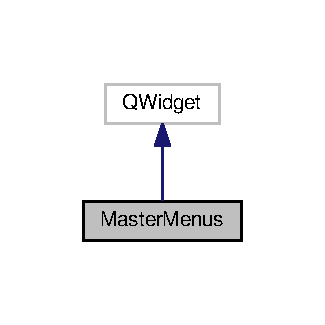
\includegraphics[width=156pt]{class_master_menus__inherit__graph}
\end{center}
\end{figure}


Collaboration diagram for Master\-Menus\-:
\nopagebreak
\begin{figure}[H]
\begin{center}
\leavevmode
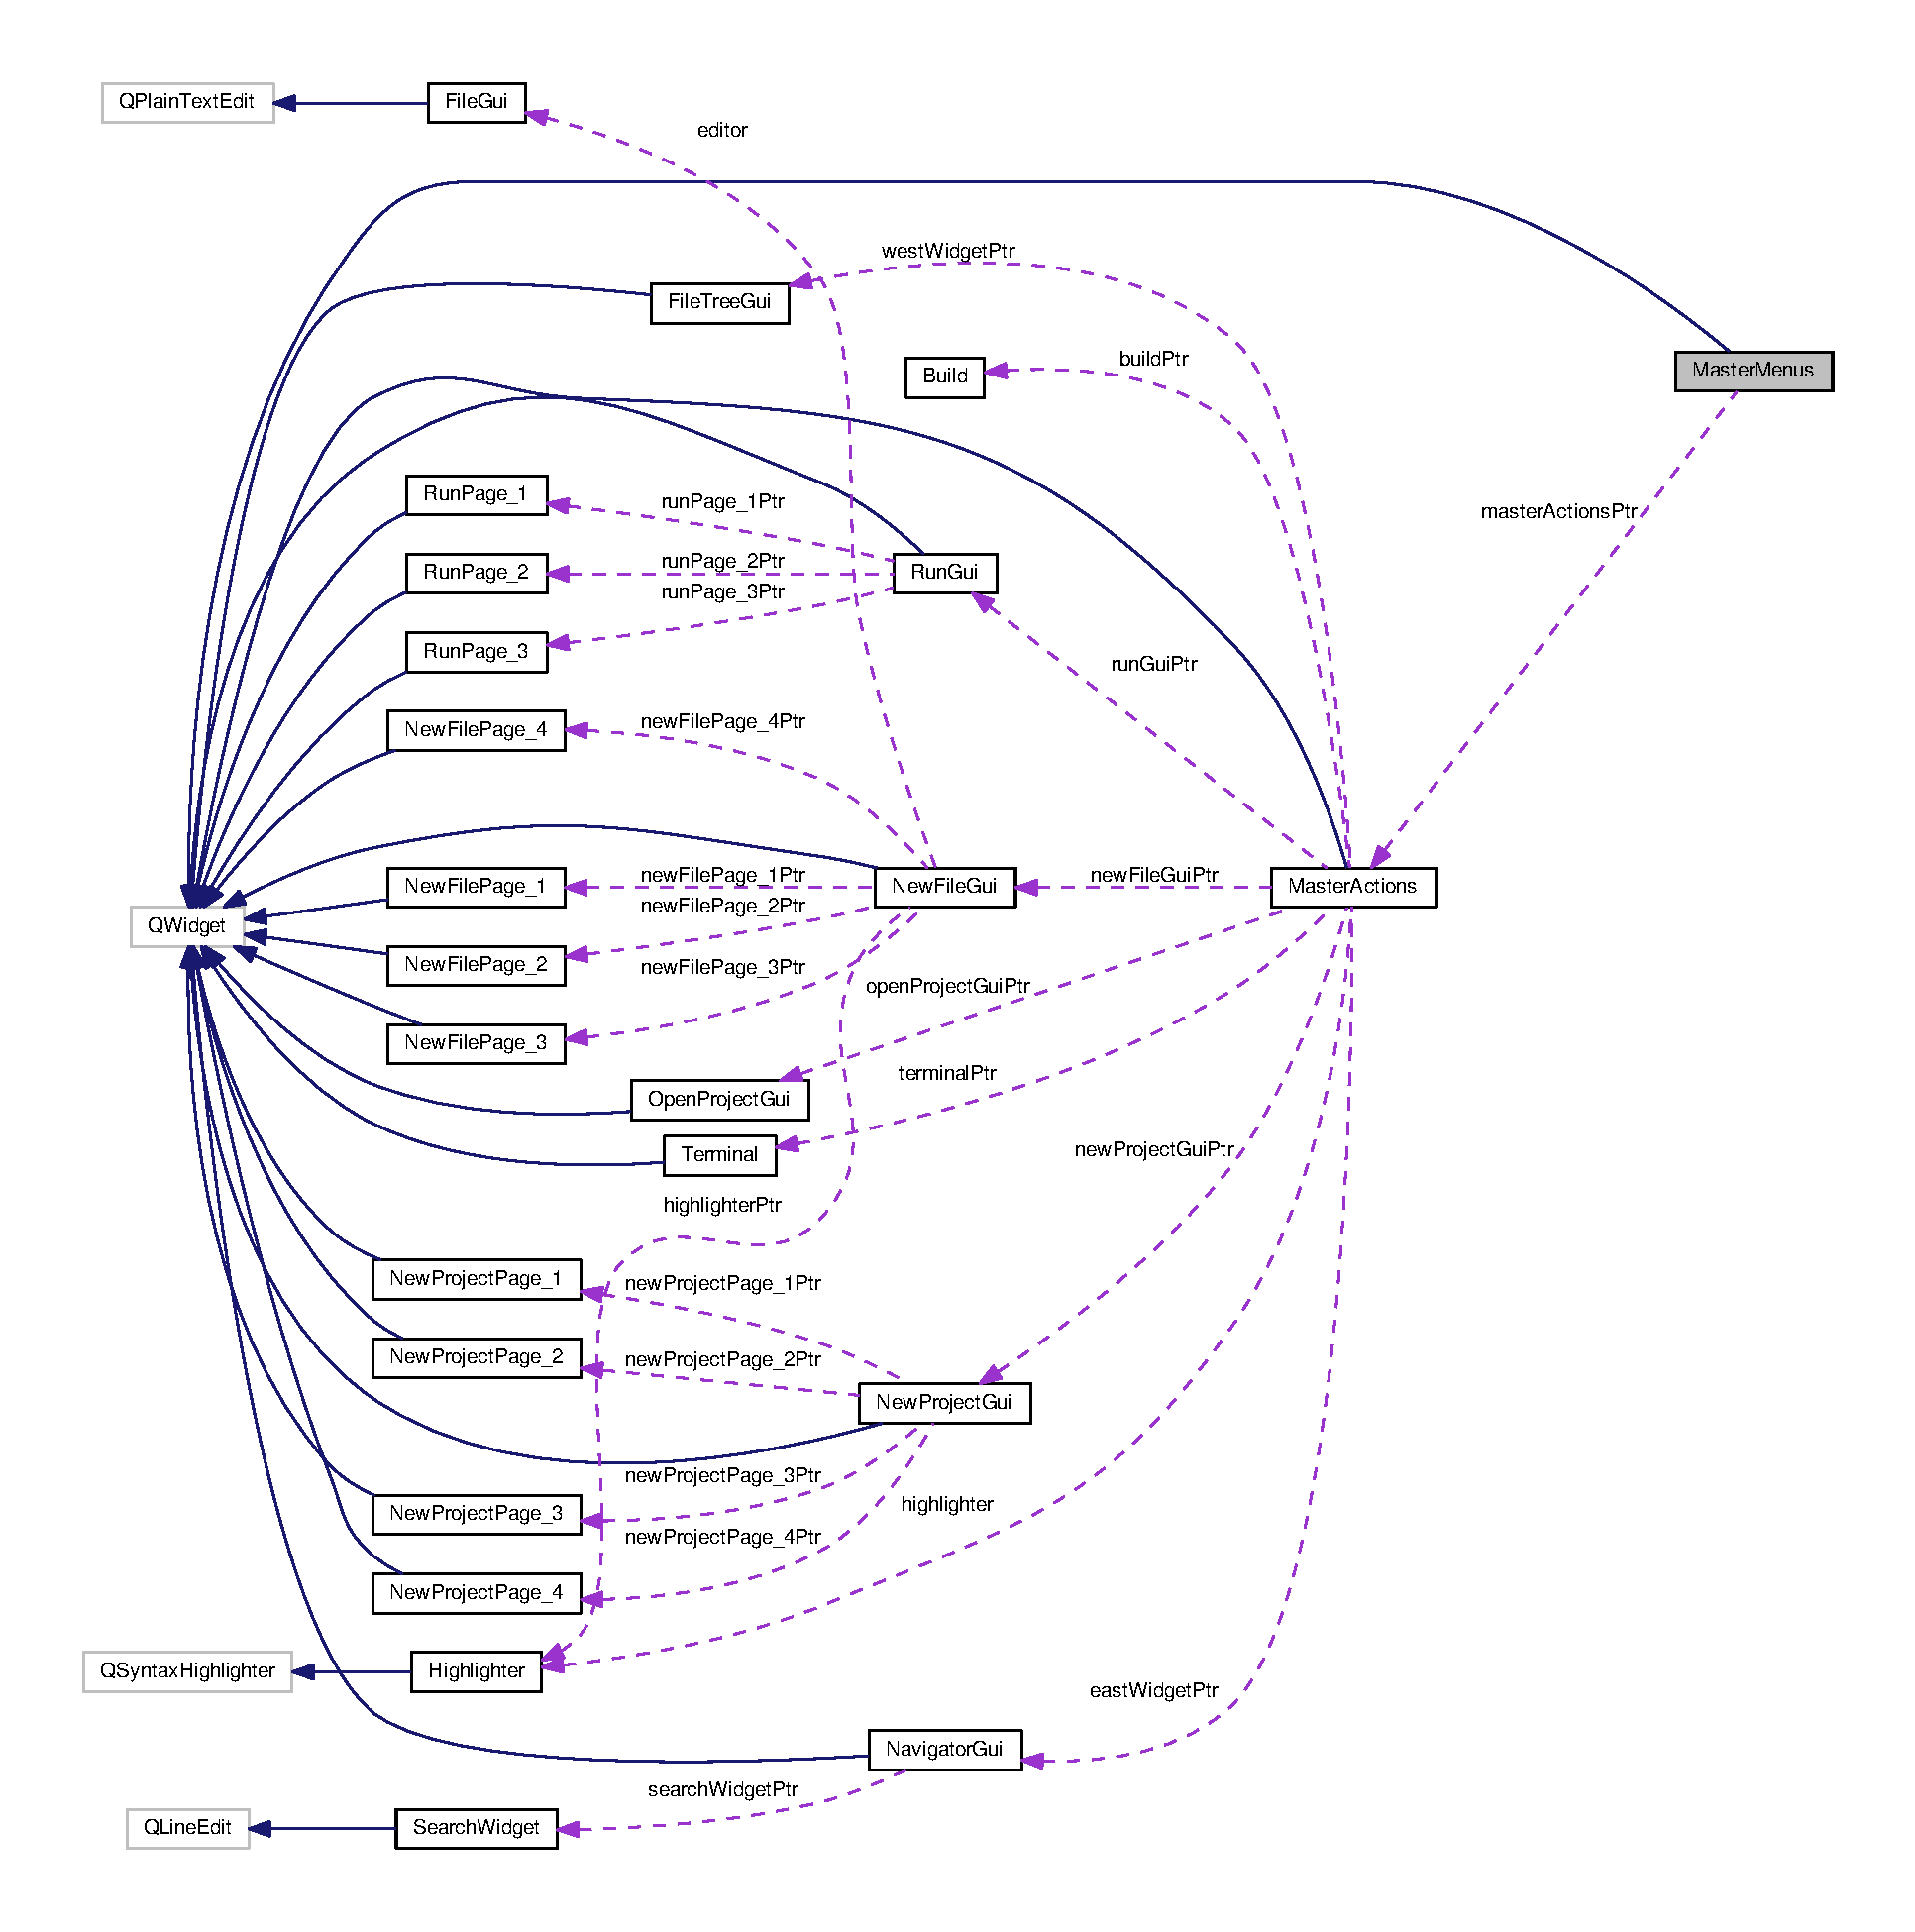
\includegraphics[width=350pt]{class_master_menus__coll__graph}
\end{center}
\end{figure}
\subsection*{Public Member Functions}
\begin{DoxyCompactItemize}
\item 
\hyperlink{class_master_menus_aee36f42f90844440ca2d43dc9b89ba9e}{Master\-Menus} (Q\-Widget $\ast$parent=0)
\item 
void \hyperlink{class_master_menus_a8953d8e2f0cab66bade92acc88fc04a6}{set\-Master\-Actions\-Ptr} (\hyperlink{class_master_actions}{Master\-Actions} $\ast$\hyperlink{class_master_menus_ab5ba9c46b8ad0e6eb11345e055ac469d}{master\-Actions\-Ptr})
\item 
\hyperlink{class_master_actions}{Master\-Actions} $\ast$ \hyperlink{class_master_menus_a391ce8b65f45a7e86461260d3d087d7c}{get\-Master\-Actions\-Ptr} ()
\item 
void \hyperlink{class_master_menus_aa8bc0efcd6904b557923f10135b4a6f0}{init\-File\-Menu\-Ptr} (Q\-Menu $\ast$menu)
\item 
void \hyperlink{class_master_menus_a3e332b9f2c0b1f6f8be1804edc3c3a4a}{init\-Edit\-Menu\-Ptr} (Q\-Menu $\ast$menu)
\item 
void \hyperlink{class_master_menus_a072f53ddc7e95bd21257fa094ee6c143}{init\-View\-Menu\-Ptr} (Q\-Menu $\ast$menu)
\item 
void \hyperlink{class_master_menus_a25403797f3c7541b131e622bf4e204bf}{init\-Navigate\-Menu\-Ptr} (Q\-Menu $\ast$menu)
\item 
void \hyperlink{class_master_menus_a9c2d338a75873eaac4914c7d148c109e}{init\-Source\-Menu\-Ptr} (Q\-Menu $\ast$menu)
\item 
void \hyperlink{class_master_menus_afc4b17087ccac9f443f26b7c881ce2bd}{init\-Refactor\-Menu\-Ptr} (Q\-Menu $\ast$menu)
\item 
void \hyperlink{class_master_menus_a8c9b587f8cfea5f8a49e4200adff5690}{init\-Run\-Menu\-Ptr} (Q\-Menu $\ast$menu)
\item 
void \hyperlink{class_master_menus_a395c8d54738fdb875d87b8f1b4f35285}{init\-Debug\-Menu\-Ptr} (Q\-Menu $\ast$menu)
\item 
void \hyperlink{class_master_menus_a126723492781a9da43f1c50cbfcb3876}{init\-Profile\-Menu\-Ptr} (Q\-Menu $\ast$menu)
\item 
void \hyperlink{class_master_menus_ab30cf69cf56d96abea4a201f6f89afb3}{init\-Team\-Menu\-Ptr} (Q\-Menu $\ast$menu)
\item 
void \hyperlink{class_master_menus_a70590f225ba732935b1b270e01e02270}{init\-Tools\-Menu\-Ptr} (Q\-Menu $\ast$menu)
\item 
void \hyperlink{class_master_menus_a65282d762db712fa3eb44cda48a2a52b}{init\-Window\-Menu\-Ptr} (Q\-Menu $\ast$menu)
\item 
void \hyperlink{class_master_menus_a9351214c416efafee85d1d7930c534f8}{init\-Help\-Menu\-Ptr} (Q\-Menu $\ast$menu)
\item 
\hyperlink{class_master_menus_adce7fedd7b1732fc70ec7fcf3725cf22}{$\sim$\-Master\-Menus} ()
\end{DoxyCompactItemize}
\subsection*{Private Attributes}
\begin{DoxyCompactItemize}
\item 
\hyperlink{class_master_actions}{Master\-Actions} $\ast$ \hyperlink{class_master_menus_ab5ba9c46b8ad0e6eb11345e055ac469d}{master\-Actions\-Ptr}
\end{DoxyCompactItemize}


\subsection{Detailed Description}


Definition at line 21 of file Master\-Menus.\-h.



\subsection{Constructor \& Destructor Documentation}
\hypertarget{class_master_menus_aee36f42f90844440ca2d43dc9b89ba9e}{\index{Master\-Menus@{Master\-Menus}!Master\-Menus@{Master\-Menus}}
\index{Master\-Menus@{Master\-Menus}!MasterMenus@{Master\-Menus}}
\subsubsection[{Master\-Menus}]{\setlength{\rightskip}{0pt plus 5cm}Master\-Menus\-::\-Master\-Menus (
\begin{DoxyParamCaption}
\item[{Q\-Widget $\ast$}]{parent = {\ttfamily 0}}
\end{DoxyParamCaption}
)}}\label{class_master_menus_aee36f42f90844440ca2d43dc9b89ba9e}


Definition at line 4 of file Master\-Menus.\-cpp.

\hypertarget{class_master_menus_adce7fedd7b1732fc70ec7fcf3725cf22}{\index{Master\-Menus@{Master\-Menus}!$\sim$\-Master\-Menus@{$\sim$\-Master\-Menus}}
\index{$\sim$\-Master\-Menus@{$\sim$\-Master\-Menus}!MasterMenus@{Master\-Menus}}
\subsubsection[{$\sim$\-Master\-Menus}]{\setlength{\rightskip}{0pt plus 5cm}Master\-Menus\-::$\sim$\-Master\-Menus (
\begin{DoxyParamCaption}
{}
\end{DoxyParamCaption}
)}}\label{class_master_menus_adce7fedd7b1732fc70ec7fcf3725cf22}


Definition at line 103 of file Master\-Menus.\-cpp.



\subsection{Member Function Documentation}
\hypertarget{class_master_menus_a391ce8b65f45a7e86461260d3d087d7c}{\index{Master\-Menus@{Master\-Menus}!get\-Master\-Actions\-Ptr@{get\-Master\-Actions\-Ptr}}
\index{get\-Master\-Actions\-Ptr@{get\-Master\-Actions\-Ptr}!MasterMenus@{Master\-Menus}}
\subsubsection[{get\-Master\-Actions\-Ptr}]{\setlength{\rightskip}{0pt plus 5cm}{\bf Master\-Actions} $\ast$ Master\-Menus\-::get\-Master\-Actions\-Ptr (
\begin{DoxyParamCaption}
{}
\end{DoxyParamCaption}
)}}\label{class_master_menus_a391ce8b65f45a7e86461260d3d087d7c}


Definition at line 16 of file Master\-Menus.\-cpp.

\hypertarget{class_master_menus_a395c8d54738fdb875d87b8f1b4f35285}{\index{Master\-Menus@{Master\-Menus}!init\-Debug\-Menu\-Ptr@{init\-Debug\-Menu\-Ptr}}
\index{init\-Debug\-Menu\-Ptr@{init\-Debug\-Menu\-Ptr}!MasterMenus@{Master\-Menus}}
\subsubsection[{init\-Debug\-Menu\-Ptr}]{\setlength{\rightskip}{0pt plus 5cm}void Master\-Menus\-::init\-Debug\-Menu\-Ptr (
\begin{DoxyParamCaption}
\item[{Q\-Menu $\ast$}]{menu}
\end{DoxyParamCaption}
)}}\label{class_master_menus_a395c8d54738fdb875d87b8f1b4f35285}


Definition at line 67 of file Master\-Menus.\-cpp.



Here is the caller graph for this function\-:
\nopagebreak
\begin{figure}[H]
\begin{center}
\leavevmode
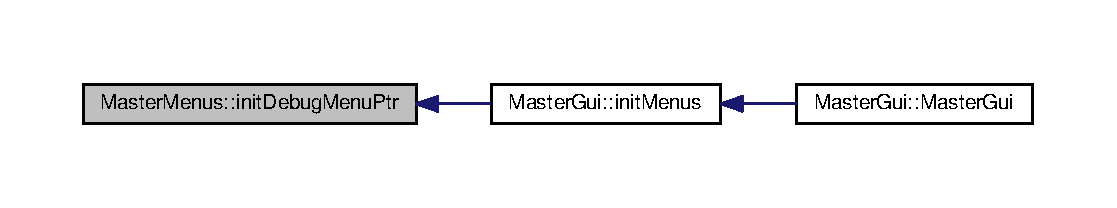
\includegraphics[width=350pt]{class_master_menus_a395c8d54738fdb875d87b8f1b4f35285_icgraph}
\end{center}
\end{figure}


\hypertarget{class_master_menus_a3e332b9f2c0b1f6f8be1804edc3c3a4a}{\index{Master\-Menus@{Master\-Menus}!init\-Edit\-Menu\-Ptr@{init\-Edit\-Menu\-Ptr}}
\index{init\-Edit\-Menu\-Ptr@{init\-Edit\-Menu\-Ptr}!MasterMenus@{Master\-Menus}}
\subsubsection[{init\-Edit\-Menu\-Ptr}]{\setlength{\rightskip}{0pt plus 5cm}void Master\-Menus\-::init\-Edit\-Menu\-Ptr (
\begin{DoxyParamCaption}
\item[{Q\-Menu $\ast$}]{menu}
\end{DoxyParamCaption}
)}}\label{class_master_menus_a3e332b9f2c0b1f6f8be1804edc3c3a4a}


Definition at line 30 of file Master\-Menus.\-cpp.



Here is the call graph for this function\-:
\nopagebreak
\begin{figure}[H]
\begin{center}
\leavevmode
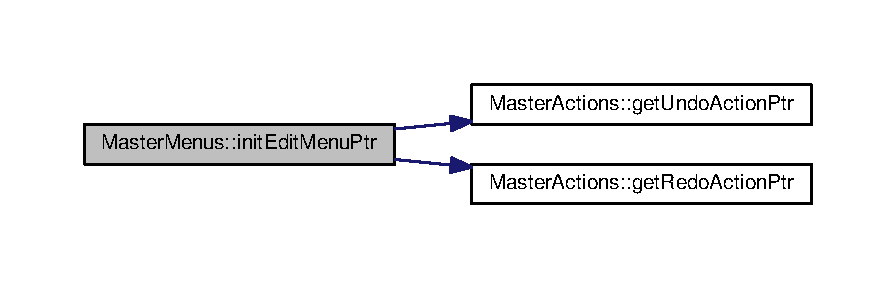
\includegraphics[width=350pt]{class_master_menus_a3e332b9f2c0b1f6f8be1804edc3c3a4a_cgraph}
\end{center}
\end{figure}




Here is the caller graph for this function\-:
\nopagebreak
\begin{figure}[H]
\begin{center}
\leavevmode
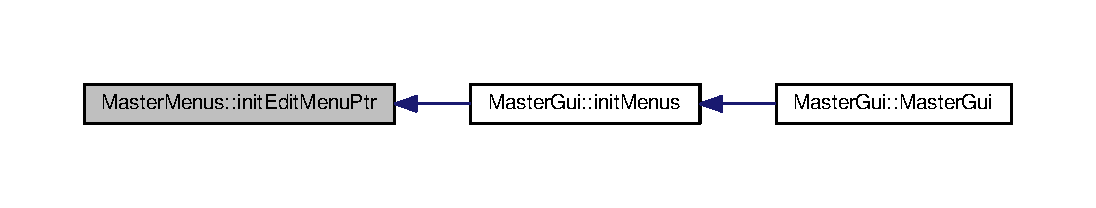
\includegraphics[width=350pt]{class_master_menus_a3e332b9f2c0b1f6f8be1804edc3c3a4a_icgraph}
\end{center}
\end{figure}


\hypertarget{class_master_menus_aa8bc0efcd6904b557923f10135b4a6f0}{\index{Master\-Menus@{Master\-Menus}!init\-File\-Menu\-Ptr@{init\-File\-Menu\-Ptr}}
\index{init\-File\-Menu\-Ptr@{init\-File\-Menu\-Ptr}!MasterMenus@{Master\-Menus}}
\subsubsection[{init\-File\-Menu\-Ptr}]{\setlength{\rightskip}{0pt plus 5cm}void Master\-Menus\-::init\-File\-Menu\-Ptr (
\begin{DoxyParamCaption}
\item[{Q\-Menu $\ast$}]{menu}
\end{DoxyParamCaption}
)}}\label{class_master_menus_aa8bc0efcd6904b557923f10135b4a6f0}


Definition at line 22 of file Master\-Menus.\-cpp.



Here is the call graph for this function\-:
\nopagebreak
\begin{figure}[H]
\begin{center}
\leavevmode
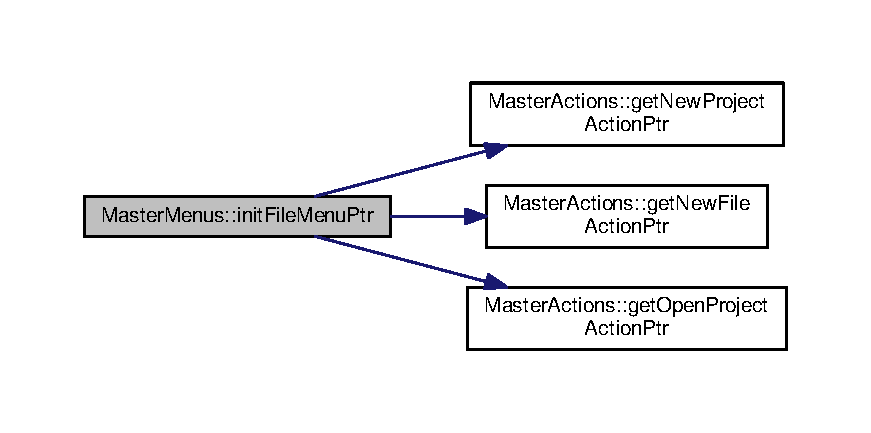
\includegraphics[width=350pt]{class_master_menus_aa8bc0efcd6904b557923f10135b4a6f0_cgraph}
\end{center}
\end{figure}




Here is the caller graph for this function\-:
\nopagebreak
\begin{figure}[H]
\begin{center}
\leavevmode
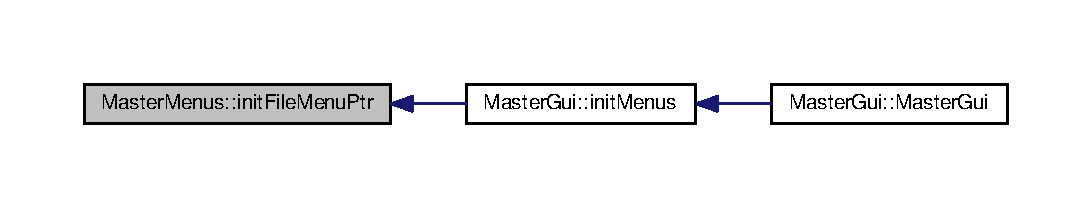
\includegraphics[width=350pt]{class_master_menus_aa8bc0efcd6904b557923f10135b4a6f0_icgraph}
\end{center}
\end{figure}


\hypertarget{class_master_menus_a9351214c416efafee85d1d7930c534f8}{\index{Master\-Menus@{Master\-Menus}!init\-Help\-Menu\-Ptr@{init\-Help\-Menu\-Ptr}}
\index{init\-Help\-Menu\-Ptr@{init\-Help\-Menu\-Ptr}!MasterMenus@{Master\-Menus}}
\subsubsection[{init\-Help\-Menu\-Ptr}]{\setlength{\rightskip}{0pt plus 5cm}void Master\-Menus\-::init\-Help\-Menu\-Ptr (
\begin{DoxyParamCaption}
\item[{Q\-Menu $\ast$}]{menu}
\end{DoxyParamCaption}
)}}\label{class_master_menus_a9351214c416efafee85d1d7930c534f8}


Definition at line 97 of file Master\-Menus.\-cpp.



Here is the caller graph for this function\-:
\nopagebreak
\begin{figure}[H]
\begin{center}
\leavevmode
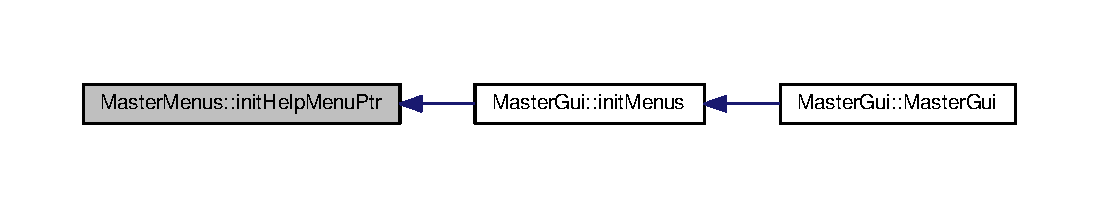
\includegraphics[width=350pt]{class_master_menus_a9351214c416efafee85d1d7930c534f8_icgraph}
\end{center}
\end{figure}


\hypertarget{class_master_menus_a25403797f3c7541b131e622bf4e204bf}{\index{Master\-Menus@{Master\-Menus}!init\-Navigate\-Menu\-Ptr@{init\-Navigate\-Menu\-Ptr}}
\index{init\-Navigate\-Menu\-Ptr@{init\-Navigate\-Menu\-Ptr}!MasterMenus@{Master\-Menus}}
\subsubsection[{init\-Navigate\-Menu\-Ptr}]{\setlength{\rightskip}{0pt plus 5cm}void Master\-Menus\-::init\-Navigate\-Menu\-Ptr (
\begin{DoxyParamCaption}
\item[{Q\-Menu $\ast$}]{menu}
\end{DoxyParamCaption}
)}}\label{class_master_menus_a25403797f3c7541b131e622bf4e204bf}


Definition at line 43 of file Master\-Menus.\-cpp.



Here is the caller graph for this function\-:
\nopagebreak
\begin{figure}[H]
\begin{center}
\leavevmode
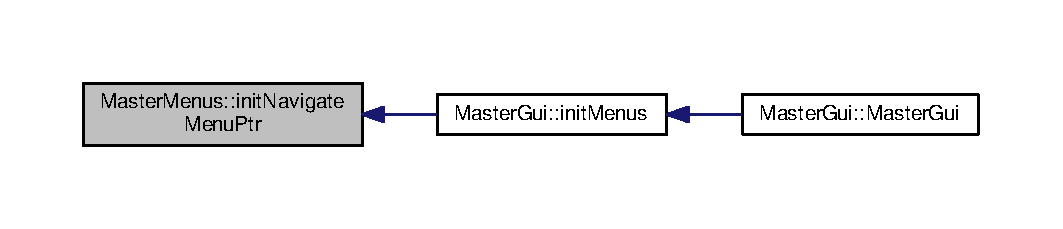
\includegraphics[width=350pt]{class_master_menus_a25403797f3c7541b131e622bf4e204bf_icgraph}
\end{center}
\end{figure}


\hypertarget{class_master_menus_a126723492781a9da43f1c50cbfcb3876}{\index{Master\-Menus@{Master\-Menus}!init\-Profile\-Menu\-Ptr@{init\-Profile\-Menu\-Ptr}}
\index{init\-Profile\-Menu\-Ptr@{init\-Profile\-Menu\-Ptr}!MasterMenus@{Master\-Menus}}
\subsubsection[{init\-Profile\-Menu\-Ptr}]{\setlength{\rightskip}{0pt plus 5cm}void Master\-Menus\-::init\-Profile\-Menu\-Ptr (
\begin{DoxyParamCaption}
\item[{Q\-Menu $\ast$}]{menu}
\end{DoxyParamCaption}
)}}\label{class_master_menus_a126723492781a9da43f1c50cbfcb3876}


Definition at line 73 of file Master\-Menus.\-cpp.



Here is the caller graph for this function\-:
\nopagebreak
\begin{figure}[H]
\begin{center}
\leavevmode
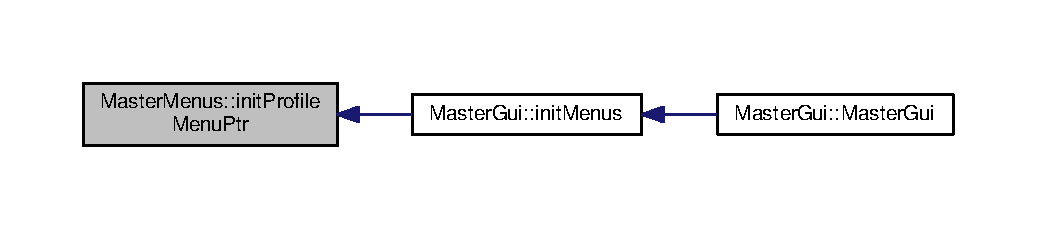
\includegraphics[width=350pt]{class_master_menus_a126723492781a9da43f1c50cbfcb3876_icgraph}
\end{center}
\end{figure}


\hypertarget{class_master_menus_afc4b17087ccac9f443f26b7c881ce2bd}{\index{Master\-Menus@{Master\-Menus}!init\-Refactor\-Menu\-Ptr@{init\-Refactor\-Menu\-Ptr}}
\index{init\-Refactor\-Menu\-Ptr@{init\-Refactor\-Menu\-Ptr}!MasterMenus@{Master\-Menus}}
\subsubsection[{init\-Refactor\-Menu\-Ptr}]{\setlength{\rightskip}{0pt plus 5cm}void Master\-Menus\-::init\-Refactor\-Menu\-Ptr (
\begin{DoxyParamCaption}
\item[{Q\-Menu $\ast$}]{menu}
\end{DoxyParamCaption}
)}}\label{class_master_menus_afc4b17087ccac9f443f26b7c881ce2bd}


Definition at line 55 of file Master\-Menus.\-cpp.



Here is the caller graph for this function\-:
\nopagebreak
\begin{figure}[H]
\begin{center}
\leavevmode
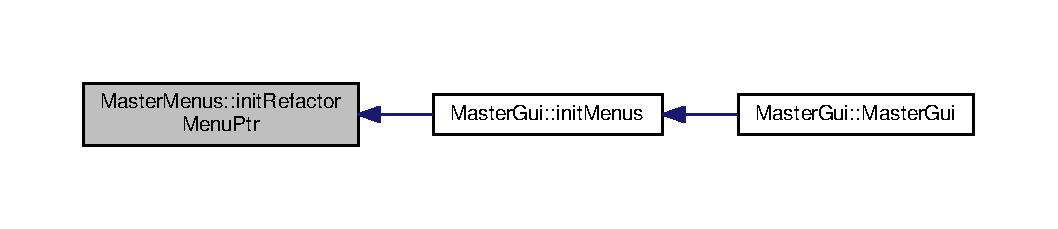
\includegraphics[width=350pt]{class_master_menus_afc4b17087ccac9f443f26b7c881ce2bd_icgraph}
\end{center}
\end{figure}


\hypertarget{class_master_menus_a8c9b587f8cfea5f8a49e4200adff5690}{\index{Master\-Menus@{Master\-Menus}!init\-Run\-Menu\-Ptr@{init\-Run\-Menu\-Ptr}}
\index{init\-Run\-Menu\-Ptr@{init\-Run\-Menu\-Ptr}!MasterMenus@{Master\-Menus}}
\subsubsection[{init\-Run\-Menu\-Ptr}]{\setlength{\rightskip}{0pt plus 5cm}void Master\-Menus\-::init\-Run\-Menu\-Ptr (
\begin{DoxyParamCaption}
\item[{Q\-Menu $\ast$}]{menu}
\end{DoxyParamCaption}
)}}\label{class_master_menus_a8c9b587f8cfea5f8a49e4200adff5690}


Definition at line 61 of file Master\-Menus.\-cpp.



Here is the caller graph for this function\-:
\nopagebreak
\begin{figure}[H]
\begin{center}
\leavevmode
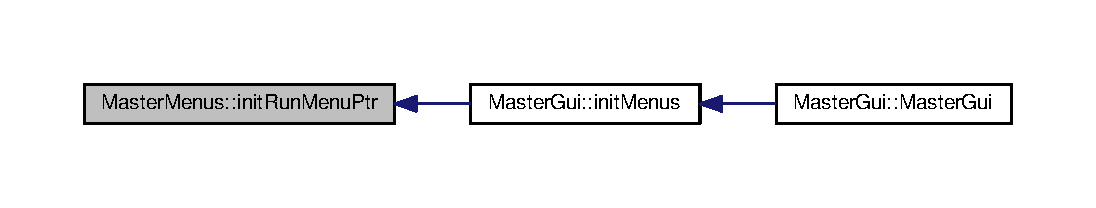
\includegraphics[width=350pt]{class_master_menus_a8c9b587f8cfea5f8a49e4200adff5690_icgraph}
\end{center}
\end{figure}


\hypertarget{class_master_menus_a9c2d338a75873eaac4914c7d148c109e}{\index{Master\-Menus@{Master\-Menus}!init\-Source\-Menu\-Ptr@{init\-Source\-Menu\-Ptr}}
\index{init\-Source\-Menu\-Ptr@{init\-Source\-Menu\-Ptr}!MasterMenus@{Master\-Menus}}
\subsubsection[{init\-Source\-Menu\-Ptr}]{\setlength{\rightskip}{0pt plus 5cm}void Master\-Menus\-::init\-Source\-Menu\-Ptr (
\begin{DoxyParamCaption}
\item[{Q\-Menu $\ast$}]{menu}
\end{DoxyParamCaption}
)}}\label{class_master_menus_a9c2d338a75873eaac4914c7d148c109e}


Definition at line 49 of file Master\-Menus.\-cpp.



Here is the caller graph for this function\-:
\nopagebreak
\begin{figure}[H]
\begin{center}
\leavevmode
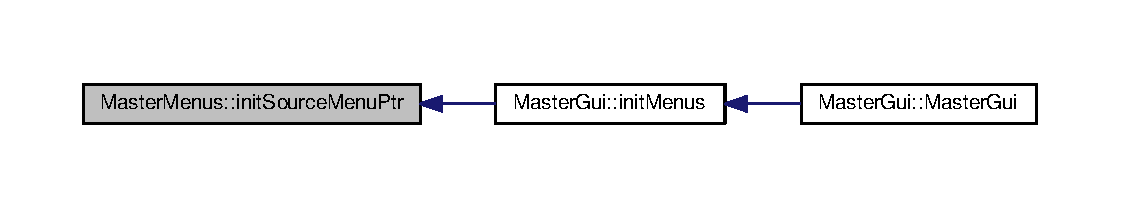
\includegraphics[width=350pt]{class_master_menus_a9c2d338a75873eaac4914c7d148c109e_icgraph}
\end{center}
\end{figure}


\hypertarget{class_master_menus_ab30cf69cf56d96abea4a201f6f89afb3}{\index{Master\-Menus@{Master\-Menus}!init\-Team\-Menu\-Ptr@{init\-Team\-Menu\-Ptr}}
\index{init\-Team\-Menu\-Ptr@{init\-Team\-Menu\-Ptr}!MasterMenus@{Master\-Menus}}
\subsubsection[{init\-Team\-Menu\-Ptr}]{\setlength{\rightskip}{0pt plus 5cm}void Master\-Menus\-::init\-Team\-Menu\-Ptr (
\begin{DoxyParamCaption}
\item[{Q\-Menu $\ast$}]{menu}
\end{DoxyParamCaption}
)}}\label{class_master_menus_ab30cf69cf56d96abea4a201f6f89afb3}


Definition at line 79 of file Master\-Menus.\-cpp.



Here is the caller graph for this function\-:
\nopagebreak
\begin{figure}[H]
\begin{center}
\leavevmode
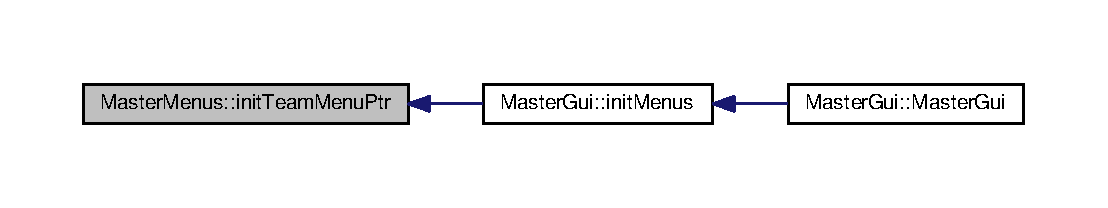
\includegraphics[width=350pt]{class_master_menus_ab30cf69cf56d96abea4a201f6f89afb3_icgraph}
\end{center}
\end{figure}


\hypertarget{class_master_menus_a70590f225ba732935b1b270e01e02270}{\index{Master\-Menus@{Master\-Menus}!init\-Tools\-Menu\-Ptr@{init\-Tools\-Menu\-Ptr}}
\index{init\-Tools\-Menu\-Ptr@{init\-Tools\-Menu\-Ptr}!MasterMenus@{Master\-Menus}}
\subsubsection[{init\-Tools\-Menu\-Ptr}]{\setlength{\rightskip}{0pt plus 5cm}void Master\-Menus\-::init\-Tools\-Menu\-Ptr (
\begin{DoxyParamCaption}
\item[{Q\-Menu $\ast$}]{menu}
\end{DoxyParamCaption}
)}}\label{class_master_menus_a70590f225ba732935b1b270e01e02270}


Definition at line 85 of file Master\-Menus.\-cpp.



Here is the caller graph for this function\-:
\nopagebreak
\begin{figure}[H]
\begin{center}
\leavevmode
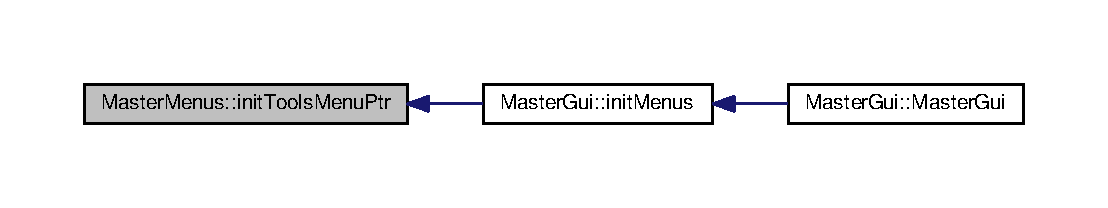
\includegraphics[width=350pt]{class_master_menus_a70590f225ba732935b1b270e01e02270_icgraph}
\end{center}
\end{figure}


\hypertarget{class_master_menus_a072f53ddc7e95bd21257fa094ee6c143}{\index{Master\-Menus@{Master\-Menus}!init\-View\-Menu\-Ptr@{init\-View\-Menu\-Ptr}}
\index{init\-View\-Menu\-Ptr@{init\-View\-Menu\-Ptr}!MasterMenus@{Master\-Menus}}
\subsubsection[{init\-View\-Menu\-Ptr}]{\setlength{\rightskip}{0pt plus 5cm}void Master\-Menus\-::init\-View\-Menu\-Ptr (
\begin{DoxyParamCaption}
\item[{Q\-Menu $\ast$}]{menu}
\end{DoxyParamCaption}
)}}\label{class_master_menus_a072f53ddc7e95bd21257fa094ee6c143}


Definition at line 37 of file Master\-Menus.\-cpp.



Here is the caller graph for this function\-:
\nopagebreak
\begin{figure}[H]
\begin{center}
\leavevmode
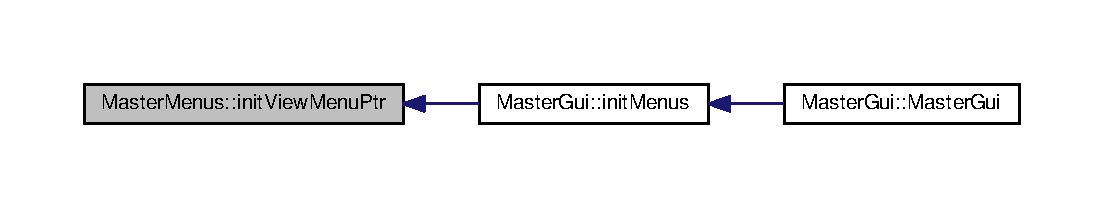
\includegraphics[width=350pt]{class_master_menus_a072f53ddc7e95bd21257fa094ee6c143_icgraph}
\end{center}
\end{figure}


\hypertarget{class_master_menus_a65282d762db712fa3eb44cda48a2a52b}{\index{Master\-Menus@{Master\-Menus}!init\-Window\-Menu\-Ptr@{init\-Window\-Menu\-Ptr}}
\index{init\-Window\-Menu\-Ptr@{init\-Window\-Menu\-Ptr}!MasterMenus@{Master\-Menus}}
\subsubsection[{init\-Window\-Menu\-Ptr}]{\setlength{\rightskip}{0pt plus 5cm}void Master\-Menus\-::init\-Window\-Menu\-Ptr (
\begin{DoxyParamCaption}
\item[{Q\-Menu $\ast$}]{menu}
\end{DoxyParamCaption}
)}}\label{class_master_menus_a65282d762db712fa3eb44cda48a2a52b}


Definition at line 91 of file Master\-Menus.\-cpp.



Here is the caller graph for this function\-:
\nopagebreak
\begin{figure}[H]
\begin{center}
\leavevmode
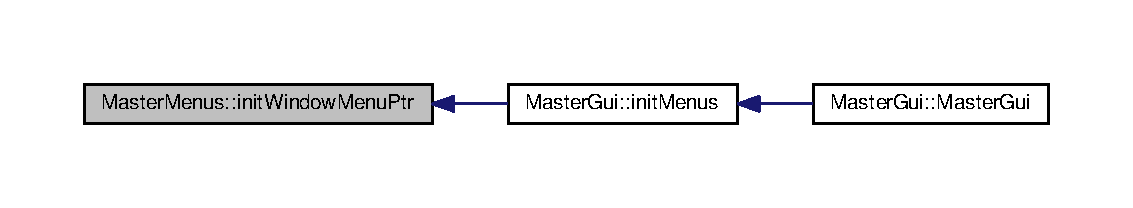
\includegraphics[width=350pt]{class_master_menus_a65282d762db712fa3eb44cda48a2a52b_icgraph}
\end{center}
\end{figure}


\hypertarget{class_master_menus_a8953d8e2f0cab66bade92acc88fc04a6}{\index{Master\-Menus@{Master\-Menus}!set\-Master\-Actions\-Ptr@{set\-Master\-Actions\-Ptr}}
\index{set\-Master\-Actions\-Ptr@{set\-Master\-Actions\-Ptr}!MasterMenus@{Master\-Menus}}
\subsubsection[{set\-Master\-Actions\-Ptr}]{\setlength{\rightskip}{0pt plus 5cm}void Master\-Menus\-::set\-Master\-Actions\-Ptr (
\begin{DoxyParamCaption}
\item[{{\bf Master\-Actions} $\ast$}]{master\-Actions\-Ptr}
\end{DoxyParamCaption}
)}}\label{class_master_menus_a8953d8e2f0cab66bade92acc88fc04a6}


Definition at line 10 of file Master\-Menus.\-cpp.



Here is the caller graph for this function\-:
\nopagebreak
\begin{figure}[H]
\begin{center}
\leavevmode
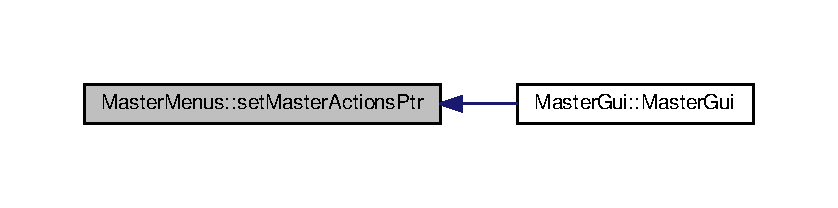
\includegraphics[width=350pt]{class_master_menus_a8953d8e2f0cab66bade92acc88fc04a6_icgraph}
\end{center}
\end{figure}




\subsection{Member Data Documentation}
\hypertarget{class_master_menus_ab5ba9c46b8ad0e6eb11345e055ac469d}{\index{Master\-Menus@{Master\-Menus}!master\-Actions\-Ptr@{master\-Actions\-Ptr}}
\index{master\-Actions\-Ptr@{master\-Actions\-Ptr}!MasterMenus@{Master\-Menus}}
\subsubsection[{master\-Actions\-Ptr}]{\setlength{\rightskip}{0pt plus 5cm}{\bf Master\-Actions}$\ast$ Master\-Menus\-::master\-Actions\-Ptr\hspace{0.3cm}{\ttfamily [private]}}}\label{class_master_menus_ab5ba9c46b8ad0e6eb11345e055ac469d}


Definition at line 26 of file Master\-Menus.\-h.



The documentation for this class was generated from the following files\-:\begin{DoxyCompactItemize}
\item 
/home/james/\-Net\-Beans\-Projects/ride/src/\hyperlink{_master_menus_8h}{Master\-Menus.\-h}\item 
/home/james/\-Net\-Beans\-Projects/ride/src/\hyperlink{_master_menus_8cpp}{Master\-Menus.\-cpp}\end{DoxyCompactItemize}

\hypertarget{class_master_status_bar}{\section{Master\-Status\-Bar Class Reference}
\label{class_master_status_bar}\index{Master\-Status\-Bar@{Master\-Status\-Bar}}
}


{\ttfamily \#include $<$Master\-Status\-Bar.\-h$>$}



Inheritance diagram for Master\-Status\-Bar\-:\nopagebreak
\begin{figure}[H]
\begin{center}
\leavevmode
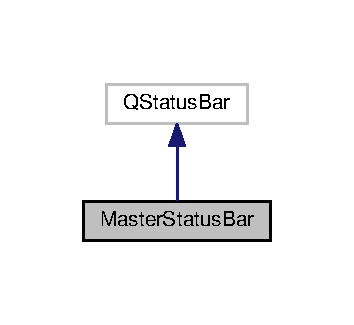
\includegraphics[width=170pt]{class_master_status_bar__inherit__graph}
\end{center}
\end{figure}


Collaboration diagram for Master\-Status\-Bar\-:\nopagebreak
\begin{figure}[H]
\begin{center}
\leavevmode
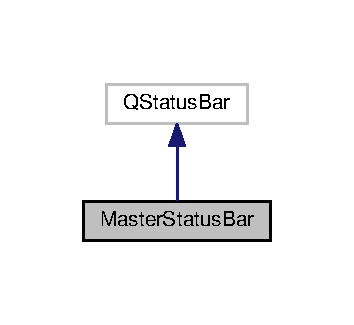
\includegraphics[width=170pt]{class_master_status_bar__coll__graph}
\end{center}
\end{figure}
\subsection*{Public Member Functions}
\begin{DoxyCompactItemize}
\item 
\hyperlink{class_master_status_bar_a773f6af002aeed9a3896bc89498ef66c}{Master\-Status\-Bar} ()
\item 
void \hyperlink{class_master_status_bar_aa5b964babad852afccb8654c4386cb31}{init\-Progress\-Bar\-Ptr} ()
\item 
\hyperlink{class_master_status_bar_ab6c1c48a1481006d73cf1c0de2eb4047}{$\sim$\-Master\-Status\-Bar} ()
\end{DoxyCompactItemize}
\subsection*{Private Attributes}
\begin{DoxyCompactItemize}
\item 
Q\-Progress\-Bar $\ast$ \hyperlink{class_master_status_bar_a4f1c75f98f848f39b92c6ebba539fdae}{progress\-Bar\-Ptr}
\end{DoxyCompactItemize}


\subsection{Detailed Description}


Definition at line 18 of file Master\-Status\-Bar.\-h.



\subsection{Constructor \& Destructor Documentation}
\hypertarget{class_master_status_bar_a773f6af002aeed9a3896bc89498ef66c}{\index{Master\-Status\-Bar@{Master\-Status\-Bar}!Master\-Status\-Bar@{Master\-Status\-Bar}}
\index{Master\-Status\-Bar@{Master\-Status\-Bar}!MasterStatusBar@{Master\-Status\-Bar}}
\subsubsection[{Master\-Status\-Bar}]{\setlength{\rightskip}{0pt plus 5cm}Master\-Status\-Bar\-::\-Master\-Status\-Bar (
\begin{DoxyParamCaption}
{}
\end{DoxyParamCaption}
)}}\label{class_master_status_bar_a773f6af002aeed9a3896bc89498ef66c}


Definition at line 4 of file Master\-Status\-Bar.\-cpp.

\hypertarget{class_master_status_bar_ab6c1c48a1481006d73cf1c0de2eb4047}{\index{Master\-Status\-Bar@{Master\-Status\-Bar}!$\sim$\-Master\-Status\-Bar@{$\sim$\-Master\-Status\-Bar}}
\index{$\sim$\-Master\-Status\-Bar@{$\sim$\-Master\-Status\-Bar}!MasterStatusBar@{Master\-Status\-Bar}}
\subsubsection[{$\sim$\-Master\-Status\-Bar}]{\setlength{\rightskip}{0pt plus 5cm}Master\-Status\-Bar\-::$\sim$\-Master\-Status\-Bar (
\begin{DoxyParamCaption}
{}
\end{DoxyParamCaption}
)}}\label{class_master_status_bar_ab6c1c48a1481006d73cf1c0de2eb4047}


Definition at line 18 of file Master\-Status\-Bar.\-cpp.



\subsection{Member Function Documentation}
\hypertarget{class_master_status_bar_aa5b964babad852afccb8654c4386cb31}{\index{Master\-Status\-Bar@{Master\-Status\-Bar}!init\-Progress\-Bar\-Ptr@{init\-Progress\-Bar\-Ptr}}
\index{init\-Progress\-Bar\-Ptr@{init\-Progress\-Bar\-Ptr}!MasterStatusBar@{Master\-Status\-Bar}}
\subsubsection[{init\-Progress\-Bar\-Ptr}]{\setlength{\rightskip}{0pt plus 5cm}void Master\-Status\-Bar\-::init\-Progress\-Bar\-Ptr (
\begin{DoxyParamCaption}
{}
\end{DoxyParamCaption}
)}}\label{class_master_status_bar_aa5b964babad852afccb8654c4386cb31}


Definition at line 10 of file Master\-Status\-Bar.\-cpp.



\subsection{Member Data Documentation}
\hypertarget{class_master_status_bar_a4f1c75f98f848f39b92c6ebba539fdae}{\index{Master\-Status\-Bar@{Master\-Status\-Bar}!progress\-Bar\-Ptr@{progress\-Bar\-Ptr}}
\index{progress\-Bar\-Ptr@{progress\-Bar\-Ptr}!MasterStatusBar@{Master\-Status\-Bar}}
\subsubsection[{progress\-Bar\-Ptr}]{\setlength{\rightskip}{0pt plus 5cm}Q\-Progress\-Bar$\ast$ Master\-Status\-Bar\-::progress\-Bar\-Ptr\hspace{0.3cm}{\ttfamily [private]}}}\label{class_master_status_bar_a4f1c75f98f848f39b92c6ebba539fdae}


Definition at line 21 of file Master\-Status\-Bar.\-h.



The documentation for this class was generated from the following files\-:\begin{DoxyCompactItemize}
\item 
/home/james/\-Net\-Beans\-Projects/ride/src/\hyperlink{_master_status_bar_8h}{Master\-Status\-Bar.\-h}\item 
/home/james/\-Net\-Beans\-Projects/ride/src/\hyperlink{_master_status_bar_8cpp}{Master\-Status\-Bar.\-cpp}\end{DoxyCompactItemize}

\hypertarget{class_master_tool_bars}{\section{Master\-Tool\-Bars Class Reference}
\label{class_master_tool_bars}\index{Master\-Tool\-Bars@{Master\-Tool\-Bars}}
}


{\ttfamily \#include $<$Master\-Tool\-Bars.\-h$>$}



Inheritance diagram for Master\-Tool\-Bars\-:\nopagebreak
\begin{figure}[H]
\begin{center}
\leavevmode
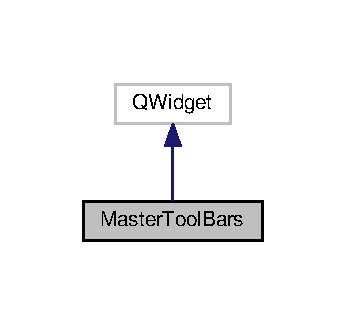
\includegraphics[width=166pt]{class_master_tool_bars__inherit__graph}
\end{center}
\end{figure}


Collaboration diagram for Master\-Tool\-Bars\-:
\nopagebreak
\begin{figure}[H]
\begin{center}
\leavevmode
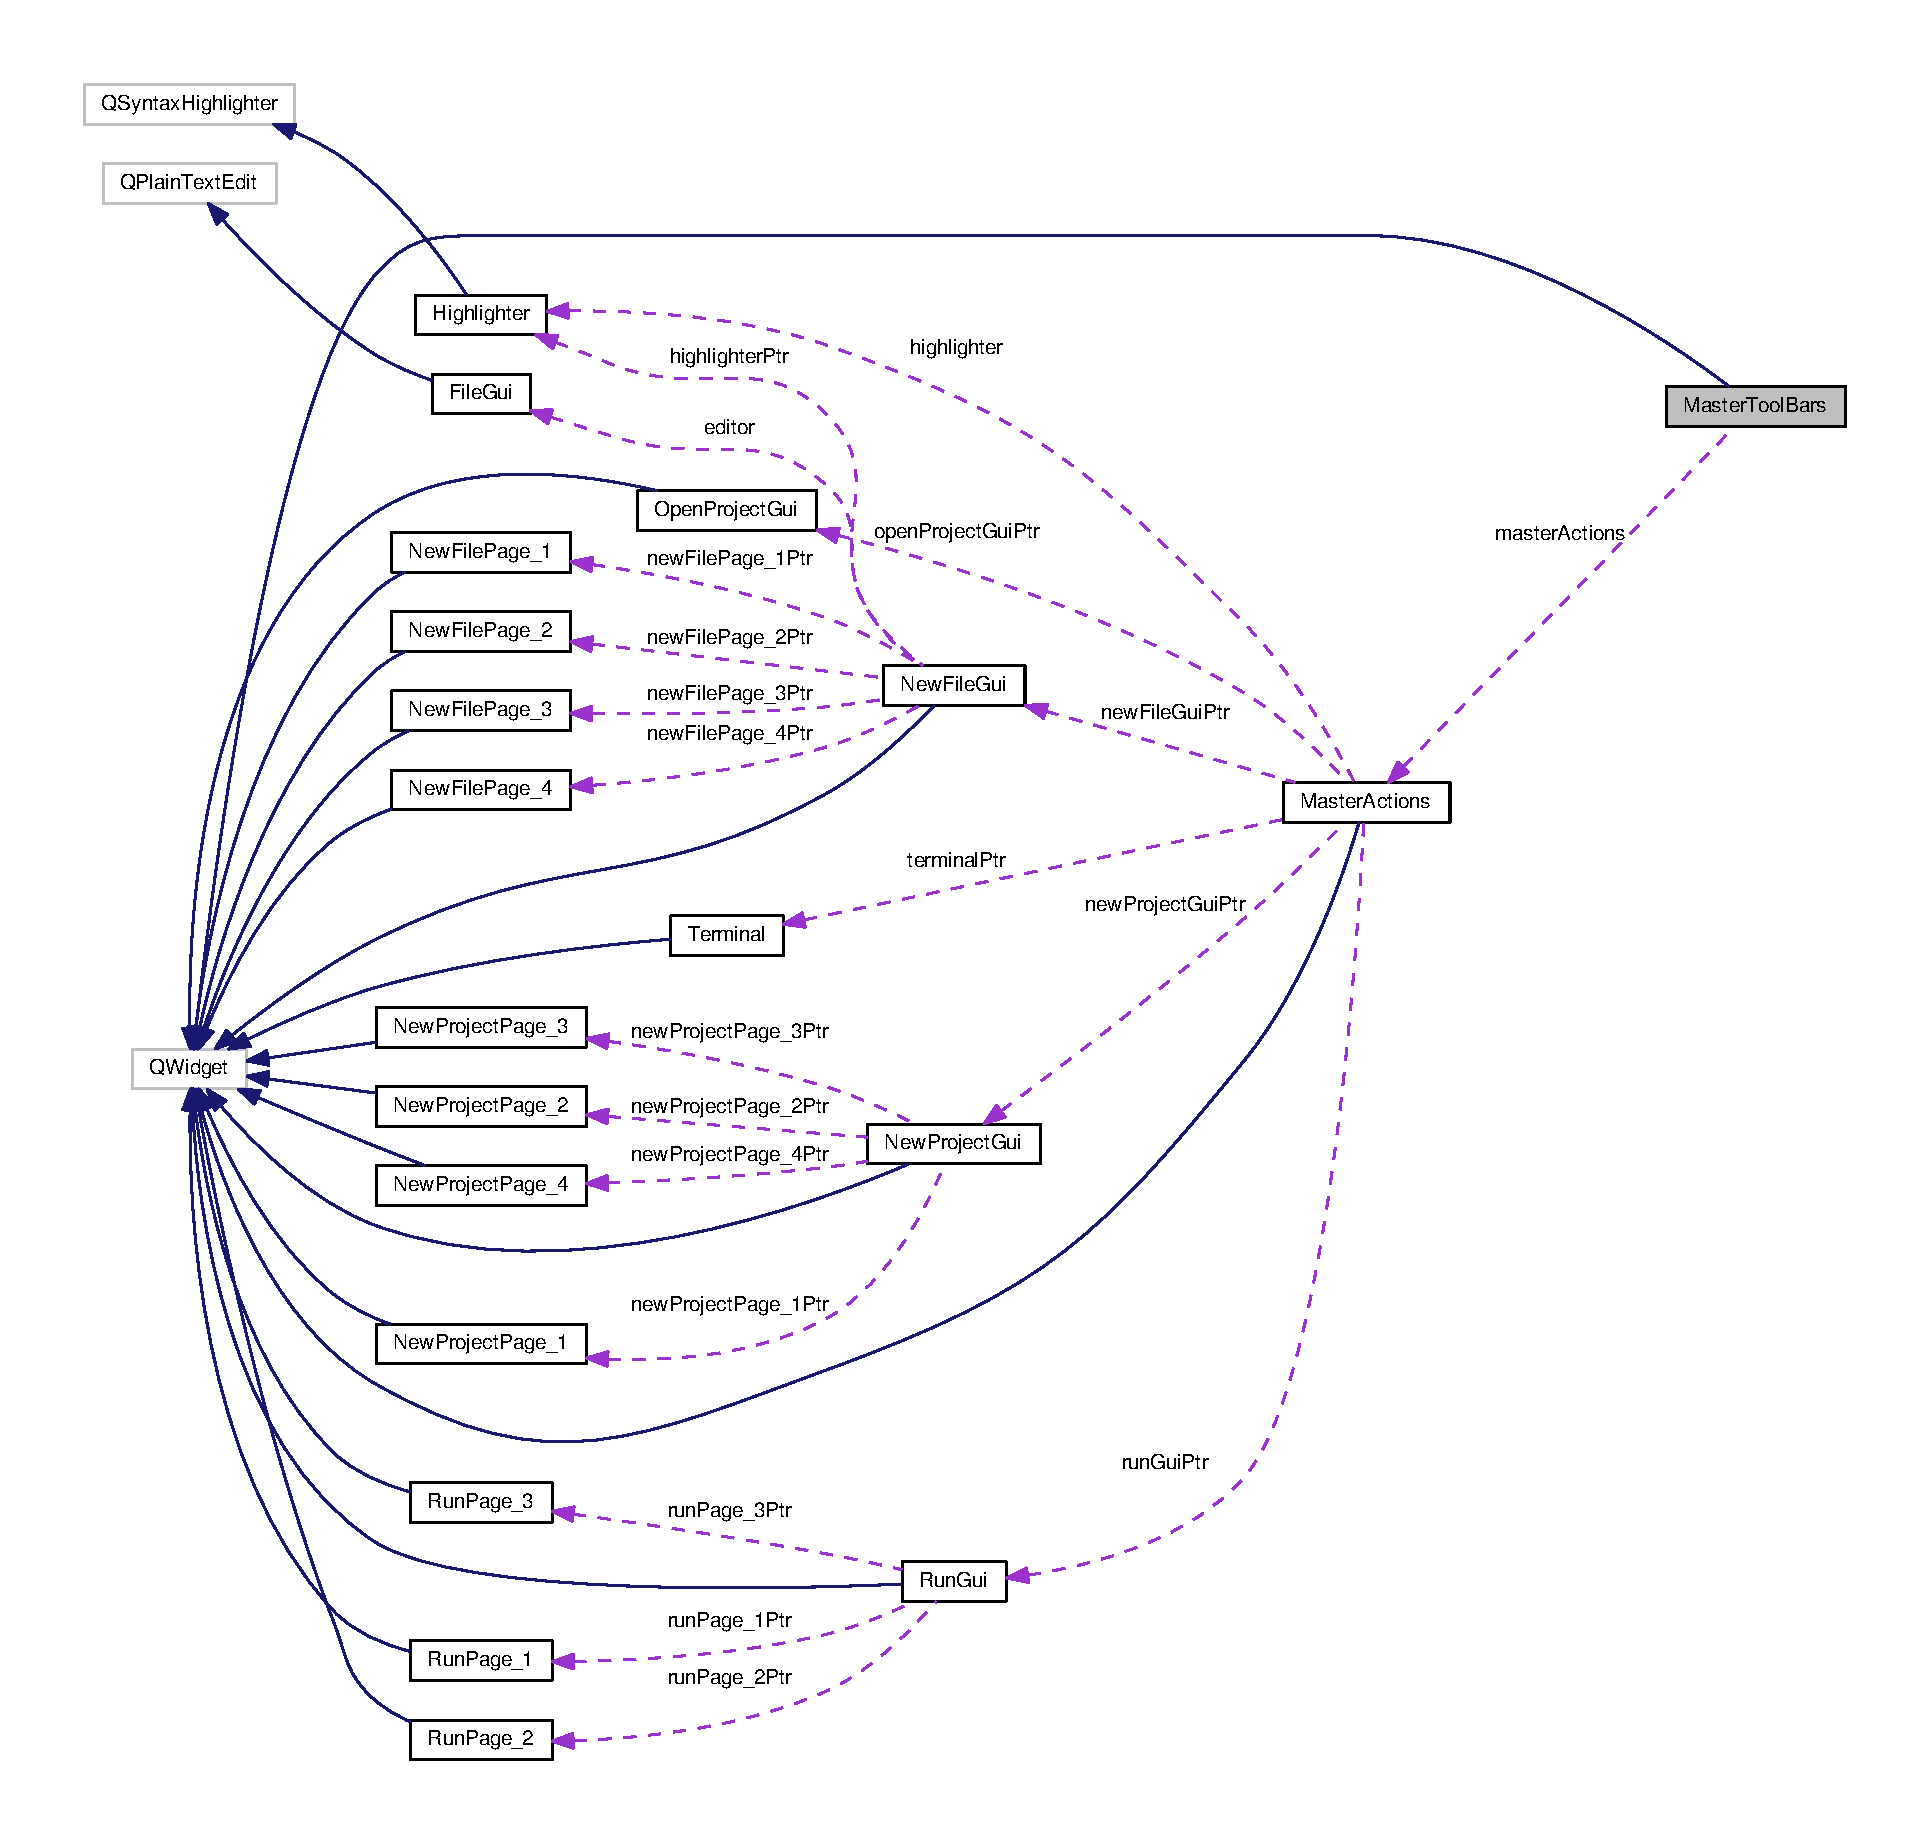
\includegraphics[width=350pt]{class_master_tool_bars__coll__graph}
\end{center}
\end{figure}
\subsection*{Public Member Functions}
\begin{DoxyCompactItemize}
\item 
\hyperlink{class_master_tool_bars_a7f863d99c275bf1efe259281eb3245b0}{Master\-Tool\-Bars} (Q\-Widget $\ast$parent=0)
\item 
void \hyperlink{class_master_tool_bars_a8cc2c4f46779f429221b1dee8ad58181}{set\-Master\-Actions\-Ptr} (\hyperlink{class_master_actions}{Master\-Actions} $\ast$master\-Actions\-Ptr)
\item 
\hyperlink{class_master_actions}{Master\-Actions} $\ast$ \hyperlink{class_master_tool_bars_ae73d5e7f4b317e7402ed0b7f6e405fb9}{get\-Master\-Actions\-Ptr} ()
\item 
void \hyperlink{class_master_tool_bars_aec0df27e89d0bbcf5c7b5fc7d2fa8195}{init\-North\-Group\-One\-Tool\-Bar} (Q\-Tool\-Bar $\ast$toolbar\-Ptr)
\item 
void \hyperlink{class_master_tool_bars_a6b77ec9af9c57217657689b6564f1a54}{init\-North\-Group\-Two\-Tool\-Bar} (Q\-Tool\-Bar $\ast$toolbar\-Ptr)
\item 
void \hyperlink{class_master_tool_bars_a058d8e043fc2d5303e21f993c48bc581}{init\-North\-Group\-Three\-Tool\-Bar} (Q\-Tool\-Bar $\ast$toolbar\-Ptr)
\item 
void \hyperlink{class_master_tool_bars_a3f8d953232c3c8ad2205913514a7233e}{init\-South\-Group\-One\-Tool\-Bar} (Q\-Tool\-Bar $\ast$toolbar\-Ptr)
\item 
void \hyperlink{class_master_tool_bars_ad17aa8fcdbbbc16c67075b5b06db146e}{init\-East\-Group\-One\-Tool\-Bar} (Q\-Tool\-Bar $\ast$toolbar\-Ptr)
\item 
void \hyperlink{class_master_tool_bars_a12bb3e3171d9ea6a6c9cd9c7b800e0d7}{init\-West\-Group\-One\-Tool\-Bar} (Q\-Tool\-Bar $\ast$toolbar\-Ptr)
\item 
\hyperlink{class_master_tool_bars_abde16b63edfa107a7125dee5f9c435be}{$\sim$\-Master\-Tool\-Bars} ()
\end{DoxyCompactItemize}
\subsection*{Private Attributes}
\begin{DoxyCompactItemize}
\item 
\hyperlink{class_master_actions}{Master\-Actions} $\ast$ \hyperlink{class_master_tool_bars_a1adde6a67eaa64fbbbf65ffcb8c1590f}{master\-Actions}
\end{DoxyCompactItemize}


\subsection{Detailed Description}


Definition at line 24 of file Master\-Tool\-Bars.\-h.



\subsection{Constructor \& Destructor Documentation}
\hypertarget{class_master_tool_bars_a7f863d99c275bf1efe259281eb3245b0}{\index{Master\-Tool\-Bars@{Master\-Tool\-Bars}!Master\-Tool\-Bars@{Master\-Tool\-Bars}}
\index{Master\-Tool\-Bars@{Master\-Tool\-Bars}!MasterToolBars@{Master\-Tool\-Bars}}
\subsubsection[{Master\-Tool\-Bars}]{\setlength{\rightskip}{0pt plus 5cm}Master\-Tool\-Bars\-::\-Master\-Tool\-Bars (
\begin{DoxyParamCaption}
\item[{Q\-Widget $\ast$}]{parent = {\ttfamily 0}}
\end{DoxyParamCaption}
)}}\label{class_master_tool_bars_a7f863d99c275bf1efe259281eb3245b0}


Definition at line 4 of file Master\-Tool\-Bars.\-cpp.

\hypertarget{class_master_tool_bars_abde16b63edfa107a7125dee5f9c435be}{\index{Master\-Tool\-Bars@{Master\-Tool\-Bars}!$\sim$\-Master\-Tool\-Bars@{$\sim$\-Master\-Tool\-Bars}}
\index{$\sim$\-Master\-Tool\-Bars@{$\sim$\-Master\-Tool\-Bars}!MasterToolBars@{Master\-Tool\-Bars}}
\subsubsection[{$\sim$\-Master\-Tool\-Bars}]{\setlength{\rightskip}{0pt plus 5cm}Master\-Tool\-Bars\-::$\sim$\-Master\-Tool\-Bars (
\begin{DoxyParamCaption}
{}
\end{DoxyParamCaption}
)}}\label{class_master_tool_bars_abde16b63edfa107a7125dee5f9c435be}


Definition at line 70 of file Master\-Tool\-Bars.\-cpp.



\subsection{Member Function Documentation}
\hypertarget{class_master_tool_bars_ae73d5e7f4b317e7402ed0b7f6e405fb9}{\index{Master\-Tool\-Bars@{Master\-Tool\-Bars}!get\-Master\-Actions\-Ptr@{get\-Master\-Actions\-Ptr}}
\index{get\-Master\-Actions\-Ptr@{get\-Master\-Actions\-Ptr}!MasterToolBars@{Master\-Tool\-Bars}}
\subsubsection[{get\-Master\-Actions\-Ptr}]{\setlength{\rightskip}{0pt plus 5cm}{\bf Master\-Actions} $\ast$ Master\-Tool\-Bars\-::get\-Master\-Actions\-Ptr (
\begin{DoxyParamCaption}
{}
\end{DoxyParamCaption}
)}}\label{class_master_tool_bars_ae73d5e7f4b317e7402ed0b7f6e405fb9}


Definition at line 15 of file Master\-Tool\-Bars.\-cpp.



Here is the caller graph for this function\-:
\nopagebreak
\begin{figure}[H]
\begin{center}
\leavevmode
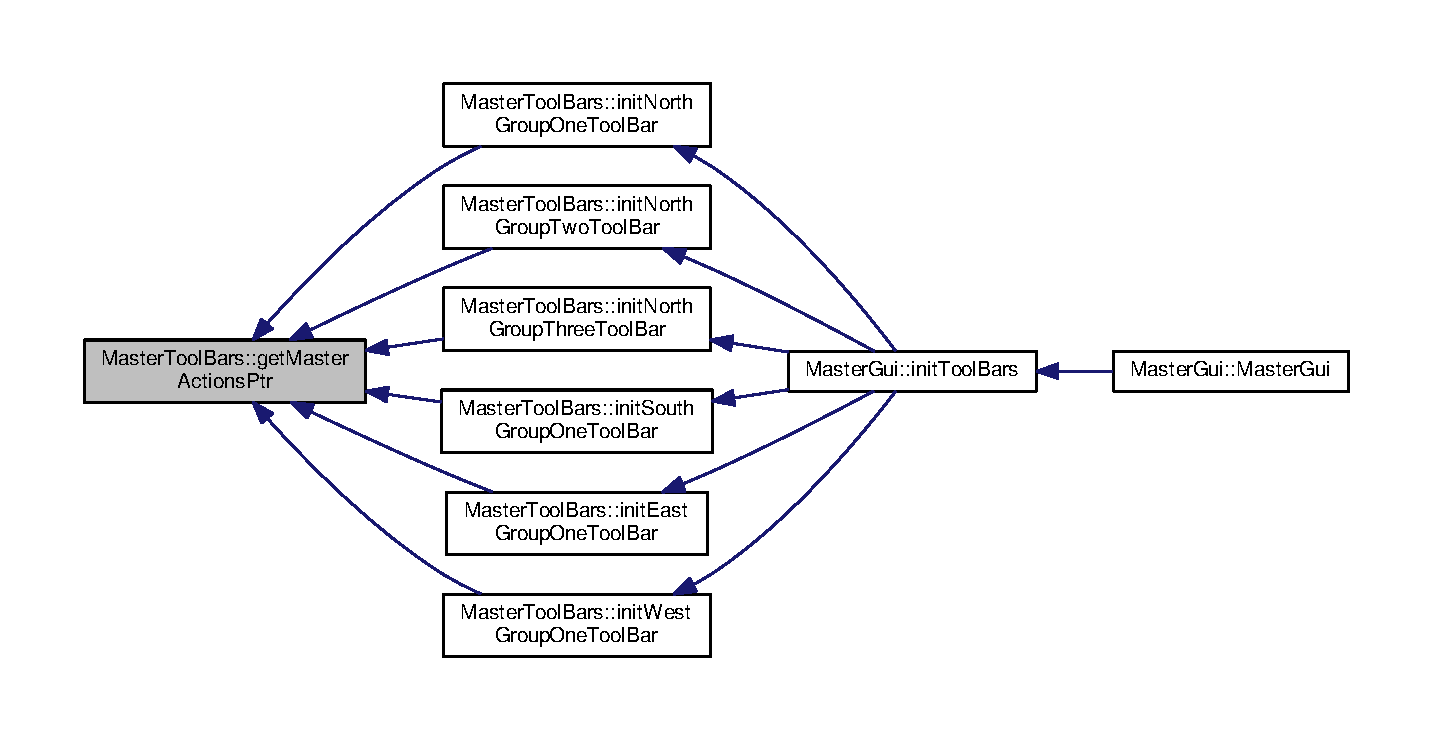
\includegraphics[width=350pt]{class_master_tool_bars_ae73d5e7f4b317e7402ed0b7f6e405fb9_icgraph}
\end{center}
\end{figure}


\hypertarget{class_master_tool_bars_ad17aa8fcdbbbc16c67075b5b06db146e}{\index{Master\-Tool\-Bars@{Master\-Tool\-Bars}!init\-East\-Group\-One\-Tool\-Bar@{init\-East\-Group\-One\-Tool\-Bar}}
\index{init\-East\-Group\-One\-Tool\-Bar@{init\-East\-Group\-One\-Tool\-Bar}!MasterToolBars@{Master\-Tool\-Bars}}
\subsubsection[{init\-East\-Group\-One\-Tool\-Bar}]{\setlength{\rightskip}{0pt plus 5cm}void Master\-Tool\-Bars\-::init\-East\-Group\-One\-Tool\-Bar (
\begin{DoxyParamCaption}
\item[{Q\-Tool\-Bar $\ast$}]{toolbar\-Ptr}
\end{DoxyParamCaption}
)}}\label{class_master_tool_bars_ad17aa8fcdbbbc16c67075b5b06db146e}


Definition at line 58 of file Master\-Tool\-Bars.\-cpp.



Here is the call graph for this function\-:
\nopagebreak
\begin{figure}[H]
\begin{center}
\leavevmode
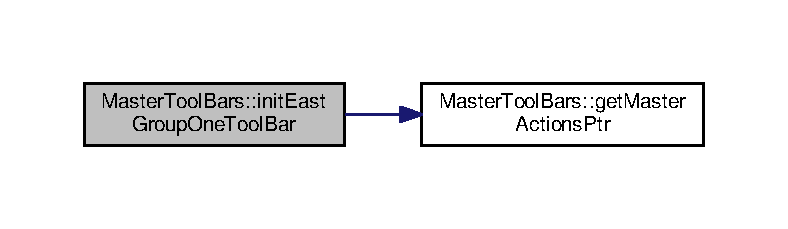
\includegraphics[width=350pt]{class_master_tool_bars_ad17aa8fcdbbbc16c67075b5b06db146e_cgraph}
\end{center}
\end{figure}




Here is the caller graph for this function\-:
\nopagebreak
\begin{figure}[H]
\begin{center}
\leavevmode
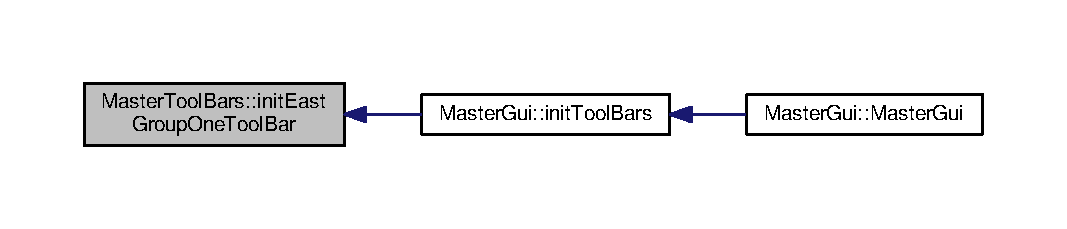
\includegraphics[width=350pt]{class_master_tool_bars_ad17aa8fcdbbbc16c67075b5b06db146e_icgraph}
\end{center}
\end{figure}


\hypertarget{class_master_tool_bars_aec0df27e89d0bbcf5c7b5fc7d2fa8195}{\index{Master\-Tool\-Bars@{Master\-Tool\-Bars}!init\-North\-Group\-One\-Tool\-Bar@{init\-North\-Group\-One\-Tool\-Bar}}
\index{init\-North\-Group\-One\-Tool\-Bar@{init\-North\-Group\-One\-Tool\-Bar}!MasterToolBars@{Master\-Tool\-Bars}}
\subsubsection[{init\-North\-Group\-One\-Tool\-Bar}]{\setlength{\rightskip}{0pt plus 5cm}void Master\-Tool\-Bars\-::init\-North\-Group\-One\-Tool\-Bar (
\begin{DoxyParamCaption}
\item[{Q\-Tool\-Bar $\ast$}]{toolbar\-Ptr}
\end{DoxyParamCaption}
)}}\label{class_master_tool_bars_aec0df27e89d0bbcf5c7b5fc7d2fa8195}


Definition at line 21 of file Master\-Tool\-Bars.\-cpp.



Here is the call graph for this function\-:
\nopagebreak
\begin{figure}[H]
\begin{center}
\leavevmode
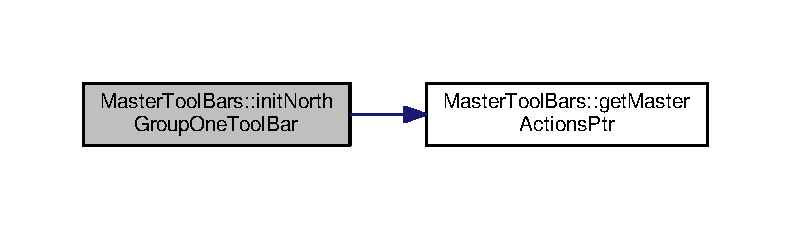
\includegraphics[width=350pt]{class_master_tool_bars_aec0df27e89d0bbcf5c7b5fc7d2fa8195_cgraph}
\end{center}
\end{figure}




Here is the caller graph for this function\-:
\nopagebreak
\begin{figure}[H]
\begin{center}
\leavevmode
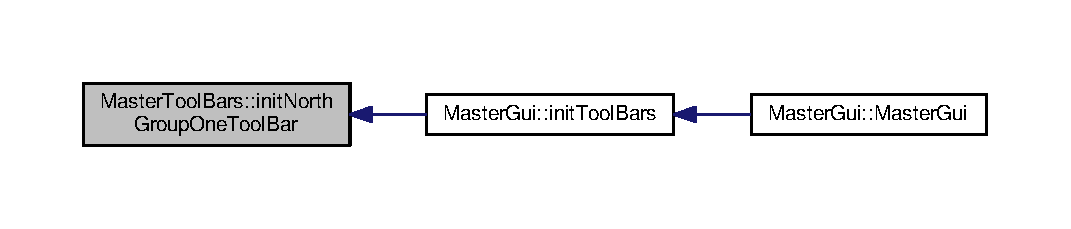
\includegraphics[width=350pt]{class_master_tool_bars_aec0df27e89d0bbcf5c7b5fc7d2fa8195_icgraph}
\end{center}
\end{figure}


\hypertarget{class_master_tool_bars_a058d8e043fc2d5303e21f993c48bc581}{\index{Master\-Tool\-Bars@{Master\-Tool\-Bars}!init\-North\-Group\-Three\-Tool\-Bar@{init\-North\-Group\-Three\-Tool\-Bar}}
\index{init\-North\-Group\-Three\-Tool\-Bar@{init\-North\-Group\-Three\-Tool\-Bar}!MasterToolBars@{Master\-Tool\-Bars}}
\subsubsection[{init\-North\-Group\-Three\-Tool\-Bar}]{\setlength{\rightskip}{0pt plus 5cm}void Master\-Tool\-Bars\-::init\-North\-Group\-Three\-Tool\-Bar (
\begin{DoxyParamCaption}
\item[{Q\-Tool\-Bar $\ast$}]{toolbar\-Ptr}
\end{DoxyParamCaption}
)}}\label{class_master_tool_bars_a058d8e043fc2d5303e21f993c48bc581}


Definition at line 38 of file Master\-Tool\-Bars.\-cpp.



Here is the call graph for this function\-:
\nopagebreak
\begin{figure}[H]
\begin{center}
\leavevmode
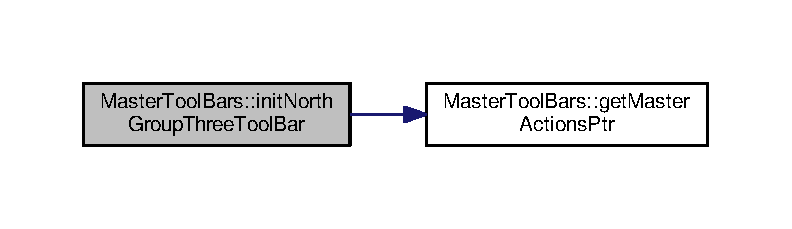
\includegraphics[width=350pt]{class_master_tool_bars_a058d8e043fc2d5303e21f993c48bc581_cgraph}
\end{center}
\end{figure}




Here is the caller graph for this function\-:
\nopagebreak
\begin{figure}[H]
\begin{center}
\leavevmode
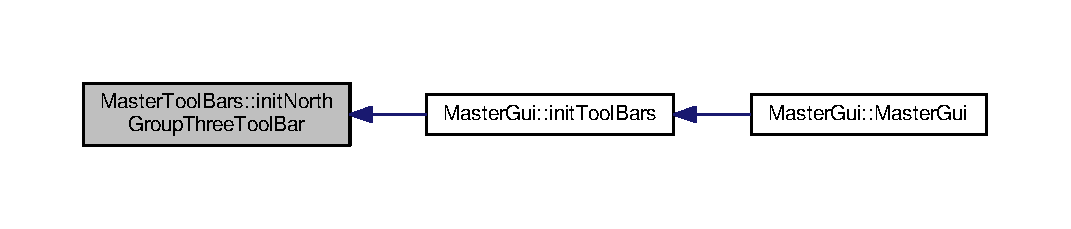
\includegraphics[width=350pt]{class_master_tool_bars_a058d8e043fc2d5303e21f993c48bc581_icgraph}
\end{center}
\end{figure}


\hypertarget{class_master_tool_bars_a6b77ec9af9c57217657689b6564f1a54}{\index{Master\-Tool\-Bars@{Master\-Tool\-Bars}!init\-North\-Group\-Two\-Tool\-Bar@{init\-North\-Group\-Two\-Tool\-Bar}}
\index{init\-North\-Group\-Two\-Tool\-Bar@{init\-North\-Group\-Two\-Tool\-Bar}!MasterToolBars@{Master\-Tool\-Bars}}
\subsubsection[{init\-North\-Group\-Two\-Tool\-Bar}]{\setlength{\rightskip}{0pt plus 5cm}void Master\-Tool\-Bars\-::init\-North\-Group\-Two\-Tool\-Bar (
\begin{DoxyParamCaption}
\item[{Q\-Tool\-Bar $\ast$}]{toolbar\-Ptr}
\end{DoxyParamCaption}
)}}\label{class_master_tool_bars_a6b77ec9af9c57217657689b6564f1a54}


Definition at line 31 of file Master\-Tool\-Bars.\-cpp.



Here is the call graph for this function\-:
\nopagebreak
\begin{figure}[H]
\begin{center}
\leavevmode
\includegraphics[width=350pt]{class_master_tool_bars_a6b77ec9af9c57217657689b6564f1a54_cgraph}
\end{center}
\end{figure}




Here is the caller graph for this function\-:
\nopagebreak
\begin{figure}[H]
\begin{center}
\leavevmode
\includegraphics[width=350pt]{class_master_tool_bars_a6b77ec9af9c57217657689b6564f1a54_icgraph}
\end{center}
\end{figure}


\hypertarget{class_master_tool_bars_a3f8d953232c3c8ad2205913514a7233e}{\index{Master\-Tool\-Bars@{Master\-Tool\-Bars}!init\-South\-Group\-One\-Tool\-Bar@{init\-South\-Group\-One\-Tool\-Bar}}
\index{init\-South\-Group\-One\-Tool\-Bar@{init\-South\-Group\-One\-Tool\-Bar}!MasterToolBars@{Master\-Tool\-Bars}}
\subsubsection[{init\-South\-Group\-One\-Tool\-Bar}]{\setlength{\rightskip}{0pt plus 5cm}void Master\-Tool\-Bars\-::init\-South\-Group\-One\-Tool\-Bar (
\begin{DoxyParamCaption}
\item[{Q\-Tool\-Bar $\ast$}]{toolbar\-Ptr}
\end{DoxyParamCaption}
)}}\label{class_master_tool_bars_a3f8d953232c3c8ad2205913514a7233e}


Definition at line 50 of file Master\-Tool\-Bars.\-cpp.



Here is the call graph for this function\-:
\nopagebreak
\begin{figure}[H]
\begin{center}
\leavevmode
\includegraphics[width=350pt]{class_master_tool_bars_a3f8d953232c3c8ad2205913514a7233e_cgraph}
\end{center}
\end{figure}




Here is the caller graph for this function\-:
\nopagebreak
\begin{figure}[H]
\begin{center}
\leavevmode
\includegraphics[width=350pt]{class_master_tool_bars_a3f8d953232c3c8ad2205913514a7233e_icgraph}
\end{center}
\end{figure}


\hypertarget{class_master_tool_bars_a12bb3e3171d9ea6a6c9cd9c7b800e0d7}{\index{Master\-Tool\-Bars@{Master\-Tool\-Bars}!init\-West\-Group\-One\-Tool\-Bar@{init\-West\-Group\-One\-Tool\-Bar}}
\index{init\-West\-Group\-One\-Tool\-Bar@{init\-West\-Group\-One\-Tool\-Bar}!MasterToolBars@{Master\-Tool\-Bars}}
\subsubsection[{init\-West\-Group\-One\-Tool\-Bar}]{\setlength{\rightskip}{0pt plus 5cm}void Master\-Tool\-Bars\-::init\-West\-Group\-One\-Tool\-Bar (
\begin{DoxyParamCaption}
\item[{Q\-Tool\-Bar $\ast$}]{toolbar\-Ptr}
\end{DoxyParamCaption}
)}}\label{class_master_tool_bars_a12bb3e3171d9ea6a6c9cd9c7b800e0d7}


Definition at line 64 of file Master\-Tool\-Bars.\-cpp.



Here is the call graph for this function\-:
\nopagebreak
\begin{figure}[H]
\begin{center}
\leavevmode
\includegraphics[width=350pt]{class_master_tool_bars_a12bb3e3171d9ea6a6c9cd9c7b800e0d7_cgraph}
\end{center}
\end{figure}




Here is the caller graph for this function\-:
\nopagebreak
\begin{figure}[H]
\begin{center}
\leavevmode
\includegraphics[width=350pt]{class_master_tool_bars_a12bb3e3171d9ea6a6c9cd9c7b800e0d7_icgraph}
\end{center}
\end{figure}


\hypertarget{class_master_tool_bars_a8cc2c4f46779f429221b1dee8ad58181}{\index{Master\-Tool\-Bars@{Master\-Tool\-Bars}!set\-Master\-Actions\-Ptr@{set\-Master\-Actions\-Ptr}}
\index{set\-Master\-Actions\-Ptr@{set\-Master\-Actions\-Ptr}!MasterToolBars@{Master\-Tool\-Bars}}
\subsubsection[{set\-Master\-Actions\-Ptr}]{\setlength{\rightskip}{0pt plus 5cm}void Master\-Tool\-Bars\-::set\-Master\-Actions\-Ptr (
\begin{DoxyParamCaption}
\item[{{\bf Master\-Actions} $\ast$}]{master\-Actions\-Ptr}
\end{DoxyParamCaption}
)}}\label{class_master_tool_bars_a8cc2c4f46779f429221b1dee8ad58181}


Definition at line 9 of file Master\-Tool\-Bars.\-cpp.



Here is the caller graph for this function\-:
\nopagebreak
\begin{figure}[H]
\begin{center}
\leavevmode
\includegraphics[width=350pt]{class_master_tool_bars_a8cc2c4f46779f429221b1dee8ad58181_icgraph}
\end{center}
\end{figure}




\subsection{Member Data Documentation}
\hypertarget{class_master_tool_bars_a1adde6a67eaa64fbbbf65ffcb8c1590f}{\index{Master\-Tool\-Bars@{Master\-Tool\-Bars}!master\-Actions@{master\-Actions}}
\index{master\-Actions@{master\-Actions}!MasterToolBars@{Master\-Tool\-Bars}}
\subsubsection[{master\-Actions}]{\setlength{\rightskip}{0pt plus 5cm}{\bf Master\-Actions}$\ast$ Master\-Tool\-Bars\-::master\-Actions\hspace{0.3cm}{\ttfamily [private]}}}\label{class_master_tool_bars_a1adde6a67eaa64fbbbf65ffcb8c1590f}


Definition at line 29 of file Master\-Tool\-Bars.\-h.



The documentation for this class was generated from the following files\-:\begin{DoxyCompactItemize}
\item 
/home/james/\-Net\-Beans\-Projects/ride/src/\hyperlink{_master_tool_bars_8h}{Master\-Tool\-Bars.\-h}\item 
/home/james/\-Net\-Beans\-Projects/ride/src/\hyperlink{_master_tool_bars_8cpp}{Master\-Tool\-Bars.\-cpp}\end{DoxyCompactItemize}

\hypertarget{class_navigator_gui}{\section{Navigator\-Gui Class Reference}
\label{class_navigator_gui}\index{Navigator\-Gui@{Navigator\-Gui}}
}


{\ttfamily \#include $<$Navigator\-Gui.\-h$>$}



Inheritance diagram for Navigator\-Gui\-:
\nopagebreak
\begin{figure}[H]
\begin{center}
\leavevmode
\includegraphics[width=154pt]{class_navigator_gui__inherit__graph}
\end{center}
\end{figure}


Collaboration diagram for Navigator\-Gui\-:
\nopagebreak
\begin{figure}[H]
\begin{center}
\leavevmode
\includegraphics[width=245pt]{class_navigator_gui__coll__graph}
\end{center}
\end{figure}
\subsection*{Public Member Functions}
\begin{DoxyCompactItemize}
\item 
\hyperlink{class_navigator_gui_ac7a57ace6bc543313233afffe9a9073b}{Navigator\-Gui} (Q\-Widget $\ast$parent=0)
\item 
void \hyperlink{class_navigator_gui_a318115279c155077854f5126d290b2b7}{load\-Data} ()
\item 
void \hyperlink{class_navigator_gui_a3d5d2c50735ed741cad32790b6ed8778}{set\-West\-Tab\-Widget\-Ptr} (Q\-Tab\-Widget $\ast$master\-Tab\-Widget\-Ptr)
\item 
Q\-Tab\-Widget $\ast$ \hyperlink{class_navigator_gui_a3eeb5652b2351ecb1988c17ee857c9cf}{get\-West\-Tab\-Widget\-Ptr} ()
\item 
\hyperlink{class_navigator_gui_a8fc032fe6ad4c935a14ba22853191285}{$\sim$\-Navigator\-Gui} ()
\end{DoxyCompactItemize}
\subsection*{Private Attributes}
\begin{DoxyCompactItemize}
\item 
Q\-List\-Widget $\ast$ \hyperlink{class_navigator_gui_aa3732fbecbd29c6a22eaebe82bb57af7}{list\-Widget\-Ptr}
\item 
\hyperlink{class_search_widget}{Search\-Widget} $\ast$ \hyperlink{class_navigator_gui_a33531deedb97ceb340409fc4e5f8620e}{search\-Widget\-Ptr}
\item 
Q\-Push\-Button $\ast$ \hyperlink{class_navigator_gui_a8256fec3fdcad7fea838c7ba701e3d6e}{activate\-Search\-Btn}
\item 
Q\-String $\ast$ \hyperlink{class_navigator_gui_aa233c8e6f7634b4de98b2dcaaa86ed69}{file\-Str\-Ptr}
\item 
Q\-Tab\-Widget $\ast$ \hyperlink{class_navigator_gui_aea3dc7b54a723ca369742ee6a0f34f03}{west\-Tab\-Widget\-Ptr}
\item 
Q\-Grid\-Layout $\ast$ \hyperlink{class_navigator_gui_a0e981a409e2879e799f5e05e0c695f4a}{outer\-Layout}
\end{DoxyCompactItemize}


\subsection{Detailed Description}


Definition at line 26 of file Navigator\-Gui.\-h.



\subsection{Constructor \& Destructor Documentation}
\hypertarget{class_navigator_gui_ac7a57ace6bc543313233afffe9a9073b}{\index{Navigator\-Gui@{Navigator\-Gui}!Navigator\-Gui@{Navigator\-Gui}}
\index{Navigator\-Gui@{Navigator\-Gui}!NavigatorGui@{Navigator\-Gui}}
\subsubsection[{Navigator\-Gui}]{\setlength{\rightskip}{0pt plus 5cm}Navigator\-Gui\-::\-Navigator\-Gui (
\begin{DoxyParamCaption}
\item[{Q\-Widget $\ast$}]{parent = {\ttfamily 0}}
\end{DoxyParamCaption}
)}}\label{class_navigator_gui_ac7a57ace6bc543313233afffe9a9073b}


Definition at line 4 of file Navigator\-Gui.\-cpp.

\hypertarget{class_navigator_gui_a8fc032fe6ad4c935a14ba22853191285}{\index{Navigator\-Gui@{Navigator\-Gui}!$\sim$\-Navigator\-Gui@{$\sim$\-Navigator\-Gui}}
\index{$\sim$\-Navigator\-Gui@{$\sim$\-Navigator\-Gui}!NavigatorGui@{Navigator\-Gui}}
\subsubsection[{$\sim$\-Navigator\-Gui}]{\setlength{\rightskip}{0pt plus 5cm}Navigator\-Gui\-::$\sim$\-Navigator\-Gui (
\begin{DoxyParamCaption}
{}
\end{DoxyParamCaption}
)}}\label{class_navigator_gui_a8fc032fe6ad4c935a14ba22853191285}


Definition at line 39 of file Navigator\-Gui.\-cpp.



\subsection{Member Function Documentation}
\hypertarget{class_navigator_gui_a3eeb5652b2351ecb1988c17ee857c9cf}{\index{Navigator\-Gui@{Navigator\-Gui}!get\-West\-Tab\-Widget\-Ptr@{get\-West\-Tab\-Widget\-Ptr}}
\index{get\-West\-Tab\-Widget\-Ptr@{get\-West\-Tab\-Widget\-Ptr}!NavigatorGui@{Navigator\-Gui}}
\subsubsection[{get\-West\-Tab\-Widget\-Ptr}]{\setlength{\rightskip}{0pt plus 5cm}Q\-Tab\-Widget $\ast$ Navigator\-Gui\-::get\-West\-Tab\-Widget\-Ptr (
\begin{DoxyParamCaption}
{}
\end{DoxyParamCaption}
)}}\label{class_navigator_gui_a3eeb5652b2351ecb1988c17ee857c9cf}


Definition at line 33 of file Navigator\-Gui.\-cpp.

\hypertarget{class_navigator_gui_a318115279c155077854f5126d290b2b7}{\index{Navigator\-Gui@{Navigator\-Gui}!load\-Data@{load\-Data}}
\index{load\-Data@{load\-Data}!NavigatorGui@{Navigator\-Gui}}
\subsubsection[{load\-Data}]{\setlength{\rightskip}{0pt plus 5cm}void Navigator\-Gui\-::load\-Data (
\begin{DoxyParamCaption}
{}
\end{DoxyParamCaption}
)}}\label{class_navigator_gui_a318115279c155077854f5126d290b2b7}


Definition at line 21 of file Navigator\-Gui.\-cpp.

\hypertarget{class_navigator_gui_a3d5d2c50735ed741cad32790b6ed8778}{\index{Navigator\-Gui@{Navigator\-Gui}!set\-West\-Tab\-Widget\-Ptr@{set\-West\-Tab\-Widget\-Ptr}}
\index{set\-West\-Tab\-Widget\-Ptr@{set\-West\-Tab\-Widget\-Ptr}!NavigatorGui@{Navigator\-Gui}}
\subsubsection[{set\-West\-Tab\-Widget\-Ptr}]{\setlength{\rightskip}{0pt plus 5cm}void Navigator\-Gui\-::set\-West\-Tab\-Widget\-Ptr (
\begin{DoxyParamCaption}
\item[{Q\-Tab\-Widget $\ast$}]{master\-Tab\-Widget\-Ptr}
\end{DoxyParamCaption}
)}}\label{class_navigator_gui_a3d5d2c50735ed741cad32790b6ed8778}


Definition at line 27 of file Navigator\-Gui.\-cpp.



\subsection{Member Data Documentation}
\hypertarget{class_navigator_gui_a8256fec3fdcad7fea838c7ba701e3d6e}{\index{Navigator\-Gui@{Navigator\-Gui}!activate\-Search\-Btn@{activate\-Search\-Btn}}
\index{activate\-Search\-Btn@{activate\-Search\-Btn}!NavigatorGui@{Navigator\-Gui}}
\subsubsection[{activate\-Search\-Btn}]{\setlength{\rightskip}{0pt plus 5cm}Q\-Push\-Button$\ast$ Navigator\-Gui\-::activate\-Search\-Btn\hspace{0.3cm}{\ttfamily [private]}}}\label{class_navigator_gui_a8256fec3fdcad7fea838c7ba701e3d6e}


Definition at line 33 of file Navigator\-Gui.\-h.

\hypertarget{class_navigator_gui_aa233c8e6f7634b4de98b2dcaaa86ed69}{\index{Navigator\-Gui@{Navigator\-Gui}!file\-Str\-Ptr@{file\-Str\-Ptr}}
\index{file\-Str\-Ptr@{file\-Str\-Ptr}!NavigatorGui@{Navigator\-Gui}}
\subsubsection[{file\-Str\-Ptr}]{\setlength{\rightskip}{0pt plus 5cm}Q\-String$\ast$ Navigator\-Gui\-::file\-Str\-Ptr\hspace{0.3cm}{\ttfamily [private]}}}\label{class_navigator_gui_aa233c8e6f7634b4de98b2dcaaa86ed69}


Definition at line 34 of file Navigator\-Gui.\-h.

\hypertarget{class_navigator_gui_aa3732fbecbd29c6a22eaebe82bb57af7}{\index{Navigator\-Gui@{Navigator\-Gui}!list\-Widget\-Ptr@{list\-Widget\-Ptr}}
\index{list\-Widget\-Ptr@{list\-Widget\-Ptr}!NavigatorGui@{Navigator\-Gui}}
\subsubsection[{list\-Widget\-Ptr}]{\setlength{\rightskip}{0pt plus 5cm}Q\-List\-Widget$\ast$ Navigator\-Gui\-::list\-Widget\-Ptr\hspace{0.3cm}{\ttfamily [private]}}}\label{class_navigator_gui_aa3732fbecbd29c6a22eaebe82bb57af7}


Definition at line 31 of file Navigator\-Gui.\-h.

\hypertarget{class_navigator_gui_a0e981a409e2879e799f5e05e0c695f4a}{\index{Navigator\-Gui@{Navigator\-Gui}!outer\-Layout@{outer\-Layout}}
\index{outer\-Layout@{outer\-Layout}!NavigatorGui@{Navigator\-Gui}}
\subsubsection[{outer\-Layout}]{\setlength{\rightskip}{0pt plus 5cm}Q\-Grid\-Layout$\ast$ Navigator\-Gui\-::outer\-Layout\hspace{0.3cm}{\ttfamily [private]}}}\label{class_navigator_gui_a0e981a409e2879e799f5e05e0c695f4a}


Definition at line 37 of file Navigator\-Gui.\-h.

\hypertarget{class_navigator_gui_a33531deedb97ceb340409fc4e5f8620e}{\index{Navigator\-Gui@{Navigator\-Gui}!search\-Widget\-Ptr@{search\-Widget\-Ptr}}
\index{search\-Widget\-Ptr@{search\-Widget\-Ptr}!NavigatorGui@{Navigator\-Gui}}
\subsubsection[{search\-Widget\-Ptr}]{\setlength{\rightskip}{0pt plus 5cm}{\bf Search\-Widget}$\ast$ Navigator\-Gui\-::search\-Widget\-Ptr\hspace{0.3cm}{\ttfamily [private]}}}\label{class_navigator_gui_a33531deedb97ceb340409fc4e5f8620e}


Definition at line 32 of file Navigator\-Gui.\-h.

\hypertarget{class_navigator_gui_aea3dc7b54a723ca369742ee6a0f34f03}{\index{Navigator\-Gui@{Navigator\-Gui}!west\-Tab\-Widget\-Ptr@{west\-Tab\-Widget\-Ptr}}
\index{west\-Tab\-Widget\-Ptr@{west\-Tab\-Widget\-Ptr}!NavigatorGui@{Navigator\-Gui}}
\subsubsection[{west\-Tab\-Widget\-Ptr}]{\setlength{\rightskip}{0pt plus 5cm}Q\-Tab\-Widget$\ast$ Navigator\-Gui\-::west\-Tab\-Widget\-Ptr\hspace{0.3cm}{\ttfamily [private]}}}\label{class_navigator_gui_aea3dc7b54a723ca369742ee6a0f34f03}


Definition at line 36 of file Navigator\-Gui.\-h.



The documentation for this class was generated from the following files\-:\begin{DoxyCompactItemize}
\item 
/home/james/\-Net\-Beans\-Projects/ride/src/\hyperlink{_navigator_gui_8h}{Navigator\-Gui.\-h}\item 
/home/james/\-Net\-Beans\-Projects/ride/src/\hyperlink{_navigator_gui_8cpp}{Navigator\-Gui.\-cpp}\end{DoxyCompactItemize}

\hypertarget{class_new_file_gui}{\section{New\-File\-Gui Class Reference}
\label{class_new_file_gui}\index{New\-File\-Gui@{New\-File\-Gui}}
}


{\ttfamily \#include $<$New\-File\-Gui.\-h$>$}



Inheritance diagram for New\-File\-Gui\-:\nopagebreak
\begin{figure}[H]
\begin{center}
\leavevmode
\includegraphics[width=148pt]{class_new_file_gui__inherit__graph}
\end{center}
\end{figure}


Collaboration diagram for New\-File\-Gui\-:\nopagebreak
\begin{figure}[H]
\begin{center}
\leavevmode
\includegraphics[width=350pt]{class_new_file_gui__coll__graph}
\end{center}
\end{figure}
\subsection*{Public Member Functions}
\begin{DoxyCompactItemize}
\item 
\hyperlink{class_new_file_gui_a090f156ef13c1915fe96cd47f6ff049d}{New\-File\-Gui} (Q\-Widget $\ast$parent=0)
\item 
void \hyperlink{class_new_file_gui_ad4a8eb0dc938398749073e636bd7fc3f}{set\-Master\-Tab\-Widget\-Ptr} (Q\-Tab\-Widget $\ast$\hyperlink{class_new_file_gui_a9a3baa00763c6d8d90e7e39ea3f1585c}{master\-Tab\-Widget\-Ptr})
\item 
Q\-Tab\-Widget $\ast$ \hyperlink{class_new_file_gui_a650227edbbc789784a56b2f990697abb}{get\-Master\-Tab\-Widget\-Ptr} ()
\item 
void \hyperlink{class_new_file_gui_ac35f4e742681ccc0d52d083899b4bc85}{set\-Highlighter\-Ptr} (\hyperlink{class_highlighter}{Highlighter} $\ast$\hyperlink{class_new_file_gui_a4a63ed16985eeb14fbe35e3197420873}{highlighter\-Ptr})
\item 
\hyperlink{class_highlighter}{Highlighter} $\ast$ \hyperlink{class_new_file_gui_a51fe16ba94f7089b4b5961d30053e1f7}{get\-Highlighter\-Ptr} ()
\item 
void \hyperlink{class_new_file_gui_ad77edffa59956f16ef2b6d83dd357932}{init\-Btns} ()
\item 
void \hyperlink{class_new_file_gui_a3789c0137a7a1e6d3b9a09ebf97657c5}{swap\-Next\-Page} ()
\item 
void \hyperlink{class_new_file_gui_a19b6c2a372c842aa72b244b11fe458e7}{swap\-Back\-Page} ()
\item 
void \hyperlink{class_new_file_gui_ae279a6aa9f6e065254f02595491870bf}{load\-Page\-\_\-1} ()
\item 
void \hyperlink{class_new_file_gui_ac5098fcfded5a9fca609eef19a777a46}{unload\-Page\-\_\-1} ()
\item 
void \hyperlink{class_new_file_gui_a734dbe5493abf2d090b331c9b5d3ea39}{load\-Page\-\_\-2} ()
\item 
void \hyperlink{class_new_file_gui_a38230b8cf285f610595f9e762be4a3ba}{unload\-Page\-\_\-2} ()
\item 
void \hyperlink{class_new_file_gui_a7f61834fa8074aeefebfcb8600bba8cd}{load\-Page\-\_\-3} ()
\item 
void \hyperlink{class_new_file_gui_a7ef65bd194d94091ff27648f765023b6}{unload\-Page\-\_\-3} ()
\item 
void \hyperlink{class_new_file_gui_ad60fb0b561d16f76062af7e17732d318}{load\-Page\-\_\-4} ()
\item 
void \hyperlink{class_new_file_gui_a7f604bc4692d3ebd66d00544fb1eb2de}{unload\-Page\-\_\-4} ()
\item 
Q\-String $\ast$ \hyperlink{class_new_file_gui_a521fe1c6fd4fbbbe2b28050e77f772a1}{to\-String} ()
\item 
\hyperlink{class_new_file_gui_aaaa64713298564b96e77a199a911c27b}{$\sim$\-New\-File\-Gui} ()
\end{DoxyCompactItemize}
\subsection*{Private Types}
\begin{DoxyCompactItemize}
\item 
enum \hyperlink{class_new_file_gui_aa420702f51dbeefc704d546f1db144ac}{Page} \{ \hyperlink{class_new_file_gui_aa420702f51dbeefc704d546f1db144acab331f50bb023c696186edd5033b87462}{P\-A\-G\-E\-\_\-\-O\-N\-E}, 
\hyperlink{class_new_file_gui_aa420702f51dbeefc704d546f1db144aca80e5a1b1a11c76c1813a66e5742336dc}{P\-A\-G\-E\-\_\-\-T\-W\-O}, 
\hyperlink{class_new_file_gui_aa420702f51dbeefc704d546f1db144aca20553a422680bc600e39dcbd9615273f}{P\-A\-G\-E\-\_\-\-T\-H\-R\-E\-E}, 
\hyperlink{class_new_file_gui_aa420702f51dbeefc704d546f1db144aca3e2121cb48d9c9adbec8732efcc8de1e}{P\-A\-G\-E\-\_\-\-F\-O\-U\-R}
 \}
\end{DoxyCompactItemize}
\subsection*{Private Slots}
\begin{DoxyCompactItemize}
\item 
void \hyperlink{class_new_file_gui_a0026dbfc8bd314dc7d0a90ef23995724}{handle\-Back\-Btn\-Slot} ()
\item 
void \hyperlink{class_new_file_gui_ac5ff3b20c4c0a6b863a220073dc232d9}{handle\-Next\-Btn\-Slot} ()
\item 
void \hyperlink{class_new_file_gui_a50cf414bdb9ea40f3cd4ca4fa4566b77}{handle\-Finish\-Btn\-Slot} ()
\item 
void \hyperlink{class_new_file_gui_a32ecca09a47e1ee6d8619e4d6d8c10be}{handle\-Help\-Bnt\-Slot} ()
\item 
void \hyperlink{class_new_file_gui_a137c2e64fa0cebe11c92bd38be955be5}{handle\-Cancel\-Btn\-Slot} ()
\end{DoxyCompactItemize}
\subsection*{Private Member Functions}
\begin{DoxyCompactItemize}
\item 
Q\-Abstract\-Item\-Model $\ast$ \hyperlink{class_new_file_gui_a4ff330f407388321ba41817b3b3c8240}{model\-From\-File} (const Q\-String \&file\-Name)
\end{DoxyCompactItemize}
\subsection*{Private Attributes}
\begin{DoxyCompactItemize}
\item 
\hyperlink{class_new_file_gui_aa420702f51dbeefc704d546f1db144ac}{Page} \hyperlink{class_new_file_gui_adaf414f47f140c24e8f08797262c646b}{current\-Page}
\item 
Q\-Push\-Button $\ast$ \hyperlink{class_new_file_gui_a795eb9a1d91260f9f99b15b8544e71e6}{back\-Btn}
\item 
Q\-Push\-Button $\ast$ \hyperlink{class_new_file_gui_ad1fa3cb3fa909bf6e71672497350f980}{next\-Btn}
\item 
Q\-Push\-Button $\ast$ \hyperlink{class_new_file_gui_a9caaf4a098bc03388235461844770705}{finish\-Btn}
\item 
Q\-Push\-Button $\ast$ \hyperlink{class_new_file_gui_a3a59cd57999cc1004a95ab2fbb3e6766}{help\-Btn}
\item 
Q\-Push\-Button $\ast$ \hyperlink{class_new_file_gui_a5be4525cfa97c2ec799a7357eb6a1fb4}{cancel\-Btn}
\item 
Q\-Grid\-Layout $\ast$ \hyperlink{class_new_file_gui_ae5aa1370799c06f4368ef636279ab259}{outer\-Layout}
\item 
Q\-H\-Box\-Layout $\ast$ \hyperlink{class_new_file_gui_aec890bfe56498ad4c1e3865387f147b5}{button\-Layout}
\item 
Q\-Tab\-Widget $\ast$ \hyperlink{class_new_file_gui_a9a3baa00763c6d8d90e7e39ea3f1585c}{master\-Tab\-Widget\-Ptr}
\item 
\hyperlink{class_highlighter}{Highlighter} $\ast$ \hyperlink{class_new_file_gui_a4a63ed16985eeb14fbe35e3197420873}{highlighter\-Ptr}
\item 
\hyperlink{class_file_gui}{File\-Gui} $\ast$ \hyperlink{class_new_file_gui_a7521ff2d2934c4a19fbef21a3a034ee9}{editor}
\item 
Q\-Completer $\ast$ \hyperlink{class_new_file_gui_a5c8508fb9dba194838e0cfce4d6f7988}{completer}
\item 
\hyperlink{class_new_file_page__1}{New\-File\-Page\-\_\-1} $\ast$ \hyperlink{class_new_file_gui_afdeb5fdcb313e360f1479a5fd3553e4b}{new\-File\-Page\-\_\-1\-Ptr}
\item 
\hyperlink{class_new_file_page__2}{New\-File\-Page\-\_\-2} $\ast$ \hyperlink{class_new_file_gui_ad976d235939ccda48373c3a1ced35341}{new\-File\-Page\-\_\-2\-Ptr}
\item 
\hyperlink{class_new_file_page__3}{New\-File\-Page\-\_\-3} $\ast$ \hyperlink{class_new_file_gui_a2a6f8c88d96686a0e84c537bb9b77f09}{new\-File\-Page\-\_\-3\-Ptr}
\item 
\hyperlink{class_new_file_page__4}{New\-File\-Page\-\_\-4} $\ast$ \hyperlink{class_new_file_gui_a5b83d6fcae79fb5da3677848ec49647f}{new\-File\-Page\-\_\-4\-Ptr}
\end{DoxyCompactItemize}


\subsection{Detailed Description}


Definition at line 44 of file New\-File\-Gui.\-h.



\subsection{Member Enumeration Documentation}
\hypertarget{class_new_file_gui_aa420702f51dbeefc704d546f1db144ac}{\index{New\-File\-Gui@{New\-File\-Gui}!Page@{Page}}
\index{Page@{Page}!NewFileGui@{New\-File\-Gui}}
\subsubsection[{Page}]{\setlength{\rightskip}{0pt plus 5cm}enum {\bf New\-File\-Gui\-::\-Page}\hspace{0.3cm}{\ttfamily [private]}}}\label{class_new_file_gui_aa420702f51dbeefc704d546f1db144ac}
\begin{Desc}
\item[Enumerator]\par
\begin{description}
\index{P\-A\-G\-E\-\_\-\-O\-N\-E@{P\-A\-G\-E\-\_\-\-O\-N\-E}!New\-File\-Gui@{New\-File\-Gui}}\index{New\-File\-Gui@{New\-File\-Gui}!P\-A\-G\-E\-\_\-\-O\-N\-E@{P\-A\-G\-E\-\_\-\-O\-N\-E}}\item[{\em 
\hypertarget{class_new_file_gui_aa420702f51dbeefc704d546f1db144acab331f50bb023c696186edd5033b87462}{P\-A\-G\-E\-\_\-\-O\-N\-E}\label{class_new_file_gui_aa420702f51dbeefc704d546f1db144acab331f50bb023c696186edd5033b87462}
}]\index{P\-A\-G\-E\-\_\-\-T\-W\-O@{P\-A\-G\-E\-\_\-\-T\-W\-O}!New\-File\-Gui@{New\-File\-Gui}}\index{New\-File\-Gui@{New\-File\-Gui}!P\-A\-G\-E\-\_\-\-T\-W\-O@{P\-A\-G\-E\-\_\-\-T\-W\-O}}\item[{\em 
\hypertarget{class_new_file_gui_aa420702f51dbeefc704d546f1db144aca80e5a1b1a11c76c1813a66e5742336dc}{P\-A\-G\-E\-\_\-\-T\-W\-O}\label{class_new_file_gui_aa420702f51dbeefc704d546f1db144aca80e5a1b1a11c76c1813a66e5742336dc}
}]\index{P\-A\-G\-E\-\_\-\-T\-H\-R\-E\-E@{P\-A\-G\-E\-\_\-\-T\-H\-R\-E\-E}!New\-File\-Gui@{New\-File\-Gui}}\index{New\-File\-Gui@{New\-File\-Gui}!P\-A\-G\-E\-\_\-\-T\-H\-R\-E\-E@{P\-A\-G\-E\-\_\-\-T\-H\-R\-E\-E}}\item[{\em 
\hypertarget{class_new_file_gui_aa420702f51dbeefc704d546f1db144aca20553a422680bc600e39dcbd9615273f}{P\-A\-G\-E\-\_\-\-T\-H\-R\-E\-E}\label{class_new_file_gui_aa420702f51dbeefc704d546f1db144aca20553a422680bc600e39dcbd9615273f}
}]\index{P\-A\-G\-E\-\_\-\-F\-O\-U\-R@{P\-A\-G\-E\-\_\-\-F\-O\-U\-R}!New\-File\-Gui@{New\-File\-Gui}}\index{New\-File\-Gui@{New\-File\-Gui}!P\-A\-G\-E\-\_\-\-F\-O\-U\-R@{P\-A\-G\-E\-\_\-\-F\-O\-U\-R}}\item[{\em 
\hypertarget{class_new_file_gui_aa420702f51dbeefc704d546f1db144aca3e2121cb48d9c9adbec8732efcc8de1e}{P\-A\-G\-E\-\_\-\-F\-O\-U\-R}\label{class_new_file_gui_aa420702f51dbeefc704d546f1db144aca3e2121cb48d9c9adbec8732efcc8de1e}
}]\end{description}
\end{Desc}


Definition at line 49 of file New\-File\-Gui.\-h.



\subsection{Constructor \& Destructor Documentation}
\hypertarget{class_new_file_gui_a090f156ef13c1915fe96cd47f6ff049d}{\index{New\-File\-Gui@{New\-File\-Gui}!New\-File\-Gui@{New\-File\-Gui}}
\index{New\-File\-Gui@{New\-File\-Gui}!NewFileGui@{New\-File\-Gui}}
\subsubsection[{New\-File\-Gui}]{\setlength{\rightskip}{0pt plus 5cm}New\-File\-Gui\-::\-New\-File\-Gui (
\begin{DoxyParamCaption}
\item[{Q\-Widget $\ast$}]{parent = {\ttfamily 0}}
\end{DoxyParamCaption}
)}}\label{class_new_file_gui_a090f156ef13c1915fe96cd47f6ff049d}


Definition at line 5 of file New\-File\-Gui.\-cpp.

\hypertarget{class_new_file_gui_aaaa64713298564b96e77a199a911c27b}{\index{New\-File\-Gui@{New\-File\-Gui}!$\sim$\-New\-File\-Gui@{$\sim$\-New\-File\-Gui}}
\index{$\sim$\-New\-File\-Gui@{$\sim$\-New\-File\-Gui}!NewFileGui@{New\-File\-Gui}}
\subsubsection[{$\sim$\-New\-File\-Gui}]{\setlength{\rightskip}{0pt plus 5cm}New\-File\-Gui\-::$\sim$\-New\-File\-Gui (
\begin{DoxyParamCaption}
{}
\end{DoxyParamCaption}
)}}\label{class_new_file_gui_aaaa64713298564b96e77a199a911c27b}


Definition at line 334 of file New\-File\-Gui.\-cpp.



\subsection{Member Function Documentation}
\hypertarget{class_new_file_gui_a51fe16ba94f7089b4b5961d30053e1f7}{\index{New\-File\-Gui@{New\-File\-Gui}!get\-Highlighter\-Ptr@{get\-Highlighter\-Ptr}}
\index{get\-Highlighter\-Ptr@{get\-Highlighter\-Ptr}!NewFileGui@{New\-File\-Gui}}
\subsubsection[{get\-Highlighter\-Ptr}]{\setlength{\rightskip}{0pt plus 5cm}{\bf Highlighter} $\ast$ New\-File\-Gui\-::get\-Highlighter\-Ptr (
\begin{DoxyParamCaption}
{}
\end{DoxyParamCaption}
)}}\label{class_new_file_gui_a51fe16ba94f7089b4b5961d30053e1f7}


Definition at line 45 of file New\-File\-Gui.\-cpp.

\hypertarget{class_new_file_gui_a650227edbbc789784a56b2f990697abb}{\index{New\-File\-Gui@{New\-File\-Gui}!get\-Master\-Tab\-Widget\-Ptr@{get\-Master\-Tab\-Widget\-Ptr}}
\index{get\-Master\-Tab\-Widget\-Ptr@{get\-Master\-Tab\-Widget\-Ptr}!NewFileGui@{New\-File\-Gui}}
\subsubsection[{get\-Master\-Tab\-Widget\-Ptr}]{\setlength{\rightskip}{0pt plus 5cm}Q\-Tab\-Widget $\ast$ New\-File\-Gui\-::get\-Master\-Tab\-Widget\-Ptr (
\begin{DoxyParamCaption}
{}
\end{DoxyParamCaption}
)}}\label{class_new_file_gui_a650227edbbc789784a56b2f990697abb}


Definition at line 33 of file New\-File\-Gui.\-cpp.

\hypertarget{class_new_file_gui_a0026dbfc8bd314dc7d0a90ef23995724}{\index{New\-File\-Gui@{New\-File\-Gui}!handle\-Back\-Btn\-Slot@{handle\-Back\-Btn\-Slot}}
\index{handle\-Back\-Btn\-Slot@{handle\-Back\-Btn\-Slot}!NewFileGui@{New\-File\-Gui}}
\subsubsection[{handle\-Back\-Btn\-Slot}]{\setlength{\rightskip}{0pt plus 5cm}void New\-File\-Gui\-::handle\-Back\-Btn\-Slot (
\begin{DoxyParamCaption}
{}
\end{DoxyParamCaption}
)\hspace{0.3cm}{\ttfamily [private]}, {\ttfamily [slot]}}}\label{class_new_file_gui_a0026dbfc8bd314dc7d0a90ef23995724}


Definition at line 51 of file New\-File\-Gui.\-cpp.

\hypertarget{class_new_file_gui_a137c2e64fa0cebe11c92bd38be955be5}{\index{New\-File\-Gui@{New\-File\-Gui}!handle\-Cancel\-Btn\-Slot@{handle\-Cancel\-Btn\-Slot}}
\index{handle\-Cancel\-Btn\-Slot@{handle\-Cancel\-Btn\-Slot}!NewFileGui@{New\-File\-Gui}}
\subsubsection[{handle\-Cancel\-Btn\-Slot}]{\setlength{\rightskip}{0pt plus 5cm}void New\-File\-Gui\-::handle\-Cancel\-Btn\-Slot (
\begin{DoxyParamCaption}
{}
\end{DoxyParamCaption}
)\hspace{0.3cm}{\ttfamily [private]}, {\ttfamily [slot]}}}\label{class_new_file_gui_a137c2e64fa0cebe11c92bd38be955be5}


Definition at line 137 of file New\-File\-Gui.\-cpp.

\hypertarget{class_new_file_gui_a50cf414bdb9ea40f3cd4ca4fa4566b77}{\index{New\-File\-Gui@{New\-File\-Gui}!handle\-Finish\-Btn\-Slot@{handle\-Finish\-Btn\-Slot}}
\index{handle\-Finish\-Btn\-Slot@{handle\-Finish\-Btn\-Slot}!NewFileGui@{New\-File\-Gui}}
\subsubsection[{handle\-Finish\-Btn\-Slot}]{\setlength{\rightskip}{0pt plus 5cm}void New\-File\-Gui\-::handle\-Finish\-Btn\-Slot (
\begin{DoxyParamCaption}
{}
\end{DoxyParamCaption}
)\hspace{0.3cm}{\ttfamily [private]}, {\ttfamily [slot]}}}\label{class_new_file_gui_a50cf414bdb9ea40f3cd4ca4fa4566b77}


Definition at line 63 of file New\-File\-Gui.\-cpp.

\hypertarget{class_new_file_gui_a32ecca09a47e1ee6d8619e4d6d8c10be}{\index{New\-File\-Gui@{New\-File\-Gui}!handle\-Help\-Bnt\-Slot@{handle\-Help\-Bnt\-Slot}}
\index{handle\-Help\-Bnt\-Slot@{handle\-Help\-Bnt\-Slot}!NewFileGui@{New\-File\-Gui}}
\subsubsection[{handle\-Help\-Bnt\-Slot}]{\setlength{\rightskip}{0pt plus 5cm}void New\-File\-Gui\-::handle\-Help\-Bnt\-Slot (
\begin{DoxyParamCaption}
{}
\end{DoxyParamCaption}
)\hspace{0.3cm}{\ttfamily [private]}, {\ttfamily [slot]}}}\label{class_new_file_gui_a32ecca09a47e1ee6d8619e4d6d8c10be}


Definition at line 131 of file New\-File\-Gui.\-cpp.

\hypertarget{class_new_file_gui_ac5ff3b20c4c0a6b863a220073dc232d9}{\index{New\-File\-Gui@{New\-File\-Gui}!handle\-Next\-Btn\-Slot@{handle\-Next\-Btn\-Slot}}
\index{handle\-Next\-Btn\-Slot@{handle\-Next\-Btn\-Slot}!NewFileGui@{New\-File\-Gui}}
\subsubsection[{handle\-Next\-Btn\-Slot}]{\setlength{\rightskip}{0pt plus 5cm}void New\-File\-Gui\-::handle\-Next\-Btn\-Slot (
\begin{DoxyParamCaption}
{}
\end{DoxyParamCaption}
)\hspace{0.3cm}{\ttfamily [private]}, {\ttfamily [slot]}}}\label{class_new_file_gui_ac5ff3b20c4c0a6b863a220073dc232d9}


Definition at line 57 of file New\-File\-Gui.\-cpp.

\hypertarget{class_new_file_gui_ad77edffa59956f16ef2b6d83dd357932}{\index{New\-File\-Gui@{New\-File\-Gui}!init\-Btns@{init\-Btns}}
\index{init\-Btns@{init\-Btns}!NewFileGui@{New\-File\-Gui}}
\subsubsection[{init\-Btns}]{\setlength{\rightskip}{0pt plus 5cm}void New\-File\-Gui\-::init\-Btns (
\begin{DoxyParamCaption}
{}
\end{DoxyParamCaption}
)}}\label{class_new_file_gui_ad77edffa59956f16ef2b6d83dd357932}


Definition at line 170 of file New\-File\-Gui.\-cpp.

\hypertarget{class_new_file_gui_ae279a6aa9f6e065254f02595491870bf}{\index{New\-File\-Gui@{New\-File\-Gui}!load\-Page\-\_\-1@{load\-Page\-\_\-1}}
\index{load\-Page\-\_\-1@{load\-Page\-\_\-1}!NewFileGui@{New\-File\-Gui}}
\subsubsection[{load\-Page\-\_\-1}]{\setlength{\rightskip}{0pt plus 5cm}void New\-File\-Gui\-::load\-Page\-\_\-1 (
\begin{DoxyParamCaption}
{}
\end{DoxyParamCaption}
)}}\label{class_new_file_gui_ae279a6aa9f6e065254f02595491870bf}


Definition at line 254 of file New\-File\-Gui.\-cpp.

\hypertarget{class_new_file_gui_a734dbe5493abf2d090b331c9b5d3ea39}{\index{New\-File\-Gui@{New\-File\-Gui}!load\-Page\-\_\-2@{load\-Page\-\_\-2}}
\index{load\-Page\-\_\-2@{load\-Page\-\_\-2}!NewFileGui@{New\-File\-Gui}}
\subsubsection[{load\-Page\-\_\-2}]{\setlength{\rightskip}{0pt plus 5cm}void New\-File\-Gui\-::load\-Page\-\_\-2 (
\begin{DoxyParamCaption}
{}
\end{DoxyParamCaption}
)}}\label{class_new_file_gui_a734dbe5493abf2d090b331c9b5d3ea39}


Definition at line 270 of file New\-File\-Gui.\-cpp.

\hypertarget{class_new_file_gui_a7f61834fa8074aeefebfcb8600bba8cd}{\index{New\-File\-Gui@{New\-File\-Gui}!load\-Page\-\_\-3@{load\-Page\-\_\-3}}
\index{load\-Page\-\_\-3@{load\-Page\-\_\-3}!NewFileGui@{New\-File\-Gui}}
\subsubsection[{load\-Page\-\_\-3}]{\setlength{\rightskip}{0pt plus 5cm}void New\-File\-Gui\-::load\-Page\-\_\-3 (
\begin{DoxyParamCaption}
{}
\end{DoxyParamCaption}
)}}\label{class_new_file_gui_a7f61834fa8074aeefebfcb8600bba8cd}


Definition at line 286 of file New\-File\-Gui.\-cpp.

\hypertarget{class_new_file_gui_ad60fb0b561d16f76062af7e17732d318}{\index{New\-File\-Gui@{New\-File\-Gui}!load\-Page\-\_\-4@{load\-Page\-\_\-4}}
\index{load\-Page\-\_\-4@{load\-Page\-\_\-4}!NewFileGui@{New\-File\-Gui}}
\subsubsection[{load\-Page\-\_\-4}]{\setlength{\rightskip}{0pt plus 5cm}void New\-File\-Gui\-::load\-Page\-\_\-4 (
\begin{DoxyParamCaption}
{}
\end{DoxyParamCaption}
)}}\label{class_new_file_gui_ad60fb0b561d16f76062af7e17732d318}


Definition at line 302 of file New\-File\-Gui.\-cpp.

\hypertarget{class_new_file_gui_a4ff330f407388321ba41817b3b3c8240}{\index{New\-File\-Gui@{New\-File\-Gui}!model\-From\-File@{model\-From\-File}}
\index{model\-From\-File@{model\-From\-File}!NewFileGui@{New\-File\-Gui}}
\subsubsection[{model\-From\-File}]{\setlength{\rightskip}{0pt plus 5cm}Q\-Abstract\-Item\-Model $\ast$ New\-File\-Gui\-::model\-From\-File (
\begin{DoxyParamCaption}
\item[{const Q\-String \&}]{file\-Name}
\end{DoxyParamCaption}
)\hspace{0.3cm}{\ttfamily [private]}}}\label{class_new_file_gui_a4ff330f407388321ba41817b3b3c8240}


Definition at line 143 of file New\-File\-Gui.\-cpp.

\hypertarget{class_new_file_gui_ac35f4e742681ccc0d52d083899b4bc85}{\index{New\-File\-Gui@{New\-File\-Gui}!set\-Highlighter\-Ptr@{set\-Highlighter\-Ptr}}
\index{set\-Highlighter\-Ptr@{set\-Highlighter\-Ptr}!NewFileGui@{New\-File\-Gui}}
\subsubsection[{set\-Highlighter\-Ptr}]{\setlength{\rightskip}{0pt plus 5cm}void New\-File\-Gui\-::set\-Highlighter\-Ptr (
\begin{DoxyParamCaption}
\item[{{\bf Highlighter} $\ast$}]{highlighter\-Ptr}
\end{DoxyParamCaption}
)}}\label{class_new_file_gui_ac35f4e742681ccc0d52d083899b4bc85}


Definition at line 39 of file New\-File\-Gui.\-cpp.

\hypertarget{class_new_file_gui_ad4a8eb0dc938398749073e636bd7fc3f}{\index{New\-File\-Gui@{New\-File\-Gui}!set\-Master\-Tab\-Widget\-Ptr@{set\-Master\-Tab\-Widget\-Ptr}}
\index{set\-Master\-Tab\-Widget\-Ptr@{set\-Master\-Tab\-Widget\-Ptr}!NewFileGui@{New\-File\-Gui}}
\subsubsection[{set\-Master\-Tab\-Widget\-Ptr}]{\setlength{\rightskip}{0pt plus 5cm}void New\-File\-Gui\-::set\-Master\-Tab\-Widget\-Ptr (
\begin{DoxyParamCaption}
\item[{Q\-Tab\-Widget $\ast$}]{master\-Tab\-Widget\-Ptr}
\end{DoxyParamCaption}
)}}\label{class_new_file_gui_ad4a8eb0dc938398749073e636bd7fc3f}


Definition at line 27 of file New\-File\-Gui.\-cpp.

\hypertarget{class_new_file_gui_a19b6c2a372c842aa72b244b11fe458e7}{\index{New\-File\-Gui@{New\-File\-Gui}!swap\-Back\-Page@{swap\-Back\-Page}}
\index{swap\-Back\-Page@{swap\-Back\-Page}!NewFileGui@{New\-File\-Gui}}
\subsubsection[{swap\-Back\-Page}]{\setlength{\rightskip}{0pt plus 5cm}void New\-File\-Gui\-::swap\-Back\-Page (
\begin{DoxyParamCaption}
{}
\end{DoxyParamCaption}
)}}\label{class_new_file_gui_a19b6c2a372c842aa72b244b11fe458e7}


Definition at line 198 of file New\-File\-Gui.\-cpp.

\hypertarget{class_new_file_gui_a3789c0137a7a1e6d3b9a09ebf97657c5}{\index{New\-File\-Gui@{New\-File\-Gui}!swap\-Next\-Page@{swap\-Next\-Page}}
\index{swap\-Next\-Page@{swap\-Next\-Page}!NewFileGui@{New\-File\-Gui}}
\subsubsection[{swap\-Next\-Page}]{\setlength{\rightskip}{0pt plus 5cm}void New\-File\-Gui\-::swap\-Next\-Page (
\begin{DoxyParamCaption}
{}
\end{DoxyParamCaption}
)}}\label{class_new_file_gui_a3789c0137a7a1e6d3b9a09ebf97657c5}


Definition at line 226 of file New\-File\-Gui.\-cpp.

\hypertarget{class_new_file_gui_a521fe1c6fd4fbbbe2b28050e77f772a1}{\index{New\-File\-Gui@{New\-File\-Gui}!to\-String@{to\-String}}
\index{to\-String@{to\-String}!NewFileGui@{New\-File\-Gui}}
\subsubsection[{to\-String}]{\setlength{\rightskip}{0pt plus 5cm}Q\-String $\ast$ New\-File\-Gui\-::to\-String (
\begin{DoxyParamCaption}
{}
\end{DoxyParamCaption}
)}}\label{class_new_file_gui_a521fe1c6fd4fbbbe2b28050e77f772a1}


Definition at line 318 of file New\-File\-Gui.\-cpp.

\hypertarget{class_new_file_gui_ac5098fcfded5a9fca609eef19a777a46}{\index{New\-File\-Gui@{New\-File\-Gui}!unload\-Page\-\_\-1@{unload\-Page\-\_\-1}}
\index{unload\-Page\-\_\-1@{unload\-Page\-\_\-1}!NewFileGui@{New\-File\-Gui}}
\subsubsection[{unload\-Page\-\_\-1}]{\setlength{\rightskip}{0pt plus 5cm}void New\-File\-Gui\-::unload\-Page\-\_\-1 (
\begin{DoxyParamCaption}
{}
\end{DoxyParamCaption}
)}}\label{class_new_file_gui_ac5098fcfded5a9fca609eef19a777a46}


Definition at line 262 of file New\-File\-Gui.\-cpp.

\hypertarget{class_new_file_gui_a38230b8cf285f610595f9e762be4a3ba}{\index{New\-File\-Gui@{New\-File\-Gui}!unload\-Page\-\_\-2@{unload\-Page\-\_\-2}}
\index{unload\-Page\-\_\-2@{unload\-Page\-\_\-2}!NewFileGui@{New\-File\-Gui}}
\subsubsection[{unload\-Page\-\_\-2}]{\setlength{\rightskip}{0pt plus 5cm}void New\-File\-Gui\-::unload\-Page\-\_\-2 (
\begin{DoxyParamCaption}
{}
\end{DoxyParamCaption}
)}}\label{class_new_file_gui_a38230b8cf285f610595f9e762be4a3ba}


Definition at line 278 of file New\-File\-Gui.\-cpp.

\hypertarget{class_new_file_gui_a7ef65bd194d94091ff27648f765023b6}{\index{New\-File\-Gui@{New\-File\-Gui}!unload\-Page\-\_\-3@{unload\-Page\-\_\-3}}
\index{unload\-Page\-\_\-3@{unload\-Page\-\_\-3}!NewFileGui@{New\-File\-Gui}}
\subsubsection[{unload\-Page\-\_\-3}]{\setlength{\rightskip}{0pt plus 5cm}void New\-File\-Gui\-::unload\-Page\-\_\-3 (
\begin{DoxyParamCaption}
{}
\end{DoxyParamCaption}
)}}\label{class_new_file_gui_a7ef65bd194d94091ff27648f765023b6}


Definition at line 294 of file New\-File\-Gui.\-cpp.

\hypertarget{class_new_file_gui_a7f604bc4692d3ebd66d00544fb1eb2de}{\index{New\-File\-Gui@{New\-File\-Gui}!unload\-Page\-\_\-4@{unload\-Page\-\_\-4}}
\index{unload\-Page\-\_\-4@{unload\-Page\-\_\-4}!NewFileGui@{New\-File\-Gui}}
\subsubsection[{unload\-Page\-\_\-4}]{\setlength{\rightskip}{0pt plus 5cm}void New\-File\-Gui\-::unload\-Page\-\_\-4 (
\begin{DoxyParamCaption}
{}
\end{DoxyParamCaption}
)}}\label{class_new_file_gui_a7f604bc4692d3ebd66d00544fb1eb2de}


Definition at line 310 of file New\-File\-Gui.\-cpp.



\subsection{Member Data Documentation}
\hypertarget{class_new_file_gui_a795eb9a1d91260f9f99b15b8544e71e6}{\index{New\-File\-Gui@{New\-File\-Gui}!back\-Btn@{back\-Btn}}
\index{back\-Btn@{back\-Btn}!NewFileGui@{New\-File\-Gui}}
\subsubsection[{back\-Btn}]{\setlength{\rightskip}{0pt plus 5cm}Q\-Push\-Button$\ast$ New\-File\-Gui\-::back\-Btn\hspace{0.3cm}{\ttfamily [private]}}}\label{class_new_file_gui_a795eb9a1d91260f9f99b15b8544e71e6}


Definition at line 59 of file New\-File\-Gui.\-h.

\hypertarget{class_new_file_gui_aec890bfe56498ad4c1e3865387f147b5}{\index{New\-File\-Gui@{New\-File\-Gui}!button\-Layout@{button\-Layout}}
\index{button\-Layout@{button\-Layout}!NewFileGui@{New\-File\-Gui}}
\subsubsection[{button\-Layout}]{\setlength{\rightskip}{0pt plus 5cm}Q\-H\-Box\-Layout$\ast$ New\-File\-Gui\-::button\-Layout\hspace{0.3cm}{\ttfamily [private]}}}\label{class_new_file_gui_aec890bfe56498ad4c1e3865387f147b5}


Definition at line 66 of file New\-File\-Gui.\-h.

\hypertarget{class_new_file_gui_a5be4525cfa97c2ec799a7357eb6a1fb4}{\index{New\-File\-Gui@{New\-File\-Gui}!cancel\-Btn@{cancel\-Btn}}
\index{cancel\-Btn@{cancel\-Btn}!NewFileGui@{New\-File\-Gui}}
\subsubsection[{cancel\-Btn}]{\setlength{\rightskip}{0pt plus 5cm}Q\-Push\-Button$\ast$ New\-File\-Gui\-::cancel\-Btn\hspace{0.3cm}{\ttfamily [private]}}}\label{class_new_file_gui_a5be4525cfa97c2ec799a7357eb6a1fb4}


Definition at line 63 of file New\-File\-Gui.\-h.

\hypertarget{class_new_file_gui_a5c8508fb9dba194838e0cfce4d6f7988}{\index{New\-File\-Gui@{New\-File\-Gui}!completer@{completer}}
\index{completer@{completer}!NewFileGui@{New\-File\-Gui}}
\subsubsection[{completer}]{\setlength{\rightskip}{0pt plus 5cm}Q\-Completer$\ast$ New\-File\-Gui\-::completer\hspace{0.3cm}{\ttfamily [private]}}}\label{class_new_file_gui_a5c8508fb9dba194838e0cfce4d6f7988}


Definition at line 71 of file New\-File\-Gui.\-h.

\hypertarget{class_new_file_gui_adaf414f47f140c24e8f08797262c646b}{\index{New\-File\-Gui@{New\-File\-Gui}!current\-Page@{current\-Page}}
\index{current\-Page@{current\-Page}!NewFileGui@{New\-File\-Gui}}
\subsubsection[{current\-Page}]{\setlength{\rightskip}{0pt plus 5cm}{\bf Page} New\-File\-Gui\-::current\-Page\hspace{0.3cm}{\ttfamily [private]}}}\label{class_new_file_gui_adaf414f47f140c24e8f08797262c646b}


Definition at line 57 of file New\-File\-Gui.\-h.

\hypertarget{class_new_file_gui_a7521ff2d2934c4a19fbef21a3a034ee9}{\index{New\-File\-Gui@{New\-File\-Gui}!editor@{editor}}
\index{editor@{editor}!NewFileGui@{New\-File\-Gui}}
\subsubsection[{editor}]{\setlength{\rightskip}{0pt plus 5cm}{\bf File\-Gui}$\ast$ New\-File\-Gui\-::editor\hspace{0.3cm}{\ttfamily [private]}}}\label{class_new_file_gui_a7521ff2d2934c4a19fbef21a3a034ee9}


Definition at line 70 of file New\-File\-Gui.\-h.

\hypertarget{class_new_file_gui_a9caaf4a098bc03388235461844770705}{\index{New\-File\-Gui@{New\-File\-Gui}!finish\-Btn@{finish\-Btn}}
\index{finish\-Btn@{finish\-Btn}!NewFileGui@{New\-File\-Gui}}
\subsubsection[{finish\-Btn}]{\setlength{\rightskip}{0pt plus 5cm}Q\-Push\-Button$\ast$ New\-File\-Gui\-::finish\-Btn\hspace{0.3cm}{\ttfamily [private]}}}\label{class_new_file_gui_a9caaf4a098bc03388235461844770705}


Definition at line 61 of file New\-File\-Gui.\-h.

\hypertarget{class_new_file_gui_a3a59cd57999cc1004a95ab2fbb3e6766}{\index{New\-File\-Gui@{New\-File\-Gui}!help\-Btn@{help\-Btn}}
\index{help\-Btn@{help\-Btn}!NewFileGui@{New\-File\-Gui}}
\subsubsection[{help\-Btn}]{\setlength{\rightskip}{0pt plus 5cm}Q\-Push\-Button$\ast$ New\-File\-Gui\-::help\-Btn\hspace{0.3cm}{\ttfamily [private]}}}\label{class_new_file_gui_a3a59cd57999cc1004a95ab2fbb3e6766}


Definition at line 62 of file New\-File\-Gui.\-h.

\hypertarget{class_new_file_gui_a4a63ed16985eeb14fbe35e3197420873}{\index{New\-File\-Gui@{New\-File\-Gui}!highlighter\-Ptr@{highlighter\-Ptr}}
\index{highlighter\-Ptr@{highlighter\-Ptr}!NewFileGui@{New\-File\-Gui}}
\subsubsection[{highlighter\-Ptr}]{\setlength{\rightskip}{0pt plus 5cm}{\bf Highlighter}$\ast$ New\-File\-Gui\-::highlighter\-Ptr\hspace{0.3cm}{\ttfamily [private]}}}\label{class_new_file_gui_a4a63ed16985eeb14fbe35e3197420873}


Definition at line 69 of file New\-File\-Gui.\-h.

\hypertarget{class_new_file_gui_a9a3baa00763c6d8d90e7e39ea3f1585c}{\index{New\-File\-Gui@{New\-File\-Gui}!master\-Tab\-Widget\-Ptr@{master\-Tab\-Widget\-Ptr}}
\index{master\-Tab\-Widget\-Ptr@{master\-Tab\-Widget\-Ptr}!NewFileGui@{New\-File\-Gui}}
\subsubsection[{master\-Tab\-Widget\-Ptr}]{\setlength{\rightskip}{0pt plus 5cm}Q\-Tab\-Widget$\ast$ New\-File\-Gui\-::master\-Tab\-Widget\-Ptr\hspace{0.3cm}{\ttfamily [private]}}}\label{class_new_file_gui_a9a3baa00763c6d8d90e7e39ea3f1585c}


Definition at line 68 of file New\-File\-Gui.\-h.

\hypertarget{class_new_file_gui_afdeb5fdcb313e360f1479a5fd3553e4b}{\index{New\-File\-Gui@{New\-File\-Gui}!new\-File\-Page\-\_\-1\-Ptr@{new\-File\-Page\-\_\-1\-Ptr}}
\index{new\-File\-Page\-\_\-1\-Ptr@{new\-File\-Page\-\_\-1\-Ptr}!NewFileGui@{New\-File\-Gui}}
\subsubsection[{new\-File\-Page\-\_\-1\-Ptr}]{\setlength{\rightskip}{0pt plus 5cm}{\bf New\-File\-Page\-\_\-1}$\ast$ New\-File\-Gui\-::new\-File\-Page\-\_\-1\-Ptr\hspace{0.3cm}{\ttfamily [private]}}}\label{class_new_file_gui_afdeb5fdcb313e360f1479a5fd3553e4b}


Definition at line 73 of file New\-File\-Gui.\-h.

\hypertarget{class_new_file_gui_ad976d235939ccda48373c3a1ced35341}{\index{New\-File\-Gui@{New\-File\-Gui}!new\-File\-Page\-\_\-2\-Ptr@{new\-File\-Page\-\_\-2\-Ptr}}
\index{new\-File\-Page\-\_\-2\-Ptr@{new\-File\-Page\-\_\-2\-Ptr}!NewFileGui@{New\-File\-Gui}}
\subsubsection[{new\-File\-Page\-\_\-2\-Ptr}]{\setlength{\rightskip}{0pt plus 5cm}{\bf New\-File\-Page\-\_\-2}$\ast$ New\-File\-Gui\-::new\-File\-Page\-\_\-2\-Ptr\hspace{0.3cm}{\ttfamily [private]}}}\label{class_new_file_gui_ad976d235939ccda48373c3a1ced35341}


Definition at line 74 of file New\-File\-Gui.\-h.

\hypertarget{class_new_file_gui_a2a6f8c88d96686a0e84c537bb9b77f09}{\index{New\-File\-Gui@{New\-File\-Gui}!new\-File\-Page\-\_\-3\-Ptr@{new\-File\-Page\-\_\-3\-Ptr}}
\index{new\-File\-Page\-\_\-3\-Ptr@{new\-File\-Page\-\_\-3\-Ptr}!NewFileGui@{New\-File\-Gui}}
\subsubsection[{new\-File\-Page\-\_\-3\-Ptr}]{\setlength{\rightskip}{0pt plus 5cm}{\bf New\-File\-Page\-\_\-3}$\ast$ New\-File\-Gui\-::new\-File\-Page\-\_\-3\-Ptr\hspace{0.3cm}{\ttfamily [private]}}}\label{class_new_file_gui_a2a6f8c88d96686a0e84c537bb9b77f09}


Definition at line 75 of file New\-File\-Gui.\-h.

\hypertarget{class_new_file_gui_a5b83d6fcae79fb5da3677848ec49647f}{\index{New\-File\-Gui@{New\-File\-Gui}!new\-File\-Page\-\_\-4\-Ptr@{new\-File\-Page\-\_\-4\-Ptr}}
\index{new\-File\-Page\-\_\-4\-Ptr@{new\-File\-Page\-\_\-4\-Ptr}!NewFileGui@{New\-File\-Gui}}
\subsubsection[{new\-File\-Page\-\_\-4\-Ptr}]{\setlength{\rightskip}{0pt plus 5cm}{\bf New\-File\-Page\-\_\-4}$\ast$ New\-File\-Gui\-::new\-File\-Page\-\_\-4\-Ptr\hspace{0.3cm}{\ttfamily [private]}}}\label{class_new_file_gui_a5b83d6fcae79fb5da3677848ec49647f}


Definition at line 76 of file New\-File\-Gui.\-h.

\hypertarget{class_new_file_gui_ad1fa3cb3fa909bf6e71672497350f980}{\index{New\-File\-Gui@{New\-File\-Gui}!next\-Btn@{next\-Btn}}
\index{next\-Btn@{next\-Btn}!NewFileGui@{New\-File\-Gui}}
\subsubsection[{next\-Btn}]{\setlength{\rightskip}{0pt plus 5cm}Q\-Push\-Button$\ast$ New\-File\-Gui\-::next\-Btn\hspace{0.3cm}{\ttfamily [private]}}}\label{class_new_file_gui_ad1fa3cb3fa909bf6e71672497350f980}


Definition at line 60 of file New\-File\-Gui.\-h.

\hypertarget{class_new_file_gui_ae5aa1370799c06f4368ef636279ab259}{\index{New\-File\-Gui@{New\-File\-Gui}!outer\-Layout@{outer\-Layout}}
\index{outer\-Layout@{outer\-Layout}!NewFileGui@{New\-File\-Gui}}
\subsubsection[{outer\-Layout}]{\setlength{\rightskip}{0pt plus 5cm}Q\-Grid\-Layout$\ast$ New\-File\-Gui\-::outer\-Layout\hspace{0.3cm}{\ttfamily [private]}}}\label{class_new_file_gui_ae5aa1370799c06f4368ef636279ab259}


Definition at line 65 of file New\-File\-Gui.\-h.



The documentation for this class was generated from the following files\-:\begin{DoxyCompactItemize}
\item 
/home/james/\-Net\-Beans\-Projects/ride/src/\hyperlink{_new_file_gui_8h}{New\-File\-Gui.\-h}\item 
/home/james/\-Net\-Beans\-Projects/ride/src/\hyperlink{_new_file_gui_8cpp}{New\-File\-Gui.\-cpp}\end{DoxyCompactItemize}

\hypertarget{class_new_file_page__1}{\section{New\-File\-Page\-\_\-1 Class Reference}
\label{class_new_file_page__1}\index{New\-File\-Page\-\_\-1@{New\-File\-Page\-\_\-1}}
}


{\ttfamily \#include $<$New\-File\-Page\-\_\-1.\-h$>$}

Inheritance diagram for New\-File\-Page\-\_\-1\-:\begin{figure}[H]
\begin{center}
\leavevmode
\includegraphics[height=2.000000cm]{class_new_file_page__1}
\end{center}
\end{figure}
\subsection*{Public Member Functions}
\begin{DoxyCompactItemize}
\item 
\hyperlink{class_new_file_page__1_ad79384836bb84e907b49d4bf6ccbebaf}{New\-File\-Page\-\_\-1} (Q\-Widget $\ast$parent=0)
\item 
void \hyperlink{class_new_file_page__1_aedb155a9cc29ed45603544e7de9f0179}{set\-Lang\-Str\-Ptr} ()
\item 
Q\-String $\ast$ \hyperlink{class_new_file_page__1_aaf195fbe5a34973ed0e65f4cafc276f4}{get\-Lang\-Str\-Ptr} ()
\item 
void \hyperlink{class_new_file_page__1_a3823895d19c55de9b7865299f1d85a25}{set\-File\-Type\-Str\-Ptr} ()
\item 
Q\-String $\ast$ \hyperlink{class_new_file_page__1_a3113674205e78514901da898e4d6f748}{get\-File\-Type\-Str\-Ptr} ()
\item 
void \hyperlink{class_new_file_page__1_a670bb1f3c278c7c27cd7747d2e3906cc}{trigger\-Mutators} ()
\item 
Q\-String $\ast$ \hyperlink{class_new_file_page__1_a568799ae8fd3fcbf4217c2d2af250fdd}{to\-String} ()
\item 
\hyperlink{class_new_file_page__1_a3179b495b36c69da575e95e05fd59264}{$\sim$\-New\-File\-Page\-\_\-1} ()
\end{DoxyCompactItemize}
\subsection*{Private Slots}
\begin{DoxyCompactItemize}
\item 
void \hyperlink{class_new_file_page__1_a8fc47da92a246e9fed5b2e335a5a2b9a}{handle\-Swap\-Options\-Slot} ()
\end{DoxyCompactItemize}
\subsection*{Private Attributes}
\begin{DoxyCompactItemize}
\item 
Q\-String\-List $\ast$ \hyperlink{class_new_file_page__1_acb912634d0accb1d1fc2cb1f5c2dea78}{langs\-Str\-Lst\-Ptr}
\item 
Q\-Vector$<$ Q\-String\-List $\ast$ $>$ \hyperlink{class_new_file_page__1_a5c348b3e762867bc02861bd317eb4964}{file\-Type\-Str\-Lst\-Ptr\-Vec}
\item 
Q\-List\-Widget $\ast$ \hyperlink{class_new_file_page__1_a33c1a3f115a92a04b0f7344cd1b14a57}{langs\-Lw\-Ptr}
\item 
Q\-List\-Widget $\ast$ \hyperlink{class_new_file_page__1_a4886ed76812d01820e2868006b8cde72}{file\-Type\-Lw\-Ptr}
\item 
Q\-Grid\-Layout $\ast$ \hyperlink{class_new_file_page__1_a161e24cf061ed28e5ee5f61e5087a9fc}{outer\-Layout\-Ptr}
\item 
Q\-String $\ast$ \hyperlink{class_new_file_page__1_a28c75fb5624badef97ed17d38f0c598a}{lang\-Str\-Ptr}
\item 
Q\-String $\ast$ \hyperlink{class_new_file_page__1_ac03bd12c5904b2a858137bf7bb93502c}{file\-Type\-Str\-Ptr}
\end{DoxyCompactItemize}


\subsection{Constructor \& Destructor Documentation}
\hypertarget{class_new_file_page__1_ad79384836bb84e907b49d4bf6ccbebaf}{\index{New\-File\-Page\-\_\-1@{New\-File\-Page\-\_\-1}!New\-File\-Page\-\_\-1@{New\-File\-Page\-\_\-1}}
\index{New\-File\-Page\-\_\-1@{New\-File\-Page\-\_\-1}!NewFilePage_1@{New\-File\-Page\-\_\-1}}
\subsubsection[{New\-File\-Page\-\_\-1}]{\setlength{\rightskip}{0pt plus 5cm}New\-File\-Page\-\_\-1\-::\-New\-File\-Page\-\_\-1 (
\begin{DoxyParamCaption}
\item[{Q\-Widget $\ast$}]{parent = {\ttfamily 0}}
\end{DoxyParamCaption}
)}}\label{class_new_file_page__1_ad79384836bb84e907b49d4bf6ccbebaf}
\hypertarget{class_new_file_page__1_a3179b495b36c69da575e95e05fd59264}{\index{New\-File\-Page\-\_\-1@{New\-File\-Page\-\_\-1}!$\sim$\-New\-File\-Page\-\_\-1@{$\sim$\-New\-File\-Page\-\_\-1}}
\index{$\sim$\-New\-File\-Page\-\_\-1@{$\sim$\-New\-File\-Page\-\_\-1}!NewFilePage_1@{New\-File\-Page\-\_\-1}}
\subsubsection[{$\sim$\-New\-File\-Page\-\_\-1}]{\setlength{\rightskip}{0pt plus 5cm}New\-File\-Page\-\_\-1\-::$\sim$\-New\-File\-Page\-\_\-1 (
\begin{DoxyParamCaption}
{}
\end{DoxyParamCaption}
)}}\label{class_new_file_page__1_a3179b495b36c69da575e95e05fd59264}


\subsection{Member Function Documentation}
\hypertarget{class_new_file_page__1_a3113674205e78514901da898e4d6f748}{\index{New\-File\-Page\-\_\-1@{New\-File\-Page\-\_\-1}!get\-File\-Type\-Str\-Ptr@{get\-File\-Type\-Str\-Ptr}}
\index{get\-File\-Type\-Str\-Ptr@{get\-File\-Type\-Str\-Ptr}!NewFilePage_1@{New\-File\-Page\-\_\-1}}
\subsubsection[{get\-File\-Type\-Str\-Ptr}]{\setlength{\rightskip}{0pt plus 5cm}Q\-String $\ast$ New\-File\-Page\-\_\-1\-::get\-File\-Type\-Str\-Ptr (
\begin{DoxyParamCaption}
{}
\end{DoxyParamCaption}
)}}\label{class_new_file_page__1_a3113674205e78514901da898e4d6f748}
\hypertarget{class_new_file_page__1_aaf195fbe5a34973ed0e65f4cafc276f4}{\index{New\-File\-Page\-\_\-1@{New\-File\-Page\-\_\-1}!get\-Lang\-Str\-Ptr@{get\-Lang\-Str\-Ptr}}
\index{get\-Lang\-Str\-Ptr@{get\-Lang\-Str\-Ptr}!NewFilePage_1@{New\-File\-Page\-\_\-1}}
\subsubsection[{get\-Lang\-Str\-Ptr}]{\setlength{\rightskip}{0pt plus 5cm}Q\-String $\ast$ New\-File\-Page\-\_\-1\-::get\-Lang\-Str\-Ptr (
\begin{DoxyParamCaption}
{}
\end{DoxyParamCaption}
)}}\label{class_new_file_page__1_aaf195fbe5a34973ed0e65f4cafc276f4}
\hypertarget{class_new_file_page__1_a8fc47da92a246e9fed5b2e335a5a2b9a}{\index{New\-File\-Page\-\_\-1@{New\-File\-Page\-\_\-1}!handle\-Swap\-Options\-Slot@{handle\-Swap\-Options\-Slot}}
\index{handle\-Swap\-Options\-Slot@{handle\-Swap\-Options\-Slot}!NewFilePage_1@{New\-File\-Page\-\_\-1}}
\subsubsection[{handle\-Swap\-Options\-Slot}]{\setlength{\rightskip}{0pt plus 5cm}void New\-File\-Page\-\_\-1\-::handle\-Swap\-Options\-Slot (
\begin{DoxyParamCaption}
{}
\end{DoxyParamCaption}
)\hspace{0.3cm}{\ttfamily [private]}, {\ttfamily [slot]}}}\label{class_new_file_page__1_a8fc47da92a246e9fed5b2e335a5a2b9a}
\hypertarget{class_new_file_page__1_a3823895d19c55de9b7865299f1d85a25}{\index{New\-File\-Page\-\_\-1@{New\-File\-Page\-\_\-1}!set\-File\-Type\-Str\-Ptr@{set\-File\-Type\-Str\-Ptr}}
\index{set\-File\-Type\-Str\-Ptr@{set\-File\-Type\-Str\-Ptr}!NewFilePage_1@{New\-File\-Page\-\_\-1}}
\subsubsection[{set\-File\-Type\-Str\-Ptr}]{\setlength{\rightskip}{0pt plus 5cm}void New\-File\-Page\-\_\-1\-::set\-File\-Type\-Str\-Ptr (
\begin{DoxyParamCaption}
{}
\end{DoxyParamCaption}
)}}\label{class_new_file_page__1_a3823895d19c55de9b7865299f1d85a25}
\hypertarget{class_new_file_page__1_aedb155a9cc29ed45603544e7de9f0179}{\index{New\-File\-Page\-\_\-1@{New\-File\-Page\-\_\-1}!set\-Lang\-Str\-Ptr@{set\-Lang\-Str\-Ptr}}
\index{set\-Lang\-Str\-Ptr@{set\-Lang\-Str\-Ptr}!NewFilePage_1@{New\-File\-Page\-\_\-1}}
\subsubsection[{set\-Lang\-Str\-Ptr}]{\setlength{\rightskip}{0pt plus 5cm}void New\-File\-Page\-\_\-1\-::set\-Lang\-Str\-Ptr (
\begin{DoxyParamCaption}
{}
\end{DoxyParamCaption}
)}}\label{class_new_file_page__1_aedb155a9cc29ed45603544e7de9f0179}
\hypertarget{class_new_file_page__1_a568799ae8fd3fcbf4217c2d2af250fdd}{\index{New\-File\-Page\-\_\-1@{New\-File\-Page\-\_\-1}!to\-String@{to\-String}}
\index{to\-String@{to\-String}!NewFilePage_1@{New\-File\-Page\-\_\-1}}
\subsubsection[{to\-String}]{\setlength{\rightskip}{0pt plus 5cm}Q\-String $\ast$ New\-File\-Page\-\_\-1\-::to\-String (
\begin{DoxyParamCaption}
{}
\end{DoxyParamCaption}
)}}\label{class_new_file_page__1_a568799ae8fd3fcbf4217c2d2af250fdd}
\hypertarget{class_new_file_page__1_a670bb1f3c278c7c27cd7747d2e3906cc}{\index{New\-File\-Page\-\_\-1@{New\-File\-Page\-\_\-1}!trigger\-Mutators@{trigger\-Mutators}}
\index{trigger\-Mutators@{trigger\-Mutators}!NewFilePage_1@{New\-File\-Page\-\_\-1}}
\subsubsection[{trigger\-Mutators}]{\setlength{\rightskip}{0pt plus 5cm}void New\-File\-Page\-\_\-1\-::trigger\-Mutators (
\begin{DoxyParamCaption}
{}
\end{DoxyParamCaption}
)}}\label{class_new_file_page__1_a670bb1f3c278c7c27cd7747d2e3906cc}


\subsection{Member Data Documentation}
\hypertarget{class_new_file_page__1_a4886ed76812d01820e2868006b8cde72}{\index{New\-File\-Page\-\_\-1@{New\-File\-Page\-\_\-1}!file\-Type\-Lw\-Ptr@{file\-Type\-Lw\-Ptr}}
\index{file\-Type\-Lw\-Ptr@{file\-Type\-Lw\-Ptr}!NewFilePage_1@{New\-File\-Page\-\_\-1}}
\subsubsection[{file\-Type\-Lw\-Ptr}]{\setlength{\rightskip}{0pt plus 5cm}Q\-List\-Widget$\ast$ New\-File\-Page\-\_\-1\-::file\-Type\-Lw\-Ptr\hspace{0.3cm}{\ttfamily [private]}}}\label{class_new_file_page__1_a4886ed76812d01820e2868006b8cde72}
\hypertarget{class_new_file_page__1_a5c348b3e762867bc02861bd317eb4964}{\index{New\-File\-Page\-\_\-1@{New\-File\-Page\-\_\-1}!file\-Type\-Str\-Lst\-Ptr\-Vec@{file\-Type\-Str\-Lst\-Ptr\-Vec}}
\index{file\-Type\-Str\-Lst\-Ptr\-Vec@{file\-Type\-Str\-Lst\-Ptr\-Vec}!NewFilePage_1@{New\-File\-Page\-\_\-1}}
\subsubsection[{file\-Type\-Str\-Lst\-Ptr\-Vec}]{\setlength{\rightskip}{0pt plus 5cm}Q\-Vector$<$Q\-String\-List$\ast$$>$ New\-File\-Page\-\_\-1\-::file\-Type\-Str\-Lst\-Ptr\-Vec\hspace{0.3cm}{\ttfamily [private]}}}\label{class_new_file_page__1_a5c348b3e762867bc02861bd317eb4964}
\hypertarget{class_new_file_page__1_ac03bd12c5904b2a858137bf7bb93502c}{\index{New\-File\-Page\-\_\-1@{New\-File\-Page\-\_\-1}!file\-Type\-Str\-Ptr@{file\-Type\-Str\-Ptr}}
\index{file\-Type\-Str\-Ptr@{file\-Type\-Str\-Ptr}!NewFilePage_1@{New\-File\-Page\-\_\-1}}
\subsubsection[{file\-Type\-Str\-Ptr}]{\setlength{\rightskip}{0pt plus 5cm}Q\-String$\ast$ New\-File\-Page\-\_\-1\-::file\-Type\-Str\-Ptr\hspace{0.3cm}{\ttfamily [private]}}}\label{class_new_file_page__1_ac03bd12c5904b2a858137bf7bb93502c}
\hypertarget{class_new_file_page__1_a33c1a3f115a92a04b0f7344cd1b14a57}{\index{New\-File\-Page\-\_\-1@{New\-File\-Page\-\_\-1}!langs\-Lw\-Ptr@{langs\-Lw\-Ptr}}
\index{langs\-Lw\-Ptr@{langs\-Lw\-Ptr}!NewFilePage_1@{New\-File\-Page\-\_\-1}}
\subsubsection[{langs\-Lw\-Ptr}]{\setlength{\rightskip}{0pt plus 5cm}Q\-List\-Widget$\ast$ New\-File\-Page\-\_\-1\-::langs\-Lw\-Ptr\hspace{0.3cm}{\ttfamily [private]}}}\label{class_new_file_page__1_a33c1a3f115a92a04b0f7344cd1b14a57}
\hypertarget{class_new_file_page__1_acb912634d0accb1d1fc2cb1f5c2dea78}{\index{New\-File\-Page\-\_\-1@{New\-File\-Page\-\_\-1}!langs\-Str\-Lst\-Ptr@{langs\-Str\-Lst\-Ptr}}
\index{langs\-Str\-Lst\-Ptr@{langs\-Str\-Lst\-Ptr}!NewFilePage_1@{New\-File\-Page\-\_\-1}}
\subsubsection[{langs\-Str\-Lst\-Ptr}]{\setlength{\rightskip}{0pt plus 5cm}Q\-String\-List$\ast$ New\-File\-Page\-\_\-1\-::langs\-Str\-Lst\-Ptr\hspace{0.3cm}{\ttfamily [private]}}}\label{class_new_file_page__1_acb912634d0accb1d1fc2cb1f5c2dea78}
\hypertarget{class_new_file_page__1_a28c75fb5624badef97ed17d38f0c598a}{\index{New\-File\-Page\-\_\-1@{New\-File\-Page\-\_\-1}!lang\-Str\-Ptr@{lang\-Str\-Ptr}}
\index{lang\-Str\-Ptr@{lang\-Str\-Ptr}!NewFilePage_1@{New\-File\-Page\-\_\-1}}
\subsubsection[{lang\-Str\-Ptr}]{\setlength{\rightskip}{0pt plus 5cm}Q\-String$\ast$ New\-File\-Page\-\_\-1\-::lang\-Str\-Ptr\hspace{0.3cm}{\ttfamily [private]}}}\label{class_new_file_page__1_a28c75fb5624badef97ed17d38f0c598a}
\hypertarget{class_new_file_page__1_a161e24cf061ed28e5ee5f61e5087a9fc}{\index{New\-File\-Page\-\_\-1@{New\-File\-Page\-\_\-1}!outer\-Layout\-Ptr@{outer\-Layout\-Ptr}}
\index{outer\-Layout\-Ptr@{outer\-Layout\-Ptr}!NewFilePage_1@{New\-File\-Page\-\_\-1}}
\subsubsection[{outer\-Layout\-Ptr}]{\setlength{\rightskip}{0pt plus 5cm}Q\-Grid\-Layout$\ast$ New\-File\-Page\-\_\-1\-::outer\-Layout\-Ptr\hspace{0.3cm}{\ttfamily [private]}}}\label{class_new_file_page__1_a161e24cf061ed28e5ee5f61e5087a9fc}


The documentation for this class was generated from the following files\-:\begin{DoxyCompactItemize}
\item 
/home/james/\-Net\-Beans\-Projects/ride/src/\hyperlink{_new_file_page__1_8h}{New\-File\-Page\-\_\-1.\-h}\item 
/home/james/\-Net\-Beans\-Projects/ride/src/\hyperlink{_new_file_page__1_8cpp}{New\-File\-Page\-\_\-1.\-cpp}\end{DoxyCompactItemize}

\hypertarget{class_new_file_page__2}{\section{New\-File\-Page\-\_\-2 Class Reference}
\label{class_new_file_page__2}\index{New\-File\-Page\-\_\-2@{New\-File\-Page\-\_\-2}}
}


{\ttfamily \#include $<$New\-File\-Page\-\_\-2.\-h$>$}



Inheritance diagram for New\-File\-Page\-\_\-2\-:\nopagebreak
\begin{figure}[H]
\begin{center}
\leavevmode
\includegraphics[width=166pt]{class_new_file_page__2__inherit__graph}
\end{center}
\end{figure}


Collaboration diagram for New\-File\-Page\-\_\-2\-:\nopagebreak
\begin{figure}[H]
\begin{center}
\leavevmode
\includegraphics[width=166pt]{class_new_file_page__2__coll__graph}
\end{center}
\end{figure}
\subsection*{Public Member Functions}
\begin{DoxyCompactItemize}
\item 
\hyperlink{class_new_file_page__2_ae6158d1bf5b626cd19fd6060a22f8671}{New\-File\-Page\-\_\-2} (Q\-Widget $\ast$parent=0)
\item 
void \hyperlink{class_new_file_page__2_ae67215e94650413f3a7d7bfa7da7d383}{set\-Option\-Str\-Ptr} ()
\item 
Q\-String $\ast$ \hyperlink{class_new_file_page__2_a7245ddb93d1dd167e331d11721a80b52}{get\-Option\-Str\-Ptr} ()
\item 
void \hyperlink{class_new_file_page__2_aa680bc4e087b98dbc1d69ee918a0cd24}{trigger\-Mutators} ()
\item 
Q\-String $\ast$ \hyperlink{class_new_file_page__2_a4a92aa5885c065bde1197568a82492e5}{to\-String} ()
\item 
\hyperlink{class_new_file_page__2_ada05f10017d64e57023cc2f1320ddb55}{$\sim$\-New\-File\-Page\-\_\-2} ()
\end{DoxyCompactItemize}
\subsection*{Private Attributes}
\begin{DoxyCompactItemize}
\item 
Q\-Button\-Group $\ast$ \hyperlink{class_new_file_page__2_a1eaed1480c571a3bb321bc13707056c8}{button\-Group\-Ptr}
\item 
Q\-Grid\-Layout $\ast$ \hyperlink{class_new_file_page__2_aeebed0ee7d06690f79843b0b926e937c}{outer\-Layout\-Ptr}
\item 
Q\-String $\ast$ \hyperlink{class_new_file_page__2_a8be9fd0cc47bdaa93967f604d8ca081a}{option\-Str\-Ptr}
\end{DoxyCompactItemize}


\subsection{Detailed Description}


Definition at line 23 of file New\-File\-Page\-\_\-2.\-h.



\subsection{Constructor \& Destructor Documentation}
\hypertarget{class_new_file_page__2_ae6158d1bf5b626cd19fd6060a22f8671}{\index{New\-File\-Page\-\_\-2@{New\-File\-Page\-\_\-2}!New\-File\-Page\-\_\-2@{New\-File\-Page\-\_\-2}}
\index{New\-File\-Page\-\_\-2@{New\-File\-Page\-\_\-2}!NewFilePage_2@{New\-File\-Page\-\_\-2}}
\subsubsection[{New\-File\-Page\-\_\-2}]{\setlength{\rightskip}{0pt plus 5cm}New\-File\-Page\-\_\-2\-::\-New\-File\-Page\-\_\-2 (
\begin{DoxyParamCaption}
\item[{Q\-Widget $\ast$}]{parent = {\ttfamily 0}}
\end{DoxyParamCaption}
)}}\label{class_new_file_page__2_ae6158d1bf5b626cd19fd6060a22f8671}


Definition at line 4 of file New\-File\-Page\-\_\-2.\-cpp.

\hypertarget{class_new_file_page__2_ada05f10017d64e57023cc2f1320ddb55}{\index{New\-File\-Page\-\_\-2@{New\-File\-Page\-\_\-2}!$\sim$\-New\-File\-Page\-\_\-2@{$\sim$\-New\-File\-Page\-\_\-2}}
\index{$\sim$\-New\-File\-Page\-\_\-2@{$\sim$\-New\-File\-Page\-\_\-2}!NewFilePage_2@{New\-File\-Page\-\_\-2}}
\subsubsection[{$\sim$\-New\-File\-Page\-\_\-2}]{\setlength{\rightskip}{0pt plus 5cm}New\-File\-Page\-\_\-2\-::$\sim$\-New\-File\-Page\-\_\-2 (
\begin{DoxyParamCaption}
{}
\end{DoxyParamCaption}
)}}\label{class_new_file_page__2_ada05f10017d64e57023cc2f1320ddb55}


Definition at line 61 of file New\-File\-Page\-\_\-2.\-cpp.



\subsection{Member Function Documentation}
\hypertarget{class_new_file_page__2_a7245ddb93d1dd167e331d11721a80b52}{\index{New\-File\-Page\-\_\-2@{New\-File\-Page\-\_\-2}!get\-Option\-Str\-Ptr@{get\-Option\-Str\-Ptr}}
\index{get\-Option\-Str\-Ptr@{get\-Option\-Str\-Ptr}!NewFilePage_2@{New\-File\-Page\-\_\-2}}
\subsubsection[{get\-Option\-Str\-Ptr}]{\setlength{\rightskip}{0pt plus 5cm}Q\-String $\ast$ New\-File\-Page\-\_\-2\-::get\-Option\-Str\-Ptr (
\begin{DoxyParamCaption}
{}
\end{DoxyParamCaption}
)}}\label{class_new_file_page__2_a7245ddb93d1dd167e331d11721a80b52}


Definition at line 40 of file New\-File\-Page\-\_\-2.\-cpp.



Here is the caller graph for this function\-:
\nopagebreak
\begin{figure}[H]
\begin{center}
\leavevmode
\includegraphics[width=350pt]{class_new_file_page__2_a7245ddb93d1dd167e331d11721a80b52_icgraph}
\end{center}
\end{figure}


\hypertarget{class_new_file_page__2_ae67215e94650413f3a7d7bfa7da7d383}{\index{New\-File\-Page\-\_\-2@{New\-File\-Page\-\_\-2}!set\-Option\-Str\-Ptr@{set\-Option\-Str\-Ptr}}
\index{set\-Option\-Str\-Ptr@{set\-Option\-Str\-Ptr}!NewFilePage_2@{New\-File\-Page\-\_\-2}}
\subsubsection[{set\-Option\-Str\-Ptr}]{\setlength{\rightskip}{0pt plus 5cm}void New\-File\-Page\-\_\-2\-::set\-Option\-Str\-Ptr (
\begin{DoxyParamCaption}
{}
\end{DoxyParamCaption}
)}}\label{class_new_file_page__2_ae67215e94650413f3a7d7bfa7da7d383}


Definition at line 25 of file New\-File\-Page\-\_\-2.\-cpp.



Here is the caller graph for this function\-:
\nopagebreak
\begin{figure}[H]
\begin{center}
\leavevmode
\includegraphics[width=350pt]{class_new_file_page__2_ae67215e94650413f3a7d7bfa7da7d383_icgraph}
\end{center}
\end{figure}


\hypertarget{class_new_file_page__2_a4a92aa5885c065bde1197568a82492e5}{\index{New\-File\-Page\-\_\-2@{New\-File\-Page\-\_\-2}!to\-String@{to\-String}}
\index{to\-String@{to\-String}!NewFilePage_2@{New\-File\-Page\-\_\-2}}
\subsubsection[{to\-String}]{\setlength{\rightskip}{0pt plus 5cm}Q\-String $\ast$ New\-File\-Page\-\_\-2\-::to\-String (
\begin{DoxyParamCaption}
{}
\end{DoxyParamCaption}
)}}\label{class_new_file_page__2_a4a92aa5885c065bde1197568a82492e5}


Definition at line 52 of file New\-File\-Page\-\_\-2.\-cpp.



Here is the call graph for this function\-:
\nopagebreak
\begin{figure}[H]
\begin{center}
\leavevmode
\includegraphics[width=350pt]{class_new_file_page__2_a4a92aa5885c065bde1197568a82492e5_cgraph}
\end{center}
\end{figure}




Here is the caller graph for this function\-:
\nopagebreak
\begin{figure}[H]
\begin{center}
\leavevmode
\includegraphics[width=350pt]{class_new_file_page__2_a4a92aa5885c065bde1197568a82492e5_icgraph}
\end{center}
\end{figure}


\hypertarget{class_new_file_page__2_aa680bc4e087b98dbc1d69ee918a0cd24}{\index{New\-File\-Page\-\_\-2@{New\-File\-Page\-\_\-2}!trigger\-Mutators@{trigger\-Mutators}}
\index{trigger\-Mutators@{trigger\-Mutators}!NewFilePage_2@{New\-File\-Page\-\_\-2}}
\subsubsection[{trigger\-Mutators}]{\setlength{\rightskip}{0pt plus 5cm}void New\-File\-Page\-\_\-2\-::trigger\-Mutators (
\begin{DoxyParamCaption}
{}
\end{DoxyParamCaption}
)}}\label{class_new_file_page__2_aa680bc4e087b98dbc1d69ee918a0cd24}


Definition at line 46 of file New\-File\-Page\-\_\-2.\-cpp.



Here is the call graph for this function\-:
\nopagebreak
\begin{figure}[H]
\begin{center}
\leavevmode
\includegraphics[width=350pt]{class_new_file_page__2_aa680bc4e087b98dbc1d69ee918a0cd24_cgraph}
\end{center}
\end{figure}




Here is the caller graph for this function\-:
\nopagebreak
\begin{figure}[H]
\begin{center}
\leavevmode
\includegraphics[width=350pt]{class_new_file_page__2_aa680bc4e087b98dbc1d69ee918a0cd24_icgraph}
\end{center}
\end{figure}




\subsection{Member Data Documentation}
\hypertarget{class_new_file_page__2_a1eaed1480c571a3bb321bc13707056c8}{\index{New\-File\-Page\-\_\-2@{New\-File\-Page\-\_\-2}!button\-Group\-Ptr@{button\-Group\-Ptr}}
\index{button\-Group\-Ptr@{button\-Group\-Ptr}!NewFilePage_2@{New\-File\-Page\-\_\-2}}
\subsubsection[{button\-Group\-Ptr}]{\setlength{\rightskip}{0pt plus 5cm}Q\-Button\-Group$\ast$ New\-File\-Page\-\_\-2\-::button\-Group\-Ptr\hspace{0.3cm}{\ttfamily [private]}}}\label{class_new_file_page__2_a1eaed1480c571a3bb321bc13707056c8}


Definition at line 28 of file New\-File\-Page\-\_\-2.\-h.

\hypertarget{class_new_file_page__2_a8be9fd0cc47bdaa93967f604d8ca081a}{\index{New\-File\-Page\-\_\-2@{New\-File\-Page\-\_\-2}!option\-Str\-Ptr@{option\-Str\-Ptr}}
\index{option\-Str\-Ptr@{option\-Str\-Ptr}!NewFilePage_2@{New\-File\-Page\-\_\-2}}
\subsubsection[{option\-Str\-Ptr}]{\setlength{\rightskip}{0pt plus 5cm}Q\-String$\ast$ New\-File\-Page\-\_\-2\-::option\-Str\-Ptr\hspace{0.3cm}{\ttfamily [private]}}}\label{class_new_file_page__2_a8be9fd0cc47bdaa93967f604d8ca081a}


Definition at line 32 of file New\-File\-Page\-\_\-2.\-h.

\hypertarget{class_new_file_page__2_aeebed0ee7d06690f79843b0b926e937c}{\index{New\-File\-Page\-\_\-2@{New\-File\-Page\-\_\-2}!outer\-Layout\-Ptr@{outer\-Layout\-Ptr}}
\index{outer\-Layout\-Ptr@{outer\-Layout\-Ptr}!NewFilePage_2@{New\-File\-Page\-\_\-2}}
\subsubsection[{outer\-Layout\-Ptr}]{\setlength{\rightskip}{0pt plus 5cm}Q\-Grid\-Layout$\ast$ New\-File\-Page\-\_\-2\-::outer\-Layout\-Ptr\hspace{0.3cm}{\ttfamily [private]}}}\label{class_new_file_page__2_aeebed0ee7d06690f79843b0b926e937c}


Definition at line 30 of file New\-File\-Page\-\_\-2.\-h.



The documentation for this class was generated from the following files\-:\begin{DoxyCompactItemize}
\item 
/home/james/\-Net\-Beans\-Projects/ride/src/\hyperlink{_new_file_page__2_8h}{New\-File\-Page\-\_\-2.\-h}\item 
/home/james/\-Net\-Beans\-Projects/ride/src/\hyperlink{_new_file_page__2_8cpp}{New\-File\-Page\-\_\-2.\-cpp}\end{DoxyCompactItemize}

\hypertarget{class_new_file_page__3}{\section{New\-File\-Page\-\_\-3 Class Reference}
\label{class_new_file_page__3}\index{New\-File\-Page\-\_\-3@{New\-File\-Page\-\_\-3}}
}


{\ttfamily \#include $<$New\-File\-Page\-\_\-3.\-h$>$}



Inheritance diagram for New\-File\-Page\-\_\-3\-:\nopagebreak
\begin{figure}[H]
\begin{center}
\leavevmode
\includegraphics[width=166pt]{class_new_file_page__3__inherit__graph}
\end{center}
\end{figure}


Collaboration diagram for New\-File\-Page\-\_\-3\-:\nopagebreak
\begin{figure}[H]
\begin{center}
\leavevmode
\includegraphics[width=166pt]{class_new_file_page__3__coll__graph}
\end{center}
\end{figure}
\subsection*{Public Member Functions}
\begin{DoxyCompactItemize}
\item 
\hyperlink{class_new_file_page__3_a5f95cfa958e66c0908b5f07e888e2b18}{New\-File\-Page\-\_\-3} (Q\-Widget $\ast$parent=0)
\item 
void \hyperlink{class_new_file_page__3_ab33ffb9bdcf669abd91d83bbdaffb232}{set\-Msg\-Catagory\-Str\-Ptr} ()
\item 
Q\-String $\ast$ \hyperlink{class_new_file_page__3_aa175534ea8aca4e3c2bc609f8a8892e7}{get\-Msg\-Catagory\-Str\-Ptr} ()
\item 
void \hyperlink{class_new_file_page__3_a42f57bfe122d2ea9163077a605d0fb20}{set\-Specific\-Msg\-Str\-Ptr} ()
\item 
Q\-String $\ast$ \hyperlink{class_new_file_page__3_ac63caca4f0f994ff5800cf90134e2993}{get\-Specific\-Msg\-Str\-Ptr} ()
\item 
void \hyperlink{class_new_file_page__3_a843704494f9ed68d86cb6ba0119b070b}{trigger\-Mutators} ()
\item 
Q\-String $\ast$ \hyperlink{class_new_file_page__3_a99c2ef9f88b626e06d616bfba4337497}{to\-String} ()
\item 
\hyperlink{class_new_file_page__3_a275afd63a9b329699b95892e5850651f}{$\sim$\-New\-File\-Page\-\_\-3} ()
\end{DoxyCompactItemize}
\subsection*{Private Slots}
\begin{DoxyCompactItemize}
\item 
void \hyperlink{class_new_file_page__3_a277967fa1a15b25f3c8184b3d971ff53}{handle\-Swap\-Options\-Slot} ()
\end{DoxyCompactItemize}
\subsection*{Private Attributes}
\begin{DoxyCompactItemize}
\item 
Q\-String\-List $\ast$ \hyperlink{class_new_file_page__3_a77486a3682ab46459e11b679db6fb9b2}{msg\-Catagory\-Str\-Lst\-Ptr}
\item 
Q\-Vector$<$ Q\-String\-List $\ast$ $>$ \hyperlink{class_new_file_page__3_a6d8b5daf0fff54a17b1a2acb1a4fbd0b}{specific\-Msg\-Str\-Lst\-Vec}
\item 
Q\-List\-Widget $\ast$ \hyperlink{class_new_file_page__3_ae9367af4aff708fc95ed9c4a17367523}{msg\-Catagory\-Lw\-Ptr}
\item 
Q\-List\-Widget $\ast$ \hyperlink{class_new_file_page__3_a1cf3ff30d6f22ed78cd9215c0f21697c}{specific\-Msg\-Lw\-Ptr}
\item 
Q\-Grid\-Layout $\ast$ \hyperlink{class_new_file_page__3_a3cfae6c3a60d34d9e1f481046e5b4a45}{outer\-Layout\-Ptr}
\item 
Q\-String $\ast$ \hyperlink{class_new_file_page__3_a96edaebd6c24a640a001464ae9b339d3}{msg\-Catagory\-Str\-Ptr}
\item 
Q\-String $\ast$ \hyperlink{class_new_file_page__3_aabe7247bb4d562591c46d245c1d71ad0}{specific\-Msg\-Str\-Ptr}
\end{DoxyCompactItemize}


\subsection{Detailed Description}


Definition at line 25 of file New\-File\-Page\-\_\-3.\-h.



\subsection{Constructor \& Destructor Documentation}
\hypertarget{class_new_file_page__3_a5f95cfa958e66c0908b5f07e888e2b18}{\index{New\-File\-Page\-\_\-3@{New\-File\-Page\-\_\-3}!New\-File\-Page\-\_\-3@{New\-File\-Page\-\_\-3}}
\index{New\-File\-Page\-\_\-3@{New\-File\-Page\-\_\-3}!NewFilePage_3@{New\-File\-Page\-\_\-3}}
\subsubsection[{New\-File\-Page\-\_\-3}]{\setlength{\rightskip}{0pt plus 5cm}New\-File\-Page\-\_\-3\-::\-New\-File\-Page\-\_\-3 (
\begin{DoxyParamCaption}
\item[{Q\-Widget $\ast$}]{parent = {\ttfamily 0}}
\end{DoxyParamCaption}
)}}\label{class_new_file_page__3_a5f95cfa958e66c0908b5f07e888e2b18}


Definition at line 4 of file New\-File\-Page\-\_\-3.\-cpp.

\hypertarget{class_new_file_page__3_a275afd63a9b329699b95892e5850651f}{\index{New\-File\-Page\-\_\-3@{New\-File\-Page\-\_\-3}!$\sim$\-New\-File\-Page\-\_\-3@{$\sim$\-New\-File\-Page\-\_\-3}}
\index{$\sim$\-New\-File\-Page\-\_\-3@{$\sim$\-New\-File\-Page\-\_\-3}!NewFilePage_3@{New\-File\-Page\-\_\-3}}
\subsubsection[{$\sim$\-New\-File\-Page\-\_\-3}]{\setlength{\rightskip}{0pt plus 5cm}New\-File\-Page\-\_\-3\-::$\sim$\-New\-File\-Page\-\_\-3 (
\begin{DoxyParamCaption}
{}
\end{DoxyParamCaption}
)}}\label{class_new_file_page__3_a275afd63a9b329699b95892e5850651f}


Definition at line 113 of file New\-File\-Page\-\_\-3.\-cpp.



\subsection{Member Function Documentation}
\hypertarget{class_new_file_page__3_aa175534ea8aca4e3c2bc609f8a8892e7}{\index{New\-File\-Page\-\_\-3@{New\-File\-Page\-\_\-3}!get\-Msg\-Catagory\-Str\-Ptr@{get\-Msg\-Catagory\-Str\-Ptr}}
\index{get\-Msg\-Catagory\-Str\-Ptr@{get\-Msg\-Catagory\-Str\-Ptr}!NewFilePage_3@{New\-File\-Page\-\_\-3}}
\subsubsection[{get\-Msg\-Catagory\-Str\-Ptr}]{\setlength{\rightskip}{0pt plus 5cm}Q\-String $\ast$ New\-File\-Page\-\_\-3\-::get\-Msg\-Catagory\-Str\-Ptr (
\begin{DoxyParamCaption}
{}
\end{DoxyParamCaption}
)}}\label{class_new_file_page__3_aa175534ea8aca4e3c2bc609f8a8892e7}


Definition at line 70 of file New\-File\-Page\-\_\-3.\-cpp.

\hypertarget{class_new_file_page__3_ac63caca4f0f994ff5800cf90134e2993}{\index{New\-File\-Page\-\_\-3@{New\-File\-Page\-\_\-3}!get\-Specific\-Msg\-Str\-Ptr@{get\-Specific\-Msg\-Str\-Ptr}}
\index{get\-Specific\-Msg\-Str\-Ptr@{get\-Specific\-Msg\-Str\-Ptr}!NewFilePage_3@{New\-File\-Page\-\_\-3}}
\subsubsection[{get\-Specific\-Msg\-Str\-Ptr}]{\setlength{\rightskip}{0pt plus 5cm}Q\-String $\ast$ New\-File\-Page\-\_\-3\-::get\-Specific\-Msg\-Str\-Ptr (
\begin{DoxyParamCaption}
{}
\end{DoxyParamCaption}
)}}\label{class_new_file_page__3_ac63caca4f0f994ff5800cf90134e2993}


Definition at line 89 of file New\-File\-Page\-\_\-3.\-cpp.

\hypertarget{class_new_file_page__3_a277967fa1a15b25f3c8184b3d971ff53}{\index{New\-File\-Page\-\_\-3@{New\-File\-Page\-\_\-3}!handle\-Swap\-Options\-Slot@{handle\-Swap\-Options\-Slot}}
\index{handle\-Swap\-Options\-Slot@{handle\-Swap\-Options\-Slot}!NewFilePage_3@{New\-File\-Page\-\_\-3}}
\subsubsection[{handle\-Swap\-Options\-Slot}]{\setlength{\rightskip}{0pt plus 5cm}void New\-File\-Page\-\_\-3\-::handle\-Swap\-Options\-Slot (
\begin{DoxyParamCaption}
{}
\end{DoxyParamCaption}
)\hspace{0.3cm}{\ttfamily [private]}, {\ttfamily [slot]}}}\label{class_new_file_page__3_a277967fa1a15b25f3c8184b3d971ff53}


Definition at line 47 of file New\-File\-Page\-\_\-3.\-cpp.

\hypertarget{class_new_file_page__3_ab33ffb9bdcf669abd91d83bbdaffb232}{\index{New\-File\-Page\-\_\-3@{New\-File\-Page\-\_\-3}!set\-Msg\-Catagory\-Str\-Ptr@{set\-Msg\-Catagory\-Str\-Ptr}}
\index{set\-Msg\-Catagory\-Str\-Ptr@{set\-Msg\-Catagory\-Str\-Ptr}!NewFilePage_3@{New\-File\-Page\-\_\-3}}
\subsubsection[{set\-Msg\-Catagory\-Str\-Ptr}]{\setlength{\rightskip}{0pt plus 5cm}void New\-File\-Page\-\_\-3\-::set\-Msg\-Catagory\-Str\-Ptr (
\begin{DoxyParamCaption}
{}
\end{DoxyParamCaption}
)}}\label{class_new_file_page__3_ab33ffb9bdcf669abd91d83bbdaffb232}


Definition at line 57 of file New\-File\-Page\-\_\-3.\-cpp.

\hypertarget{class_new_file_page__3_a42f57bfe122d2ea9163077a605d0fb20}{\index{New\-File\-Page\-\_\-3@{New\-File\-Page\-\_\-3}!set\-Specific\-Msg\-Str\-Ptr@{set\-Specific\-Msg\-Str\-Ptr}}
\index{set\-Specific\-Msg\-Str\-Ptr@{set\-Specific\-Msg\-Str\-Ptr}!NewFilePage_3@{New\-File\-Page\-\_\-3}}
\subsubsection[{set\-Specific\-Msg\-Str\-Ptr}]{\setlength{\rightskip}{0pt plus 5cm}void New\-File\-Page\-\_\-3\-::set\-Specific\-Msg\-Str\-Ptr (
\begin{DoxyParamCaption}
{}
\end{DoxyParamCaption}
)}}\label{class_new_file_page__3_a42f57bfe122d2ea9163077a605d0fb20}


Definition at line 76 of file New\-File\-Page\-\_\-3.\-cpp.

\hypertarget{class_new_file_page__3_a99c2ef9f88b626e06d616bfba4337497}{\index{New\-File\-Page\-\_\-3@{New\-File\-Page\-\_\-3}!to\-String@{to\-String}}
\index{to\-String@{to\-String}!NewFilePage_3@{New\-File\-Page\-\_\-3}}
\subsubsection[{to\-String}]{\setlength{\rightskip}{0pt plus 5cm}Q\-String $\ast$ New\-File\-Page\-\_\-3\-::to\-String (
\begin{DoxyParamCaption}
{}
\end{DoxyParamCaption}
)}}\label{class_new_file_page__3_a99c2ef9f88b626e06d616bfba4337497}


Definition at line 102 of file New\-File\-Page\-\_\-3.\-cpp.

\hypertarget{class_new_file_page__3_a843704494f9ed68d86cb6ba0119b070b}{\index{New\-File\-Page\-\_\-3@{New\-File\-Page\-\_\-3}!trigger\-Mutators@{trigger\-Mutators}}
\index{trigger\-Mutators@{trigger\-Mutators}!NewFilePage_3@{New\-File\-Page\-\_\-3}}
\subsubsection[{trigger\-Mutators}]{\setlength{\rightskip}{0pt plus 5cm}void New\-File\-Page\-\_\-3\-::trigger\-Mutators (
\begin{DoxyParamCaption}
{}
\end{DoxyParamCaption}
)}}\label{class_new_file_page__3_a843704494f9ed68d86cb6ba0119b070b}


Definition at line 95 of file New\-File\-Page\-\_\-3.\-cpp.



\subsection{Member Data Documentation}
\hypertarget{class_new_file_page__3_ae9367af4aff708fc95ed9c4a17367523}{\index{New\-File\-Page\-\_\-3@{New\-File\-Page\-\_\-3}!msg\-Catagory\-Lw\-Ptr@{msg\-Catagory\-Lw\-Ptr}}
\index{msg\-Catagory\-Lw\-Ptr@{msg\-Catagory\-Lw\-Ptr}!NewFilePage_3@{New\-File\-Page\-\_\-3}}
\subsubsection[{msg\-Catagory\-Lw\-Ptr}]{\setlength{\rightskip}{0pt plus 5cm}Q\-List\-Widget$\ast$ New\-File\-Page\-\_\-3\-::msg\-Catagory\-Lw\-Ptr\hspace{0.3cm}{\ttfamily [private]}}}\label{class_new_file_page__3_ae9367af4aff708fc95ed9c4a17367523}


Definition at line 32 of file New\-File\-Page\-\_\-3.\-h.

\hypertarget{class_new_file_page__3_a77486a3682ab46459e11b679db6fb9b2}{\index{New\-File\-Page\-\_\-3@{New\-File\-Page\-\_\-3}!msg\-Catagory\-Str\-Lst\-Ptr@{msg\-Catagory\-Str\-Lst\-Ptr}}
\index{msg\-Catagory\-Str\-Lst\-Ptr@{msg\-Catagory\-Str\-Lst\-Ptr}!NewFilePage_3@{New\-File\-Page\-\_\-3}}
\subsubsection[{msg\-Catagory\-Str\-Lst\-Ptr}]{\setlength{\rightskip}{0pt plus 5cm}Q\-String\-List$\ast$ New\-File\-Page\-\_\-3\-::msg\-Catagory\-Str\-Lst\-Ptr\hspace{0.3cm}{\ttfamily [private]}}}\label{class_new_file_page__3_a77486a3682ab46459e11b679db6fb9b2}


Definition at line 30 of file New\-File\-Page\-\_\-3.\-h.

\hypertarget{class_new_file_page__3_a96edaebd6c24a640a001464ae9b339d3}{\index{New\-File\-Page\-\_\-3@{New\-File\-Page\-\_\-3}!msg\-Catagory\-Str\-Ptr@{msg\-Catagory\-Str\-Ptr}}
\index{msg\-Catagory\-Str\-Ptr@{msg\-Catagory\-Str\-Ptr}!NewFilePage_3@{New\-File\-Page\-\_\-3}}
\subsubsection[{msg\-Catagory\-Str\-Ptr}]{\setlength{\rightskip}{0pt plus 5cm}Q\-String$\ast$ New\-File\-Page\-\_\-3\-::msg\-Catagory\-Str\-Ptr\hspace{0.3cm}{\ttfamily [private]}}}\label{class_new_file_page__3_a96edaebd6c24a640a001464ae9b339d3}


Definition at line 37 of file New\-File\-Page\-\_\-3.\-h.

\hypertarget{class_new_file_page__3_a3cfae6c3a60d34d9e1f481046e5b4a45}{\index{New\-File\-Page\-\_\-3@{New\-File\-Page\-\_\-3}!outer\-Layout\-Ptr@{outer\-Layout\-Ptr}}
\index{outer\-Layout\-Ptr@{outer\-Layout\-Ptr}!NewFilePage_3@{New\-File\-Page\-\_\-3}}
\subsubsection[{outer\-Layout\-Ptr}]{\setlength{\rightskip}{0pt plus 5cm}Q\-Grid\-Layout$\ast$ New\-File\-Page\-\_\-3\-::outer\-Layout\-Ptr\hspace{0.3cm}{\ttfamily [private]}}}\label{class_new_file_page__3_a3cfae6c3a60d34d9e1f481046e5b4a45}


Definition at line 35 of file New\-File\-Page\-\_\-3.\-h.

\hypertarget{class_new_file_page__3_a1cf3ff30d6f22ed78cd9215c0f21697c}{\index{New\-File\-Page\-\_\-3@{New\-File\-Page\-\_\-3}!specific\-Msg\-Lw\-Ptr@{specific\-Msg\-Lw\-Ptr}}
\index{specific\-Msg\-Lw\-Ptr@{specific\-Msg\-Lw\-Ptr}!NewFilePage_3@{New\-File\-Page\-\_\-3}}
\subsubsection[{specific\-Msg\-Lw\-Ptr}]{\setlength{\rightskip}{0pt plus 5cm}Q\-List\-Widget$\ast$ New\-File\-Page\-\_\-3\-::specific\-Msg\-Lw\-Ptr\hspace{0.3cm}{\ttfamily [private]}}}\label{class_new_file_page__3_a1cf3ff30d6f22ed78cd9215c0f21697c}


Definition at line 33 of file New\-File\-Page\-\_\-3.\-h.

\hypertarget{class_new_file_page__3_a6d8b5daf0fff54a17b1a2acb1a4fbd0b}{\index{New\-File\-Page\-\_\-3@{New\-File\-Page\-\_\-3}!specific\-Msg\-Str\-Lst\-Vec@{specific\-Msg\-Str\-Lst\-Vec}}
\index{specific\-Msg\-Str\-Lst\-Vec@{specific\-Msg\-Str\-Lst\-Vec}!NewFilePage_3@{New\-File\-Page\-\_\-3}}
\subsubsection[{specific\-Msg\-Str\-Lst\-Vec}]{\setlength{\rightskip}{0pt plus 5cm}Q\-Vector$<$Q\-String\-List$\ast$$>$ New\-File\-Page\-\_\-3\-::specific\-Msg\-Str\-Lst\-Vec\hspace{0.3cm}{\ttfamily [private]}}}\label{class_new_file_page__3_a6d8b5daf0fff54a17b1a2acb1a4fbd0b}


Definition at line 31 of file New\-File\-Page\-\_\-3.\-h.

\hypertarget{class_new_file_page__3_aabe7247bb4d562591c46d245c1d71ad0}{\index{New\-File\-Page\-\_\-3@{New\-File\-Page\-\_\-3}!specific\-Msg\-Str\-Ptr@{specific\-Msg\-Str\-Ptr}}
\index{specific\-Msg\-Str\-Ptr@{specific\-Msg\-Str\-Ptr}!NewFilePage_3@{New\-File\-Page\-\_\-3}}
\subsubsection[{specific\-Msg\-Str\-Ptr}]{\setlength{\rightskip}{0pt plus 5cm}Q\-String$\ast$ New\-File\-Page\-\_\-3\-::specific\-Msg\-Str\-Ptr\hspace{0.3cm}{\ttfamily [private]}}}\label{class_new_file_page__3_aabe7247bb4d562591c46d245c1d71ad0}


Definition at line 38 of file New\-File\-Page\-\_\-3.\-h.



The documentation for this class was generated from the following files\-:\begin{DoxyCompactItemize}
\item 
/home/james/\-Net\-Beans\-Projects/ride/src/\hyperlink{_new_file_page__3_8h}{New\-File\-Page\-\_\-3.\-h}\item 
/home/james/\-Net\-Beans\-Projects/ride/src/\hyperlink{_new_file_page__3_8cpp}{New\-File\-Page\-\_\-3.\-cpp}\end{DoxyCompactItemize}

\hypertarget{class_new_file_page__4}{\section{New\-File\-Page\-\_\-4 Class Reference}
\label{class_new_file_page__4}\index{New\-File\-Page\-\_\-4@{New\-File\-Page\-\_\-4}}
}


{\ttfamily \#include $<$New\-File\-Page\-\_\-4.\-h$>$}

Inheritance diagram for New\-File\-Page\-\_\-4\-:\begin{figure}[H]
\begin{center}
\leavevmode
\includegraphics[height=2.000000cm]{class_new_file_page__4}
\end{center}
\end{figure}
\subsection*{Public Member Functions}
\begin{DoxyCompactItemize}
\item 
\hyperlink{class_new_file_page__4_aa11280d055e26091b50b63efcea85937}{New\-File\-Page\-\_\-4} (Q\-Widget $\ast$parent=0)
\item 
void \hyperlink{class_new_file_page__4_a2dc94af0431a9b2c38809cbfaecdfb4b}{init\-Core} ()
\item 
void \hyperlink{class_new_file_page__4_a42933a07b4d1a56f42d52244ab57f81a}{set\-File\-Name\-Str\-Ptr} ()
\item 
Q\-String $\ast$ \hyperlink{class_new_file_page__4_a363fb54f9805b1ca929716110eb3d6b5}{get\-File\-Name\-Str\-Ptr} ()
\item 
void \hyperlink{class_new_file_page__4_ad50df188d5e7b1e6865dadbae1acc518}{set\-File\-Ext\-Str\-Ptr} ()
\item 
Q\-String $\ast$ \hyperlink{class_new_file_page__4_ae52c86fc85a030d00bd614e6b80976f2}{get\-File\-Ext\-Str\-Ptr} ()
\item 
void \hyperlink{class_new_file_page__4_a697c7546c4530ca898d15d6a1b7a862f}{set\-Project\-Str\-Ptr} ()
\item 
Q\-String $\ast$ \hyperlink{class_new_file_page__4_a401de061c0e91f35fcb6c071242a6f05}{get\-Project\-Str\-Ptr} ()
\item 
void \hyperlink{class_new_file_page__4_a91db2de63f481e2a95e0198ec77ec3db}{set\-Loc\-Str\-Ptr} ()
\item 
Q\-String $\ast$ \hyperlink{class_new_file_page__4_a93d61b47197748a489d45c751ae50800}{get\-Loc\-Str\-Ptr} ()
\item 
void \hyperlink{class_new_file_page__4_a0a525af0cbf467308a73626aefef8d25}{set\-Folder\-Str\-Ptr} ()
\item 
Q\-String $\ast$ \hyperlink{class_new_file_page__4_a0a4e7f833f62804c8b6e5dd1d686fa54}{get\-Folder\-Str\-Ptr} ()
\item 
void \hyperlink{class_new_file_page__4_aa0c4287cae62cede06c2e2a7d9c0dd6e}{set\-Created\-File\-Str\-Ptr} ()
\item 
Q\-String $\ast$ \hyperlink{class_new_file_page__4_a32889631620e361e55dede29fe9ddafe}{get\-Created\-File\-Str\-Ptr} ()
\item 
void \hyperlink{class_new_file_page__4_af591f310af80bc072af9739f14a7a9cf}{trigger\-Mutators} ()
\item 
Q\-String $\ast$ \hyperlink{class_new_file_page__4_ae68d2afd12efd7449acdeb94af79cda1}{to\-String} ()
\item 
\hyperlink{class_new_file_page__4_a703b2a4c001a153f243f1b2c3967be6f}{$\sim$\-New\-File\-Page\-\_\-4} ()
\end{DoxyCompactItemize}
\subsection*{Private Slots}
\begin{DoxyCompactItemize}
\item 
void \hyperlink{class_new_file_page__4_a91657445dacedc44590c5ab9f270fb55}{handle\-Folder\-Pb\-Ptr\-Slot} ()
\end{DoxyCompactItemize}
\subsection*{Private Attributes}
\begin{DoxyCompactItemize}
\item 
Q\-Line\-Edit $\ast$ \hyperlink{class_new_file_page__4_a145cc995d3737d3d73ad1ed18c91492c}{file\-Name\-Le\-Ptr}
\item 
Q\-String\-List $\ast$ \hyperlink{class_new_file_page__4_a33598f1f6153aa6c94c6100ff5864b3a}{file\-Exts\-Str\-Lst\-Ptr}
\item 
Q\-Combo\-Box $\ast$ \hyperlink{class_new_file_page__4_afd3b7539e238b941bb03f981f087ed46}{file\-Ext\-Cb\-Ptr}
\item 
Q\-Check\-Box $\ast$ \hyperlink{class_new_file_page__4_a3d192a050512836a080dab3b1cdf3387}{default\-File\-Ext\-Chb\-Ptr}
\item 
Q\-Line\-Edit $\ast$ \hyperlink{class_new_file_page__4_a1373433031aa8284d1e4b597b2b3ef5f}{project\-Le\-Ptr}
\item 
Q\-Combo\-Box $\ast$ \hyperlink{class_new_file_page__4_afd3456441e46868a662023c1f162c7c0}{loc\-Cb\-Ptr}
\item 
Q\-Line\-Edit $\ast$ \hyperlink{class_new_file_page__4_aa502f56ce180d904bbb70be9409d7ef6}{folder\-Le\-Ptr}
\item 
Q\-File\-Dialog $\ast$ \hyperlink{class_new_file_page__4_a4d3e4936410b7c135b1150b7840bc411}{folder\-Dialog\-Ptr}
\item 
Q\-Push\-Button $\ast$ \hyperlink{class_new_file_page__4_ac1b396af8e82371912cbfa03250bd820}{folder\-Pb\-Ptr}
\item 
Q\-Line\-Edit $\ast$ \hyperlink{class_new_file_page__4_a34ae0bfeb34f323cc34ae16a9df9ce28}{created\-File\-Le\-Ptr}
\item 
Q\-Grid\-Layout $\ast$ \hyperlink{class_new_file_page__4_ae35f4a21e38b5d0849b580bc45b1af6d}{folder\-Layout\-Ptr}
\item 
Q\-Form\-Layout $\ast$ \hyperlink{class_new_file_page__4_a136ab5da5a948efa9b0aad4460f89825}{form\-Layout\-Ptr}
\item 
Q\-Grid\-Layout $\ast$ \hyperlink{class_new_file_page__4_a4b4a6d04dd80df11c8acaf2939a5000e}{outer\-Layout\-Ptr}
\item 
Q\-String $\ast$ \hyperlink{class_new_file_page__4_aa44cfefe988a3e7a5bf85547683636bc}{file\-Name\-Str\-Ptr}
\item 
Q\-String $\ast$ \hyperlink{class_new_file_page__4_abc0414737b129a20508aec86d31f830a}{file\-Ext\-Str\-Ptr}
\item 
Q\-String $\ast$ \hyperlink{class_new_file_page__4_ab1f30508de73c5748ed96c7acd2c0821}{project\-Str\-Ptr}
\item 
Q\-String $\ast$ \hyperlink{class_new_file_page__4_a1ec00c3d6a8bee7a1b0bfa28d878f06a}{loc\-Str\-Ptr}
\item 
Q\-String $\ast$ \hyperlink{class_new_file_page__4_ace9fd5ac4b4aea13c6f6655e521397ec}{folder\-Str\-Ptr}
\item 
Q\-String $\ast$ \hyperlink{class_new_file_page__4_a40a59859a2576f2fdbddc4218f96d472}{created\-File\-Str\-Ptr}
\end{DoxyCompactItemize}


\subsection{Constructor \& Destructor Documentation}
\hypertarget{class_new_file_page__4_aa11280d055e26091b50b63efcea85937}{\index{New\-File\-Page\-\_\-4@{New\-File\-Page\-\_\-4}!New\-File\-Page\-\_\-4@{New\-File\-Page\-\_\-4}}
\index{New\-File\-Page\-\_\-4@{New\-File\-Page\-\_\-4}!NewFilePage_4@{New\-File\-Page\-\_\-4}}
\subsubsection[{New\-File\-Page\-\_\-4}]{\setlength{\rightskip}{0pt plus 5cm}New\-File\-Page\-\_\-4\-::\-New\-File\-Page\-\_\-4 (
\begin{DoxyParamCaption}
\item[{Q\-Widget $\ast$}]{parent = {\ttfamily 0}}
\end{DoxyParamCaption}
)}}\label{class_new_file_page__4_aa11280d055e26091b50b63efcea85937}
\hypertarget{class_new_file_page__4_a703b2a4c001a153f243f1b2c3967be6f}{\index{New\-File\-Page\-\_\-4@{New\-File\-Page\-\_\-4}!$\sim$\-New\-File\-Page\-\_\-4@{$\sim$\-New\-File\-Page\-\_\-4}}
\index{$\sim$\-New\-File\-Page\-\_\-4@{$\sim$\-New\-File\-Page\-\_\-4}!NewFilePage_4@{New\-File\-Page\-\_\-4}}
\subsubsection[{$\sim$\-New\-File\-Page\-\_\-4}]{\setlength{\rightskip}{0pt plus 5cm}New\-File\-Page\-\_\-4\-::$\sim$\-New\-File\-Page\-\_\-4 (
\begin{DoxyParamCaption}
{}
\end{DoxyParamCaption}
)}}\label{class_new_file_page__4_a703b2a4c001a153f243f1b2c3967be6f}


\subsection{Member Function Documentation}
\hypertarget{class_new_file_page__4_a32889631620e361e55dede29fe9ddafe}{\index{New\-File\-Page\-\_\-4@{New\-File\-Page\-\_\-4}!get\-Created\-File\-Str\-Ptr@{get\-Created\-File\-Str\-Ptr}}
\index{get\-Created\-File\-Str\-Ptr@{get\-Created\-File\-Str\-Ptr}!NewFilePage_4@{New\-File\-Page\-\_\-4}}
\subsubsection[{get\-Created\-File\-Str\-Ptr}]{\setlength{\rightskip}{0pt plus 5cm}Q\-String $\ast$ New\-File\-Page\-\_\-4\-::get\-Created\-File\-Str\-Ptr (
\begin{DoxyParamCaption}
{}
\end{DoxyParamCaption}
)}}\label{class_new_file_page__4_a32889631620e361e55dede29fe9ddafe}
\hypertarget{class_new_file_page__4_ae52c86fc85a030d00bd614e6b80976f2}{\index{New\-File\-Page\-\_\-4@{New\-File\-Page\-\_\-4}!get\-File\-Ext\-Str\-Ptr@{get\-File\-Ext\-Str\-Ptr}}
\index{get\-File\-Ext\-Str\-Ptr@{get\-File\-Ext\-Str\-Ptr}!NewFilePage_4@{New\-File\-Page\-\_\-4}}
\subsubsection[{get\-File\-Ext\-Str\-Ptr}]{\setlength{\rightskip}{0pt plus 5cm}Q\-String $\ast$ New\-File\-Page\-\_\-4\-::get\-File\-Ext\-Str\-Ptr (
\begin{DoxyParamCaption}
{}
\end{DoxyParamCaption}
)}}\label{class_new_file_page__4_ae52c86fc85a030d00bd614e6b80976f2}
\hypertarget{class_new_file_page__4_a363fb54f9805b1ca929716110eb3d6b5}{\index{New\-File\-Page\-\_\-4@{New\-File\-Page\-\_\-4}!get\-File\-Name\-Str\-Ptr@{get\-File\-Name\-Str\-Ptr}}
\index{get\-File\-Name\-Str\-Ptr@{get\-File\-Name\-Str\-Ptr}!NewFilePage_4@{New\-File\-Page\-\_\-4}}
\subsubsection[{get\-File\-Name\-Str\-Ptr}]{\setlength{\rightskip}{0pt plus 5cm}Q\-String $\ast$ New\-File\-Page\-\_\-4\-::get\-File\-Name\-Str\-Ptr (
\begin{DoxyParamCaption}
{}
\end{DoxyParamCaption}
)}}\label{class_new_file_page__4_a363fb54f9805b1ca929716110eb3d6b5}
\hypertarget{class_new_file_page__4_a0a4e7f833f62804c8b6e5dd1d686fa54}{\index{New\-File\-Page\-\_\-4@{New\-File\-Page\-\_\-4}!get\-Folder\-Str\-Ptr@{get\-Folder\-Str\-Ptr}}
\index{get\-Folder\-Str\-Ptr@{get\-Folder\-Str\-Ptr}!NewFilePage_4@{New\-File\-Page\-\_\-4}}
\subsubsection[{get\-Folder\-Str\-Ptr}]{\setlength{\rightskip}{0pt plus 5cm}Q\-String $\ast$ New\-File\-Page\-\_\-4\-::get\-Folder\-Str\-Ptr (
\begin{DoxyParamCaption}
{}
\end{DoxyParamCaption}
)}}\label{class_new_file_page__4_a0a4e7f833f62804c8b6e5dd1d686fa54}
\hypertarget{class_new_file_page__4_a93d61b47197748a489d45c751ae50800}{\index{New\-File\-Page\-\_\-4@{New\-File\-Page\-\_\-4}!get\-Loc\-Str\-Ptr@{get\-Loc\-Str\-Ptr}}
\index{get\-Loc\-Str\-Ptr@{get\-Loc\-Str\-Ptr}!NewFilePage_4@{New\-File\-Page\-\_\-4}}
\subsubsection[{get\-Loc\-Str\-Ptr}]{\setlength{\rightskip}{0pt plus 5cm}Q\-String $\ast$ New\-File\-Page\-\_\-4\-::get\-Loc\-Str\-Ptr (
\begin{DoxyParamCaption}
{}
\end{DoxyParamCaption}
)}}\label{class_new_file_page__4_a93d61b47197748a489d45c751ae50800}
\hypertarget{class_new_file_page__4_a401de061c0e91f35fcb6c071242a6f05}{\index{New\-File\-Page\-\_\-4@{New\-File\-Page\-\_\-4}!get\-Project\-Str\-Ptr@{get\-Project\-Str\-Ptr}}
\index{get\-Project\-Str\-Ptr@{get\-Project\-Str\-Ptr}!NewFilePage_4@{New\-File\-Page\-\_\-4}}
\subsubsection[{get\-Project\-Str\-Ptr}]{\setlength{\rightskip}{0pt plus 5cm}Q\-String $\ast$ New\-File\-Page\-\_\-4\-::get\-Project\-Str\-Ptr (
\begin{DoxyParamCaption}
{}
\end{DoxyParamCaption}
)}}\label{class_new_file_page__4_a401de061c0e91f35fcb6c071242a6f05}
\hypertarget{class_new_file_page__4_a91657445dacedc44590c5ab9f270fb55}{\index{New\-File\-Page\-\_\-4@{New\-File\-Page\-\_\-4}!handle\-Folder\-Pb\-Ptr\-Slot@{handle\-Folder\-Pb\-Ptr\-Slot}}
\index{handle\-Folder\-Pb\-Ptr\-Slot@{handle\-Folder\-Pb\-Ptr\-Slot}!NewFilePage_4@{New\-File\-Page\-\_\-4}}
\subsubsection[{handle\-Folder\-Pb\-Ptr\-Slot}]{\setlength{\rightskip}{0pt plus 5cm}void New\-File\-Page\-\_\-4\-::handle\-Folder\-Pb\-Ptr\-Slot (
\begin{DoxyParamCaption}
{}
\end{DoxyParamCaption}
)\hspace{0.3cm}{\ttfamily [private]}, {\ttfamily [slot]}}}\label{class_new_file_page__4_a91657445dacedc44590c5ab9f270fb55}
\hypertarget{class_new_file_page__4_a2dc94af0431a9b2c38809cbfaecdfb4b}{\index{New\-File\-Page\-\_\-4@{New\-File\-Page\-\_\-4}!init\-Core@{init\-Core}}
\index{init\-Core@{init\-Core}!NewFilePage_4@{New\-File\-Page\-\_\-4}}
\subsubsection[{init\-Core}]{\setlength{\rightskip}{0pt plus 5cm}void New\-File\-Page\-\_\-4\-::init\-Core (
\begin{DoxyParamCaption}
{}
\end{DoxyParamCaption}
)}}\label{class_new_file_page__4_a2dc94af0431a9b2c38809cbfaecdfb4b}
\hypertarget{class_new_file_page__4_aa0c4287cae62cede06c2e2a7d9c0dd6e}{\index{New\-File\-Page\-\_\-4@{New\-File\-Page\-\_\-4}!set\-Created\-File\-Str\-Ptr@{set\-Created\-File\-Str\-Ptr}}
\index{set\-Created\-File\-Str\-Ptr@{set\-Created\-File\-Str\-Ptr}!NewFilePage_4@{New\-File\-Page\-\_\-4}}
\subsubsection[{set\-Created\-File\-Str\-Ptr}]{\setlength{\rightskip}{0pt plus 5cm}void New\-File\-Page\-\_\-4\-::set\-Created\-File\-Str\-Ptr (
\begin{DoxyParamCaption}
{}
\end{DoxyParamCaption}
)}}\label{class_new_file_page__4_aa0c4287cae62cede06c2e2a7d9c0dd6e}
\hypertarget{class_new_file_page__4_ad50df188d5e7b1e6865dadbae1acc518}{\index{New\-File\-Page\-\_\-4@{New\-File\-Page\-\_\-4}!set\-File\-Ext\-Str\-Ptr@{set\-File\-Ext\-Str\-Ptr}}
\index{set\-File\-Ext\-Str\-Ptr@{set\-File\-Ext\-Str\-Ptr}!NewFilePage_4@{New\-File\-Page\-\_\-4}}
\subsubsection[{set\-File\-Ext\-Str\-Ptr}]{\setlength{\rightskip}{0pt plus 5cm}void New\-File\-Page\-\_\-4\-::set\-File\-Ext\-Str\-Ptr (
\begin{DoxyParamCaption}
{}
\end{DoxyParamCaption}
)}}\label{class_new_file_page__4_ad50df188d5e7b1e6865dadbae1acc518}
\hypertarget{class_new_file_page__4_a42933a07b4d1a56f42d52244ab57f81a}{\index{New\-File\-Page\-\_\-4@{New\-File\-Page\-\_\-4}!set\-File\-Name\-Str\-Ptr@{set\-File\-Name\-Str\-Ptr}}
\index{set\-File\-Name\-Str\-Ptr@{set\-File\-Name\-Str\-Ptr}!NewFilePage_4@{New\-File\-Page\-\_\-4}}
\subsubsection[{set\-File\-Name\-Str\-Ptr}]{\setlength{\rightskip}{0pt plus 5cm}void New\-File\-Page\-\_\-4\-::set\-File\-Name\-Str\-Ptr (
\begin{DoxyParamCaption}
{}
\end{DoxyParamCaption}
)}}\label{class_new_file_page__4_a42933a07b4d1a56f42d52244ab57f81a}
\hypertarget{class_new_file_page__4_a0a525af0cbf467308a73626aefef8d25}{\index{New\-File\-Page\-\_\-4@{New\-File\-Page\-\_\-4}!set\-Folder\-Str\-Ptr@{set\-Folder\-Str\-Ptr}}
\index{set\-Folder\-Str\-Ptr@{set\-Folder\-Str\-Ptr}!NewFilePage_4@{New\-File\-Page\-\_\-4}}
\subsubsection[{set\-Folder\-Str\-Ptr}]{\setlength{\rightskip}{0pt plus 5cm}void New\-File\-Page\-\_\-4\-::set\-Folder\-Str\-Ptr (
\begin{DoxyParamCaption}
{}
\end{DoxyParamCaption}
)}}\label{class_new_file_page__4_a0a525af0cbf467308a73626aefef8d25}
\hypertarget{class_new_file_page__4_a91db2de63f481e2a95e0198ec77ec3db}{\index{New\-File\-Page\-\_\-4@{New\-File\-Page\-\_\-4}!set\-Loc\-Str\-Ptr@{set\-Loc\-Str\-Ptr}}
\index{set\-Loc\-Str\-Ptr@{set\-Loc\-Str\-Ptr}!NewFilePage_4@{New\-File\-Page\-\_\-4}}
\subsubsection[{set\-Loc\-Str\-Ptr}]{\setlength{\rightskip}{0pt plus 5cm}void New\-File\-Page\-\_\-4\-::set\-Loc\-Str\-Ptr (
\begin{DoxyParamCaption}
{}
\end{DoxyParamCaption}
)}}\label{class_new_file_page__4_a91db2de63f481e2a95e0198ec77ec3db}
\hypertarget{class_new_file_page__4_a697c7546c4530ca898d15d6a1b7a862f}{\index{New\-File\-Page\-\_\-4@{New\-File\-Page\-\_\-4}!set\-Project\-Str\-Ptr@{set\-Project\-Str\-Ptr}}
\index{set\-Project\-Str\-Ptr@{set\-Project\-Str\-Ptr}!NewFilePage_4@{New\-File\-Page\-\_\-4}}
\subsubsection[{set\-Project\-Str\-Ptr}]{\setlength{\rightskip}{0pt plus 5cm}void New\-File\-Page\-\_\-4\-::set\-Project\-Str\-Ptr (
\begin{DoxyParamCaption}
{}
\end{DoxyParamCaption}
)}}\label{class_new_file_page__4_a697c7546c4530ca898d15d6a1b7a862f}
\hypertarget{class_new_file_page__4_ae68d2afd12efd7449acdeb94af79cda1}{\index{New\-File\-Page\-\_\-4@{New\-File\-Page\-\_\-4}!to\-String@{to\-String}}
\index{to\-String@{to\-String}!NewFilePage_4@{New\-File\-Page\-\_\-4}}
\subsubsection[{to\-String}]{\setlength{\rightskip}{0pt plus 5cm}Q\-String $\ast$ New\-File\-Page\-\_\-4\-::to\-String (
\begin{DoxyParamCaption}
{}
\end{DoxyParamCaption}
)}}\label{class_new_file_page__4_ae68d2afd12efd7449acdeb94af79cda1}
\hypertarget{class_new_file_page__4_af591f310af80bc072af9739f14a7a9cf}{\index{New\-File\-Page\-\_\-4@{New\-File\-Page\-\_\-4}!trigger\-Mutators@{trigger\-Mutators}}
\index{trigger\-Mutators@{trigger\-Mutators}!NewFilePage_4@{New\-File\-Page\-\_\-4}}
\subsubsection[{trigger\-Mutators}]{\setlength{\rightskip}{0pt plus 5cm}void New\-File\-Page\-\_\-4\-::trigger\-Mutators (
\begin{DoxyParamCaption}
{}
\end{DoxyParamCaption}
)}}\label{class_new_file_page__4_af591f310af80bc072af9739f14a7a9cf}


\subsection{Member Data Documentation}
\hypertarget{class_new_file_page__4_a34ae0bfeb34f323cc34ae16a9df9ce28}{\index{New\-File\-Page\-\_\-4@{New\-File\-Page\-\_\-4}!created\-File\-Le\-Ptr@{created\-File\-Le\-Ptr}}
\index{created\-File\-Le\-Ptr@{created\-File\-Le\-Ptr}!NewFilePage_4@{New\-File\-Page\-\_\-4}}
\subsubsection[{created\-File\-Le\-Ptr}]{\setlength{\rightskip}{0pt plus 5cm}Q\-Line\-Edit$\ast$ New\-File\-Page\-\_\-4\-::created\-File\-Le\-Ptr\hspace{0.3cm}{\ttfamily [private]}}}\label{class_new_file_page__4_a34ae0bfeb34f323cc34ae16a9df9ce28}
\hypertarget{class_new_file_page__4_a40a59859a2576f2fdbddc4218f96d472}{\index{New\-File\-Page\-\_\-4@{New\-File\-Page\-\_\-4}!created\-File\-Str\-Ptr@{created\-File\-Str\-Ptr}}
\index{created\-File\-Str\-Ptr@{created\-File\-Str\-Ptr}!NewFilePage_4@{New\-File\-Page\-\_\-4}}
\subsubsection[{created\-File\-Str\-Ptr}]{\setlength{\rightskip}{0pt plus 5cm}Q\-String$\ast$ New\-File\-Page\-\_\-4\-::created\-File\-Str\-Ptr\hspace{0.3cm}{\ttfamily [private]}}}\label{class_new_file_page__4_a40a59859a2576f2fdbddc4218f96d472}
\hypertarget{class_new_file_page__4_a3d192a050512836a080dab3b1cdf3387}{\index{New\-File\-Page\-\_\-4@{New\-File\-Page\-\_\-4}!default\-File\-Ext\-Chb\-Ptr@{default\-File\-Ext\-Chb\-Ptr}}
\index{default\-File\-Ext\-Chb\-Ptr@{default\-File\-Ext\-Chb\-Ptr}!NewFilePage_4@{New\-File\-Page\-\_\-4}}
\subsubsection[{default\-File\-Ext\-Chb\-Ptr}]{\setlength{\rightskip}{0pt plus 5cm}Q\-Check\-Box$\ast$ New\-File\-Page\-\_\-4\-::default\-File\-Ext\-Chb\-Ptr\hspace{0.3cm}{\ttfamily [private]}}}\label{class_new_file_page__4_a3d192a050512836a080dab3b1cdf3387}
\hypertarget{class_new_file_page__4_afd3b7539e238b941bb03f981f087ed46}{\index{New\-File\-Page\-\_\-4@{New\-File\-Page\-\_\-4}!file\-Ext\-Cb\-Ptr@{file\-Ext\-Cb\-Ptr}}
\index{file\-Ext\-Cb\-Ptr@{file\-Ext\-Cb\-Ptr}!NewFilePage_4@{New\-File\-Page\-\_\-4}}
\subsubsection[{file\-Ext\-Cb\-Ptr}]{\setlength{\rightskip}{0pt plus 5cm}Q\-Combo\-Box$\ast$ New\-File\-Page\-\_\-4\-::file\-Ext\-Cb\-Ptr\hspace{0.3cm}{\ttfamily [private]}}}\label{class_new_file_page__4_afd3b7539e238b941bb03f981f087ed46}
\hypertarget{class_new_file_page__4_a33598f1f6153aa6c94c6100ff5864b3a}{\index{New\-File\-Page\-\_\-4@{New\-File\-Page\-\_\-4}!file\-Exts\-Str\-Lst\-Ptr@{file\-Exts\-Str\-Lst\-Ptr}}
\index{file\-Exts\-Str\-Lst\-Ptr@{file\-Exts\-Str\-Lst\-Ptr}!NewFilePage_4@{New\-File\-Page\-\_\-4}}
\subsubsection[{file\-Exts\-Str\-Lst\-Ptr}]{\setlength{\rightskip}{0pt plus 5cm}Q\-String\-List$\ast$ New\-File\-Page\-\_\-4\-::file\-Exts\-Str\-Lst\-Ptr\hspace{0.3cm}{\ttfamily [private]}}}\label{class_new_file_page__4_a33598f1f6153aa6c94c6100ff5864b3a}
\hypertarget{class_new_file_page__4_abc0414737b129a20508aec86d31f830a}{\index{New\-File\-Page\-\_\-4@{New\-File\-Page\-\_\-4}!file\-Ext\-Str\-Ptr@{file\-Ext\-Str\-Ptr}}
\index{file\-Ext\-Str\-Ptr@{file\-Ext\-Str\-Ptr}!NewFilePage_4@{New\-File\-Page\-\_\-4}}
\subsubsection[{file\-Ext\-Str\-Ptr}]{\setlength{\rightskip}{0pt plus 5cm}Q\-String$\ast$ New\-File\-Page\-\_\-4\-::file\-Ext\-Str\-Ptr\hspace{0.3cm}{\ttfamily [private]}}}\label{class_new_file_page__4_abc0414737b129a20508aec86d31f830a}
\hypertarget{class_new_file_page__4_a145cc995d3737d3d73ad1ed18c91492c}{\index{New\-File\-Page\-\_\-4@{New\-File\-Page\-\_\-4}!file\-Name\-Le\-Ptr@{file\-Name\-Le\-Ptr}}
\index{file\-Name\-Le\-Ptr@{file\-Name\-Le\-Ptr}!NewFilePage_4@{New\-File\-Page\-\_\-4}}
\subsubsection[{file\-Name\-Le\-Ptr}]{\setlength{\rightskip}{0pt plus 5cm}Q\-Line\-Edit$\ast$ New\-File\-Page\-\_\-4\-::file\-Name\-Le\-Ptr\hspace{0.3cm}{\ttfamily [private]}}}\label{class_new_file_page__4_a145cc995d3737d3d73ad1ed18c91492c}
\hypertarget{class_new_file_page__4_aa44cfefe988a3e7a5bf85547683636bc}{\index{New\-File\-Page\-\_\-4@{New\-File\-Page\-\_\-4}!file\-Name\-Str\-Ptr@{file\-Name\-Str\-Ptr}}
\index{file\-Name\-Str\-Ptr@{file\-Name\-Str\-Ptr}!NewFilePage_4@{New\-File\-Page\-\_\-4}}
\subsubsection[{file\-Name\-Str\-Ptr}]{\setlength{\rightskip}{0pt plus 5cm}Q\-String$\ast$ New\-File\-Page\-\_\-4\-::file\-Name\-Str\-Ptr\hspace{0.3cm}{\ttfamily [private]}}}\label{class_new_file_page__4_aa44cfefe988a3e7a5bf85547683636bc}
\hypertarget{class_new_file_page__4_a4d3e4936410b7c135b1150b7840bc411}{\index{New\-File\-Page\-\_\-4@{New\-File\-Page\-\_\-4}!folder\-Dialog\-Ptr@{folder\-Dialog\-Ptr}}
\index{folder\-Dialog\-Ptr@{folder\-Dialog\-Ptr}!NewFilePage_4@{New\-File\-Page\-\_\-4}}
\subsubsection[{folder\-Dialog\-Ptr}]{\setlength{\rightskip}{0pt plus 5cm}Q\-File\-Dialog$\ast$ New\-File\-Page\-\_\-4\-::folder\-Dialog\-Ptr\hspace{0.3cm}{\ttfamily [private]}}}\label{class_new_file_page__4_a4d3e4936410b7c135b1150b7840bc411}
\hypertarget{class_new_file_page__4_ae35f4a21e38b5d0849b580bc45b1af6d}{\index{New\-File\-Page\-\_\-4@{New\-File\-Page\-\_\-4}!folder\-Layout\-Ptr@{folder\-Layout\-Ptr}}
\index{folder\-Layout\-Ptr@{folder\-Layout\-Ptr}!NewFilePage_4@{New\-File\-Page\-\_\-4}}
\subsubsection[{folder\-Layout\-Ptr}]{\setlength{\rightskip}{0pt plus 5cm}Q\-Grid\-Layout$\ast$ New\-File\-Page\-\_\-4\-::folder\-Layout\-Ptr\hspace{0.3cm}{\ttfamily [private]}}}\label{class_new_file_page__4_ae35f4a21e38b5d0849b580bc45b1af6d}
\hypertarget{class_new_file_page__4_aa502f56ce180d904bbb70be9409d7ef6}{\index{New\-File\-Page\-\_\-4@{New\-File\-Page\-\_\-4}!folder\-Le\-Ptr@{folder\-Le\-Ptr}}
\index{folder\-Le\-Ptr@{folder\-Le\-Ptr}!NewFilePage_4@{New\-File\-Page\-\_\-4}}
\subsubsection[{folder\-Le\-Ptr}]{\setlength{\rightskip}{0pt plus 5cm}Q\-Line\-Edit$\ast$ New\-File\-Page\-\_\-4\-::folder\-Le\-Ptr\hspace{0.3cm}{\ttfamily [private]}}}\label{class_new_file_page__4_aa502f56ce180d904bbb70be9409d7ef6}
\hypertarget{class_new_file_page__4_ac1b396af8e82371912cbfa03250bd820}{\index{New\-File\-Page\-\_\-4@{New\-File\-Page\-\_\-4}!folder\-Pb\-Ptr@{folder\-Pb\-Ptr}}
\index{folder\-Pb\-Ptr@{folder\-Pb\-Ptr}!NewFilePage_4@{New\-File\-Page\-\_\-4}}
\subsubsection[{folder\-Pb\-Ptr}]{\setlength{\rightskip}{0pt plus 5cm}Q\-Push\-Button$\ast$ New\-File\-Page\-\_\-4\-::folder\-Pb\-Ptr\hspace{0.3cm}{\ttfamily [private]}}}\label{class_new_file_page__4_ac1b396af8e82371912cbfa03250bd820}
\hypertarget{class_new_file_page__4_ace9fd5ac4b4aea13c6f6655e521397ec}{\index{New\-File\-Page\-\_\-4@{New\-File\-Page\-\_\-4}!folder\-Str\-Ptr@{folder\-Str\-Ptr}}
\index{folder\-Str\-Ptr@{folder\-Str\-Ptr}!NewFilePage_4@{New\-File\-Page\-\_\-4}}
\subsubsection[{folder\-Str\-Ptr}]{\setlength{\rightskip}{0pt plus 5cm}Q\-String$\ast$ New\-File\-Page\-\_\-4\-::folder\-Str\-Ptr\hspace{0.3cm}{\ttfamily [private]}}}\label{class_new_file_page__4_ace9fd5ac4b4aea13c6f6655e521397ec}
\hypertarget{class_new_file_page__4_a136ab5da5a948efa9b0aad4460f89825}{\index{New\-File\-Page\-\_\-4@{New\-File\-Page\-\_\-4}!form\-Layout\-Ptr@{form\-Layout\-Ptr}}
\index{form\-Layout\-Ptr@{form\-Layout\-Ptr}!NewFilePage_4@{New\-File\-Page\-\_\-4}}
\subsubsection[{form\-Layout\-Ptr}]{\setlength{\rightskip}{0pt plus 5cm}Q\-Form\-Layout$\ast$ New\-File\-Page\-\_\-4\-::form\-Layout\-Ptr\hspace{0.3cm}{\ttfamily [private]}}}\label{class_new_file_page__4_a136ab5da5a948efa9b0aad4460f89825}
\hypertarget{class_new_file_page__4_afd3456441e46868a662023c1f162c7c0}{\index{New\-File\-Page\-\_\-4@{New\-File\-Page\-\_\-4}!loc\-Cb\-Ptr@{loc\-Cb\-Ptr}}
\index{loc\-Cb\-Ptr@{loc\-Cb\-Ptr}!NewFilePage_4@{New\-File\-Page\-\_\-4}}
\subsubsection[{loc\-Cb\-Ptr}]{\setlength{\rightskip}{0pt plus 5cm}Q\-Combo\-Box$\ast$ New\-File\-Page\-\_\-4\-::loc\-Cb\-Ptr\hspace{0.3cm}{\ttfamily [private]}}}\label{class_new_file_page__4_afd3456441e46868a662023c1f162c7c0}
\hypertarget{class_new_file_page__4_a1ec00c3d6a8bee7a1b0bfa28d878f06a}{\index{New\-File\-Page\-\_\-4@{New\-File\-Page\-\_\-4}!loc\-Str\-Ptr@{loc\-Str\-Ptr}}
\index{loc\-Str\-Ptr@{loc\-Str\-Ptr}!NewFilePage_4@{New\-File\-Page\-\_\-4}}
\subsubsection[{loc\-Str\-Ptr}]{\setlength{\rightskip}{0pt plus 5cm}Q\-String$\ast$ New\-File\-Page\-\_\-4\-::loc\-Str\-Ptr\hspace{0.3cm}{\ttfamily [private]}}}\label{class_new_file_page__4_a1ec00c3d6a8bee7a1b0bfa28d878f06a}
\hypertarget{class_new_file_page__4_a4b4a6d04dd80df11c8acaf2939a5000e}{\index{New\-File\-Page\-\_\-4@{New\-File\-Page\-\_\-4}!outer\-Layout\-Ptr@{outer\-Layout\-Ptr}}
\index{outer\-Layout\-Ptr@{outer\-Layout\-Ptr}!NewFilePage_4@{New\-File\-Page\-\_\-4}}
\subsubsection[{outer\-Layout\-Ptr}]{\setlength{\rightskip}{0pt plus 5cm}Q\-Grid\-Layout$\ast$ New\-File\-Page\-\_\-4\-::outer\-Layout\-Ptr\hspace{0.3cm}{\ttfamily [private]}}}\label{class_new_file_page__4_a4b4a6d04dd80df11c8acaf2939a5000e}
\hypertarget{class_new_file_page__4_a1373433031aa8284d1e4b597b2b3ef5f}{\index{New\-File\-Page\-\_\-4@{New\-File\-Page\-\_\-4}!project\-Le\-Ptr@{project\-Le\-Ptr}}
\index{project\-Le\-Ptr@{project\-Le\-Ptr}!NewFilePage_4@{New\-File\-Page\-\_\-4}}
\subsubsection[{project\-Le\-Ptr}]{\setlength{\rightskip}{0pt plus 5cm}Q\-Line\-Edit$\ast$ New\-File\-Page\-\_\-4\-::project\-Le\-Ptr\hspace{0.3cm}{\ttfamily [private]}}}\label{class_new_file_page__4_a1373433031aa8284d1e4b597b2b3ef5f}
\hypertarget{class_new_file_page__4_ab1f30508de73c5748ed96c7acd2c0821}{\index{New\-File\-Page\-\_\-4@{New\-File\-Page\-\_\-4}!project\-Str\-Ptr@{project\-Str\-Ptr}}
\index{project\-Str\-Ptr@{project\-Str\-Ptr}!NewFilePage_4@{New\-File\-Page\-\_\-4}}
\subsubsection[{project\-Str\-Ptr}]{\setlength{\rightskip}{0pt plus 5cm}Q\-String$\ast$ New\-File\-Page\-\_\-4\-::project\-Str\-Ptr\hspace{0.3cm}{\ttfamily [private]}}}\label{class_new_file_page__4_ab1f30508de73c5748ed96c7acd2c0821}


The documentation for this class was generated from the following files\-:\begin{DoxyCompactItemize}
\item 
/home/james/\-Net\-Beans\-Projects/ride/src/\hyperlink{_new_file_page__4_8h}{New\-File\-Page\-\_\-4.\-h}\item 
/home/james/\-Net\-Beans\-Projects/ride/src/\hyperlink{_new_file_page__4_8cpp}{New\-File\-Page\-\_\-4.\-cpp}\end{DoxyCompactItemize}

\hypertarget{class_new_project_gui}{\section{New\-Project\-Gui Class Reference}
\label{class_new_project_gui}\index{New\-Project\-Gui@{New\-Project\-Gui}}
}


{\ttfamily \#include $<$New\-Project\-Gui.\-h$>$}



Inheritance diagram for New\-Project\-Gui\-:\nopagebreak
\begin{figure}[H]
\begin{center}
\leavevmode
\includegraphics[width=162pt]{class_new_project_gui__inherit__graph}
\end{center}
\end{figure}


Collaboration diagram for New\-Project\-Gui\-:\nopagebreak
\begin{figure}[H]
\begin{center}
\leavevmode
\includegraphics[width=350pt]{class_new_project_gui__coll__graph}
\end{center}
\end{figure}
\subsection*{Public Member Functions}
\begin{DoxyCompactItemize}
\item 
\hyperlink{class_new_project_gui_a477f5d0a5d466be598b3bdf55d22b7f1}{New\-Project\-Gui} (Q\-Widget $\ast$parent=0)
\item 
void \hyperlink{class_new_project_gui_a5822d7472aff8da63b822e09afa481e1}{init\-Btns} ()
\item 
void \hyperlink{class_new_project_gui_ae56f35367fded2e1d303312cbc0549e1}{swap\-Next\-Page} ()
\item 
void \hyperlink{class_new_project_gui_ac04edf99653bbc5881e3cba6b385e967}{swap\-Back\-Page} ()
\item 
void \hyperlink{class_new_project_gui_a71cc5704a7e11e7344cf2cbb04f44097}{load\-Page\-\_\-1} ()
\item 
void \hyperlink{class_new_project_gui_a09eaf9bcd77d5625a47b34113c87ac91}{unload\-Page\-\_\-1} ()
\item 
void \hyperlink{class_new_project_gui_ac81882c81a3315a48634fa0f2a84f6a5}{load\-Page\-\_\-2} ()
\item 
void \hyperlink{class_new_project_gui_a34be4c9396d11e877fab6da78edba5a8}{unload\-Page\-\_\-2} ()
\item 
void \hyperlink{class_new_project_gui_afe4d4300c0272c14069daf81a6d2f47f}{load\-Page\-\_\-3} ()
\item 
void \hyperlink{class_new_project_gui_a1ec5cfd09dfc43a0d4aac473cf215a04}{unload\-Page\-\_\-3} ()
\item 
void \hyperlink{class_new_project_gui_a92027285ea0ec685ebef5b62afb4e4eb}{load\-Page\-\_\-4} ()
\item 
void \hyperlink{class_new_project_gui_a251eaaea1f985069babb7a203de852db}{unload\-Page\-\_\-4} ()
\item 
Q\-String $\ast$ \hyperlink{class_new_project_gui_a06d242dd2c162f66284bf468e17c5c73}{to\-String} ()
\item 
\hyperlink{class_new_project_gui_a2057fcc82bc632a4c7c506274dd45fe1}{$\sim$\-New\-Project\-Gui} ()
\end{DoxyCompactItemize}
\subsection*{Private Types}
\begin{DoxyCompactItemize}
\item 
enum \hyperlink{class_new_project_gui_a7dd25d019611ddc0fd2b357e0f3a446c}{Page} \{ \hyperlink{class_new_project_gui_a7dd25d019611ddc0fd2b357e0f3a446ca395ebc3cb6570b4ccb4c2909346117f2}{P\-A\-G\-E\-\_\-\-O\-N\-E}, 
\hyperlink{class_new_project_gui_a7dd25d019611ddc0fd2b357e0f3a446ca1e6736f0205ad831d43236b4f1caaf36}{P\-A\-G\-E\-\_\-\-T\-W\-O}, 
\hyperlink{class_new_project_gui_a7dd25d019611ddc0fd2b357e0f3a446ca04d537b5c5c745eb5ded027596826e5f}{P\-A\-G\-E\-\_\-\-T\-H\-R\-E\-E}, 
\hyperlink{class_new_project_gui_a7dd25d019611ddc0fd2b357e0f3a446ca30dbd5f0bc435ce807a2d71ce1458322}{P\-A\-G\-E\-\_\-\-F\-O\-U\-R}
 \}
\end{DoxyCompactItemize}
\subsection*{Private Slots}
\begin{DoxyCompactItemize}
\item 
void \hyperlink{class_new_project_gui_ae8c086687f029bada59f3934aa16ad9b}{handle\-Back\-Btn\-Slot} ()
\item 
void \hyperlink{class_new_project_gui_a247f62254e88454615d89be32464ce28}{handle\-Next\-Btn\-Slot} ()
\item 
void \hyperlink{class_new_project_gui_ad47832cd6388ea36101b1e0002837546}{handle\-Finish\-Btn\-Slot} ()
\item 
void \hyperlink{class_new_project_gui_a241a3a40b5f749cff7813e29c169b742}{handle\-Help\-Bnt\-Slot} ()
\item 
void \hyperlink{class_new_project_gui_ad25d0850e202e697203583fb4665004e}{handle\-Cancel\-Btn\-Slot} ()
\end{DoxyCompactItemize}
\subsection*{Private Attributes}
\begin{DoxyCompactItemize}
\item 
\hyperlink{class_new_project_gui_a7dd25d019611ddc0fd2b357e0f3a446c}{Page} \hyperlink{class_new_project_gui_ac1b0414d92030b3d545020fc889b1313}{current\-Page}
\item 
Q\-Push\-Button $\ast$ \hyperlink{class_new_project_gui_a9dd8fc63be73f0aa6f7c61349dff95a2}{back\-Btn}
\item 
Q\-Push\-Button $\ast$ \hyperlink{class_new_project_gui_af79d8f88c0d0aa8e783240c2e6ba6e8b}{next\-Btn}
\item 
Q\-Push\-Button $\ast$ \hyperlink{class_new_project_gui_ab5d0c64c04e2c9c1ff6e57191e35f79f}{finish\-Btn}
\item 
Q\-Push\-Button $\ast$ \hyperlink{class_new_project_gui_a33ab8b2813bd5f5ae52c7d91c996f61f}{help\-Btn}
\item 
Q\-Push\-Button $\ast$ \hyperlink{class_new_project_gui_a91a081ae496b19cd64dd33b292b1761e}{cancel\-Btn}
\item 
Q\-Grid\-Layout $\ast$ \hyperlink{class_new_project_gui_ab8c8c2da1803bbbc90d8aa5e90ac9aec}{outer\-Layout}
\item 
Q\-H\-Box\-Layout $\ast$ \hyperlink{class_new_project_gui_a7281efc1048f02fae1610c1fa0925473}{button\-Layout}
\item 
\hyperlink{class_new_project_page__1}{New\-Project\-Page\-\_\-1} $\ast$ \hyperlink{class_new_project_gui_a21cb8b6c6a0b743e7bdc2e4e4ff7e839}{new\-Project\-Page\-\_\-1\-Ptr}
\item 
\hyperlink{class_new_project_page__2}{New\-Project\-Page\-\_\-2} $\ast$ \hyperlink{class_new_project_gui_a4437d1c791747dcf286ef389f952116a}{new\-Project\-Page\-\_\-2\-Ptr}
\item 
\hyperlink{class_new_project_page__3}{New\-Project\-Page\-\_\-3} $\ast$ \hyperlink{class_new_project_gui_a16ff0aedd402588686ae3f02b4226fc0}{new\-Project\-Page\-\_\-3\-Ptr}
\item 
\hyperlink{class_new_project_page__4}{New\-Project\-Page\-\_\-4} $\ast$ \hyperlink{class_new_project_gui_a4c4e20d7598c3c61a45eb51a0332a326}{new\-Project\-Page\-\_\-4\-Ptr}
\end{DoxyCompactItemize}


\subsection{Detailed Description}


Definition at line 30 of file New\-Project\-Gui.\-h.



\subsection{Member Enumeration Documentation}
\hypertarget{class_new_project_gui_a7dd25d019611ddc0fd2b357e0f3a446c}{\index{New\-Project\-Gui@{New\-Project\-Gui}!Page@{Page}}
\index{Page@{Page}!NewProjectGui@{New\-Project\-Gui}}
\subsubsection[{Page}]{\setlength{\rightskip}{0pt plus 5cm}enum {\bf New\-Project\-Gui\-::\-Page}\hspace{0.3cm}{\ttfamily [private]}}}\label{class_new_project_gui_a7dd25d019611ddc0fd2b357e0f3a446c}
\begin{Desc}
\item[Enumerator]\par
\begin{description}
\index{P\-A\-G\-E\-\_\-\-O\-N\-E@{P\-A\-G\-E\-\_\-\-O\-N\-E}!New\-Project\-Gui@{New\-Project\-Gui}}\index{New\-Project\-Gui@{New\-Project\-Gui}!P\-A\-G\-E\-\_\-\-O\-N\-E@{P\-A\-G\-E\-\_\-\-O\-N\-E}}\item[{\em 
\hypertarget{class_new_project_gui_a7dd25d019611ddc0fd2b357e0f3a446ca395ebc3cb6570b4ccb4c2909346117f2}{P\-A\-G\-E\-\_\-\-O\-N\-E}\label{class_new_project_gui_a7dd25d019611ddc0fd2b357e0f3a446ca395ebc3cb6570b4ccb4c2909346117f2}
}]\index{P\-A\-G\-E\-\_\-\-T\-W\-O@{P\-A\-G\-E\-\_\-\-T\-W\-O}!New\-Project\-Gui@{New\-Project\-Gui}}\index{New\-Project\-Gui@{New\-Project\-Gui}!P\-A\-G\-E\-\_\-\-T\-W\-O@{P\-A\-G\-E\-\_\-\-T\-W\-O}}\item[{\em 
\hypertarget{class_new_project_gui_a7dd25d019611ddc0fd2b357e0f3a446ca1e6736f0205ad831d43236b4f1caaf36}{P\-A\-G\-E\-\_\-\-T\-W\-O}\label{class_new_project_gui_a7dd25d019611ddc0fd2b357e0f3a446ca1e6736f0205ad831d43236b4f1caaf36}
}]\index{P\-A\-G\-E\-\_\-\-T\-H\-R\-E\-E@{P\-A\-G\-E\-\_\-\-T\-H\-R\-E\-E}!New\-Project\-Gui@{New\-Project\-Gui}}\index{New\-Project\-Gui@{New\-Project\-Gui}!P\-A\-G\-E\-\_\-\-T\-H\-R\-E\-E@{P\-A\-G\-E\-\_\-\-T\-H\-R\-E\-E}}\item[{\em 
\hypertarget{class_new_project_gui_a7dd25d019611ddc0fd2b357e0f3a446ca04d537b5c5c745eb5ded027596826e5f}{P\-A\-G\-E\-\_\-\-T\-H\-R\-E\-E}\label{class_new_project_gui_a7dd25d019611ddc0fd2b357e0f3a446ca04d537b5c5c745eb5ded027596826e5f}
}]\index{P\-A\-G\-E\-\_\-\-F\-O\-U\-R@{P\-A\-G\-E\-\_\-\-F\-O\-U\-R}!New\-Project\-Gui@{New\-Project\-Gui}}\index{New\-Project\-Gui@{New\-Project\-Gui}!P\-A\-G\-E\-\_\-\-F\-O\-U\-R@{P\-A\-G\-E\-\_\-\-F\-O\-U\-R}}\item[{\em 
\hypertarget{class_new_project_gui_a7dd25d019611ddc0fd2b357e0f3a446ca30dbd5f0bc435ce807a2d71ce1458322}{P\-A\-G\-E\-\_\-\-F\-O\-U\-R}\label{class_new_project_gui_a7dd25d019611ddc0fd2b357e0f3a446ca30dbd5f0bc435ce807a2d71ce1458322}
}]\end{description}
\end{Desc}


Definition at line 35 of file New\-Project\-Gui.\-h.



\subsection{Constructor \& Destructor Documentation}
\hypertarget{class_new_project_gui_a477f5d0a5d466be598b3bdf55d22b7f1}{\index{New\-Project\-Gui@{New\-Project\-Gui}!New\-Project\-Gui@{New\-Project\-Gui}}
\index{New\-Project\-Gui@{New\-Project\-Gui}!NewProjectGui@{New\-Project\-Gui}}
\subsubsection[{New\-Project\-Gui}]{\setlength{\rightskip}{0pt plus 5cm}New\-Project\-Gui\-::\-New\-Project\-Gui (
\begin{DoxyParamCaption}
\item[{Q\-Widget $\ast$}]{parent = {\ttfamily 0}}
\end{DoxyParamCaption}
)}}\label{class_new_project_gui_a477f5d0a5d466be598b3bdf55d22b7f1}


Definition at line 4 of file New\-Project\-Gui.\-cpp.

\hypertarget{class_new_project_gui_a2057fcc82bc632a4c7c506274dd45fe1}{\index{New\-Project\-Gui@{New\-Project\-Gui}!$\sim$\-New\-Project\-Gui@{$\sim$\-New\-Project\-Gui}}
\index{$\sim$\-New\-Project\-Gui@{$\sim$\-New\-Project\-Gui}!NewProjectGui@{New\-Project\-Gui}}
\subsubsection[{$\sim$\-New\-Project\-Gui}]{\setlength{\rightskip}{0pt plus 5cm}New\-Project\-Gui\-::$\sim$\-New\-Project\-Gui (
\begin{DoxyParamCaption}
{}
\end{DoxyParamCaption}
)}}\label{class_new_project_gui_a2057fcc82bc632a4c7c506274dd45fe1}


Definition at line 274 of file New\-Project\-Gui.\-cpp.



\subsection{Member Function Documentation}
\hypertarget{class_new_project_gui_ae8c086687f029bada59f3934aa16ad9b}{\index{New\-Project\-Gui@{New\-Project\-Gui}!handle\-Back\-Btn\-Slot@{handle\-Back\-Btn\-Slot}}
\index{handle\-Back\-Btn\-Slot@{handle\-Back\-Btn\-Slot}!NewProjectGui@{New\-Project\-Gui}}
\subsubsection[{handle\-Back\-Btn\-Slot}]{\setlength{\rightskip}{0pt plus 5cm}void New\-Project\-Gui\-::handle\-Back\-Btn\-Slot (
\begin{DoxyParamCaption}
{}
\end{DoxyParamCaption}
)\hspace{0.3cm}{\ttfamily [private]}, {\ttfamily [slot]}}}\label{class_new_project_gui_ae8c086687f029bada59f3934aa16ad9b}


Definition at line 31 of file New\-Project\-Gui.\-cpp.

\hypertarget{class_new_project_gui_ad25d0850e202e697203583fb4665004e}{\index{New\-Project\-Gui@{New\-Project\-Gui}!handle\-Cancel\-Btn\-Slot@{handle\-Cancel\-Btn\-Slot}}
\index{handle\-Cancel\-Btn\-Slot@{handle\-Cancel\-Btn\-Slot}!NewProjectGui@{New\-Project\-Gui}}
\subsubsection[{handle\-Cancel\-Btn\-Slot}]{\setlength{\rightskip}{0pt plus 5cm}void New\-Project\-Gui\-::handle\-Cancel\-Btn\-Slot (
\begin{DoxyParamCaption}
{}
\end{DoxyParamCaption}
)\hspace{0.3cm}{\ttfamily [private]}, {\ttfamily [slot]}}}\label{class_new_project_gui_ad25d0850e202e697203583fb4665004e}


Definition at line 101 of file New\-Project\-Gui.\-cpp.

\hypertarget{class_new_project_gui_ad47832cd6388ea36101b1e0002837546}{\index{New\-Project\-Gui@{New\-Project\-Gui}!handle\-Finish\-Btn\-Slot@{handle\-Finish\-Btn\-Slot}}
\index{handle\-Finish\-Btn\-Slot@{handle\-Finish\-Btn\-Slot}!NewProjectGui@{New\-Project\-Gui}}
\subsubsection[{handle\-Finish\-Btn\-Slot}]{\setlength{\rightskip}{0pt plus 5cm}void New\-Project\-Gui\-::handle\-Finish\-Btn\-Slot (
\begin{DoxyParamCaption}
{}
\end{DoxyParamCaption}
)\hspace{0.3cm}{\ttfamily [private]}, {\ttfamily [slot]}}}\label{class_new_project_gui_ad47832cd6388ea36101b1e0002837546}


Definition at line 44 of file New\-Project\-Gui.\-cpp.

\hypertarget{class_new_project_gui_a241a3a40b5f749cff7813e29c169b742}{\index{New\-Project\-Gui@{New\-Project\-Gui}!handle\-Help\-Bnt\-Slot@{handle\-Help\-Bnt\-Slot}}
\index{handle\-Help\-Bnt\-Slot@{handle\-Help\-Bnt\-Slot}!NewProjectGui@{New\-Project\-Gui}}
\subsubsection[{handle\-Help\-Bnt\-Slot}]{\setlength{\rightskip}{0pt plus 5cm}void New\-Project\-Gui\-::handle\-Help\-Bnt\-Slot (
\begin{DoxyParamCaption}
{}
\end{DoxyParamCaption}
)\hspace{0.3cm}{\ttfamily [private]}, {\ttfamily [slot]}}}\label{class_new_project_gui_a241a3a40b5f749cff7813e29c169b742}


Definition at line 95 of file New\-Project\-Gui.\-cpp.

\hypertarget{class_new_project_gui_a247f62254e88454615d89be32464ce28}{\index{New\-Project\-Gui@{New\-Project\-Gui}!handle\-Next\-Btn\-Slot@{handle\-Next\-Btn\-Slot}}
\index{handle\-Next\-Btn\-Slot@{handle\-Next\-Btn\-Slot}!NewProjectGui@{New\-Project\-Gui}}
\subsubsection[{handle\-Next\-Btn\-Slot}]{\setlength{\rightskip}{0pt plus 5cm}void New\-Project\-Gui\-::handle\-Next\-Btn\-Slot (
\begin{DoxyParamCaption}
{}
\end{DoxyParamCaption}
)\hspace{0.3cm}{\ttfamily [private]}, {\ttfamily [slot]}}}\label{class_new_project_gui_a247f62254e88454615d89be32464ce28}


Definition at line 37 of file New\-Project\-Gui.\-cpp.

\hypertarget{class_new_project_gui_a5822d7472aff8da63b822e09afa481e1}{\index{New\-Project\-Gui@{New\-Project\-Gui}!init\-Btns@{init\-Btns}}
\index{init\-Btns@{init\-Btns}!NewProjectGui@{New\-Project\-Gui}}
\subsubsection[{init\-Btns}]{\setlength{\rightskip}{0pt plus 5cm}void New\-Project\-Gui\-::init\-Btns (
\begin{DoxyParamCaption}
{}
\end{DoxyParamCaption}
)}}\label{class_new_project_gui_a5822d7472aff8da63b822e09afa481e1}


Definition at line 107 of file New\-Project\-Gui.\-cpp.

\hypertarget{class_new_project_gui_a71cc5704a7e11e7344cf2cbb04f44097}{\index{New\-Project\-Gui@{New\-Project\-Gui}!load\-Page\-\_\-1@{load\-Page\-\_\-1}}
\index{load\-Page\-\_\-1@{load\-Page\-\_\-1}!NewProjectGui@{New\-Project\-Gui}}
\subsubsection[{load\-Page\-\_\-1}]{\setlength{\rightskip}{0pt plus 5cm}void New\-Project\-Gui\-::load\-Page\-\_\-1 (
\begin{DoxyParamCaption}
{}
\end{DoxyParamCaption}
)}}\label{class_new_project_gui_a71cc5704a7e11e7344cf2cbb04f44097}


Definition at line 189 of file New\-Project\-Gui.\-cpp.

\hypertarget{class_new_project_gui_ac81882c81a3315a48634fa0f2a84f6a5}{\index{New\-Project\-Gui@{New\-Project\-Gui}!load\-Page\-\_\-2@{load\-Page\-\_\-2}}
\index{load\-Page\-\_\-2@{load\-Page\-\_\-2}!NewProjectGui@{New\-Project\-Gui}}
\subsubsection[{load\-Page\-\_\-2}]{\setlength{\rightskip}{0pt plus 5cm}void New\-Project\-Gui\-::load\-Page\-\_\-2 (
\begin{DoxyParamCaption}
{}
\end{DoxyParamCaption}
)}}\label{class_new_project_gui_ac81882c81a3315a48634fa0f2a84f6a5}


Definition at line 205 of file New\-Project\-Gui.\-cpp.

\hypertarget{class_new_project_gui_afe4d4300c0272c14069daf81a6d2f47f}{\index{New\-Project\-Gui@{New\-Project\-Gui}!load\-Page\-\_\-3@{load\-Page\-\_\-3}}
\index{load\-Page\-\_\-3@{load\-Page\-\_\-3}!NewProjectGui@{New\-Project\-Gui}}
\subsubsection[{load\-Page\-\_\-3}]{\setlength{\rightskip}{0pt plus 5cm}void New\-Project\-Gui\-::load\-Page\-\_\-3 (
\begin{DoxyParamCaption}
{}
\end{DoxyParamCaption}
)}}\label{class_new_project_gui_afe4d4300c0272c14069daf81a6d2f47f}


Definition at line 221 of file New\-Project\-Gui.\-cpp.

\hypertarget{class_new_project_gui_a92027285ea0ec685ebef5b62afb4e4eb}{\index{New\-Project\-Gui@{New\-Project\-Gui}!load\-Page\-\_\-4@{load\-Page\-\_\-4}}
\index{load\-Page\-\_\-4@{load\-Page\-\_\-4}!NewProjectGui@{New\-Project\-Gui}}
\subsubsection[{load\-Page\-\_\-4}]{\setlength{\rightskip}{0pt plus 5cm}void New\-Project\-Gui\-::load\-Page\-\_\-4 (
\begin{DoxyParamCaption}
{}
\end{DoxyParamCaption}
)}}\label{class_new_project_gui_a92027285ea0ec685ebef5b62afb4e4eb}


Definition at line 237 of file New\-Project\-Gui.\-cpp.

\hypertarget{class_new_project_gui_ac04edf99653bbc5881e3cba6b385e967}{\index{New\-Project\-Gui@{New\-Project\-Gui}!swap\-Back\-Page@{swap\-Back\-Page}}
\index{swap\-Back\-Page@{swap\-Back\-Page}!NewProjectGui@{New\-Project\-Gui}}
\subsubsection[{swap\-Back\-Page}]{\setlength{\rightskip}{0pt plus 5cm}void New\-Project\-Gui\-::swap\-Back\-Page (
\begin{DoxyParamCaption}
{}
\end{DoxyParamCaption}
)}}\label{class_new_project_gui_ac04edf99653bbc5881e3cba6b385e967}


Definition at line 135 of file New\-Project\-Gui.\-cpp.

\hypertarget{class_new_project_gui_ae56f35367fded2e1d303312cbc0549e1}{\index{New\-Project\-Gui@{New\-Project\-Gui}!swap\-Next\-Page@{swap\-Next\-Page}}
\index{swap\-Next\-Page@{swap\-Next\-Page}!NewProjectGui@{New\-Project\-Gui}}
\subsubsection[{swap\-Next\-Page}]{\setlength{\rightskip}{0pt plus 5cm}void New\-Project\-Gui\-::swap\-Next\-Page (
\begin{DoxyParamCaption}
{}
\end{DoxyParamCaption}
)}}\label{class_new_project_gui_ae56f35367fded2e1d303312cbc0549e1}


Definition at line 162 of file New\-Project\-Gui.\-cpp.

\hypertarget{class_new_project_gui_a06d242dd2c162f66284bf468e17c5c73}{\index{New\-Project\-Gui@{New\-Project\-Gui}!to\-String@{to\-String}}
\index{to\-String@{to\-String}!NewProjectGui@{New\-Project\-Gui}}
\subsubsection[{to\-String}]{\setlength{\rightskip}{0pt plus 5cm}Q\-String $\ast$ New\-Project\-Gui\-::to\-String (
\begin{DoxyParamCaption}
{}
\end{DoxyParamCaption}
)}}\label{class_new_project_gui_a06d242dd2c162f66284bf468e17c5c73}


Definition at line 253 of file New\-Project\-Gui.\-cpp.

\hypertarget{class_new_project_gui_a09eaf9bcd77d5625a47b34113c87ac91}{\index{New\-Project\-Gui@{New\-Project\-Gui}!unload\-Page\-\_\-1@{unload\-Page\-\_\-1}}
\index{unload\-Page\-\_\-1@{unload\-Page\-\_\-1}!NewProjectGui@{New\-Project\-Gui}}
\subsubsection[{unload\-Page\-\_\-1}]{\setlength{\rightskip}{0pt plus 5cm}void New\-Project\-Gui\-::unload\-Page\-\_\-1 (
\begin{DoxyParamCaption}
{}
\end{DoxyParamCaption}
)}}\label{class_new_project_gui_a09eaf9bcd77d5625a47b34113c87ac91}


Definition at line 197 of file New\-Project\-Gui.\-cpp.

\hypertarget{class_new_project_gui_a34be4c9396d11e877fab6da78edba5a8}{\index{New\-Project\-Gui@{New\-Project\-Gui}!unload\-Page\-\_\-2@{unload\-Page\-\_\-2}}
\index{unload\-Page\-\_\-2@{unload\-Page\-\_\-2}!NewProjectGui@{New\-Project\-Gui}}
\subsubsection[{unload\-Page\-\_\-2}]{\setlength{\rightskip}{0pt plus 5cm}void New\-Project\-Gui\-::unload\-Page\-\_\-2 (
\begin{DoxyParamCaption}
{}
\end{DoxyParamCaption}
)}}\label{class_new_project_gui_a34be4c9396d11e877fab6da78edba5a8}


Definition at line 213 of file New\-Project\-Gui.\-cpp.

\hypertarget{class_new_project_gui_a1ec5cfd09dfc43a0d4aac473cf215a04}{\index{New\-Project\-Gui@{New\-Project\-Gui}!unload\-Page\-\_\-3@{unload\-Page\-\_\-3}}
\index{unload\-Page\-\_\-3@{unload\-Page\-\_\-3}!NewProjectGui@{New\-Project\-Gui}}
\subsubsection[{unload\-Page\-\_\-3}]{\setlength{\rightskip}{0pt plus 5cm}void New\-Project\-Gui\-::unload\-Page\-\_\-3 (
\begin{DoxyParamCaption}
{}
\end{DoxyParamCaption}
)}}\label{class_new_project_gui_a1ec5cfd09dfc43a0d4aac473cf215a04}


Definition at line 229 of file New\-Project\-Gui.\-cpp.

\hypertarget{class_new_project_gui_a251eaaea1f985069babb7a203de852db}{\index{New\-Project\-Gui@{New\-Project\-Gui}!unload\-Page\-\_\-4@{unload\-Page\-\_\-4}}
\index{unload\-Page\-\_\-4@{unload\-Page\-\_\-4}!NewProjectGui@{New\-Project\-Gui}}
\subsubsection[{unload\-Page\-\_\-4}]{\setlength{\rightskip}{0pt plus 5cm}void New\-Project\-Gui\-::unload\-Page\-\_\-4 (
\begin{DoxyParamCaption}
{}
\end{DoxyParamCaption}
)}}\label{class_new_project_gui_a251eaaea1f985069babb7a203de852db}


Definition at line 245 of file New\-Project\-Gui.\-cpp.



\subsection{Member Data Documentation}
\hypertarget{class_new_project_gui_a9dd8fc63be73f0aa6f7c61349dff95a2}{\index{New\-Project\-Gui@{New\-Project\-Gui}!back\-Btn@{back\-Btn}}
\index{back\-Btn@{back\-Btn}!NewProjectGui@{New\-Project\-Gui}}
\subsubsection[{back\-Btn}]{\setlength{\rightskip}{0pt plus 5cm}Q\-Push\-Button$\ast$ New\-Project\-Gui\-::back\-Btn\hspace{0.3cm}{\ttfamily [private]}}}\label{class_new_project_gui_a9dd8fc63be73f0aa6f7c61349dff95a2}


Definition at line 45 of file New\-Project\-Gui.\-h.

\hypertarget{class_new_project_gui_a7281efc1048f02fae1610c1fa0925473}{\index{New\-Project\-Gui@{New\-Project\-Gui}!button\-Layout@{button\-Layout}}
\index{button\-Layout@{button\-Layout}!NewProjectGui@{New\-Project\-Gui}}
\subsubsection[{button\-Layout}]{\setlength{\rightskip}{0pt plus 5cm}Q\-H\-Box\-Layout$\ast$ New\-Project\-Gui\-::button\-Layout\hspace{0.3cm}{\ttfamily [private]}}}\label{class_new_project_gui_a7281efc1048f02fae1610c1fa0925473}


Definition at line 52 of file New\-Project\-Gui.\-h.

\hypertarget{class_new_project_gui_a91a081ae496b19cd64dd33b292b1761e}{\index{New\-Project\-Gui@{New\-Project\-Gui}!cancel\-Btn@{cancel\-Btn}}
\index{cancel\-Btn@{cancel\-Btn}!NewProjectGui@{New\-Project\-Gui}}
\subsubsection[{cancel\-Btn}]{\setlength{\rightskip}{0pt plus 5cm}Q\-Push\-Button$\ast$ New\-Project\-Gui\-::cancel\-Btn\hspace{0.3cm}{\ttfamily [private]}}}\label{class_new_project_gui_a91a081ae496b19cd64dd33b292b1761e}


Definition at line 49 of file New\-Project\-Gui.\-h.

\hypertarget{class_new_project_gui_ac1b0414d92030b3d545020fc889b1313}{\index{New\-Project\-Gui@{New\-Project\-Gui}!current\-Page@{current\-Page}}
\index{current\-Page@{current\-Page}!NewProjectGui@{New\-Project\-Gui}}
\subsubsection[{current\-Page}]{\setlength{\rightskip}{0pt plus 5cm}{\bf Page} New\-Project\-Gui\-::current\-Page\hspace{0.3cm}{\ttfamily [private]}}}\label{class_new_project_gui_ac1b0414d92030b3d545020fc889b1313}


Definition at line 43 of file New\-Project\-Gui.\-h.

\hypertarget{class_new_project_gui_ab5d0c64c04e2c9c1ff6e57191e35f79f}{\index{New\-Project\-Gui@{New\-Project\-Gui}!finish\-Btn@{finish\-Btn}}
\index{finish\-Btn@{finish\-Btn}!NewProjectGui@{New\-Project\-Gui}}
\subsubsection[{finish\-Btn}]{\setlength{\rightskip}{0pt plus 5cm}Q\-Push\-Button$\ast$ New\-Project\-Gui\-::finish\-Btn\hspace{0.3cm}{\ttfamily [private]}}}\label{class_new_project_gui_ab5d0c64c04e2c9c1ff6e57191e35f79f}


Definition at line 47 of file New\-Project\-Gui.\-h.

\hypertarget{class_new_project_gui_a33ab8b2813bd5f5ae52c7d91c996f61f}{\index{New\-Project\-Gui@{New\-Project\-Gui}!help\-Btn@{help\-Btn}}
\index{help\-Btn@{help\-Btn}!NewProjectGui@{New\-Project\-Gui}}
\subsubsection[{help\-Btn}]{\setlength{\rightskip}{0pt plus 5cm}Q\-Push\-Button$\ast$ New\-Project\-Gui\-::help\-Btn\hspace{0.3cm}{\ttfamily [private]}}}\label{class_new_project_gui_a33ab8b2813bd5f5ae52c7d91c996f61f}


Definition at line 48 of file New\-Project\-Gui.\-h.

\hypertarget{class_new_project_gui_a21cb8b6c6a0b743e7bdc2e4e4ff7e839}{\index{New\-Project\-Gui@{New\-Project\-Gui}!new\-Project\-Page\-\_\-1\-Ptr@{new\-Project\-Page\-\_\-1\-Ptr}}
\index{new\-Project\-Page\-\_\-1\-Ptr@{new\-Project\-Page\-\_\-1\-Ptr}!NewProjectGui@{New\-Project\-Gui}}
\subsubsection[{new\-Project\-Page\-\_\-1\-Ptr}]{\setlength{\rightskip}{0pt plus 5cm}{\bf New\-Project\-Page\-\_\-1}$\ast$ New\-Project\-Gui\-::new\-Project\-Page\-\_\-1\-Ptr\hspace{0.3cm}{\ttfamily [private]}}}\label{class_new_project_gui_a21cb8b6c6a0b743e7bdc2e4e4ff7e839}


Definition at line 54 of file New\-Project\-Gui.\-h.

\hypertarget{class_new_project_gui_a4437d1c791747dcf286ef389f952116a}{\index{New\-Project\-Gui@{New\-Project\-Gui}!new\-Project\-Page\-\_\-2\-Ptr@{new\-Project\-Page\-\_\-2\-Ptr}}
\index{new\-Project\-Page\-\_\-2\-Ptr@{new\-Project\-Page\-\_\-2\-Ptr}!NewProjectGui@{New\-Project\-Gui}}
\subsubsection[{new\-Project\-Page\-\_\-2\-Ptr}]{\setlength{\rightskip}{0pt plus 5cm}{\bf New\-Project\-Page\-\_\-2}$\ast$ New\-Project\-Gui\-::new\-Project\-Page\-\_\-2\-Ptr\hspace{0.3cm}{\ttfamily [private]}}}\label{class_new_project_gui_a4437d1c791747dcf286ef389f952116a}


Definition at line 55 of file New\-Project\-Gui.\-h.

\hypertarget{class_new_project_gui_a16ff0aedd402588686ae3f02b4226fc0}{\index{New\-Project\-Gui@{New\-Project\-Gui}!new\-Project\-Page\-\_\-3\-Ptr@{new\-Project\-Page\-\_\-3\-Ptr}}
\index{new\-Project\-Page\-\_\-3\-Ptr@{new\-Project\-Page\-\_\-3\-Ptr}!NewProjectGui@{New\-Project\-Gui}}
\subsubsection[{new\-Project\-Page\-\_\-3\-Ptr}]{\setlength{\rightskip}{0pt plus 5cm}{\bf New\-Project\-Page\-\_\-3}$\ast$ New\-Project\-Gui\-::new\-Project\-Page\-\_\-3\-Ptr\hspace{0.3cm}{\ttfamily [private]}}}\label{class_new_project_gui_a16ff0aedd402588686ae3f02b4226fc0}


Definition at line 56 of file New\-Project\-Gui.\-h.

\hypertarget{class_new_project_gui_a4c4e20d7598c3c61a45eb51a0332a326}{\index{New\-Project\-Gui@{New\-Project\-Gui}!new\-Project\-Page\-\_\-4\-Ptr@{new\-Project\-Page\-\_\-4\-Ptr}}
\index{new\-Project\-Page\-\_\-4\-Ptr@{new\-Project\-Page\-\_\-4\-Ptr}!NewProjectGui@{New\-Project\-Gui}}
\subsubsection[{new\-Project\-Page\-\_\-4\-Ptr}]{\setlength{\rightskip}{0pt plus 5cm}{\bf New\-Project\-Page\-\_\-4}$\ast$ New\-Project\-Gui\-::new\-Project\-Page\-\_\-4\-Ptr\hspace{0.3cm}{\ttfamily [private]}}}\label{class_new_project_gui_a4c4e20d7598c3c61a45eb51a0332a326}


Definition at line 57 of file New\-Project\-Gui.\-h.

\hypertarget{class_new_project_gui_af79d8f88c0d0aa8e783240c2e6ba6e8b}{\index{New\-Project\-Gui@{New\-Project\-Gui}!next\-Btn@{next\-Btn}}
\index{next\-Btn@{next\-Btn}!NewProjectGui@{New\-Project\-Gui}}
\subsubsection[{next\-Btn}]{\setlength{\rightskip}{0pt plus 5cm}Q\-Push\-Button$\ast$ New\-Project\-Gui\-::next\-Btn\hspace{0.3cm}{\ttfamily [private]}}}\label{class_new_project_gui_af79d8f88c0d0aa8e783240c2e6ba6e8b}


Definition at line 46 of file New\-Project\-Gui.\-h.

\hypertarget{class_new_project_gui_ab8c8c2da1803bbbc90d8aa5e90ac9aec}{\index{New\-Project\-Gui@{New\-Project\-Gui}!outer\-Layout@{outer\-Layout}}
\index{outer\-Layout@{outer\-Layout}!NewProjectGui@{New\-Project\-Gui}}
\subsubsection[{outer\-Layout}]{\setlength{\rightskip}{0pt plus 5cm}Q\-Grid\-Layout$\ast$ New\-Project\-Gui\-::outer\-Layout\hspace{0.3cm}{\ttfamily [private]}}}\label{class_new_project_gui_ab8c8c2da1803bbbc90d8aa5e90ac9aec}


Definition at line 51 of file New\-Project\-Gui.\-h.



The documentation for this class was generated from the following files\-:\begin{DoxyCompactItemize}
\item 
/home/james/\-Net\-Beans\-Projects/ride/src/\hyperlink{_new_project_gui_8h}{New\-Project\-Gui.\-h}\item 
/home/james/\-Net\-Beans\-Projects/ride/src/\hyperlink{_new_project_gui_8cpp}{New\-Project\-Gui.\-cpp}\end{DoxyCompactItemize}

\hypertarget{class_new_project_page__1}{\section{New\-Project\-Page\-\_\-1 Class Reference}
\label{class_new_project_page__1}\index{New\-Project\-Page\-\_\-1@{New\-Project\-Page\-\_\-1}}
}


{\ttfamily \#include $<$New\-Project\-Page\-\_\-1.\-h$>$}



Inheritance diagram for New\-Project\-Page\-\_\-1\-:\nopagebreak
\begin{figure}[H]
\begin{center}
\leavevmode
\includegraphics[width=180pt]{class_new_project_page__1__inherit__graph}
\end{center}
\end{figure}


Collaboration diagram for New\-Project\-Page\-\_\-1\-:\nopagebreak
\begin{figure}[H]
\begin{center}
\leavevmode
\includegraphics[width=180pt]{class_new_project_page__1__coll__graph}
\end{center}
\end{figure}
\subsection*{Public Member Functions}
\begin{DoxyCompactItemize}
\item 
\hyperlink{class_new_project_page__1_a07325313c0bd209fbb9062e779276cff}{New\-Project\-Page\-\_\-1} (Q\-Widget $\ast$parent=0)
\item 
void \hyperlink{class_new_project_page__1_a49402d5661fd96e07e285dc7d2605d9a}{set\-Ros\-Version\-Str\-Ptr} ()
\item 
Q\-String $\ast$ \hyperlink{class_new_project_page__1_a1c3596224d1afd5eba915c537648c3e7}{get\-Ros\-Version\-Str\-Ptr} ()
\item 
void \hyperlink{class_new_project_page__1_ac71e31a9a906f731b70711346bfa262d}{trigger\-Mutators} ()
\item 
Q\-String $\ast$ \hyperlink{class_new_project_page__1_aa83d0dab668fb77a30a2275b59d654e0}{to\-String} ()
\item 
\hyperlink{class_new_project_page__1_a716011001a4f599c2b7f2d53c0429dfb}{$\sim$\-New\-Project\-Page\-\_\-1} ()
\end{DoxyCompactItemize}
\subsection*{Private Attributes}
\begin{DoxyCompactItemize}
\item 
Q\-String\-List $\ast$ \hyperlink{class_new_project_page__1_a63e7e74af698edd3d4b72ed84864ad87}{ros\-Versions\-Str\-Lst\-Ptr}
\item 
Q\-List\-Widget $\ast$ \hyperlink{class_new_project_page__1_a45bba5023ff9ebd180cc0be64367b37a}{ros\-Versions\-Lw\-Ptr}
\item 
Q\-Grid\-Layout $\ast$ \hyperlink{class_new_project_page__1_a809165b50ce35fa0812179209aba9294}{outer\-Layout\-Ptr}
\item 
Q\-String $\ast$ \hyperlink{class_new_project_page__1_a0929e17b526e8267f97a6ec6f0f3b629}{ros\-Version\-Str\-Ptr}
\end{DoxyCompactItemize}


\subsection{Detailed Description}


Definition at line 23 of file New\-Project\-Page\-\_\-1.\-h.



\subsection{Constructor \& Destructor Documentation}
\hypertarget{class_new_project_page__1_a07325313c0bd209fbb9062e779276cff}{\index{New\-Project\-Page\-\_\-1@{New\-Project\-Page\-\_\-1}!New\-Project\-Page\-\_\-1@{New\-Project\-Page\-\_\-1}}
\index{New\-Project\-Page\-\_\-1@{New\-Project\-Page\-\_\-1}!NewProjectPage_1@{New\-Project\-Page\-\_\-1}}
\subsubsection[{New\-Project\-Page\-\_\-1}]{\setlength{\rightskip}{0pt plus 5cm}New\-Project\-Page\-\_\-1\-::\-New\-Project\-Page\-\_\-1 (
\begin{DoxyParamCaption}
\item[{Q\-Widget $\ast$}]{parent = {\ttfamily 0}}
\end{DoxyParamCaption}
)}}\label{class_new_project_page__1_a07325313c0bd209fbb9062e779276cff}


Definition at line 4 of file New\-Project\-Page\-\_\-1.\-cpp.

\hypertarget{class_new_project_page__1_a716011001a4f599c2b7f2d53c0429dfb}{\index{New\-Project\-Page\-\_\-1@{New\-Project\-Page\-\_\-1}!$\sim$\-New\-Project\-Page\-\_\-1@{$\sim$\-New\-Project\-Page\-\_\-1}}
\index{$\sim$\-New\-Project\-Page\-\_\-1@{$\sim$\-New\-Project\-Page\-\_\-1}!NewProjectPage_1@{New\-Project\-Page\-\_\-1}}
\subsubsection[{$\sim$\-New\-Project\-Page\-\_\-1}]{\setlength{\rightskip}{0pt plus 5cm}New\-Project\-Page\-\_\-1\-::$\sim$\-New\-Project\-Page\-\_\-1 (
\begin{DoxyParamCaption}
{}
\end{DoxyParamCaption}
)}}\label{class_new_project_page__1_a716011001a4f599c2b7f2d53c0429dfb}


Definition at line 59 of file New\-Project\-Page\-\_\-1.\-cpp.



\subsection{Member Function Documentation}
\hypertarget{class_new_project_page__1_a1c3596224d1afd5eba915c537648c3e7}{\index{New\-Project\-Page\-\_\-1@{New\-Project\-Page\-\_\-1}!get\-Ros\-Version\-Str\-Ptr@{get\-Ros\-Version\-Str\-Ptr}}
\index{get\-Ros\-Version\-Str\-Ptr@{get\-Ros\-Version\-Str\-Ptr}!NewProjectPage_1@{New\-Project\-Page\-\_\-1}}
\subsubsection[{get\-Ros\-Version\-Str\-Ptr}]{\setlength{\rightskip}{0pt plus 5cm}Q\-String $\ast$ New\-Project\-Page\-\_\-1\-::get\-Ros\-Version\-Str\-Ptr (
\begin{DoxyParamCaption}
{}
\end{DoxyParamCaption}
)}}\label{class_new_project_page__1_a1c3596224d1afd5eba915c537648c3e7}


Definition at line 38 of file New\-Project\-Page\-\_\-1.\-cpp.



Here is the caller graph for this function\-:
\nopagebreak
\begin{figure}[H]
\begin{center}
\leavevmode
\includegraphics[width=350pt]{class_new_project_page__1_a1c3596224d1afd5eba915c537648c3e7_icgraph}
\end{center}
\end{figure}


\hypertarget{class_new_project_page__1_a49402d5661fd96e07e285dc7d2605d9a}{\index{New\-Project\-Page\-\_\-1@{New\-Project\-Page\-\_\-1}!set\-Ros\-Version\-Str\-Ptr@{set\-Ros\-Version\-Str\-Ptr}}
\index{set\-Ros\-Version\-Str\-Ptr@{set\-Ros\-Version\-Str\-Ptr}!NewProjectPage_1@{New\-Project\-Page\-\_\-1}}
\subsubsection[{set\-Ros\-Version\-Str\-Ptr}]{\setlength{\rightskip}{0pt plus 5cm}void New\-Project\-Page\-\_\-1\-::set\-Ros\-Version\-Str\-Ptr (
\begin{DoxyParamCaption}
{}
\end{DoxyParamCaption}
)}}\label{class_new_project_page__1_a49402d5661fd96e07e285dc7d2605d9a}


Definition at line 25 of file New\-Project\-Page\-\_\-1.\-cpp.



Here is the caller graph for this function\-:
\nopagebreak
\begin{figure}[H]
\begin{center}
\leavevmode
\includegraphics[width=350pt]{class_new_project_page__1_a49402d5661fd96e07e285dc7d2605d9a_icgraph}
\end{center}
\end{figure}


\hypertarget{class_new_project_page__1_aa83d0dab668fb77a30a2275b59d654e0}{\index{New\-Project\-Page\-\_\-1@{New\-Project\-Page\-\_\-1}!to\-String@{to\-String}}
\index{to\-String@{to\-String}!NewProjectPage_1@{New\-Project\-Page\-\_\-1}}
\subsubsection[{to\-String}]{\setlength{\rightskip}{0pt plus 5cm}Q\-String $\ast$ New\-Project\-Page\-\_\-1\-::to\-String (
\begin{DoxyParamCaption}
{}
\end{DoxyParamCaption}
)}}\label{class_new_project_page__1_aa83d0dab668fb77a30a2275b59d654e0}


Definition at line 44 of file New\-Project\-Page\-\_\-1.\-cpp.



Here is the call graph for this function\-:
\nopagebreak
\begin{figure}[H]
\begin{center}
\leavevmode
\includegraphics[width=350pt]{class_new_project_page__1_aa83d0dab668fb77a30a2275b59d654e0_cgraph}
\end{center}
\end{figure}




Here is the caller graph for this function\-:
\nopagebreak
\begin{figure}[H]
\begin{center}
\leavevmode
\includegraphics[width=350pt]{class_new_project_page__1_aa83d0dab668fb77a30a2275b59d654e0_icgraph}
\end{center}
\end{figure}


\hypertarget{class_new_project_page__1_ac71e31a9a906f731b70711346bfa262d}{\index{New\-Project\-Page\-\_\-1@{New\-Project\-Page\-\_\-1}!trigger\-Mutators@{trigger\-Mutators}}
\index{trigger\-Mutators@{trigger\-Mutators}!NewProjectPage_1@{New\-Project\-Page\-\_\-1}}
\subsubsection[{trigger\-Mutators}]{\setlength{\rightskip}{0pt plus 5cm}void New\-Project\-Page\-\_\-1\-::trigger\-Mutators (
\begin{DoxyParamCaption}
{}
\end{DoxyParamCaption}
)}}\label{class_new_project_page__1_ac71e31a9a906f731b70711346bfa262d}


Definition at line 53 of file New\-Project\-Page\-\_\-1.\-cpp.



Here is the call graph for this function\-:
\nopagebreak
\begin{figure}[H]
\begin{center}
\leavevmode
\includegraphics[width=350pt]{class_new_project_page__1_ac71e31a9a906f731b70711346bfa262d_cgraph}
\end{center}
\end{figure}




Here is the caller graph for this function\-:
\nopagebreak
\begin{figure}[H]
\begin{center}
\leavevmode
\includegraphics[width=350pt]{class_new_project_page__1_ac71e31a9a906f731b70711346bfa262d_icgraph}
\end{center}
\end{figure}




\subsection{Member Data Documentation}
\hypertarget{class_new_project_page__1_a809165b50ce35fa0812179209aba9294}{\index{New\-Project\-Page\-\_\-1@{New\-Project\-Page\-\_\-1}!outer\-Layout\-Ptr@{outer\-Layout\-Ptr}}
\index{outer\-Layout\-Ptr@{outer\-Layout\-Ptr}!NewProjectPage_1@{New\-Project\-Page\-\_\-1}}
\subsubsection[{outer\-Layout\-Ptr}]{\setlength{\rightskip}{0pt plus 5cm}Q\-Grid\-Layout$\ast$ New\-Project\-Page\-\_\-1\-::outer\-Layout\-Ptr\hspace{0.3cm}{\ttfamily [private]}}}\label{class_new_project_page__1_a809165b50ce35fa0812179209aba9294}


Definition at line 31 of file New\-Project\-Page\-\_\-1.\-h.

\hypertarget{class_new_project_page__1_a45bba5023ff9ebd180cc0be64367b37a}{\index{New\-Project\-Page\-\_\-1@{New\-Project\-Page\-\_\-1}!ros\-Versions\-Lw\-Ptr@{ros\-Versions\-Lw\-Ptr}}
\index{ros\-Versions\-Lw\-Ptr@{ros\-Versions\-Lw\-Ptr}!NewProjectPage_1@{New\-Project\-Page\-\_\-1}}
\subsubsection[{ros\-Versions\-Lw\-Ptr}]{\setlength{\rightskip}{0pt plus 5cm}Q\-List\-Widget$\ast$ New\-Project\-Page\-\_\-1\-::ros\-Versions\-Lw\-Ptr\hspace{0.3cm}{\ttfamily [private]}}}\label{class_new_project_page__1_a45bba5023ff9ebd180cc0be64367b37a}


Definition at line 29 of file New\-Project\-Page\-\_\-1.\-h.

\hypertarget{class_new_project_page__1_a63e7e74af698edd3d4b72ed84864ad87}{\index{New\-Project\-Page\-\_\-1@{New\-Project\-Page\-\_\-1}!ros\-Versions\-Str\-Lst\-Ptr@{ros\-Versions\-Str\-Lst\-Ptr}}
\index{ros\-Versions\-Str\-Lst\-Ptr@{ros\-Versions\-Str\-Lst\-Ptr}!NewProjectPage_1@{New\-Project\-Page\-\_\-1}}
\subsubsection[{ros\-Versions\-Str\-Lst\-Ptr}]{\setlength{\rightskip}{0pt plus 5cm}Q\-String\-List$\ast$ New\-Project\-Page\-\_\-1\-::ros\-Versions\-Str\-Lst\-Ptr\hspace{0.3cm}{\ttfamily [private]}}}\label{class_new_project_page__1_a63e7e74af698edd3d4b72ed84864ad87}


Definition at line 28 of file New\-Project\-Page\-\_\-1.\-h.

\hypertarget{class_new_project_page__1_a0929e17b526e8267f97a6ec6f0f3b629}{\index{New\-Project\-Page\-\_\-1@{New\-Project\-Page\-\_\-1}!ros\-Version\-Str\-Ptr@{ros\-Version\-Str\-Ptr}}
\index{ros\-Version\-Str\-Ptr@{ros\-Version\-Str\-Ptr}!NewProjectPage_1@{New\-Project\-Page\-\_\-1}}
\subsubsection[{ros\-Version\-Str\-Ptr}]{\setlength{\rightskip}{0pt plus 5cm}Q\-String$\ast$ New\-Project\-Page\-\_\-1\-::ros\-Version\-Str\-Ptr\hspace{0.3cm}{\ttfamily [private]}}}\label{class_new_project_page__1_a0929e17b526e8267f97a6ec6f0f3b629}


Definition at line 33 of file New\-Project\-Page\-\_\-1.\-h.



The documentation for this class was generated from the following files\-:\begin{DoxyCompactItemize}
\item 
/home/james/\-Net\-Beans\-Projects/ride/src/\hyperlink{_new_project_page__1_8h}{New\-Project\-Page\-\_\-1.\-h}\item 
/home/james/\-Net\-Beans\-Projects/ride/src/\hyperlink{_new_project_page__1_8cpp}{New\-Project\-Page\-\_\-1.\-cpp}\end{DoxyCompactItemize}

\hypertarget{class_new_project_page__2}{\section{New\-Project\-Page\-\_\-2 Class Reference}
\label{class_new_project_page__2}\index{New\-Project\-Page\-\_\-2@{New\-Project\-Page\-\_\-2}}
}


{\ttfamily \#include $<$New\-Project\-Page\-\_\-2.\-h$>$}

Inheritance diagram for New\-Project\-Page\-\_\-2\-:\begin{figure}[H]
\begin{center}
\leavevmode
\includegraphics[height=2.000000cm]{class_new_project_page__2}
\end{center}
\end{figure}
\subsection*{Public Member Functions}
\begin{DoxyCompactItemize}
\item 
\hyperlink{class_new_project_page__2_a3091d785da72b2f9f43a82ed362305d1}{New\-Project\-Page\-\_\-2} (Q\-Widget $\ast$parent=0)
\item 
void \hyperlink{class_new_project_page__2_a542d8acd5d97a5541c772a5ca7010c8c}{set\-Project\-Name\-Str\-Ptr} ()
\item 
Q\-String $\ast$ \hyperlink{class_new_project_page__2_acd99862f523b3986d39ea57a9a521aec}{get\-Project\-Name\-Str\-Ptr} ()
\item 
void \hyperlink{class_new_project_page__2_aa1ce052f5e700173eee0f73352e0d926}{set\-Project\-Loc\-Str\-Ptr} ()
\item 
Q\-String $\ast$ \hyperlink{class_new_project_page__2_a5b414441b86e09c1f3e35612a5f210ff}{get\-Project\-Loc\-Str\-Ptr} ()
\item 
void \hyperlink{class_new_project_page__2_a5c03c4b42d0749763cfb0666550a5fba}{set\-Project\-Type\-Str\-Ptr} ()
\item 
Q\-String $\ast$ \hyperlink{class_new_project_page__2_a3ddcd41d933c5f8cf3c6040122ee2d0e}{get\-Project\-Type\-Str\-Ptr} ()
\item 
void \hyperlink{class_new_project_page__2_aedf2995005e1d3e376d34f83a2b064a4}{trigger\-Mutators} ()
\item 
Q\-String $\ast$ \hyperlink{class_new_project_page__2_a57590dbeb6504e2c6aef8f5b4243672c}{to\-String} ()
\item 
\hyperlink{class_new_project_page__2_a4d76fcc79e976b428825449c45156ed5}{$\sim$\-New\-Project\-Page\-\_\-2} ()
\end{DoxyCompactItemize}
\subsection*{Private Slots}
\begin{DoxyCompactItemize}
\item 
void \hyperlink{class_new_project_page__2_ad6313493cc847b62a1c219c4ff92ff02}{handle\-Loc\-Pb\-Ptr\-Slot} ()
\end{DoxyCompactItemize}
\subsection*{Private Attributes}
\begin{DoxyCompactItemize}
\item 
Q\-Line\-Edit $\ast$ \hyperlink{class_new_project_page__2_a8d955d78824c84ca7943b1af2ace11b0}{project\-Name\-Le\-Ptr}
\item 
Q\-Line\-Edit $\ast$ \hyperlink{class_new_project_page__2_a86200aed0b692c71dffa0664fa18e25e}{project\-Loc\-Le\-Ptr}
\item 
Q\-File\-Dialog $\ast$ \hyperlink{class_new_project_page__2_a8cf80ba2a09ce1963365aae0f65a65e7}{dir\-Dialog\-Ptr}
\item 
Q\-Push\-Button $\ast$ \hyperlink{class_new_project_page__2_ab5056e3d84ca52cffb2842c398ee04b2}{loc\-Pb\-Ptr}
\item 
Q\-Vector$<$ Q\-List\-Widget\-Item $\ast$ $>$ $\ast$ \hyperlink{class_new_project_page__2_aec2a1254e851902244714526f996d8c8}{project\-Type\-Lst\-Wid\-Item\-Ptr\-Vec\-Ptr}
\item 
Q\-List\-Widget $\ast$ \hyperlink{class_new_project_page__2_aca414e3a3ca361ef6b24d6f849bc1bca}{project\-Type\-Lw\-Ptr}
\item 
Q\-Grid\-Layout $\ast$ \hyperlink{class_new_project_page__2_a17fd912b11ae2dad02da7fa3906f948d}{location\-Layout}
\item 
Q\-Form\-Layout $\ast$ \hyperlink{class_new_project_page__2_afc89c432c8c3cd4740e4a98bbe5f426b}{form\-Layout}
\item 
Q\-Grid\-Layout $\ast$ \hyperlink{class_new_project_page__2_a59c64379dca8c4bf52e60503b76da65e}{outer\-Layout}
\item 
Q\-String $\ast$ \hyperlink{class_new_project_page__2_ad3fb4b5248b01e40660cbb91ebd215c9}{project\-Name\-Str\-Ptr}
\item 
Q\-String $\ast$ \hyperlink{class_new_project_page__2_aeef81f262fde93b45f7264515bee334d}{project\-Loc\-Str\-Ptr}
\item 
Q\-String $\ast$ \hyperlink{class_new_project_page__2_a11cf2e27845bca28160711333975f68c}{project\-Type\-Str\-Ptr}
\end{DoxyCompactItemize}


\subsection{Constructor \& Destructor Documentation}
\hypertarget{class_new_project_page__2_a3091d785da72b2f9f43a82ed362305d1}{\index{New\-Project\-Page\-\_\-2@{New\-Project\-Page\-\_\-2}!New\-Project\-Page\-\_\-2@{New\-Project\-Page\-\_\-2}}
\index{New\-Project\-Page\-\_\-2@{New\-Project\-Page\-\_\-2}!NewProjectPage_2@{New\-Project\-Page\-\_\-2}}
\subsubsection[{New\-Project\-Page\-\_\-2}]{\setlength{\rightskip}{0pt plus 5cm}New\-Project\-Page\-\_\-2\-::\-New\-Project\-Page\-\_\-2 (
\begin{DoxyParamCaption}
\item[{Q\-Widget $\ast$}]{parent = {\ttfamily 0}}
\end{DoxyParamCaption}
)}}\label{class_new_project_page__2_a3091d785da72b2f9f43a82ed362305d1}
\hypertarget{class_new_project_page__2_a4d76fcc79e976b428825449c45156ed5}{\index{New\-Project\-Page\-\_\-2@{New\-Project\-Page\-\_\-2}!$\sim$\-New\-Project\-Page\-\_\-2@{$\sim$\-New\-Project\-Page\-\_\-2}}
\index{$\sim$\-New\-Project\-Page\-\_\-2@{$\sim$\-New\-Project\-Page\-\_\-2}!NewProjectPage_2@{New\-Project\-Page\-\_\-2}}
\subsubsection[{$\sim$\-New\-Project\-Page\-\_\-2}]{\setlength{\rightskip}{0pt plus 5cm}New\-Project\-Page\-\_\-2\-::$\sim$\-New\-Project\-Page\-\_\-2 (
\begin{DoxyParamCaption}
{}
\end{DoxyParamCaption}
)}}\label{class_new_project_page__2_a4d76fcc79e976b428825449c45156ed5}


\subsection{Member Function Documentation}
\hypertarget{class_new_project_page__2_a5b414441b86e09c1f3e35612a5f210ff}{\index{New\-Project\-Page\-\_\-2@{New\-Project\-Page\-\_\-2}!get\-Project\-Loc\-Str\-Ptr@{get\-Project\-Loc\-Str\-Ptr}}
\index{get\-Project\-Loc\-Str\-Ptr@{get\-Project\-Loc\-Str\-Ptr}!NewProjectPage_2@{New\-Project\-Page\-\_\-2}}
\subsubsection[{get\-Project\-Loc\-Str\-Ptr}]{\setlength{\rightskip}{0pt plus 5cm}Q\-String $\ast$ New\-Project\-Page\-\_\-2\-::get\-Project\-Loc\-Str\-Ptr (
\begin{DoxyParamCaption}
{}
\end{DoxyParamCaption}
)}}\label{class_new_project_page__2_a5b414441b86e09c1f3e35612a5f210ff}
\hypertarget{class_new_project_page__2_acd99862f523b3986d39ea57a9a521aec}{\index{New\-Project\-Page\-\_\-2@{New\-Project\-Page\-\_\-2}!get\-Project\-Name\-Str\-Ptr@{get\-Project\-Name\-Str\-Ptr}}
\index{get\-Project\-Name\-Str\-Ptr@{get\-Project\-Name\-Str\-Ptr}!NewProjectPage_2@{New\-Project\-Page\-\_\-2}}
\subsubsection[{get\-Project\-Name\-Str\-Ptr}]{\setlength{\rightskip}{0pt plus 5cm}Q\-String $\ast$ New\-Project\-Page\-\_\-2\-::get\-Project\-Name\-Str\-Ptr (
\begin{DoxyParamCaption}
{}
\end{DoxyParamCaption}
)}}\label{class_new_project_page__2_acd99862f523b3986d39ea57a9a521aec}
\hypertarget{class_new_project_page__2_a3ddcd41d933c5f8cf3c6040122ee2d0e}{\index{New\-Project\-Page\-\_\-2@{New\-Project\-Page\-\_\-2}!get\-Project\-Type\-Str\-Ptr@{get\-Project\-Type\-Str\-Ptr}}
\index{get\-Project\-Type\-Str\-Ptr@{get\-Project\-Type\-Str\-Ptr}!NewProjectPage_2@{New\-Project\-Page\-\_\-2}}
\subsubsection[{get\-Project\-Type\-Str\-Ptr}]{\setlength{\rightskip}{0pt plus 5cm}Q\-String $\ast$ New\-Project\-Page\-\_\-2\-::get\-Project\-Type\-Str\-Ptr (
\begin{DoxyParamCaption}
{}
\end{DoxyParamCaption}
)}}\label{class_new_project_page__2_a3ddcd41d933c5f8cf3c6040122ee2d0e}
\hypertarget{class_new_project_page__2_ad6313493cc847b62a1c219c4ff92ff02}{\index{New\-Project\-Page\-\_\-2@{New\-Project\-Page\-\_\-2}!handle\-Loc\-Pb\-Ptr\-Slot@{handle\-Loc\-Pb\-Ptr\-Slot}}
\index{handle\-Loc\-Pb\-Ptr\-Slot@{handle\-Loc\-Pb\-Ptr\-Slot}!NewProjectPage_2@{New\-Project\-Page\-\_\-2}}
\subsubsection[{handle\-Loc\-Pb\-Ptr\-Slot}]{\setlength{\rightskip}{0pt plus 5cm}void New\-Project\-Page\-\_\-2\-::handle\-Loc\-Pb\-Ptr\-Slot (
\begin{DoxyParamCaption}
{}
\end{DoxyParamCaption}
)\hspace{0.3cm}{\ttfamily [private]}, {\ttfamily [slot]}}}\label{class_new_project_page__2_ad6313493cc847b62a1c219c4ff92ff02}
\hypertarget{class_new_project_page__2_aa1ce052f5e700173eee0f73352e0d926}{\index{New\-Project\-Page\-\_\-2@{New\-Project\-Page\-\_\-2}!set\-Project\-Loc\-Str\-Ptr@{set\-Project\-Loc\-Str\-Ptr}}
\index{set\-Project\-Loc\-Str\-Ptr@{set\-Project\-Loc\-Str\-Ptr}!NewProjectPage_2@{New\-Project\-Page\-\_\-2}}
\subsubsection[{set\-Project\-Loc\-Str\-Ptr}]{\setlength{\rightskip}{0pt plus 5cm}void New\-Project\-Page\-\_\-2\-::set\-Project\-Loc\-Str\-Ptr (
\begin{DoxyParamCaption}
{}
\end{DoxyParamCaption}
)}}\label{class_new_project_page__2_aa1ce052f5e700173eee0f73352e0d926}
\hypertarget{class_new_project_page__2_a542d8acd5d97a5541c772a5ca7010c8c}{\index{New\-Project\-Page\-\_\-2@{New\-Project\-Page\-\_\-2}!set\-Project\-Name\-Str\-Ptr@{set\-Project\-Name\-Str\-Ptr}}
\index{set\-Project\-Name\-Str\-Ptr@{set\-Project\-Name\-Str\-Ptr}!NewProjectPage_2@{New\-Project\-Page\-\_\-2}}
\subsubsection[{set\-Project\-Name\-Str\-Ptr}]{\setlength{\rightskip}{0pt plus 5cm}void New\-Project\-Page\-\_\-2\-::set\-Project\-Name\-Str\-Ptr (
\begin{DoxyParamCaption}
{}
\end{DoxyParamCaption}
)}}\label{class_new_project_page__2_a542d8acd5d97a5541c772a5ca7010c8c}
\hypertarget{class_new_project_page__2_a5c03c4b42d0749763cfb0666550a5fba}{\index{New\-Project\-Page\-\_\-2@{New\-Project\-Page\-\_\-2}!set\-Project\-Type\-Str\-Ptr@{set\-Project\-Type\-Str\-Ptr}}
\index{set\-Project\-Type\-Str\-Ptr@{set\-Project\-Type\-Str\-Ptr}!NewProjectPage_2@{New\-Project\-Page\-\_\-2}}
\subsubsection[{set\-Project\-Type\-Str\-Ptr}]{\setlength{\rightskip}{0pt plus 5cm}void New\-Project\-Page\-\_\-2\-::set\-Project\-Type\-Str\-Ptr (
\begin{DoxyParamCaption}
{}
\end{DoxyParamCaption}
)}}\label{class_new_project_page__2_a5c03c4b42d0749763cfb0666550a5fba}
\hypertarget{class_new_project_page__2_a57590dbeb6504e2c6aef8f5b4243672c}{\index{New\-Project\-Page\-\_\-2@{New\-Project\-Page\-\_\-2}!to\-String@{to\-String}}
\index{to\-String@{to\-String}!NewProjectPage_2@{New\-Project\-Page\-\_\-2}}
\subsubsection[{to\-String}]{\setlength{\rightskip}{0pt plus 5cm}Q\-String $\ast$ New\-Project\-Page\-\_\-2\-::to\-String (
\begin{DoxyParamCaption}
{}
\end{DoxyParamCaption}
)}}\label{class_new_project_page__2_a57590dbeb6504e2c6aef8f5b4243672c}
\hypertarget{class_new_project_page__2_aedf2995005e1d3e376d34f83a2b064a4}{\index{New\-Project\-Page\-\_\-2@{New\-Project\-Page\-\_\-2}!trigger\-Mutators@{trigger\-Mutators}}
\index{trigger\-Mutators@{trigger\-Mutators}!NewProjectPage_2@{New\-Project\-Page\-\_\-2}}
\subsubsection[{trigger\-Mutators}]{\setlength{\rightskip}{0pt plus 5cm}void New\-Project\-Page\-\_\-2\-::trigger\-Mutators (
\begin{DoxyParamCaption}
{}
\end{DoxyParamCaption}
)}}\label{class_new_project_page__2_aedf2995005e1d3e376d34f83a2b064a4}


\subsection{Member Data Documentation}
\hypertarget{class_new_project_page__2_a8cf80ba2a09ce1963365aae0f65a65e7}{\index{New\-Project\-Page\-\_\-2@{New\-Project\-Page\-\_\-2}!dir\-Dialog\-Ptr@{dir\-Dialog\-Ptr}}
\index{dir\-Dialog\-Ptr@{dir\-Dialog\-Ptr}!NewProjectPage_2@{New\-Project\-Page\-\_\-2}}
\subsubsection[{dir\-Dialog\-Ptr}]{\setlength{\rightskip}{0pt plus 5cm}Q\-File\-Dialog$\ast$ New\-Project\-Page\-\_\-2\-::dir\-Dialog\-Ptr\hspace{0.3cm}{\ttfamily [private]}}}\label{class_new_project_page__2_a8cf80ba2a09ce1963365aae0f65a65e7}
\hypertarget{class_new_project_page__2_afc89c432c8c3cd4740e4a98bbe5f426b}{\index{New\-Project\-Page\-\_\-2@{New\-Project\-Page\-\_\-2}!form\-Layout@{form\-Layout}}
\index{form\-Layout@{form\-Layout}!NewProjectPage_2@{New\-Project\-Page\-\_\-2}}
\subsubsection[{form\-Layout}]{\setlength{\rightskip}{0pt plus 5cm}Q\-Form\-Layout$\ast$ New\-Project\-Page\-\_\-2\-::form\-Layout\hspace{0.3cm}{\ttfamily [private]}}}\label{class_new_project_page__2_afc89c432c8c3cd4740e4a98bbe5f426b}
\hypertarget{class_new_project_page__2_a17fd912b11ae2dad02da7fa3906f948d}{\index{New\-Project\-Page\-\_\-2@{New\-Project\-Page\-\_\-2}!location\-Layout@{location\-Layout}}
\index{location\-Layout@{location\-Layout}!NewProjectPage_2@{New\-Project\-Page\-\_\-2}}
\subsubsection[{location\-Layout}]{\setlength{\rightskip}{0pt plus 5cm}Q\-Grid\-Layout$\ast$ New\-Project\-Page\-\_\-2\-::location\-Layout\hspace{0.3cm}{\ttfamily [private]}}}\label{class_new_project_page__2_a17fd912b11ae2dad02da7fa3906f948d}
\hypertarget{class_new_project_page__2_ab5056e3d84ca52cffb2842c398ee04b2}{\index{New\-Project\-Page\-\_\-2@{New\-Project\-Page\-\_\-2}!loc\-Pb\-Ptr@{loc\-Pb\-Ptr}}
\index{loc\-Pb\-Ptr@{loc\-Pb\-Ptr}!NewProjectPage_2@{New\-Project\-Page\-\_\-2}}
\subsubsection[{loc\-Pb\-Ptr}]{\setlength{\rightskip}{0pt plus 5cm}Q\-Push\-Button$\ast$ New\-Project\-Page\-\_\-2\-::loc\-Pb\-Ptr\hspace{0.3cm}{\ttfamily [private]}}}\label{class_new_project_page__2_ab5056e3d84ca52cffb2842c398ee04b2}
\hypertarget{class_new_project_page__2_a59c64379dca8c4bf52e60503b76da65e}{\index{New\-Project\-Page\-\_\-2@{New\-Project\-Page\-\_\-2}!outer\-Layout@{outer\-Layout}}
\index{outer\-Layout@{outer\-Layout}!NewProjectPage_2@{New\-Project\-Page\-\_\-2}}
\subsubsection[{outer\-Layout}]{\setlength{\rightskip}{0pt plus 5cm}Q\-Grid\-Layout$\ast$ New\-Project\-Page\-\_\-2\-::outer\-Layout\hspace{0.3cm}{\ttfamily [private]}}}\label{class_new_project_page__2_a59c64379dca8c4bf52e60503b76da65e}
\hypertarget{class_new_project_page__2_a86200aed0b692c71dffa0664fa18e25e}{\index{New\-Project\-Page\-\_\-2@{New\-Project\-Page\-\_\-2}!project\-Loc\-Le\-Ptr@{project\-Loc\-Le\-Ptr}}
\index{project\-Loc\-Le\-Ptr@{project\-Loc\-Le\-Ptr}!NewProjectPage_2@{New\-Project\-Page\-\_\-2}}
\subsubsection[{project\-Loc\-Le\-Ptr}]{\setlength{\rightskip}{0pt plus 5cm}Q\-Line\-Edit$\ast$ New\-Project\-Page\-\_\-2\-::project\-Loc\-Le\-Ptr\hspace{0.3cm}{\ttfamily [private]}}}\label{class_new_project_page__2_a86200aed0b692c71dffa0664fa18e25e}
\hypertarget{class_new_project_page__2_aeef81f262fde93b45f7264515bee334d}{\index{New\-Project\-Page\-\_\-2@{New\-Project\-Page\-\_\-2}!project\-Loc\-Str\-Ptr@{project\-Loc\-Str\-Ptr}}
\index{project\-Loc\-Str\-Ptr@{project\-Loc\-Str\-Ptr}!NewProjectPage_2@{New\-Project\-Page\-\_\-2}}
\subsubsection[{project\-Loc\-Str\-Ptr}]{\setlength{\rightskip}{0pt plus 5cm}Q\-String$\ast$ New\-Project\-Page\-\_\-2\-::project\-Loc\-Str\-Ptr\hspace{0.3cm}{\ttfamily [private]}}}\label{class_new_project_page__2_aeef81f262fde93b45f7264515bee334d}
\hypertarget{class_new_project_page__2_a8d955d78824c84ca7943b1af2ace11b0}{\index{New\-Project\-Page\-\_\-2@{New\-Project\-Page\-\_\-2}!project\-Name\-Le\-Ptr@{project\-Name\-Le\-Ptr}}
\index{project\-Name\-Le\-Ptr@{project\-Name\-Le\-Ptr}!NewProjectPage_2@{New\-Project\-Page\-\_\-2}}
\subsubsection[{project\-Name\-Le\-Ptr}]{\setlength{\rightskip}{0pt plus 5cm}Q\-Line\-Edit$\ast$ New\-Project\-Page\-\_\-2\-::project\-Name\-Le\-Ptr\hspace{0.3cm}{\ttfamily [private]}}}\label{class_new_project_page__2_a8d955d78824c84ca7943b1af2ace11b0}
\hypertarget{class_new_project_page__2_ad3fb4b5248b01e40660cbb91ebd215c9}{\index{New\-Project\-Page\-\_\-2@{New\-Project\-Page\-\_\-2}!project\-Name\-Str\-Ptr@{project\-Name\-Str\-Ptr}}
\index{project\-Name\-Str\-Ptr@{project\-Name\-Str\-Ptr}!NewProjectPage_2@{New\-Project\-Page\-\_\-2}}
\subsubsection[{project\-Name\-Str\-Ptr}]{\setlength{\rightskip}{0pt plus 5cm}Q\-String$\ast$ New\-Project\-Page\-\_\-2\-::project\-Name\-Str\-Ptr\hspace{0.3cm}{\ttfamily [private]}}}\label{class_new_project_page__2_ad3fb4b5248b01e40660cbb91ebd215c9}
\hypertarget{class_new_project_page__2_aec2a1254e851902244714526f996d8c8}{\index{New\-Project\-Page\-\_\-2@{New\-Project\-Page\-\_\-2}!project\-Type\-Lst\-Wid\-Item\-Ptr\-Vec\-Ptr@{project\-Type\-Lst\-Wid\-Item\-Ptr\-Vec\-Ptr}}
\index{project\-Type\-Lst\-Wid\-Item\-Ptr\-Vec\-Ptr@{project\-Type\-Lst\-Wid\-Item\-Ptr\-Vec\-Ptr}!NewProjectPage_2@{New\-Project\-Page\-\_\-2}}
\subsubsection[{project\-Type\-Lst\-Wid\-Item\-Ptr\-Vec\-Ptr}]{\setlength{\rightskip}{0pt plus 5cm}Q\-Vector$<$Q\-List\-Widget\-Item$\ast$$>$$\ast$ New\-Project\-Page\-\_\-2\-::project\-Type\-Lst\-Wid\-Item\-Ptr\-Vec\-Ptr\hspace{0.3cm}{\ttfamily [private]}}}\label{class_new_project_page__2_aec2a1254e851902244714526f996d8c8}
\hypertarget{class_new_project_page__2_aca414e3a3ca361ef6b24d6f849bc1bca}{\index{New\-Project\-Page\-\_\-2@{New\-Project\-Page\-\_\-2}!project\-Type\-Lw\-Ptr@{project\-Type\-Lw\-Ptr}}
\index{project\-Type\-Lw\-Ptr@{project\-Type\-Lw\-Ptr}!NewProjectPage_2@{New\-Project\-Page\-\_\-2}}
\subsubsection[{project\-Type\-Lw\-Ptr}]{\setlength{\rightskip}{0pt plus 5cm}Q\-List\-Widget$\ast$ New\-Project\-Page\-\_\-2\-::project\-Type\-Lw\-Ptr\hspace{0.3cm}{\ttfamily [private]}}}\label{class_new_project_page__2_aca414e3a3ca361ef6b24d6f849bc1bca}
\hypertarget{class_new_project_page__2_a11cf2e27845bca28160711333975f68c}{\index{New\-Project\-Page\-\_\-2@{New\-Project\-Page\-\_\-2}!project\-Type\-Str\-Ptr@{project\-Type\-Str\-Ptr}}
\index{project\-Type\-Str\-Ptr@{project\-Type\-Str\-Ptr}!NewProjectPage_2@{New\-Project\-Page\-\_\-2}}
\subsubsection[{project\-Type\-Str\-Ptr}]{\setlength{\rightskip}{0pt plus 5cm}Q\-String$\ast$ New\-Project\-Page\-\_\-2\-::project\-Type\-Str\-Ptr\hspace{0.3cm}{\ttfamily [private]}}}\label{class_new_project_page__2_a11cf2e27845bca28160711333975f68c}


The documentation for this class was generated from the following files\-:\begin{DoxyCompactItemize}
\item 
/home/james/\-Net\-Beans\-Projects/ride/src/\hyperlink{_new_project_page__2_8h}{New\-Project\-Page\-\_\-2.\-h}\item 
/home/james/\-Net\-Beans\-Projects/ride/src/\hyperlink{_new_project_page__2_8cpp}{New\-Project\-Page\-\_\-2.\-cpp}\end{DoxyCompactItemize}

\hypertarget{class_new_project_page__3}{\section{New\-Project\-Page\-\_\-3 Class Reference}
\label{class_new_project_page__3}\index{New\-Project\-Page\-\_\-3@{New\-Project\-Page\-\_\-3}}
}


{\ttfamily \#include $<$New\-Project\-Page\-\_\-3.\-h$>$}



Inheritance diagram for New\-Project\-Page\-\_\-3\-:\nopagebreak
\begin{figure}[H]
\begin{center}
\leavevmode
\includegraphics[width=180pt]{class_new_project_page__3__inherit__graph}
\end{center}
\end{figure}


Collaboration diagram for New\-Project\-Page\-\_\-3\-:\nopagebreak
\begin{figure}[H]
\begin{center}
\leavevmode
\includegraphics[width=180pt]{class_new_project_page__3__coll__graph}
\end{center}
\end{figure}
\subsection*{Public Member Functions}
\begin{DoxyCompactItemize}
\item 
\hyperlink{class_new_project_page__3_a0da0f6c6970df16449698d300a485897}{New\-Project\-Page\-\_\-3} (Q\-Widget $\ast$parent=0)
\item 
void \hyperlink{class_new_project_page__3_a3f8f5a89ed4cc2f92de221de8d73d680}{set\-Author\-Name\-Str\-Ptr} ()
\item 
Q\-String $\ast$ \hyperlink{class_new_project_page__3_af7f2bc3bd9fba4428e1353ee9ea0e482}{get\-Author\-Name\-Str\-Ptr} ()
\item 
void \hyperlink{class_new_project_page__3_a1241063e919bd850d6c605dc57cd2e88}{set\-Author\-Email\-Str\-Ptr} ()
\item 
Q\-String $\ast$ \hyperlink{class_new_project_page__3_a48085a3d584c78e95f9259a8f0861981}{get\-Author\-Email\-Str\-Ptr} ()
\item 
void \hyperlink{class_new_project_page__3_a8b23adfed5683dd547bcdb0b21eaf56b}{set\-License\-Str\-Ptr} ()
\item 
Q\-String $\ast$ \hyperlink{class_new_project_page__3_a80b1c3388841590a7b8e9201623fe573}{get\-License\-Str\-Ptr} ()
\item 
void \hyperlink{class_new_project_page__3_a0895bbb7ddabccb9866e903c99a6607c}{trigger\-Mutators} ()
\item 
Q\-String $\ast$ \hyperlink{class_new_project_page__3_a3c01978e394cd6b858b3d4637ad73c16}{to\-String} ()
\item 
\hyperlink{class_new_project_page__3_ae7fe32d76cbda4acb2831c94089ea2bf}{$\sim$\-New\-Project\-Page\-\_\-3} ()
\end{DoxyCompactItemize}
\subsection*{Private Slots}
\begin{DoxyCompactItemize}
\item 
void \hyperlink{class_new_project_page__3_aa4dede7e921ca1cd0da7c36f421d02b9}{handle\-Other\-License\-Slot} ()
\end{DoxyCompactItemize}
\subsection*{Private Attributes}
\begin{DoxyCompactItemize}
\item 
Q\-Line\-Edit $\ast$ \hyperlink{class_new_project_page__3_aea99558cfb4c4d06ab1d090276c8b500}{author\-Name\-Le\-Ptr}
\item 
Q\-Line\-Edit $\ast$ \hyperlink{class_new_project_page__3_a34b1101f7b0179d76b0cf77e5584233c}{author\-Email\-Le\-Ptr}
\item 
Q\-String\-List $\ast$ \hyperlink{class_new_project_page__3_a5bcc5f30aa601338c5ee258e21868216}{license\-List\-Ptr}
\item 
Q\-Combo\-Box $\ast$ \hyperlink{class_new_project_page__3_a6459aad502f0b64eb7e16b38261bae85}{license\-Cb\-Ptr}
\item 
Q\-Line\-Edit $\ast$ \hyperlink{class_new_project_page__3_aee5b07b36bc086e99302a67d8f3fd7b7}{license\-Le\-Ptr}
\item 
Q\-Form\-Layout $\ast$ \hyperlink{class_new_project_page__3_aae75a18bd217f0736861efe3e3821a6d}{form\-Layout}
\item 
Q\-Grid\-Layout $\ast$ \hyperlink{class_new_project_page__3_ade0fb5d0c05524c44f8b411150533757}{outer\-Layout}
\item 
Q\-String $\ast$ \hyperlink{class_new_project_page__3_a40c6cfc7ba480fd2572459c9ff2d08bb}{author\-Name\-Str\-Ptr}
\item 
Q\-String $\ast$ \hyperlink{class_new_project_page__3_a5c83d9f13f428782e082537dd4c65187}{author\-Email\-Str\-Ptr}
\item 
Q\-String $\ast$ \hyperlink{class_new_project_page__3_aa571b8638ba533ee7e6bee7c476d259e}{license\-Str\-Ptr}
\end{DoxyCompactItemize}


\subsection{Detailed Description}


Definition at line 26 of file New\-Project\-Page\-\_\-3.\-h.



\subsection{Constructor \& Destructor Documentation}
\hypertarget{class_new_project_page__3_a0da0f6c6970df16449698d300a485897}{\index{New\-Project\-Page\-\_\-3@{New\-Project\-Page\-\_\-3}!New\-Project\-Page\-\_\-3@{New\-Project\-Page\-\_\-3}}
\index{New\-Project\-Page\-\_\-3@{New\-Project\-Page\-\_\-3}!NewProjectPage_3@{New\-Project\-Page\-\_\-3}}
\subsubsection[{New\-Project\-Page\-\_\-3}]{\setlength{\rightskip}{0pt plus 5cm}New\-Project\-Page\-\_\-3\-::\-New\-Project\-Page\-\_\-3 (
\begin{DoxyParamCaption}
\item[{Q\-Widget $\ast$}]{parent = {\ttfamily 0}}
\end{DoxyParamCaption}
)}}\label{class_new_project_page__3_a0da0f6c6970df16449698d300a485897}


Definition at line 4 of file New\-Project\-Page\-\_\-3.\-cpp.

\hypertarget{class_new_project_page__3_ae7fe32d76cbda4acb2831c94089ea2bf}{\index{New\-Project\-Page\-\_\-3@{New\-Project\-Page\-\_\-3}!$\sim$\-New\-Project\-Page\-\_\-3@{$\sim$\-New\-Project\-Page\-\_\-3}}
\index{$\sim$\-New\-Project\-Page\-\_\-3@{$\sim$\-New\-Project\-Page\-\_\-3}!NewProjectPage_3@{New\-Project\-Page\-\_\-3}}
\subsubsection[{$\sim$\-New\-Project\-Page\-\_\-3}]{\setlength{\rightskip}{0pt plus 5cm}New\-Project\-Page\-\_\-3\-::$\sim$\-New\-Project\-Page\-\_\-3 (
\begin{DoxyParamCaption}
{}
\end{DoxyParamCaption}
)}}\label{class_new_project_page__3_ae7fe32d76cbda4acb2831c94089ea2bf}


Definition at line 133 of file New\-Project\-Page\-\_\-3.\-cpp.



\subsection{Member Function Documentation}
\hypertarget{class_new_project_page__3_a48085a3d584c78e95f9259a8f0861981}{\index{New\-Project\-Page\-\_\-3@{New\-Project\-Page\-\_\-3}!get\-Author\-Email\-Str\-Ptr@{get\-Author\-Email\-Str\-Ptr}}
\index{get\-Author\-Email\-Str\-Ptr@{get\-Author\-Email\-Str\-Ptr}!NewProjectPage_3@{New\-Project\-Page\-\_\-3}}
\subsubsection[{get\-Author\-Email\-Str\-Ptr}]{\setlength{\rightskip}{0pt plus 5cm}Q\-String $\ast$ New\-Project\-Page\-\_\-3\-::get\-Author\-Email\-Str\-Ptr (
\begin{DoxyParamCaption}
{}
\end{DoxyParamCaption}
)}}\label{class_new_project_page__3_a48085a3d584c78e95f9259a8f0861981}


Definition at line 87 of file New\-Project\-Page\-\_\-3.\-cpp.

\hypertarget{class_new_project_page__3_af7f2bc3bd9fba4428e1353ee9ea0e482}{\index{New\-Project\-Page\-\_\-3@{New\-Project\-Page\-\_\-3}!get\-Author\-Name\-Str\-Ptr@{get\-Author\-Name\-Str\-Ptr}}
\index{get\-Author\-Name\-Str\-Ptr@{get\-Author\-Name\-Str\-Ptr}!NewProjectPage_3@{New\-Project\-Page\-\_\-3}}
\subsubsection[{get\-Author\-Name\-Str\-Ptr}]{\setlength{\rightskip}{0pt plus 5cm}Q\-String $\ast$ New\-Project\-Page\-\_\-3\-::get\-Author\-Name\-Str\-Ptr (
\begin{DoxyParamCaption}
{}
\end{DoxyParamCaption}
)}}\label{class_new_project_page__3_af7f2bc3bd9fba4428e1353ee9ea0e482}


Definition at line 68 of file New\-Project\-Page\-\_\-3.\-cpp.

\hypertarget{class_new_project_page__3_a80b1c3388841590a7b8e9201623fe573}{\index{New\-Project\-Page\-\_\-3@{New\-Project\-Page\-\_\-3}!get\-License\-Str\-Ptr@{get\-License\-Str\-Ptr}}
\index{get\-License\-Str\-Ptr@{get\-License\-Str\-Ptr}!NewProjectPage_3@{New\-Project\-Page\-\_\-3}}
\subsubsection[{get\-License\-Str\-Ptr}]{\setlength{\rightskip}{0pt plus 5cm}Q\-String $\ast$ New\-Project\-Page\-\_\-3\-::get\-License\-Str\-Ptr (
\begin{DoxyParamCaption}
{}
\end{DoxyParamCaption}
)}}\label{class_new_project_page__3_a80b1c3388841590a7b8e9201623fe573}


Definition at line 106 of file New\-Project\-Page\-\_\-3.\-cpp.

\hypertarget{class_new_project_page__3_aa4dede7e921ca1cd0da7c36f421d02b9}{\index{New\-Project\-Page\-\_\-3@{New\-Project\-Page\-\_\-3}!handle\-Other\-License\-Slot@{handle\-Other\-License\-Slot}}
\index{handle\-Other\-License\-Slot@{handle\-Other\-License\-Slot}!NewProjectPage_3@{New\-Project\-Page\-\_\-3}}
\subsubsection[{handle\-Other\-License\-Slot}]{\setlength{\rightskip}{0pt plus 5cm}void New\-Project\-Page\-\_\-3\-::handle\-Other\-License\-Slot (
\begin{DoxyParamCaption}
{}
\end{DoxyParamCaption}
)\hspace{0.3cm}{\ttfamily [private]}, {\ttfamily [slot]}}}\label{class_new_project_page__3_aa4dede7e921ca1cd0da7c36f421d02b9}


Definition at line 37 of file New\-Project\-Page\-\_\-3.\-cpp.

\hypertarget{class_new_project_page__3_a1241063e919bd850d6c605dc57cd2e88}{\index{New\-Project\-Page\-\_\-3@{New\-Project\-Page\-\_\-3}!set\-Author\-Email\-Str\-Ptr@{set\-Author\-Email\-Str\-Ptr}}
\index{set\-Author\-Email\-Str\-Ptr@{set\-Author\-Email\-Str\-Ptr}!NewProjectPage_3@{New\-Project\-Page\-\_\-3}}
\subsubsection[{set\-Author\-Email\-Str\-Ptr}]{\setlength{\rightskip}{0pt plus 5cm}void New\-Project\-Page\-\_\-3\-::set\-Author\-Email\-Str\-Ptr (
\begin{DoxyParamCaption}
{}
\end{DoxyParamCaption}
)}}\label{class_new_project_page__3_a1241063e919bd850d6c605dc57cd2e88}


Definition at line 74 of file New\-Project\-Page\-\_\-3.\-cpp.

\hypertarget{class_new_project_page__3_a3f8f5a89ed4cc2f92de221de8d73d680}{\index{New\-Project\-Page\-\_\-3@{New\-Project\-Page\-\_\-3}!set\-Author\-Name\-Str\-Ptr@{set\-Author\-Name\-Str\-Ptr}}
\index{set\-Author\-Name\-Str\-Ptr@{set\-Author\-Name\-Str\-Ptr}!NewProjectPage_3@{New\-Project\-Page\-\_\-3}}
\subsubsection[{set\-Author\-Name\-Str\-Ptr}]{\setlength{\rightskip}{0pt plus 5cm}void New\-Project\-Page\-\_\-3\-::set\-Author\-Name\-Str\-Ptr (
\begin{DoxyParamCaption}
{}
\end{DoxyParamCaption}
)}}\label{class_new_project_page__3_a3f8f5a89ed4cc2f92de221de8d73d680}


Definition at line 55 of file New\-Project\-Page\-\_\-3.\-cpp.

\hypertarget{class_new_project_page__3_a8b23adfed5683dd547bcdb0b21eaf56b}{\index{New\-Project\-Page\-\_\-3@{New\-Project\-Page\-\_\-3}!set\-License\-Str\-Ptr@{set\-License\-Str\-Ptr}}
\index{set\-License\-Str\-Ptr@{set\-License\-Str\-Ptr}!NewProjectPage_3@{New\-Project\-Page\-\_\-3}}
\subsubsection[{set\-License\-Str\-Ptr}]{\setlength{\rightskip}{0pt plus 5cm}void New\-Project\-Page\-\_\-3\-::set\-License\-Str\-Ptr (
\begin{DoxyParamCaption}
{}
\end{DoxyParamCaption}
)}}\label{class_new_project_page__3_a8b23adfed5683dd547bcdb0b21eaf56b}


Definition at line 93 of file New\-Project\-Page\-\_\-3.\-cpp.

\hypertarget{class_new_project_page__3_a3c01978e394cd6b858b3d4637ad73c16}{\index{New\-Project\-Page\-\_\-3@{New\-Project\-Page\-\_\-3}!to\-String@{to\-String}}
\index{to\-String@{to\-String}!NewProjectPage_3@{New\-Project\-Page\-\_\-3}}
\subsubsection[{to\-String}]{\setlength{\rightskip}{0pt plus 5cm}Q\-String $\ast$ New\-Project\-Page\-\_\-3\-::to\-String (
\begin{DoxyParamCaption}
{}
\end{DoxyParamCaption}
)}}\label{class_new_project_page__3_a3c01978e394cd6b858b3d4637ad73c16}


Definition at line 112 of file New\-Project\-Page\-\_\-3.\-cpp.

\hypertarget{class_new_project_page__3_a0895bbb7ddabccb9866e903c99a6607c}{\index{New\-Project\-Page\-\_\-3@{New\-Project\-Page\-\_\-3}!trigger\-Mutators@{trigger\-Mutators}}
\index{trigger\-Mutators@{trigger\-Mutators}!NewProjectPage_3@{New\-Project\-Page\-\_\-3}}
\subsubsection[{trigger\-Mutators}]{\setlength{\rightskip}{0pt plus 5cm}void New\-Project\-Page\-\_\-3\-::trigger\-Mutators (
\begin{DoxyParamCaption}
{}
\end{DoxyParamCaption}
)}}\label{class_new_project_page__3_a0895bbb7ddabccb9866e903c99a6607c}


Definition at line 125 of file New\-Project\-Page\-\_\-3.\-cpp.



\subsection{Member Data Documentation}
\hypertarget{class_new_project_page__3_a34b1101f7b0179d76b0cf77e5584233c}{\index{New\-Project\-Page\-\_\-3@{New\-Project\-Page\-\_\-3}!author\-Email\-Le\-Ptr@{author\-Email\-Le\-Ptr}}
\index{author\-Email\-Le\-Ptr@{author\-Email\-Le\-Ptr}!NewProjectPage_3@{New\-Project\-Page\-\_\-3}}
\subsubsection[{author\-Email\-Le\-Ptr}]{\setlength{\rightskip}{0pt plus 5cm}Q\-Line\-Edit$\ast$ New\-Project\-Page\-\_\-3\-::author\-Email\-Le\-Ptr\hspace{0.3cm}{\ttfamily [private]}}}\label{class_new_project_page__3_a34b1101f7b0179d76b0cf77e5584233c}


Definition at line 32 of file New\-Project\-Page\-\_\-3.\-h.

\hypertarget{class_new_project_page__3_a5c83d9f13f428782e082537dd4c65187}{\index{New\-Project\-Page\-\_\-3@{New\-Project\-Page\-\_\-3}!author\-Email\-Str\-Ptr@{author\-Email\-Str\-Ptr}}
\index{author\-Email\-Str\-Ptr@{author\-Email\-Str\-Ptr}!NewProjectPage_3@{New\-Project\-Page\-\_\-3}}
\subsubsection[{author\-Email\-Str\-Ptr}]{\setlength{\rightskip}{0pt plus 5cm}Q\-String$\ast$ New\-Project\-Page\-\_\-3\-::author\-Email\-Str\-Ptr\hspace{0.3cm}{\ttfamily [private]}}}\label{class_new_project_page__3_a5c83d9f13f428782e082537dd4c65187}


Definition at line 41 of file New\-Project\-Page\-\_\-3.\-h.

\hypertarget{class_new_project_page__3_aea99558cfb4c4d06ab1d090276c8b500}{\index{New\-Project\-Page\-\_\-3@{New\-Project\-Page\-\_\-3}!author\-Name\-Le\-Ptr@{author\-Name\-Le\-Ptr}}
\index{author\-Name\-Le\-Ptr@{author\-Name\-Le\-Ptr}!NewProjectPage_3@{New\-Project\-Page\-\_\-3}}
\subsubsection[{author\-Name\-Le\-Ptr}]{\setlength{\rightskip}{0pt plus 5cm}Q\-Line\-Edit$\ast$ New\-Project\-Page\-\_\-3\-::author\-Name\-Le\-Ptr\hspace{0.3cm}{\ttfamily [private]}}}\label{class_new_project_page__3_aea99558cfb4c4d06ab1d090276c8b500}


Definition at line 31 of file New\-Project\-Page\-\_\-3.\-h.

\hypertarget{class_new_project_page__3_a40c6cfc7ba480fd2572459c9ff2d08bb}{\index{New\-Project\-Page\-\_\-3@{New\-Project\-Page\-\_\-3}!author\-Name\-Str\-Ptr@{author\-Name\-Str\-Ptr}}
\index{author\-Name\-Str\-Ptr@{author\-Name\-Str\-Ptr}!NewProjectPage_3@{New\-Project\-Page\-\_\-3}}
\subsubsection[{author\-Name\-Str\-Ptr}]{\setlength{\rightskip}{0pt plus 5cm}Q\-String$\ast$ New\-Project\-Page\-\_\-3\-::author\-Name\-Str\-Ptr\hspace{0.3cm}{\ttfamily [private]}}}\label{class_new_project_page__3_a40c6cfc7ba480fd2572459c9ff2d08bb}


Definition at line 40 of file New\-Project\-Page\-\_\-3.\-h.

\hypertarget{class_new_project_page__3_aae75a18bd217f0736861efe3e3821a6d}{\index{New\-Project\-Page\-\_\-3@{New\-Project\-Page\-\_\-3}!form\-Layout@{form\-Layout}}
\index{form\-Layout@{form\-Layout}!NewProjectPage_3@{New\-Project\-Page\-\_\-3}}
\subsubsection[{form\-Layout}]{\setlength{\rightskip}{0pt plus 5cm}Q\-Form\-Layout$\ast$ New\-Project\-Page\-\_\-3\-::form\-Layout\hspace{0.3cm}{\ttfamily [private]}}}\label{class_new_project_page__3_aae75a18bd217f0736861efe3e3821a6d}


Definition at line 37 of file New\-Project\-Page\-\_\-3.\-h.

\hypertarget{class_new_project_page__3_a6459aad502f0b64eb7e16b38261bae85}{\index{New\-Project\-Page\-\_\-3@{New\-Project\-Page\-\_\-3}!license\-Cb\-Ptr@{license\-Cb\-Ptr}}
\index{license\-Cb\-Ptr@{license\-Cb\-Ptr}!NewProjectPage_3@{New\-Project\-Page\-\_\-3}}
\subsubsection[{license\-Cb\-Ptr}]{\setlength{\rightskip}{0pt plus 5cm}Q\-Combo\-Box$\ast$ New\-Project\-Page\-\_\-3\-::license\-Cb\-Ptr\hspace{0.3cm}{\ttfamily [private]}}}\label{class_new_project_page__3_a6459aad502f0b64eb7e16b38261bae85}


Definition at line 34 of file New\-Project\-Page\-\_\-3.\-h.

\hypertarget{class_new_project_page__3_aee5b07b36bc086e99302a67d8f3fd7b7}{\index{New\-Project\-Page\-\_\-3@{New\-Project\-Page\-\_\-3}!license\-Le\-Ptr@{license\-Le\-Ptr}}
\index{license\-Le\-Ptr@{license\-Le\-Ptr}!NewProjectPage_3@{New\-Project\-Page\-\_\-3}}
\subsubsection[{license\-Le\-Ptr}]{\setlength{\rightskip}{0pt plus 5cm}Q\-Line\-Edit$\ast$ New\-Project\-Page\-\_\-3\-::license\-Le\-Ptr\hspace{0.3cm}{\ttfamily [private]}}}\label{class_new_project_page__3_aee5b07b36bc086e99302a67d8f3fd7b7}


Definition at line 35 of file New\-Project\-Page\-\_\-3.\-h.

\hypertarget{class_new_project_page__3_a5bcc5f30aa601338c5ee258e21868216}{\index{New\-Project\-Page\-\_\-3@{New\-Project\-Page\-\_\-3}!license\-List\-Ptr@{license\-List\-Ptr}}
\index{license\-List\-Ptr@{license\-List\-Ptr}!NewProjectPage_3@{New\-Project\-Page\-\_\-3}}
\subsubsection[{license\-List\-Ptr}]{\setlength{\rightskip}{0pt plus 5cm}Q\-String\-List$\ast$ New\-Project\-Page\-\_\-3\-::license\-List\-Ptr\hspace{0.3cm}{\ttfamily [private]}}}\label{class_new_project_page__3_a5bcc5f30aa601338c5ee258e21868216}


Definition at line 33 of file New\-Project\-Page\-\_\-3.\-h.

\hypertarget{class_new_project_page__3_aa571b8638ba533ee7e6bee7c476d259e}{\index{New\-Project\-Page\-\_\-3@{New\-Project\-Page\-\_\-3}!license\-Str\-Ptr@{license\-Str\-Ptr}}
\index{license\-Str\-Ptr@{license\-Str\-Ptr}!NewProjectPage_3@{New\-Project\-Page\-\_\-3}}
\subsubsection[{license\-Str\-Ptr}]{\setlength{\rightskip}{0pt plus 5cm}Q\-String$\ast$ New\-Project\-Page\-\_\-3\-::license\-Str\-Ptr\hspace{0.3cm}{\ttfamily [private]}}}\label{class_new_project_page__3_aa571b8638ba533ee7e6bee7c476d259e}


Definition at line 42 of file New\-Project\-Page\-\_\-3.\-h.

\hypertarget{class_new_project_page__3_ade0fb5d0c05524c44f8b411150533757}{\index{New\-Project\-Page\-\_\-3@{New\-Project\-Page\-\_\-3}!outer\-Layout@{outer\-Layout}}
\index{outer\-Layout@{outer\-Layout}!NewProjectPage_3@{New\-Project\-Page\-\_\-3}}
\subsubsection[{outer\-Layout}]{\setlength{\rightskip}{0pt plus 5cm}Q\-Grid\-Layout$\ast$ New\-Project\-Page\-\_\-3\-::outer\-Layout\hspace{0.3cm}{\ttfamily [private]}}}\label{class_new_project_page__3_ade0fb5d0c05524c44f8b411150533757}


Definition at line 38 of file New\-Project\-Page\-\_\-3.\-h.



The documentation for this class was generated from the following files\-:\begin{DoxyCompactItemize}
\item 
/home/james/\-Net\-Beans\-Projects/ride/src/\hyperlink{_new_project_page__3_8h}{New\-Project\-Page\-\_\-3.\-h}\item 
/home/james/\-Net\-Beans\-Projects/ride/src/\hyperlink{_new_project_page__3_8cpp}{New\-Project\-Page\-\_\-3.\-cpp}\end{DoxyCompactItemize}

\hypertarget{class_new_project_page__4}{\section{New\-Project\-Page\-\_\-4 Class Reference}
\label{class_new_project_page__4}\index{New\-Project\-Page\-\_\-4@{New\-Project\-Page\-\_\-4}}
}


{\ttfamily \#include $<$New\-Project\-Page\-\_\-4.\-h$>$}

Inheritance diagram for New\-Project\-Page\-\_\-4\-:\begin{figure}[H]
\begin{center}
\leavevmode
\includegraphics[height=2.000000cm]{class_new_project_page__4}
\end{center}
\end{figure}
\subsection*{Public Member Functions}
\begin{DoxyCompactItemize}
\item 
\hyperlink{class_new_project_page__4_a597c1449a4bc9403c2c0983f19b67aa9}{New\-Project\-Page\-\_\-4} (Q\-Widget $\ast$parent=0)
\item 
Q\-String\-List $\ast$ \hyperlink{class_new_project_page__4_a971279a2a9292d56e4c8e94a071971eb}{get\-Depends\-Entered\-Str\-List} ()
\item 
Q\-String $\ast$ \hyperlink{class_new_project_page__4_a3ade3019e0f7095c4e9b6c04ad6e4229}{to\-String} ()
\item 
\hyperlink{class_new_project_page__4_ac347c7499b828fb711c0af9988ee878a}{$\sim$\-New\-Project\-Page\-\_\-4} ()
\end{DoxyCompactItemize}
\subsection*{Private Slots}
\begin{DoxyCompactItemize}
\item 
void \hyperlink{class_new_project_page__4_a8dabef48460abd6e99968c76f7f4d8b6}{handle\-Add\-To\-List\-Btn\-Ptr\-Slot} ()
\item 
void \hyperlink{class_new_project_page__4_a461870b250be86a8464c9c160b007ce0}{handle\-Rm\-From\-List\-Btn\-Ptr\-Slot} ()
\end{DoxyCompactItemize}
\subsection*{Private Attributes}
\begin{DoxyCompactItemize}
\item 
Q\-String\-List $\ast$ \hyperlink{class_new_project_page__4_a1319d6e28b3648b02180579e813ecafb}{depends\-Entered\-Str\-List}
\item 
Q\-Line\-Edit $\ast$ \hyperlink{class_new_project_page__4_a2e6e4ec9aadc2398498d542243b5f9a9}{depends\-Le\-Ptr}
\item 
Q\-Push\-Button $\ast$ \hyperlink{class_new_project_page__4_a66d4547315df8e6207ffeefd779f7e86}{add\-To\-List\-Btn\-Ptr}
\item 
Q\-List\-Widget $\ast$ \hyperlink{class_new_project_page__4_a1cec1dfe07663bca42ba8ce013735d4c}{depends\-Entered\-Type\-Lw}
\item 
Q\-Push\-Button $\ast$ \hyperlink{class_new_project_page__4_adc7e800ceb08846ee3154e309f19542a}{rm\-From\-List\-Btn\-Ptr}
\item 
Q\-Grid\-Layout $\ast$ \hyperlink{class_new_project_page__4_a3e2ba713d9f039382de43a5b362ff3b8}{outer\-Layout}
\end{DoxyCompactItemize}


\subsection{Constructor \& Destructor Documentation}
\hypertarget{class_new_project_page__4_a597c1449a4bc9403c2c0983f19b67aa9}{\index{New\-Project\-Page\-\_\-4@{New\-Project\-Page\-\_\-4}!New\-Project\-Page\-\_\-4@{New\-Project\-Page\-\_\-4}}
\index{New\-Project\-Page\-\_\-4@{New\-Project\-Page\-\_\-4}!NewProjectPage_4@{New\-Project\-Page\-\_\-4}}
\subsubsection[{New\-Project\-Page\-\_\-4}]{\setlength{\rightskip}{0pt plus 5cm}New\-Project\-Page\-\_\-4\-::\-New\-Project\-Page\-\_\-4 (
\begin{DoxyParamCaption}
\item[{Q\-Widget $\ast$}]{parent = {\ttfamily 0}}
\end{DoxyParamCaption}
)}}\label{class_new_project_page__4_a597c1449a4bc9403c2c0983f19b67aa9}
\hypertarget{class_new_project_page__4_ac347c7499b828fb711c0af9988ee878a}{\index{New\-Project\-Page\-\_\-4@{New\-Project\-Page\-\_\-4}!$\sim$\-New\-Project\-Page\-\_\-4@{$\sim$\-New\-Project\-Page\-\_\-4}}
\index{$\sim$\-New\-Project\-Page\-\_\-4@{$\sim$\-New\-Project\-Page\-\_\-4}!NewProjectPage_4@{New\-Project\-Page\-\_\-4}}
\subsubsection[{$\sim$\-New\-Project\-Page\-\_\-4}]{\setlength{\rightskip}{0pt plus 5cm}New\-Project\-Page\-\_\-4\-::$\sim$\-New\-Project\-Page\-\_\-4 (
\begin{DoxyParamCaption}
{}
\end{DoxyParamCaption}
)}}\label{class_new_project_page__4_ac347c7499b828fb711c0af9988ee878a}


\subsection{Member Function Documentation}
\hypertarget{class_new_project_page__4_a971279a2a9292d56e4c8e94a071971eb}{\index{New\-Project\-Page\-\_\-4@{New\-Project\-Page\-\_\-4}!get\-Depends\-Entered\-Str\-List@{get\-Depends\-Entered\-Str\-List}}
\index{get\-Depends\-Entered\-Str\-List@{get\-Depends\-Entered\-Str\-List}!NewProjectPage_4@{New\-Project\-Page\-\_\-4}}
\subsubsection[{get\-Depends\-Entered\-Str\-List}]{\setlength{\rightskip}{0pt plus 5cm}Q\-String\-List $\ast$ New\-Project\-Page\-\_\-4\-::get\-Depends\-Entered\-Str\-List (
\begin{DoxyParamCaption}
{}
\end{DoxyParamCaption}
)}}\label{class_new_project_page__4_a971279a2a9292d56e4c8e94a071971eb}
\hypertarget{class_new_project_page__4_a8dabef48460abd6e99968c76f7f4d8b6}{\index{New\-Project\-Page\-\_\-4@{New\-Project\-Page\-\_\-4}!handle\-Add\-To\-List\-Btn\-Ptr\-Slot@{handle\-Add\-To\-List\-Btn\-Ptr\-Slot}}
\index{handle\-Add\-To\-List\-Btn\-Ptr\-Slot@{handle\-Add\-To\-List\-Btn\-Ptr\-Slot}!NewProjectPage_4@{New\-Project\-Page\-\_\-4}}
\subsubsection[{handle\-Add\-To\-List\-Btn\-Ptr\-Slot}]{\setlength{\rightskip}{0pt plus 5cm}void New\-Project\-Page\-\_\-4\-::handle\-Add\-To\-List\-Btn\-Ptr\-Slot (
\begin{DoxyParamCaption}
{}
\end{DoxyParamCaption}
)\hspace{0.3cm}{\ttfamily [private]}, {\ttfamily [slot]}}}\label{class_new_project_page__4_a8dabef48460abd6e99968c76f7f4d8b6}
\hypertarget{class_new_project_page__4_a461870b250be86a8464c9c160b007ce0}{\index{New\-Project\-Page\-\_\-4@{New\-Project\-Page\-\_\-4}!handle\-Rm\-From\-List\-Btn\-Ptr\-Slot@{handle\-Rm\-From\-List\-Btn\-Ptr\-Slot}}
\index{handle\-Rm\-From\-List\-Btn\-Ptr\-Slot@{handle\-Rm\-From\-List\-Btn\-Ptr\-Slot}!NewProjectPage_4@{New\-Project\-Page\-\_\-4}}
\subsubsection[{handle\-Rm\-From\-List\-Btn\-Ptr\-Slot}]{\setlength{\rightskip}{0pt plus 5cm}void New\-Project\-Page\-\_\-4\-::handle\-Rm\-From\-List\-Btn\-Ptr\-Slot (
\begin{DoxyParamCaption}
{}
\end{DoxyParamCaption}
)\hspace{0.3cm}{\ttfamily [private]}, {\ttfamily [slot]}}}\label{class_new_project_page__4_a461870b250be86a8464c9c160b007ce0}
\hypertarget{class_new_project_page__4_a3ade3019e0f7095c4e9b6c04ad6e4229}{\index{New\-Project\-Page\-\_\-4@{New\-Project\-Page\-\_\-4}!to\-String@{to\-String}}
\index{to\-String@{to\-String}!NewProjectPage_4@{New\-Project\-Page\-\_\-4}}
\subsubsection[{to\-String}]{\setlength{\rightskip}{0pt plus 5cm}Q\-String $\ast$ New\-Project\-Page\-\_\-4\-::to\-String (
\begin{DoxyParamCaption}
{}
\end{DoxyParamCaption}
)}}\label{class_new_project_page__4_a3ade3019e0f7095c4e9b6c04ad6e4229}


\subsection{Member Data Documentation}
\hypertarget{class_new_project_page__4_a66d4547315df8e6207ffeefd779f7e86}{\index{New\-Project\-Page\-\_\-4@{New\-Project\-Page\-\_\-4}!add\-To\-List\-Btn\-Ptr@{add\-To\-List\-Btn\-Ptr}}
\index{add\-To\-List\-Btn\-Ptr@{add\-To\-List\-Btn\-Ptr}!NewProjectPage_4@{New\-Project\-Page\-\_\-4}}
\subsubsection[{add\-To\-List\-Btn\-Ptr}]{\setlength{\rightskip}{0pt plus 5cm}Q\-Push\-Button$\ast$ New\-Project\-Page\-\_\-4\-::add\-To\-List\-Btn\-Ptr\hspace{0.3cm}{\ttfamily [private]}}}\label{class_new_project_page__4_a66d4547315df8e6207ffeefd779f7e86}
\hypertarget{class_new_project_page__4_a1319d6e28b3648b02180579e813ecafb}{\index{New\-Project\-Page\-\_\-4@{New\-Project\-Page\-\_\-4}!depends\-Entered\-Str\-List@{depends\-Entered\-Str\-List}}
\index{depends\-Entered\-Str\-List@{depends\-Entered\-Str\-List}!NewProjectPage_4@{New\-Project\-Page\-\_\-4}}
\subsubsection[{depends\-Entered\-Str\-List}]{\setlength{\rightskip}{0pt plus 5cm}Q\-String\-List$\ast$ New\-Project\-Page\-\_\-4\-::depends\-Entered\-Str\-List\hspace{0.3cm}{\ttfamily [private]}}}\label{class_new_project_page__4_a1319d6e28b3648b02180579e813ecafb}
\hypertarget{class_new_project_page__4_a1cec1dfe07663bca42ba8ce013735d4c}{\index{New\-Project\-Page\-\_\-4@{New\-Project\-Page\-\_\-4}!depends\-Entered\-Type\-Lw@{depends\-Entered\-Type\-Lw}}
\index{depends\-Entered\-Type\-Lw@{depends\-Entered\-Type\-Lw}!NewProjectPage_4@{New\-Project\-Page\-\_\-4}}
\subsubsection[{depends\-Entered\-Type\-Lw}]{\setlength{\rightskip}{0pt plus 5cm}Q\-List\-Widget$\ast$ New\-Project\-Page\-\_\-4\-::depends\-Entered\-Type\-Lw\hspace{0.3cm}{\ttfamily [private]}}}\label{class_new_project_page__4_a1cec1dfe07663bca42ba8ce013735d4c}
\hypertarget{class_new_project_page__4_a2e6e4ec9aadc2398498d542243b5f9a9}{\index{New\-Project\-Page\-\_\-4@{New\-Project\-Page\-\_\-4}!depends\-Le\-Ptr@{depends\-Le\-Ptr}}
\index{depends\-Le\-Ptr@{depends\-Le\-Ptr}!NewProjectPage_4@{New\-Project\-Page\-\_\-4}}
\subsubsection[{depends\-Le\-Ptr}]{\setlength{\rightskip}{0pt plus 5cm}Q\-Line\-Edit$\ast$ New\-Project\-Page\-\_\-4\-::depends\-Le\-Ptr\hspace{0.3cm}{\ttfamily [private]}}}\label{class_new_project_page__4_a2e6e4ec9aadc2398498d542243b5f9a9}
\hypertarget{class_new_project_page__4_a3e2ba713d9f039382de43a5b362ff3b8}{\index{New\-Project\-Page\-\_\-4@{New\-Project\-Page\-\_\-4}!outer\-Layout@{outer\-Layout}}
\index{outer\-Layout@{outer\-Layout}!NewProjectPage_4@{New\-Project\-Page\-\_\-4}}
\subsubsection[{outer\-Layout}]{\setlength{\rightskip}{0pt plus 5cm}Q\-Grid\-Layout$\ast$ New\-Project\-Page\-\_\-4\-::outer\-Layout\hspace{0.3cm}{\ttfamily [private]}}}\label{class_new_project_page__4_a3e2ba713d9f039382de43a5b362ff3b8}
\hypertarget{class_new_project_page__4_adc7e800ceb08846ee3154e309f19542a}{\index{New\-Project\-Page\-\_\-4@{New\-Project\-Page\-\_\-4}!rm\-From\-List\-Btn\-Ptr@{rm\-From\-List\-Btn\-Ptr}}
\index{rm\-From\-List\-Btn\-Ptr@{rm\-From\-List\-Btn\-Ptr}!NewProjectPage_4@{New\-Project\-Page\-\_\-4}}
\subsubsection[{rm\-From\-List\-Btn\-Ptr}]{\setlength{\rightskip}{0pt plus 5cm}Q\-Push\-Button$\ast$ New\-Project\-Page\-\_\-4\-::rm\-From\-List\-Btn\-Ptr\hspace{0.3cm}{\ttfamily [private]}}}\label{class_new_project_page__4_adc7e800ceb08846ee3154e309f19542a}


The documentation for this class was generated from the following files\-:\begin{DoxyCompactItemize}
\item 
/home/james/\-Net\-Beans\-Projects/ride/src/\hyperlink{_new_project_page__4_8h}{New\-Project\-Page\-\_\-4.\-h}\item 
/home/james/\-Net\-Beans\-Projects/ride/src/\hyperlink{_new_project_page__4_8cpp}{New\-Project\-Page\-\_\-4.\-cpp}\end{DoxyCompactItemize}

\hypertarget{class_opening_gui}{\section{Opening\-Gui Class Reference}
\label{class_opening_gui}\index{Opening\-Gui@{Opening\-Gui}}
}


{\ttfamily \#include $<$Opening\-Gui.\-h$>$}

Inheritance diagram for Opening\-Gui\-:\begin{figure}[H]
\begin{center}
\leavevmode
\includegraphics[height=2.000000cm]{class_opening_gui}
\end{center}
\end{figure}
\subsection*{Public Member Functions}
\begin{DoxyCompactItemize}
\item 
\hyperlink{class_opening_gui_a8a9621b42e164fbd73cf0ccfd64d12c5}{Opening\-Gui} (Q\-Widget $\ast$parent=0)
\item 
Q\-String $\ast$ \hyperlink{class_opening_gui_a7b46617f2b9c847fe4d5363878652143}{to\-String} ()
\item 
\hyperlink{class_opening_gui_ad299c3aa9946713fd0ad67f527f62d51}{$\sim$\-Opening\-Gui} ()
\end{DoxyCompactItemize}
\subsection*{Private Attributes}
\begin{DoxyCompactItemize}
\item 
Q\-Label $\ast$ \hyperlink{class_opening_gui_a14f81e2da5ce61335a154282bc1ba581}{application\-Name\-Label\-Ptr}
\item 
Q\-Label $\ast$ \hyperlink{class_opening_gui_a774269567530a475bbd5f5fb485ee023}{app\-Label\-Ptr}
\item 
Q\-Label $\ast$ \hyperlink{class_opening_gui_acdfc9f6f1c81e877a3837afcdfba7875}{application\-Name\-Icon\-Label\-Ptr}
\item 
Q\-Label $\ast$ \hyperlink{class_opening_gui_acc1cfdb1e87e6289a9196cfab6ff36bf}{github\-Label\-Ptr}
\item 
Q\-Grid\-Layout $\ast$ \hyperlink{class_opening_gui_a7d10dccf3f6292a7b28dc59341458200}{outer\-Layout\-Ptr}
\end{DoxyCompactItemize}


\subsection{Constructor \& Destructor Documentation}
\hypertarget{class_opening_gui_a8a9621b42e164fbd73cf0ccfd64d12c5}{\index{Opening\-Gui@{Opening\-Gui}!Opening\-Gui@{Opening\-Gui}}
\index{Opening\-Gui@{Opening\-Gui}!OpeningGui@{Opening\-Gui}}
\subsubsection[{Opening\-Gui}]{\setlength{\rightskip}{0pt plus 5cm}Opening\-Gui\-::\-Opening\-Gui (
\begin{DoxyParamCaption}
\item[{Q\-Widget $\ast$}]{parent = {\ttfamily 0}}
\end{DoxyParamCaption}
)}}\label{class_opening_gui_a8a9621b42e164fbd73cf0ccfd64d12c5}
\hypertarget{class_opening_gui_ad299c3aa9946713fd0ad67f527f62d51}{\index{Opening\-Gui@{Opening\-Gui}!$\sim$\-Opening\-Gui@{$\sim$\-Opening\-Gui}}
\index{$\sim$\-Opening\-Gui@{$\sim$\-Opening\-Gui}!OpeningGui@{Opening\-Gui}}
\subsubsection[{$\sim$\-Opening\-Gui}]{\setlength{\rightskip}{0pt plus 5cm}Opening\-Gui\-::$\sim$\-Opening\-Gui (
\begin{DoxyParamCaption}
{}
\end{DoxyParamCaption}
)}}\label{class_opening_gui_ad299c3aa9946713fd0ad67f527f62d51}


\subsection{Member Function Documentation}
\hypertarget{class_opening_gui_a7b46617f2b9c847fe4d5363878652143}{\index{Opening\-Gui@{Opening\-Gui}!to\-String@{to\-String}}
\index{to\-String@{to\-String}!OpeningGui@{Opening\-Gui}}
\subsubsection[{to\-String}]{\setlength{\rightskip}{0pt plus 5cm}Q\-String $\ast$ Opening\-Gui\-::to\-String (
\begin{DoxyParamCaption}
{}
\end{DoxyParamCaption}
)}}\label{class_opening_gui_a7b46617f2b9c847fe4d5363878652143}


\subsection{Member Data Documentation}
\hypertarget{class_opening_gui_a774269567530a475bbd5f5fb485ee023}{\index{Opening\-Gui@{Opening\-Gui}!app\-Label\-Ptr@{app\-Label\-Ptr}}
\index{app\-Label\-Ptr@{app\-Label\-Ptr}!OpeningGui@{Opening\-Gui}}
\subsubsection[{app\-Label\-Ptr}]{\setlength{\rightskip}{0pt plus 5cm}Q\-Label$\ast$ Opening\-Gui\-::app\-Label\-Ptr\hspace{0.3cm}{\ttfamily [private]}}}\label{class_opening_gui_a774269567530a475bbd5f5fb485ee023}
\hypertarget{class_opening_gui_acdfc9f6f1c81e877a3837afcdfba7875}{\index{Opening\-Gui@{Opening\-Gui}!application\-Name\-Icon\-Label\-Ptr@{application\-Name\-Icon\-Label\-Ptr}}
\index{application\-Name\-Icon\-Label\-Ptr@{application\-Name\-Icon\-Label\-Ptr}!OpeningGui@{Opening\-Gui}}
\subsubsection[{application\-Name\-Icon\-Label\-Ptr}]{\setlength{\rightskip}{0pt plus 5cm}Q\-Label$\ast$ Opening\-Gui\-::application\-Name\-Icon\-Label\-Ptr\hspace{0.3cm}{\ttfamily [private]}}}\label{class_opening_gui_acdfc9f6f1c81e877a3837afcdfba7875}
\hypertarget{class_opening_gui_a14f81e2da5ce61335a154282bc1ba581}{\index{Opening\-Gui@{Opening\-Gui}!application\-Name\-Label\-Ptr@{application\-Name\-Label\-Ptr}}
\index{application\-Name\-Label\-Ptr@{application\-Name\-Label\-Ptr}!OpeningGui@{Opening\-Gui}}
\subsubsection[{application\-Name\-Label\-Ptr}]{\setlength{\rightskip}{0pt plus 5cm}Q\-Label$\ast$ Opening\-Gui\-::application\-Name\-Label\-Ptr\hspace{0.3cm}{\ttfamily [private]}}}\label{class_opening_gui_a14f81e2da5ce61335a154282bc1ba581}
\hypertarget{class_opening_gui_acc1cfdb1e87e6289a9196cfab6ff36bf}{\index{Opening\-Gui@{Opening\-Gui}!github\-Label\-Ptr@{github\-Label\-Ptr}}
\index{github\-Label\-Ptr@{github\-Label\-Ptr}!OpeningGui@{Opening\-Gui}}
\subsubsection[{github\-Label\-Ptr}]{\setlength{\rightskip}{0pt plus 5cm}Q\-Label$\ast$ Opening\-Gui\-::github\-Label\-Ptr\hspace{0.3cm}{\ttfamily [private]}}}\label{class_opening_gui_acc1cfdb1e87e6289a9196cfab6ff36bf}
\hypertarget{class_opening_gui_a7d10dccf3f6292a7b28dc59341458200}{\index{Opening\-Gui@{Opening\-Gui}!outer\-Layout\-Ptr@{outer\-Layout\-Ptr}}
\index{outer\-Layout\-Ptr@{outer\-Layout\-Ptr}!OpeningGui@{Opening\-Gui}}
\subsubsection[{outer\-Layout\-Ptr}]{\setlength{\rightskip}{0pt plus 5cm}Q\-Grid\-Layout$\ast$ Opening\-Gui\-::outer\-Layout\-Ptr\hspace{0.3cm}{\ttfamily [private]}}}\label{class_opening_gui_a7d10dccf3f6292a7b28dc59341458200}


The documentation for this class was generated from the following files\-:\begin{DoxyCompactItemize}
\item 
/home/james/\-Net\-Beans\-Projects/ride/src/\hyperlink{_opening_gui_8h}{Opening\-Gui.\-h}\item 
/home/james/\-Net\-Beans\-Projects/ride/src/\hyperlink{_opening_gui_8cpp}{Opening\-Gui.\-cpp}\end{DoxyCompactItemize}

\hypertarget{class_open_project_gui}{\section{Open\-Project\-Gui Class Reference}
\label{class_open_project_gui}\index{Open\-Project\-Gui@{Open\-Project\-Gui}}
}


{\ttfamily \#include $<$Open\-Project\-Gui.\-h$>$}

Inheritance diagram for Open\-Project\-Gui\-:\begin{figure}[H]
\begin{center}
\leavevmode
\includegraphics[height=2.000000cm]{class_open_project_gui}
\end{center}
\end{figure}
\subsection*{Public Member Functions}
\begin{DoxyCompactItemize}
\item 
\hyperlink{class_open_project_gui_aaff1da3ebc21a640e891e09cd6c66a7a}{Open\-Project\-Gui} (Q\-Widget $\ast$parent=0)
\item 
void \hyperlink{class_open_project_gui_a7d0b78feb03da8d20d572107006dbb88}{set\-Project\-Str\-Ptr} (Q\-String $\ast$\hyperlink{class_open_project_gui_aadab89933dc3fe2a0bbdb1f1b7e886b7}{project\-Str\-Ptr})
\item 
Q\-String $\ast$ \hyperlink{class_open_project_gui_aa26ced8181a1e103229b08cfa94c19be}{get\-Project\-Str\-Ptr} ()
\item 
Q\-String $\ast$ \hyperlink{class_open_project_gui_a785a51bcb75b19a3094aee54ffdb3734}{to\-String} ()
\item 
\hyperlink{class_open_project_gui_a606b0fe177b53da733484688b9ac810b}{$\sim$\-Open\-Project\-Gui} ()
\end{DoxyCompactItemize}
\subsection*{Private Slots}
\begin{DoxyCompactItemize}
\item 
void \hyperlink{class_open_project_gui_aaacc3341ba7d0bbb9bdebc3b632ef3bc}{handle\-File\-Dialog\-Pb\-Ptr\-Slot} ()
\item 
void \hyperlink{class_open_project_gui_abc7d2b7582449e5552a0ee0cbf54a3a9}{handle\-Open\-Project\-Pb\-Ptr\-Slot} ()
\item 
void \hyperlink{class_open_project_gui_ad5b20cfbb8e0f9d0c0c04dd9c4666b8f}{handle\-Cancel\-Pb\-Ptr\-Slot} ()
\end{DoxyCompactItemize}
\subsection*{Private Attributes}
\begin{DoxyCompactItemize}
\item 
Q\-Line\-Edit $\ast$ \hyperlink{class_open_project_gui_ae36ed1a918868075f2cbadb359dafdbb}{project\-Le\-Ptr}
\item 
Q\-File\-Dialog $\ast$ \hyperlink{class_open_project_gui_a897656f67bf72dedd1fca9fe1291b28d}{project\-File\-Dialog\-Ptr}
\item 
Q\-Push\-Button $\ast$ \hyperlink{class_open_project_gui_affa5359b9b61f58f2b6681e5f0d0b243}{file\-Dialog\-Pb\-Ptr}
\item 
Q\-Push\-Button $\ast$ \hyperlink{class_open_project_gui_a4eeebb540cd48483c353106938c97ea3}{open\-Project\-Pb\-Ptr}
\item 
Q\-Push\-Button $\ast$ \hyperlink{class_open_project_gui_a9e9fc184375d14b4ed336470bc06ffb1}{cancel\-Pb\-Ptr}
\item 
Q\-H\-Box\-Layout $\ast$ \hyperlink{class_open_project_gui_abefeff15278c7240eaa8778d15ec21d7}{button\-Layout\-Ptr}
\item 
Q\-Grid\-Layout $\ast$ \hyperlink{class_open_project_gui_ab83addd5cbd6d61872347b850c2d9981}{outer\-Layout\-Ptr}
\item 
Q\-String $\ast$ \hyperlink{class_open_project_gui_aadab89933dc3fe2a0bbdb1f1b7e886b7}{project\-Str\-Ptr}
\end{DoxyCompactItemize}


\subsection{Constructor \& Destructor Documentation}
\hypertarget{class_open_project_gui_aaff1da3ebc21a640e891e09cd6c66a7a}{\index{Open\-Project\-Gui@{Open\-Project\-Gui}!Open\-Project\-Gui@{Open\-Project\-Gui}}
\index{Open\-Project\-Gui@{Open\-Project\-Gui}!OpenProjectGui@{Open\-Project\-Gui}}
\subsubsection[{Open\-Project\-Gui}]{\setlength{\rightskip}{0pt plus 5cm}Open\-Project\-Gui\-::\-Open\-Project\-Gui (
\begin{DoxyParamCaption}
\item[{Q\-Widget $\ast$}]{parent = {\ttfamily 0}}
\end{DoxyParamCaption}
)}}\label{class_open_project_gui_aaff1da3ebc21a640e891e09cd6c66a7a}
\hypertarget{class_open_project_gui_a606b0fe177b53da733484688b9ac810b}{\index{Open\-Project\-Gui@{Open\-Project\-Gui}!$\sim$\-Open\-Project\-Gui@{$\sim$\-Open\-Project\-Gui}}
\index{$\sim$\-Open\-Project\-Gui@{$\sim$\-Open\-Project\-Gui}!OpenProjectGui@{Open\-Project\-Gui}}
\subsubsection[{$\sim$\-Open\-Project\-Gui}]{\setlength{\rightskip}{0pt plus 5cm}Open\-Project\-Gui\-::$\sim$\-Open\-Project\-Gui (
\begin{DoxyParamCaption}
{}
\end{DoxyParamCaption}
)}}\label{class_open_project_gui_a606b0fe177b53da733484688b9ac810b}


\subsection{Member Function Documentation}
\hypertarget{class_open_project_gui_aa26ced8181a1e103229b08cfa94c19be}{\index{Open\-Project\-Gui@{Open\-Project\-Gui}!get\-Project\-Str\-Ptr@{get\-Project\-Str\-Ptr}}
\index{get\-Project\-Str\-Ptr@{get\-Project\-Str\-Ptr}!OpenProjectGui@{Open\-Project\-Gui}}
\subsubsection[{get\-Project\-Str\-Ptr}]{\setlength{\rightskip}{0pt plus 5cm}Q\-String $\ast$ Open\-Project\-Gui\-::get\-Project\-Str\-Ptr (
\begin{DoxyParamCaption}
{}
\end{DoxyParamCaption}
)}}\label{class_open_project_gui_aa26ced8181a1e103229b08cfa94c19be}
\hypertarget{class_open_project_gui_ad5b20cfbb8e0f9d0c0c04dd9c4666b8f}{\index{Open\-Project\-Gui@{Open\-Project\-Gui}!handle\-Cancel\-Pb\-Ptr\-Slot@{handle\-Cancel\-Pb\-Ptr\-Slot}}
\index{handle\-Cancel\-Pb\-Ptr\-Slot@{handle\-Cancel\-Pb\-Ptr\-Slot}!OpenProjectGui@{Open\-Project\-Gui}}
\subsubsection[{handle\-Cancel\-Pb\-Ptr\-Slot}]{\setlength{\rightskip}{0pt plus 5cm}void Open\-Project\-Gui\-::handle\-Cancel\-Pb\-Ptr\-Slot (
\begin{DoxyParamCaption}
{}
\end{DoxyParamCaption}
)\hspace{0.3cm}{\ttfamily [private]}, {\ttfamily [slot]}}}\label{class_open_project_gui_ad5b20cfbb8e0f9d0c0c04dd9c4666b8f}
\hypertarget{class_open_project_gui_aaacc3341ba7d0bbb9bdebc3b632ef3bc}{\index{Open\-Project\-Gui@{Open\-Project\-Gui}!handle\-File\-Dialog\-Pb\-Ptr\-Slot@{handle\-File\-Dialog\-Pb\-Ptr\-Slot}}
\index{handle\-File\-Dialog\-Pb\-Ptr\-Slot@{handle\-File\-Dialog\-Pb\-Ptr\-Slot}!OpenProjectGui@{Open\-Project\-Gui}}
\subsubsection[{handle\-File\-Dialog\-Pb\-Ptr\-Slot}]{\setlength{\rightskip}{0pt plus 5cm}void Open\-Project\-Gui\-::handle\-File\-Dialog\-Pb\-Ptr\-Slot (
\begin{DoxyParamCaption}
{}
\end{DoxyParamCaption}
)\hspace{0.3cm}{\ttfamily [private]}, {\ttfamily [slot]}}}\label{class_open_project_gui_aaacc3341ba7d0bbb9bdebc3b632ef3bc}
\hypertarget{class_open_project_gui_abc7d2b7582449e5552a0ee0cbf54a3a9}{\index{Open\-Project\-Gui@{Open\-Project\-Gui}!handle\-Open\-Project\-Pb\-Ptr\-Slot@{handle\-Open\-Project\-Pb\-Ptr\-Slot}}
\index{handle\-Open\-Project\-Pb\-Ptr\-Slot@{handle\-Open\-Project\-Pb\-Ptr\-Slot}!OpenProjectGui@{Open\-Project\-Gui}}
\subsubsection[{handle\-Open\-Project\-Pb\-Ptr\-Slot}]{\setlength{\rightskip}{0pt plus 5cm}void Open\-Project\-Gui\-::handle\-Open\-Project\-Pb\-Ptr\-Slot (
\begin{DoxyParamCaption}
{}
\end{DoxyParamCaption}
)\hspace{0.3cm}{\ttfamily [private]}, {\ttfamily [slot]}}}\label{class_open_project_gui_abc7d2b7582449e5552a0ee0cbf54a3a9}
\hypertarget{class_open_project_gui_a7d0b78feb03da8d20d572107006dbb88}{\index{Open\-Project\-Gui@{Open\-Project\-Gui}!set\-Project\-Str\-Ptr@{set\-Project\-Str\-Ptr}}
\index{set\-Project\-Str\-Ptr@{set\-Project\-Str\-Ptr}!OpenProjectGui@{Open\-Project\-Gui}}
\subsubsection[{set\-Project\-Str\-Ptr}]{\setlength{\rightskip}{0pt plus 5cm}void Open\-Project\-Gui\-::set\-Project\-Str\-Ptr (
\begin{DoxyParamCaption}
\item[{Q\-String $\ast$}]{project\-Str\-Ptr}
\end{DoxyParamCaption}
)}}\label{class_open_project_gui_a7d0b78feb03da8d20d572107006dbb88}
\hypertarget{class_open_project_gui_a785a51bcb75b19a3094aee54ffdb3734}{\index{Open\-Project\-Gui@{Open\-Project\-Gui}!to\-String@{to\-String}}
\index{to\-String@{to\-String}!OpenProjectGui@{Open\-Project\-Gui}}
\subsubsection[{to\-String}]{\setlength{\rightskip}{0pt plus 5cm}Q\-String $\ast$ Open\-Project\-Gui\-::to\-String (
\begin{DoxyParamCaption}
{}
\end{DoxyParamCaption}
)}}\label{class_open_project_gui_a785a51bcb75b19a3094aee54ffdb3734}


\subsection{Member Data Documentation}
\hypertarget{class_open_project_gui_abefeff15278c7240eaa8778d15ec21d7}{\index{Open\-Project\-Gui@{Open\-Project\-Gui}!button\-Layout\-Ptr@{button\-Layout\-Ptr}}
\index{button\-Layout\-Ptr@{button\-Layout\-Ptr}!OpenProjectGui@{Open\-Project\-Gui}}
\subsubsection[{button\-Layout\-Ptr}]{\setlength{\rightskip}{0pt plus 5cm}Q\-H\-Box\-Layout$\ast$ Open\-Project\-Gui\-::button\-Layout\-Ptr\hspace{0.3cm}{\ttfamily [private]}}}\label{class_open_project_gui_abefeff15278c7240eaa8778d15ec21d7}
\hypertarget{class_open_project_gui_a9e9fc184375d14b4ed336470bc06ffb1}{\index{Open\-Project\-Gui@{Open\-Project\-Gui}!cancel\-Pb\-Ptr@{cancel\-Pb\-Ptr}}
\index{cancel\-Pb\-Ptr@{cancel\-Pb\-Ptr}!OpenProjectGui@{Open\-Project\-Gui}}
\subsubsection[{cancel\-Pb\-Ptr}]{\setlength{\rightskip}{0pt plus 5cm}Q\-Push\-Button$\ast$ Open\-Project\-Gui\-::cancel\-Pb\-Ptr\hspace{0.3cm}{\ttfamily [private]}}}\label{class_open_project_gui_a9e9fc184375d14b4ed336470bc06ffb1}
\hypertarget{class_open_project_gui_affa5359b9b61f58f2b6681e5f0d0b243}{\index{Open\-Project\-Gui@{Open\-Project\-Gui}!file\-Dialog\-Pb\-Ptr@{file\-Dialog\-Pb\-Ptr}}
\index{file\-Dialog\-Pb\-Ptr@{file\-Dialog\-Pb\-Ptr}!OpenProjectGui@{Open\-Project\-Gui}}
\subsubsection[{file\-Dialog\-Pb\-Ptr}]{\setlength{\rightskip}{0pt plus 5cm}Q\-Push\-Button$\ast$ Open\-Project\-Gui\-::file\-Dialog\-Pb\-Ptr\hspace{0.3cm}{\ttfamily [private]}}}\label{class_open_project_gui_affa5359b9b61f58f2b6681e5f0d0b243}
\hypertarget{class_open_project_gui_a4eeebb540cd48483c353106938c97ea3}{\index{Open\-Project\-Gui@{Open\-Project\-Gui}!open\-Project\-Pb\-Ptr@{open\-Project\-Pb\-Ptr}}
\index{open\-Project\-Pb\-Ptr@{open\-Project\-Pb\-Ptr}!OpenProjectGui@{Open\-Project\-Gui}}
\subsubsection[{open\-Project\-Pb\-Ptr}]{\setlength{\rightskip}{0pt plus 5cm}Q\-Push\-Button$\ast$ Open\-Project\-Gui\-::open\-Project\-Pb\-Ptr\hspace{0.3cm}{\ttfamily [private]}}}\label{class_open_project_gui_a4eeebb540cd48483c353106938c97ea3}
\hypertarget{class_open_project_gui_ab83addd5cbd6d61872347b850c2d9981}{\index{Open\-Project\-Gui@{Open\-Project\-Gui}!outer\-Layout\-Ptr@{outer\-Layout\-Ptr}}
\index{outer\-Layout\-Ptr@{outer\-Layout\-Ptr}!OpenProjectGui@{Open\-Project\-Gui}}
\subsubsection[{outer\-Layout\-Ptr}]{\setlength{\rightskip}{0pt plus 5cm}Q\-Grid\-Layout$\ast$ Open\-Project\-Gui\-::outer\-Layout\-Ptr\hspace{0.3cm}{\ttfamily [private]}}}\label{class_open_project_gui_ab83addd5cbd6d61872347b850c2d9981}
\hypertarget{class_open_project_gui_a897656f67bf72dedd1fca9fe1291b28d}{\index{Open\-Project\-Gui@{Open\-Project\-Gui}!project\-File\-Dialog\-Ptr@{project\-File\-Dialog\-Ptr}}
\index{project\-File\-Dialog\-Ptr@{project\-File\-Dialog\-Ptr}!OpenProjectGui@{Open\-Project\-Gui}}
\subsubsection[{project\-File\-Dialog\-Ptr}]{\setlength{\rightskip}{0pt plus 5cm}Q\-File\-Dialog$\ast$ Open\-Project\-Gui\-::project\-File\-Dialog\-Ptr\hspace{0.3cm}{\ttfamily [private]}}}\label{class_open_project_gui_a897656f67bf72dedd1fca9fe1291b28d}
\hypertarget{class_open_project_gui_ae36ed1a918868075f2cbadb359dafdbb}{\index{Open\-Project\-Gui@{Open\-Project\-Gui}!project\-Le\-Ptr@{project\-Le\-Ptr}}
\index{project\-Le\-Ptr@{project\-Le\-Ptr}!OpenProjectGui@{Open\-Project\-Gui}}
\subsubsection[{project\-Le\-Ptr}]{\setlength{\rightskip}{0pt plus 5cm}Q\-Line\-Edit$\ast$ Open\-Project\-Gui\-::project\-Le\-Ptr\hspace{0.3cm}{\ttfamily [private]}}}\label{class_open_project_gui_ae36ed1a918868075f2cbadb359dafdbb}
\hypertarget{class_open_project_gui_aadab89933dc3fe2a0bbdb1f1b7e886b7}{\index{Open\-Project\-Gui@{Open\-Project\-Gui}!project\-Str\-Ptr@{project\-Str\-Ptr}}
\index{project\-Str\-Ptr@{project\-Str\-Ptr}!OpenProjectGui@{Open\-Project\-Gui}}
\subsubsection[{project\-Str\-Ptr}]{\setlength{\rightskip}{0pt plus 5cm}Q\-String$\ast$ Open\-Project\-Gui\-::project\-Str\-Ptr\hspace{0.3cm}{\ttfamily [private]}}}\label{class_open_project_gui_aadab89933dc3fe2a0bbdb1f1b7e886b7}


The documentation for this class was generated from the following files\-:\begin{DoxyCompactItemize}
\item 
/home/james/\-Net\-Beans\-Projects/ride/src/\hyperlink{_open_project_gui_8h}{Open\-Project\-Gui.\-h}\item 
/home/james/\-Net\-Beans\-Projects/ride/src/\hyperlink{_open_project_gui_8cpp}{Open\-Project\-Gui.\-cpp}\end{DoxyCompactItemize}

\hypertarget{class_output_gui}{\section{Output\-Gui Class Reference}
\label{class_output_gui}\index{Output\-Gui@{Output\-Gui}}
}


{\ttfamily \#include $<$Output\-Gui.\-h$>$}



Inheritance diagram for Output\-Gui\-:\nopagebreak
\begin{figure}[H]
\begin{center}
\leavevmode
\includegraphics[width=140pt]{class_output_gui__inherit__graph}
\end{center}
\end{figure}


Collaboration diagram for Output\-Gui\-:\nopagebreak
\begin{figure}[H]
\begin{center}
\leavevmode
\includegraphics[width=140pt]{class_output_gui__coll__graph}
\end{center}
\end{figure}
\subsection*{Public Member Functions}
\begin{DoxyCompactItemize}
\item 
\hyperlink{class_output_gui_a6442997196cceca74c0a79ddb9763d2c}{Output\-Gui} (Q\-Widget $\ast$parent=0)
\item 
void \hyperlink{class_output_gui_ad28c34939968c81bdba5e7edcd94fde2}{add\-Tab} (Q\-Widget $\ast$tab, Q\-String $\ast$tab\-Name)
\item 
\hyperlink{class_output_gui_a5b18318b0cf8ebb4118ce9197f80ea49}{$\sim$\-Output\-Gui} ()
\end{DoxyCompactItemize}
\subsection*{Private Attributes}
\begin{DoxyCompactItemize}
\item 
Q\-Tab\-Widget $\ast$ \hyperlink{class_output_gui_a2f8f77a6c77ee8bb00088be2de61c93b}{tab\-Widget\-Ptr}
\item 
Q\-Text\-Edit $\ast$ \hyperlink{class_output_gui_affbe7d587f4f755b67cae654f5e468d8}{output\-Te\-Ptr}
\item 
Q\-Vector$<$ Q\-Widget $\ast$ $>$ \hyperlink{class_output_gui_a669643ee3eabbe9b198bcb43f56ae053}{tab\-Ptr\-Vec}
\item 
Q\-Grid\-Layout $\ast$ \hyperlink{class_output_gui_aa25ed1be530acc4508eaf042144b4458}{outer\-Layout}
\end{DoxyCompactItemize}


\subsection{Detailed Description}


Definition at line 21 of file Output\-Gui.\-h.



\subsection{Constructor \& Destructor Documentation}
\hypertarget{class_output_gui_a6442997196cceca74c0a79ddb9763d2c}{\index{Output\-Gui@{Output\-Gui}!Output\-Gui@{Output\-Gui}}
\index{Output\-Gui@{Output\-Gui}!OutputGui@{Output\-Gui}}
\subsubsection[{Output\-Gui}]{\setlength{\rightskip}{0pt plus 5cm}Output\-Gui\-::\-Output\-Gui (
\begin{DoxyParamCaption}
\item[{Q\-Widget $\ast$}]{parent = {\ttfamily 0}}
\end{DoxyParamCaption}
)}}\label{class_output_gui_a6442997196cceca74c0a79ddb9763d2c}


Definition at line 4 of file Output\-Gui.\-cpp.

\hypertarget{class_output_gui_a5b18318b0cf8ebb4118ce9197f80ea49}{\index{Output\-Gui@{Output\-Gui}!$\sim$\-Output\-Gui@{$\sim$\-Output\-Gui}}
\index{$\sim$\-Output\-Gui@{$\sim$\-Output\-Gui}!OutputGui@{Output\-Gui}}
\subsubsection[{$\sim$\-Output\-Gui}]{\setlength{\rightskip}{0pt plus 5cm}Output\-Gui\-::$\sim$\-Output\-Gui (
\begin{DoxyParamCaption}
{}
\end{DoxyParamCaption}
)}}\label{class_output_gui_a5b18318b0cf8ebb4118ce9197f80ea49}


Definition at line 27 of file Output\-Gui.\-cpp.



\subsection{Member Function Documentation}
\hypertarget{class_output_gui_ad28c34939968c81bdba5e7edcd94fde2}{\index{Output\-Gui@{Output\-Gui}!add\-Tab@{add\-Tab}}
\index{add\-Tab@{add\-Tab}!OutputGui@{Output\-Gui}}
\subsubsection[{add\-Tab}]{\setlength{\rightskip}{0pt plus 5cm}void Output\-Gui\-::add\-Tab (
\begin{DoxyParamCaption}
\item[{Q\-Widget $\ast$}]{tab, }
\item[{Q\-String $\ast$}]{tab\-Name}
\end{DoxyParamCaption}
)}}\label{class_output_gui_ad28c34939968c81bdba5e7edcd94fde2}


Definition at line 20 of file Output\-Gui.\-cpp.



\subsection{Member Data Documentation}
\hypertarget{class_output_gui_aa25ed1be530acc4508eaf042144b4458}{\index{Output\-Gui@{Output\-Gui}!outer\-Layout@{outer\-Layout}}
\index{outer\-Layout@{outer\-Layout}!OutputGui@{Output\-Gui}}
\subsubsection[{outer\-Layout}]{\setlength{\rightskip}{0pt plus 5cm}Q\-Grid\-Layout$\ast$ Output\-Gui\-::outer\-Layout\hspace{0.3cm}{\ttfamily [private]}}}\label{class_output_gui_aa25ed1be530acc4508eaf042144b4458}


Definition at line 29 of file Output\-Gui.\-h.

\hypertarget{class_output_gui_affbe7d587f4f755b67cae654f5e468d8}{\index{Output\-Gui@{Output\-Gui}!output\-Te\-Ptr@{output\-Te\-Ptr}}
\index{output\-Te\-Ptr@{output\-Te\-Ptr}!OutputGui@{Output\-Gui}}
\subsubsection[{output\-Te\-Ptr}]{\setlength{\rightskip}{0pt plus 5cm}Q\-Text\-Edit$\ast$ Output\-Gui\-::output\-Te\-Ptr\hspace{0.3cm}{\ttfamily [private]}}}\label{class_output_gui_affbe7d587f4f755b67cae654f5e468d8}


Definition at line 27 of file Output\-Gui.\-h.

\hypertarget{class_output_gui_a669643ee3eabbe9b198bcb43f56ae053}{\index{Output\-Gui@{Output\-Gui}!tab\-Ptr\-Vec@{tab\-Ptr\-Vec}}
\index{tab\-Ptr\-Vec@{tab\-Ptr\-Vec}!OutputGui@{Output\-Gui}}
\subsubsection[{tab\-Ptr\-Vec}]{\setlength{\rightskip}{0pt plus 5cm}Q\-Vector$<$Q\-Widget$\ast$$>$ Output\-Gui\-::tab\-Ptr\-Vec\hspace{0.3cm}{\ttfamily [private]}}}\label{class_output_gui_a669643ee3eabbe9b198bcb43f56ae053}


Definition at line 28 of file Output\-Gui.\-h.

\hypertarget{class_output_gui_a2f8f77a6c77ee8bb00088be2de61c93b}{\index{Output\-Gui@{Output\-Gui}!tab\-Widget\-Ptr@{tab\-Widget\-Ptr}}
\index{tab\-Widget\-Ptr@{tab\-Widget\-Ptr}!OutputGui@{Output\-Gui}}
\subsubsection[{tab\-Widget\-Ptr}]{\setlength{\rightskip}{0pt plus 5cm}Q\-Tab\-Widget$\ast$ Output\-Gui\-::tab\-Widget\-Ptr\hspace{0.3cm}{\ttfamily [private]}}}\label{class_output_gui_a2f8f77a6c77ee8bb00088be2de61c93b}


Definition at line 26 of file Output\-Gui.\-h.



The documentation for this class was generated from the following files\-:\begin{DoxyCompactItemize}
\item 
/home/james/\-Net\-Beans\-Projects/ride/src/\hyperlink{_output_gui_8h}{Output\-Gui.\-h}\item 
/home/james/\-Net\-Beans\-Projects/ride/src/\hyperlink{_output_gui_8cpp}{Output\-Gui.\-cpp}\end{DoxyCompactItemize}

\hypertarget{class_parse_font_config_xml}{\section{Parse\-Font\-Config\-Xml Class Reference}
\label{class_parse_font_config_xml}\index{Parse\-Font\-Config\-Xml@{Parse\-Font\-Config\-Xml}}
}


{\ttfamily \#include $<$Parse\-Font\-Config\-Xml.\-h$>$}

\subsection*{Public Member Functions}
\begin{DoxyCompactItemize}
\item 
\hyperlink{class_parse_font_config_xml_a1c9f5e4c1a1637a3082ec914faf151d9}{Parse\-Font\-Config\-Xml} ()
\item 
void \hyperlink{class_parse_font_config_xml_a7e9e716a195b2d34aa86cd0bfe30ff4f}{load\-File} ()
\item 
void \hyperlink{class_parse_font_config_xml_a4453e6da18e869c57d187c0cc8ac3ba0}{read\-Doc} ()
\item 
void \hyperlink{class_parse_font_config_xml_ad3e9ffe38d0d4eef36d6bb4f7a3a20db}{parse\-Doc} ()
\item 
\hyperlink{class_parse_font_config_xml_a09f500614368657342378a7b72a04dfa}{$\sim$\-Parse\-Font\-Config\-Xml} ()
\end{DoxyCompactItemize}
\subsection*{Private Attributes}
\begin{DoxyCompactItemize}
\item 
Q\-File $\ast$ \hyperlink{class_parse_font_config_xml_a1b42e0d21b2363d136c4f8f3449db672}{file\-Ptr}
\item 
Q\-Dom\-Document $\ast$ \hyperlink{class_parse_font_config_xml_ac1f584710fc22d628bdca0e71308bffe}{xml\-Dom\-Doc\-Ptr}
\end{DoxyCompactItemize}


\subsection{Constructor \& Destructor Documentation}
\hypertarget{class_parse_font_config_xml_a1c9f5e4c1a1637a3082ec914faf151d9}{\index{Parse\-Font\-Config\-Xml@{Parse\-Font\-Config\-Xml}!Parse\-Font\-Config\-Xml@{Parse\-Font\-Config\-Xml}}
\index{Parse\-Font\-Config\-Xml@{Parse\-Font\-Config\-Xml}!ParseFontConfigXml@{Parse\-Font\-Config\-Xml}}
\subsubsection[{Parse\-Font\-Config\-Xml}]{\setlength{\rightskip}{0pt plus 5cm}Parse\-Font\-Config\-Xml\-::\-Parse\-Font\-Config\-Xml (
\begin{DoxyParamCaption}
{}
\end{DoxyParamCaption}
)}}\label{class_parse_font_config_xml_a1c9f5e4c1a1637a3082ec914faf151d9}
\hypertarget{class_parse_font_config_xml_a09f500614368657342378a7b72a04dfa}{\index{Parse\-Font\-Config\-Xml@{Parse\-Font\-Config\-Xml}!$\sim$\-Parse\-Font\-Config\-Xml@{$\sim$\-Parse\-Font\-Config\-Xml}}
\index{$\sim$\-Parse\-Font\-Config\-Xml@{$\sim$\-Parse\-Font\-Config\-Xml}!ParseFontConfigXml@{Parse\-Font\-Config\-Xml}}
\subsubsection[{$\sim$\-Parse\-Font\-Config\-Xml}]{\setlength{\rightskip}{0pt plus 5cm}Parse\-Font\-Config\-Xml\-::$\sim$\-Parse\-Font\-Config\-Xml (
\begin{DoxyParamCaption}
{}
\end{DoxyParamCaption}
)}}\label{class_parse_font_config_xml_a09f500614368657342378a7b72a04dfa}


\subsection{Member Function Documentation}
\hypertarget{class_parse_font_config_xml_a7e9e716a195b2d34aa86cd0bfe30ff4f}{\index{Parse\-Font\-Config\-Xml@{Parse\-Font\-Config\-Xml}!load\-File@{load\-File}}
\index{load\-File@{load\-File}!ParseFontConfigXml@{Parse\-Font\-Config\-Xml}}
\subsubsection[{load\-File}]{\setlength{\rightskip}{0pt plus 5cm}void Parse\-Font\-Config\-Xml\-::load\-File (
\begin{DoxyParamCaption}
{}
\end{DoxyParamCaption}
)}}\label{class_parse_font_config_xml_a7e9e716a195b2d34aa86cd0bfe30ff4f}
\hypertarget{class_parse_font_config_xml_ad3e9ffe38d0d4eef36d6bb4f7a3a20db}{\index{Parse\-Font\-Config\-Xml@{Parse\-Font\-Config\-Xml}!parse\-Doc@{parse\-Doc}}
\index{parse\-Doc@{parse\-Doc}!ParseFontConfigXml@{Parse\-Font\-Config\-Xml}}
\subsubsection[{parse\-Doc}]{\setlength{\rightskip}{0pt plus 5cm}void Parse\-Font\-Config\-Xml\-::parse\-Doc (
\begin{DoxyParamCaption}
{}
\end{DoxyParamCaption}
)}}\label{class_parse_font_config_xml_ad3e9ffe38d0d4eef36d6bb4f7a3a20db}
\hypertarget{class_parse_font_config_xml_a4453e6da18e869c57d187c0cc8ac3ba0}{\index{Parse\-Font\-Config\-Xml@{Parse\-Font\-Config\-Xml}!read\-Doc@{read\-Doc}}
\index{read\-Doc@{read\-Doc}!ParseFontConfigXml@{Parse\-Font\-Config\-Xml}}
\subsubsection[{read\-Doc}]{\setlength{\rightskip}{0pt plus 5cm}void Parse\-Font\-Config\-Xml\-::read\-Doc (
\begin{DoxyParamCaption}
{}
\end{DoxyParamCaption}
)}}\label{class_parse_font_config_xml_a4453e6da18e869c57d187c0cc8ac3ba0}


\subsection{Member Data Documentation}
\hypertarget{class_parse_font_config_xml_a1b42e0d21b2363d136c4f8f3449db672}{\index{Parse\-Font\-Config\-Xml@{Parse\-Font\-Config\-Xml}!file\-Ptr@{file\-Ptr}}
\index{file\-Ptr@{file\-Ptr}!ParseFontConfigXml@{Parse\-Font\-Config\-Xml}}
\subsubsection[{file\-Ptr}]{\setlength{\rightskip}{0pt plus 5cm}Q\-File$\ast$ Parse\-Font\-Config\-Xml\-::file\-Ptr\hspace{0.3cm}{\ttfamily [private]}}}\label{class_parse_font_config_xml_a1b42e0d21b2363d136c4f8f3449db672}
\hypertarget{class_parse_font_config_xml_ac1f584710fc22d628bdca0e71308bffe}{\index{Parse\-Font\-Config\-Xml@{Parse\-Font\-Config\-Xml}!xml\-Dom\-Doc\-Ptr@{xml\-Dom\-Doc\-Ptr}}
\index{xml\-Dom\-Doc\-Ptr@{xml\-Dom\-Doc\-Ptr}!ParseFontConfigXml@{Parse\-Font\-Config\-Xml}}
\subsubsection[{xml\-Dom\-Doc\-Ptr}]{\setlength{\rightskip}{0pt plus 5cm}Q\-Dom\-Document$\ast$ Parse\-Font\-Config\-Xml\-::xml\-Dom\-Doc\-Ptr\hspace{0.3cm}{\ttfamily [private]}}}\label{class_parse_font_config_xml_ac1f584710fc22d628bdca0e71308bffe}


The documentation for this class was generated from the following files\-:\begin{DoxyCompactItemize}
\item 
/home/james/\-Net\-Beans\-Projects/ride/src/\hyperlink{_parse_font_config_xml_8h}{Parse\-Font\-Config\-Xml.\-h}\item 
/home/james/\-Net\-Beans\-Projects/ride/src/\hyperlink{_parse_font_config_xml_8cpp}{Parse\-Font\-Config\-Xml.\-cpp}\end{DoxyCompactItemize}

\hypertarget{class_physical_attrib_log}{\section{Physical\-Attrib\-Log Class Reference}
\label{class_physical_attrib_log}\index{Physical\-Attrib\-Log@{Physical\-Attrib\-Log}}
}


{\ttfamily \#include $<$Physical\-Attrib\-Log.\-h$>$}



Inheritance diagram for Physical\-Attrib\-Log\-:\nopagebreak
\begin{figure}[H]
\begin{center}
\leavevmode
\includegraphics[width=172pt]{class_physical_attrib_log__inherit__graph}
\end{center}
\end{figure}


Collaboration diagram for Physical\-Attrib\-Log\-:\nopagebreak
\begin{figure}[H]
\begin{center}
\leavevmode
\includegraphics[width=172pt]{class_physical_attrib_log__coll__graph}
\end{center}
\end{figure}
\subsection*{Public Member Functions}
\begin{DoxyCompactItemize}
\item 
\hyperlink{class_physical_attrib_log_acc5e8a8e22a5beadbe74b1a02fa85263}{Physical\-Attrib\-Log} (Q\-Widget $\ast$parent=0)
\item 
\hyperlink{class_physical_attrib_log_a6cd3e9ff03598f1cfa13f7a78ca1a78b}{$\sim$\-Physical\-Attrib\-Log} ()
\end{DoxyCompactItemize}


\subsection{Detailed Description}


Definition at line 19 of file Physical\-Attrib\-Log.\-h.



\subsection{Constructor \& Destructor Documentation}
\hypertarget{class_physical_attrib_log_acc5e8a8e22a5beadbe74b1a02fa85263}{\index{Physical\-Attrib\-Log@{Physical\-Attrib\-Log}!Physical\-Attrib\-Log@{Physical\-Attrib\-Log}}
\index{Physical\-Attrib\-Log@{Physical\-Attrib\-Log}!PhysicalAttribLog@{Physical\-Attrib\-Log}}
\subsubsection[{Physical\-Attrib\-Log}]{\setlength{\rightskip}{0pt plus 5cm}Physical\-Attrib\-Log\-::\-Physical\-Attrib\-Log (
\begin{DoxyParamCaption}
\item[{Q\-Widget $\ast$}]{parent = {\ttfamily 0}}
\end{DoxyParamCaption}
)}}\label{class_physical_attrib_log_acc5e8a8e22a5beadbe74b1a02fa85263}


Definition at line 4 of file Physical\-Attrib\-Log.\-cpp.

\hypertarget{class_physical_attrib_log_a6cd3e9ff03598f1cfa13f7a78ca1a78b}{\index{Physical\-Attrib\-Log@{Physical\-Attrib\-Log}!$\sim$\-Physical\-Attrib\-Log@{$\sim$\-Physical\-Attrib\-Log}}
\index{$\sim$\-Physical\-Attrib\-Log@{$\sim$\-Physical\-Attrib\-Log}!PhysicalAttribLog@{Physical\-Attrib\-Log}}
\subsubsection[{$\sim$\-Physical\-Attrib\-Log}]{\setlength{\rightskip}{0pt plus 5cm}Physical\-Attrib\-Log\-::$\sim$\-Physical\-Attrib\-Log (
\begin{DoxyParamCaption}
{}
\end{DoxyParamCaption}
)}}\label{class_physical_attrib_log_a6cd3e9ff03598f1cfa13f7a78ca1a78b}


Definition at line 10 of file Physical\-Attrib\-Log.\-cpp.



The documentation for this class was generated from the following files\-:\begin{DoxyCompactItemize}
\item 
/home/james/\-Net\-Beans\-Projects/ride/src/\hyperlink{_physical_attrib_log_8h}{Physical\-Attrib\-Log.\-h}\item 
/home/james/\-Net\-Beans\-Projects/ride/src/\hyperlink{_physical_attrib_log_8cpp}{Physical\-Attrib\-Log.\-cpp}\end{DoxyCompactItemize}

\hypertarget{class_ride_file}{\section{Ride\-File Class Reference}
\label{class_ride_file}\index{Ride\-File@{Ride\-File}}
}


{\ttfamily \#include $<$Ride\-File.\-h$>$}



Inheritance diagram for Ride\-File\-:\nopagebreak
\begin{figure}[H]
\begin{center}
\leavevmode
\includegraphics[width=132pt]{class_ride_file__inherit__graph}
\end{center}
\end{figure}


Collaboration diagram for Ride\-File\-:\nopagebreak
\begin{figure}[H]
\begin{center}
\leavevmode
\includegraphics[width=223pt]{class_ride_file__coll__graph}
\end{center}
\end{figure}
\subsection*{Public Member Functions}
\begin{DoxyCompactItemize}
\item 
\hyperlink{class_ride_file_af30fdd3c7aedf2aaea0a30932920892f}{Ride\-File} ()
\item 
\hyperlink{class_ride_file_aef075f3d70437cecad61ab37c84bce25}{Ride\-File} (Q\-String name)
\item 
void \hyperlink{class_ride_file_a38fd4f68163a40da2d17f0e3e9856c2a}{set\-File\-Lang\-Ptr} (\hyperlink{class_ride_file_af2f1eb81fe20b91d4d3b8d96e457380a}{File\-Lang} $\ast$\hyperlink{class_ride_file_acbfd3155fd50ad8fa0711ae3e452f372}{file\-Lang\-Ptr})
\item 
\hyperlink{class_ride_file_af2f1eb81fe20b91d4d3b8d96e457380a}{File\-Lang} $\ast$ \hyperlink{class_ride_file_a4e084f2d75c7dc37a006d1ecb1a8b062}{get\-File\-Lang\-Ptr} ()
\item 
void \hyperlink{class_ride_file_ac46e97265d600fb7b5e48afc3b1088c4}{set\-File\-Type\-Ptr} (\hyperlink{class_ride_file_af8610cfd653a22e79b91ed2f675fc9d5}{File\-Type} $\ast$\hyperlink{class_ride_file_acdbc170d7f02d66dffb8b715609735c2}{file\-Type\-Ptr})
\item 
\hyperlink{class_ride_file_af8610cfd653a22e79b91ed2f675fc9d5}{File\-Type} $\ast$ \hyperlink{class_ride_file_aed8d1d3724082edfc88a24e8c09c2c0e}{get\-File\-Type\-Ptr} ()
\item 
void \hyperlink{class_ride_file_af1c175435c054697297961084432e207}{set\-File\-Name\-Str\-Ptr} (Q\-String $\ast$\hyperlink{class_ride_file_a6eeba18da5e7d5e7b3afde7c65bd1f7a}{file\-Name\-Str\-Ptr})
\item 
Q\-String $\ast$ \hyperlink{class_ride_file_a6c99d7b87c42080d74c421344bd2eab7}{get\-File\-Name\-Str\-Ptr} ()
\item 
void \hyperlink{class_ride_file_a5ebdf834588a85658a4aa62928084039}{set\-File\-Ext\-Str\-Ptr} (Q\-String $\ast$\hyperlink{class_ride_file_a29d334700d1480159fc69b59f7dc02a8}{file\-Ext\-Str\-Ptr})
\item 
Q\-String $\ast$ \hyperlink{class_ride_file_aeeee36fe1bf86f2c26cb03e229a145e8}{get\-File\-Ext\-Str\-Ptr} ()
\item 
void \hyperlink{class_ride_file_a3da2b505866ffc9562fcfaea4991d8d6}{set\-Abs\-File\-Path\-Str\-Ptr} (Q\-String $\ast$\hyperlink{class_ride_file_a48f3da6d11df5097b65290213c050a28}{abs\-File\-Path\-Str\-Ptr})
\item 
Q\-String $\ast$ \hyperlink{class_ride_file_a0e96d5abf1b300f9d0e4d144f67cfc2f}{get\-Abs\-File\-Path\-Str\-Ptr} ()
\item 
void \hyperlink{class_ride_file_a7a402ae26fc1da036027520d14e03820}{set\-Rel\-File\-Path\-Str\-Ptr} (Q\-String $\ast$\hyperlink{class_ride_file_a47152ef70bd5486c4cbaa5c12e5346d4}{rel\-File\-Path\-Str\-Ptr})
\item 
Q\-String $\ast$ \hyperlink{class_ride_file_a2e611b2f3bc3243be2d90e2927a4154c}{get\-Rel\-File\-Path\-Str\-Ptr} ()
\item 
void \hyperlink{class_ride_file_a39a0ef3eee339b3ee3899f33e55995f7}{set\-Parallel\-File\-Gui\-Ptr} (\hyperlink{class_file_gui}{File\-Gui} $\ast$\hyperlink{class_ride_file_ab2a6a17fda833b6e592968cde2aa18dc}{parallel\-File\-Gui\-Ptr})
\item 
\hyperlink{class_file_gui}{File\-Gui} $\ast$ \hyperlink{class_ride_file_af4cf263a9d095291629dc3660637e420}{get\-Parallel\-File\-Gui\-Ptr} ()
\item 
bool \hyperlink{class_ride_file_a2267c2484dc39c1d88ce2a3442f38911}{open\-Rd\-File} ()
\item 
bool \hyperlink{class_ride_file_ad44563920fa9e08e89a408bab61e426b}{open\-Wr\-File} ()
\item 
bool \hyperlink{class_ride_file_a8ea5dceaf41263bc16bfb7976bb79772}{open\-Rd\-Wr\-File} ()
\item 
Q\-String $\ast$ \hyperlink{class_ride_file_a1cbf0dec5da9196f49bdcd4301247bc4}{read\-File} ()
\item 
bool \hyperlink{class_ride_file_a6cf06554699cf8bcbcaa4dc81ba4e6bd}{write\-File} (Q\-String $\ast$text)
\item 
bool \hyperlink{class_ride_file_a085e690a03feb6293c2be03213af4312}{close\-File} ()
\item 
Q\-String $\ast$ \hyperlink{class_ride_file_ae474654126f9999afb15d754c21819fd}{to\-String} ()
\item 
\hyperlink{class_ride_file_a829715bb4b2df9f587e6b5bdfded4c95}{$\sim$\-Ride\-File} ()
\end{DoxyCompactItemize}
\subsection*{Private Types}
\begin{DoxyCompactItemize}
\item 
enum \hyperlink{class_ride_file_af2f1eb81fe20b91d4d3b8d96e457380a}{File\-Lang} \{ \\*
\hyperlink{class_ride_file_af2f1eb81fe20b91d4d3b8d96e457380aaf0ba751464dd978d49f06a6fbccd9485}{C}, 
\hyperlink{class_ride_file_af2f1eb81fe20b91d4d3b8d96e457380aafced0849313a2bf8cc934cf87f66c708}{C\-P\-P}, 
\hyperlink{class_ride_file_af2f1eb81fe20b91d4d3b8d96e457380aa96e7a9b09f98e4c8a881450ec64e320e}{P\-Y\-T\-H\-O\-N}, 
\hyperlink{class_ride_file_af2f1eb81fe20b91d4d3b8d96e457380aa24dbebd7088961e70f1b01caf15c0a93}{J\-A\-V\-A}, 
\\*
\hyperlink{class_ride_file_af2f1eb81fe20b91d4d3b8d96e457380aabc7efd61e90e641e0403e87138d7d402}{L\-I\-S\-P}, 
\hyperlink{class_ride_file_af2f1eb81fe20b91d4d3b8d96e457380aa66a349aebec9a96a4f4d37aae3bab751}{S\-H\-E\-L\-L}, 
\hyperlink{class_ride_file_af2f1eb81fe20b91d4d3b8d96e457380aa5c74b981867ca9b672c990ea276b7d2c}{O\-T\-H\-E\-R}
 \}
\item 
enum \hyperlink{class_ride_file_af8610cfd653a22e79b91ed2f675fc9d5}{File\-Type} \{ \\*
\hyperlink{class_ride_file_af8610cfd653a22e79b91ed2f675fc9d5a41e7c2793230116d4483b7452bdb50c6}{H\-E\-A\-D\-E\-R}, 
\hyperlink{class_ride_file_af8610cfd653a22e79b91ed2f675fc9d5a05c266098b1a23047e8abec85390da39}{S\-O\-U\-R\-C\-E}, 
\hyperlink{class_ride_file_af8610cfd653a22e79b91ed2f675fc9d5af64628b607f0ec29ebf85f5926bf5eed}{D\-Y\-N\-\_\-\-C\-O\-N\-F\-I\-G}, 
\hyperlink{class_ride_file_af8610cfd653a22e79b91ed2f675fc9d5ab35cc278d6d24823b8773f1690ba1b7f}{P\-A\-C\-K\-A\-G\-E}, 
\\*
\hyperlink{class_ride_file_af8610cfd653a22e79b91ed2f675fc9d5a65ce95d2bbbf280ba87e874c906849ba}{C\-M\-A\-K\-E\-L\-I\-S\-T\-S}, 
\hyperlink{class_ride_file_af8610cfd653a22e79b91ed2f675fc9d5a21191a96621e287bbe93c43bd42d5073}{B\-A\-S\-H\-\_\-\-S\-H\-E\-L\-L}, 
\hyperlink{class_ride_file_af8610cfd653a22e79b91ed2f675fc9d5ac1fad375d18fbdf12a80a14217da882b}{B\-O\-U\-R\-N\-E\-\_\-\-S\-H\-E\-L\-L}, 
\hyperlink{class_ride_file_af8610cfd653a22e79b91ed2f675fc9d5aee6e2a4fdc7dfe08c8e198566c18644b}{C\-\_\-\-S\-H\-E\-L\-L}, 
\\*
\hyperlink{class_ride_file_af8610cfd653a22e79b91ed2f675fc9d5aca93d292d1b0e4bf3714cab1bee58270}{K\-O\-R\-N\-\_\-\-S\-H\-E\-L\-L}, 
\hyperlink{class_ride_file_af8610cfd653a22e79b91ed2f675fc9d5aa4d4ff7351dcf891d4c13cb98d908aae}{Z\-\_\-\-S\-H\-E\-L\-L}, 
\hyperlink{class_ride_file_af8610cfd653a22e79b91ed2f675fc9d5aa2482380d651d5b97bdb0a008dc92878}{X\-M\-L}, 
\hyperlink{class_ride_file_af8610cfd653a22e79b91ed2f675fc9d5a7e0e248617ffbd222b170ab567daf0f1}{J\-S\-O\-N}, 
\\*
\hyperlink{class_ride_file_af8610cfd653a22e79b91ed2f675fc9d5a13b514d2636a4422aae49554c67b4bff}{D\-B}, 
\hyperlink{class_ride_file_af8610cfd653a22e79b91ed2f675fc9d5a9c1ec7e2486224af3cec29825d5bd7b6}{Y\-A\-M\-L}, 
\hyperlink{class_ride_file_af8610cfd653a22e79b91ed2f675fc9d5adf808e16062136eac11f5b06561e1c12}{C\-S\-S}, 
\hyperlink{class_ride_file_af8610cfd653a22e79b91ed2f675fc9d5a177ee42e718379672875012a5e372a70}{T\-E\-X\-T}, 
\\*
\hyperlink{class_ride_file_af8610cfd653a22e79b91ed2f675fc9d5ad5d2521446a12c2487e2e6c76655cf74}{E\-M\-P\-T\-Y}
 \}
\end{DoxyCompactItemize}
\subsection*{Private Member Functions}
\begin{DoxyCompactItemize}
\item 
Q\-Byte\-Array $\ast$ \hyperlink{class_ride_file_a3c2c5e96628e3689c041e7a9e28970c2}{to\-Q\-Byte\-Array} (Q\-String $\ast$string)
\end{DoxyCompactItemize}
\subsection*{Private Attributes}
\begin{DoxyCompactItemize}
\item 
\hyperlink{class_ride_file_af2f1eb81fe20b91d4d3b8d96e457380a}{File\-Lang} $\ast$ \hyperlink{class_ride_file_acbfd3155fd50ad8fa0711ae3e452f372}{file\-Lang\-Ptr}
\item 
\hyperlink{class_ride_file_af8610cfd653a22e79b91ed2f675fc9d5}{File\-Type} $\ast$ \hyperlink{class_ride_file_acdbc170d7f02d66dffb8b715609735c2}{file\-Type\-Ptr}
\item 
Q\-String $\ast$ \hyperlink{class_ride_file_a6eeba18da5e7d5e7b3afde7c65bd1f7a}{file\-Name\-Str\-Ptr}
\item 
Q\-String $\ast$ \hyperlink{class_ride_file_a29d334700d1480159fc69b59f7dc02a8}{file\-Ext\-Str\-Ptr}
\item 
Q\-String $\ast$ \hyperlink{class_ride_file_a48f3da6d11df5097b65290213c050a28}{abs\-File\-Path\-Str\-Ptr}
\item 
Q\-String $\ast$ \hyperlink{class_ride_file_a47152ef70bd5486c4cbaa5c12e5346d4}{rel\-File\-Path\-Str\-Ptr}
\item 
\hyperlink{class_file_gui}{File\-Gui} $\ast$ \hyperlink{class_ride_file_ab2a6a17fda833b6e592968cde2aa18dc}{parallel\-File\-Gui\-Ptr}
\end{DoxyCompactItemize}


\subsection{Detailed Description}


Definition at line 28 of file Ride\-File.\-h.



\subsection{Member Enumeration Documentation}
\hypertarget{class_ride_file_af2f1eb81fe20b91d4d3b8d96e457380a}{\index{Ride\-File@{Ride\-File}!File\-Lang@{File\-Lang}}
\index{File\-Lang@{File\-Lang}!RideFile@{Ride\-File}}
\subsubsection[{File\-Lang}]{\setlength{\rightskip}{0pt plus 5cm}enum {\bf Ride\-File\-::\-File\-Lang}\hspace{0.3cm}{\ttfamily [private]}}}\label{class_ride_file_af2f1eb81fe20b91d4d3b8d96e457380a}
\begin{Desc}
\item[Enumerator]\par
\begin{description}
\index{C@{C}!Ride\-File@{Ride\-File}}\index{Ride\-File@{Ride\-File}!C@{C}}\item[{\em 
\hypertarget{class_ride_file_af2f1eb81fe20b91d4d3b8d96e457380aaf0ba751464dd978d49f06a6fbccd9485}{C}\label{class_ride_file_af2f1eb81fe20b91d4d3b8d96e457380aaf0ba751464dd978d49f06a6fbccd9485}
}]\index{C\-P\-P@{C\-P\-P}!Ride\-File@{Ride\-File}}\index{Ride\-File@{Ride\-File}!C\-P\-P@{C\-P\-P}}\item[{\em 
\hypertarget{class_ride_file_af2f1eb81fe20b91d4d3b8d96e457380aafced0849313a2bf8cc934cf87f66c708}{C\-P\-P}\label{class_ride_file_af2f1eb81fe20b91d4d3b8d96e457380aafced0849313a2bf8cc934cf87f66c708}
}]\index{P\-Y\-T\-H\-O\-N@{P\-Y\-T\-H\-O\-N}!Ride\-File@{Ride\-File}}\index{Ride\-File@{Ride\-File}!P\-Y\-T\-H\-O\-N@{P\-Y\-T\-H\-O\-N}}\item[{\em 
\hypertarget{class_ride_file_af2f1eb81fe20b91d4d3b8d96e457380aa96e7a9b09f98e4c8a881450ec64e320e}{P\-Y\-T\-H\-O\-N}\label{class_ride_file_af2f1eb81fe20b91d4d3b8d96e457380aa96e7a9b09f98e4c8a881450ec64e320e}
}]\index{J\-A\-V\-A@{J\-A\-V\-A}!Ride\-File@{Ride\-File}}\index{Ride\-File@{Ride\-File}!J\-A\-V\-A@{J\-A\-V\-A}}\item[{\em 
\hypertarget{class_ride_file_af2f1eb81fe20b91d4d3b8d96e457380aa24dbebd7088961e70f1b01caf15c0a93}{J\-A\-V\-A}\label{class_ride_file_af2f1eb81fe20b91d4d3b8d96e457380aa24dbebd7088961e70f1b01caf15c0a93}
}]\index{L\-I\-S\-P@{L\-I\-S\-P}!Ride\-File@{Ride\-File}}\index{Ride\-File@{Ride\-File}!L\-I\-S\-P@{L\-I\-S\-P}}\item[{\em 
\hypertarget{class_ride_file_af2f1eb81fe20b91d4d3b8d96e457380aabc7efd61e90e641e0403e87138d7d402}{L\-I\-S\-P}\label{class_ride_file_af2f1eb81fe20b91d4d3b8d96e457380aabc7efd61e90e641e0403e87138d7d402}
}]\index{S\-H\-E\-L\-L@{S\-H\-E\-L\-L}!Ride\-File@{Ride\-File}}\index{Ride\-File@{Ride\-File}!S\-H\-E\-L\-L@{S\-H\-E\-L\-L}}\item[{\em 
\hypertarget{class_ride_file_af2f1eb81fe20b91d4d3b8d96e457380aa66a349aebec9a96a4f4d37aae3bab751}{S\-H\-E\-L\-L}\label{class_ride_file_af2f1eb81fe20b91d4d3b8d96e457380aa66a349aebec9a96a4f4d37aae3bab751}
}]\index{O\-T\-H\-E\-R@{O\-T\-H\-E\-R}!Ride\-File@{Ride\-File}}\index{Ride\-File@{Ride\-File}!O\-T\-H\-E\-R@{O\-T\-H\-E\-R}}\item[{\em 
\hypertarget{class_ride_file_af2f1eb81fe20b91d4d3b8d96e457380aa5c74b981867ca9b672c990ea276b7d2c}{O\-T\-H\-E\-R}\label{class_ride_file_af2f1eb81fe20b91d4d3b8d96e457380aa5c74b981867ca9b672c990ea276b7d2c}
}]\end{description}
\end{Desc}


Definition at line 31 of file Ride\-File.\-h.

\hypertarget{class_ride_file_af8610cfd653a22e79b91ed2f675fc9d5}{\index{Ride\-File@{Ride\-File}!File\-Type@{File\-Type}}
\index{File\-Type@{File\-Type}!RideFile@{Ride\-File}}
\subsubsection[{File\-Type}]{\setlength{\rightskip}{0pt plus 5cm}enum {\bf Ride\-File\-::\-File\-Type}\hspace{0.3cm}{\ttfamily [private]}}}\label{class_ride_file_af8610cfd653a22e79b91ed2f675fc9d5}
\begin{Desc}
\item[Enumerator]\par
\begin{description}
\index{H\-E\-A\-D\-E\-R@{H\-E\-A\-D\-E\-R}!Ride\-File@{Ride\-File}}\index{Ride\-File@{Ride\-File}!H\-E\-A\-D\-E\-R@{H\-E\-A\-D\-E\-R}}\item[{\em 
\hypertarget{class_ride_file_af8610cfd653a22e79b91ed2f675fc9d5a41e7c2793230116d4483b7452bdb50c6}{H\-E\-A\-D\-E\-R}\label{class_ride_file_af8610cfd653a22e79b91ed2f675fc9d5a41e7c2793230116d4483b7452bdb50c6}
}]\index{S\-O\-U\-R\-C\-E@{S\-O\-U\-R\-C\-E}!Ride\-File@{Ride\-File}}\index{Ride\-File@{Ride\-File}!S\-O\-U\-R\-C\-E@{S\-O\-U\-R\-C\-E}}\item[{\em 
\hypertarget{class_ride_file_af8610cfd653a22e79b91ed2f675fc9d5a05c266098b1a23047e8abec85390da39}{S\-O\-U\-R\-C\-E}\label{class_ride_file_af8610cfd653a22e79b91ed2f675fc9d5a05c266098b1a23047e8abec85390da39}
}]\index{D\-Y\-N\-\_\-\-C\-O\-N\-F\-I\-G@{D\-Y\-N\-\_\-\-C\-O\-N\-F\-I\-G}!Ride\-File@{Ride\-File}}\index{Ride\-File@{Ride\-File}!D\-Y\-N\-\_\-\-C\-O\-N\-F\-I\-G@{D\-Y\-N\-\_\-\-C\-O\-N\-F\-I\-G}}\item[{\em 
\hypertarget{class_ride_file_af8610cfd653a22e79b91ed2f675fc9d5af64628b607f0ec29ebf85f5926bf5eed}{D\-Y\-N\-\_\-\-C\-O\-N\-F\-I\-G}\label{class_ride_file_af8610cfd653a22e79b91ed2f675fc9d5af64628b607f0ec29ebf85f5926bf5eed}
}]\index{P\-A\-C\-K\-A\-G\-E@{P\-A\-C\-K\-A\-G\-E}!Ride\-File@{Ride\-File}}\index{Ride\-File@{Ride\-File}!P\-A\-C\-K\-A\-G\-E@{P\-A\-C\-K\-A\-G\-E}}\item[{\em 
\hypertarget{class_ride_file_af8610cfd653a22e79b91ed2f675fc9d5ab35cc278d6d24823b8773f1690ba1b7f}{P\-A\-C\-K\-A\-G\-E}\label{class_ride_file_af8610cfd653a22e79b91ed2f675fc9d5ab35cc278d6d24823b8773f1690ba1b7f}
}]\index{C\-M\-A\-K\-E\-L\-I\-S\-T\-S@{C\-M\-A\-K\-E\-L\-I\-S\-T\-S}!Ride\-File@{Ride\-File}}\index{Ride\-File@{Ride\-File}!C\-M\-A\-K\-E\-L\-I\-S\-T\-S@{C\-M\-A\-K\-E\-L\-I\-S\-T\-S}}\item[{\em 
\hypertarget{class_ride_file_af8610cfd653a22e79b91ed2f675fc9d5a65ce95d2bbbf280ba87e874c906849ba}{C\-M\-A\-K\-E\-L\-I\-S\-T\-S}\label{class_ride_file_af8610cfd653a22e79b91ed2f675fc9d5a65ce95d2bbbf280ba87e874c906849ba}
}]\index{B\-A\-S\-H\-\_\-\-S\-H\-E\-L\-L@{B\-A\-S\-H\-\_\-\-S\-H\-E\-L\-L}!Ride\-File@{Ride\-File}}\index{Ride\-File@{Ride\-File}!B\-A\-S\-H\-\_\-\-S\-H\-E\-L\-L@{B\-A\-S\-H\-\_\-\-S\-H\-E\-L\-L}}\item[{\em 
\hypertarget{class_ride_file_af8610cfd653a22e79b91ed2f675fc9d5a21191a96621e287bbe93c43bd42d5073}{B\-A\-S\-H\-\_\-\-S\-H\-E\-L\-L}\label{class_ride_file_af8610cfd653a22e79b91ed2f675fc9d5a21191a96621e287bbe93c43bd42d5073}
}]\index{B\-O\-U\-R\-N\-E\-\_\-\-S\-H\-E\-L\-L@{B\-O\-U\-R\-N\-E\-\_\-\-S\-H\-E\-L\-L}!Ride\-File@{Ride\-File}}\index{Ride\-File@{Ride\-File}!B\-O\-U\-R\-N\-E\-\_\-\-S\-H\-E\-L\-L@{B\-O\-U\-R\-N\-E\-\_\-\-S\-H\-E\-L\-L}}\item[{\em 
\hypertarget{class_ride_file_af8610cfd653a22e79b91ed2f675fc9d5ac1fad375d18fbdf12a80a14217da882b}{B\-O\-U\-R\-N\-E\-\_\-\-S\-H\-E\-L\-L}\label{class_ride_file_af8610cfd653a22e79b91ed2f675fc9d5ac1fad375d18fbdf12a80a14217da882b}
}]\index{C\-\_\-\-S\-H\-E\-L\-L@{C\-\_\-\-S\-H\-E\-L\-L}!Ride\-File@{Ride\-File}}\index{Ride\-File@{Ride\-File}!C\-\_\-\-S\-H\-E\-L\-L@{C\-\_\-\-S\-H\-E\-L\-L}}\item[{\em 
\hypertarget{class_ride_file_af8610cfd653a22e79b91ed2f675fc9d5aee6e2a4fdc7dfe08c8e198566c18644b}{C\-\_\-\-S\-H\-E\-L\-L}\label{class_ride_file_af8610cfd653a22e79b91ed2f675fc9d5aee6e2a4fdc7dfe08c8e198566c18644b}
}]\index{K\-O\-R\-N\-\_\-\-S\-H\-E\-L\-L@{K\-O\-R\-N\-\_\-\-S\-H\-E\-L\-L}!Ride\-File@{Ride\-File}}\index{Ride\-File@{Ride\-File}!K\-O\-R\-N\-\_\-\-S\-H\-E\-L\-L@{K\-O\-R\-N\-\_\-\-S\-H\-E\-L\-L}}\item[{\em 
\hypertarget{class_ride_file_af8610cfd653a22e79b91ed2f675fc9d5aca93d292d1b0e4bf3714cab1bee58270}{K\-O\-R\-N\-\_\-\-S\-H\-E\-L\-L}\label{class_ride_file_af8610cfd653a22e79b91ed2f675fc9d5aca93d292d1b0e4bf3714cab1bee58270}
}]\index{Z\-\_\-\-S\-H\-E\-L\-L@{Z\-\_\-\-S\-H\-E\-L\-L}!Ride\-File@{Ride\-File}}\index{Ride\-File@{Ride\-File}!Z\-\_\-\-S\-H\-E\-L\-L@{Z\-\_\-\-S\-H\-E\-L\-L}}\item[{\em 
\hypertarget{class_ride_file_af8610cfd653a22e79b91ed2f675fc9d5aa4d4ff7351dcf891d4c13cb98d908aae}{Z\-\_\-\-S\-H\-E\-L\-L}\label{class_ride_file_af8610cfd653a22e79b91ed2f675fc9d5aa4d4ff7351dcf891d4c13cb98d908aae}
}]\index{X\-M\-L@{X\-M\-L}!Ride\-File@{Ride\-File}}\index{Ride\-File@{Ride\-File}!X\-M\-L@{X\-M\-L}}\item[{\em 
\hypertarget{class_ride_file_af8610cfd653a22e79b91ed2f675fc9d5aa2482380d651d5b97bdb0a008dc92878}{X\-M\-L}\label{class_ride_file_af8610cfd653a22e79b91ed2f675fc9d5aa2482380d651d5b97bdb0a008dc92878}
}]\index{J\-S\-O\-N@{J\-S\-O\-N}!Ride\-File@{Ride\-File}}\index{Ride\-File@{Ride\-File}!J\-S\-O\-N@{J\-S\-O\-N}}\item[{\em 
\hypertarget{class_ride_file_af8610cfd653a22e79b91ed2f675fc9d5a7e0e248617ffbd222b170ab567daf0f1}{J\-S\-O\-N}\label{class_ride_file_af8610cfd653a22e79b91ed2f675fc9d5a7e0e248617ffbd222b170ab567daf0f1}
}]\index{D\-B@{D\-B}!Ride\-File@{Ride\-File}}\index{Ride\-File@{Ride\-File}!D\-B@{D\-B}}\item[{\em 
\hypertarget{class_ride_file_af8610cfd653a22e79b91ed2f675fc9d5a13b514d2636a4422aae49554c67b4bff}{D\-B}\label{class_ride_file_af8610cfd653a22e79b91ed2f675fc9d5a13b514d2636a4422aae49554c67b4bff}
}]\index{Y\-A\-M\-L@{Y\-A\-M\-L}!Ride\-File@{Ride\-File}}\index{Ride\-File@{Ride\-File}!Y\-A\-M\-L@{Y\-A\-M\-L}}\item[{\em 
\hypertarget{class_ride_file_af8610cfd653a22e79b91ed2f675fc9d5a9c1ec7e2486224af3cec29825d5bd7b6}{Y\-A\-M\-L}\label{class_ride_file_af8610cfd653a22e79b91ed2f675fc9d5a9c1ec7e2486224af3cec29825d5bd7b6}
}]\index{C\-S\-S@{C\-S\-S}!Ride\-File@{Ride\-File}}\index{Ride\-File@{Ride\-File}!C\-S\-S@{C\-S\-S}}\item[{\em 
\hypertarget{class_ride_file_af8610cfd653a22e79b91ed2f675fc9d5adf808e16062136eac11f5b06561e1c12}{C\-S\-S}\label{class_ride_file_af8610cfd653a22e79b91ed2f675fc9d5adf808e16062136eac11f5b06561e1c12}
}]\index{T\-E\-X\-T@{T\-E\-X\-T}!Ride\-File@{Ride\-File}}\index{Ride\-File@{Ride\-File}!T\-E\-X\-T@{T\-E\-X\-T}}\item[{\em 
\hypertarget{class_ride_file_af8610cfd653a22e79b91ed2f675fc9d5a177ee42e718379672875012a5e372a70}{T\-E\-X\-T}\label{class_ride_file_af8610cfd653a22e79b91ed2f675fc9d5a177ee42e718379672875012a5e372a70}
}]\index{E\-M\-P\-T\-Y@{E\-M\-P\-T\-Y}!Ride\-File@{Ride\-File}}\index{Ride\-File@{Ride\-File}!E\-M\-P\-T\-Y@{E\-M\-P\-T\-Y}}\item[{\em 
\hypertarget{class_ride_file_af8610cfd653a22e79b91ed2f675fc9d5ad5d2521446a12c2487e2e6c76655cf74}{E\-M\-P\-T\-Y}\label{class_ride_file_af8610cfd653a22e79b91ed2f675fc9d5ad5d2521446a12c2487e2e6c76655cf74}
}]\end{description}
\end{Desc}


Definition at line 42 of file Ride\-File.\-h.



\subsection{Constructor \& Destructor Documentation}
\hypertarget{class_ride_file_af30fdd3c7aedf2aaea0a30932920892f}{\index{Ride\-File@{Ride\-File}!Ride\-File@{Ride\-File}}
\index{Ride\-File@{Ride\-File}!RideFile@{Ride\-File}}
\subsubsection[{Ride\-File}]{\setlength{\rightskip}{0pt plus 5cm}Ride\-File\-::\-Ride\-File (
\begin{DoxyParamCaption}
{}
\end{DoxyParamCaption}
)}}\label{class_ride_file_af30fdd3c7aedf2aaea0a30932920892f}


Definition at line 4 of file Ride\-File.\-cpp.

\hypertarget{class_ride_file_aef075f3d70437cecad61ab37c84bce25}{\index{Ride\-File@{Ride\-File}!Ride\-File@{Ride\-File}}
\index{Ride\-File@{Ride\-File}!RideFile@{Ride\-File}}
\subsubsection[{Ride\-File}]{\setlength{\rightskip}{0pt plus 5cm}Ride\-File\-::\-Ride\-File (
\begin{DoxyParamCaption}
\item[{Q\-String}]{name}
\end{DoxyParamCaption}
)}}\label{class_ride_file_aef075f3d70437cecad61ab37c84bce25}


Definition at line 10 of file Ride\-File.\-cpp.

\hypertarget{class_ride_file_a829715bb4b2df9f587e6b5bdfded4c95}{\index{Ride\-File@{Ride\-File}!$\sim$\-Ride\-File@{$\sim$\-Ride\-File}}
\index{$\sim$\-Ride\-File@{$\sim$\-Ride\-File}!RideFile@{Ride\-File}}
\subsubsection[{$\sim$\-Ride\-File}]{\setlength{\rightskip}{0pt plus 5cm}Ride\-File\-::$\sim$\-Ride\-File (
\begin{DoxyParamCaption}
{}
\end{DoxyParamCaption}
)}}\label{class_ride_file_a829715bb4b2df9f587e6b5bdfded4c95}


Definition at line 188 of file Ride\-File.\-cpp.



\subsection{Member Function Documentation}
\hypertarget{class_ride_file_a085e690a03feb6293c2be03213af4312}{\index{Ride\-File@{Ride\-File}!close\-File@{close\-File}}
\index{close\-File@{close\-File}!RideFile@{Ride\-File}}
\subsubsection[{close\-File}]{\setlength{\rightskip}{0pt plus 5cm}bool Ride\-File\-::close\-File (
\begin{DoxyParamCaption}
{}
\end{DoxyParamCaption}
)}}\label{class_ride_file_a085e690a03feb6293c2be03213af4312}


Definition at line 149 of file Ride\-File.\-cpp.

\hypertarget{class_ride_file_a0e96d5abf1b300f9d0e4d144f67cfc2f}{\index{Ride\-File@{Ride\-File}!get\-Abs\-File\-Path\-Str\-Ptr@{get\-Abs\-File\-Path\-Str\-Ptr}}
\index{get\-Abs\-File\-Path\-Str\-Ptr@{get\-Abs\-File\-Path\-Str\-Ptr}!RideFile@{Ride\-File}}
\subsubsection[{get\-Abs\-File\-Path\-Str\-Ptr}]{\setlength{\rightskip}{0pt plus 5cm}Q\-String $\ast$ Ride\-File\-::get\-Abs\-File\-Path\-Str\-Ptr (
\begin{DoxyParamCaption}
{}
\end{DoxyParamCaption}
)}}\label{class_ride_file_a0e96d5abf1b300f9d0e4d144f67cfc2f}


Definition at line 70 of file Ride\-File.\-cpp.

\hypertarget{class_ride_file_aeeee36fe1bf86f2c26cb03e229a145e8}{\index{Ride\-File@{Ride\-File}!get\-File\-Ext\-Str\-Ptr@{get\-File\-Ext\-Str\-Ptr}}
\index{get\-File\-Ext\-Str\-Ptr@{get\-File\-Ext\-Str\-Ptr}!RideFile@{Ride\-File}}
\subsubsection[{get\-File\-Ext\-Str\-Ptr}]{\setlength{\rightskip}{0pt plus 5cm}Q\-String $\ast$ Ride\-File\-::get\-File\-Ext\-Str\-Ptr (
\begin{DoxyParamCaption}
{}
\end{DoxyParamCaption}
)}}\label{class_ride_file_aeeee36fe1bf86f2c26cb03e229a145e8}


Definition at line 58 of file Ride\-File.\-cpp.

\hypertarget{class_ride_file_a4e084f2d75c7dc37a006d1ecb1a8b062}{\index{Ride\-File@{Ride\-File}!get\-File\-Lang\-Ptr@{get\-File\-Lang\-Ptr}}
\index{get\-File\-Lang\-Ptr@{get\-File\-Lang\-Ptr}!RideFile@{Ride\-File}}
\subsubsection[{get\-File\-Lang\-Ptr}]{\setlength{\rightskip}{0pt plus 5cm}{\bf Ride\-File\-::\-File\-Lang} $\ast$ Ride\-File\-::get\-File\-Lang\-Ptr (
\begin{DoxyParamCaption}
{}
\end{DoxyParamCaption}
)}}\label{class_ride_file_a4e084f2d75c7dc37a006d1ecb1a8b062}


Definition at line 22 of file Ride\-File.\-cpp.

\hypertarget{class_ride_file_a6c99d7b87c42080d74c421344bd2eab7}{\index{Ride\-File@{Ride\-File}!get\-File\-Name\-Str\-Ptr@{get\-File\-Name\-Str\-Ptr}}
\index{get\-File\-Name\-Str\-Ptr@{get\-File\-Name\-Str\-Ptr}!RideFile@{Ride\-File}}
\subsubsection[{get\-File\-Name\-Str\-Ptr}]{\setlength{\rightskip}{0pt plus 5cm}Q\-String $\ast$ Ride\-File\-::get\-File\-Name\-Str\-Ptr (
\begin{DoxyParamCaption}
{}
\end{DoxyParamCaption}
)}}\label{class_ride_file_a6c99d7b87c42080d74c421344bd2eab7}


Definition at line 46 of file Ride\-File.\-cpp.

\hypertarget{class_ride_file_aed8d1d3724082edfc88a24e8c09c2c0e}{\index{Ride\-File@{Ride\-File}!get\-File\-Type\-Ptr@{get\-File\-Type\-Ptr}}
\index{get\-File\-Type\-Ptr@{get\-File\-Type\-Ptr}!RideFile@{Ride\-File}}
\subsubsection[{get\-File\-Type\-Ptr}]{\setlength{\rightskip}{0pt plus 5cm}{\bf Ride\-File\-::\-File\-Type} $\ast$ Ride\-File\-::get\-File\-Type\-Ptr (
\begin{DoxyParamCaption}
{}
\end{DoxyParamCaption}
)}}\label{class_ride_file_aed8d1d3724082edfc88a24e8c09c2c0e}


Definition at line 34 of file Ride\-File.\-cpp.

\hypertarget{class_ride_file_af4cf263a9d095291629dc3660637e420}{\index{Ride\-File@{Ride\-File}!get\-Parallel\-File\-Gui\-Ptr@{get\-Parallel\-File\-Gui\-Ptr}}
\index{get\-Parallel\-File\-Gui\-Ptr@{get\-Parallel\-File\-Gui\-Ptr}!RideFile@{Ride\-File}}
\subsubsection[{get\-Parallel\-File\-Gui\-Ptr}]{\setlength{\rightskip}{0pt plus 5cm}{\bf File\-Gui} $\ast$ Ride\-File\-::get\-Parallel\-File\-Gui\-Ptr (
\begin{DoxyParamCaption}
{}
\end{DoxyParamCaption}
)}}\label{class_ride_file_af4cf263a9d095291629dc3660637e420}


Definition at line 94 of file Ride\-File.\-cpp.

\hypertarget{class_ride_file_a2e611b2f3bc3243be2d90e2927a4154c}{\index{Ride\-File@{Ride\-File}!get\-Rel\-File\-Path\-Str\-Ptr@{get\-Rel\-File\-Path\-Str\-Ptr}}
\index{get\-Rel\-File\-Path\-Str\-Ptr@{get\-Rel\-File\-Path\-Str\-Ptr}!RideFile@{Ride\-File}}
\subsubsection[{get\-Rel\-File\-Path\-Str\-Ptr}]{\setlength{\rightskip}{0pt plus 5cm}Q\-String $\ast$ Ride\-File\-::get\-Rel\-File\-Path\-Str\-Ptr (
\begin{DoxyParamCaption}
{}
\end{DoxyParamCaption}
)}}\label{class_ride_file_a2e611b2f3bc3243be2d90e2927a4154c}


Definition at line 82 of file Ride\-File.\-cpp.

\hypertarget{class_ride_file_a2267c2484dc39c1d88ce2a3442f38911}{\index{Ride\-File@{Ride\-File}!open\-Rd\-File@{open\-Rd\-File}}
\index{open\-Rd\-File@{open\-Rd\-File}!RideFile@{Ride\-File}}
\subsubsection[{open\-Rd\-File}]{\setlength{\rightskip}{0pt plus 5cm}bool Ride\-File\-::open\-Rd\-File (
\begin{DoxyParamCaption}
{}
\end{DoxyParamCaption}
)}}\label{class_ride_file_a2267c2484dc39c1d88ce2a3442f38911}


Definition at line 100 of file Ride\-File.\-cpp.

\hypertarget{class_ride_file_a8ea5dceaf41263bc16bfb7976bb79772}{\index{Ride\-File@{Ride\-File}!open\-Rd\-Wr\-File@{open\-Rd\-Wr\-File}}
\index{open\-Rd\-Wr\-File@{open\-Rd\-Wr\-File}!RideFile@{Ride\-File}}
\subsubsection[{open\-Rd\-Wr\-File}]{\setlength{\rightskip}{0pt plus 5cm}bool Ride\-File\-::open\-Rd\-Wr\-File (
\begin{DoxyParamCaption}
{}
\end{DoxyParamCaption}
)}}\label{class_ride_file_a8ea5dceaf41263bc16bfb7976bb79772}


Definition at line 123 of file Ride\-File.\-cpp.

\hypertarget{class_ride_file_ad44563920fa9e08e89a408bab61e426b}{\index{Ride\-File@{Ride\-File}!open\-Wr\-File@{open\-Wr\-File}}
\index{open\-Wr\-File@{open\-Wr\-File}!RideFile@{Ride\-File}}
\subsubsection[{open\-Wr\-File}]{\setlength{\rightskip}{0pt plus 5cm}bool Ride\-File\-::open\-Wr\-File (
\begin{DoxyParamCaption}
{}
\end{DoxyParamCaption}
)}}\label{class_ride_file_ad44563920fa9e08e89a408bab61e426b}


Definition at line 112 of file Ride\-File.\-cpp.

\hypertarget{class_ride_file_a1cbf0dec5da9196f49bdcd4301247bc4}{\index{Ride\-File@{Ride\-File}!read\-File@{read\-File}}
\index{read\-File@{read\-File}!RideFile@{Ride\-File}}
\subsubsection[{read\-File}]{\setlength{\rightskip}{0pt plus 5cm}Q\-String $\ast$ Ride\-File\-::read\-File (
\begin{DoxyParamCaption}
{}
\end{DoxyParamCaption}
)}}\label{class_ride_file_a1cbf0dec5da9196f49bdcd4301247bc4}


Definition at line 135 of file Ride\-File.\-cpp.

\hypertarget{class_ride_file_a3da2b505866ffc9562fcfaea4991d8d6}{\index{Ride\-File@{Ride\-File}!set\-Abs\-File\-Path\-Str\-Ptr@{set\-Abs\-File\-Path\-Str\-Ptr}}
\index{set\-Abs\-File\-Path\-Str\-Ptr@{set\-Abs\-File\-Path\-Str\-Ptr}!RideFile@{Ride\-File}}
\subsubsection[{set\-Abs\-File\-Path\-Str\-Ptr}]{\setlength{\rightskip}{0pt plus 5cm}void Ride\-File\-::set\-Abs\-File\-Path\-Str\-Ptr (
\begin{DoxyParamCaption}
\item[{Q\-String $\ast$}]{abs\-File\-Path\-Str\-Ptr}
\end{DoxyParamCaption}
)}}\label{class_ride_file_a3da2b505866ffc9562fcfaea4991d8d6}


Definition at line 64 of file Ride\-File.\-cpp.

\hypertarget{class_ride_file_a5ebdf834588a85658a4aa62928084039}{\index{Ride\-File@{Ride\-File}!set\-File\-Ext\-Str\-Ptr@{set\-File\-Ext\-Str\-Ptr}}
\index{set\-File\-Ext\-Str\-Ptr@{set\-File\-Ext\-Str\-Ptr}!RideFile@{Ride\-File}}
\subsubsection[{set\-File\-Ext\-Str\-Ptr}]{\setlength{\rightskip}{0pt plus 5cm}void Ride\-File\-::set\-File\-Ext\-Str\-Ptr (
\begin{DoxyParamCaption}
\item[{Q\-String $\ast$}]{file\-Ext\-Str\-Ptr}
\end{DoxyParamCaption}
)}}\label{class_ride_file_a5ebdf834588a85658a4aa62928084039}


Definition at line 52 of file Ride\-File.\-cpp.

\hypertarget{class_ride_file_a38fd4f68163a40da2d17f0e3e9856c2a}{\index{Ride\-File@{Ride\-File}!set\-File\-Lang\-Ptr@{set\-File\-Lang\-Ptr}}
\index{set\-File\-Lang\-Ptr@{set\-File\-Lang\-Ptr}!RideFile@{Ride\-File}}
\subsubsection[{set\-File\-Lang\-Ptr}]{\setlength{\rightskip}{0pt plus 5cm}void Ride\-File\-::set\-File\-Lang\-Ptr (
\begin{DoxyParamCaption}
\item[{{\bf File\-Lang} $\ast$}]{file\-Lang\-Ptr}
\end{DoxyParamCaption}
)}}\label{class_ride_file_a38fd4f68163a40da2d17f0e3e9856c2a}


Definition at line 16 of file Ride\-File.\-cpp.

\hypertarget{class_ride_file_af1c175435c054697297961084432e207}{\index{Ride\-File@{Ride\-File}!set\-File\-Name\-Str\-Ptr@{set\-File\-Name\-Str\-Ptr}}
\index{set\-File\-Name\-Str\-Ptr@{set\-File\-Name\-Str\-Ptr}!RideFile@{Ride\-File}}
\subsubsection[{set\-File\-Name\-Str\-Ptr}]{\setlength{\rightskip}{0pt plus 5cm}void Ride\-File\-::set\-File\-Name\-Str\-Ptr (
\begin{DoxyParamCaption}
\item[{Q\-String $\ast$}]{file\-Name\-Str\-Ptr}
\end{DoxyParamCaption}
)}}\label{class_ride_file_af1c175435c054697297961084432e207}


Definition at line 40 of file Ride\-File.\-cpp.

\hypertarget{class_ride_file_ac46e97265d600fb7b5e48afc3b1088c4}{\index{Ride\-File@{Ride\-File}!set\-File\-Type\-Ptr@{set\-File\-Type\-Ptr}}
\index{set\-File\-Type\-Ptr@{set\-File\-Type\-Ptr}!RideFile@{Ride\-File}}
\subsubsection[{set\-File\-Type\-Ptr}]{\setlength{\rightskip}{0pt plus 5cm}void Ride\-File\-::set\-File\-Type\-Ptr (
\begin{DoxyParamCaption}
\item[{{\bf File\-Type} $\ast$}]{file\-Type\-Ptr}
\end{DoxyParamCaption}
)}}\label{class_ride_file_ac46e97265d600fb7b5e48afc3b1088c4}


Definition at line 28 of file Ride\-File.\-cpp.

\hypertarget{class_ride_file_a39a0ef3eee339b3ee3899f33e55995f7}{\index{Ride\-File@{Ride\-File}!set\-Parallel\-File\-Gui\-Ptr@{set\-Parallel\-File\-Gui\-Ptr}}
\index{set\-Parallel\-File\-Gui\-Ptr@{set\-Parallel\-File\-Gui\-Ptr}!RideFile@{Ride\-File}}
\subsubsection[{set\-Parallel\-File\-Gui\-Ptr}]{\setlength{\rightskip}{0pt plus 5cm}void Ride\-File\-::set\-Parallel\-File\-Gui\-Ptr (
\begin{DoxyParamCaption}
\item[{{\bf File\-Gui} $\ast$}]{parallel\-File\-Gui\-Ptr}
\end{DoxyParamCaption}
)}}\label{class_ride_file_a39a0ef3eee339b3ee3899f33e55995f7}


Definition at line 88 of file Ride\-File.\-cpp.

\hypertarget{class_ride_file_a7a402ae26fc1da036027520d14e03820}{\index{Ride\-File@{Ride\-File}!set\-Rel\-File\-Path\-Str\-Ptr@{set\-Rel\-File\-Path\-Str\-Ptr}}
\index{set\-Rel\-File\-Path\-Str\-Ptr@{set\-Rel\-File\-Path\-Str\-Ptr}!RideFile@{Ride\-File}}
\subsubsection[{set\-Rel\-File\-Path\-Str\-Ptr}]{\setlength{\rightskip}{0pt plus 5cm}void Ride\-File\-::set\-Rel\-File\-Path\-Str\-Ptr (
\begin{DoxyParamCaption}
\item[{Q\-String $\ast$}]{rel\-File\-Path\-Str\-Ptr}
\end{DoxyParamCaption}
)}}\label{class_ride_file_a7a402ae26fc1da036027520d14e03820}


Definition at line 76 of file Ride\-File.\-cpp.

\hypertarget{class_ride_file_a3c2c5e96628e3689c041e7a9e28970c2}{\index{Ride\-File@{Ride\-File}!to\-Q\-Byte\-Array@{to\-Q\-Byte\-Array}}
\index{to\-Q\-Byte\-Array@{to\-Q\-Byte\-Array}!RideFile@{Ride\-File}}
\subsubsection[{to\-Q\-Byte\-Array}]{\setlength{\rightskip}{0pt plus 5cm}Q\-Byte\-Array $\ast$ Ride\-File\-::to\-Q\-Byte\-Array (
\begin{DoxyParamCaption}
\item[{Q\-String $\ast$}]{string}
\end{DoxyParamCaption}
)\hspace{0.3cm}{\ttfamily [private]}}}\label{class_ride_file_a3c2c5e96628e3689c041e7a9e28970c2}


Definition at line 161 of file Ride\-File.\-cpp.

\hypertarget{class_ride_file_ae474654126f9999afb15d754c21819fd}{\index{Ride\-File@{Ride\-File}!to\-String@{to\-String}}
\index{to\-String@{to\-String}!RideFile@{Ride\-File}}
\subsubsection[{to\-String}]{\setlength{\rightskip}{0pt plus 5cm}Q\-String $\ast$ Ride\-File\-::to\-String (
\begin{DoxyParamCaption}
{}
\end{DoxyParamCaption}
)}}\label{class_ride_file_ae474654126f9999afb15d754c21819fd}


Definition at line 174 of file Ride\-File.\-cpp.

\hypertarget{class_ride_file_a6cf06554699cf8bcbcaa4dc81ba4e6bd}{\index{Ride\-File@{Ride\-File}!write\-File@{write\-File}}
\index{write\-File@{write\-File}!RideFile@{Ride\-File}}
\subsubsection[{write\-File}]{\setlength{\rightskip}{0pt plus 5cm}bool Ride\-File\-::write\-File (
\begin{DoxyParamCaption}
\item[{Q\-String $\ast$}]{text}
\end{DoxyParamCaption}
)}}\label{class_ride_file_a6cf06554699cf8bcbcaa4dc81ba4e6bd}


Definition at line 141 of file Ride\-File.\-cpp.



\subsection{Member Data Documentation}
\hypertarget{class_ride_file_a48f3da6d11df5097b65290213c050a28}{\index{Ride\-File@{Ride\-File}!abs\-File\-Path\-Str\-Ptr@{abs\-File\-Path\-Str\-Ptr}}
\index{abs\-File\-Path\-Str\-Ptr@{abs\-File\-Path\-Str\-Ptr}!RideFile@{Ride\-File}}
\subsubsection[{abs\-File\-Path\-Str\-Ptr}]{\setlength{\rightskip}{0pt plus 5cm}Q\-String$\ast$ Ride\-File\-::abs\-File\-Path\-Str\-Ptr\hspace{0.3cm}{\ttfamily [private]}}}\label{class_ride_file_a48f3da6d11df5097b65290213c050a28}


Definition at line 67 of file Ride\-File.\-h.

\hypertarget{class_ride_file_a29d334700d1480159fc69b59f7dc02a8}{\index{Ride\-File@{Ride\-File}!file\-Ext\-Str\-Ptr@{file\-Ext\-Str\-Ptr}}
\index{file\-Ext\-Str\-Ptr@{file\-Ext\-Str\-Ptr}!RideFile@{Ride\-File}}
\subsubsection[{file\-Ext\-Str\-Ptr}]{\setlength{\rightskip}{0pt plus 5cm}Q\-String$\ast$ Ride\-File\-::file\-Ext\-Str\-Ptr\hspace{0.3cm}{\ttfamily [private]}}}\label{class_ride_file_a29d334700d1480159fc69b59f7dc02a8}


Definition at line 66 of file Ride\-File.\-h.

\hypertarget{class_ride_file_acbfd3155fd50ad8fa0711ae3e452f372}{\index{Ride\-File@{Ride\-File}!file\-Lang\-Ptr@{file\-Lang\-Ptr}}
\index{file\-Lang\-Ptr@{file\-Lang\-Ptr}!RideFile@{Ride\-File}}
\subsubsection[{file\-Lang\-Ptr}]{\setlength{\rightskip}{0pt plus 5cm}{\bf File\-Lang}$\ast$ Ride\-File\-::file\-Lang\-Ptr\hspace{0.3cm}{\ttfamily [private]}}}\label{class_ride_file_acbfd3155fd50ad8fa0711ae3e452f372}


Definition at line 63 of file Ride\-File.\-h.

\hypertarget{class_ride_file_a6eeba18da5e7d5e7b3afde7c65bd1f7a}{\index{Ride\-File@{Ride\-File}!file\-Name\-Str\-Ptr@{file\-Name\-Str\-Ptr}}
\index{file\-Name\-Str\-Ptr@{file\-Name\-Str\-Ptr}!RideFile@{Ride\-File}}
\subsubsection[{file\-Name\-Str\-Ptr}]{\setlength{\rightskip}{0pt plus 5cm}Q\-String$\ast$ Ride\-File\-::file\-Name\-Str\-Ptr\hspace{0.3cm}{\ttfamily [private]}}}\label{class_ride_file_a6eeba18da5e7d5e7b3afde7c65bd1f7a}


Definition at line 65 of file Ride\-File.\-h.

\hypertarget{class_ride_file_acdbc170d7f02d66dffb8b715609735c2}{\index{Ride\-File@{Ride\-File}!file\-Type\-Ptr@{file\-Type\-Ptr}}
\index{file\-Type\-Ptr@{file\-Type\-Ptr}!RideFile@{Ride\-File}}
\subsubsection[{file\-Type\-Ptr}]{\setlength{\rightskip}{0pt plus 5cm}{\bf File\-Type}$\ast$ Ride\-File\-::file\-Type\-Ptr\hspace{0.3cm}{\ttfamily [private]}}}\label{class_ride_file_acdbc170d7f02d66dffb8b715609735c2}


Definition at line 64 of file Ride\-File.\-h.

\hypertarget{class_ride_file_ab2a6a17fda833b6e592968cde2aa18dc}{\index{Ride\-File@{Ride\-File}!parallel\-File\-Gui\-Ptr@{parallel\-File\-Gui\-Ptr}}
\index{parallel\-File\-Gui\-Ptr@{parallel\-File\-Gui\-Ptr}!RideFile@{Ride\-File}}
\subsubsection[{parallel\-File\-Gui\-Ptr}]{\setlength{\rightskip}{0pt plus 5cm}{\bf File\-Gui}$\ast$ Ride\-File\-::parallel\-File\-Gui\-Ptr\hspace{0.3cm}{\ttfamily [private]}}}\label{class_ride_file_ab2a6a17fda833b6e592968cde2aa18dc}


Definition at line 70 of file Ride\-File.\-h.

\hypertarget{class_ride_file_a47152ef70bd5486c4cbaa5c12e5346d4}{\index{Ride\-File@{Ride\-File}!rel\-File\-Path\-Str\-Ptr@{rel\-File\-Path\-Str\-Ptr}}
\index{rel\-File\-Path\-Str\-Ptr@{rel\-File\-Path\-Str\-Ptr}!RideFile@{Ride\-File}}
\subsubsection[{rel\-File\-Path\-Str\-Ptr}]{\setlength{\rightskip}{0pt plus 5cm}Q\-String$\ast$ Ride\-File\-::rel\-File\-Path\-Str\-Ptr\hspace{0.3cm}{\ttfamily [private]}}}\label{class_ride_file_a47152ef70bd5486c4cbaa5c12e5346d4}


Definition at line 68 of file Ride\-File.\-h.



The documentation for this class was generated from the following files\-:\begin{DoxyCompactItemize}
\item 
/home/james/\-Net\-Beans\-Projects/ride/src/\hyperlink{_ride_file_8h}{Ride\-File.\-h}\item 
/home/james/\-Net\-Beans\-Projects/ride/src/\hyperlink{_ride_file_8cpp}{Ride\-File.\-cpp}\end{DoxyCompactItemize}

\hypertarget{class_run_gui}{\section{Run\-Gui Class Reference}
\label{class_run_gui}\index{Run\-Gui@{Run\-Gui}}
}


{\ttfamily \#include $<$Run\-Gui.\-h$>$}

Inheritance diagram for Run\-Gui\-:\begin{figure}[H]
\begin{center}
\leavevmode
\includegraphics[height=2.000000cm]{class_run_gui}
\end{center}
\end{figure}
\subsection*{Public Member Functions}
\begin{DoxyCompactItemize}
\item 
\hyperlink{class_run_gui_af41e6138b6401d18ff8a3f8db680cd43}{Run\-Gui} (Q\-Widget $\ast$parent=0)
\item 
void \hyperlink{class_run_gui_ad78d722a104e6e893b57642340c3b937}{init\-Btns} ()
\item 
void \hyperlink{class_run_gui_ac732d44ad96c7d14f1666d1193c43d65}{reset} ()
\item 
void \hyperlink{class_run_gui_a8b202a47e593e0aa6d18d33c6c857308}{set\-Launch\-File\-Path\-Str\-Ptr} (Q\-String $\ast$\hyperlink{class_run_gui_a3766ac7d4bfae38eb0d9f535f0d9bcf5}{launch\-File\-Path\-Str\-Ptr})
\item 
Q\-String $\ast$ \hyperlink{class_run_gui_a2dd3619058d2cb92433d4f000bf97851}{get\-Launch\-File\-Path\-Str\-Ptr} ()
\item 
void \hyperlink{class_run_gui_ac4c0fed5ead22a1dc40d5bebe2d6f176}{swap\-Next\-Page} ()
\item 
void \hyperlink{class_run_gui_a469be74273ddc6441a9f87e65d3ab2c9}{swap\-Back\-Page} ()
\item 
void \hyperlink{class_run_gui_a381d265f46ec8473a7858974a19674c5}{load\-Page\-\_\-1} ()
\item 
void \hyperlink{class_run_gui_ab68852933855016b114c795ab494d8bb}{unload\-Page\-\_\-1} ()
\item 
void \hyperlink{class_run_gui_a8048ffff4b07771419e8c88ea250d2f2}{load\-Page\-\_\-2} ()
\item 
void \hyperlink{class_run_gui_a3192d643a700244e066f3e0ca4389c4b}{unload\-Page\-\_\-2} ()
\item 
void \hyperlink{class_run_gui_a5defb3e688b1b3f22d50c5b9389910c0}{load\-Page\-\_\-3} ()
\item 
void \hyperlink{class_run_gui_a410e373ff032fb779b52b1dd501c3128}{unload\-Page\-\_\-3} ()
\item 
\hyperlink{class_run_page__1}{Run\-Page\-\_\-1} $\ast$ \hyperlink{class_run_gui_a95cc37ac9578c247ef63a48dba41d4ac}{get\-Run\-Page\-\_\-1\-Ptr} ()
\item 
\hyperlink{class_run_page__2}{Run\-Page\-\_\-2} $\ast$ \hyperlink{class_run_gui_a06c9594c92feb7de3240a06234fbcb1f}{get\-Run\-Page\-\_\-2\-Ptr} ()
\item 
\hyperlink{class_run_page__3}{Run\-Page\-\_\-3} $\ast$ \hyperlink{class_run_gui_aa1aaf93bef6ab33cd6a48cc49c7f0583}{get\-Run\-Page\-\_\-3\-Ptr} ()
\item 
Q\-String $\ast$ \hyperlink{class_run_gui_a4a3470c32bf986ad552bc225d039e5bb}{to\-String} ()
\item 
\hyperlink{class_run_gui_a22945ade9579f8d0e44f848c51a0a0b0}{$\sim$\-Run\-Gui} ()
\end{DoxyCompactItemize}
\subsection*{Private Types}
\begin{DoxyCompactItemize}
\item 
enum \hyperlink{class_run_gui_acb4a3da6e31619ee4b0ac8c8f9cb64a3}{Page} \{ \hyperlink{class_run_gui_acb4a3da6e31619ee4b0ac8c8f9cb64a3aad59b834aebc523b21fc270d5d5fa41e}{P\-A\-G\-E\-\_\-\-O\-N\-E}, 
\hyperlink{class_run_gui_acb4a3da6e31619ee4b0ac8c8f9cb64a3a141aac6dec6d5f36540fcaf2fe34f343}{P\-A\-G\-E\-\_\-\-T\-W\-O}, 
\hyperlink{class_run_gui_acb4a3da6e31619ee4b0ac8c8f9cb64a3a58cde07651bfba4a62997dc50a95fba1}{P\-A\-G\-E\-\_\-\-T\-H\-R\-E\-E}
 \}
\end{DoxyCompactItemize}
\subsection*{Private Slots}
\begin{DoxyCompactItemize}
\item 
void \hyperlink{class_run_gui_abe8773e053b15ed96efcdb6e4b63e508}{handle\-Back\-Btn\-Slot} ()
\item 
void \hyperlink{class_run_gui_a267f472d21d57258adb28ebdcc83b256}{handle\-Next\-Btn\-Slot} ()
\item 
void \hyperlink{class_run_gui_a011495c9158d92b794941ac108b5b148}{handle\-Finish\-Btn\-Slot} ()
\item 
void \hyperlink{class_run_gui_ab29bf8394f8b23b2c1ffd33c6d2470eb}{handle\-Help\-Bnt\-Slot} ()
\item 
void \hyperlink{class_run_gui_a1127986fbf076ce480defe68d99171e1}{handle\-Cancel\-Btn\-Slot} ()
\end{DoxyCompactItemize}
\subsection*{Private Attributes}
\begin{DoxyCompactItemize}
\item 
\hyperlink{class_run_gui_acb4a3da6e31619ee4b0ac8c8f9cb64a3}{Page} \hyperlink{class_run_gui_a1d93e84df8a71767ca927554e5b0fe0d}{current\-Page}
\item 
Q\-String $\ast$ \hyperlink{class_run_gui_a3766ac7d4bfae38eb0d9f535f0d9bcf5}{launch\-File\-Path\-Str\-Ptr}
\item 
Q\-Push\-Button $\ast$ \hyperlink{class_run_gui_a5a79c5d8f3a61510c2be51738e428473}{back\-Btn}
\item 
Q\-Push\-Button $\ast$ \hyperlink{class_run_gui_a02bb63cd6c6d77933f98087111ce1a66}{next\-Btn}
\item 
Q\-Push\-Button $\ast$ \hyperlink{class_run_gui_a2989fde08a236488c152c8fa584c3380}{finish\-Btn}
\item 
Q\-Push\-Button $\ast$ \hyperlink{class_run_gui_a6c0a17f55049da888442fbc28dff7a78}{help\-Btn}
\item 
Q\-Push\-Button $\ast$ \hyperlink{class_run_gui_aa14d8877052e9cc11c93055561501792}{cancel\-Btn}
\item 
Q\-Grid\-Layout $\ast$ \hyperlink{class_run_gui_ae4cdc2ec0797c9121a47b9cdf3b93115}{outer\-Layout\-Ptr}
\item 
Q\-H\-Box\-Layout $\ast$ \hyperlink{class_run_gui_a812f0836d9eb5b0148cf92b61bc53be2}{button\-Layout}
\item 
\hyperlink{class_run_page__1}{Run\-Page\-\_\-1} $\ast$ \hyperlink{class_run_gui_aa52f64156c00bbd4e14c46b8113e3072}{run\-Page\-\_\-1\-Ptr}
\item 
\hyperlink{class_run_page__2}{Run\-Page\-\_\-2} $\ast$ \hyperlink{class_run_gui_a86764c1a0c9629fbce62c7cb13c5ee07}{run\-Page\-\_\-2\-Ptr}
\item 
\hyperlink{class_run_page__3}{Run\-Page\-\_\-3} $\ast$ \hyperlink{class_run_gui_a7306b4df6c8619a98da052935a021cf8}{run\-Page\-\_\-3\-Ptr}
\end{DoxyCompactItemize}


\subsection{Member Enumeration Documentation}
\hypertarget{class_run_gui_acb4a3da6e31619ee4b0ac8c8f9cb64a3}{\index{Run\-Gui@{Run\-Gui}!Page@{Page}}
\index{Page@{Page}!RunGui@{Run\-Gui}}
\subsubsection[{Page}]{\setlength{\rightskip}{0pt plus 5cm}enum {\bf Run\-Gui\-::\-Page}\hspace{0.3cm}{\ttfamily [private]}}}\label{class_run_gui_acb4a3da6e31619ee4b0ac8c8f9cb64a3}
\begin{Desc}
\item[Enumerator]\par
\begin{description}
\index{P\-A\-G\-E\-\_\-\-O\-N\-E@{P\-A\-G\-E\-\_\-\-O\-N\-E}!Run\-Gui@{Run\-Gui}}\index{Run\-Gui@{Run\-Gui}!P\-A\-G\-E\-\_\-\-O\-N\-E@{P\-A\-G\-E\-\_\-\-O\-N\-E}}\item[{\em 
\hypertarget{class_run_gui_acb4a3da6e31619ee4b0ac8c8f9cb64a3aad59b834aebc523b21fc270d5d5fa41e}{P\-A\-G\-E\-\_\-\-O\-N\-E}\label{class_run_gui_acb4a3da6e31619ee4b0ac8c8f9cb64a3aad59b834aebc523b21fc270d5d5fa41e}
}]\index{P\-A\-G\-E\-\_\-\-T\-W\-O@{P\-A\-G\-E\-\_\-\-T\-W\-O}!Run\-Gui@{Run\-Gui}}\index{Run\-Gui@{Run\-Gui}!P\-A\-G\-E\-\_\-\-T\-W\-O@{P\-A\-G\-E\-\_\-\-T\-W\-O}}\item[{\em 
\hypertarget{class_run_gui_acb4a3da6e31619ee4b0ac8c8f9cb64a3a141aac6dec6d5f36540fcaf2fe34f343}{P\-A\-G\-E\-\_\-\-T\-W\-O}\label{class_run_gui_acb4a3da6e31619ee4b0ac8c8f9cb64a3a141aac6dec6d5f36540fcaf2fe34f343}
}]\index{P\-A\-G\-E\-\_\-\-T\-H\-R\-E\-E@{P\-A\-G\-E\-\_\-\-T\-H\-R\-E\-E}!Run\-Gui@{Run\-Gui}}\index{Run\-Gui@{Run\-Gui}!P\-A\-G\-E\-\_\-\-T\-H\-R\-E\-E@{P\-A\-G\-E\-\_\-\-T\-H\-R\-E\-E}}\item[{\em 
\hypertarget{class_run_gui_acb4a3da6e31619ee4b0ac8c8f9cb64a3a58cde07651bfba4a62997dc50a95fba1}{P\-A\-G\-E\-\_\-\-T\-H\-R\-E\-E}\label{class_run_gui_acb4a3da6e31619ee4b0ac8c8f9cb64a3a58cde07651bfba4a62997dc50a95fba1}
}]\end{description}
\end{Desc}


\subsection{Constructor \& Destructor Documentation}
\hypertarget{class_run_gui_af41e6138b6401d18ff8a3f8db680cd43}{\index{Run\-Gui@{Run\-Gui}!Run\-Gui@{Run\-Gui}}
\index{Run\-Gui@{Run\-Gui}!RunGui@{Run\-Gui}}
\subsubsection[{Run\-Gui}]{\setlength{\rightskip}{0pt plus 5cm}Run\-Gui\-::\-Run\-Gui (
\begin{DoxyParamCaption}
\item[{Q\-Widget $\ast$}]{parent = {\ttfamily 0}}
\end{DoxyParamCaption}
)}}\label{class_run_gui_af41e6138b6401d18ff8a3f8db680cd43}
\hypertarget{class_run_gui_a22945ade9579f8d0e44f848c51a0a0b0}{\index{Run\-Gui@{Run\-Gui}!$\sim$\-Run\-Gui@{$\sim$\-Run\-Gui}}
\index{$\sim$\-Run\-Gui@{$\sim$\-Run\-Gui}!RunGui@{Run\-Gui}}
\subsubsection[{$\sim$\-Run\-Gui}]{\setlength{\rightskip}{0pt plus 5cm}Run\-Gui\-::$\sim$\-Run\-Gui (
\begin{DoxyParamCaption}
{}
\end{DoxyParamCaption}
)}}\label{class_run_gui_a22945ade9579f8d0e44f848c51a0a0b0}


\subsection{Member Function Documentation}
\hypertarget{class_run_gui_a2dd3619058d2cb92433d4f000bf97851}{\index{Run\-Gui@{Run\-Gui}!get\-Launch\-File\-Path\-Str\-Ptr@{get\-Launch\-File\-Path\-Str\-Ptr}}
\index{get\-Launch\-File\-Path\-Str\-Ptr@{get\-Launch\-File\-Path\-Str\-Ptr}!RunGui@{Run\-Gui}}
\subsubsection[{get\-Launch\-File\-Path\-Str\-Ptr}]{\setlength{\rightskip}{0pt plus 5cm}Q\-String $\ast$ Run\-Gui\-::get\-Launch\-File\-Path\-Str\-Ptr (
\begin{DoxyParamCaption}
{}
\end{DoxyParamCaption}
)}}\label{class_run_gui_a2dd3619058d2cb92433d4f000bf97851}
\hypertarget{class_run_gui_a95cc37ac9578c247ef63a48dba41d4ac}{\index{Run\-Gui@{Run\-Gui}!get\-Run\-Page\-\_\-1\-Ptr@{get\-Run\-Page\-\_\-1\-Ptr}}
\index{get\-Run\-Page\-\_\-1\-Ptr@{get\-Run\-Page\-\_\-1\-Ptr}!RunGui@{Run\-Gui}}
\subsubsection[{get\-Run\-Page\-\_\-1\-Ptr}]{\setlength{\rightskip}{0pt plus 5cm}{\bf Run\-Page\-\_\-1} $\ast$ Run\-Gui\-::get\-Run\-Page\-\_\-1\-Ptr (
\begin{DoxyParamCaption}
{}
\end{DoxyParamCaption}
)}}\label{class_run_gui_a95cc37ac9578c247ef63a48dba41d4ac}
\hypertarget{class_run_gui_a06c9594c92feb7de3240a06234fbcb1f}{\index{Run\-Gui@{Run\-Gui}!get\-Run\-Page\-\_\-2\-Ptr@{get\-Run\-Page\-\_\-2\-Ptr}}
\index{get\-Run\-Page\-\_\-2\-Ptr@{get\-Run\-Page\-\_\-2\-Ptr}!RunGui@{Run\-Gui}}
\subsubsection[{get\-Run\-Page\-\_\-2\-Ptr}]{\setlength{\rightskip}{0pt plus 5cm}{\bf Run\-Page\-\_\-2} $\ast$ Run\-Gui\-::get\-Run\-Page\-\_\-2\-Ptr (
\begin{DoxyParamCaption}
{}
\end{DoxyParamCaption}
)}}\label{class_run_gui_a06c9594c92feb7de3240a06234fbcb1f}
\hypertarget{class_run_gui_aa1aaf93bef6ab33cd6a48cc49c7f0583}{\index{Run\-Gui@{Run\-Gui}!get\-Run\-Page\-\_\-3\-Ptr@{get\-Run\-Page\-\_\-3\-Ptr}}
\index{get\-Run\-Page\-\_\-3\-Ptr@{get\-Run\-Page\-\_\-3\-Ptr}!RunGui@{Run\-Gui}}
\subsubsection[{get\-Run\-Page\-\_\-3\-Ptr}]{\setlength{\rightskip}{0pt plus 5cm}{\bf Run\-Page\-\_\-3} $\ast$ Run\-Gui\-::get\-Run\-Page\-\_\-3\-Ptr (
\begin{DoxyParamCaption}
{}
\end{DoxyParamCaption}
)}}\label{class_run_gui_aa1aaf93bef6ab33cd6a48cc49c7f0583}
\hypertarget{class_run_gui_abe8773e053b15ed96efcdb6e4b63e508}{\index{Run\-Gui@{Run\-Gui}!handle\-Back\-Btn\-Slot@{handle\-Back\-Btn\-Slot}}
\index{handle\-Back\-Btn\-Slot@{handle\-Back\-Btn\-Slot}!RunGui@{Run\-Gui}}
\subsubsection[{handle\-Back\-Btn\-Slot}]{\setlength{\rightskip}{0pt plus 5cm}void Run\-Gui\-::handle\-Back\-Btn\-Slot (
\begin{DoxyParamCaption}
{}
\end{DoxyParamCaption}
)\hspace{0.3cm}{\ttfamily [private]}, {\ttfamily [slot]}}}\label{class_run_gui_abe8773e053b15ed96efcdb6e4b63e508}
\hypertarget{class_run_gui_a1127986fbf076ce480defe68d99171e1}{\index{Run\-Gui@{Run\-Gui}!handle\-Cancel\-Btn\-Slot@{handle\-Cancel\-Btn\-Slot}}
\index{handle\-Cancel\-Btn\-Slot@{handle\-Cancel\-Btn\-Slot}!RunGui@{Run\-Gui}}
\subsubsection[{handle\-Cancel\-Btn\-Slot}]{\setlength{\rightskip}{0pt plus 5cm}void Run\-Gui\-::handle\-Cancel\-Btn\-Slot (
\begin{DoxyParamCaption}
{}
\end{DoxyParamCaption}
)\hspace{0.3cm}{\ttfamily [private]}, {\ttfamily [slot]}}}\label{class_run_gui_a1127986fbf076ce480defe68d99171e1}
\hypertarget{class_run_gui_a011495c9158d92b794941ac108b5b148}{\index{Run\-Gui@{Run\-Gui}!handle\-Finish\-Btn\-Slot@{handle\-Finish\-Btn\-Slot}}
\index{handle\-Finish\-Btn\-Slot@{handle\-Finish\-Btn\-Slot}!RunGui@{Run\-Gui}}
\subsubsection[{handle\-Finish\-Btn\-Slot}]{\setlength{\rightskip}{0pt plus 5cm}void Run\-Gui\-::handle\-Finish\-Btn\-Slot (
\begin{DoxyParamCaption}
{}
\end{DoxyParamCaption}
)\hspace{0.3cm}{\ttfamily [private]}, {\ttfamily [slot]}}}\label{class_run_gui_a011495c9158d92b794941ac108b5b148}
\hypertarget{class_run_gui_ab29bf8394f8b23b2c1ffd33c6d2470eb}{\index{Run\-Gui@{Run\-Gui}!handle\-Help\-Bnt\-Slot@{handle\-Help\-Bnt\-Slot}}
\index{handle\-Help\-Bnt\-Slot@{handle\-Help\-Bnt\-Slot}!RunGui@{Run\-Gui}}
\subsubsection[{handle\-Help\-Bnt\-Slot}]{\setlength{\rightskip}{0pt plus 5cm}void Run\-Gui\-::handle\-Help\-Bnt\-Slot (
\begin{DoxyParamCaption}
{}
\end{DoxyParamCaption}
)\hspace{0.3cm}{\ttfamily [private]}, {\ttfamily [slot]}}}\label{class_run_gui_ab29bf8394f8b23b2c1ffd33c6d2470eb}
\hypertarget{class_run_gui_a267f472d21d57258adb28ebdcc83b256}{\index{Run\-Gui@{Run\-Gui}!handle\-Next\-Btn\-Slot@{handle\-Next\-Btn\-Slot}}
\index{handle\-Next\-Btn\-Slot@{handle\-Next\-Btn\-Slot}!RunGui@{Run\-Gui}}
\subsubsection[{handle\-Next\-Btn\-Slot}]{\setlength{\rightskip}{0pt plus 5cm}void Run\-Gui\-::handle\-Next\-Btn\-Slot (
\begin{DoxyParamCaption}
{}
\end{DoxyParamCaption}
)\hspace{0.3cm}{\ttfamily [private]}, {\ttfamily [slot]}}}\label{class_run_gui_a267f472d21d57258adb28ebdcc83b256}
\hypertarget{class_run_gui_ad78d722a104e6e893b57642340c3b937}{\index{Run\-Gui@{Run\-Gui}!init\-Btns@{init\-Btns}}
\index{init\-Btns@{init\-Btns}!RunGui@{Run\-Gui}}
\subsubsection[{init\-Btns}]{\setlength{\rightskip}{0pt plus 5cm}void Run\-Gui\-::init\-Btns (
\begin{DoxyParamCaption}
{}
\end{DoxyParamCaption}
)}}\label{class_run_gui_ad78d722a104e6e893b57642340c3b937}
\hypertarget{class_run_gui_a381d265f46ec8473a7858974a19674c5}{\index{Run\-Gui@{Run\-Gui}!load\-Page\-\_\-1@{load\-Page\-\_\-1}}
\index{load\-Page\-\_\-1@{load\-Page\-\_\-1}!RunGui@{Run\-Gui}}
\subsubsection[{load\-Page\-\_\-1}]{\setlength{\rightskip}{0pt plus 5cm}void Run\-Gui\-::load\-Page\-\_\-1 (
\begin{DoxyParamCaption}
{}
\end{DoxyParamCaption}
)}}\label{class_run_gui_a381d265f46ec8473a7858974a19674c5}
\hypertarget{class_run_gui_a8048ffff4b07771419e8c88ea250d2f2}{\index{Run\-Gui@{Run\-Gui}!load\-Page\-\_\-2@{load\-Page\-\_\-2}}
\index{load\-Page\-\_\-2@{load\-Page\-\_\-2}!RunGui@{Run\-Gui}}
\subsubsection[{load\-Page\-\_\-2}]{\setlength{\rightskip}{0pt plus 5cm}void Run\-Gui\-::load\-Page\-\_\-2 (
\begin{DoxyParamCaption}
{}
\end{DoxyParamCaption}
)}}\label{class_run_gui_a8048ffff4b07771419e8c88ea250d2f2}
\hypertarget{class_run_gui_a5defb3e688b1b3f22d50c5b9389910c0}{\index{Run\-Gui@{Run\-Gui}!load\-Page\-\_\-3@{load\-Page\-\_\-3}}
\index{load\-Page\-\_\-3@{load\-Page\-\_\-3}!RunGui@{Run\-Gui}}
\subsubsection[{load\-Page\-\_\-3}]{\setlength{\rightskip}{0pt plus 5cm}void Run\-Gui\-::load\-Page\-\_\-3 (
\begin{DoxyParamCaption}
{}
\end{DoxyParamCaption}
)}}\label{class_run_gui_a5defb3e688b1b3f22d50c5b9389910c0}
\hypertarget{class_run_gui_ac732d44ad96c7d14f1666d1193c43d65}{\index{Run\-Gui@{Run\-Gui}!reset@{reset}}
\index{reset@{reset}!RunGui@{Run\-Gui}}
\subsubsection[{reset}]{\setlength{\rightskip}{0pt plus 5cm}void Run\-Gui\-::reset (
\begin{DoxyParamCaption}
{}
\end{DoxyParamCaption}
)}}\label{class_run_gui_ac732d44ad96c7d14f1666d1193c43d65}
\hypertarget{class_run_gui_a8b202a47e593e0aa6d18d33c6c857308}{\index{Run\-Gui@{Run\-Gui}!set\-Launch\-File\-Path\-Str\-Ptr@{set\-Launch\-File\-Path\-Str\-Ptr}}
\index{set\-Launch\-File\-Path\-Str\-Ptr@{set\-Launch\-File\-Path\-Str\-Ptr}!RunGui@{Run\-Gui}}
\subsubsection[{set\-Launch\-File\-Path\-Str\-Ptr}]{\setlength{\rightskip}{0pt plus 5cm}void Run\-Gui\-::set\-Launch\-File\-Path\-Str\-Ptr (
\begin{DoxyParamCaption}
\item[{Q\-String $\ast$}]{launch\-File\-Path\-Str\-Ptr}
\end{DoxyParamCaption}
)}}\label{class_run_gui_a8b202a47e593e0aa6d18d33c6c857308}
\hypertarget{class_run_gui_a469be74273ddc6441a9f87e65d3ab2c9}{\index{Run\-Gui@{Run\-Gui}!swap\-Back\-Page@{swap\-Back\-Page}}
\index{swap\-Back\-Page@{swap\-Back\-Page}!RunGui@{Run\-Gui}}
\subsubsection[{swap\-Back\-Page}]{\setlength{\rightskip}{0pt plus 5cm}void Run\-Gui\-::swap\-Back\-Page (
\begin{DoxyParamCaption}
{}
\end{DoxyParamCaption}
)}}\label{class_run_gui_a469be74273ddc6441a9f87e65d3ab2c9}
\hypertarget{class_run_gui_ac4c0fed5ead22a1dc40d5bebe2d6f176}{\index{Run\-Gui@{Run\-Gui}!swap\-Next\-Page@{swap\-Next\-Page}}
\index{swap\-Next\-Page@{swap\-Next\-Page}!RunGui@{Run\-Gui}}
\subsubsection[{swap\-Next\-Page}]{\setlength{\rightskip}{0pt plus 5cm}void Run\-Gui\-::swap\-Next\-Page (
\begin{DoxyParamCaption}
{}
\end{DoxyParamCaption}
)}}\label{class_run_gui_ac4c0fed5ead22a1dc40d5bebe2d6f176}
\hypertarget{class_run_gui_a4a3470c32bf986ad552bc225d039e5bb}{\index{Run\-Gui@{Run\-Gui}!to\-String@{to\-String}}
\index{to\-String@{to\-String}!RunGui@{Run\-Gui}}
\subsubsection[{to\-String}]{\setlength{\rightskip}{0pt plus 5cm}Q\-String $\ast$ Run\-Gui\-::to\-String (
\begin{DoxyParamCaption}
{}
\end{DoxyParamCaption}
)}}\label{class_run_gui_a4a3470c32bf986ad552bc225d039e5bb}
\hypertarget{class_run_gui_ab68852933855016b114c795ab494d8bb}{\index{Run\-Gui@{Run\-Gui}!unload\-Page\-\_\-1@{unload\-Page\-\_\-1}}
\index{unload\-Page\-\_\-1@{unload\-Page\-\_\-1}!RunGui@{Run\-Gui}}
\subsubsection[{unload\-Page\-\_\-1}]{\setlength{\rightskip}{0pt plus 5cm}void Run\-Gui\-::unload\-Page\-\_\-1 (
\begin{DoxyParamCaption}
{}
\end{DoxyParamCaption}
)}}\label{class_run_gui_ab68852933855016b114c795ab494d8bb}
\hypertarget{class_run_gui_a3192d643a700244e066f3e0ca4389c4b}{\index{Run\-Gui@{Run\-Gui}!unload\-Page\-\_\-2@{unload\-Page\-\_\-2}}
\index{unload\-Page\-\_\-2@{unload\-Page\-\_\-2}!RunGui@{Run\-Gui}}
\subsubsection[{unload\-Page\-\_\-2}]{\setlength{\rightskip}{0pt plus 5cm}void Run\-Gui\-::unload\-Page\-\_\-2 (
\begin{DoxyParamCaption}
{}
\end{DoxyParamCaption}
)}}\label{class_run_gui_a3192d643a700244e066f3e0ca4389c4b}
\hypertarget{class_run_gui_a410e373ff032fb779b52b1dd501c3128}{\index{Run\-Gui@{Run\-Gui}!unload\-Page\-\_\-3@{unload\-Page\-\_\-3}}
\index{unload\-Page\-\_\-3@{unload\-Page\-\_\-3}!RunGui@{Run\-Gui}}
\subsubsection[{unload\-Page\-\_\-3}]{\setlength{\rightskip}{0pt plus 5cm}void Run\-Gui\-::unload\-Page\-\_\-3 (
\begin{DoxyParamCaption}
{}
\end{DoxyParamCaption}
)}}\label{class_run_gui_a410e373ff032fb779b52b1dd501c3128}


\subsection{Member Data Documentation}
\hypertarget{class_run_gui_a5a79c5d8f3a61510c2be51738e428473}{\index{Run\-Gui@{Run\-Gui}!back\-Btn@{back\-Btn}}
\index{back\-Btn@{back\-Btn}!RunGui@{Run\-Gui}}
\subsubsection[{back\-Btn}]{\setlength{\rightskip}{0pt plus 5cm}Q\-Push\-Button$\ast$ Run\-Gui\-::back\-Btn\hspace{0.3cm}{\ttfamily [private]}}}\label{class_run_gui_a5a79c5d8f3a61510c2be51738e428473}
\hypertarget{class_run_gui_a812f0836d9eb5b0148cf92b61bc53be2}{\index{Run\-Gui@{Run\-Gui}!button\-Layout@{button\-Layout}}
\index{button\-Layout@{button\-Layout}!RunGui@{Run\-Gui}}
\subsubsection[{button\-Layout}]{\setlength{\rightskip}{0pt plus 5cm}Q\-H\-Box\-Layout$\ast$ Run\-Gui\-::button\-Layout\hspace{0.3cm}{\ttfamily [private]}}}\label{class_run_gui_a812f0836d9eb5b0148cf92b61bc53be2}
\hypertarget{class_run_gui_aa14d8877052e9cc11c93055561501792}{\index{Run\-Gui@{Run\-Gui}!cancel\-Btn@{cancel\-Btn}}
\index{cancel\-Btn@{cancel\-Btn}!RunGui@{Run\-Gui}}
\subsubsection[{cancel\-Btn}]{\setlength{\rightskip}{0pt plus 5cm}Q\-Push\-Button$\ast$ Run\-Gui\-::cancel\-Btn\hspace{0.3cm}{\ttfamily [private]}}}\label{class_run_gui_aa14d8877052e9cc11c93055561501792}
\hypertarget{class_run_gui_a1d93e84df8a71767ca927554e5b0fe0d}{\index{Run\-Gui@{Run\-Gui}!current\-Page@{current\-Page}}
\index{current\-Page@{current\-Page}!RunGui@{Run\-Gui}}
\subsubsection[{current\-Page}]{\setlength{\rightskip}{0pt plus 5cm}{\bf Page} Run\-Gui\-::current\-Page\hspace{0.3cm}{\ttfamily [private]}}}\label{class_run_gui_a1d93e84df8a71767ca927554e5b0fe0d}
\hypertarget{class_run_gui_a2989fde08a236488c152c8fa584c3380}{\index{Run\-Gui@{Run\-Gui}!finish\-Btn@{finish\-Btn}}
\index{finish\-Btn@{finish\-Btn}!RunGui@{Run\-Gui}}
\subsubsection[{finish\-Btn}]{\setlength{\rightskip}{0pt plus 5cm}Q\-Push\-Button$\ast$ Run\-Gui\-::finish\-Btn\hspace{0.3cm}{\ttfamily [private]}}}\label{class_run_gui_a2989fde08a236488c152c8fa584c3380}
\hypertarget{class_run_gui_a6c0a17f55049da888442fbc28dff7a78}{\index{Run\-Gui@{Run\-Gui}!help\-Btn@{help\-Btn}}
\index{help\-Btn@{help\-Btn}!RunGui@{Run\-Gui}}
\subsubsection[{help\-Btn}]{\setlength{\rightskip}{0pt plus 5cm}Q\-Push\-Button$\ast$ Run\-Gui\-::help\-Btn\hspace{0.3cm}{\ttfamily [private]}}}\label{class_run_gui_a6c0a17f55049da888442fbc28dff7a78}
\hypertarget{class_run_gui_a3766ac7d4bfae38eb0d9f535f0d9bcf5}{\index{Run\-Gui@{Run\-Gui}!launch\-File\-Path\-Str\-Ptr@{launch\-File\-Path\-Str\-Ptr}}
\index{launch\-File\-Path\-Str\-Ptr@{launch\-File\-Path\-Str\-Ptr}!RunGui@{Run\-Gui}}
\subsubsection[{launch\-File\-Path\-Str\-Ptr}]{\setlength{\rightskip}{0pt plus 5cm}Q\-String$\ast$ Run\-Gui\-::launch\-File\-Path\-Str\-Ptr\hspace{0.3cm}{\ttfamily [private]}}}\label{class_run_gui_a3766ac7d4bfae38eb0d9f535f0d9bcf5}
\hypertarget{class_run_gui_a02bb63cd6c6d77933f98087111ce1a66}{\index{Run\-Gui@{Run\-Gui}!next\-Btn@{next\-Btn}}
\index{next\-Btn@{next\-Btn}!RunGui@{Run\-Gui}}
\subsubsection[{next\-Btn}]{\setlength{\rightskip}{0pt plus 5cm}Q\-Push\-Button$\ast$ Run\-Gui\-::next\-Btn\hspace{0.3cm}{\ttfamily [private]}}}\label{class_run_gui_a02bb63cd6c6d77933f98087111ce1a66}
\hypertarget{class_run_gui_ae4cdc2ec0797c9121a47b9cdf3b93115}{\index{Run\-Gui@{Run\-Gui}!outer\-Layout\-Ptr@{outer\-Layout\-Ptr}}
\index{outer\-Layout\-Ptr@{outer\-Layout\-Ptr}!RunGui@{Run\-Gui}}
\subsubsection[{outer\-Layout\-Ptr}]{\setlength{\rightskip}{0pt plus 5cm}Q\-Grid\-Layout$\ast$ Run\-Gui\-::outer\-Layout\-Ptr\hspace{0.3cm}{\ttfamily [private]}}}\label{class_run_gui_ae4cdc2ec0797c9121a47b9cdf3b93115}
\hypertarget{class_run_gui_aa52f64156c00bbd4e14c46b8113e3072}{\index{Run\-Gui@{Run\-Gui}!run\-Page\-\_\-1\-Ptr@{run\-Page\-\_\-1\-Ptr}}
\index{run\-Page\-\_\-1\-Ptr@{run\-Page\-\_\-1\-Ptr}!RunGui@{Run\-Gui}}
\subsubsection[{run\-Page\-\_\-1\-Ptr}]{\setlength{\rightskip}{0pt plus 5cm}{\bf Run\-Page\-\_\-1}$\ast$ Run\-Gui\-::run\-Page\-\_\-1\-Ptr\hspace{0.3cm}{\ttfamily [private]}}}\label{class_run_gui_aa52f64156c00bbd4e14c46b8113e3072}
\hypertarget{class_run_gui_a86764c1a0c9629fbce62c7cb13c5ee07}{\index{Run\-Gui@{Run\-Gui}!run\-Page\-\_\-2\-Ptr@{run\-Page\-\_\-2\-Ptr}}
\index{run\-Page\-\_\-2\-Ptr@{run\-Page\-\_\-2\-Ptr}!RunGui@{Run\-Gui}}
\subsubsection[{run\-Page\-\_\-2\-Ptr}]{\setlength{\rightskip}{0pt plus 5cm}{\bf Run\-Page\-\_\-2}$\ast$ Run\-Gui\-::run\-Page\-\_\-2\-Ptr\hspace{0.3cm}{\ttfamily [private]}}}\label{class_run_gui_a86764c1a0c9629fbce62c7cb13c5ee07}
\hypertarget{class_run_gui_a7306b4df6c8619a98da052935a021cf8}{\index{Run\-Gui@{Run\-Gui}!run\-Page\-\_\-3\-Ptr@{run\-Page\-\_\-3\-Ptr}}
\index{run\-Page\-\_\-3\-Ptr@{run\-Page\-\_\-3\-Ptr}!RunGui@{Run\-Gui}}
\subsubsection[{run\-Page\-\_\-3\-Ptr}]{\setlength{\rightskip}{0pt plus 5cm}{\bf Run\-Page\-\_\-3}$\ast$ Run\-Gui\-::run\-Page\-\_\-3\-Ptr\hspace{0.3cm}{\ttfamily [private]}}}\label{class_run_gui_a7306b4df6c8619a98da052935a021cf8}


The documentation for this class was generated from the following files\-:\begin{DoxyCompactItemize}
\item 
/home/james/\-Net\-Beans\-Projects/ride/src/\hyperlink{_run_gui_8h}{Run\-Gui.\-h}\item 
/home/james/\-Net\-Beans\-Projects/ride/src/\hyperlink{_run_gui_8cpp}{Run\-Gui.\-cpp}\end{DoxyCompactItemize}

\hypertarget{class_run_page__1}{\section{Run\-Page\-\_\-1 Class Reference}
\label{class_run_page__1}\index{Run\-Page\-\_\-1@{Run\-Page\-\_\-1}}
}


{\ttfamily \#include $<$Run\-Page\-\_\-1.\-h$>$}

Inheritance diagram for Run\-Page\-\_\-1\-:\begin{figure}[H]
\begin{center}
\leavevmode
\includegraphics[height=2.000000cm]{class_run_page__1}
\end{center}
\end{figure}
\subsection*{Public Member Functions}
\begin{DoxyCompactItemize}
\item 
\hyperlink{class_run_page__1_ad82b0ef9923370cba82eb4cbabc93545}{Run\-Page\-\_\-1} (Q\-Widget $\ast$parent=0)
\item 
Q\-String $\ast$ \hyperlink{class_run_page__1_a4c13dfea0a52e4256539769a11981e03}{get\-Run\-Option\-Ptr} ()
\item 
Q\-String $\ast$ \hyperlink{class_run_page__1_a87003006f1f962dc85ca7ddfecf0c5ec}{to\-String} ()
\item 
\hyperlink{class_run_page__1_a2f02b6cad18bd083be7a3caed9341de1}{$\sim$\-Run\-Page\-\_\-1} ()
\end{DoxyCompactItemize}
\subsection*{Private Attributes}
\begin{DoxyCompactItemize}
\item 
Q\-Button\-Group $\ast$ \hyperlink{class_run_page__1_a951be96108a118e057257ae1ea6a7b88}{button\-Group\-Ptr}
\item 
Q\-Grid\-Layout $\ast$ \hyperlink{class_run_page__1_a28dd1443caf175454399a1f47c719a2a}{outer\-Layout\-Ptr}
\end{DoxyCompactItemize}


\subsection{Constructor \& Destructor Documentation}
\hypertarget{class_run_page__1_ad82b0ef9923370cba82eb4cbabc93545}{\index{Run\-Page\-\_\-1@{Run\-Page\-\_\-1}!Run\-Page\-\_\-1@{Run\-Page\-\_\-1}}
\index{Run\-Page\-\_\-1@{Run\-Page\-\_\-1}!RunPage_1@{Run\-Page\-\_\-1}}
\subsubsection[{Run\-Page\-\_\-1}]{\setlength{\rightskip}{0pt plus 5cm}Run\-Page\-\_\-1\-::\-Run\-Page\-\_\-1 (
\begin{DoxyParamCaption}
\item[{Q\-Widget $\ast$}]{parent = {\ttfamily 0}}
\end{DoxyParamCaption}
)}}\label{class_run_page__1_ad82b0ef9923370cba82eb4cbabc93545}
\hypertarget{class_run_page__1_a2f02b6cad18bd083be7a3caed9341de1}{\index{Run\-Page\-\_\-1@{Run\-Page\-\_\-1}!$\sim$\-Run\-Page\-\_\-1@{$\sim$\-Run\-Page\-\_\-1}}
\index{$\sim$\-Run\-Page\-\_\-1@{$\sim$\-Run\-Page\-\_\-1}!RunPage_1@{Run\-Page\-\_\-1}}
\subsubsection[{$\sim$\-Run\-Page\-\_\-1}]{\setlength{\rightskip}{0pt plus 5cm}Run\-Page\-\_\-1\-::$\sim$\-Run\-Page\-\_\-1 (
\begin{DoxyParamCaption}
{}
\end{DoxyParamCaption}
)}}\label{class_run_page__1_a2f02b6cad18bd083be7a3caed9341de1}


\subsection{Member Function Documentation}
\hypertarget{class_run_page__1_a4c13dfea0a52e4256539769a11981e03}{\index{Run\-Page\-\_\-1@{Run\-Page\-\_\-1}!get\-Run\-Option\-Ptr@{get\-Run\-Option\-Ptr}}
\index{get\-Run\-Option\-Ptr@{get\-Run\-Option\-Ptr}!RunPage_1@{Run\-Page\-\_\-1}}
\subsubsection[{get\-Run\-Option\-Ptr}]{\setlength{\rightskip}{0pt plus 5cm}Q\-String $\ast$ Run\-Page\-\_\-1\-::get\-Run\-Option\-Ptr (
\begin{DoxyParamCaption}
{}
\end{DoxyParamCaption}
)}}\label{class_run_page__1_a4c13dfea0a52e4256539769a11981e03}
\hypertarget{class_run_page__1_a87003006f1f962dc85ca7ddfecf0c5ec}{\index{Run\-Page\-\_\-1@{Run\-Page\-\_\-1}!to\-String@{to\-String}}
\index{to\-String@{to\-String}!RunPage_1@{Run\-Page\-\_\-1}}
\subsubsection[{to\-String}]{\setlength{\rightskip}{0pt plus 5cm}Q\-String $\ast$ Run\-Page\-\_\-1\-::to\-String (
\begin{DoxyParamCaption}
{}
\end{DoxyParamCaption}
)}}\label{class_run_page__1_a87003006f1f962dc85ca7ddfecf0c5ec}


\subsection{Member Data Documentation}
\hypertarget{class_run_page__1_a951be96108a118e057257ae1ea6a7b88}{\index{Run\-Page\-\_\-1@{Run\-Page\-\_\-1}!button\-Group\-Ptr@{button\-Group\-Ptr}}
\index{button\-Group\-Ptr@{button\-Group\-Ptr}!RunPage_1@{Run\-Page\-\_\-1}}
\subsubsection[{button\-Group\-Ptr}]{\setlength{\rightskip}{0pt plus 5cm}Q\-Button\-Group$\ast$ Run\-Page\-\_\-1\-::button\-Group\-Ptr\hspace{0.3cm}{\ttfamily [private]}}}\label{class_run_page__1_a951be96108a118e057257ae1ea6a7b88}
\hypertarget{class_run_page__1_a28dd1443caf175454399a1f47c719a2a}{\index{Run\-Page\-\_\-1@{Run\-Page\-\_\-1}!outer\-Layout\-Ptr@{outer\-Layout\-Ptr}}
\index{outer\-Layout\-Ptr@{outer\-Layout\-Ptr}!RunPage_1@{Run\-Page\-\_\-1}}
\subsubsection[{outer\-Layout\-Ptr}]{\setlength{\rightskip}{0pt plus 5cm}Q\-Grid\-Layout$\ast$ Run\-Page\-\_\-1\-::outer\-Layout\-Ptr\hspace{0.3cm}{\ttfamily [private]}}}\label{class_run_page__1_a28dd1443caf175454399a1f47c719a2a}


The documentation for this class was generated from the following files\-:\begin{DoxyCompactItemize}
\item 
/home/james/\-Net\-Beans\-Projects/ride/src/\hyperlink{_run_page__1_8h}{Run\-Page\-\_\-1.\-h}\item 
/home/james/\-Net\-Beans\-Projects/ride/src/\hyperlink{_run_page__1_8cpp}{Run\-Page\-\_\-1.\-cpp}\end{DoxyCompactItemize}

\hypertarget{class_run_page__2}{\section{Run\-Page\-\_\-2 Class Reference}
\label{class_run_page__2}\index{Run\-Page\-\_\-2@{Run\-Page\-\_\-2}}
}


{\ttfamily \#include $<$Run\-Page\-\_\-2.\-h$>$}



Inheritance diagram for Run\-Page\-\_\-2\-:\nopagebreak
\begin{figure}[H]
\begin{center}
\leavevmode
\includegraphics[width=148pt]{class_run_page__2__inherit__graph}
\end{center}
\end{figure}


Collaboration diagram for Run\-Page\-\_\-2\-:\nopagebreak
\begin{figure}[H]
\begin{center}
\leavevmode
\includegraphics[width=148pt]{class_run_page__2__coll__graph}
\end{center}
\end{figure}
\subsection*{Public Member Functions}
\begin{DoxyCompactItemize}
\item 
\hyperlink{class_run_page__2_a6c183b2d481d952509f2b1f97d48bc8d}{Run\-Page\-\_\-2} (Q\-Widget $\ast$parent=0)
\item 
void \hyperlink{class_run_page__2_ad351ea26fe784be1bfa2cee01a62fd06}{set\-Launch\-File\-Str\-Ptr} ()
\item 
Q\-String $\ast$ \hyperlink{class_run_page__2_af4529d1908e4311aa55cb6dada692d5b}{get\-Launch\-File\-Str\-Ptr} ()
\item 
\hyperlink{class_run_page__2_a430898ec1742595342124faf51be2690}{$\sim$\-Run\-Page\-\_\-2} ()
\end{DoxyCompactItemize}
\subsection*{Private Slots}
\begin{DoxyCompactItemize}
\item 
void \hyperlink{class_run_page__2_a2fd4cbef5d6bff41e036538830893d84}{handle\-Select\-Launch\-File\-Pb\-Ptr\-Slot} ()
\end{DoxyCompactItemize}
\subsection*{Private Attributes}
\begin{DoxyCompactItemize}
\item 
Q\-Line\-Edit $\ast$ \hyperlink{class_run_page__2_a5182902471c7f786784df15fe48aec6d}{launch\-File\-Le\-Ptr}
\item 
Q\-File\-Dialog $\ast$ \hyperlink{class_run_page__2_aa3d8cc41a4674ec8ddd7c9ee694b5121}{launch\-File\-Dialog\-Ptr}
\item 
Q\-Push\-Button $\ast$ \hyperlink{class_run_page__2_a63aea1b3e5cb510e54893adc80bd4852}{select\-Launch\-File\-Pb\-Ptr}
\item 
Q\-Grid\-Layout $\ast$ \hyperlink{class_run_page__2_a0f6d8544357260968d9244cd6f927656}{outer\-Layout\-Ptr}
\item 
Q\-String $\ast$ \hyperlink{class_run_page__2_a2f0a31e8ef388e15091c88a904d77618}{launch\-File\-Str\-Ptr}
\end{DoxyCompactItemize}


\subsection{Detailed Description}


Definition at line 17 of file Run\-Page\-\_\-2.\-h.



\subsection{Constructor \& Destructor Documentation}
\hypertarget{class_run_page__2_a6c183b2d481d952509f2b1f97d48bc8d}{\index{Run\-Page\-\_\-2@{Run\-Page\-\_\-2}!Run\-Page\-\_\-2@{Run\-Page\-\_\-2}}
\index{Run\-Page\-\_\-2@{Run\-Page\-\_\-2}!RunPage_2@{Run\-Page\-\_\-2}}
\subsubsection[{Run\-Page\-\_\-2}]{\setlength{\rightskip}{0pt plus 5cm}Run\-Page\-\_\-2\-::\-Run\-Page\-\_\-2 (
\begin{DoxyParamCaption}
\item[{Q\-Widget $\ast$}]{parent = {\ttfamily 0}}
\end{DoxyParamCaption}
)}}\label{class_run_page__2_a6c183b2d481d952509f2b1f97d48bc8d}


Definition at line 4 of file Run\-Page\-\_\-2.\-cpp.

\hypertarget{class_run_page__2_a430898ec1742595342124faf51be2690}{\index{Run\-Page\-\_\-2@{Run\-Page\-\_\-2}!$\sim$\-Run\-Page\-\_\-2@{$\sim$\-Run\-Page\-\_\-2}}
\index{$\sim$\-Run\-Page\-\_\-2@{$\sim$\-Run\-Page\-\_\-2}!RunPage_2@{Run\-Page\-\_\-2}}
\subsubsection[{$\sim$\-Run\-Page\-\_\-2}]{\setlength{\rightskip}{0pt plus 5cm}Run\-Page\-\_\-2\-::$\sim$\-Run\-Page\-\_\-2 (
\begin{DoxyParamCaption}
{}
\end{DoxyParamCaption}
)}}\label{class_run_page__2_a430898ec1742595342124faf51be2690}


Definition at line 39 of file Run\-Page\-\_\-2.\-cpp.



\subsection{Member Function Documentation}
\hypertarget{class_run_page__2_af4529d1908e4311aa55cb6dada692d5b}{\index{Run\-Page\-\_\-2@{Run\-Page\-\_\-2}!get\-Launch\-File\-Str\-Ptr@{get\-Launch\-File\-Str\-Ptr}}
\index{get\-Launch\-File\-Str\-Ptr@{get\-Launch\-File\-Str\-Ptr}!RunPage_2@{Run\-Page\-\_\-2}}
\subsubsection[{get\-Launch\-File\-Str\-Ptr}]{\setlength{\rightskip}{0pt plus 5cm}Q\-String $\ast$ Run\-Page\-\_\-2\-::get\-Launch\-File\-Str\-Ptr (
\begin{DoxyParamCaption}
{}
\end{DoxyParamCaption}
)}}\label{class_run_page__2_af4529d1908e4311aa55cb6dada692d5b}


Definition at line 33 of file Run\-Page\-\_\-2.\-cpp.

\hypertarget{class_run_page__2_a2fd4cbef5d6bff41e036538830893d84}{\index{Run\-Page\-\_\-2@{Run\-Page\-\_\-2}!handle\-Select\-Launch\-File\-Pb\-Ptr\-Slot@{handle\-Select\-Launch\-File\-Pb\-Ptr\-Slot}}
\index{handle\-Select\-Launch\-File\-Pb\-Ptr\-Slot@{handle\-Select\-Launch\-File\-Pb\-Ptr\-Slot}!RunPage_2@{Run\-Page\-\_\-2}}
\subsubsection[{handle\-Select\-Launch\-File\-Pb\-Ptr\-Slot}]{\setlength{\rightskip}{0pt plus 5cm}void Run\-Page\-\_\-2\-::handle\-Select\-Launch\-File\-Pb\-Ptr\-Slot (
\begin{DoxyParamCaption}
{}
\end{DoxyParamCaption}
)\hspace{0.3cm}{\ttfamily [private]}, {\ttfamily [slot]}}}\label{class_run_page__2_a2fd4cbef5d6bff41e036538830893d84}


Definition at line 20 of file Run\-Page\-\_\-2.\-cpp.

\hypertarget{class_run_page__2_ad351ea26fe784be1bfa2cee01a62fd06}{\index{Run\-Page\-\_\-2@{Run\-Page\-\_\-2}!set\-Launch\-File\-Str\-Ptr@{set\-Launch\-File\-Str\-Ptr}}
\index{set\-Launch\-File\-Str\-Ptr@{set\-Launch\-File\-Str\-Ptr}!RunPage_2@{Run\-Page\-\_\-2}}
\subsubsection[{set\-Launch\-File\-Str\-Ptr}]{\setlength{\rightskip}{0pt plus 5cm}void Run\-Page\-\_\-2\-::set\-Launch\-File\-Str\-Ptr (
\begin{DoxyParamCaption}
{}
\end{DoxyParamCaption}
)}}\label{class_run_page__2_ad351ea26fe784be1bfa2cee01a62fd06}


Definition at line 27 of file Run\-Page\-\_\-2.\-cpp.



\subsection{Member Data Documentation}
\hypertarget{class_run_page__2_aa3d8cc41a4674ec8ddd7c9ee694b5121}{\index{Run\-Page\-\_\-2@{Run\-Page\-\_\-2}!launch\-File\-Dialog\-Ptr@{launch\-File\-Dialog\-Ptr}}
\index{launch\-File\-Dialog\-Ptr@{launch\-File\-Dialog\-Ptr}!RunPage_2@{Run\-Page\-\_\-2}}
\subsubsection[{launch\-File\-Dialog\-Ptr}]{\setlength{\rightskip}{0pt plus 5cm}Q\-File\-Dialog$\ast$ Run\-Page\-\_\-2\-::launch\-File\-Dialog\-Ptr\hspace{0.3cm}{\ttfamily [private]}}}\label{class_run_page__2_aa3d8cc41a4674ec8ddd7c9ee694b5121}


Definition at line 23 of file Run\-Page\-\_\-2.\-h.

\hypertarget{class_run_page__2_a5182902471c7f786784df15fe48aec6d}{\index{Run\-Page\-\_\-2@{Run\-Page\-\_\-2}!launch\-File\-Le\-Ptr@{launch\-File\-Le\-Ptr}}
\index{launch\-File\-Le\-Ptr@{launch\-File\-Le\-Ptr}!RunPage_2@{Run\-Page\-\_\-2}}
\subsubsection[{launch\-File\-Le\-Ptr}]{\setlength{\rightskip}{0pt plus 5cm}Q\-Line\-Edit$\ast$ Run\-Page\-\_\-2\-::launch\-File\-Le\-Ptr\hspace{0.3cm}{\ttfamily [private]}}}\label{class_run_page__2_a5182902471c7f786784df15fe48aec6d}


Definition at line 22 of file Run\-Page\-\_\-2.\-h.

\hypertarget{class_run_page__2_a2f0a31e8ef388e15091c88a904d77618}{\index{Run\-Page\-\_\-2@{Run\-Page\-\_\-2}!launch\-File\-Str\-Ptr@{launch\-File\-Str\-Ptr}}
\index{launch\-File\-Str\-Ptr@{launch\-File\-Str\-Ptr}!RunPage_2@{Run\-Page\-\_\-2}}
\subsubsection[{launch\-File\-Str\-Ptr}]{\setlength{\rightskip}{0pt plus 5cm}Q\-String$\ast$ Run\-Page\-\_\-2\-::launch\-File\-Str\-Ptr\hspace{0.3cm}{\ttfamily [private]}}}\label{class_run_page__2_a2f0a31e8ef388e15091c88a904d77618}


Definition at line 28 of file Run\-Page\-\_\-2.\-h.

\hypertarget{class_run_page__2_a0f6d8544357260968d9244cd6f927656}{\index{Run\-Page\-\_\-2@{Run\-Page\-\_\-2}!outer\-Layout\-Ptr@{outer\-Layout\-Ptr}}
\index{outer\-Layout\-Ptr@{outer\-Layout\-Ptr}!RunPage_2@{Run\-Page\-\_\-2}}
\subsubsection[{outer\-Layout\-Ptr}]{\setlength{\rightskip}{0pt plus 5cm}Q\-Grid\-Layout$\ast$ Run\-Page\-\_\-2\-::outer\-Layout\-Ptr\hspace{0.3cm}{\ttfamily [private]}}}\label{class_run_page__2_a0f6d8544357260968d9244cd6f927656}


Definition at line 26 of file Run\-Page\-\_\-2.\-h.

\hypertarget{class_run_page__2_a63aea1b3e5cb510e54893adc80bd4852}{\index{Run\-Page\-\_\-2@{Run\-Page\-\_\-2}!select\-Launch\-File\-Pb\-Ptr@{select\-Launch\-File\-Pb\-Ptr}}
\index{select\-Launch\-File\-Pb\-Ptr@{select\-Launch\-File\-Pb\-Ptr}!RunPage_2@{Run\-Page\-\_\-2}}
\subsubsection[{select\-Launch\-File\-Pb\-Ptr}]{\setlength{\rightskip}{0pt plus 5cm}Q\-Push\-Button$\ast$ Run\-Page\-\_\-2\-::select\-Launch\-File\-Pb\-Ptr\hspace{0.3cm}{\ttfamily [private]}}}\label{class_run_page__2_a63aea1b3e5cb510e54893adc80bd4852}


Definition at line 24 of file Run\-Page\-\_\-2.\-h.



The documentation for this class was generated from the following files\-:\begin{DoxyCompactItemize}
\item 
/home/james/\-Net\-Beans\-Projects/ride/src/\hyperlink{_run_page__2_8h}{Run\-Page\-\_\-2.\-h}\item 
/home/james/\-Net\-Beans\-Projects/ride/src/\hyperlink{_run_page__2_8cpp}{Run\-Page\-\_\-2.\-cpp}\end{DoxyCompactItemize}

\hypertarget{class_run_page__3}{\section{Run\-Page\-\_\-3 Class Reference}
\label{class_run_page__3}\index{Run\-Page\-\_\-3@{Run\-Page\-\_\-3}}
}


{\ttfamily \#include $<$Run\-Page\-\_\-3.\-h$>$}



Inheritance diagram for Run\-Page\-\_\-3\-:\nopagebreak
\begin{figure}[H]
\begin{center}
\leavevmode
\includegraphics[width=148pt]{class_run_page__3__inherit__graph}
\end{center}
\end{figure}


Collaboration diagram for Run\-Page\-\_\-3\-:\nopagebreak
\begin{figure}[H]
\begin{center}
\leavevmode
\includegraphics[width=148pt]{class_run_page__3__coll__graph}
\end{center}
\end{figure}
\subsection*{Public Member Functions}
\begin{DoxyCompactItemize}
\item 
\hyperlink{class_run_page__3_a3713a0f3b2200cfea30a6abc64d1c33a}{Run\-Page\-\_\-3} (Q\-Widget $\ast$parent=0)
\item 
Q\-String\-List $\ast$ \hyperlink{class_run_page__3_abf2d4b96a9af6cb018c481e6ac6602e7}{get\-Cmds\-Entered\-Str\-List} ()
\item 
Q\-String $\ast$ \hyperlink{class_run_page__3_a639589290f9b901e395cf336a718b4ca}{to\-String} ()
\item 
\hyperlink{class_run_page__3_a248659036056bb52fa0ed53baa84e319}{$\sim$\-Run\-Page\-\_\-3} ()
\end{DoxyCompactItemize}
\subsection*{Private Slots}
\begin{DoxyCompactItemize}
\item 
void \hyperlink{class_run_page__3_aaf2f55fb8ae135ca91f32c349cfe60fd}{handle\-Add\-To\-List\-Btn\-Ptr\-Slot} ()
\item 
void \hyperlink{class_run_page__3_a799b0eb80b946bc61aa676d199a60f30}{handle\-Rm\-From\-List\-Btn\-Ptr\-Slot} ()
\end{DoxyCompactItemize}
\subsection*{Private Attributes}
\begin{DoxyCompactItemize}
\item 
Q\-String\-List $\ast$ \hyperlink{class_run_page__3_afd64ae06d4a206ac0336695d2ed4501b}{cmds\-Entered\-Str\-List}
\item 
Q\-Line\-Edit $\ast$ \hyperlink{class_run_page__3_a9feed842f177140df74c6194851114ad}{cmds\-Le\-Ptr}
\item 
Q\-Push\-Button $\ast$ \hyperlink{class_run_page__3_a82414891871c930be0ac59c4ded99939}{add\-To\-List\-Btn\-Ptr}
\item 
Q\-List\-Widget $\ast$ \hyperlink{class_run_page__3_a5209fe0d1718a40acb124e54895921f2}{cmds\-Entered\-Type\-Lw}
\item 
Q\-Push\-Button $\ast$ \hyperlink{class_run_page__3_ae38727316495817c8bead962171f0bc7}{rm\-From\-List\-Btn\-Ptr}
\item 
Q\-Grid\-Layout $\ast$ \hyperlink{class_run_page__3_a8ca3e66cc9b6534b06341d507a7bea4b}{outer\-Layout}
\end{DoxyCompactItemize}


\subsection{Detailed Description}


Definition at line 23 of file Run\-Page\-\_\-3.\-h.



\subsection{Constructor \& Destructor Documentation}
\hypertarget{class_run_page__3_a3713a0f3b2200cfea30a6abc64d1c33a}{\index{Run\-Page\-\_\-3@{Run\-Page\-\_\-3}!Run\-Page\-\_\-3@{Run\-Page\-\_\-3}}
\index{Run\-Page\-\_\-3@{Run\-Page\-\_\-3}!RunPage_3@{Run\-Page\-\_\-3}}
\subsubsection[{Run\-Page\-\_\-3}]{\setlength{\rightskip}{0pt plus 5cm}Run\-Page\-\_\-3\-::\-Run\-Page\-\_\-3 (
\begin{DoxyParamCaption}
\item[{Q\-Widget $\ast$}]{parent = {\ttfamily 0}}
\end{DoxyParamCaption}
)}}\label{class_run_page__3_a3713a0f3b2200cfea30a6abc64d1c33a}


Definition at line 4 of file Run\-Page\-\_\-3.\-cpp.



Here is the call graph for this function\-:
\nopagebreak
\begin{figure}[H]
\begin{center}
\leavevmode
\includegraphics[width=350pt]{class_run_page__3_a3713a0f3b2200cfea30a6abc64d1c33a_cgraph}
\end{center}
\end{figure}


\hypertarget{class_run_page__3_a248659036056bb52fa0ed53baa84e319}{\index{Run\-Page\-\_\-3@{Run\-Page\-\_\-3}!$\sim$\-Run\-Page\-\_\-3@{$\sim$\-Run\-Page\-\_\-3}}
\index{$\sim$\-Run\-Page\-\_\-3@{$\sim$\-Run\-Page\-\_\-3}!RunPage_3@{Run\-Page\-\_\-3}}
\subsubsection[{$\sim$\-Run\-Page\-\_\-3}]{\setlength{\rightskip}{0pt plus 5cm}Run\-Page\-\_\-3\-::$\sim$\-Run\-Page\-\_\-3 (
\begin{DoxyParamCaption}
{}
\end{DoxyParamCaption}
)}}\label{class_run_page__3_a248659036056bb52fa0ed53baa84e319}


Definition at line 93 of file Run\-Page\-\_\-3.\-cpp.



\subsection{Member Function Documentation}
\hypertarget{class_run_page__3_abf2d4b96a9af6cb018c481e6ac6602e7}{\index{Run\-Page\-\_\-3@{Run\-Page\-\_\-3}!get\-Cmds\-Entered\-Str\-List@{get\-Cmds\-Entered\-Str\-List}}
\index{get\-Cmds\-Entered\-Str\-List@{get\-Cmds\-Entered\-Str\-List}!RunPage_3@{Run\-Page\-\_\-3}}
\subsubsection[{get\-Cmds\-Entered\-Str\-List}]{\setlength{\rightskip}{0pt plus 5cm}Q\-String\-List $\ast$ Run\-Page\-\_\-3\-::get\-Cmds\-Entered\-Str\-List (
\begin{DoxyParamCaption}
{}
\end{DoxyParamCaption}
)}}\label{class_run_page__3_abf2d4b96a9af6cb018c481e6ac6602e7}


Definition at line 73 of file Run\-Page\-\_\-3.\-cpp.

\hypertarget{class_run_page__3_aaf2f55fb8ae135ca91f32c349cfe60fd}{\index{Run\-Page\-\_\-3@{Run\-Page\-\_\-3}!handle\-Add\-To\-List\-Btn\-Ptr\-Slot@{handle\-Add\-To\-List\-Btn\-Ptr\-Slot}}
\index{handle\-Add\-To\-List\-Btn\-Ptr\-Slot@{handle\-Add\-To\-List\-Btn\-Ptr\-Slot}!RunPage_3@{Run\-Page\-\_\-3}}
\subsubsection[{handle\-Add\-To\-List\-Btn\-Ptr\-Slot}]{\setlength{\rightskip}{0pt plus 5cm}void Run\-Page\-\_\-3\-::handle\-Add\-To\-List\-Btn\-Ptr\-Slot (
\begin{DoxyParamCaption}
{}
\end{DoxyParamCaption}
)\hspace{0.3cm}{\ttfamily [private]}, {\ttfamily [slot]}}}\label{class_run_page__3_aaf2f55fb8ae135ca91f32c349cfe60fd}


Definition at line 28 of file Run\-Page\-\_\-3.\-cpp.



Here is the caller graph for this function\-:
\nopagebreak
\begin{figure}[H]
\begin{center}
\leavevmode
\includegraphics[width=350pt]{class_run_page__3_aaf2f55fb8ae135ca91f32c349cfe60fd_icgraph}
\end{center}
\end{figure}


\hypertarget{class_run_page__3_a799b0eb80b946bc61aa676d199a60f30}{\index{Run\-Page\-\_\-3@{Run\-Page\-\_\-3}!handle\-Rm\-From\-List\-Btn\-Ptr\-Slot@{handle\-Rm\-From\-List\-Btn\-Ptr\-Slot}}
\index{handle\-Rm\-From\-List\-Btn\-Ptr\-Slot@{handle\-Rm\-From\-List\-Btn\-Ptr\-Slot}!RunPage_3@{Run\-Page\-\_\-3}}
\subsubsection[{handle\-Rm\-From\-List\-Btn\-Ptr\-Slot}]{\setlength{\rightskip}{0pt plus 5cm}void Run\-Page\-\_\-3\-::handle\-Rm\-From\-List\-Btn\-Ptr\-Slot (
\begin{DoxyParamCaption}
{}
\end{DoxyParamCaption}
)\hspace{0.3cm}{\ttfamily [private]}, {\ttfamily [slot]}}}\label{class_run_page__3_a799b0eb80b946bc61aa676d199a60f30}


Definition at line 55 of file Run\-Page\-\_\-3.\-cpp.



Here is the caller graph for this function\-:
\nopagebreak
\begin{figure}[H]
\begin{center}
\leavevmode
\includegraphics[width=350pt]{class_run_page__3_a799b0eb80b946bc61aa676d199a60f30_icgraph}
\end{center}
\end{figure}


\hypertarget{class_run_page__3_a639589290f9b901e395cf336a718b4ca}{\index{Run\-Page\-\_\-3@{Run\-Page\-\_\-3}!to\-String@{to\-String}}
\index{to\-String@{to\-String}!RunPage_3@{Run\-Page\-\_\-3}}
\subsubsection[{to\-String}]{\setlength{\rightskip}{0pt plus 5cm}Q\-String $\ast$ Run\-Page\-\_\-3\-::to\-String (
\begin{DoxyParamCaption}
{}
\end{DoxyParamCaption}
)}}\label{class_run_page__3_a639589290f9b901e395cf336a718b4ca}


Definition at line 79 of file Run\-Page\-\_\-3.\-cpp.



\subsection{Member Data Documentation}
\hypertarget{class_run_page__3_a82414891871c930be0ac59c4ded99939}{\index{Run\-Page\-\_\-3@{Run\-Page\-\_\-3}!add\-To\-List\-Btn\-Ptr@{add\-To\-List\-Btn\-Ptr}}
\index{add\-To\-List\-Btn\-Ptr@{add\-To\-List\-Btn\-Ptr}!RunPage_3@{Run\-Page\-\_\-3}}
\subsubsection[{add\-To\-List\-Btn\-Ptr}]{\setlength{\rightskip}{0pt plus 5cm}Q\-Push\-Button$\ast$ Run\-Page\-\_\-3\-::add\-To\-List\-Btn\-Ptr\hspace{0.3cm}{\ttfamily [private]}}}\label{class_run_page__3_a82414891871c930be0ac59c4ded99939}


Definition at line 30 of file Run\-Page\-\_\-3.\-h.

\hypertarget{class_run_page__3_afd64ae06d4a206ac0336695d2ed4501b}{\index{Run\-Page\-\_\-3@{Run\-Page\-\_\-3}!cmds\-Entered\-Str\-List@{cmds\-Entered\-Str\-List}}
\index{cmds\-Entered\-Str\-List@{cmds\-Entered\-Str\-List}!RunPage_3@{Run\-Page\-\_\-3}}
\subsubsection[{cmds\-Entered\-Str\-List}]{\setlength{\rightskip}{0pt plus 5cm}Q\-String\-List$\ast$ Run\-Page\-\_\-3\-::cmds\-Entered\-Str\-List\hspace{0.3cm}{\ttfamily [private]}}}\label{class_run_page__3_afd64ae06d4a206ac0336695d2ed4501b}


Definition at line 28 of file Run\-Page\-\_\-3.\-h.

\hypertarget{class_run_page__3_a5209fe0d1718a40acb124e54895921f2}{\index{Run\-Page\-\_\-3@{Run\-Page\-\_\-3}!cmds\-Entered\-Type\-Lw@{cmds\-Entered\-Type\-Lw}}
\index{cmds\-Entered\-Type\-Lw@{cmds\-Entered\-Type\-Lw}!RunPage_3@{Run\-Page\-\_\-3}}
\subsubsection[{cmds\-Entered\-Type\-Lw}]{\setlength{\rightskip}{0pt plus 5cm}Q\-List\-Widget$\ast$ Run\-Page\-\_\-3\-::cmds\-Entered\-Type\-Lw\hspace{0.3cm}{\ttfamily [private]}}}\label{class_run_page__3_a5209fe0d1718a40acb124e54895921f2}


Definition at line 31 of file Run\-Page\-\_\-3.\-h.

\hypertarget{class_run_page__3_a9feed842f177140df74c6194851114ad}{\index{Run\-Page\-\_\-3@{Run\-Page\-\_\-3}!cmds\-Le\-Ptr@{cmds\-Le\-Ptr}}
\index{cmds\-Le\-Ptr@{cmds\-Le\-Ptr}!RunPage_3@{Run\-Page\-\_\-3}}
\subsubsection[{cmds\-Le\-Ptr}]{\setlength{\rightskip}{0pt plus 5cm}Q\-Line\-Edit$\ast$ Run\-Page\-\_\-3\-::cmds\-Le\-Ptr\hspace{0.3cm}{\ttfamily [private]}}}\label{class_run_page__3_a9feed842f177140df74c6194851114ad}


Definition at line 29 of file Run\-Page\-\_\-3.\-h.

\hypertarget{class_run_page__3_a8ca3e66cc9b6534b06341d507a7bea4b}{\index{Run\-Page\-\_\-3@{Run\-Page\-\_\-3}!outer\-Layout@{outer\-Layout}}
\index{outer\-Layout@{outer\-Layout}!RunPage_3@{Run\-Page\-\_\-3}}
\subsubsection[{outer\-Layout}]{\setlength{\rightskip}{0pt plus 5cm}Q\-Grid\-Layout$\ast$ Run\-Page\-\_\-3\-::outer\-Layout\hspace{0.3cm}{\ttfamily [private]}}}\label{class_run_page__3_a8ca3e66cc9b6534b06341d507a7bea4b}


Definition at line 34 of file Run\-Page\-\_\-3.\-h.

\hypertarget{class_run_page__3_ae38727316495817c8bead962171f0bc7}{\index{Run\-Page\-\_\-3@{Run\-Page\-\_\-3}!rm\-From\-List\-Btn\-Ptr@{rm\-From\-List\-Btn\-Ptr}}
\index{rm\-From\-List\-Btn\-Ptr@{rm\-From\-List\-Btn\-Ptr}!RunPage_3@{Run\-Page\-\_\-3}}
\subsubsection[{rm\-From\-List\-Btn\-Ptr}]{\setlength{\rightskip}{0pt plus 5cm}Q\-Push\-Button$\ast$ Run\-Page\-\_\-3\-::rm\-From\-List\-Btn\-Ptr\hspace{0.3cm}{\ttfamily [private]}}}\label{class_run_page__3_ae38727316495817c8bead962171f0bc7}


Definition at line 32 of file Run\-Page\-\_\-3.\-h.



The documentation for this class was generated from the following files\-:\begin{DoxyCompactItemize}
\item 
/home/james/\-Net\-Beans\-Projects/ride/src/\hyperlink{_run_page__3_8h}{Run\-Page\-\_\-3.\-h}\item 
/home/james/\-Net\-Beans\-Projects/ride/src/\hyperlink{_run_page__3_8cpp}{Run\-Page\-\_\-3.\-cpp}\end{DoxyCompactItemize}

\hypertarget{class_scout_data}{\section{Scout\-Data Class Reference}
\label{class_scout_data}\index{Scout\-Data@{Scout\-Data}}
}


{\ttfamily \#include $<$Scout\-Data.\-h$>$}



Inheritance diagram for Scout\-Data\-:\nopagebreak
\begin{figure}[H]
\begin{center}
\leavevmode
\includegraphics[width=142pt]{class_scout_data__inherit__graph}
\end{center}
\end{figure}


Collaboration diagram for Scout\-Data\-:\nopagebreak
\begin{figure}[H]
\begin{center}
\leavevmode
\includegraphics[width=142pt]{class_scout_data__coll__graph}
\end{center}
\end{figure}
\subsection*{Public Member Functions}
\begin{DoxyCompactItemize}
\item 
\hyperlink{class_scout_data_a041db00fde426fd5122c3e33d2b78ad5}{Scout\-Data} (Q\-Widget $\ast$parent=0)
\item 
void \hyperlink{class_scout_data_aa9d58dc0fd1e9868547ed7f2019265c6}{load} ()
\item 
void \hyperlink{class_scout_data_ac001d4173ac831c5ed3fc6393ac4b7b8}{refresh} ()
\item 
Q\-String $\ast$ \hyperlink{class_scout_data_a347900787f5eebdf6c1ba12420f73a9b}{to\-String} ()
\item 
\hyperlink{class_scout_data_acd123ae5750a411fcb37774af17ea68d}{$\sim$\-Scout\-Data} ()
\end{DoxyCompactItemize}
\subsection*{Private Attributes}
\begin{DoxyCompactItemize}
\item 
Q\-String\-List $\ast$ \hyperlink{class_scout_data_a72963d54f28d1ed0f85f97195999006d}{loaded\-Files\-Str\-Lst\-Ptr}
\item 
Q\-Vector$<$ \hyperlink{class_scout_file_dat}{Scout\-File\-Dat} $\ast$ $>$ $\ast$ \hyperlink{class_scout_data_a810e161f9630a24b4b11f61cda96980a}{scout\-Lib\-Dat\-Ptr\-Vec\-Ptr}
\end{DoxyCompactItemize}


\subsection{Detailed Description}


Definition at line 22 of file Scout\-Data.\-h.



\subsection{Constructor \& Destructor Documentation}
\hypertarget{class_scout_data_a041db00fde426fd5122c3e33d2b78ad5}{\index{Scout\-Data@{Scout\-Data}!Scout\-Data@{Scout\-Data}}
\index{Scout\-Data@{Scout\-Data}!ScoutData@{Scout\-Data}}
\subsubsection[{Scout\-Data}]{\setlength{\rightskip}{0pt plus 5cm}Scout\-Data\-::\-Scout\-Data (
\begin{DoxyParamCaption}
\item[{Q\-Widget $\ast$}]{parent = {\ttfamily 0}}
\end{DoxyParamCaption}
)}}\label{class_scout_data_a041db00fde426fd5122c3e33d2b78ad5}


Definition at line 4 of file Scout\-Data.\-cpp.

\hypertarget{class_scout_data_acd123ae5750a411fcb37774af17ea68d}{\index{Scout\-Data@{Scout\-Data}!$\sim$\-Scout\-Data@{$\sim$\-Scout\-Data}}
\index{$\sim$\-Scout\-Data@{$\sim$\-Scout\-Data}!ScoutData@{Scout\-Data}}
\subsubsection[{$\sim$\-Scout\-Data}]{\setlength{\rightskip}{0pt plus 5cm}Scout\-Data\-::$\sim$\-Scout\-Data (
\begin{DoxyParamCaption}
{}
\end{DoxyParamCaption}
)}}\label{class_scout_data_acd123ae5750a411fcb37774af17ea68d}


Definition at line 36 of file Scout\-Data.\-cpp.



\subsection{Member Function Documentation}
\hypertarget{class_scout_data_aa9d58dc0fd1e9868547ed7f2019265c6}{\index{Scout\-Data@{Scout\-Data}!load@{load}}
\index{load@{load}!ScoutData@{Scout\-Data}}
\subsubsection[{load}]{\setlength{\rightskip}{0pt plus 5cm}void Scout\-Data\-::load (
\begin{DoxyParamCaption}
{}
\end{DoxyParamCaption}
)}}\label{class_scout_data_aa9d58dc0fd1e9868547ed7f2019265c6}


Definition at line 11 of file Scout\-Data.\-cpp.

\hypertarget{class_scout_data_ac001d4173ac831c5ed3fc6393ac4b7b8}{\index{Scout\-Data@{Scout\-Data}!refresh@{refresh}}
\index{refresh@{refresh}!ScoutData@{Scout\-Data}}
\subsubsection[{refresh}]{\setlength{\rightskip}{0pt plus 5cm}void Scout\-Data\-::refresh (
\begin{DoxyParamCaption}
{}
\end{DoxyParamCaption}
)}}\label{class_scout_data_ac001d4173ac831c5ed3fc6393ac4b7b8}


Definition at line 17 of file Scout\-Data.\-cpp.

\hypertarget{class_scout_data_a347900787f5eebdf6c1ba12420f73a9b}{\index{Scout\-Data@{Scout\-Data}!to\-String@{to\-String}}
\index{to\-String@{to\-String}!ScoutData@{Scout\-Data}}
\subsubsection[{to\-String}]{\setlength{\rightskip}{0pt plus 5cm}Q\-String $\ast$ Scout\-Data\-::to\-String (
\begin{DoxyParamCaption}
{}
\end{DoxyParamCaption}
)}}\label{class_scout_data_a347900787f5eebdf6c1ba12420f73a9b}


Definition at line 23 of file Scout\-Data.\-cpp.



\subsection{Member Data Documentation}
\hypertarget{class_scout_data_a72963d54f28d1ed0f85f97195999006d}{\index{Scout\-Data@{Scout\-Data}!loaded\-Files\-Str\-Lst\-Ptr@{loaded\-Files\-Str\-Lst\-Ptr}}
\index{loaded\-Files\-Str\-Lst\-Ptr@{loaded\-Files\-Str\-Lst\-Ptr}!ScoutData@{Scout\-Data}}
\subsubsection[{loaded\-Files\-Str\-Lst\-Ptr}]{\setlength{\rightskip}{0pt plus 5cm}Q\-String\-List$\ast$ Scout\-Data\-::loaded\-Files\-Str\-Lst\-Ptr\hspace{0.3cm}{\ttfamily [private]}}}\label{class_scout_data_a72963d54f28d1ed0f85f97195999006d}


Definition at line 25 of file Scout\-Data.\-h.

\hypertarget{class_scout_data_a810e161f9630a24b4b11f61cda96980a}{\index{Scout\-Data@{Scout\-Data}!scout\-Lib\-Dat\-Ptr\-Vec\-Ptr@{scout\-Lib\-Dat\-Ptr\-Vec\-Ptr}}
\index{scout\-Lib\-Dat\-Ptr\-Vec\-Ptr@{scout\-Lib\-Dat\-Ptr\-Vec\-Ptr}!ScoutData@{Scout\-Data}}
\subsubsection[{scout\-Lib\-Dat\-Ptr\-Vec\-Ptr}]{\setlength{\rightskip}{0pt plus 5cm}Q\-Vector$<${\bf Scout\-File\-Dat}$\ast$$>$$\ast$ Scout\-Data\-::scout\-Lib\-Dat\-Ptr\-Vec\-Ptr\hspace{0.3cm}{\ttfamily [private]}}}\label{class_scout_data_a810e161f9630a24b4b11f61cda96980a}


Definition at line 26 of file Scout\-Data.\-h.



The documentation for this class was generated from the following files\-:\begin{DoxyCompactItemize}
\item 
/home/james/\-Net\-Beans\-Projects/ride/src/\hyperlink{_scout_data_8h}{Scout\-Data.\-h}\item 
/home/james/\-Net\-Beans\-Projects/ride/src/\hyperlink{_scout_data_8cpp}{Scout\-Data.\-cpp}\end{DoxyCompactItemize}

\hypertarget{class_scout_file_dat}{\section{Scout\-File\-Dat Class Reference}
\label{class_scout_file_dat}\index{Scout\-File\-Dat@{Scout\-File\-Dat}}
}


{\ttfamily \#include $<$Scout\-File\-Dat.\-h$>$}



Inheritance diagram for Scout\-File\-Dat\-:\nopagebreak
\begin{figure}[H]
\begin{center}
\leavevmode
\includegraphics[width=154pt]{class_scout_file_dat__inherit__graph}
\end{center}
\end{figure}


Collaboration diagram for Scout\-File\-Dat\-:\nopagebreak
\begin{figure}[H]
\begin{center}
\leavevmode
\includegraphics[width=154pt]{class_scout_file_dat__coll__graph}
\end{center}
\end{figure}
\subsection*{Public Member Functions}
\begin{DoxyCompactItemize}
\item 
\hyperlink{class_scout_file_dat_a07e2114b6e2a85a214018a27fb9a170c}{Scout\-File\-Dat} (Q\-Widget $\ast$parent=0)
\item 
void \hyperlink{class_scout_file_dat_aa47a4b0ca2ee36216d0738f074664d10}{set\-File\-Nm\-Str\-Ptr} (Q\-String $\ast$\hyperlink{class_scout_file_dat_af7353d56bff3ddad52115fd5ecd3dba9}{file\-Nm\-Str\-Ptr})
\item 
Q\-String $\ast$ \hyperlink{class_scout_file_dat_ac293c392624177c2adc1ae5c6bd669f8}{get\-File\-Nm\-Str\-Ptr} ()
\item 
void \hyperlink{class_scout_file_dat_ae91be34ff12cdff637f35e54177bf514}{push\-To\-Func\-Dat\-Ptr\-Vec\-Ptr} (\hyperlink{class_scout_func_dat}{Scout\-Func\-Dat} $\ast$\hyperlink{class_scout_file_dat_a644c1c18aa490f37e4921a942daabfe3}{func\-Dat\-Ptr\-Vec\-Ptr})
\item 
\hyperlink{class_scout_func_dat}{Scout\-Func\-Dat} $\ast$ \hyperlink{class_scout_file_dat_af5acff6058ba9d10239914e7c5bd1de0}{pop\-From\-Func\-Dat\-Ptr\-Vec\-Ptr} ()
\item 
Q\-Vector$<$ \hyperlink{class_scout_func_dat}{Scout\-Func\-Dat} $\ast$ $>$ $\ast$ \hyperlink{class_scout_file_dat_a6c7292c3f13a026a10073adcd7705883}{get\-Func\-Dat\-Ptr\-Vec\-Ptr} ()
\item 
void \hyperlink{class_scout_file_dat_a89f9120e9794ff0021d98ba44ca32dc0}{push\-To\-Var\-Dat\-Ptr\-Vec\-Ptr} (\hyperlink{class_scout_var_dat}{Scout\-Var\-Dat} $\ast$\hyperlink{class_scout_file_dat_af97f5079999e27f0fcb8ff34e168b656}{var\-Dat\-Ptr\-Vec\-Ptr})
\item 
\hyperlink{class_scout_var_dat}{Scout\-Var\-Dat} $\ast$ \hyperlink{class_scout_file_dat_aeb555fc115ec066769023f8c4a4c1087}{pop\-From\-Var\-Dat\-Ptr\-Vec\-Ptr} ()
\item 
Q\-Vector$<$ \hyperlink{class_scout_var_dat}{Scout\-Var\-Dat} $\ast$ $>$ $\ast$ \hyperlink{class_scout_file_dat_a37c127a61c302008cf840d6fa7e02b2a}{get\-Var\-Dat\-Ptr\-Vec\-Ptr} ()
\item 
Q\-String $\ast$ \hyperlink{class_scout_file_dat_ad4cebd5ce894cd19448c63db847ca199}{to\-String} ()
\item 
\hyperlink{class_scout_file_dat_a88ccce70e4cdbadcb86d75e3c0b8255e}{$\sim$\-Scout\-File\-Dat} ()
\end{DoxyCompactItemize}
\subsection*{Private Member Functions}
\begin{DoxyCompactItemize}
\item 
{\footnotesize template$<$class X $>$ }\\Q\-Vector$<$ X $\ast$ $>$ \hyperlink{class_scout_file_dat_a12ce0aa82d02b540c17ab7efedf1984e}{alphabetize\-By\-Name} (Q\-Vector$<$ X $\ast$ $>$ scout\-Type)
\end{DoxyCompactItemize}
\subsection*{Private Attributes}
\begin{DoxyCompactItemize}
\item 
Q\-String $\ast$ \hyperlink{class_scout_file_dat_af7353d56bff3ddad52115fd5ecd3dba9}{file\-Nm\-Str\-Ptr}
\item 
Q\-Vector$<$ \hyperlink{class_scout_func_dat}{Scout\-Func\-Dat} $\ast$ $>$ $\ast$ \hyperlink{class_scout_file_dat_a644c1c18aa490f37e4921a942daabfe3}{func\-Dat\-Ptr\-Vec\-Ptr}
\item 
Q\-Vector$<$ \hyperlink{class_scout_var_dat}{Scout\-Var\-Dat} $\ast$ $>$ $\ast$ \hyperlink{class_scout_file_dat_af97f5079999e27f0fcb8ff34e168b656}{var\-Dat\-Ptr\-Vec\-Ptr}
\end{DoxyCompactItemize}


\subsection{Detailed Description}


Definition at line 20 of file Scout\-File\-Dat.\-h.



\subsection{Constructor \& Destructor Documentation}
\hypertarget{class_scout_file_dat_a07e2114b6e2a85a214018a27fb9a170c}{\index{Scout\-File\-Dat@{Scout\-File\-Dat}!Scout\-File\-Dat@{Scout\-File\-Dat}}
\index{Scout\-File\-Dat@{Scout\-File\-Dat}!ScoutFileDat@{Scout\-File\-Dat}}
\subsubsection[{Scout\-File\-Dat}]{\setlength{\rightskip}{0pt plus 5cm}Scout\-File\-Dat\-::\-Scout\-File\-Dat (
\begin{DoxyParamCaption}
\item[{Q\-Widget $\ast$}]{parent = {\ttfamily 0}}
\end{DoxyParamCaption}
)}}\label{class_scout_file_dat_a07e2114b6e2a85a214018a27fb9a170c}


Definition at line 4 of file Scout\-File\-Dat.\-cpp.

\hypertarget{class_scout_file_dat_a88ccce70e4cdbadcb86d75e3c0b8255e}{\index{Scout\-File\-Dat@{Scout\-File\-Dat}!$\sim$\-Scout\-File\-Dat@{$\sim$\-Scout\-File\-Dat}}
\index{$\sim$\-Scout\-File\-Dat@{$\sim$\-Scout\-File\-Dat}!ScoutFileDat@{Scout\-File\-Dat}}
\subsubsection[{$\sim$\-Scout\-File\-Dat}]{\setlength{\rightskip}{0pt plus 5cm}Scout\-File\-Dat\-::$\sim$\-Scout\-File\-Dat (
\begin{DoxyParamCaption}
{}
\end{DoxyParamCaption}
)}}\label{class_scout_file_dat_a88ccce70e4cdbadcb86d75e3c0b8255e}


Definition at line 97 of file Scout\-File\-Dat.\-cpp.



\subsection{Member Function Documentation}
\hypertarget{class_scout_file_dat_a12ce0aa82d02b540c17ab7efedf1984e}{\index{Scout\-File\-Dat@{Scout\-File\-Dat}!alphabetize\-By\-Name@{alphabetize\-By\-Name}}
\index{alphabetize\-By\-Name@{alphabetize\-By\-Name}!ScoutFileDat@{Scout\-File\-Dat}}
\subsubsection[{alphabetize\-By\-Name}]{\setlength{\rightskip}{0pt plus 5cm}template$<$class X $>$ Q\-Vector$<$ X $\ast$ $>$ Scout\-File\-Dat\-::alphabetize\-By\-Name (
\begin{DoxyParamCaption}
\item[{Q\-Vector$<$ X $\ast$ $>$}]{scout\-Type}
\end{DoxyParamCaption}
)\hspace{0.3cm}{\ttfamily [private]}}}\label{class_scout_file_dat_a12ce0aa82d02b540c17ab7efedf1984e}


Definition at line 13 of file Scout\-File\-Dat.\-cpp.

\hypertarget{class_scout_file_dat_ac293c392624177c2adc1ae5c6bd669f8}{\index{Scout\-File\-Dat@{Scout\-File\-Dat}!get\-File\-Nm\-Str\-Ptr@{get\-File\-Nm\-Str\-Ptr}}
\index{get\-File\-Nm\-Str\-Ptr@{get\-File\-Nm\-Str\-Ptr}!ScoutFileDat@{Scout\-File\-Dat}}
\subsubsection[{get\-File\-Nm\-Str\-Ptr}]{\setlength{\rightskip}{0pt plus 5cm}Q\-String $\ast$ Scout\-File\-Dat\-::get\-File\-Nm\-Str\-Ptr (
\begin{DoxyParamCaption}
{}
\end{DoxyParamCaption}
)}}\label{class_scout_file_dat_ac293c392624177c2adc1ae5c6bd669f8}


Definition at line 27 of file Scout\-File\-Dat.\-cpp.

\hypertarget{class_scout_file_dat_a6c7292c3f13a026a10073adcd7705883}{\index{Scout\-File\-Dat@{Scout\-File\-Dat}!get\-Func\-Dat\-Ptr\-Vec\-Ptr@{get\-Func\-Dat\-Ptr\-Vec\-Ptr}}
\index{get\-Func\-Dat\-Ptr\-Vec\-Ptr@{get\-Func\-Dat\-Ptr\-Vec\-Ptr}!ScoutFileDat@{Scout\-File\-Dat}}
\subsubsection[{get\-Func\-Dat\-Ptr\-Vec\-Ptr}]{\setlength{\rightskip}{0pt plus 5cm}Q\-Vector$<$ {\bf Scout\-Func\-Dat} $\ast$ $>$ $\ast$ Scout\-File\-Dat\-::get\-Func\-Dat\-Ptr\-Vec\-Ptr (
\begin{DoxyParamCaption}
{}
\end{DoxyParamCaption}
)}}\label{class_scout_file_dat_a6c7292c3f13a026a10073adcd7705883}


Definition at line 48 of file Scout\-File\-Dat.\-cpp.

\hypertarget{class_scout_file_dat_a37c127a61c302008cf840d6fa7e02b2a}{\index{Scout\-File\-Dat@{Scout\-File\-Dat}!get\-Var\-Dat\-Ptr\-Vec\-Ptr@{get\-Var\-Dat\-Ptr\-Vec\-Ptr}}
\index{get\-Var\-Dat\-Ptr\-Vec\-Ptr@{get\-Var\-Dat\-Ptr\-Vec\-Ptr}!ScoutFileDat@{Scout\-File\-Dat}}
\subsubsection[{get\-Var\-Dat\-Ptr\-Vec\-Ptr}]{\setlength{\rightskip}{0pt plus 5cm}Q\-Vector$<$ {\bf Scout\-Var\-Dat} $\ast$ $>$ $\ast$ Scout\-File\-Dat\-::get\-Var\-Dat\-Ptr\-Vec\-Ptr (
\begin{DoxyParamCaption}
{}
\end{DoxyParamCaption}
)}}\label{class_scout_file_dat_a37c127a61c302008cf840d6fa7e02b2a}


Definition at line 69 of file Scout\-File\-Dat.\-cpp.

\hypertarget{class_scout_file_dat_af5acff6058ba9d10239914e7c5bd1de0}{\index{Scout\-File\-Dat@{Scout\-File\-Dat}!pop\-From\-Func\-Dat\-Ptr\-Vec\-Ptr@{pop\-From\-Func\-Dat\-Ptr\-Vec\-Ptr}}
\index{pop\-From\-Func\-Dat\-Ptr\-Vec\-Ptr@{pop\-From\-Func\-Dat\-Ptr\-Vec\-Ptr}!ScoutFileDat@{Scout\-File\-Dat}}
\subsubsection[{pop\-From\-Func\-Dat\-Ptr\-Vec\-Ptr}]{\setlength{\rightskip}{0pt plus 5cm}{\bf Scout\-Func\-Dat} $\ast$ Scout\-File\-Dat\-::pop\-From\-Func\-Dat\-Ptr\-Vec\-Ptr (
\begin{DoxyParamCaption}
{}
\end{DoxyParamCaption}
)}}\label{class_scout_file_dat_af5acff6058ba9d10239914e7c5bd1de0}


Definition at line 39 of file Scout\-File\-Dat.\-cpp.

\hypertarget{class_scout_file_dat_aeb555fc115ec066769023f8c4a4c1087}{\index{Scout\-File\-Dat@{Scout\-File\-Dat}!pop\-From\-Var\-Dat\-Ptr\-Vec\-Ptr@{pop\-From\-Var\-Dat\-Ptr\-Vec\-Ptr}}
\index{pop\-From\-Var\-Dat\-Ptr\-Vec\-Ptr@{pop\-From\-Var\-Dat\-Ptr\-Vec\-Ptr}!ScoutFileDat@{Scout\-File\-Dat}}
\subsubsection[{pop\-From\-Var\-Dat\-Ptr\-Vec\-Ptr}]{\setlength{\rightskip}{0pt plus 5cm}{\bf Scout\-Var\-Dat} $\ast$ Scout\-File\-Dat\-::pop\-From\-Var\-Dat\-Ptr\-Vec\-Ptr (
\begin{DoxyParamCaption}
{}
\end{DoxyParamCaption}
)}}\label{class_scout_file_dat_aeb555fc115ec066769023f8c4a4c1087}


Definition at line 60 of file Scout\-File\-Dat.\-cpp.

\hypertarget{class_scout_file_dat_ae91be34ff12cdff637f35e54177bf514}{\index{Scout\-File\-Dat@{Scout\-File\-Dat}!push\-To\-Func\-Dat\-Ptr\-Vec\-Ptr@{push\-To\-Func\-Dat\-Ptr\-Vec\-Ptr}}
\index{push\-To\-Func\-Dat\-Ptr\-Vec\-Ptr@{push\-To\-Func\-Dat\-Ptr\-Vec\-Ptr}!ScoutFileDat@{Scout\-File\-Dat}}
\subsubsection[{push\-To\-Func\-Dat\-Ptr\-Vec\-Ptr}]{\setlength{\rightskip}{0pt plus 5cm}void Scout\-File\-Dat\-::push\-To\-Func\-Dat\-Ptr\-Vec\-Ptr (
\begin{DoxyParamCaption}
\item[{{\bf Scout\-Func\-Dat} $\ast$}]{func\-Dat\-Ptr\-Vec\-Ptr}
\end{DoxyParamCaption}
)}}\label{class_scout_file_dat_ae91be34ff12cdff637f35e54177bf514}


Definition at line 33 of file Scout\-File\-Dat.\-cpp.

\hypertarget{class_scout_file_dat_a89f9120e9794ff0021d98ba44ca32dc0}{\index{Scout\-File\-Dat@{Scout\-File\-Dat}!push\-To\-Var\-Dat\-Ptr\-Vec\-Ptr@{push\-To\-Var\-Dat\-Ptr\-Vec\-Ptr}}
\index{push\-To\-Var\-Dat\-Ptr\-Vec\-Ptr@{push\-To\-Var\-Dat\-Ptr\-Vec\-Ptr}!ScoutFileDat@{Scout\-File\-Dat}}
\subsubsection[{push\-To\-Var\-Dat\-Ptr\-Vec\-Ptr}]{\setlength{\rightskip}{0pt plus 5cm}void Scout\-File\-Dat\-::push\-To\-Var\-Dat\-Ptr\-Vec\-Ptr (
\begin{DoxyParamCaption}
\item[{{\bf Scout\-Var\-Dat} $\ast$}]{var\-Dat\-Ptr\-Vec\-Ptr}
\end{DoxyParamCaption}
)}}\label{class_scout_file_dat_a89f9120e9794ff0021d98ba44ca32dc0}


Definition at line 54 of file Scout\-File\-Dat.\-cpp.

\hypertarget{class_scout_file_dat_aa47a4b0ca2ee36216d0738f074664d10}{\index{Scout\-File\-Dat@{Scout\-File\-Dat}!set\-File\-Nm\-Str\-Ptr@{set\-File\-Nm\-Str\-Ptr}}
\index{set\-File\-Nm\-Str\-Ptr@{set\-File\-Nm\-Str\-Ptr}!ScoutFileDat@{Scout\-File\-Dat}}
\subsubsection[{set\-File\-Nm\-Str\-Ptr}]{\setlength{\rightskip}{0pt plus 5cm}void Scout\-File\-Dat\-::set\-File\-Nm\-Str\-Ptr (
\begin{DoxyParamCaption}
\item[{Q\-String $\ast$}]{file\-Nm\-Str\-Ptr}
\end{DoxyParamCaption}
)}}\label{class_scout_file_dat_aa47a4b0ca2ee36216d0738f074664d10}


Definition at line 21 of file Scout\-File\-Dat.\-cpp.

\hypertarget{class_scout_file_dat_ad4cebd5ce894cd19448c63db847ca199}{\index{Scout\-File\-Dat@{Scout\-File\-Dat}!to\-String@{to\-String}}
\index{to\-String@{to\-String}!ScoutFileDat@{Scout\-File\-Dat}}
\subsubsection[{to\-String}]{\setlength{\rightskip}{0pt plus 5cm}Q\-String $\ast$ Scout\-File\-Dat\-::to\-String (
\begin{DoxyParamCaption}
{}
\end{DoxyParamCaption}
)}}\label{class_scout_file_dat_ad4cebd5ce894cd19448c63db847ca199}


Definition at line 75 of file Scout\-File\-Dat.\-cpp.



\subsection{Member Data Documentation}
\hypertarget{class_scout_file_dat_af7353d56bff3ddad52115fd5ecd3dba9}{\index{Scout\-File\-Dat@{Scout\-File\-Dat}!file\-Nm\-Str\-Ptr@{file\-Nm\-Str\-Ptr}}
\index{file\-Nm\-Str\-Ptr@{file\-Nm\-Str\-Ptr}!ScoutFileDat@{Scout\-File\-Dat}}
\subsubsection[{file\-Nm\-Str\-Ptr}]{\setlength{\rightskip}{0pt plus 5cm}Q\-String$\ast$ Scout\-File\-Dat\-::file\-Nm\-Str\-Ptr\hspace{0.3cm}{\ttfamily [private]}}}\label{class_scout_file_dat_af7353d56bff3ddad52115fd5ecd3dba9}


Definition at line 23 of file Scout\-File\-Dat.\-h.

\hypertarget{class_scout_file_dat_a644c1c18aa490f37e4921a942daabfe3}{\index{Scout\-File\-Dat@{Scout\-File\-Dat}!func\-Dat\-Ptr\-Vec\-Ptr@{func\-Dat\-Ptr\-Vec\-Ptr}}
\index{func\-Dat\-Ptr\-Vec\-Ptr@{func\-Dat\-Ptr\-Vec\-Ptr}!ScoutFileDat@{Scout\-File\-Dat}}
\subsubsection[{func\-Dat\-Ptr\-Vec\-Ptr}]{\setlength{\rightskip}{0pt plus 5cm}Q\-Vector$<${\bf Scout\-Func\-Dat}$\ast$$>$$\ast$ Scout\-File\-Dat\-::func\-Dat\-Ptr\-Vec\-Ptr\hspace{0.3cm}{\ttfamily [private]}}}\label{class_scout_file_dat_a644c1c18aa490f37e4921a942daabfe3}


Definition at line 24 of file Scout\-File\-Dat.\-h.

\hypertarget{class_scout_file_dat_af97f5079999e27f0fcb8ff34e168b656}{\index{Scout\-File\-Dat@{Scout\-File\-Dat}!var\-Dat\-Ptr\-Vec\-Ptr@{var\-Dat\-Ptr\-Vec\-Ptr}}
\index{var\-Dat\-Ptr\-Vec\-Ptr@{var\-Dat\-Ptr\-Vec\-Ptr}!ScoutFileDat@{Scout\-File\-Dat}}
\subsubsection[{var\-Dat\-Ptr\-Vec\-Ptr}]{\setlength{\rightskip}{0pt plus 5cm}Q\-Vector$<${\bf Scout\-Var\-Dat}$\ast$$>$$\ast$ Scout\-File\-Dat\-::var\-Dat\-Ptr\-Vec\-Ptr\hspace{0.3cm}{\ttfamily [private]}}}\label{class_scout_file_dat_af97f5079999e27f0fcb8ff34e168b656}


Definition at line 25 of file Scout\-File\-Dat.\-h.



The documentation for this class was generated from the following files\-:\begin{DoxyCompactItemize}
\item 
/home/james/\-Net\-Beans\-Projects/ride/src/\hyperlink{_scout_file_dat_8h}{Scout\-File\-Dat.\-h}\item 
/home/james/\-Net\-Beans\-Projects/ride/src/\hyperlink{_scout_file_dat_8cpp}{Scout\-File\-Dat.\-cpp}\end{DoxyCompactItemize}

\hypertarget{class_scout_func_dat}{\section{Scout\-Func\-Dat Class Reference}
\label{class_scout_func_dat}\index{Scout\-Func\-Dat@{Scout\-Func\-Dat}}
}


{\ttfamily \#include $<$Scout\-Func\-Dat.\-h$>$}



Inheritance diagram for Scout\-Func\-Dat\-:\nopagebreak
\begin{figure}[H]
\begin{center}
\leavevmode
\includegraphics[width=160pt]{class_scout_func_dat__inherit__graph}
\end{center}
\end{figure}


Collaboration diagram for Scout\-Func\-Dat\-:\nopagebreak
\begin{figure}[H]
\begin{center}
\leavevmode
\includegraphics[width=160pt]{class_scout_func_dat__coll__graph}
\end{center}
\end{figure}
\subsection*{Public Member Functions}
\begin{DoxyCompactItemize}
\item 
\hyperlink{class_scout_func_dat_a278b009a21b5fc30d7b12ebedc0fde03}{Scout\-Func\-Dat} (Q\-Widget $\ast$parent=0)
\item 
void \hyperlink{class_scout_func_dat_a6cf49f576ecaf36b164dcc8cbc4dc3b1}{set\-Func\-Nm\-Str\-Ptr} (Q\-String $\ast$\hyperlink{class_scout_func_dat_a1b4edcb363b7194c496b1af2be0314f7}{func\-Nm\-Str\-Ptr})
\item 
Q\-String $\ast$ \hyperlink{class_scout_func_dat_a2ce683950cc5f23c08071e57fdd02b37}{get\-Func\-Nm\-Str\-Ptr} ()
\item 
void \hyperlink{class_scout_func_dat_a25e0db66b6928a60cf0ee607639cecc6}{set\-Func\-Retn\-Str\-Ptr} (Q\-String $\ast$\hyperlink{class_scout_func_dat_a3c2f7ad50c5845171ee2a991fa3fa7ff}{func\-Retn\-Str\-Ptr})
\item 
Q\-String $\ast$ \hyperlink{class_scout_func_dat_a540165e8b1aa0b74804ca61e0d4a05e8}{get\-Func\-Retn\-Str\-Ptr} ()
\item 
void \hyperlink{class_scout_func_dat_a4268378e6ccb492700deeb311d267fa4}{push\-Back\-To\-Params\-Str\-Lst\-Ptr} (Q\-String $\ast$param\-Str\-Ptr)
\item 
Q\-String $\ast$ \hyperlink{class_scout_func_dat_ac79446b5cacfed10b73b4c4f5b185efc}{pop\-Back\-From\-Params\-Str\-Lst\-Ptr} ()
\item 
Q\-String\-List $\ast$ \hyperlink{class_scout_func_dat_a85a187b33436c5c6728e5aa5bd4897de}{get\-Params\-Str\-Lst\-Ptr} ()
\item 
Q\-String $\ast$ \hyperlink{class_scout_func_dat_aa44fe20c53033a8930375db0d08c0baa}{to\-String} ()
\item 
\hyperlink{class_scout_func_dat_a58fc30214eee6ee7bbb389989d8c80eb}{$\sim$\-Scout\-Func\-Dat} ()
\end{DoxyCompactItemize}
\subsection*{Private Attributes}
\begin{DoxyCompactItemize}
\item 
Q\-String $\ast$ \hyperlink{class_scout_func_dat_a1b4edcb363b7194c496b1af2be0314f7}{func\-Nm\-Str\-Ptr}
\item 
Q\-String $\ast$ \hyperlink{class_scout_func_dat_a3c2f7ad50c5845171ee2a991fa3fa7ff}{func\-Retn\-Str\-Ptr}
\item 
Q\-String\-List $\ast$ \hyperlink{class_scout_func_dat_a86bca60ebf50298f4c4e3e5d61ab98a5}{params\-Str\-Lst\-Ptr}
\end{DoxyCompactItemize}


\subsection{Detailed Description}


Definition at line 17 of file Scout\-Func\-Dat.\-h.



\subsection{Constructor \& Destructor Documentation}
\hypertarget{class_scout_func_dat_a278b009a21b5fc30d7b12ebedc0fde03}{\index{Scout\-Func\-Dat@{Scout\-Func\-Dat}!Scout\-Func\-Dat@{Scout\-Func\-Dat}}
\index{Scout\-Func\-Dat@{Scout\-Func\-Dat}!ScoutFuncDat@{Scout\-Func\-Dat}}
\subsubsection[{Scout\-Func\-Dat}]{\setlength{\rightskip}{0pt plus 5cm}Scout\-Func\-Dat\-::\-Scout\-Func\-Dat (
\begin{DoxyParamCaption}
\item[{Q\-Widget $\ast$}]{parent = {\ttfamily 0}}
\end{DoxyParamCaption}
)}}\label{class_scout_func_dat_a278b009a21b5fc30d7b12ebedc0fde03}


Definition at line 4 of file Scout\-Func\-Dat.\-cpp.

\hypertarget{class_scout_func_dat_a58fc30214eee6ee7bbb389989d8c80eb}{\index{Scout\-Func\-Dat@{Scout\-Func\-Dat}!$\sim$\-Scout\-Func\-Dat@{$\sim$\-Scout\-Func\-Dat}}
\index{$\sim$\-Scout\-Func\-Dat@{$\sim$\-Scout\-Func\-Dat}!ScoutFuncDat@{Scout\-Func\-Dat}}
\subsubsection[{$\sim$\-Scout\-Func\-Dat}]{\setlength{\rightskip}{0pt plus 5cm}Scout\-Func\-Dat\-::$\sim$\-Scout\-Func\-Dat (
\begin{DoxyParamCaption}
{}
\end{DoxyParamCaption}
)}}\label{class_scout_func_dat_a58fc30214eee6ee7bbb389989d8c80eb}


Definition at line 72 of file Scout\-Func\-Dat.\-cpp.



\subsection{Member Function Documentation}
\hypertarget{class_scout_func_dat_a2ce683950cc5f23c08071e57fdd02b37}{\index{Scout\-Func\-Dat@{Scout\-Func\-Dat}!get\-Func\-Nm\-Str\-Ptr@{get\-Func\-Nm\-Str\-Ptr}}
\index{get\-Func\-Nm\-Str\-Ptr@{get\-Func\-Nm\-Str\-Ptr}!ScoutFuncDat@{Scout\-Func\-Dat}}
\subsubsection[{get\-Func\-Nm\-Str\-Ptr}]{\setlength{\rightskip}{0pt plus 5cm}Q\-String $\ast$ Scout\-Func\-Dat\-::get\-Func\-Nm\-Str\-Ptr (
\begin{DoxyParamCaption}
{}
\end{DoxyParamCaption}
)}}\label{class_scout_func_dat_a2ce683950cc5f23c08071e57fdd02b37}


Definition at line 18 of file Scout\-Func\-Dat.\-cpp.



Here is the caller graph for this function\-:
\nopagebreak
\begin{figure}[H]
\begin{center}
\leavevmode
\includegraphics[width=350pt]{class_scout_func_dat_a2ce683950cc5f23c08071e57fdd02b37_icgraph}
\end{center}
\end{figure}


\hypertarget{class_scout_func_dat_a540165e8b1aa0b74804ca61e0d4a05e8}{\index{Scout\-Func\-Dat@{Scout\-Func\-Dat}!get\-Func\-Retn\-Str\-Ptr@{get\-Func\-Retn\-Str\-Ptr}}
\index{get\-Func\-Retn\-Str\-Ptr@{get\-Func\-Retn\-Str\-Ptr}!ScoutFuncDat@{Scout\-Func\-Dat}}
\subsubsection[{get\-Func\-Retn\-Str\-Ptr}]{\setlength{\rightskip}{0pt plus 5cm}Q\-String $\ast$ Scout\-Func\-Dat\-::get\-Func\-Retn\-Str\-Ptr (
\begin{DoxyParamCaption}
{}
\end{DoxyParamCaption}
)}}\label{class_scout_func_dat_a540165e8b1aa0b74804ca61e0d4a05e8}


Definition at line 30 of file Scout\-Func\-Dat.\-cpp.



Here is the caller graph for this function\-:
\nopagebreak
\begin{figure}[H]
\begin{center}
\leavevmode
\includegraphics[width=350pt]{class_scout_func_dat_a540165e8b1aa0b74804ca61e0d4a05e8_icgraph}
\end{center}
\end{figure}


\hypertarget{class_scout_func_dat_a85a187b33436c5c6728e5aa5bd4897de}{\index{Scout\-Func\-Dat@{Scout\-Func\-Dat}!get\-Params\-Str\-Lst\-Ptr@{get\-Params\-Str\-Lst\-Ptr}}
\index{get\-Params\-Str\-Lst\-Ptr@{get\-Params\-Str\-Lst\-Ptr}!ScoutFuncDat@{Scout\-Func\-Dat}}
\subsubsection[{get\-Params\-Str\-Lst\-Ptr}]{\setlength{\rightskip}{0pt plus 5cm}Q\-String\-List $\ast$ Scout\-Func\-Dat\-::get\-Params\-Str\-Lst\-Ptr (
\begin{DoxyParamCaption}
{}
\end{DoxyParamCaption}
)}}\label{class_scout_func_dat_a85a187b33436c5c6728e5aa5bd4897de}


Definition at line 50 of file Scout\-Func\-Dat.\-cpp.

\hypertarget{class_scout_func_dat_ac79446b5cacfed10b73b4c4f5b185efc}{\index{Scout\-Func\-Dat@{Scout\-Func\-Dat}!pop\-Back\-From\-Params\-Str\-Lst\-Ptr@{pop\-Back\-From\-Params\-Str\-Lst\-Ptr}}
\index{pop\-Back\-From\-Params\-Str\-Lst\-Ptr@{pop\-Back\-From\-Params\-Str\-Lst\-Ptr}!ScoutFuncDat@{Scout\-Func\-Dat}}
\subsubsection[{pop\-Back\-From\-Params\-Str\-Lst\-Ptr}]{\setlength{\rightskip}{0pt plus 5cm}Q\-String $\ast$ Scout\-Func\-Dat\-::pop\-Back\-From\-Params\-Str\-Lst\-Ptr (
\begin{DoxyParamCaption}
{}
\end{DoxyParamCaption}
)}}\label{class_scout_func_dat_ac79446b5cacfed10b73b4c4f5b185efc}


Definition at line 42 of file Scout\-Func\-Dat.\-cpp.

\hypertarget{class_scout_func_dat_a4268378e6ccb492700deeb311d267fa4}{\index{Scout\-Func\-Dat@{Scout\-Func\-Dat}!push\-Back\-To\-Params\-Str\-Lst\-Ptr@{push\-Back\-To\-Params\-Str\-Lst\-Ptr}}
\index{push\-Back\-To\-Params\-Str\-Lst\-Ptr@{push\-Back\-To\-Params\-Str\-Lst\-Ptr}!ScoutFuncDat@{Scout\-Func\-Dat}}
\subsubsection[{push\-Back\-To\-Params\-Str\-Lst\-Ptr}]{\setlength{\rightskip}{0pt plus 5cm}void Scout\-Func\-Dat\-::push\-Back\-To\-Params\-Str\-Lst\-Ptr (
\begin{DoxyParamCaption}
\item[{Q\-String $\ast$}]{param\-Str\-Ptr}
\end{DoxyParamCaption}
)}}\label{class_scout_func_dat_a4268378e6ccb492700deeb311d267fa4}


Definition at line 36 of file Scout\-Func\-Dat.\-cpp.

\hypertarget{class_scout_func_dat_a6cf49f576ecaf36b164dcc8cbc4dc3b1}{\index{Scout\-Func\-Dat@{Scout\-Func\-Dat}!set\-Func\-Nm\-Str\-Ptr@{set\-Func\-Nm\-Str\-Ptr}}
\index{set\-Func\-Nm\-Str\-Ptr@{set\-Func\-Nm\-Str\-Ptr}!ScoutFuncDat@{Scout\-Func\-Dat}}
\subsubsection[{set\-Func\-Nm\-Str\-Ptr}]{\setlength{\rightskip}{0pt plus 5cm}void Scout\-Func\-Dat\-::set\-Func\-Nm\-Str\-Ptr (
\begin{DoxyParamCaption}
\item[{Q\-String $\ast$}]{func\-Nm\-Str\-Ptr}
\end{DoxyParamCaption}
)}}\label{class_scout_func_dat_a6cf49f576ecaf36b164dcc8cbc4dc3b1}


Definition at line 12 of file Scout\-Func\-Dat.\-cpp.

\hypertarget{class_scout_func_dat_a25e0db66b6928a60cf0ee607639cecc6}{\index{Scout\-Func\-Dat@{Scout\-Func\-Dat}!set\-Func\-Retn\-Str\-Ptr@{set\-Func\-Retn\-Str\-Ptr}}
\index{set\-Func\-Retn\-Str\-Ptr@{set\-Func\-Retn\-Str\-Ptr}!ScoutFuncDat@{Scout\-Func\-Dat}}
\subsubsection[{set\-Func\-Retn\-Str\-Ptr}]{\setlength{\rightskip}{0pt plus 5cm}void Scout\-Func\-Dat\-::set\-Func\-Retn\-Str\-Ptr (
\begin{DoxyParamCaption}
\item[{Q\-String $\ast$}]{func\-Retn\-Str\-Ptr}
\end{DoxyParamCaption}
)}}\label{class_scout_func_dat_a25e0db66b6928a60cf0ee607639cecc6}


Definition at line 24 of file Scout\-Func\-Dat.\-cpp.

\hypertarget{class_scout_func_dat_aa44fe20c53033a8930375db0d08c0baa}{\index{Scout\-Func\-Dat@{Scout\-Func\-Dat}!to\-String@{to\-String}}
\index{to\-String@{to\-String}!ScoutFuncDat@{Scout\-Func\-Dat}}
\subsubsection[{to\-String}]{\setlength{\rightskip}{0pt plus 5cm}Q\-String $\ast$ Scout\-Func\-Dat\-::to\-String (
\begin{DoxyParamCaption}
{}
\end{DoxyParamCaption}
)}}\label{class_scout_func_dat_aa44fe20c53033a8930375db0d08c0baa}


Definition at line 56 of file Scout\-Func\-Dat.\-cpp.



Here is the call graph for this function\-:
\nopagebreak
\begin{figure}[H]
\begin{center}
\leavevmode
\includegraphics[width=350pt]{class_scout_func_dat_aa44fe20c53033a8930375db0d08c0baa_cgraph}
\end{center}
\end{figure}




\subsection{Member Data Documentation}
\hypertarget{class_scout_func_dat_a1b4edcb363b7194c496b1af2be0314f7}{\index{Scout\-Func\-Dat@{Scout\-Func\-Dat}!func\-Nm\-Str\-Ptr@{func\-Nm\-Str\-Ptr}}
\index{func\-Nm\-Str\-Ptr@{func\-Nm\-Str\-Ptr}!ScoutFuncDat@{Scout\-Func\-Dat}}
\subsubsection[{func\-Nm\-Str\-Ptr}]{\setlength{\rightskip}{0pt plus 5cm}Q\-String$\ast$ Scout\-Func\-Dat\-::func\-Nm\-Str\-Ptr\hspace{0.3cm}{\ttfamily [private]}}}\label{class_scout_func_dat_a1b4edcb363b7194c496b1af2be0314f7}


Definition at line 20 of file Scout\-Func\-Dat.\-h.

\hypertarget{class_scout_func_dat_a3c2f7ad50c5845171ee2a991fa3fa7ff}{\index{Scout\-Func\-Dat@{Scout\-Func\-Dat}!func\-Retn\-Str\-Ptr@{func\-Retn\-Str\-Ptr}}
\index{func\-Retn\-Str\-Ptr@{func\-Retn\-Str\-Ptr}!ScoutFuncDat@{Scout\-Func\-Dat}}
\subsubsection[{func\-Retn\-Str\-Ptr}]{\setlength{\rightskip}{0pt plus 5cm}Q\-String$\ast$ Scout\-Func\-Dat\-::func\-Retn\-Str\-Ptr\hspace{0.3cm}{\ttfamily [private]}}}\label{class_scout_func_dat_a3c2f7ad50c5845171ee2a991fa3fa7ff}


Definition at line 21 of file Scout\-Func\-Dat.\-h.

\hypertarget{class_scout_func_dat_a86bca60ebf50298f4c4e3e5d61ab98a5}{\index{Scout\-Func\-Dat@{Scout\-Func\-Dat}!params\-Str\-Lst\-Ptr@{params\-Str\-Lst\-Ptr}}
\index{params\-Str\-Lst\-Ptr@{params\-Str\-Lst\-Ptr}!ScoutFuncDat@{Scout\-Func\-Dat}}
\subsubsection[{params\-Str\-Lst\-Ptr}]{\setlength{\rightskip}{0pt plus 5cm}Q\-String\-List$\ast$ Scout\-Func\-Dat\-::params\-Str\-Lst\-Ptr\hspace{0.3cm}{\ttfamily [private]}}}\label{class_scout_func_dat_a86bca60ebf50298f4c4e3e5d61ab98a5}


Definition at line 22 of file Scout\-Func\-Dat.\-h.



The documentation for this class was generated from the following files\-:\begin{DoxyCompactItemize}
\item 
/home/james/\-Net\-Beans\-Projects/ride/src/\hyperlink{_scout_func_dat_8h}{Scout\-Func\-Dat.\-h}\item 
/home/james/\-Net\-Beans\-Projects/ride/src/\hyperlink{_scout_func_dat_8cpp}{Scout\-Func\-Dat.\-cpp}\end{DoxyCompactItemize}

\hypertarget{class_scout_gui}{\section{Scout\-Gui Class Reference}
\label{class_scout_gui}\index{Scout\-Gui@{Scout\-Gui}}
}


{\ttfamily \#include $<$Scout\-Gui.\-h$>$}



Inheritance diagram for Scout\-Gui\-:\nopagebreak
\begin{figure}[H]
\begin{center}
\leavevmode
\includegraphics[width=136pt]{class_scout_gui__inherit__graph}
\end{center}
\end{figure}


Collaboration diagram for Scout\-Gui\-:\nopagebreak
\begin{figure}[H]
\begin{center}
\leavevmode
\includegraphics[width=136pt]{class_scout_gui__coll__graph}
\end{center}
\end{figure}
\subsection*{Public Member Functions}
\begin{DoxyCompactItemize}
\item 
\hyperlink{class_scout_gui_a743babfe5c1e51c46dedc8dedfecf335}{Scout\-Gui} (Q\-Widget $\ast$parent=0)
\item 
\hyperlink{class_scout_gui_a8eb9cce8ae1a36eb88b7a7dea618259a}{$\sim$\-Scout\-Gui} ()
\end{DoxyCompactItemize}


\subsection{Detailed Description}


Definition at line 24 of file Scout\-Gui.\-h.



\subsection{Constructor \& Destructor Documentation}
\hypertarget{class_scout_gui_a743babfe5c1e51c46dedc8dedfecf335}{\index{Scout\-Gui@{Scout\-Gui}!Scout\-Gui@{Scout\-Gui}}
\index{Scout\-Gui@{Scout\-Gui}!ScoutGui@{Scout\-Gui}}
\subsubsection[{Scout\-Gui}]{\setlength{\rightskip}{0pt plus 5cm}Scout\-Gui\-::\-Scout\-Gui (
\begin{DoxyParamCaption}
\item[{Q\-Widget $\ast$}]{parent = {\ttfamily 0}}
\end{DoxyParamCaption}
)}}\label{class_scout_gui_a743babfe5c1e51c46dedc8dedfecf335}


Definition at line 4 of file Scout\-Gui.\-cpp.

\hypertarget{class_scout_gui_a8eb9cce8ae1a36eb88b7a7dea618259a}{\index{Scout\-Gui@{Scout\-Gui}!$\sim$\-Scout\-Gui@{$\sim$\-Scout\-Gui}}
\index{$\sim$\-Scout\-Gui@{$\sim$\-Scout\-Gui}!ScoutGui@{Scout\-Gui}}
\subsubsection[{$\sim$\-Scout\-Gui}]{\setlength{\rightskip}{0pt plus 5cm}Scout\-Gui\-::$\sim$\-Scout\-Gui (
\begin{DoxyParamCaption}
{}
\end{DoxyParamCaption}
)}}\label{class_scout_gui_a8eb9cce8ae1a36eb88b7a7dea618259a}


Definition at line 10 of file Scout\-Gui.\-cpp.



The documentation for this class was generated from the following files\-:\begin{DoxyCompactItemize}
\item 
/home/james/\-Net\-Beans\-Projects/ride/src/\hyperlink{_scout_gui_8h}{Scout\-Gui.\-h}\item 
/home/james/\-Net\-Beans\-Projects/ride/src/\hyperlink{_scout_gui_8cpp}{Scout\-Gui.\-cpp}\end{DoxyCompactItemize}

\hypertarget{class_scout_lib_dat}{\section{Scout\-Lib\-Dat Class Reference}
\label{class_scout_lib_dat}\index{Scout\-Lib\-Dat@{Scout\-Lib\-Dat}}
}


{\ttfamily \#include $<$Scout\-Lib\-Dat.\-h$>$}



Inheritance diagram for Scout\-Lib\-Dat\-:\nopagebreak
\begin{figure}[H]
\begin{center}
\leavevmode
\includegraphics[width=150pt]{class_scout_lib_dat__inherit__graph}
\end{center}
\end{figure}


Collaboration diagram for Scout\-Lib\-Dat\-:\nopagebreak
\begin{figure}[H]
\begin{center}
\leavevmode
\includegraphics[width=150pt]{class_scout_lib_dat__coll__graph}
\end{center}
\end{figure}
\subsection*{Public Member Functions}
\begin{DoxyCompactItemize}
\item 
\hyperlink{class_scout_lib_dat_ad6f810930a3b2bdf00a66f7ac8e3ab03}{Scout\-Lib\-Dat} (Q\-Widget $\ast$parent=0)
\item 
void \hyperlink{class_scout_lib_dat_ae5c3f32dd10e948ec9edb7b0fa11b0eb}{push\-To\-File\-Ptr\-Vec\-Ptr} (\hyperlink{class_scout_file_dat}{Scout\-File\-Dat} $\ast$scout\-File\-Dat)
\item 
\hyperlink{class_scout_file_dat}{Scout\-File\-Dat} $\ast$ \hyperlink{class_scout_lib_dat_a11f3537bd6f2d32b4d8f88f0a47ccb1c}{pop\-From\-File\-Ptr\-Vec\-Ptr} ()
\item 
Q\-Vector$<$ \hyperlink{class_scout_file_dat}{Scout\-File\-Dat} $\ast$ $>$ $\ast$ \hyperlink{class_scout_lib_dat_ab66057edcb3bac72646d8f458b3b3cda}{get\-File\-Ptr\-Vec\-Ptr} ()
\item 
Q\-String $\ast$ \hyperlink{class_scout_lib_dat_a01326b95eb9b2807d96530603e1a32c2}{to\-String} ()
\item 
\hyperlink{class_scout_lib_dat_a30e8daf8d8f66cd4ff2c3360dc214e4c}{$\sim$\-Scout\-Lib\-Dat} ()
\end{DoxyCompactItemize}
\subsection*{Private Attributes}
\begin{DoxyCompactItemize}
\item 
Q\-Vector$<$ \hyperlink{class_scout_file_dat}{Scout\-File\-Dat} $\ast$ $>$ $\ast$ \hyperlink{class_scout_lib_dat_ae53718a0ccc56bcdd8ae310d64acbc75}{file\-Ptr\-Vec\-Ptr}
\end{DoxyCompactItemize}


\subsection{Detailed Description}


Definition at line 19 of file Scout\-Lib\-Dat.\-h.



\subsection{Constructor \& Destructor Documentation}
\hypertarget{class_scout_lib_dat_ad6f810930a3b2bdf00a66f7ac8e3ab03}{\index{Scout\-Lib\-Dat@{Scout\-Lib\-Dat}!Scout\-Lib\-Dat@{Scout\-Lib\-Dat}}
\index{Scout\-Lib\-Dat@{Scout\-Lib\-Dat}!ScoutLibDat@{Scout\-Lib\-Dat}}
\subsubsection[{Scout\-Lib\-Dat}]{\setlength{\rightskip}{0pt plus 5cm}Scout\-Lib\-Dat\-::\-Scout\-Lib\-Dat (
\begin{DoxyParamCaption}
\item[{Q\-Widget $\ast$}]{parent = {\ttfamily 0}}
\end{DoxyParamCaption}
)}}\label{class_scout_lib_dat_ad6f810930a3b2bdf00a66f7ac8e3ab03}


Definition at line 4 of file Scout\-Lib\-Dat.\-cpp.

\hypertarget{class_scout_lib_dat_a30e8daf8d8f66cd4ff2c3360dc214e4c}{\index{Scout\-Lib\-Dat@{Scout\-Lib\-Dat}!$\sim$\-Scout\-Lib\-Dat@{$\sim$\-Scout\-Lib\-Dat}}
\index{$\sim$\-Scout\-Lib\-Dat@{$\sim$\-Scout\-Lib\-Dat}!ScoutLibDat@{Scout\-Lib\-Dat}}
\subsubsection[{$\sim$\-Scout\-Lib\-Dat}]{\setlength{\rightskip}{0pt plus 5cm}Scout\-Lib\-Dat\-::$\sim$\-Scout\-Lib\-Dat (
\begin{DoxyParamCaption}
{}
\end{DoxyParamCaption}
)}}\label{class_scout_lib_dat_a30e8daf8d8f66cd4ff2c3360dc214e4c}


Definition at line 34 of file Scout\-Lib\-Dat.\-cpp.



\subsection{Member Function Documentation}
\hypertarget{class_scout_lib_dat_ab66057edcb3bac72646d8f458b3b3cda}{\index{Scout\-Lib\-Dat@{Scout\-Lib\-Dat}!get\-File\-Ptr\-Vec\-Ptr@{get\-File\-Ptr\-Vec\-Ptr}}
\index{get\-File\-Ptr\-Vec\-Ptr@{get\-File\-Ptr\-Vec\-Ptr}!ScoutLibDat@{Scout\-Lib\-Dat}}
\subsubsection[{get\-File\-Ptr\-Vec\-Ptr}]{\setlength{\rightskip}{0pt plus 5cm}Q\-Vector$<$ {\bf Scout\-File\-Dat} $\ast$ $>$ $\ast$ Scout\-Lib\-Dat\-::get\-File\-Ptr\-Vec\-Ptr (
\begin{DoxyParamCaption}
{}
\end{DoxyParamCaption}
)}}\label{class_scout_lib_dat_ab66057edcb3bac72646d8f458b3b3cda}


Definition at line 22 of file Scout\-Lib\-Dat.\-cpp.

\hypertarget{class_scout_lib_dat_a11f3537bd6f2d32b4d8f88f0a47ccb1c}{\index{Scout\-Lib\-Dat@{Scout\-Lib\-Dat}!pop\-From\-File\-Ptr\-Vec\-Ptr@{pop\-From\-File\-Ptr\-Vec\-Ptr}}
\index{pop\-From\-File\-Ptr\-Vec\-Ptr@{pop\-From\-File\-Ptr\-Vec\-Ptr}!ScoutLibDat@{Scout\-Lib\-Dat}}
\subsubsection[{pop\-From\-File\-Ptr\-Vec\-Ptr}]{\setlength{\rightskip}{0pt plus 5cm}{\bf Scout\-File\-Dat} $\ast$ Scout\-Lib\-Dat\-::pop\-From\-File\-Ptr\-Vec\-Ptr (
\begin{DoxyParamCaption}
{}
\end{DoxyParamCaption}
)}}\label{class_scout_lib_dat_a11f3537bd6f2d32b4d8f88f0a47ccb1c}


Definition at line 16 of file Scout\-Lib\-Dat.\-cpp.

\hypertarget{class_scout_lib_dat_ae5c3f32dd10e948ec9edb7b0fa11b0eb}{\index{Scout\-Lib\-Dat@{Scout\-Lib\-Dat}!push\-To\-File\-Ptr\-Vec\-Ptr@{push\-To\-File\-Ptr\-Vec\-Ptr}}
\index{push\-To\-File\-Ptr\-Vec\-Ptr@{push\-To\-File\-Ptr\-Vec\-Ptr}!ScoutLibDat@{Scout\-Lib\-Dat}}
\subsubsection[{push\-To\-File\-Ptr\-Vec\-Ptr}]{\setlength{\rightskip}{0pt plus 5cm}void Scout\-Lib\-Dat\-::push\-To\-File\-Ptr\-Vec\-Ptr (
\begin{DoxyParamCaption}
\item[{{\bf Scout\-File\-Dat} $\ast$}]{scout\-File\-Dat}
\end{DoxyParamCaption}
)}}\label{class_scout_lib_dat_ae5c3f32dd10e948ec9edb7b0fa11b0eb}


Definition at line 10 of file Scout\-Lib\-Dat.\-cpp.

\hypertarget{class_scout_lib_dat_a01326b95eb9b2807d96530603e1a32c2}{\index{Scout\-Lib\-Dat@{Scout\-Lib\-Dat}!to\-String@{to\-String}}
\index{to\-String@{to\-String}!ScoutLibDat@{Scout\-Lib\-Dat}}
\subsubsection[{to\-String}]{\setlength{\rightskip}{0pt plus 5cm}Q\-String $\ast$ Scout\-Lib\-Dat\-::to\-String (
\begin{DoxyParamCaption}
{}
\end{DoxyParamCaption}
)}}\label{class_scout_lib_dat_a01326b95eb9b2807d96530603e1a32c2}


Definition at line 28 of file Scout\-Lib\-Dat.\-cpp.



\subsection{Member Data Documentation}
\hypertarget{class_scout_lib_dat_ae53718a0ccc56bcdd8ae310d64acbc75}{\index{Scout\-Lib\-Dat@{Scout\-Lib\-Dat}!file\-Ptr\-Vec\-Ptr@{file\-Ptr\-Vec\-Ptr}}
\index{file\-Ptr\-Vec\-Ptr@{file\-Ptr\-Vec\-Ptr}!ScoutLibDat@{Scout\-Lib\-Dat}}
\subsubsection[{file\-Ptr\-Vec\-Ptr}]{\setlength{\rightskip}{0pt plus 5cm}Q\-Vector$<${\bf Scout\-File\-Dat}$\ast$$>$$\ast$ Scout\-Lib\-Dat\-::file\-Ptr\-Vec\-Ptr\hspace{0.3cm}{\ttfamily [private]}}}\label{class_scout_lib_dat_ae53718a0ccc56bcdd8ae310d64acbc75}


Definition at line 22 of file Scout\-Lib\-Dat.\-h.



The documentation for this class was generated from the following files\-:\begin{DoxyCompactItemize}
\item 
/home/james/\-Net\-Beans\-Projects/ride/src/\hyperlink{_scout_lib_dat_8h}{Scout\-Lib\-Dat.\-h}\item 
/home/james/\-Net\-Beans\-Projects/ride/src/\hyperlink{_scout_lib_dat_8cpp}{Scout\-Lib\-Dat.\-cpp}\end{DoxyCompactItemize}

\hypertarget{class_scout_var_dat}{\section{Scout\-Var\-Dat Class Reference}
\label{class_scout_var_dat}\index{Scout\-Var\-Dat@{Scout\-Var\-Dat}}
}


{\ttfamily \#include $<$Scout\-Var\-Dat.\-h$>$}



Inheritance diagram for Scout\-Var\-Dat\-:\nopagebreak
\begin{figure}[H]
\begin{center}
\leavevmode
\includegraphics[width=152pt]{class_scout_var_dat__inherit__graph}
\end{center}
\end{figure}


Collaboration diagram for Scout\-Var\-Dat\-:\nopagebreak
\begin{figure}[H]
\begin{center}
\leavevmode
\includegraphics[width=152pt]{class_scout_var_dat__coll__graph}
\end{center}
\end{figure}
\subsection*{Public Member Functions}
\begin{DoxyCompactItemize}
\item 
\hyperlink{class_scout_var_dat_a551a69d94bf98efbe6b68e4f727acb48}{Scout\-Var\-Dat} (Q\-Widget $\ast$parent=0)
\item 
void \hyperlink{class_scout_var_dat_af6bc836249bff77a6ac4ab034e30b106}{set\-Var\-Nm\-Str\-Ptr} (Q\-String $\ast$\hyperlink{class_scout_var_dat_a0ad65ef63afac8cdc452adf691cc1b23}{var\-Nm\-Str\-Ptr})
\item 
Q\-String $\ast$ \hyperlink{class_scout_var_dat_a94607c4ce421ec6ed5678d9112bf8fa5}{get\-Var\-Nm\-Str\-Ptr} ()
\item 
void \hyperlink{class_scout_var_dat_a8a822251e7063c3660858ab980427cb8}{set\-Var\-Type\-Str\-Ptr} (Q\-String $\ast$\hyperlink{class_scout_var_dat_a83360e9bfcdd440aecbd4c8e99c3ab08}{var\-Type\-Str\-Ptr})
\item 
Q\-String $\ast$ \hyperlink{class_scout_var_dat_ad5155bdf9dd8b10b98de74b5e803a07c}{get\-Var\-Type\-Str\-Ptr} ()
\item 
Q\-String $\ast$ \hyperlink{class_scout_var_dat_afbda8247aaa558f3a1e63a667dde8acc}{to\-String} ()
\item 
\hyperlink{class_scout_var_dat_a5f5b2433365246e471841c4a9ea20d6b}{$\sim$\-Scout\-Var\-Dat} ()
\end{DoxyCompactItemize}
\subsection*{Private Attributes}
\begin{DoxyCompactItemize}
\item 
Q\-String $\ast$ \hyperlink{class_scout_var_dat_a0ad65ef63afac8cdc452adf691cc1b23}{var\-Nm\-Str\-Ptr}
\item 
Q\-String $\ast$ \hyperlink{class_scout_var_dat_a83360e9bfcdd440aecbd4c8e99c3ab08}{var\-Type\-Str\-Ptr}
\end{DoxyCompactItemize}


\subsection{Detailed Description}


Definition at line 16 of file Scout\-Var\-Dat.\-h.



\subsection{Constructor \& Destructor Documentation}
\hypertarget{class_scout_var_dat_a551a69d94bf98efbe6b68e4f727acb48}{\index{Scout\-Var\-Dat@{Scout\-Var\-Dat}!Scout\-Var\-Dat@{Scout\-Var\-Dat}}
\index{Scout\-Var\-Dat@{Scout\-Var\-Dat}!ScoutVarDat@{Scout\-Var\-Dat}}
\subsubsection[{Scout\-Var\-Dat}]{\setlength{\rightskip}{0pt plus 5cm}Scout\-Var\-Dat\-::\-Scout\-Var\-Dat (
\begin{DoxyParamCaption}
\item[{Q\-Widget $\ast$}]{parent = {\ttfamily 0}}
\end{DoxyParamCaption}
)}}\label{class_scout_var_dat_a551a69d94bf98efbe6b68e4f727acb48}


Definition at line 4 of file Scout\-Var\-Dat.\-cpp.

\hypertarget{class_scout_var_dat_a5f5b2433365246e471841c4a9ea20d6b}{\index{Scout\-Var\-Dat@{Scout\-Var\-Dat}!$\sim$\-Scout\-Var\-Dat@{$\sim$\-Scout\-Var\-Dat}}
\index{$\sim$\-Scout\-Var\-Dat@{$\sim$\-Scout\-Var\-Dat}!ScoutVarDat@{Scout\-Var\-Dat}}
\subsubsection[{$\sim$\-Scout\-Var\-Dat}]{\setlength{\rightskip}{0pt plus 5cm}Scout\-Var\-Dat\-::$\sim$\-Scout\-Var\-Dat (
\begin{DoxyParamCaption}
{}
\end{DoxyParamCaption}
)}}\label{class_scout_var_dat_a5f5b2433365246e471841c4a9ea20d6b}


Definition at line 45 of file Scout\-Var\-Dat.\-cpp.



\subsection{Member Function Documentation}
\hypertarget{class_scout_var_dat_a94607c4ce421ec6ed5678d9112bf8fa5}{\index{Scout\-Var\-Dat@{Scout\-Var\-Dat}!get\-Var\-Nm\-Str\-Ptr@{get\-Var\-Nm\-Str\-Ptr}}
\index{get\-Var\-Nm\-Str\-Ptr@{get\-Var\-Nm\-Str\-Ptr}!ScoutVarDat@{Scout\-Var\-Dat}}
\subsubsection[{get\-Var\-Nm\-Str\-Ptr}]{\setlength{\rightskip}{0pt plus 5cm}Q\-String $\ast$ Scout\-Var\-Dat\-::get\-Var\-Nm\-Str\-Ptr (
\begin{DoxyParamCaption}
{}
\end{DoxyParamCaption}
)}}\label{class_scout_var_dat_a94607c4ce421ec6ed5678d9112bf8fa5}


Definition at line 17 of file Scout\-Var\-Dat.\-cpp.



Here is the caller graph for this function\-:
\nopagebreak
\begin{figure}[H]
\begin{center}
\leavevmode
\includegraphics[width=350pt]{class_scout_var_dat_a94607c4ce421ec6ed5678d9112bf8fa5_icgraph}
\end{center}
\end{figure}


\hypertarget{class_scout_var_dat_ad5155bdf9dd8b10b98de74b5e803a07c}{\index{Scout\-Var\-Dat@{Scout\-Var\-Dat}!get\-Var\-Type\-Str\-Ptr@{get\-Var\-Type\-Str\-Ptr}}
\index{get\-Var\-Type\-Str\-Ptr@{get\-Var\-Type\-Str\-Ptr}!ScoutVarDat@{Scout\-Var\-Dat}}
\subsubsection[{get\-Var\-Type\-Str\-Ptr}]{\setlength{\rightskip}{0pt plus 5cm}Q\-String $\ast$ Scout\-Var\-Dat\-::get\-Var\-Type\-Str\-Ptr (
\begin{DoxyParamCaption}
{}
\end{DoxyParamCaption}
)}}\label{class_scout_var_dat_ad5155bdf9dd8b10b98de74b5e803a07c}


Definition at line 29 of file Scout\-Var\-Dat.\-cpp.



Here is the caller graph for this function\-:
\nopagebreak
\begin{figure}[H]
\begin{center}
\leavevmode
\includegraphics[width=350pt]{class_scout_var_dat_ad5155bdf9dd8b10b98de74b5e803a07c_icgraph}
\end{center}
\end{figure}


\hypertarget{class_scout_var_dat_af6bc836249bff77a6ac4ab034e30b106}{\index{Scout\-Var\-Dat@{Scout\-Var\-Dat}!set\-Var\-Nm\-Str\-Ptr@{set\-Var\-Nm\-Str\-Ptr}}
\index{set\-Var\-Nm\-Str\-Ptr@{set\-Var\-Nm\-Str\-Ptr}!ScoutVarDat@{Scout\-Var\-Dat}}
\subsubsection[{set\-Var\-Nm\-Str\-Ptr}]{\setlength{\rightskip}{0pt plus 5cm}void Scout\-Var\-Dat\-::set\-Var\-Nm\-Str\-Ptr (
\begin{DoxyParamCaption}
\item[{Q\-String $\ast$}]{var\-Nm\-Str\-Ptr}
\end{DoxyParamCaption}
)}}\label{class_scout_var_dat_af6bc836249bff77a6ac4ab034e30b106}


Definition at line 11 of file Scout\-Var\-Dat.\-cpp.

\hypertarget{class_scout_var_dat_a8a822251e7063c3660858ab980427cb8}{\index{Scout\-Var\-Dat@{Scout\-Var\-Dat}!set\-Var\-Type\-Str\-Ptr@{set\-Var\-Type\-Str\-Ptr}}
\index{set\-Var\-Type\-Str\-Ptr@{set\-Var\-Type\-Str\-Ptr}!ScoutVarDat@{Scout\-Var\-Dat}}
\subsubsection[{set\-Var\-Type\-Str\-Ptr}]{\setlength{\rightskip}{0pt plus 5cm}void Scout\-Var\-Dat\-::set\-Var\-Type\-Str\-Ptr (
\begin{DoxyParamCaption}
\item[{Q\-String $\ast$}]{var\-Type\-Str\-Ptr}
\end{DoxyParamCaption}
)}}\label{class_scout_var_dat_a8a822251e7063c3660858ab980427cb8}


Definition at line 23 of file Scout\-Var\-Dat.\-cpp.

\hypertarget{class_scout_var_dat_afbda8247aaa558f3a1e63a667dde8acc}{\index{Scout\-Var\-Dat@{Scout\-Var\-Dat}!to\-String@{to\-String}}
\index{to\-String@{to\-String}!ScoutVarDat@{Scout\-Var\-Dat}}
\subsubsection[{to\-String}]{\setlength{\rightskip}{0pt plus 5cm}Q\-String $\ast$ Scout\-Var\-Dat\-::to\-String (
\begin{DoxyParamCaption}
{}
\end{DoxyParamCaption}
)}}\label{class_scout_var_dat_afbda8247aaa558f3a1e63a667dde8acc}


Definition at line 35 of file Scout\-Var\-Dat.\-cpp.



Here is the call graph for this function\-:
\nopagebreak
\begin{figure}[H]
\begin{center}
\leavevmode
\includegraphics[width=350pt]{class_scout_var_dat_afbda8247aaa558f3a1e63a667dde8acc_cgraph}
\end{center}
\end{figure}




\subsection{Member Data Documentation}
\hypertarget{class_scout_var_dat_a0ad65ef63afac8cdc452adf691cc1b23}{\index{Scout\-Var\-Dat@{Scout\-Var\-Dat}!var\-Nm\-Str\-Ptr@{var\-Nm\-Str\-Ptr}}
\index{var\-Nm\-Str\-Ptr@{var\-Nm\-Str\-Ptr}!ScoutVarDat@{Scout\-Var\-Dat}}
\subsubsection[{var\-Nm\-Str\-Ptr}]{\setlength{\rightskip}{0pt plus 5cm}Q\-String$\ast$ Scout\-Var\-Dat\-::var\-Nm\-Str\-Ptr\hspace{0.3cm}{\ttfamily [private]}}}\label{class_scout_var_dat_a0ad65ef63afac8cdc452adf691cc1b23}


Definition at line 19 of file Scout\-Var\-Dat.\-h.

\hypertarget{class_scout_var_dat_a83360e9bfcdd440aecbd4c8e99c3ab08}{\index{Scout\-Var\-Dat@{Scout\-Var\-Dat}!var\-Type\-Str\-Ptr@{var\-Type\-Str\-Ptr}}
\index{var\-Type\-Str\-Ptr@{var\-Type\-Str\-Ptr}!ScoutVarDat@{Scout\-Var\-Dat}}
\subsubsection[{var\-Type\-Str\-Ptr}]{\setlength{\rightskip}{0pt plus 5cm}Q\-String$\ast$ Scout\-Var\-Dat\-::var\-Type\-Str\-Ptr\hspace{0.3cm}{\ttfamily [private]}}}\label{class_scout_var_dat_a83360e9bfcdd440aecbd4c8e99c3ab08}


Definition at line 20 of file Scout\-Var\-Dat.\-h.



The documentation for this class was generated from the following files\-:\begin{DoxyCompactItemize}
\item 
/home/james/\-Net\-Beans\-Projects/ride/src/\hyperlink{_scout_var_dat_8h}{Scout\-Var\-Dat.\-h}\item 
/home/james/\-Net\-Beans\-Projects/ride/src/\hyperlink{_scout_var_dat_8cpp}{Scout\-Var\-Dat.\-cpp}\end{DoxyCompactItemize}

\hypertarget{class_splash_screen}{\section{Splash\-Screen Class Reference}
\label{class_splash_screen}\index{Splash\-Screen@{Splash\-Screen}}
}


{\ttfamily \#include $<$Splash\-Screen.\-h$>$}

Inheritance diagram for Splash\-Screen\-:\begin{figure}[H]
\begin{center}
\leavevmode
\includegraphics[height=2.000000cm]{class_splash_screen}
\end{center}
\end{figure}
\subsection*{Public Member Functions}
\begin{DoxyCompactItemize}
\item 
\hyperlink{class_splash_screen_af7cda68255a26779cb49fd7a26d11492}{Splash\-Screen} ()
\item 
\hyperlink{class_splash_screen_aeb6a4736f6f7b9bb880d606610c2ae1e}{$\sim$\-Splash\-Screen} ()
\end{DoxyCompactItemize}
\subsection*{Private Attributes}
\begin{DoxyCompactItemize}
\item 
Q\-Pixmap $\ast$ \hyperlink{class_splash_screen_af98b9d8aba6546a8c9ee627a9edb3bd8}{logo\-Pixmap\-Ptr}
\end{DoxyCompactItemize}


\subsection{Constructor \& Destructor Documentation}
\hypertarget{class_splash_screen_af7cda68255a26779cb49fd7a26d11492}{\index{Splash\-Screen@{Splash\-Screen}!Splash\-Screen@{Splash\-Screen}}
\index{Splash\-Screen@{Splash\-Screen}!SplashScreen@{Splash\-Screen}}
\subsubsection[{Splash\-Screen}]{\setlength{\rightskip}{0pt plus 5cm}Splash\-Screen\-::\-Splash\-Screen (
\begin{DoxyParamCaption}
{}
\end{DoxyParamCaption}
)}}\label{class_splash_screen_af7cda68255a26779cb49fd7a26d11492}
\hypertarget{class_splash_screen_aeb6a4736f6f7b9bb880d606610c2ae1e}{\index{Splash\-Screen@{Splash\-Screen}!$\sim$\-Splash\-Screen@{$\sim$\-Splash\-Screen}}
\index{$\sim$\-Splash\-Screen@{$\sim$\-Splash\-Screen}!SplashScreen@{Splash\-Screen}}
\subsubsection[{$\sim$\-Splash\-Screen}]{\setlength{\rightskip}{0pt plus 5cm}Splash\-Screen\-::$\sim$\-Splash\-Screen (
\begin{DoxyParamCaption}
{}
\end{DoxyParamCaption}
)}}\label{class_splash_screen_aeb6a4736f6f7b9bb880d606610c2ae1e}


\subsection{Member Data Documentation}
\hypertarget{class_splash_screen_af98b9d8aba6546a8c9ee627a9edb3bd8}{\index{Splash\-Screen@{Splash\-Screen}!logo\-Pixmap\-Ptr@{logo\-Pixmap\-Ptr}}
\index{logo\-Pixmap\-Ptr@{logo\-Pixmap\-Ptr}!SplashScreen@{Splash\-Screen}}
\subsubsection[{logo\-Pixmap\-Ptr}]{\setlength{\rightskip}{0pt plus 5cm}Q\-Pixmap$\ast$ Splash\-Screen\-::logo\-Pixmap\-Ptr\hspace{0.3cm}{\ttfamily [private]}}}\label{class_splash_screen_af98b9d8aba6546a8c9ee627a9edb3bd8}


The documentation for this class was generated from the following files\-:\begin{DoxyCompactItemize}
\item 
/home/james/\-Net\-Beans\-Projects/ride/src/\hyperlink{_splash_screen_8h}{Splash\-Screen.\-h}\item 
/home/james/\-Net\-Beans\-Projects/ride/src/\hyperlink{_splash_screen_8cpp}{Splash\-Screen.\-cpp}\end{DoxyCompactItemize}

\hypertarget{class_tab_gui}{\section{Tab\-Gui Class Reference}
\label{class_tab_gui}\index{Tab\-Gui@{Tab\-Gui}}
}


{\ttfamily \#include $<$Tab\-Gui.\-h$>$}



Inheritance diagram for Tab\-Gui\-:\nopagebreak
\begin{figure}[H]
\begin{center}
\leavevmode
\includegraphics[width=134pt]{class_tab_gui__inherit__graph}
\end{center}
\end{figure}


Collaboration diagram for Tab\-Gui\-:\nopagebreak
\begin{figure}[H]
\begin{center}
\leavevmode
\includegraphics[width=184pt]{class_tab_gui__coll__graph}
\end{center}
\end{figure}
\subsection*{Public Member Functions}
\begin{DoxyCompactItemize}
\item 
\hyperlink{class_tab_gui_a6ed13bb65c170b211011961f0bc7b89d}{Tab\-Gui} (Q\-Widget $\ast$parent=0)
\item 
{\footnotesize template$<$class Tab\-Type $>$ }\\void \hyperlink{class_tab_gui_a4051a0139cda9d91fc96b837d27b90d7}{add\-Tab} (Tab\-Type $\ast$tab\-Type)
\item 
Q\-Tab\-Widget $\ast$ \hyperlink{class_tab_gui_a9defb9e098e6da5c32a5c7aa15aa0fee}{get\-Tab\-Widget} ()
\item 
\hyperlink{class_tab_gui_a6bfb98f565ad1fd2dd2ea1785293fbdc}{$\sim$\-Tab\-Gui} ()
\end{DoxyCompactItemize}
\subsection*{Private Slots}
\begin{DoxyCompactItemize}
\item 
void \hyperlink{class_tab_gui_a16e228f9aefd7a1c4d59e0fd79e4b611}{handle\-Close\-Tab\-Slot} (int index)
\end{DoxyCompactItemize}
\subsection*{Private Attributes}
\begin{DoxyCompactItemize}
\item 
Q\-Tab\-Widget $\ast$ \hyperlink{class_tab_gui_ab036ccdd9eba80231890f11bff7557cc}{tab\-Widget}
\item 
Q\-Grid\-Layout $\ast$ \hyperlink{class_tab_gui_a6d33a663f8871b856495286a691a88f8}{outer\-Layout}
\item 
\hyperlink{class_opening_gui}{Opening\-Gui} $\ast$ \hyperlink{class_tab_gui_a2df2168c961cdd5cd29b96de3358f90b}{opening\-Gui}
\end{DoxyCompactItemize}


\subsection{Detailed Description}


Definition at line 26 of file Tab\-Gui.\-h.



\subsection{Constructor \& Destructor Documentation}
\hypertarget{class_tab_gui_a6ed13bb65c170b211011961f0bc7b89d}{\index{Tab\-Gui@{Tab\-Gui}!Tab\-Gui@{Tab\-Gui}}
\index{Tab\-Gui@{Tab\-Gui}!TabGui@{Tab\-Gui}}
\subsubsection[{Tab\-Gui}]{\setlength{\rightskip}{0pt plus 5cm}Tab\-Gui\-::\-Tab\-Gui (
\begin{DoxyParamCaption}
\item[{Q\-Widget $\ast$}]{parent = {\ttfamily 0}}
\end{DoxyParamCaption}
)}}\label{class_tab_gui_a6ed13bb65c170b211011961f0bc7b89d}


Definition at line 4 of file Tab\-Gui.\-cpp.

\hypertarget{class_tab_gui_a6bfb98f565ad1fd2dd2ea1785293fbdc}{\index{Tab\-Gui@{Tab\-Gui}!$\sim$\-Tab\-Gui@{$\sim$\-Tab\-Gui}}
\index{$\sim$\-Tab\-Gui@{$\sim$\-Tab\-Gui}!TabGui@{Tab\-Gui}}
\subsubsection[{$\sim$\-Tab\-Gui}]{\setlength{\rightskip}{0pt plus 5cm}Tab\-Gui\-::$\sim$\-Tab\-Gui (
\begin{DoxyParamCaption}
{}
\end{DoxyParamCaption}
)}}\label{class_tab_gui_a6bfb98f565ad1fd2dd2ea1785293fbdc}


Definition at line 42 of file Tab\-Gui.\-cpp.



\subsection{Member Function Documentation}
\hypertarget{class_tab_gui_a4051a0139cda9d91fc96b837d27b90d7}{\index{Tab\-Gui@{Tab\-Gui}!add\-Tab@{add\-Tab}}
\index{add\-Tab@{add\-Tab}!TabGui@{Tab\-Gui}}
\subsubsection[{add\-Tab}]{\setlength{\rightskip}{0pt plus 5cm}template$<$class Tab\-Type $>$ void Tab\-Gui\-::add\-Tab (
\begin{DoxyParamCaption}
\item[{Tab\-Type $\ast$}]{tab\-Type}
\end{DoxyParamCaption}
)}}\label{class_tab_gui_a4051a0139cda9d91fc96b837d27b90d7}


Definition at line 30 of file Tab\-Gui.\-cpp.

\hypertarget{class_tab_gui_a9defb9e098e6da5c32a5c7aa15aa0fee}{\index{Tab\-Gui@{Tab\-Gui}!get\-Tab\-Widget@{get\-Tab\-Widget}}
\index{get\-Tab\-Widget@{get\-Tab\-Widget}!TabGui@{Tab\-Gui}}
\subsubsection[{get\-Tab\-Widget}]{\setlength{\rightskip}{0pt plus 5cm}Q\-Tab\-Widget $\ast$ Tab\-Gui\-::get\-Tab\-Widget (
\begin{DoxyParamCaption}
{}
\end{DoxyParamCaption}
)}}\label{class_tab_gui_a9defb9e098e6da5c32a5c7aa15aa0fee}


Definition at line 36 of file Tab\-Gui.\-cpp.

\hypertarget{class_tab_gui_a16e228f9aefd7a1c4d59e0fd79e4b611}{\index{Tab\-Gui@{Tab\-Gui}!handle\-Close\-Tab\-Slot@{handle\-Close\-Tab\-Slot}}
\index{handle\-Close\-Tab\-Slot@{handle\-Close\-Tab\-Slot}!TabGui@{Tab\-Gui}}
\subsubsection[{handle\-Close\-Tab\-Slot}]{\setlength{\rightskip}{0pt plus 5cm}void Tab\-Gui\-::handle\-Close\-Tab\-Slot (
\begin{DoxyParamCaption}
\item[{int}]{index}
\end{DoxyParamCaption}
)\hspace{0.3cm}{\ttfamily [private]}, {\ttfamily [slot]}}}\label{class_tab_gui_a16e228f9aefd7a1c4d59e0fd79e4b611}


Definition at line 23 of file Tab\-Gui.\-cpp.



\subsection{Member Data Documentation}
\hypertarget{class_tab_gui_a2df2168c961cdd5cd29b96de3358f90b}{\index{Tab\-Gui@{Tab\-Gui}!opening\-Gui@{opening\-Gui}}
\index{opening\-Gui@{opening\-Gui}!TabGui@{Tab\-Gui}}
\subsubsection[{opening\-Gui}]{\setlength{\rightskip}{0pt plus 5cm}{\bf Opening\-Gui}$\ast$ Tab\-Gui\-::opening\-Gui\hspace{0.3cm}{\ttfamily [private]}}}\label{class_tab_gui_a2df2168c961cdd5cd29b96de3358f90b}


Definition at line 35 of file Tab\-Gui.\-h.

\hypertarget{class_tab_gui_a6d33a663f8871b856495286a691a88f8}{\index{Tab\-Gui@{Tab\-Gui}!outer\-Layout@{outer\-Layout}}
\index{outer\-Layout@{outer\-Layout}!TabGui@{Tab\-Gui}}
\subsubsection[{outer\-Layout}]{\setlength{\rightskip}{0pt plus 5cm}Q\-Grid\-Layout$\ast$ Tab\-Gui\-::outer\-Layout\hspace{0.3cm}{\ttfamily [private]}}}\label{class_tab_gui_a6d33a663f8871b856495286a691a88f8}


Definition at line 33 of file Tab\-Gui.\-h.

\hypertarget{class_tab_gui_ab036ccdd9eba80231890f11bff7557cc}{\index{Tab\-Gui@{Tab\-Gui}!tab\-Widget@{tab\-Widget}}
\index{tab\-Widget@{tab\-Widget}!TabGui@{Tab\-Gui}}
\subsubsection[{tab\-Widget}]{\setlength{\rightskip}{0pt plus 5cm}Q\-Tab\-Widget$\ast$ Tab\-Gui\-::tab\-Widget\hspace{0.3cm}{\ttfamily [private]}}}\label{class_tab_gui_ab036ccdd9eba80231890f11bff7557cc}


Definition at line 31 of file Tab\-Gui.\-h.



The documentation for this class was generated from the following files\-:\begin{DoxyCompactItemize}
\item 
/home/james/\-Net\-Beans\-Projects/ride/src/\hyperlink{_tab_gui_8h}{Tab\-Gui.\-h}\item 
/home/james/\-Net\-Beans\-Projects/ride/src/\hyperlink{_tab_gui_8cpp}{Tab\-Gui.\-cpp}\end{DoxyCompactItemize}

\hypertarget{class_terminal}{\section{Terminal Class Reference}
\label{class_terminal}\index{Terminal@{Terminal}}
}


{\ttfamily \#include $<$Terminal.\-h$>$}



Inheritance diagram for Terminal\-:\nopagebreak
\begin{figure}[H]
\begin{center}
\leavevmode
\includegraphics[width=134pt]{class_terminal__inherit__graph}
\end{center}
\end{figure}


Collaboration diagram for Terminal\-:\nopagebreak
\begin{figure}[H]
\begin{center}
\leavevmode
\includegraphics[width=134pt]{class_terminal__coll__graph}
\end{center}
\end{figure}
\subsection*{Public Slots}
\begin{DoxyCompactItemize}
\item 
int \hyperlink{class_terminal_aab08ef06e15138f44838f2f643cdb70e}{start} ()
\end{DoxyCompactItemize}
\subsection*{Signals}
\begin{DoxyCompactItemize}
\item 
void \hyperlink{class_terminal_ac42a237a8eb0e9628f2c68d1876c7688}{exited} ()
\end{DoxyCompactItemize}
\subsection*{Public Member Functions}
\begin{DoxyCompactItemize}
\item 
\hyperlink{class_terminal_acef11858df5d42ea16a4fd072a8088f8}{Terminal} (Q\-Widget $\ast$=0)
\item 
\hyperlink{class_terminal_add5a7d4dd45b68af9a0afb1cc845af2f}{$\sim$\-Terminal} ()
\item 
int \hyperlink{class_terminal_aad9fd0aa058d70a513cdc7ffa9728081}{is\-Running} ()
\end{DoxyCompactItemize}
\subsection*{Private Attributes}
\begin{DoxyCompactItemize}
\item 
int \hyperlink{class_terminal_a7d56233a2d7c1c4ecdba979a73287b68}{cols}
\item 
int \hyperlink{class_terminal_a313f2303fb304b5c317cbda44b861a54}{rows}
\item 
Q\-Process $\ast$ \hyperlink{class_terminal_a7b62ba5151a7e984fa76ba2e67758bb0}{term\-Process}
\end{DoxyCompactItemize}


\subsection{Detailed Description}


Definition at line 18 of file Terminal.\-h.



\subsection{Constructor \& Destructor Documentation}
\hypertarget{class_terminal_acef11858df5d42ea16a4fd072a8088f8}{\index{Terminal@{Terminal}!Terminal@{Terminal}}
\index{Terminal@{Terminal}!Terminal@{Terminal}}
\subsubsection[{Terminal}]{\setlength{\rightskip}{0pt plus 5cm}Terminal\-::\-Terminal (
\begin{DoxyParamCaption}
\item[{Q\-Widget $\ast$}]{parent = {\ttfamily 0}}
\end{DoxyParamCaption}
)}}\label{class_terminal_acef11858df5d42ea16a4fd072a8088f8}


Definition at line 4 of file Terminal.\-cpp.

\hypertarget{class_terminal_add5a7d4dd45b68af9a0afb1cc845af2f}{\index{Terminal@{Terminal}!$\sim$\-Terminal@{$\sim$\-Terminal}}
\index{$\sim$\-Terminal@{$\sim$\-Terminal}!Terminal@{Terminal}}
\subsubsection[{$\sim$\-Terminal}]{\setlength{\rightskip}{0pt plus 5cm}Terminal\-::$\sim$\-Terminal (
\begin{DoxyParamCaption}
{}
\end{DoxyParamCaption}
)}}\label{class_terminal_add5a7d4dd45b68af9a0afb1cc845af2f}


Definition at line 65 of file Terminal.\-cpp.



\subsection{Member Function Documentation}
\hypertarget{class_terminal_ac42a237a8eb0e9628f2c68d1876c7688}{\index{Terminal@{Terminal}!exited@{exited}}
\index{exited@{exited}!Terminal@{Terminal}}
\subsubsection[{exited}]{\setlength{\rightskip}{0pt plus 5cm}void Terminal\-::exited (
\begin{DoxyParamCaption}
{}
\end{DoxyParamCaption}
)\hspace{0.3cm}{\ttfamily [signal]}}}\label{class_terminal_ac42a237a8eb0e9628f2c68d1876c7688}
\hypertarget{class_terminal_aad9fd0aa058d70a513cdc7ffa9728081}{\index{Terminal@{Terminal}!is\-Running@{is\-Running}}
\index{is\-Running@{is\-Running}!Terminal@{Terminal}}
\subsubsection[{is\-Running}]{\setlength{\rightskip}{0pt plus 5cm}int Terminal\-::is\-Running (
\begin{DoxyParamCaption}
{}
\end{DoxyParamCaption}
)}}\label{class_terminal_aad9fd0aa058d70a513cdc7ffa9728081}


Definition at line 11 of file Terminal.\-cpp.

\hypertarget{class_terminal_aab08ef06e15138f44838f2f643cdb70e}{\index{Terminal@{Terminal}!start@{start}}
\index{start@{start}!Terminal@{Terminal}}
\subsubsection[{start}]{\setlength{\rightskip}{0pt plus 5cm}int Terminal\-::start (
\begin{DoxyParamCaption}
{}
\end{DoxyParamCaption}
)\hspace{0.3cm}{\ttfamily [slot]}}}\label{class_terminal_aab08ef06e15138f44838f2f643cdb70e}


Definition at line 17 of file Terminal.\-cpp.



Here is the caller graph for this function\-:
\nopagebreak
\begin{figure}[H]
\begin{center}
\leavevmode
\includegraphics[width=350pt]{class_terminal_aab08ef06e15138f44838f2f643cdb70e_icgraph}
\end{center}
\end{figure}




\subsection{Member Data Documentation}
\hypertarget{class_terminal_a7d56233a2d7c1c4ecdba979a73287b68}{\index{Terminal@{Terminal}!cols@{cols}}
\index{cols@{cols}!Terminal@{Terminal}}
\subsubsection[{cols}]{\setlength{\rightskip}{0pt plus 5cm}int Terminal\-::cols\hspace{0.3cm}{\ttfamily [private]}}}\label{class_terminal_a7d56233a2d7c1c4ecdba979a73287b68}


Definition at line 35 of file Terminal.\-h.

\hypertarget{class_terminal_a313f2303fb304b5c317cbda44b861a54}{\index{Terminal@{Terminal}!rows@{rows}}
\index{rows@{rows}!Terminal@{Terminal}}
\subsubsection[{rows}]{\setlength{\rightskip}{0pt plus 5cm}int Terminal\-::rows\hspace{0.3cm}{\ttfamily [private]}}}\label{class_terminal_a313f2303fb304b5c317cbda44b861a54}


Definition at line 35 of file Terminal.\-h.

\hypertarget{class_terminal_a7b62ba5151a7e984fa76ba2e67758bb0}{\index{Terminal@{Terminal}!term\-Process@{term\-Process}}
\index{term\-Process@{term\-Process}!Terminal@{Terminal}}
\subsubsection[{term\-Process}]{\setlength{\rightskip}{0pt plus 5cm}Q\-Process$\ast$ Terminal\-::term\-Process\hspace{0.3cm}{\ttfamily [private]}}}\label{class_terminal_a7b62ba5151a7e984fa76ba2e67758bb0}


Definition at line 36 of file Terminal.\-h.



The documentation for this class was generated from the following files\-:\begin{DoxyCompactItemize}
\item 
/home/james/\-Net\-Beans\-Projects/ride/src/\hyperlink{_terminal_8h}{Terminal.\-h}\item 
/home/james/\-Net\-Beans\-Projects/ride/src/\hyperlink{_terminal_8cpp}{Terminal.\-cpp}\end{DoxyCompactItemize}

\chapter{File Documentation}
\hypertarget{_build_8cpp}{\section{/home/james/\-Net\-Beans\-Projects/ride/src/\-Build.cpp File Reference}
\label{_build_8cpp}\index{/home/james/\-Net\-Beans\-Projects/ride/src/\-Build.\-cpp@{/home/james/\-Net\-Beans\-Projects/ride/src/\-Build.\-cpp}}
}
{\ttfamily \#include \char`\"{}Build.\-h\char`\"{}}\\*

\hypertarget{_build_8h}{\section{/home/james/\-Net\-Beans\-Projects/ride/src/\-Build.h File Reference}
\label{_build_8h}\index{/home/james/\-Net\-Beans\-Projects/ride/src/\-Build.\-h@{/home/james/\-Net\-Beans\-Projects/ride/src/\-Build.\-h}}
}
{\ttfamily \#include $<$Q\-Debug$>$}\\*
{\ttfamily \#include $<$Q\-String$>$}\\*
{\ttfamily \#include $<$Q\-String\-List$>$}\\*
{\ttfamily \#include $<$Q\-Process$>$}\\*
{\ttfamily \#include $<$iostream$>$}\\*
Include dependency graph for Build.\-h\-:\nopagebreak
\begin{figure}[H]
\begin{center}
\leavevmode
\includegraphics[width=350pt]{_build_8h__incl}
\end{center}
\end{figure}
This graph shows which files directly or indirectly include this file\-:
\nopagebreak
\begin{figure}[H]
\begin{center}
\leavevmode
\includegraphics[width=350pt]{_build_8h__dep__incl}
\end{center}
\end{figure}
\subsection*{Classes}
\begin{DoxyCompactItemize}
\item 
class \hyperlink{class_build}{Build}
\end{DoxyCompactItemize}

\hypertarget{_central_gui_8cpp}{\section{/home/james/\-Net\-Beans\-Projects/ride/src/\-Central\-Gui.cpp File Reference}
\label{_central_gui_8cpp}\index{/home/james/\-Net\-Beans\-Projects/ride/src/\-Central\-Gui.\-cpp@{/home/james/\-Net\-Beans\-Projects/ride/src/\-Central\-Gui.\-cpp}}
}
{\ttfamily \#include \char`\"{}Central\-Gui.\-h\char`\"{}}\\*
Include dependency graph for Central\-Gui.\-cpp\-:\nopagebreak
\begin{figure}[H]
\begin{center}
\leavevmode
\includegraphics[width=350pt]{_central_gui_8cpp__incl}
\end{center}
\end{figure}

\hypertarget{_central_gui_8h}{\section{/home/james/\-Net\-Beans\-Projects/ride/src/\-Central\-Gui.h File Reference}
\label{_central_gui_8h}\index{/home/james/\-Net\-Beans\-Projects/ride/src/\-Central\-Gui.\-h@{/home/james/\-Net\-Beans\-Projects/ride/src/\-Central\-Gui.\-h}}
}
{\ttfamily \#include $<$Q\-Widget$>$}\\*
{\ttfamily \#include $<$Q\-Grid\-Layout$>$}\\*
{\ttfamily \#include $<$Q\-Tab\-Widget$>$}\\*
{\ttfamily \#include $<$iostream$>$}\\*
{\ttfamily \#include \char`\"{}Tab\-Gui.\-h\char`\"{}}\\*
{\ttfamily \#include \char`\"{}File\-Tree\-Gui.\-h\char`\"{}}\\*
{\ttfamily \#include \char`\"{}Navigator\-Gui.\-h\char`\"{}}\\*
{\ttfamily \#include \char`\"{}Output\-Gui.\-h\char`\"{}}\\*
Include dependency graph for Central\-Gui.\-h\-:
\nopagebreak
\begin{figure}[H]
\begin{center}
\leavevmode
\includegraphics[width=350pt]{_central_gui_8h__incl}
\end{center}
\end{figure}
This graph shows which files directly or indirectly include this file\-:\nopagebreak
\begin{figure}[H]
\begin{center}
\leavevmode
\includegraphics[width=350pt]{_central_gui_8h__dep__incl}
\end{center}
\end{figure}
\subsection*{Classes}
\begin{DoxyCompactItemize}
\item 
class \hyperlink{class_central_gui}{Central\-Gui}
\end{DoxyCompactItemize}

\hypertarget{_directory_8cpp}{\section{/home/james/\-Net\-Beans\-Projects/ride/src/\-Directory.cpp File Reference}
\label{_directory_8cpp}\index{/home/james/\-Net\-Beans\-Projects/ride/src/\-Directory.\-cpp@{/home/james/\-Net\-Beans\-Projects/ride/src/\-Directory.\-cpp}}
}
{\ttfamily \#include \char`\"{}Directory.\-h\char`\"{}}\\*

\hypertarget{_directory_8h}{\section{/home/james/\-Net\-Beans\-Projects/ride/src/\-Directory.h File Reference}
\label{_directory_8h}\index{/home/james/\-Net\-Beans\-Projects/ride/src/\-Directory.\-h@{/home/james/\-Net\-Beans\-Projects/ride/src/\-Directory.\-h}}
}
{\ttfamily \#include $<$Q\-Widget$>$}\\*
{\ttfamily \#include $<$Q\-String$>$}\\*
{\ttfamily \#include $<$Q\-String\-List$>$}\\*
{\ttfamily \#include $<$Q\-Dir$>$}\\*
{\ttfamily \#include $<$Q\-File$>$}\\*
{\ttfamily \#include $<$Q\-Vector$>$}\\*
{\ttfamily \#include $<$Q\-Process$>$}\\*
{\ttfamily \#include $<$iostream$>$}\\*
Include dependency graph for Directory.\-h\-:\nopagebreak
\begin{figure}[H]
\begin{center}
\leavevmode
\includegraphics[width=350pt]{_directory_8h__incl}
\end{center}
\end{figure}
This graph shows which files directly or indirectly include this file\-:\nopagebreak
\begin{figure}[H]
\begin{center}
\leavevmode
\includegraphics[width=234pt]{_directory_8h__dep__incl}
\end{center}
\end{figure}
\subsection*{Classes}
\begin{DoxyCompactItemize}
\item 
class \hyperlink{class_directory}{Directory}
\end{DoxyCompactItemize}

\hypertarget{_env_cmds_8cpp}{\section{/home/james/\-Net\-Beans\-Projects/ride/src/\-Env\-Cmds.cpp File Reference}
\label{_env_cmds_8cpp}\index{/home/james/\-Net\-Beans\-Projects/ride/src/\-Env\-Cmds.\-cpp@{/home/james/\-Net\-Beans\-Projects/ride/src/\-Env\-Cmds.\-cpp}}
}
{\ttfamily \#include \char`\"{}Env\-Cmds.\-h\char`\"{}}\\*
Include dependency graph for Env\-Cmds.\-cpp\-:\nopagebreak
\begin{figure}[H]
\begin{center}
\leavevmode
\includegraphics[width=350pt]{_env_cmds_8cpp__incl}
\end{center}
\end{figure}

\hypertarget{_env_cmds_8h}{\section{/home/james/\-Net\-Beans\-Projects/ride/src/\-Env\-Cmds.h File Reference}
\label{_env_cmds_8h}\index{/home/james/\-Net\-Beans\-Projects/ride/src/\-Env\-Cmds.\-h@{/home/james/\-Net\-Beans\-Projects/ride/src/\-Env\-Cmds.\-h}}
}
{\ttfamily \#include $<$Q\-Widget$>$}\\*
{\ttfamily \#include $<$Q\-String$>$}\\*
{\ttfamily \#include $<$Q\-String\-List$>$}\\*
{\ttfamily \#include $<$Q\-Dir$>$}\\*
{\ttfamily \#include $<$Q\-Vector$>$}\\*
{\ttfamily \#include $<$Q\-Process$>$}\\*
{\ttfamily \#include $<$iostream$>$}\\*
Include dependency graph for Env\-Cmds.\-h\-:\nopagebreak
\begin{figure}[H]
\begin{center}
\leavevmode
\includegraphics[width=350pt]{_env_cmds_8h__incl}
\end{center}
\end{figure}
This graph shows which files directly or indirectly include this file\-:\nopagebreak
\begin{figure}[H]
\begin{center}
\leavevmode
\includegraphics[width=234pt]{_env_cmds_8h__dep__incl}
\end{center}
\end{figure}
\subsection*{Namespaces}
\begin{DoxyCompactItemize}
\item 
\hyperlink{namespace_env_cmds}{Env\-Cmds}
\end{DoxyCompactItemize}
\subsection*{Functions}
\begin{DoxyCompactItemize}
\item 
void \hyperlink{namespace_env_cmds_abe1365379eb9cea41f7ad9715c84fb88}{Env\-Cmds\-::init\-Ptrs} ()
\item 
void \hyperlink{namespace_env_cmds_acea3865613ce3e5d751ba9283b29b11b}{Env\-Cmds\-::set\-Pkg\-Path\-Ptr} (Q\-String $\ast$dir\-Path\-Ptr)
\item 
Q\-String $\ast$ \hyperlink{namespace_env_cmds_a6c88978d5a0969a49a46bb31073e329f}{Env\-Cmds\-::get\-Pkg\-Path\-Ptr} ()
\item 
void \hyperlink{namespace_env_cmds_a43a545c45445cab03f1d236aab2ef143}{Env\-Cmds\-::set\-Args\-Lst\-Ptr} (Q\-String\-List $\ast$args\-Lst\-Ptr)
\item 
Q\-String\-List $\ast$ \hyperlink{namespace_env_cmds_aee91266a273ed1c62d1c422be14be520}{Env\-Cmds\-::get\-Args\-Lst\-Ptr} ()
\item 
void \hyperlink{namespace_env_cmds_a165b70f29ffd662b5e27783b7389a307}{Env\-Cmds\-::gen\-Ride\-Proj\-Configs} ()
\item 
void \hyperlink{namespace_env_cmds_aaf09ee7f28925514a4741efabd92a6e4}{Env\-Cmds\-::add\-To\-Pkg\-Ptr\-Vec\-Ptr} (Q\-Dir $\ast$pkg)
\item 
Q\-Dir $\ast$ \hyperlink{namespace_env_cmds_a930ec841071d16f0824f9d15db326eb0}{Env\-Cmds\-::sub\-From\-Pkg\-Ptr\-Vec\-Ptr} (Q\-Dir $\ast$pkg)
\item 
Q\-Vector$<$ Q\-Dir $\ast$ $>$ $\ast$ \hyperlink{namespace_env_cmds_a0b6e41795e46225eb1da07fdcfacccbf}{Env\-Cmds\-::get\-Pkg\-Ptr\-Vec\-Ptr} ()
\item 
bool \hyperlink{namespace_env_cmds_a8b7baa6b7b2d7039a9bb068d02f8612c}{Env\-Cmds\-::source\-Env} ()
\item 
bool \hyperlink{namespace_env_cmds_a9ee08d64a0ceac05661e3e319c8a1863}{Env\-Cmds\-::init\-Ros\-Pkg} ()
\item 
bool \hyperlink{namespace_env_cmds_a9fafdf228ab9f3ecb0c76490515e1f92}{Env\-Cmds\-::test\-Ros\-Pkg} ()
\item 
bool \hyperlink{namespace_env_cmds_a96b0fb9c20ed5e42712d2c633d22d32e}{Env\-Cmds\-::catkin\-\_\-make} ()
\end{DoxyCompactItemize}
\subsection*{Variables}
\begin{DoxyCompactItemize}
\item 
Q\-String $\ast$ \hyperlink{namespace_env_cmds_a18605d075c04e64885b1150b7e248976}{Env\-Cmds\-::workspace\-Path\-Str\-Ptr}
\item 
Q\-String $\ast$ \hyperlink{namespace_env_cmds_a4127d21ff0a3d32f2c8c4bb0900dec26}{Env\-Cmds\-::pkg\-Path\-Str\-Ptr}
\item 
Q\-String $\ast$ \hyperlink{namespace_env_cmds_aaa855cfe7f6f519851a03e78818c7f76}{Env\-Cmds\-::launch\-File\-Path\-Str\-Ptr}
\item 
Q\-String\-List $\ast$ \hyperlink{namespace_env_cmds_a65efdbb4d947990b4cc75dd65ce5a034}{Env\-Cmds\-::args\-Lst\-Ptr}
\item 
Q\-Process $\ast$ \hyperlink{namespace_env_cmds_a21da1e15b7b37e13c140f4b6ed5b2c19}{Env\-Cmds\-::process\-Ptr}
\item 
Q\-Vector$<$ Q\-Dir $\ast$ $>$ $\ast$ \hyperlink{namespace_env_cmds_a90f3aa88627fb40ec6bd2f01b9576505}{Env\-Cmds\-::pkg\-Ptr\-Vec\-Ptr}
\item 
bool \hyperlink{namespace_env_cmds_a7852f7748db59a9b441595f3aac2474b}{Env\-Cmds\-::ptrs\-Were\-Inited}
\end{DoxyCompactItemize}

\hypertarget{_file_gui_8cpp}{\section{/home/james/\-Net\-Beans\-Projects/ride/src/\-File\-Gui.cpp File Reference}
\label{_file_gui_8cpp}\index{/home/james/\-Net\-Beans\-Projects/ride/src/\-File\-Gui.\-cpp@{/home/james/\-Net\-Beans\-Projects/ride/src/\-File\-Gui.\-cpp}}
}
{\ttfamily \#include \char`\"{}File\-Gui.\-h\char`\"{}}\\*
{\ttfamily \#include \char`\"{}Line\-Number\-Area.\-h\char`\"{}}\\*

\hypertarget{_file_gui_8h}{\section{/home/james/\-Net\-Beans\-Projects/ride/src/\-File\-Gui.h File Reference}
\label{_file_gui_8h}\index{/home/james/\-Net\-Beans\-Projects/ride/src/\-File\-Gui.\-h@{/home/james/\-Net\-Beans\-Projects/ride/src/\-File\-Gui.\-h}}
}
{\ttfamily \#include $<$Q\-Widget$>$}\\*
{\ttfamily \#include $<$Q\-Text\-Edit$>$}\\*
{\ttfamily \#include $<$Q\-Plain\-Text\-Edit$>$}\\*
{\ttfamily \#include $<$Q\-Text\-Object$>$}\\*
{\ttfamily \#include $<$Q\-Painter$>$}\\*
{\ttfamily \#include $<$Q\-Completer$>$}\\*
{\ttfamily \#include $<$Q\-Text\-Cursor$>$}\\*
{\ttfamily \#include $<$Q\-Abstract\-Item\-View$>$}\\*
{\ttfamily \#include $<$Q\-Scroll\-Bar$>$}\\*
{\ttfamily \#include $<$Q\-Paint\-Event$>$}\\*
{\ttfamily \#include $<$Q\-Resize\-Event$>$}\\*
{\ttfamily \#include $<$Q\-Size$>$}\\*
{\ttfamily \#include $<$iostream$>$}\\*
{\ttfamily \#include \char`\"{}Windows\-Console\-Text.\-h\char`\"{}}\\*
{\ttfamily \#include \char`\"{}Unix\-Console\-Text.\-h\char`\"{}}\\*
\subsection*{Classes}
\begin{DoxyCompactItemize}
\item 
class \hyperlink{class_file_gui}{File\-Gui}
\end{DoxyCompactItemize}

\hypertarget{_file_tree_gui_8cpp}{\section{/home/james/\-Net\-Beans\-Projects/ride/src/\-File\-Tree\-Gui.cpp File Reference}
\label{_file_tree_gui_8cpp}\index{/home/james/\-Net\-Beans\-Projects/ride/src/\-File\-Tree\-Gui.\-cpp@{/home/james/\-Net\-Beans\-Projects/ride/src/\-File\-Tree\-Gui.\-cpp}}
}
{\ttfamily \#include \char`\"{}File\-Tree\-Gui.\-h\char`\"{}}\\*
Include dependency graph for File\-Tree\-Gui.\-cpp\-:\nopagebreak
\begin{figure}[H]
\begin{center}
\leavevmode
\includegraphics[width=350pt]{_file_tree_gui_8cpp__incl}
\end{center}
\end{figure}

\hypertarget{_file_tree_gui_8h}{\section{/home/james/\-Net\-Beans\-Projects/ride/src/\-File\-Tree\-Gui.h File Reference}
\label{_file_tree_gui_8h}\index{/home/james/\-Net\-Beans\-Projects/ride/src/\-File\-Tree\-Gui.\-h@{/home/james/\-Net\-Beans\-Projects/ride/src/\-File\-Tree\-Gui.\-h}}
}
{\ttfamily \#include $<$Q\-Widget$>$}\\*
{\ttfamily \#include $<$Q\-String$>$}\\*
{\ttfamily \#include $<$Q\-Splitter$>$}\\*
{\ttfamily \#include $<$Q\-Tree\-Widget$>$}\\*
{\ttfamily \#include $<$Q\-Header\-View$>$}\\*
{\ttfamily \#include $<$Q\-Standard\-Item\-Model$>$}\\*
{\ttfamily \#include $<$Q\-Point$>$}\\*
{\ttfamily \#include $<$Q\-Grid\-Layout$>$}\\*
{\ttfamily \#include $<$Q\-Menu$>$}\\*
{\ttfamily \#include $<$Q\-Dir\-Model$>$}\\*
{\ttfamily \#include $<$Q\-Event$>$}\\*
{\ttfamily \#include $<$Q\-Reg\-Exp$>$}\\*
{\ttfamily \#include $<$Q\-Debug$>$}\\*
{\ttfamily \#include $<$iostream$>$}\\*
{\ttfamily \#include \char`\"{}Tree\-Item\-Icon\-Init.\-h\char`\"{}}\\*
Include dependency graph for File\-Tree\-Gui.\-h\-:\nopagebreak
\begin{figure}[H]
\begin{center}
\leavevmode
\includegraphics[width=350pt]{_file_tree_gui_8h__incl}
\end{center}
\end{figure}
This graph shows which files directly or indirectly include this file\-:\nopagebreak
\begin{figure}[H]
\begin{center}
\leavevmode
\includegraphics[width=350pt]{_file_tree_gui_8h__dep__incl}
\end{center}
\end{figure}
\subsection*{Classes}
\begin{DoxyCompactItemize}
\item 
class \hyperlink{class_file_tree_gui}{File\-Tree\-Gui}
\end{DoxyCompactItemize}

\hypertarget{_highlighter_8cpp}{\section{/home/james/\-Net\-Beans\-Projects/ride/src/\-Highlighter.cpp File Reference}
\label{_highlighter_8cpp}\index{/home/james/\-Net\-Beans\-Projects/ride/src/\-Highlighter.\-cpp@{/home/james/\-Net\-Beans\-Projects/ride/src/\-Highlighter.\-cpp}}
}
{\ttfamily \#include \char`\"{}Highlighter.\-h\char`\"{}}\\*

\hypertarget{_highlighter_8h}{\section{/home/james/\-Net\-Beans\-Projects/ride/src/\-Highlighter.h File Reference}
\label{_highlighter_8h}\index{/home/james/\-Net\-Beans\-Projects/ride/src/\-Highlighter.\-h@{/home/james/\-Net\-Beans\-Projects/ride/src/\-Highlighter.\-h}}
}
{\ttfamily \#include $<$Qt\-Gui$>$}\\*
{\ttfamily \#include $<$Q\-Syntax\-Highlighter$>$}\\*
{\ttfamily \#include $<$Q\-Hash$>$}\\*
{\ttfamily \#include $<$Q\-Text\-Char\-Format$>$}\\*
{\ttfamily \#include $<$Q\-String$>$}\\*
{\ttfamily \#include $<$iostream$>$}\\*
{\ttfamily \#include \char`\"{}Windows\-Console\-Text.\-h\char`\"{}}\\*
{\ttfamily \#include \char`\"{}Unix\-Console\-Text.\-h\char`\"{}}\\*
\subsection*{Classes}
\begin{DoxyCompactItemize}
\item 
class \hyperlink{class_highlighter}{Highlighter}
\item 
struct \hyperlink{struct_highlighter_1_1_highlighting_rule}{Highlighter\-::\-Highlighting\-Rule}
\end{DoxyCompactItemize}

\hypertarget{_line_number_area_8cpp}{\section{/home/james/\-Net\-Beans\-Projects/ride/src/\-Line\-Number\-Area.cpp File Reference}
\label{_line_number_area_8cpp}\index{/home/james/\-Net\-Beans\-Projects/ride/src/\-Line\-Number\-Area.\-cpp@{/home/james/\-Net\-Beans\-Projects/ride/src/\-Line\-Number\-Area.\-cpp}}
}
{\ttfamily \#include \char`\"{}Line\-Number\-Area.\-h\char`\"{}}\\*
{\ttfamily \#include \char`\"{}File\-Gui.\-h\char`\"{}}\\*

\hypertarget{_line_number_area_8h}{\section{/home/james/\-Net\-Beans\-Projects/ride/src/\-Line\-Number\-Area.h File Reference}
\label{_line_number_area_8h}\index{/home/james/\-Net\-Beans\-Projects/ride/src/\-Line\-Number\-Area.\-h@{/home/james/\-Net\-Beans\-Projects/ride/src/\-Line\-Number\-Area.\-h}}
}
{\ttfamily \#include $<$Q\-Widget$>$}\\*
{\ttfamily \#include $<$Q\-Paint\-Event$>$}\\*
{\ttfamily \#include $<$Q\-Size$>$}\\*
{\ttfamily \#include \char`\"{}File\-Gui.\-h\char`\"{}}\\*
Include dependency graph for Line\-Number\-Area.\-h\-:\nopagebreak
\begin{figure}[H]
\begin{center}
\leavevmode
\includegraphics[width=350pt]{_line_number_area_8h__incl}
\end{center}
\end{figure}
This graph shows which files directly or indirectly include this file\-:\nopagebreak
\begin{figure}[H]
\begin{center}
\leavevmode
\includegraphics[width=350pt]{_line_number_area_8h__dep__incl}
\end{center}
\end{figure}
\subsection*{Classes}
\begin{DoxyCompactItemize}
\item 
class \hyperlink{class_line_number_area}{Line\-Number\-Area}
\end{DoxyCompactItemize}

\hypertarget{main_8cpp}{\section{/home/james/\-Net\-Beans\-Projects/ride/src/main.cpp File Reference}
\label{main_8cpp}\index{/home/james/\-Net\-Beans\-Projects/ride/src/main.\-cpp@{/home/james/\-Net\-Beans\-Projects/ride/src/main.\-cpp}}
}
{\ttfamily \#include $<$Q\-Application$>$}\\*
{\ttfamily \#include \char`\"{}Master\-Gui.\-h\char`\"{}}\\*
Include dependency graph for main.\-cpp\-:\nopagebreak
\begin{figure}[H]
\begin{center}
\leavevmode
\includegraphics[width=350pt]{main_8cpp__incl}
\end{center}
\end{figure}
\subsection*{Functions}
\begin{DoxyCompactItemize}
\item 
int \hyperlink{main_8cpp_a0ddf1224851353fc92bfbff6f499fa97}{main} (int argc, char $\ast$argv\mbox{[}$\,$\mbox{]})
\end{DoxyCompactItemize}


\subsection{Function Documentation}
\hypertarget{main_8cpp_a0ddf1224851353fc92bfbff6f499fa97}{\index{main.\-cpp@{main.\-cpp}!main@{main}}
\index{main@{main}!main.cpp@{main.\-cpp}}
\subsubsection[{main}]{\setlength{\rightskip}{0pt plus 5cm}int main (
\begin{DoxyParamCaption}
\item[{int}]{argc, }
\item[{char $\ast$}]{argv\mbox{[}$\,$\mbox{]}}
\end{DoxyParamCaption}
)}}\label{main_8cpp_a0ddf1224851353fc92bfbff6f499fa97}


Definition at line 21 of file main.\-cpp.


\hypertarget{_master_actions_8cpp}{\section{/home/james/\-Net\-Beans\-Projects/ride/src/\-Master\-Actions.cpp File Reference}
\label{_master_actions_8cpp}\index{/home/james/\-Net\-Beans\-Projects/ride/src/\-Master\-Actions.\-cpp@{/home/james/\-Net\-Beans\-Projects/ride/src/\-Master\-Actions.\-cpp}}
}
{\ttfamily \#include \char`\"{}Master\-Actions.\-h\char`\"{}}\\*
Include dependency graph for Master\-Actions.\-cpp\-:
\nopagebreak
\begin{figure}[H]
\begin{center}
\leavevmode
\includegraphics[width=350pt]{_master_actions_8cpp__incl}
\end{center}
\end{figure}

\hypertarget{_master_actions_8h}{\section{/home/james/\-Net\-Beans\-Projects/ride/src/\-Master\-Actions.h File Reference}
\label{_master_actions_8h}\index{/home/james/\-Net\-Beans\-Projects/ride/src/\-Master\-Actions.\-h@{/home/james/\-Net\-Beans\-Projects/ride/src/\-Master\-Actions.\-h}}
}
{\ttfamily \#include $<$Q\-Widget$>$}\\*
{\ttfamily \#include $<$Q\-Action$>$}\\*
{\ttfamily \#include $<$Q\-File$>$}\\*
{\ttfamily \#include $<$Q\-Process$>$}\\*
{\ttfamily \#include $<$Q\-Process\-Environment$>$}\\*
{\ttfamily \#include $<$Q\-Debug$>$}\\*
{\ttfamily \#include $<$Q\-String$>$}\\*
{\ttfamily \#include $<$iostream$>$}\\*
{\ttfamily \#include \char`\"{}Master\-Status\-Bar.\-h\char`\"{}}\\*
{\ttfamily \#include \char`\"{}New\-File\-Gui.\-h\char`\"{}}\\*
{\ttfamily \#include \char`\"{}Highlighter.\-h\char`\"{}}\\*
{\ttfamily \#include \char`\"{}File\-Gui.\-h\char`\"{}}\\*
{\ttfamily \#include \char`\"{}New\-Project\-Gui.\-h\char`\"{}}\\*
{\ttfamily \#include \char`\"{}Output\-Gui.\-h\char`\"{}}\\*
{\ttfamily \#include \char`\"{}Q\-X\-Term.\-h\char`\"{}}\\*
{\ttfamily \#include \char`\"{}Run\-Gui.\-h\char`\"{}}\\*
{\ttfamily \#include \char`\"{}Open\-Project\-Gui.\-h\char`\"{}}\\*
{\ttfamily \#include \char`\"{}Save\-All.\-h\char`\"{}}\\*
{\ttfamily \#include \char`\"{}File\-Tree\-Gui.\-h\char`\"{}}\\*
{\ttfamily \#include \char`\"{}Navigator\-Gui.\-h\char`\"{}}\\*
{\ttfamily \#include \char`\"{}Build.\-h\char`\"{}}\\*
{\ttfamily \#include \char`\"{}R\-Process.\-h\char`\"{}}\\*
{\ttfamily \#include \char`\"{}Windows\-Console\-Text.\-h\char`\"{}}\\*
{\ttfamily \#include \char`\"{}Unix\-Console\-Text.\-h\char`\"{}}\\*
\subsection*{Classes}
\begin{DoxyCompactItemize}
\item 
class \hyperlink{class_master_actions}{Master\-Actions}
\end{DoxyCompactItemize}

\hypertarget{_master_gui_8cpp}{\section{/home/james/\-Net\-Beans\-Projects/ride/src/\-Master\-Gui.cpp File Reference}
\label{_master_gui_8cpp}\index{/home/james/\-Net\-Beans\-Projects/ride/src/\-Master\-Gui.\-cpp@{/home/james/\-Net\-Beans\-Projects/ride/src/\-Master\-Gui.\-cpp}}
}
{\ttfamily \#include \char`\"{}Master\-Gui.\-h\char`\"{}}\\*
Include dependency graph for Master\-Gui.\-cpp\-:
\nopagebreak
\begin{figure}[H]
\begin{center}
\leavevmode
\includegraphics[width=350pt]{_master_gui_8cpp__incl}
\end{center}
\end{figure}

\hypertarget{_master_gui_8h}{\section{/home/james/\-Net\-Beans\-Projects/ride/src/\-Master\-Gui.h File Reference}
\label{_master_gui_8h}\index{/home/james/\-Net\-Beans\-Projects/ride/src/\-Master\-Gui.\-h@{/home/james/\-Net\-Beans\-Projects/ride/src/\-Master\-Gui.\-h}}
}
{\ttfamily \#include $<$Q\-Widget$>$}\\*
{\ttfamily \#include $<$Q\-Main\-Window$>$}\\*
{\ttfamily \#include $<$Q\-Tool\-Bar$>$}\\*
{\ttfamily \#include $<$Q\-Dock\-Widget$>$}\\*
{\ttfamily \#include $<$Q\-Menu\-Bar$>$}\\*
{\ttfamily \#include $<$Q\-Menu$>$}\\*
{\ttfamily \#include $<$Q\-Action$>$}\\*
{\ttfamily \#include $<$Q\-Text\-Edit$>$}\\*
{\ttfamily \#include $<$Q\-File$>$}\\*
{\ttfamily \#include $<$iostream$>$}\\*
{\ttfamily \#include \char`\"{}Master\-Actions.\-h\char`\"{}}\\*
{\ttfamily \#include \char`\"{}Master\-Tool\-Bars.\-h\char`\"{}}\\*
{\ttfamily \#include \char`\"{}Central\-Gui.\-h\char`\"{}}\\*
{\ttfamily \#include \char`\"{}Master\-Menus.\-h\char`\"{}}\\*
Include dependency graph for Master\-Gui.\-h\-:\nopagebreak
\begin{figure}[H]
\begin{center}
\leavevmode
\includegraphics[width=350pt]{_master_gui_8h__incl}
\end{center}
\end{figure}
This graph shows which files directly or indirectly include this file\-:\nopagebreak
\begin{figure}[H]
\begin{center}
\leavevmode
\includegraphics[width=350pt]{_master_gui_8h__dep__incl}
\end{center}
\end{figure}
\subsection*{Classes}
\begin{DoxyCompactItemize}
\item 
class \hyperlink{class_master_gui}{Master\-Gui}
\end{DoxyCompactItemize}

\hypertarget{_master_menus_8cpp}{\section{/home/james/\-Net\-Beans\-Projects/ride/src/\-Master\-Menus.cpp File Reference}
\label{_master_menus_8cpp}\index{/home/james/\-Net\-Beans\-Projects/ride/src/\-Master\-Menus.\-cpp@{/home/james/\-Net\-Beans\-Projects/ride/src/\-Master\-Menus.\-cpp}}
}
{\ttfamily \#include \char`\"{}Master\-Menus.\-h\char`\"{}}\\*

\hypertarget{_master_menus_8h}{\section{/home/james/\-Net\-Beans\-Projects/ride/src/\-Master\-Menus.h File Reference}
\label{_master_menus_8h}\index{/home/james/\-Net\-Beans\-Projects/ride/src/\-Master\-Menus.\-h@{/home/james/\-Net\-Beans\-Projects/ride/src/\-Master\-Menus.\-h}}
}
{\ttfamily \#include $<$Q\-Widget$>$}\\*
{\ttfamily \#include $<$Q\-Menu$>$}\\*
{\ttfamily \#include $<$iostream$>$}\\*
{\ttfamily \#include \char`\"{}Master\-Actions.\-h\char`\"{}}\\*
Include dependency graph for Master\-Menus.\-h\-:
\nopagebreak
\begin{figure}[H]
\begin{center}
\leavevmode
\includegraphics[width=350pt]{_master_menus_8h__incl}
\end{center}
\end{figure}
This graph shows which files directly or indirectly include this file\-:\nopagebreak
\begin{figure}[H]
\begin{center}
\leavevmode
\includegraphics[width=350pt]{_master_menus_8h__dep__incl}
\end{center}
\end{figure}
\subsection*{Classes}
\begin{DoxyCompactItemize}
\item 
class \hyperlink{class_master_menus}{Master\-Menus}
\end{DoxyCompactItemize}

\hypertarget{_master_status_bar_8cpp}{\section{/home/james/\-Net\-Beans\-Projects/ride/src/\-Master\-Status\-Bar.cpp File Reference}
\label{_master_status_bar_8cpp}\index{/home/james/\-Net\-Beans\-Projects/ride/src/\-Master\-Status\-Bar.\-cpp@{/home/james/\-Net\-Beans\-Projects/ride/src/\-Master\-Status\-Bar.\-cpp}}
}
{\ttfamily \#include \char`\"{}Master\-Status\-Bar.\-h\char`\"{}}\\*

\hypertarget{_master_status_bar_8h}{\section{/home/james/\-Net\-Beans\-Projects/ride/src/\-Master\-Status\-Bar.h File Reference}
\label{_master_status_bar_8h}\index{/home/james/\-Net\-Beans\-Projects/ride/src/\-Master\-Status\-Bar.\-h@{/home/james/\-Net\-Beans\-Projects/ride/src/\-Master\-Status\-Bar.\-h}}
}
{\ttfamily \#include $<$Q\-Status\-Bar$>$}\\*
{\ttfamily \#include $<$Q\-Progress\-Bar$>$}\\*
Include dependency graph for Master\-Status\-Bar.\-h\-:\nopagebreak
\begin{figure}[H]
\begin{center}
\leavevmode
\includegraphics[width=244pt]{_master_status_bar_8h__incl}
\end{center}
\end{figure}
This graph shows which files directly or indirectly include this file\-:\nopagebreak
\begin{figure}[H]
\begin{center}
\leavevmode
\includegraphics[width=234pt]{_master_status_bar_8h__dep__incl}
\end{center}
\end{figure}
\subsection*{Classes}
\begin{DoxyCompactItemize}
\item 
class \hyperlink{class_master_status_bar}{Master\-Status\-Bar}
\end{DoxyCompactItemize}

\hypertarget{_master_tool_bars_8cpp}{\section{/home/james/\-Net\-Beans\-Projects/ride/src/\-Master\-Tool\-Bars.cpp File Reference}
\label{_master_tool_bars_8cpp}\index{/home/james/\-Net\-Beans\-Projects/ride/src/\-Master\-Tool\-Bars.\-cpp@{/home/james/\-Net\-Beans\-Projects/ride/src/\-Master\-Tool\-Bars.\-cpp}}
}
{\ttfamily \#include \char`\"{}Master\-Tool\-Bars.\-h\char`\"{}}\\*
Include dependency graph for Master\-Tool\-Bars.\-cpp\-:
\nopagebreak
\begin{figure}[H]
\begin{center}
\leavevmode
\includegraphics[width=350pt]{_master_tool_bars_8cpp__incl}
\end{center}
\end{figure}

\hypertarget{_master_tool_bars_8h}{\section{/home/james/\-Net\-Beans\-Projects/ride/src/\-Master\-Tool\-Bars.h File Reference}
\label{_master_tool_bars_8h}\index{/home/james/\-Net\-Beans\-Projects/ride/src/\-Master\-Tool\-Bars.\-h@{/home/james/\-Net\-Beans\-Projects/ride/src/\-Master\-Tool\-Bars.\-h}}
}
{\ttfamily \#include $<$Q\-Widget$>$}\\*
{\ttfamily \#include $<$Q\-Tool\-Bar$>$}\\*
{\ttfamily \#include $<$Q\-String$>$}\\*
{\ttfamily \#include $<$iostream$>$}\\*
{\ttfamily \#include \char`\"{}New\-Project\-Gui.\-h\char`\"{}}\\*
{\ttfamily \#include \char`\"{}Master\-Actions.\-h\char`\"{}}\\*
{\ttfamily \#include \char`\"{}Windows\-Console\-Text.\-h\char`\"{}}\\*
{\ttfamily \#include \char`\"{}Unix\-Console\-Text.\-h\char`\"{}}\\*
\subsection*{Classes}
\begin{DoxyCompactItemize}
\item 
class \hyperlink{class_master_tool_bars}{Master\-Tool\-Bars}
\end{DoxyCompactItemize}

\hypertarget{_modify_c_make_lists_8cpp}{\section{/home/james/\-Net\-Beans\-Projects/ride/src/\-Modify\-C\-Make\-Lists.cpp File Reference}
\label{_modify_c_make_lists_8cpp}\index{/home/james/\-Net\-Beans\-Projects/ride/src/\-Modify\-C\-Make\-Lists.\-cpp@{/home/james/\-Net\-Beans\-Projects/ride/src/\-Modify\-C\-Make\-Lists.\-cpp}}
}
{\ttfamily \#include \char`\"{}Modify\-C\-Make\-Lists.\-h\char`\"{}}\\*
Include dependency graph for Modify\-C\-Make\-Lists.\-cpp\-:
\nopagebreak
\begin{figure}[H]
\begin{center}
\leavevmode
\includegraphics[width=350pt]{_modify_c_make_lists_8cpp__incl}
\end{center}
\end{figure}

\hypertarget{_modify_c_make_lists_8h}{\section{/home/james/\-Net\-Beans\-Projects/ride/src/\-Modify\-C\-Make\-Lists.h File Reference}
\label{_modify_c_make_lists_8h}\index{/home/james/\-Net\-Beans\-Projects/ride/src/\-Modify\-C\-Make\-Lists.\-h@{/home/james/\-Net\-Beans\-Projects/ride/src/\-Modify\-C\-Make\-Lists.\-h}}
}
This graph shows which files directly or indirectly include this file\-:\nopagebreak
\begin{figure}[H]
\begin{center}
\leavevmode
\includegraphics[width=234pt]{_modify_c_make_lists_8h__dep__incl}
\end{center}
\end{figure}

\hypertarget{_modify_manifest_8cpp}{\section{/home/james/\-Net\-Beans\-Projects/ride/src/\-Modify\-Manifest.cpp File Reference}
\label{_modify_manifest_8cpp}\index{/home/james/\-Net\-Beans\-Projects/ride/src/\-Modify\-Manifest.\-cpp@{/home/james/\-Net\-Beans\-Projects/ride/src/\-Modify\-Manifest.\-cpp}}
}
{\ttfamily \#include \char`\"{}Modify\-Manifest.\-h\char`\"{}}\\*

\hypertarget{_modify_manifest_8h}{\section{/home/james/\-Net\-Beans\-Projects/ride/src/\-Modify\-Manifest.h File Reference}
\label{_modify_manifest_8h}\index{/home/james/\-Net\-Beans\-Projects/ride/src/\-Modify\-Manifest.\-h@{/home/james/\-Net\-Beans\-Projects/ride/src/\-Modify\-Manifest.\-h}}
}
{\ttfamily \#include $<$Q\-Widget$>$}\\*
{\ttfamily \#include \char`\"{}Windows\-Console\-Text.\-h\char`\"{}}\\*
{\ttfamily \#include \char`\"{}Unix\-Console\-Text.\-h\char`\"{}}\\*

\hypertarget{_navigator_gui_8cpp}{\section{/home/james/\-Net\-Beans\-Projects/ride/src/\-Navigator\-Gui.cpp File Reference}
\label{_navigator_gui_8cpp}\index{/home/james/\-Net\-Beans\-Projects/ride/src/\-Navigator\-Gui.\-cpp@{/home/james/\-Net\-Beans\-Projects/ride/src/\-Navigator\-Gui.\-cpp}}
}
{\ttfamily \#include \char`\"{}Navigator\-Gui.\-h\char`\"{}}\\*
Include dependency graph for Navigator\-Gui.\-cpp\-:\nopagebreak
\begin{figure}[H]
\begin{center}
\leavevmode
\includegraphics[width=234pt]{_navigator_gui_8cpp__incl}
\end{center}
\end{figure}

\hypertarget{_navigator_gui_8h}{\section{/home/james/\-Net\-Beans\-Projects/ride/src/\-Navigator\-Gui.h File Reference}
\label{_navigator_gui_8h}\index{/home/james/\-Net\-Beans\-Projects/ride/src/\-Navigator\-Gui.\-h@{/home/james/\-Net\-Beans\-Projects/ride/src/\-Navigator\-Gui.\-h}}
}
{\ttfamily \#include $<$Q\-Widget$>$}\\*
{\ttfamily \#include $<$Q\-List\-Widget$>$}\\*
{\ttfamily \#include $<$Q\-Splitter$>$}\\*
{\ttfamily \#include $<$Q\-Tab\-Widget$>$}\\*
{\ttfamily \#include $<$Q\-Push\-Button$>$}\\*
{\ttfamily \#include $<$Q\-Grid\-Layout$>$}\\*
{\ttfamily \#include $<$Q\-String$>$}\\*
{\ttfamily \#include $<$iostream$>$}\\*
{\ttfamily \#include \char`\"{}Search\-Widget.\-h\char`\"{}}\\*
{\ttfamily \#include \char`\"{}Windows\-Console\-Text.\-h\char`\"{}}\\*
{\ttfamily \#include \char`\"{}Unix\-Console\-Text.\-h\char`\"{}}\\*
\subsection*{Classes}
\begin{DoxyCompactItemize}
\item 
class \hyperlink{class_navigator_gui}{Navigator\-Gui}
\end{DoxyCompactItemize}

\hypertarget{_new_file_gui_8cpp}{\section{/home/james/\-Net\-Beans\-Projects/ride/src/\-New\-File\-Gui.cpp File Reference}
\label{_new_file_gui_8cpp}\index{/home/james/\-Net\-Beans\-Projects/ride/src/\-New\-File\-Gui.\-cpp@{/home/james/\-Net\-Beans\-Projects/ride/src/\-New\-File\-Gui.\-cpp}}
}
{\ttfamily \#include \char`\"{}New\-File\-Gui.\-h\char`\"{}}\\*
{\ttfamily \#include \char`\"{}File\-Tree\-Gui.\-h\char`\"{}}\\*
Include dependency graph for New\-File\-Gui.\-cpp\-:\nopagebreak
\begin{figure}[H]
\begin{center}
\leavevmode
\includegraphics[width=350pt]{_new_file_gui_8cpp__incl}
\end{center}
\end{figure}

\hypertarget{_new_file_gui_8h}{\section{/home/james/\-Net\-Beans\-Projects/ride/src/\-New\-File\-Gui.h File Reference}
\label{_new_file_gui_8h}\index{/home/james/\-Net\-Beans\-Projects/ride/src/\-New\-File\-Gui.\-h@{/home/james/\-Net\-Beans\-Projects/ride/src/\-New\-File\-Gui.\-h}}
}
{\ttfamily \#include $<$Q\-Widget$>$}\\*
{\ttfamily \#include $<$Q\-String$>$}\\*
{\ttfamily \#include $<$Q\-Line\-Edit$>$}\\*
{\ttfamily \#include $<$Q\-Combo\-Box$>$}\\*
{\ttfamily \#include $<$Q\-Check\-Box$>$}\\*
{\ttfamily \#include $<$Q\-Push\-Button$>$}\\*
{\ttfamily \#include $<$Q\-Tab\-Widget$>$}\\*
{\ttfamily \#include $<$Q\-File\-Dialog$>$}\\*
{\ttfamily \#include $<$Q\-Completer$>$}\\*
{\ttfamily \#include $<$Q\-Abstract\-Item\-Model$>$}\\*
{\ttfamily \#include $<$Q\-Text\-Edit$>$}\\*
{\ttfamily \#include $<$Q\-Byte\-Array$>$}\\*
{\ttfamily \#include $<$Q\-Plain\-Text\-Edit$>$}\\*
{\ttfamily \#include $<$Q\-Progress\-Bar$>$}\\*
{\ttfamily \#include $<$Q\-Application$>$}\\*
{\ttfamily \#include $<$Q\-Main\-Window$>$}\\*
{\ttfamily \#include $<$Q\-Form\-Layout$>$}\\*
{\ttfamily \#include $<$Q\-Grid\-Layout$>$}\\*
{\ttfamily \#include \char`\"{}File\-Gui.\-h\char`\"{}}\\*
{\ttfamily \#include \char`\"{}Ride\-File.\-h\char`\"{}}\\*
{\ttfamily \#include \char`\"{}Highlighter.\-h\char`\"{}}\\*
{\ttfamily \#include \char`\"{}New\-File\-Page\-\_\-1.\-h\char`\"{}}\\*
{\ttfamily \#include \char`\"{}New\-File\-Page\-\_\-2.\-h\char`\"{}}\\*
{\ttfamily \#include \char`\"{}New\-File\-Page\-\_\-3.\-h\char`\"{}}\\*
{\ttfamily \#include \char`\"{}New\-File\-Page\-\_\-4.\-h\char`\"{}}\\*
{\ttfamily \#include \char`\"{}Save\-All.\-h\char`\"{}}\\*
{\ttfamily \#include \char`\"{}File\-Tree\-Gui.\-h\char`\"{}}\\*
Include dependency graph for New\-File\-Gui.\-h\-:\nopagebreak
\begin{figure}[H]
\begin{center}
\leavevmode
\includegraphics[width=350pt]{_new_file_gui_8h__incl}
\end{center}
\end{figure}
This graph shows which files directly or indirectly include this file\-:\nopagebreak
\begin{figure}[H]
\begin{center}
\leavevmode
\includegraphics[width=350pt]{_new_file_gui_8h__dep__incl}
\end{center}
\end{figure}
\subsection*{Classes}
\begin{DoxyCompactItemize}
\item 
class \hyperlink{class_new_file_gui}{New\-File\-Gui}
\end{DoxyCompactItemize}

\hypertarget{_new_file_page__1_8cpp}{\section{/home/james/\-Net\-Beans\-Projects/ride/src/\-New\-File\-Page\-\_\-1.cpp File Reference}
\label{_new_file_page__1_8cpp}\index{/home/james/\-Net\-Beans\-Projects/ride/src/\-New\-File\-Page\-\_\-1.\-cpp@{/home/james/\-Net\-Beans\-Projects/ride/src/\-New\-File\-Page\-\_\-1.\-cpp}}
}
{\ttfamily \#include \char`\"{}New\-File\-Page\-\_\-1.\-h\char`\"{}}\\*
Include dependency graph for New\-File\-Page\-\_\-1.\-cpp\-:\nopagebreak
\begin{figure}[H]
\begin{center}
\leavevmode
\includegraphics[width=350pt]{_new_file_page__1_8cpp__incl}
\end{center}
\end{figure}

\hypertarget{_new_file_page__1_8h}{\section{/home/james/\-Net\-Beans\-Projects/ride/src/\-New\-File\-Page\-\_\-1.h File Reference}
\label{_new_file_page__1_8h}\index{/home/james/\-Net\-Beans\-Projects/ride/src/\-New\-File\-Page\-\_\-1.\-h@{/home/james/\-Net\-Beans\-Projects/ride/src/\-New\-File\-Page\-\_\-1.\-h}}
}
{\ttfamily \#include $<$Q\-Widget$>$}\\*
{\ttfamily \#include $<$Q\-String$>$}\\*
{\ttfamily \#include $<$Q\-String\-List$>$}\\*
{\ttfamily \#include $<$Q\-String\-List\-Model$>$}\\*
{\ttfamily \#include $<$Q\-Vector$>$}\\*
{\ttfamily \#include $<$Q\-List\-Widget$>$}\\*
{\ttfamily \#include $<$Q\-Text\-Edit$>$}\\*
{\ttfamily \#include $<$Q\-Grid\-Layout$>$}\\*
{\ttfamily \#include $<$iostream$>$}\\*
{\ttfamily \#include \char`\"{}Windows\-Console\-Text.\-h\char`\"{}}\\*
{\ttfamily \#include \char`\"{}Unix\-Console\-Text.\-h\char`\"{}}\\*
\subsection*{Classes}
\begin{DoxyCompactItemize}
\item 
class \hyperlink{class_new_file_page__1}{New\-File\-Page\-\_\-1}
\end{DoxyCompactItemize}

\hypertarget{_new_file_page__2_8cpp}{\section{/home/james/\-Net\-Beans\-Projects/ride/src/\-New\-File\-Page\-\_\-2.cpp File Reference}
\label{_new_file_page__2_8cpp}\index{/home/james/\-Net\-Beans\-Projects/ride/src/\-New\-File\-Page\-\_\-2.\-cpp@{/home/james/\-Net\-Beans\-Projects/ride/src/\-New\-File\-Page\-\_\-2.\-cpp}}
}
{\ttfamily \#include \char`\"{}New\-File\-Page\-\_\-2.\-h\char`\"{}}\\*
Include dependency graph for New\-File\-Page\-\_\-2.\-cpp\-:\nopagebreak
\begin{figure}[H]
\begin{center}
\leavevmode
\includegraphics[width=350pt]{_new_file_page__2_8cpp__incl}
\end{center}
\end{figure}

\hypertarget{_new_file_page__2_8h}{\section{/home/james/\-Net\-Beans\-Projects/ride/src/\-New\-File\-Page\-\_\-2.h File Reference}
\label{_new_file_page__2_8h}\index{/home/james/\-Net\-Beans\-Projects/ride/src/\-New\-File\-Page\-\_\-2.\-h@{/home/james/\-Net\-Beans\-Projects/ride/src/\-New\-File\-Page\-\_\-2.\-h}}
}
{\ttfamily \#include $<$Q\-Widget$>$}\\*
{\ttfamily \#include $<$Q\-String$>$}\\*
{\ttfamily \#include $<$Q\-Radio\-Button$>$}\\*
{\ttfamily \#include $<$Q\-Button\-Group$>$}\\*
{\ttfamily \#include $<$Q\-Grid\-Layout$>$}\\*
{\ttfamily \#include $<$iostream$>$}\\*
{\ttfamily \#include \char`\"{}Windows\-Console\-Text.\-h\char`\"{}}\\*
{\ttfamily \#include \char`\"{}Unix\-Console\-Text.\-h\char`\"{}}\\*
\subsection*{Classes}
\begin{DoxyCompactItemize}
\item 
class \hyperlink{class_new_file_page__2}{New\-File\-Page\-\_\-2}
\end{DoxyCompactItemize}

\hypertarget{_new_file_page__3_8cpp}{\section{/home/james/\-Net\-Beans\-Projects/ride/src/\-New\-File\-Page\-\_\-3.cpp File Reference}
\label{_new_file_page__3_8cpp}\index{/home/james/\-Net\-Beans\-Projects/ride/src/\-New\-File\-Page\-\_\-3.\-cpp@{/home/james/\-Net\-Beans\-Projects/ride/src/\-New\-File\-Page\-\_\-3.\-cpp}}
}
{\ttfamily \#include $<$qt4/\-Qt\-Core/qstring.\-h$>$}\\*
{\ttfamily \#include \char`\"{}New\-File\-Page\-\_\-3.\-h\char`\"{}}\\*

\hypertarget{_new_file_page__3_8h}{\section{/home/james/\-Net\-Beans\-Projects/ride/src/\-New\-File\-Page\-\_\-3.h File Reference}
\label{_new_file_page__3_8h}\index{/home/james/\-Net\-Beans\-Projects/ride/src/\-New\-File\-Page\-\_\-3.\-h@{/home/james/\-Net\-Beans\-Projects/ride/src/\-New\-File\-Page\-\_\-3.\-h}}
}
{\ttfamily \#include $<$Q\-Widget$>$}\\*
{\ttfamily \#include $<$Q\-String\-List$>$}\\*
{\ttfamily \#include $<$Q\-Vector$>$}\\*
{\ttfamily \#include $<$Q\-String$>$}\\*
{\ttfamily \#include $<$Q\-List\-Widget$>$}\\*
{\ttfamily \#include $<$Q\-Line\-Edit$>$}\\*
{\ttfamily \#include $<$Q\-Push\-Button$>$}\\*
{\ttfamily \#include $<$Q\-H\-Box\-Layout$>$}\\*
{\ttfamily \#include $<$Q\-Grid\-Layout$>$}\\*
{\ttfamily \#include $<$iostream$>$}\\*
{\ttfamily \#include \char`\"{}Windows\-Console\-Text.\-h\char`\"{}}\\*
{\ttfamily \#include \char`\"{}Unix\-Console\-Text.\-h\char`\"{}}\\*
\subsection*{Classes}
\begin{DoxyCompactItemize}
\item 
class \hyperlink{class_new_file_page__3}{New\-File\-Page\-\_\-3}
\end{DoxyCompactItemize}

\hypertarget{_new_file_page__4_8cpp}{\section{/home/james/\-Net\-Beans\-Projects/ride/src/\-New\-File\-Page\-\_\-4.cpp File Reference}
\label{_new_file_page__4_8cpp}\index{/home/james/\-Net\-Beans\-Projects/ride/src/\-New\-File\-Page\-\_\-4.\-cpp@{/home/james/\-Net\-Beans\-Projects/ride/src/\-New\-File\-Page\-\_\-4.\-cpp}}
}
{\ttfamily \#include \char`\"{}New\-File\-Page\-\_\-4.\-h\char`\"{}}\\*

\hypertarget{_new_file_page__4_8h}{\section{/home/james/\-Net\-Beans\-Projects/ride/src/\-New\-File\-Page\-\_\-4.h File Reference}
\label{_new_file_page__4_8h}\index{/home/james/\-Net\-Beans\-Projects/ride/src/\-New\-File\-Page\-\_\-4.\-h@{/home/james/\-Net\-Beans\-Projects/ride/src/\-New\-File\-Page\-\_\-4.\-h}}
}
{\ttfamily \#include $<$Q\-Widget$>$}\\*
{\ttfamily \#include $<$Q\-String$>$}\\*
{\ttfamily \#include $<$Q\-Line\-Edit$>$}\\*
{\ttfamily \#include $<$Q\-Combo\-Box$>$}\\*
{\ttfamily \#include $<$Q\-Check\-Box$>$}\\*
{\ttfamily \#include $<$Q\-Push\-Button$>$}\\*
{\ttfamily \#include $<$Q\-File\-Dialog$>$}\\*
{\ttfamily \#include $<$Q\-Form\-Layout$>$}\\*
{\ttfamily \#include $<$Q\-Grid\-Layout$>$}\\*
{\ttfamily \#include $<$iostream$>$}\\*
{\ttfamily \#include \char`\"{}Windows\-Console\-Text.\-h\char`\"{}}\\*
{\ttfamily \#include \char`\"{}Unix\-Console\-Text.\-h\char`\"{}}\\*
\subsection*{Classes}
\begin{DoxyCompactItemize}
\item 
class \hyperlink{class_new_file_page__4}{New\-File\-Page\-\_\-4}
\end{DoxyCompactItemize}

\hypertarget{_new_project_gui_8cpp}{\section{/home/james/\-Net\-Beans\-Projects/ride/src/\-New\-Project\-Gui.cpp File Reference}
\label{_new_project_gui_8cpp}\index{/home/james/\-Net\-Beans\-Projects/ride/src/\-New\-Project\-Gui.\-cpp@{/home/james/\-Net\-Beans\-Projects/ride/src/\-New\-Project\-Gui.\-cpp}}
}
{\ttfamily \#include \char`\"{}New\-Project\-Gui.\-h\char`\"{}}\\*
Include dependency graph for New\-Project\-Gui.\-cpp\-:\nopagebreak
\begin{figure}[H]
\begin{center}
\leavevmode
\includegraphics[width=350pt]{_new_project_gui_8cpp__incl}
\end{center}
\end{figure}

\hypertarget{_new_project_gui_8h}{\section{/home/james/\-Net\-Beans\-Projects/ride/src/\-New\-Project\-Gui.h File Reference}
\label{_new_project_gui_8h}\index{/home/james/\-Net\-Beans\-Projects/ride/src/\-New\-Project\-Gui.\-h@{/home/james/\-Net\-Beans\-Projects/ride/src/\-New\-Project\-Gui.\-h}}
}
{\ttfamily \#include $<$Q\-Widget$>$}\\*
{\ttfamily \#include $<$Q\-List\-Widget$>$}\\*
{\ttfamily \#include $<$Q\-Push\-Button$>$}\\*
{\ttfamily \#include $<$Q\-String\-List$>$}\\*
{\ttfamily \#include $<$Q\-File$>$}\\*
{\ttfamily \#include $<$Q\-Icon$>$}\\*
{\ttfamily \#include $<$Q\-Process$>$}\\*
{\ttfamily \#include $<$Q\-String$>$}\\*
{\ttfamily \#include $<$Q\-Grid\-Layout$>$}\\*
{\ttfamily \#include $<$Q\-H\-Box\-Layout$>$}\\*
{\ttfamily \#include \char`\"{}New\-Project\-Page\-\_\-1.\-h\char`\"{}}\\*
{\ttfamily \#include \char`\"{}New\-Project\-Page\-\_\-2.\-h\char`\"{}}\\*
{\ttfamily \#include \char`\"{}New\-Project\-Page\-\_\-3.\-h\char`\"{}}\\*
{\ttfamily \#include \char`\"{}New\-Project\-Page\-\_\-4.\-h\char`\"{}}\\*
{\ttfamily \#include \char`\"{}File\-Tree\-Gui.\-h\char`\"{}}\\*
Include dependency graph for New\-Project\-Gui.\-h\-:\nopagebreak
\begin{figure}[H]
\begin{center}
\leavevmode
\includegraphics[width=350pt]{_new_project_gui_8h__incl}
\end{center}
\end{figure}
This graph shows which files directly or indirectly include this file\-:\nopagebreak
\begin{figure}[H]
\begin{center}
\leavevmode
\includegraphics[width=350pt]{_new_project_gui_8h__dep__incl}
\end{center}
\end{figure}
\subsection*{Classes}
\begin{DoxyCompactItemize}
\item 
class \hyperlink{class_new_project_gui}{New\-Project\-Gui}
\end{DoxyCompactItemize}

\hypertarget{_new_project_page__1_8cpp}{\section{/home/james/\-Net\-Beans\-Projects/ride/src/\-New\-Project\-Page\-\_\-1.cpp File Reference}
\label{_new_project_page__1_8cpp}\index{/home/james/\-Net\-Beans\-Projects/ride/src/\-New\-Project\-Page\-\_\-1.\-cpp@{/home/james/\-Net\-Beans\-Projects/ride/src/\-New\-Project\-Page\-\_\-1.\-cpp}}
}
{\ttfamily \#include \char`\"{}New\-Project\-Page\-\_\-1.\-h\char`\"{}}\\*
Include dependency graph for New\-Project\-Page\-\_\-1.\-cpp\-:\nopagebreak
\begin{figure}[H]
\begin{center}
\leavevmode
\includegraphics[width=350pt]{_new_project_page__1_8cpp__incl}
\end{center}
\end{figure}

\hypertarget{_new_project_page__1_8h}{\section{/home/james/\-Net\-Beans\-Projects/ride/src/\-New\-Project\-Page\-\_\-1.h File Reference}
\label{_new_project_page__1_8h}\index{/home/james/\-Net\-Beans\-Projects/ride/src/\-New\-Project\-Page\-\_\-1.\-h@{/home/james/\-Net\-Beans\-Projects/ride/src/\-New\-Project\-Page\-\_\-1.\-h}}
}
{\ttfamily \#include $<$Q\-Widget$>$}\\*
{\ttfamily \#include $<$Q\-String$>$}\\*
{\ttfamily \#include $<$Q\-String\-List$>$}\\*
{\ttfamily \#include $<$Q\-List\-Widget$>$}\\*
{\ttfamily \#include $<$Q\-Grid\-Layout$>$}\\*
{\ttfamily \#include $<$iostream$>$}\\*
Include dependency graph for New\-Project\-Page\-\_\-1.\-h\-:\nopagebreak
\begin{figure}[H]
\begin{center}
\leavevmode
\includegraphics[width=350pt]{_new_project_page__1_8h__incl}
\end{center}
\end{figure}
This graph shows which files directly or indirectly include this file\-:\nopagebreak
\begin{figure}[H]
\begin{center}
\leavevmode
\includegraphics[width=350pt]{_new_project_page__1_8h__dep__incl}
\end{center}
\end{figure}
\subsection*{Classes}
\begin{DoxyCompactItemize}
\item 
class \hyperlink{class_new_project_page__1}{New\-Project\-Page\-\_\-1}
\end{DoxyCompactItemize}

\hypertarget{_new_project_page__2_8cpp}{\section{/home/james/\-Net\-Beans\-Projects/ride/src/\-New\-Project\-Page\-\_\-2.cpp File Reference}
\label{_new_project_page__2_8cpp}\index{/home/james/\-Net\-Beans\-Projects/ride/src/\-New\-Project\-Page\-\_\-2.\-cpp@{/home/james/\-Net\-Beans\-Projects/ride/src/\-New\-Project\-Page\-\_\-2.\-cpp}}
}
{\ttfamily \#include \char`\"{}New\-Project\-Page\-\_\-2.\-h\char`\"{}}\\*
Include dependency graph for New\-Project\-Page\-\_\-2.\-cpp\-:\nopagebreak
\begin{figure}[H]
\begin{center}
\leavevmode
\includegraphics[width=350pt]{_new_project_page__2_8cpp__incl}
\end{center}
\end{figure}

\hypertarget{_new_project_page__2_8h}{\section{/home/james/\-Net\-Beans\-Projects/ride/src/\-New\-Project\-Page\-\_\-2.h File Reference}
\label{_new_project_page__2_8h}\index{/home/james/\-Net\-Beans\-Projects/ride/src/\-New\-Project\-Page\-\_\-2.\-h@{/home/james/\-Net\-Beans\-Projects/ride/src/\-New\-Project\-Page\-\_\-2.\-h}}
}
{\ttfamily \#include $<$Q\-Widget$>$}\\*
{\ttfamily \#include $<$Q\-String\-List$>$}\\*
{\ttfamily \#include $<$Q\-String$>$}\\*
{\ttfamily \#include $<$Q\-Line\-Edit$>$}\\*
{\ttfamily \#include $<$Q\-File\-Dialog$>$}\\*
{\ttfamily \#include $<$Q\-Push\-Button$>$}\\*
{\ttfamily \#include $<$Q\-List\-Widget$>$}\\*
{\ttfamily \#include $<$Q\-Form\-Layout$>$}\\*
{\ttfamily \#include $<$Q\-Grid\-Layout$>$}\\*
{\ttfamily \#include $<$iostream$>$}\\*
{\ttfamily \#include \char`\"{}Windows\-Console\-Text.\-h\char`\"{}}\\*
{\ttfamily \#include \char`\"{}Unix\-Console\-Text.\-h\char`\"{}}\\*
\subsection*{Classes}
\begin{DoxyCompactItemize}
\item 
class \hyperlink{class_new_project_page__2}{New\-Project\-Page\-\_\-2}
\end{DoxyCompactItemize}

\hypertarget{_new_project_page__3_8cpp}{\section{/home/james/\-Net\-Beans\-Projects/ride/src/\-New\-Project\-Page\-\_\-3.cpp File Reference}
\label{_new_project_page__3_8cpp}\index{/home/james/\-Net\-Beans\-Projects/ride/src/\-New\-Project\-Page\-\_\-3.\-cpp@{/home/james/\-Net\-Beans\-Projects/ride/src/\-New\-Project\-Page\-\_\-3.\-cpp}}
}
{\ttfamily \#include \char`\"{}New\-Project\-Page\-\_\-3.\-h\char`\"{}}\\*

\hypertarget{_new_project_page__3_8h}{\section{/home/james/\-Net\-Beans\-Projects/ride/src/\-New\-Project\-Page\-\_\-3.h File Reference}
\label{_new_project_page__3_8h}\index{/home/james/\-Net\-Beans\-Projects/ride/src/\-New\-Project\-Page\-\_\-3.\-h@{/home/james/\-Net\-Beans\-Projects/ride/src/\-New\-Project\-Page\-\_\-3.\-h}}
}
{\ttfamily \#include $<$Q\-Widget$>$}\\*
{\ttfamily \#include $<$Q\-Line\-Edit$>$}\\*
{\ttfamily \#include $<$Q\-String\-List$>$}\\*
{\ttfamily \#include $<$Q\-String$>$}\\*
{\ttfamily \#include $<$Q\-List\-Widget$>$}\\*
{\ttfamily \#include $<$Q\-Combo\-Box$>$}\\*
{\ttfamily \#include $<$Q\-Form\-Layout$>$}\\*
{\ttfamily \#include $<$Q\-Grid\-Layout$>$}\\*
{\ttfamily \#include $<$iostream$>$}\\*
Include dependency graph for New\-Project\-Page\-\_\-3.\-h\-:\nopagebreak
\begin{figure}[H]
\begin{center}
\leavevmode
\includegraphics[width=350pt]{_new_project_page__3_8h__incl}
\end{center}
\end{figure}
This graph shows which files directly or indirectly include this file\-:\nopagebreak
\begin{figure}[H]
\begin{center}
\leavevmode
\includegraphics[width=350pt]{_new_project_page__3_8h__dep__incl}
\end{center}
\end{figure}
\subsection*{Classes}
\begin{DoxyCompactItemize}
\item 
class \hyperlink{class_new_project_page__3}{New\-Project\-Page\-\_\-3}
\end{DoxyCompactItemize}

\hypertarget{_new_project_page__4_8cpp}{\section{/home/james/\-Net\-Beans\-Projects/ride/src/\-New\-Project\-Page\-\_\-4.cpp File Reference}
\label{_new_project_page__4_8cpp}\index{/home/james/\-Net\-Beans\-Projects/ride/src/\-New\-Project\-Page\-\_\-4.\-cpp@{/home/james/\-Net\-Beans\-Projects/ride/src/\-New\-Project\-Page\-\_\-4.\-cpp}}
}
{\ttfamily \#include \char`\"{}New\-Project\-Page\-\_\-4.\-h\char`\"{}}\\*

\hypertarget{_new_project_page__4_8h}{\section{/home/james/\-Net\-Beans\-Projects/ride/src/\-New\-Project\-Page\-\_\-4.h File Reference}
\label{_new_project_page__4_8h}\index{/home/james/\-Net\-Beans\-Projects/ride/src/\-New\-Project\-Page\-\_\-4.\-h@{/home/james/\-Net\-Beans\-Projects/ride/src/\-New\-Project\-Page\-\_\-4.\-h}}
}
{\ttfamily \#include $<$Q\-Widget$>$}\\*
{\ttfamily \#include $<$Q\-List\-Widget$>$}\\*
{\ttfamily \#include $<$Q\-String\-List$>$}\\*
{\ttfamily \#include $<$Q\-String$>$}\\*
{\ttfamily \#include $<$Q\-Line\-Edit$>$}\\*
{\ttfamily \#include $<$Q\-Push\-Button$>$}\\*
{\ttfamily \#include $<$Q\-Grid\-Layout$>$}\\*
{\ttfamily \#include $<$iostream$>$}\\*
{\ttfamily \#include \char`\"{}Windows\-Console\-Text.\-h\char`\"{}}\\*
{\ttfamily \#include \char`\"{}Unix\-Console\-Text.\-h\char`\"{}}\\*
\subsection*{Classes}
\begin{DoxyCompactItemize}
\item 
class \hyperlink{class_new_project_page__4}{New\-Project\-Page\-\_\-4}
\end{DoxyCompactItemize}

\hypertarget{_opening_gui_8cpp}{\section{/home/james/\-Net\-Beans\-Projects/ride/src/\-Opening\-Gui.cpp File Reference}
\label{_opening_gui_8cpp}\index{/home/james/\-Net\-Beans\-Projects/ride/src/\-Opening\-Gui.\-cpp@{/home/james/\-Net\-Beans\-Projects/ride/src/\-Opening\-Gui.\-cpp}}
}
{\ttfamily \#include \char`\"{}Opening\-Gui.\-h\char`\"{}}\\*
Include dependency graph for Opening\-Gui.\-cpp\-:\nopagebreak
\begin{figure}[H]
\begin{center}
\leavevmode
\includegraphics[width=350pt]{_opening_gui_8cpp__incl}
\end{center}
\end{figure}

\hypertarget{_opening_gui_8h}{\section{/home/james/\-Net\-Beans\-Projects/ride/src/\-Opening\-Gui.h File Reference}
\label{_opening_gui_8h}\index{/home/james/\-Net\-Beans\-Projects/ride/src/\-Opening\-Gui.\-h@{/home/james/\-Net\-Beans\-Projects/ride/src/\-Opening\-Gui.\-h}}
}
{\ttfamily \#include $<$Q\-Widget$>$}\\*
{\ttfamily \#include $<$Q\-Pixmap$>$}\\*
{\ttfamily \#include $<$Q\-Label$>$}\\*
{\ttfamily \#include $<$Q\-Grid\-Layout$>$}\\*
{\ttfamily \#include $<$Q\-String$>$}\\*
{\ttfamily \#include $<$iostream$>$}\\*
{\ttfamily \#include \char`\"{}Windows\-Console\-Text.\-h\char`\"{}}\\*
{\ttfamily \#include \char`\"{}Unix\-Console\-Text.\-h\char`\"{}}\\*
\subsection*{Classes}
\begin{DoxyCompactItemize}
\item 
class \hyperlink{class_opening_gui}{Opening\-Gui}
\end{DoxyCompactItemize}

\hypertarget{_open_project_gui_8cpp}{\section{/home/james/\-Net\-Beans\-Projects/ride/src/\-Open\-Project\-Gui.cpp File Reference}
\label{_open_project_gui_8cpp}\index{/home/james/\-Net\-Beans\-Projects/ride/src/\-Open\-Project\-Gui.\-cpp@{/home/james/\-Net\-Beans\-Projects/ride/src/\-Open\-Project\-Gui.\-cpp}}
}
{\ttfamily \#include \char`\"{}Open\-Project\-Gui.\-h\char`\"{}}\\*
Include dependency graph for Open\-Project\-Gui.\-cpp\-:\nopagebreak
\begin{figure}[H]
\begin{center}
\leavevmode
\includegraphics[width=350pt]{_open_project_gui_8cpp__incl}
\end{center}
\end{figure}

\hypertarget{_open_project_gui_8h}{\section{/home/james/\-Net\-Beans\-Projects/ride/src/\-Open\-Project\-Gui.h File Reference}
\label{_open_project_gui_8h}\index{/home/james/\-Net\-Beans\-Projects/ride/src/\-Open\-Project\-Gui.\-h@{/home/james/\-Net\-Beans\-Projects/ride/src/\-Open\-Project\-Gui.\-h}}
}
{\ttfamily \#include $<$Q\-Widget$>$}\\*
{\ttfamily \#include $<$Q\-Line\-Edit$>$}\\*
{\ttfamily \#include $<$Q\-Push\-Button$>$}\\*
{\ttfamily \#include $<$Q\-File\-Dialog$>$}\\*
{\ttfamily \#include $<$Q\-String$>$}\\*
{\ttfamily \#include $<$Q\-H\-Box\-Layout$>$}\\*
{\ttfamily \#include $<$Q\-Grid\-Layout$>$}\\*
{\ttfamily \#include $<$iostream$>$}\\*
{\ttfamily \#include \char`\"{}File\-Tree\-Gui.\-h\char`\"{}}\\*
{\ttfamily \#include \char`\"{}Windows\-Console\-Text.\-h\char`\"{}}\\*
{\ttfamily \#include \char`\"{}Unix\-Console\-Text.\-h\char`\"{}}\\*
\subsection*{Classes}
\begin{DoxyCompactItemize}
\item 
class \hyperlink{class_open_project_gui}{Open\-Project\-Gui}
\end{DoxyCompactItemize}

\hypertarget{_output_gui_8cpp}{\section{/home/james/\-Net\-Beans\-Projects/ride/src/\-Output\-Gui.cpp File Reference}
\label{_output_gui_8cpp}\index{/home/james/\-Net\-Beans\-Projects/ride/src/\-Output\-Gui.\-cpp@{/home/james/\-Net\-Beans\-Projects/ride/src/\-Output\-Gui.\-cpp}}
}
{\ttfamily \#include \char`\"{}Output\-Gui.\-h\char`\"{}}\\*

\hypertarget{_output_gui_8h}{\section{/home/james/\-Net\-Beans\-Projects/ride/src/\-Output\-Gui.h File Reference}
\label{_output_gui_8h}\index{/home/james/\-Net\-Beans\-Projects/ride/src/\-Output\-Gui.\-h@{/home/james/\-Net\-Beans\-Projects/ride/src/\-Output\-Gui.\-h}}
}
{\ttfamily \#include $<$Q\-Widget$>$}\\*
{\ttfamily \#include $<$Q\-Text\-Edit$>$}\\*
{\ttfamily \#include $<$Q\-Grid\-Layout$>$}\\*
{\ttfamily \#include $<$Q\-Tab\-Widget$>$}\\*
{\ttfamily \#include $<$Q\-Vector$>$}\\*
{\ttfamily \#include $<$Q\-String$>$}\\*
{\ttfamily \#include $<$iostream$>$}\\*
{\ttfamily \#include \char`\"{}Windows\-Console\-Text.\-h\char`\"{}}\\*
{\ttfamily \#include \char`\"{}Unix\-Console\-Text.\-h\char`\"{}}\\*
\subsection*{Classes}
\begin{DoxyCompactItemize}
\item 
class \hyperlink{class_output_gui}{Output\-Gui}
\end{DoxyCompactItemize}

\hypertarget{_parse_font_config_xml_8cpp}{\section{/home/james/\-Net\-Beans\-Projects/ride/src/\-Parse\-Font\-Config\-Xml.cpp File Reference}
\label{_parse_font_config_xml_8cpp}\index{/home/james/\-Net\-Beans\-Projects/ride/src/\-Parse\-Font\-Config\-Xml.\-cpp@{/home/james/\-Net\-Beans\-Projects/ride/src/\-Parse\-Font\-Config\-Xml.\-cpp}}
}
{\ttfamily \#include \char`\"{}Parse\-Font\-Config\-Xml.\-h\char`\"{}}\\*
Include dependency graph for Parse\-Font\-Config\-Xml.\-cpp\-:\nopagebreak
\begin{figure}[H]
\begin{center}
\leavevmode
\includegraphics[width=338pt]{_parse_font_config_xml_8cpp__incl}
\end{center}
\end{figure}

\hypertarget{_parse_font_config_xml_8h}{\section{/home/james/\-Net\-Beans\-Projects/ride/src/\-Parse\-Font\-Config\-Xml.h File Reference}
\label{_parse_font_config_xml_8h}\index{/home/james/\-Net\-Beans\-Projects/ride/src/\-Parse\-Font\-Config\-Xml.\-h@{/home/james/\-Net\-Beans\-Projects/ride/src/\-Parse\-Font\-Config\-Xml.\-h}}
}
{\ttfamily \#include $<$Qt\-Xml$>$}\\*
{\ttfamily \#include $<$Q\-File$>$}\\*
{\ttfamily \#include $<$Q\-I\-O\-Device$>$}\\*
{\ttfamily \#include $<$iostream$>$}\\*
Include dependency graph for Parse\-Font\-Config\-Xml.\-h\-:\nopagebreak
\begin{figure}[H]
\begin{center}
\leavevmode
\includegraphics[width=338pt]{_parse_font_config_xml_8h__incl}
\end{center}
\end{figure}
This graph shows which files directly or indirectly include this file\-:\nopagebreak
\begin{figure}[H]
\begin{center}
\leavevmode
\includegraphics[width=244pt]{_parse_font_config_xml_8h__dep__incl}
\end{center}
\end{figure}
\subsection*{Classes}
\begin{DoxyCompactItemize}
\item 
class \hyperlink{class_parse_font_config_xml}{Parse\-Font\-Config\-Xml}
\end{DoxyCompactItemize}

\hypertarget{_physical_attrib_log_8cpp}{\section{/home/james/\-Net\-Beans\-Projects/ride/src/\-Physical\-Attrib\-Log.cpp File Reference}
\label{_physical_attrib_log_8cpp}\index{/home/james/\-Net\-Beans\-Projects/ride/src/\-Physical\-Attrib\-Log.\-cpp@{/home/james/\-Net\-Beans\-Projects/ride/src/\-Physical\-Attrib\-Log.\-cpp}}
}
{\ttfamily \#include \char`\"{}Physical\-Attrib\-Log.\-h\char`\"{}}\\*

\hypertarget{_physical_attrib_log_8h}{\section{/home/james/\-Net\-Beans\-Projects/ride/src/\-Physical\-Attrib\-Log.h File Reference}
\label{_physical_attrib_log_8h}\index{/home/james/\-Net\-Beans\-Projects/ride/src/\-Physical\-Attrib\-Log.\-h@{/home/james/\-Net\-Beans\-Projects/ride/src/\-Physical\-Attrib\-Log.\-h}}
}
{\ttfamily \#include $<$Q\-Widget$>$}\\*
{\ttfamily \#include $<$Q\-File$>$}\\*
{\ttfamily \#include $<$Q\-Dir$>$}\\*
{\ttfamily \#include $<$Q\-Vector$>$}\\*
Include dependency graph for Physical\-Attrib\-Log.\-h\-:\nopagebreak
\begin{figure}[H]
\begin{center}
\leavevmode
\includegraphics[width=319pt]{_physical_attrib_log_8h__incl}
\end{center}
\end{figure}
This graph shows which files directly or indirectly include this file\-:\nopagebreak
\begin{figure}[H]
\begin{center}
\leavevmode
\includegraphics[width=234pt]{_physical_attrib_log_8h__dep__incl}
\end{center}
\end{figure}
\subsection*{Classes}
\begin{DoxyCompactItemize}
\item 
class \hyperlink{class_physical_attrib_log}{Physical\-Attrib\-Log}
\end{DoxyCompactItemize}

\hypertarget{_ride_file_8cpp}{\section{/home/james/\-Net\-Beans\-Projects/ride/src/\-Ride\-File.cpp File Reference}
\label{_ride_file_8cpp}\index{/home/james/\-Net\-Beans\-Projects/ride/src/\-Ride\-File.\-cpp@{/home/james/\-Net\-Beans\-Projects/ride/src/\-Ride\-File.\-cpp}}
}
{\ttfamily \#include \char`\"{}Ride\-File.\-h\char`\"{}}\\*
Include dependency graph for Ride\-File.\-cpp\-:\nopagebreak
\begin{figure}[H]
\begin{center}
\leavevmode
\includegraphics[width=350pt]{_ride_file_8cpp__incl}
\end{center}
\end{figure}

\hypertarget{_ride_file_8h}{\section{/home/james/\-Net\-Beans\-Projects/ride/src/\-Ride\-File.h File Reference}
\label{_ride_file_8h}\index{/home/james/\-Net\-Beans\-Projects/ride/src/\-Ride\-File.\-h@{/home/james/\-Net\-Beans\-Projects/ride/src/\-Ride\-File.\-h}}
}
{\ttfamily \#include $<$Q\-Widget$>$}\\*
{\ttfamily \#include $<$Q\-File$>$}\\*
{\ttfamily \#include $<$Q\-Dir$>$}\\*
{\ttfamily \#include $<$Q\-Byte\-Array$>$}\\*
{\ttfamily \#include $<$Q\-String$>$}\\*
{\ttfamily \#include $<$Q\-Vector$>$}\\*
{\ttfamily \#include $<$iostream$>$}\\*
{\ttfamily \#include \char`\"{}File\-Gui.\-h\char`\"{}}\\*
Include dependency graph for Ride\-File.\-h\-:\nopagebreak
\begin{figure}[H]
\begin{center}
\leavevmode
\includegraphics[width=350pt]{_ride_file_8h__incl}
\end{center}
\end{figure}
This graph shows which files directly or indirectly include this file\-:\nopagebreak
\begin{figure}[H]
\begin{center}
\leavevmode
\includegraphics[width=350pt]{_ride_file_8h__dep__incl}
\end{center}
\end{figure}
\subsection*{Classes}
\begin{DoxyCompactItemize}
\item 
class \hyperlink{class_ride_file}{Ride\-File}
\end{DoxyCompactItemize}

\hypertarget{_ride_font_8cpp}{\section{/home/james/\-Net\-Beans\-Projects/ride/src/\-Ride\-Font.cpp File Reference}
\label{_ride_font_8cpp}\index{/home/james/\-Net\-Beans\-Projects/ride/src/\-Ride\-Font.\-cpp@{/home/james/\-Net\-Beans\-Projects/ride/src/\-Ride\-Font.\-cpp}}
}
{\ttfamily \#include \char`\"{}Ride\-Font.\-h\char`\"{}}\\*

\hypertarget{_ride_font_8h}{\section{/home/james/\-Net\-Beans\-Projects/ride/src/\-Ride\-Font.h File Reference}
\label{_ride_font_8h}\index{/home/james/\-Net\-Beans\-Projects/ride/src/\-Ride\-Font.\-h@{/home/james/\-Net\-Beans\-Projects/ride/src/\-Ride\-Font.\-h}}
}
{\ttfamily \#include $<$Q\-Font$>$}\\*
{\ttfamily \#include $<$Q\-String$>$}\\*
{\ttfamily \#include $<$iostream$>$}\\*
{\ttfamily \#include \char`\"{}Windows\-Console\-Text.\-h\char`\"{}}\\*
{\ttfamily \#include \char`\"{}Unix\-Console\-Text.\-h\char`\"{}}\\*
\subsection*{Namespaces}
\begin{DoxyCompactItemize}
\item 
\hyperlink{namespace_ride_font}{Ride\-Font}
\end{DoxyCompactItemize}
\subsection*{Functions}
\begin{DoxyCompactItemize}
\item 
void \hyperlink{namespace_ride_font_ae1a2ea291e5a7f33c84cbd5219b7a187}{Ride\-Font\-::init\-Default\-Values} ()
\item 
void \hyperlink{namespace_ride_font_aecc589296f14c6f3bf80e1228aa1b082}{Ride\-Font\-::set\-Family} (Q\-String $\ast$font\-Name)
\item 
Q\-String $\ast$ \hyperlink{namespace_ride_font_ac92f3004cffa8ba62e8bfa42d9b74c81}{Ride\-Font\-::get\-Family} ()
\item 
void \hyperlink{namespace_ride_font_ab85fcc5d44b7f024166eba501517e82b}{Ride\-Font\-::set\-Fixed\-Pitch} (bool is\-Fixed\-Pitch)
\item 
bool \hyperlink{namespace_ride_font_aa0dc79e821859703b94a7c81e28da266}{Ride\-Font\-::get\-Fixed\-Pitch} ()
\item 
void \hyperlink{namespace_ride_font_a3c7a01cd58b8145c965c57eee05f66bd}{Ride\-Font\-::set\-Point\-Size} (int point\-Size)
\item 
int \hyperlink{namespace_ride_font_ac613513651567db198b06c5a94b318bc}{Ride\-Font\-::get\-Point\-Size} ()
\item 
void \hyperlink{namespace_ride_font_a8b10d54b0df6366cbb3d39f4f5bcd71d}{Ride\-Font\-::set\-Weight} (int font\-Weight)
\item 
int \hyperlink{namespace_ride_font_a714379faf4a3c3f0b13bbf03c5cf5a04}{Ride\-Font\-::get\-Weight} ()
\item 
Q\-String $\ast$ \hyperlink{namespace_ride_font_aee28ee7dfadd414d022367823d1bf0bc}{Ride\-Font\-::to\-String} ()
\end{DoxyCompactItemize}
\subsection*{Variables}
\begin{DoxyCompactItemize}
\item 
Q\-Font $\ast$ \hyperlink{namespace_ride_font_a490a1d138dbd38b50c4fa67d5ae2242b}{Ride\-Font\-::font}
\end{DoxyCompactItemize}

\hypertarget{_run_gui_8cpp}{\section{/home/james/\-Net\-Beans\-Projects/ride/src/\-Run\-Gui.cpp File Reference}
\label{_run_gui_8cpp}\index{/home/james/\-Net\-Beans\-Projects/ride/src/\-Run\-Gui.\-cpp@{/home/james/\-Net\-Beans\-Projects/ride/src/\-Run\-Gui.\-cpp}}
}
{\ttfamily \#include \char`\"{}Run\-Gui.\-h\char`\"{}}\\*
Include dependency graph for Run\-Gui.\-cpp\-:
\nopagebreak
\begin{figure}[H]
\begin{center}
\leavevmode
\includegraphics[width=350pt]{_run_gui_8cpp__incl}
\end{center}
\end{figure}

\hypertarget{_run_gui_8h}{\section{/home/james/\-Net\-Beans\-Projects/ride/src/\-Run\-Gui.h File Reference}
\label{_run_gui_8h}\index{/home/james/\-Net\-Beans\-Projects/ride/src/\-Run\-Gui.\-h@{/home/james/\-Net\-Beans\-Projects/ride/src/\-Run\-Gui.\-h}}
}
{\ttfamily \#include $<$Q\-Widget$>$}\\*
{\ttfamily \#include $<$Q\-Push\-Button$>$}\\*
{\ttfamily \#include $<$Q\-String$>$}\\*
{\ttfamily \#include $<$Q\-H\-Box\-Layout$>$}\\*
{\ttfamily \#include $<$Q\-Grid\-Layout$>$}\\*
{\ttfamily \#include $<$iostream$>$}\\*
{\ttfamily \#include \char`\"{}Run\-Page\-\_\-1.\-h\char`\"{}}\\*
{\ttfamily \#include \char`\"{}Run\-Page\-\_\-2.\-h\char`\"{}}\\*
{\ttfamily \#include \char`\"{}Run\-Page\-\_\-3.\-h\char`\"{}}\\*
{\ttfamily \#include \char`\"{}Windows\-Console\-Text.\-h\char`\"{}}\\*
{\ttfamily \#include \char`\"{}Unix\-Console\-Text.\-h\char`\"{}}\\*
\subsection*{Classes}
\begin{DoxyCompactItemize}
\item 
class \hyperlink{class_run_gui}{Run\-Gui}
\end{DoxyCompactItemize}

\hypertarget{_run_page__1_8cpp}{\section{/home/james/\-Net\-Beans\-Projects/ride/src/\-Run\-Page\-\_\-1.cpp File Reference}
\label{_run_page__1_8cpp}\index{/home/james/\-Net\-Beans\-Projects/ride/src/\-Run\-Page\-\_\-1.\-cpp@{/home/james/\-Net\-Beans\-Projects/ride/src/\-Run\-Page\-\_\-1.\-cpp}}
}
{\ttfamily \#include \char`\"{}Run\-Page\-\_\-1.\-h\char`\"{}}\\*

\hypertarget{_run_page__1_8h}{\section{/home/james/\-Net\-Beans\-Projects/ride/src/\-Run\-Page\-\_\-1.h File Reference}
\label{_run_page__1_8h}\index{/home/james/\-Net\-Beans\-Projects/ride/src/\-Run\-Page\-\_\-1.\-h@{/home/james/\-Net\-Beans\-Projects/ride/src/\-Run\-Page\-\_\-1.\-h}}
}
{\ttfamily \#include $<$Q\-Widget$>$}\\*
{\ttfamily \#include $<$Q\-Line\-Edit$>$}\\*
{\ttfamily \#include $<$Q\-File\-Dialog$>$}\\*
{\ttfamily \#include $<$Q\-Push\-Button$>$}\\*
{\ttfamily \#include $<$Q\-Button\-Group$>$}\\*
{\ttfamily \#include $<$Q\-Radio\-Button$>$}\\*
{\ttfamily \#include $<$Q\-Grid\-Layout$>$}\\*
{\ttfamily \#include $<$iostream$>$}\\*
Include dependency graph for Run\-Page\-\_\-1.\-h\-:\nopagebreak
\begin{figure}[H]
\begin{center}
\leavevmode
\includegraphics[width=350pt]{_run_page__1_8h__incl}
\end{center}
\end{figure}
This graph shows which files directly or indirectly include this file\-:\nopagebreak
\begin{figure}[H]
\begin{center}
\leavevmode
\includegraphics[width=350pt]{_run_page__1_8h__dep__incl}
\end{center}
\end{figure}
\subsection*{Classes}
\begin{DoxyCompactItemize}
\item 
class \hyperlink{class_run_page__1}{Run\-Page\-\_\-1}
\end{DoxyCompactItemize}

\hypertarget{_run_page__2_8cpp}{\section{/home/james/\-Net\-Beans\-Projects/ride/src/\-Run\-Page\-\_\-2.cpp File Reference}
\label{_run_page__2_8cpp}\index{/home/james/\-Net\-Beans\-Projects/ride/src/\-Run\-Page\-\_\-2.\-cpp@{/home/james/\-Net\-Beans\-Projects/ride/src/\-Run\-Page\-\_\-2.\-cpp}}
}
{\ttfamily \#include \char`\"{}Run\-Page\-\_\-2.\-h\char`\"{}}\\*
Include dependency graph for Run\-Page\-\_\-2.\-cpp\-:\nopagebreak
\begin{figure}[H]
\begin{center}
\leavevmode
\includegraphics[width=350pt]{_run_page__2_8cpp__incl}
\end{center}
\end{figure}

\hypertarget{_run_page__2_8h}{\section{/home/james/\-Net\-Beans\-Projects/ride/src/\-Run\-Page\-\_\-2.h File Reference}
\label{_run_page__2_8h}\index{/home/james/\-Net\-Beans\-Projects/ride/src/\-Run\-Page\-\_\-2.\-h@{/home/james/\-Net\-Beans\-Projects/ride/src/\-Run\-Page\-\_\-2.\-h}}
}
{\ttfamily \#include $<$Q\-Widget$>$}\\*
{\ttfamily \#include $<$Q\-Line\-Edit$>$}\\*
{\ttfamily \#include $<$Q\-File\-Dialog$>$}\\*
{\ttfamily \#include $<$Q\-Push\-Button$>$}\\*
{\ttfamily \#include $<$Q\-Grid\-Layout$>$}\\*
Include dependency graph for Run\-Page\-\_\-2.\-h\-:\nopagebreak
\begin{figure}[H]
\begin{center}
\leavevmode
\includegraphics[width=350pt]{_run_page__2_8h__incl}
\end{center}
\end{figure}
This graph shows which files directly or indirectly include this file\-:\nopagebreak
\begin{figure}[H]
\begin{center}
\leavevmode
\includegraphics[width=350pt]{_run_page__2_8h__dep__incl}
\end{center}
\end{figure}
\subsection*{Classes}
\begin{DoxyCompactItemize}
\item 
class \hyperlink{class_run_page__2}{Run\-Page\-\_\-2}
\end{DoxyCompactItemize}

\hypertarget{_run_page__3_8cpp}{\section{/home/james/\-Net\-Beans\-Projects/ride/src/\-Run\-Page\-\_\-3.cpp File Reference}
\label{_run_page__3_8cpp}\index{/home/james/\-Net\-Beans\-Projects/ride/src/\-Run\-Page\-\_\-3.\-cpp@{/home/james/\-Net\-Beans\-Projects/ride/src/\-Run\-Page\-\_\-3.\-cpp}}
}
{\ttfamily \#include \char`\"{}Run\-Page\-\_\-3.\-h\char`\"{}}\\*
Include dependency graph for Run\-Page\-\_\-3.\-cpp\-:\nopagebreak
\begin{figure}[H]
\begin{center}
\leavevmode
\includegraphics[width=350pt]{_run_page__3_8cpp__incl}
\end{center}
\end{figure}

\hypertarget{_run_page__3_8h}{\section{/home/james/\-Net\-Beans\-Projects/ride/src/\-Run\-Page\-\_\-3.h File Reference}
\label{_run_page__3_8h}\index{/home/james/\-Net\-Beans\-Projects/ride/src/\-Run\-Page\-\_\-3.\-h@{/home/james/\-Net\-Beans\-Projects/ride/src/\-Run\-Page\-\_\-3.\-h}}
}
{\ttfamily \#include $<$Q\-Widget$>$}\\*
{\ttfamily \#include $<$Q\-List\-Widget$>$}\\*
{\ttfamily \#include $<$Q\-String\-List$>$}\\*
{\ttfamily \#include $<$Q\-String$>$}\\*
{\ttfamily \#include $<$Q\-Line\-Edit$>$}\\*
{\ttfamily \#include $<$Q\-Push\-Button$>$}\\*
{\ttfamily \#include $<$Q\-Grid\-Layout$>$}\\*
{\ttfamily \#include $<$iostream$>$}\\*
Include dependency graph for Run\-Page\-\_\-3.\-h\-:\nopagebreak
\begin{figure}[H]
\begin{center}
\leavevmode
\includegraphics[width=350pt]{_run_page__3_8h__incl}
\end{center}
\end{figure}
This graph shows which files directly or indirectly include this file\-:\nopagebreak
\begin{figure}[H]
\begin{center}
\leavevmode
\includegraphics[width=350pt]{_run_page__3_8h__dep__incl}
\end{center}
\end{figure}
\subsection*{Classes}
\begin{DoxyCompactItemize}
\item 
class \hyperlink{class_run_page__3}{Run\-Page\-\_\-3}
\end{DoxyCompactItemize}

\hypertarget{_save_all_8cpp}{\section{/home/james/\-Net\-Beans\-Projects/ride/src/\-Save\-All.cpp File Reference}
\label{_save_all_8cpp}\index{/home/james/\-Net\-Beans\-Projects/ride/src/\-Save\-All.\-cpp@{/home/james/\-Net\-Beans\-Projects/ride/src/\-Save\-All.\-cpp}}
}
{\ttfamily \#include \char`\"{}Save\-All.\-h\char`\"{}}\\*
Include dependency graph for Save\-All.\-cpp\-:\nopagebreak
\begin{figure}[H]
\begin{center}
\leavevmode
\includegraphics[width=350pt]{_save_all_8cpp__incl}
\end{center}
\end{figure}

\hypertarget{_save_all_8h}{\section{/home/james/\-Net\-Beans\-Projects/ride/src/\-Save\-All.h File Reference}
\label{_save_all_8h}\index{/home/james/\-Net\-Beans\-Projects/ride/src/\-Save\-All.\-h@{/home/james/\-Net\-Beans\-Projects/ride/src/\-Save\-All.\-h}}
}
{\ttfamily \#include $<$Q\-Dir$>$}\\*
{\ttfamily \#include $<$Q\-File$>$}\\*
{\ttfamily \#include $<$Q\-Text\-Edit$>$}\\*
{\ttfamily \#include $<$Q\-Plain\-Text\-Edit$>$}\\*
{\ttfamily \#include $<$Q\-Text\-Stream$>$}\\*
{\ttfamily \#include $<$Q\-Vector$>$}\\*
{\ttfamily \#include $<$iostream$>$}\\*
{\ttfamily \#include \char`\"{}R\-File.\-h\char`\"{}}\\*
{\ttfamily \#include \char`\"{}Windows\-Console\-Text.\-h\char`\"{}}\\*
{\ttfamily \#include \char`\"{}Unix\-Console\-Text.\-h\char`\"{}}\\*
\subsection*{Namespaces}
\begin{DoxyCompactItemize}
\item 
\hyperlink{namespace_save_all}{Save\-All}
\end{DoxyCompactItemize}
\subsection*{Functions}
\begin{DoxyCompactItemize}
\item 
void \hyperlink{namespace_save_all_afcb4315ac542d73a9bd3231ec9af5e14}{Save\-All\-::push\-To\-Ride\-File\-Ptr\-Vec} (\hyperlink{class_r_file}{R\-File} $\ast$ride\-File\-Ptr)
\item 
void \hyperlink{namespace_save_all_ae29e98d9ba0f52c4312dfb34abc6cc43}{Save\-All\-::remove\-From\-Ride\-File\-Vec} (\hyperlink{class_r_file}{R\-File} $\ast$ride\-File\-Ptr)
\item 
Q\-Vector$<$ \hyperlink{class_r_file}{R\-File} $\ast$ $>$ \hyperlink{namespace_save_all_a32821e6c84bd1af6a254c5ef0d15f757}{Save\-All\-::get\-Ride\-File\-Ptr\-Vec} ()
\item 
void \hyperlink{namespace_save_all_ab76b15aa70cf0227fe2ff3c83980d9fc}{Save\-All\-::save} ()
\end{DoxyCompactItemize}
\subsection*{Variables}
\begin{DoxyCompactItemize}
\item 
Q\-Vector$<$ \hyperlink{class_r_file}{R\-File} $\ast$ $>$ \hyperlink{namespace_save_all_a7571694eeff65421df3576ca43e3062e}{Save\-All\-::ride\-File\-Ptr\-Vec}
\end{DoxyCompactItemize}

\hypertarget{_scout_data_8cpp}{\section{/home/james/\-Net\-Beans\-Projects/ride/src/\-Scout\-Data.cpp File Reference}
\label{_scout_data_8cpp}\index{/home/james/\-Net\-Beans\-Projects/ride/src/\-Scout\-Data.\-cpp@{/home/james/\-Net\-Beans\-Projects/ride/src/\-Scout\-Data.\-cpp}}
}
{\ttfamily \#include \char`\"{}Scout\-Data.\-h\char`\"{}}\\*
Include dependency graph for Scout\-Data.\-cpp\-:\nopagebreak
\begin{figure}[H]
\begin{center}
\leavevmode
\includegraphics[width=350pt]{_scout_data_8cpp__incl}
\end{center}
\end{figure}

\hypertarget{_scout_data_8h}{\section{/home/james/\-Net\-Beans\-Projects/ride/src/\-Scout\-Data.h File Reference}
\label{_scout_data_8h}\index{/home/james/\-Net\-Beans\-Projects/ride/src/\-Scout\-Data.\-h@{/home/james/\-Net\-Beans\-Projects/ride/src/\-Scout\-Data.\-h}}
}
{\ttfamily \#include $<$Q\-Widget$>$}\\*
{\ttfamily \#include $<$Q\-Dir$>$}\\*
{\ttfamily \#include $<$Q\-File$>$}\\*
{\ttfamily \#include $<$Q\-String$>$}\\*
{\ttfamily \#include $<$Q\-String\-List$>$}\\*
{\ttfamily \#include $<$Q\-Vector$>$}\\*
{\ttfamily \#include \char`\"{}Scout\-File\-Dat.\-h\char`\"{}}\\*
Include dependency graph for Scout\-Data.\-h\-:\nopagebreak
\begin{figure}[H]
\begin{center}
\leavevmode
\includegraphics[width=350pt]{_scout_data_8h__incl}
\end{center}
\end{figure}
This graph shows which files directly or indirectly include this file\-:\nopagebreak
\begin{figure}[H]
\begin{center}
\leavevmode
\includegraphics[width=234pt]{_scout_data_8h__dep__incl}
\end{center}
\end{figure}
\subsection*{Classes}
\begin{DoxyCompactItemize}
\item 
class \hyperlink{class_scout_data}{Scout\-Data}
\end{DoxyCompactItemize}

\hypertarget{_scout_file_dat_8cpp}{\section{/home/james/\-Net\-Beans\-Projects/ride/src/\-Scout\-File\-Dat.cpp File Reference}
\label{_scout_file_dat_8cpp}\index{/home/james/\-Net\-Beans\-Projects/ride/src/\-Scout\-File\-Dat.\-cpp@{/home/james/\-Net\-Beans\-Projects/ride/src/\-Scout\-File\-Dat.\-cpp}}
}
{\ttfamily \#include \char`\"{}Scout\-File\-Dat.\-h\char`\"{}}\\*
Include dependency graph for Scout\-File\-Dat.\-cpp\-:\nopagebreak
\begin{figure}[H]
\begin{center}
\leavevmode
\includegraphics[width=346pt]{_scout_file_dat_8cpp__incl}
\end{center}
\end{figure}

\hypertarget{_scout_file_dat_8h}{\section{/home/james/\-Net\-Beans\-Projects/ride/src/\-Scout\-File\-Dat.h File Reference}
\label{_scout_file_dat_8h}\index{/home/james/\-Net\-Beans\-Projects/ride/src/\-Scout\-File\-Dat.\-h@{/home/james/\-Net\-Beans\-Projects/ride/src/\-Scout\-File\-Dat.\-h}}
}
{\ttfamily \#include $<$Q\-Widget$>$}\\*
{\ttfamily \#include $<$Q\-String$>$}\\*
{\ttfamily \#include $<$Q\-String\-List$>$}\\*
{\ttfamily \#include \char`\"{}Scout\-Func\-Dat.\-h\char`\"{}}\\*
{\ttfamily \#include \char`\"{}Scout\-Var\-Dat.\-h\char`\"{}}\\*
Include dependency graph for Scout\-File\-Dat.\-h\-:\nopagebreak
\begin{figure}[H]
\begin{center}
\leavevmode
\includegraphics[width=346pt]{_scout_file_dat_8h__incl}
\end{center}
\end{figure}
This graph shows which files directly or indirectly include this file\-:\nopagebreak
\begin{figure}[H]
\begin{center}
\leavevmode
\includegraphics[width=350pt]{_scout_file_dat_8h__dep__incl}
\end{center}
\end{figure}
\subsection*{Classes}
\begin{DoxyCompactItemize}
\item 
class \hyperlink{class_scout_file_dat}{Scout\-File\-Dat}
\end{DoxyCompactItemize}

\hypertarget{_scout_func_dat_8cpp}{\section{/home/james/\-Net\-Beans\-Projects/ride/src/\-Scout\-Func\-Dat.cpp File Reference}
\label{_scout_func_dat_8cpp}\index{/home/james/\-Net\-Beans\-Projects/ride/src/\-Scout\-Func\-Dat.\-cpp@{/home/james/\-Net\-Beans\-Projects/ride/src/\-Scout\-Func\-Dat.\-cpp}}
}
{\ttfamily \#include \char`\"{}Scout\-Func\-Dat.\-h\char`\"{}}\\*
Include dependency graph for Scout\-Func\-Dat.\-cpp\-:\nopagebreak
\begin{figure}[H]
\begin{center}
\leavevmode
\includegraphics[width=286pt]{_scout_func_dat_8cpp__incl}
\end{center}
\end{figure}

\hypertarget{_scout_func_dat_8h}{\section{/home/james/\-Net\-Beans\-Projects/ride/src/\-Scout\-Func\-Dat.h File Reference}
\label{_scout_func_dat_8h}\index{/home/james/\-Net\-Beans\-Projects/ride/src/\-Scout\-Func\-Dat.\-h@{/home/james/\-Net\-Beans\-Projects/ride/src/\-Scout\-Func\-Dat.\-h}}
}
{\ttfamily \#include $<$Q\-Widget$>$}\\*
{\ttfamily \#include $<$Q\-String$>$}\\*
{\ttfamily \#include $<$Q\-String\-List$>$}\\*
Include dependency graph for Scout\-Func\-Dat.\-h\-:\nopagebreak
\begin{figure}[H]
\begin{center}
\leavevmode
\includegraphics[width=286pt]{_scout_func_dat_8h__incl}
\end{center}
\end{figure}
This graph shows which files directly or indirectly include this file\-:\nopagebreak
\begin{figure}[H]
\begin{center}
\leavevmode
\includegraphics[width=350pt]{_scout_func_dat_8h__dep__incl}
\end{center}
\end{figure}
\subsection*{Classes}
\begin{DoxyCompactItemize}
\item 
class \hyperlink{class_scout_func_dat}{Scout\-Func\-Dat}
\end{DoxyCompactItemize}

\hypertarget{_scout_gui_8cpp}{\section{/home/james/\-Net\-Beans\-Projects/ride/src/\-Scout\-Gui.cpp File Reference}
\label{_scout_gui_8cpp}\index{/home/james/\-Net\-Beans\-Projects/ride/src/\-Scout\-Gui.\-cpp@{/home/james/\-Net\-Beans\-Projects/ride/src/\-Scout\-Gui.\-cpp}}
}
{\ttfamily \#include \char`\"{}Scout\-Gui.\-h\char`\"{}}\\*

\hypertarget{_scout_gui_8h}{\section{/home/james/\-Net\-Beans\-Projects/ride/src/\-Scout\-Gui.h File Reference}
\label{_scout_gui_8h}\index{/home/james/\-Net\-Beans\-Projects/ride/src/\-Scout\-Gui.\-h@{/home/james/\-Net\-Beans\-Projects/ride/src/\-Scout\-Gui.\-h}}
}
{\ttfamily \#include $<$Q\-Widget$>$}\\*
{\ttfamily \#include $<$Q\-String$>$}\\*
{\ttfamily \#include $<$iostream$>$}\\*
{\ttfamily \#include \char`\"{}Windows\-Console\-Text.\-h\char`\"{}}\\*
{\ttfamily \#include \char`\"{}Unix\-Console\-Text.\-h\char`\"{}}\\*
\subsection*{Classes}
\begin{DoxyCompactItemize}
\item 
class \hyperlink{class_scout_gui}{Scout\-Gui}
\end{DoxyCompactItemize}

\hypertarget{_scout_lib_dat_8cpp}{\section{/home/james/\-Net\-Beans\-Projects/ride/src/\-Scout\-Lib\-Dat.cpp File Reference}
\label{_scout_lib_dat_8cpp}\index{/home/james/\-Net\-Beans\-Projects/ride/src/\-Scout\-Lib\-Dat.\-cpp@{/home/james/\-Net\-Beans\-Projects/ride/src/\-Scout\-Lib\-Dat.\-cpp}}
}
{\ttfamily \#include \char`\"{}Scout\-Lib\-Dat.\-h\char`\"{}}\\*
Include dependency graph for Scout\-Lib\-Dat.\-cpp\-:\nopagebreak
\begin{figure}[H]
\begin{center}
\leavevmode
\includegraphics[width=350pt]{_scout_lib_dat_8cpp__incl}
\end{center}
\end{figure}

\hypertarget{_scout_lib_dat_8h}{\section{/home/james/\-Net\-Beans\-Projects/ride/src/\-Scout\-Lib\-Dat.h File Reference}
\label{_scout_lib_dat_8h}\index{/home/james/\-Net\-Beans\-Projects/ride/src/\-Scout\-Lib\-Dat.\-h@{/home/james/\-Net\-Beans\-Projects/ride/src/\-Scout\-Lib\-Dat.\-h}}
}
{\ttfamily \#include $<$Q\-Widget$>$}\\*
{\ttfamily \#include $<$Q\-String$>$}\\*
{\ttfamily \#include $<$Q\-Vector$>$}\\*
{\ttfamily \#include \char`\"{}Scout\-File\-Dat.\-h\char`\"{}}\\*
Include dependency graph for Scout\-Lib\-Dat.\-h\-:\nopagebreak
\begin{figure}[H]
\begin{center}
\leavevmode
\includegraphics[width=350pt]{_scout_lib_dat_8h__incl}
\end{center}
\end{figure}
This graph shows which files directly or indirectly include this file\-:\nopagebreak
\begin{figure}[H]
\begin{center}
\leavevmode
\includegraphics[width=234pt]{_scout_lib_dat_8h__dep__incl}
\end{center}
\end{figure}
\subsection*{Classes}
\begin{DoxyCompactItemize}
\item 
class \hyperlink{class_scout_lib_dat}{Scout\-Lib\-Dat}
\end{DoxyCompactItemize}

\hypertarget{_scout_var_dat_8cpp}{\section{/home/james/\-Net\-Beans\-Projects/ride/src/\-Scout\-Var\-Dat.cpp File Reference}
\label{_scout_var_dat_8cpp}\index{/home/james/\-Net\-Beans\-Projects/ride/src/\-Scout\-Var\-Dat.\-cpp@{/home/james/\-Net\-Beans\-Projects/ride/src/\-Scout\-Var\-Dat.\-cpp}}
}
{\ttfamily \#include \char`\"{}Scout\-Var\-Dat.\-h\char`\"{}}\\*
Include dependency graph for Scout\-Var\-Dat.\-cpp\-:\nopagebreak
\begin{figure}[H]
\begin{center}
\leavevmode
\includegraphics[width=234pt]{_scout_var_dat_8cpp__incl}
\end{center}
\end{figure}

\hypertarget{_scout_var_dat_8h}{\section{/home/james/\-Net\-Beans\-Projects/ride/src/\-Scout\-Var\-Dat.h File Reference}
\label{_scout_var_dat_8h}\index{/home/james/\-Net\-Beans\-Projects/ride/src/\-Scout\-Var\-Dat.\-h@{/home/james/\-Net\-Beans\-Projects/ride/src/\-Scout\-Var\-Dat.\-h}}
}
{\ttfamily \#include $<$Q\-Widget$>$}\\*
{\ttfamily \#include $<$Q\-String$>$}\\*
Include dependency graph for Scout\-Var\-Dat.\-h\-:\nopagebreak
\begin{figure}[H]
\begin{center}
\leavevmode
\includegraphics[width=234pt]{_scout_var_dat_8h__incl}
\end{center}
\end{figure}
This graph shows which files directly or indirectly include this file\-:\nopagebreak
\begin{figure}[H]
\begin{center}
\leavevmode
\includegraphics[width=350pt]{_scout_var_dat_8h__dep__incl}
\end{center}
\end{figure}
\subsection*{Classes}
\begin{DoxyCompactItemize}
\item 
class \hyperlink{class_scout_var_dat}{Scout\-Var\-Dat}
\end{DoxyCompactItemize}

\hypertarget{_splash_screen_8cpp}{\section{/home/james/\-Net\-Beans\-Projects/ride/src/\-Splash\-Screen.cpp File Reference}
\label{_splash_screen_8cpp}\index{/home/james/\-Net\-Beans\-Projects/ride/src/\-Splash\-Screen.\-cpp@{/home/james/\-Net\-Beans\-Projects/ride/src/\-Splash\-Screen.\-cpp}}
}
{\ttfamily \#include \char`\"{}Splash\-Screen.\-h\char`\"{}}\\*
Include dependency graph for Splash\-Screen.\-cpp\-:\nopagebreak
\begin{figure}[H]
\begin{center}
\leavevmode
\includegraphics[width=234pt]{_splash_screen_8cpp__incl}
\end{center}
\end{figure}

\hypertarget{_splash_screen_8h}{\section{/home/james/\-Net\-Beans\-Projects/ride/src/\-Splash\-Screen.h File Reference}
\label{_splash_screen_8h}\index{/home/james/\-Net\-Beans\-Projects/ride/src/\-Splash\-Screen.\-h@{/home/james/\-Net\-Beans\-Projects/ride/src/\-Splash\-Screen.\-h}}
}
{\ttfamily \#include $<$Q\-Splash\-Screen$>$}\\*
{\ttfamily \#include $<$iostream$>$}\\*
{\ttfamily \#include \char`\"{}Windows\-Console\-Text.\-h\char`\"{}}\\*
{\ttfamily \#include \char`\"{}Unix\-Console\-Text.\-h\char`\"{}}\\*
\subsection*{Classes}
\begin{DoxyCompactItemize}
\item 
class \hyperlink{class_splash_screen}{Splash\-Screen}
\end{DoxyCompactItemize}

\hypertarget{_tab_gui_8cpp}{\section{/home/james/\-Net\-Beans\-Projects/ride/src/\-Tab\-Gui.cpp File Reference}
\label{_tab_gui_8cpp}\index{/home/james/\-Net\-Beans\-Projects/ride/src/\-Tab\-Gui.\-cpp@{/home/james/\-Net\-Beans\-Projects/ride/src/\-Tab\-Gui.\-cpp}}
}
{\ttfamily \#include \char`\"{}Tab\-Gui.\-h\char`\"{}}\\*

\hypertarget{_tab_gui_8h}{\section{/home/james/\-Net\-Beans\-Projects/ride/src/\-Tab\-Gui.h File Reference}
\label{_tab_gui_8h}\index{/home/james/\-Net\-Beans\-Projects/ride/src/\-Tab\-Gui.\-h@{/home/james/\-Net\-Beans\-Projects/ride/src/\-Tab\-Gui.\-h}}
}
{\ttfamily \#include $<$Q\-Widget$>$}\\*
{\ttfamily \#include $<$Q\-Tab\-Widget$>$}\\*
{\ttfamily \#include $<$Q\-Menu$>$}\\*
{\ttfamily \#include $<$Q\-Grid\-Layout$>$}\\*
{\ttfamily \#include \char`\"{}Opening\-Gui.\-h\char`\"{}}\\*
{\ttfamily \#include $<$iostream$>$}\\*
Include dependency graph for Tab\-Gui.\-h\-:\nopagebreak
\begin{figure}[H]
\begin{center}
\leavevmode
\includegraphics[width=350pt]{_tab_gui_8h__incl}
\end{center}
\end{figure}
This graph shows which files directly or indirectly include this file\-:\nopagebreak
\begin{figure}[H]
\begin{center}
\leavevmode
\includegraphics[width=350pt]{_tab_gui_8h__dep__incl}
\end{center}
\end{figure}
\subsection*{Classes}
\begin{DoxyCompactItemize}
\item 
class \hyperlink{class_tab_gui}{Tab\-Gui}
\end{DoxyCompactItemize}

\hypertarget{_terminal_8cpp}{\section{/home/james/\-Net\-Beans\-Projects/ride/src/\-Terminal.cpp File Reference}
\label{_terminal_8cpp}\index{/home/james/\-Net\-Beans\-Projects/ride/src/\-Terminal.\-cpp@{/home/james/\-Net\-Beans\-Projects/ride/src/\-Terminal.\-cpp}}
}
{\ttfamily \#include \char`\"{}Terminal.\-h\char`\"{}}\\*
Include dependency graph for Terminal.\-cpp\-:\nopagebreak
\begin{figure}[H]
\begin{center}
\leavevmode
\includegraphics[width=350pt]{_terminal_8cpp__incl}
\end{center}
\end{figure}

\hypertarget{_terminal_8h}{\section{/home/james/\-Net\-Beans\-Projects/ride/src/\-Terminal.h File Reference}
\label{_terminal_8h}\index{/home/james/\-Net\-Beans\-Projects/ride/src/\-Terminal.\-h@{/home/james/\-Net\-Beans\-Projects/ride/src/\-Terminal.\-h}}
}
{\ttfamily \#include $<$Q\-Widget$>$}\\*
{\ttfamily \#include $<$Q\-Process$>$}\\*
{\ttfamily \#include $<$Qt\-Gui$>$}\\*
{\ttfamily \#include $<$X11/\-Xlib.\-h$>$}\\*
Include dependency graph for Terminal.\-h\-:\nopagebreak
\begin{figure}[H]
\begin{center}
\leavevmode
\includegraphics[width=350pt]{_terminal_8h__incl}
\end{center}
\end{figure}
This graph shows which files directly or indirectly include this file\-:\nopagebreak
\begin{figure}[H]
\begin{center}
\leavevmode
\includegraphics[width=350pt]{_terminal_8h__dep__incl}
\end{center}
\end{figure}
\subsection*{Classes}
\begin{DoxyCompactItemize}
\item 
class \hyperlink{class_terminal}{Terminal}
\end{DoxyCompactItemize}
\subsection*{Macros}
\begin{DoxyCompactItemize}
\item 
\#define \hyperlink{_terminal_8h_a36342802460856ec8dbbfeb095362bac}{X\-T\-E\-R\-M\-\_\-\-C\-M\-D}~\char`\"{}/usr/bin/xterm\char`\"{}
\end{DoxyCompactItemize}


\subsection{Macro Definition Documentation}
\hypertarget{_terminal_8h_a36342802460856ec8dbbfeb095362bac}{\index{Terminal.\-h@{Terminal.\-h}!X\-T\-E\-R\-M\-\_\-\-C\-M\-D@{X\-T\-E\-R\-M\-\_\-\-C\-M\-D}}
\index{X\-T\-E\-R\-M\-\_\-\-C\-M\-D@{X\-T\-E\-R\-M\-\_\-\-C\-M\-D}!Terminal.h@{Terminal.\-h}}
\subsubsection[{X\-T\-E\-R\-M\-\_\-\-C\-M\-D}]{\setlength{\rightskip}{0pt plus 5cm}\#define X\-T\-E\-R\-M\-\_\-\-C\-M\-D~\char`\"{}/usr/bin/xterm\char`\"{}}}\label{_terminal_8h_a36342802460856ec8dbbfeb095362bac}


Definition at line 10 of file Terminal.\-h.


\hypertarget{_tree_item_icon_init_8cpp}{\section{/home/james/\-Net\-Beans\-Projects/ride/src/\-Tree\-Item\-Icon\-Init.cpp File Reference}
\label{_tree_item_icon_init_8cpp}\index{/home/james/\-Net\-Beans\-Projects/ride/src/\-Tree\-Item\-Icon\-Init.\-cpp@{/home/james/\-Net\-Beans\-Projects/ride/src/\-Tree\-Item\-Icon\-Init.\-cpp}}
}
{\ttfamily \#include \char`\"{}Tree\-Item\-Icon\-Init.\-h\char`\"{}}\\*

\hypertarget{_tree_item_icon_init_8h}{\section{/home/james/\-Net\-Beans\-Projects/ride/src/\-Tree\-Item\-Icon\-Init.h File Reference}
\label{_tree_item_icon_init_8h}\index{/home/james/\-Net\-Beans\-Projects/ride/src/\-Tree\-Item\-Icon\-Init.\-h@{/home/james/\-Net\-Beans\-Projects/ride/src/\-Tree\-Item\-Icon\-Init.\-h}}
}
{\ttfamily \#include $<$Q\-Widget$>$}\\*
{\ttfamily \#include $<$Q\-Tree\-Widget\-Item$>$}\\*
{\ttfamily \#include $<$Q\-Icon$>$}\\*
{\ttfamily \#include $<$iostream$>$}\\*
{\ttfamily \#include \char`\"{}Windows\-Console\-Text.\-h\char`\"{}}\\*
{\ttfamily \#include \char`\"{}Unix\-Console\-Text.\-h\char`\"{}}\\*
\subsection*{Namespaces}
\begin{DoxyCompactItemize}
\item 
\hyperlink{namespace_tree_item_icon_init}{Tree\-Item\-Icon\-Init}
\end{DoxyCompactItemize}
\subsection*{Functions}
\begin{DoxyCompactItemize}
\item 
void \hyperlink{namespace_tree_item_icon_init_ab4ff3b5d89adbdfde9f522eda9a15b47}{Tree\-Item\-Icon\-Init\-::set\-Proj\-Icon} (Q\-Tree\-Widget\-Item $\ast$child)
\item 
void \hyperlink{namespace_tree_item_icon_init_aec158e49ff580b1e64d09b3ec2f12240}{Tree\-Item\-Icon\-Init\-::set\-Icon} (Q\-Tree\-Widget\-Item $\ast$child)
\end{DoxyCompactItemize}

\hypertarget{_unix_console_text_8cpp}{\section{/home/james/\-Net\-Beans\-Projects/ride/src/\-Unix\-Console\-Text.cpp File Reference}
\label{_unix_console_text_8cpp}\index{/home/james/\-Net\-Beans\-Projects/ride/src/\-Unix\-Console\-Text.\-cpp@{/home/james/\-Net\-Beans\-Projects/ride/src/\-Unix\-Console\-Text.\-cpp}}
}
{\ttfamily \#include \char`\"{}Unix\-Console\-Text.\-h\char`\"{}}\\*

\hypertarget{_unix_console_text_8h}{\section{/home/james/\-Net\-Beans\-Projects/ride/src/\-Unix\-Console\-Text.h File Reference}
\label{_unix_console_text_8h}\index{/home/james/\-Net\-Beans\-Projects/ride/src/\-Unix\-Console\-Text.\-h@{/home/james/\-Net\-Beans\-Projects/ride/src/\-Unix\-Console\-Text.\-h}}
}
{\ttfamily \#include $<$string$>$}\\*
\subsection*{Namespaces}
\begin{DoxyCompactItemize}
\item 
\hyperlink{namespace_unix_console_text}{Unix\-Console\-Text}
\end{DoxyCompactItemize}
\subsection*{Functions}
\begin{DoxyCompactItemize}
\item 
string \hyperlink{namespace_unix_console_text_a840fb7bb43bbc1f678cd62fd2b2c4fc4}{Unix\-Console\-Text\-::red} (string text\-Str\-Ptr)
\item 
string \hyperlink{namespace_unix_console_text_ab2c2e29e985fa54da5ed04dec3398a13}{Unix\-Console\-Text\-::green} (string text\-Str\-Ptr)
\item 
string \hyperlink{namespace_unix_console_text_a9960d6d3528ecd47643f77f47df378f7}{Unix\-Console\-Text\-::yellow} (string text\-Str\-Ptr)
\item 
string \hyperlink{namespace_unix_console_text_a96190f73e8487955407248e2b8470f92}{Unix\-Console\-Text\-::blue} (string text\-Str\-Ptr)
\item 
string \hyperlink{namespace_unix_console_text_aedd74e84c105ebb0a4eb899faf220375}{Unix\-Console\-Text\-::purple} (string text\-Str\-Ptr)
\item 
string \hyperlink{namespace_unix_console_text_a50dbc6f26051f8b6a7e5b8583f5a1a5b}{Unix\-Console\-Text\-::cyan} (string text\-Str\-Ptr)
\item 
string \hyperlink{namespace_unix_console_text_a9fda6f98552df11063c37291d1dc07c7}{Unix\-Console\-Text\-::gray} (string text\-Str\-Ptr)
\item 
string \hyperlink{namespace_unix_console_text_a4e2f758c762151766ae2f37290972286}{Unix\-Console\-Text\-::bold} (string text\-Str\-Ptr)
\item 
string \hyperlink{namespace_unix_console_text_a56df2db5c016133e11066bb0daca969e}{Unix\-Console\-Text\-::bold\-Red} (string text\-Str\-Ptr)
\item 
string \hyperlink{namespace_unix_console_text_a97f46978463104acd7a185cf93b69e62}{Unix\-Console\-Text\-::bold\-Green} (string text\-Str\-Ptr)
\item 
string \hyperlink{namespace_unix_console_text_a35dec456c059373291ad5ba17684ef24}{Unix\-Console\-Text\-::bold\-Yellow} (string text\-Str\-Ptr)
\item 
string \hyperlink{namespace_unix_console_text_abc5a8826d62a0fb1c311b67b20ba87e8}{Unix\-Console\-Text\-::bold\-Blue} (string text\-Str\-Ptr)
\item 
string \hyperlink{namespace_unix_console_text_af1c5d469cd0c7f073d19d0a2c0087d00}{Unix\-Console\-Text\-::bold\-Purple} (string text\-Str\-Ptr)
\item 
string \hyperlink{namespace_unix_console_text_a7e4b2f3fdaee8993fd21649b75b70343}{Unix\-Console\-Text\-::bold\-Cyan} (string text\-Str\-Ptr)
\item 
string \hyperlink{namespace_unix_console_text_ad3a5ef8736b73c5eb0f7abc39904e4cf}{Unix\-Console\-Text\-::bold\-Gray} (string text\-Str\-Ptr)
\item 
string \hyperlink{namespace_unix_console_text_abfde2ec32bf1bea4c0cedc4f297446dc}{Unix\-Console\-Text\-::italic} (string text\-Str\-Ptr)
\item 
string \hyperlink{namespace_unix_console_text_a69ee750c96098c0fbe67c992198e9821}{Unix\-Console\-Text\-::italic\-Red} (string text\-Str\-Ptr)
\item 
string \hyperlink{namespace_unix_console_text_acd96f94564197e038043dd14cb136f24}{Unix\-Console\-Text\-::italic\-Green} (string text\-Str\-Ptr)
\item 
string \hyperlink{namespace_unix_console_text_a9fc8def103dc8cb3f24bb68827bd1cf5}{Unix\-Console\-Text\-::italic\-Yellow} (string text\-Str\-Ptr)
\item 
string \hyperlink{namespace_unix_console_text_a7fe578273f051ca4c86838c8920c56ef}{Unix\-Console\-Text\-::italic\-Blue} (string text\-Str\-Ptr)
\item 
string \hyperlink{namespace_unix_console_text_a3770156c74063b76c2837d9ed06afacf}{Unix\-Console\-Text\-::italic\-Purple} (string text\-Str\-Ptr)
\item 
string \hyperlink{namespace_unix_console_text_a1aa7316745b9e2abd82944d97f4eb2cc}{Unix\-Console\-Text\-::italic\-Cyan} (string text\-Str\-Ptr)
\item 
string \hyperlink{namespace_unix_console_text_a48a08afe1e12367e7f9c404973980654}{Unix\-Console\-Text\-::italic\-Gray} (string text\-Str\-Ptr)
\item 
string \hyperlink{namespace_unix_console_text_adbf75b382ea454b5656a7d1b13ca5144}{Unix\-Console\-Text\-::underlined} (string text\-Str\-Ptr)
\item 
string \hyperlink{namespace_unix_console_text_acf46ca5fb4f2efc1ce234b6c952080f7}{Unix\-Console\-Text\-::underlined\-Red} (string text\-Str\-Ptr)
\item 
string \hyperlink{namespace_unix_console_text_a0bc3fac5de255c84b37f40868bb97ffe}{Unix\-Console\-Text\-::underlined\-Green} (string text\-Str\-Ptr)
\item 
string \hyperlink{namespace_unix_console_text_a023878a766cb70558d96b2f8c7256805}{Unix\-Console\-Text\-::underlined\-Yellow} (string text\-Str\-Ptr)
\item 
string \hyperlink{namespace_unix_console_text_a59106ace2f0e0c0c60ee970505f5d0d9}{Unix\-Console\-Text\-::underlined\-Blue} (string text\-Str\-Ptr)
\item 
string \hyperlink{namespace_unix_console_text_a0dc50aecf45d31e84c0c699ba6c9459b}{Unix\-Console\-Text\-::underlined\-Purple} (string text\-Str\-Ptr)
\item 
string \hyperlink{namespace_unix_console_text_aff52b7dc602a5470ce729dd2ac81dd8f}{Unix\-Console\-Text\-::underlined\-Cyan} (string text\-Str\-Ptr)
\item 
string \hyperlink{namespace_unix_console_text_a374e449781a5ee0d26493e342d05f53a}{Unix\-Console\-Text\-::underlined\-Gray} (string text\-Str\-Ptr)
\item 
string \hyperlink{namespace_unix_console_text_a0b0298abda9b98629403391c6ce42d7b}{Unix\-Console\-Text\-::strikethrough} (string text\-Str\-Ptr)
\item 
string \hyperlink{namespace_unix_console_text_a8de63efe352bfddbab2d1c17b7f0f3de}{Unix\-Console\-Text\-::strikethrough\-Red} (string text\-Str\-Ptr)
\item 
string \hyperlink{namespace_unix_console_text_a2696092186ecf541a98b12a93888c231}{Unix\-Console\-Text\-::strikethrough\-Green} (string text\-Str\-Ptr)
\item 
string \hyperlink{namespace_unix_console_text_aef92429cc763936e0e0e40c016a3c50a}{Unix\-Console\-Text\-::strikethrough\-Yellow} (string text\-Str\-Ptr)
\item 
string \hyperlink{namespace_unix_console_text_ab3d86c82958e303b8f41969391e751be}{Unix\-Console\-Text\-::strikethrough\-Blue} (string text\-Str\-Ptr)
\item 
string \hyperlink{namespace_unix_console_text_a30c056109fb75724061133b19d15f289}{Unix\-Console\-Text\-::strikethrough\-Purple} (string text\-Str\-Ptr)
\item 
string \hyperlink{namespace_unix_console_text_a84fa1ef9ac594805d5103fa1d0ec67e0}{Unix\-Console\-Text\-::strikethrough\-Cyan} (string text\-Str\-Ptr)
\item 
string \hyperlink{namespace_unix_console_text_a7d1982b6df37cd483f78943fdf3ca22a}{Unix\-Console\-Text\-::strikethrough\-Gray} (string text\-Str\-Ptr)
\end{DoxyCompactItemize}

\hypertarget{_windows_console_text_8cpp}{\section{/home/james/\-Net\-Beans\-Projects/ride/src/\-Windows\-Console\-Text.cpp File Reference}
\label{_windows_console_text_8cpp}\index{/home/james/\-Net\-Beans\-Projects/ride/src/\-Windows\-Console\-Text.\-cpp@{/home/james/\-Net\-Beans\-Projects/ride/src/\-Windows\-Console\-Text.\-cpp}}
}
{\ttfamily \#include \char`\"{}Windows\-Console\-Text.\-h\char`\"{}}\\*
Include dependency graph for Windows\-Console\-Text.\-cpp\-:\nopagebreak
\begin{figure}[H]
\begin{center}
\leavevmode
\includegraphics[width=250pt]{_windows_console_text_8cpp__incl}
\end{center}
\end{figure}
\subsection*{Functions}
\begin{DoxyCompactItemize}
\item 
string $\ast$ \hyperlink{_windows_console_text_8cpp_a28e9d5bcb4003fc3cc706aef6528840b}{red} (string $\ast$text\-Str\-Ptr)
\item 
string $\ast$ \hyperlink{_windows_console_text_8cpp_a232f32120a486f9b9c17c171b2f4ea68}{green} (string $\ast$text\-Str\-Ptr)
\item 
string $\ast$ \hyperlink{_windows_console_text_8cpp_a9273b40c9ed7ae4e22102dc28691023d}{yellow} (string $\ast$text\-Str\-Ptr)
\item 
string $\ast$ \hyperlink{_windows_console_text_8cpp_a951c9f71f80c8d9a2e95dfb6e822094a}{blue} (string $\ast$text\-Str\-Ptr)
\item 
string $\ast$ \hyperlink{_windows_console_text_8cpp_a507de5017c552f98c75f837f84456b57}{purple} (string $\ast$text\-Str\-Ptr)
\item 
string $\ast$ \hyperlink{_windows_console_text_8cpp_adfc34281f9233dc05e03bf3414335671}{cyan} (string $\ast$text\-Str\-Ptr)
\item 
string $\ast$ \hyperlink{_windows_console_text_8cpp_aada98c4a51bf24a99e4e4f1b95c83475}{gray} (string $\ast$text\-Str\-Ptr)
\item 
string $\ast$ \hyperlink{_windows_console_text_8cpp_a62a4ef7f05845d5a5b5335485bf11e8c}{bold\-Red} (string $\ast$text\-Str\-Ptr)
\item 
string $\ast$ \hyperlink{_windows_console_text_8cpp_a7739cb0851d83ddf69f9f03c00351f80}{bold\-Green} (string $\ast$text\-Str\-Ptr)
\item 
string $\ast$ \hyperlink{_windows_console_text_8cpp_ab2e09ceac197ac3f6ef306d93ec53ecc}{bold\-Yellow} (string $\ast$text\-Str\-Ptr)
\item 
string $\ast$ \hyperlink{_windows_console_text_8cpp_ae9da5e967dcbc576fc1715bf2ab9e915}{bold\-Blue} (string $\ast$text\-Str\-Ptr)
\item 
string $\ast$ \hyperlink{_windows_console_text_8cpp_a69cb6c5a50ef48f22679dc2eaa117f18}{bold\-Purple} (string $\ast$text\-Str\-Ptr)
\item 
string $\ast$ \hyperlink{_windows_console_text_8cpp_a55b7dec3d295f46dd95122a2142abb8a}{bold\-Cyan} (string $\ast$text\-Str\-Ptr)
\item 
string $\ast$ \hyperlink{_windows_console_text_8cpp_a6c5f99b6fd8ac418000aa74cd66ec922}{bold\-Gray} (string $\ast$text\-Str\-Ptr)
\item 
string $\ast$ \hyperlink{_windows_console_text_8cpp_a0dc30ca87b0f9efb7b27bea47f070593}{italic\-Red} (string $\ast$text\-Str\-Ptr)
\item 
string $\ast$ \hyperlink{_windows_console_text_8cpp_ad2f933e62f5ba8929edbfd72cab877fc}{italic\-Green} (string $\ast$text\-Str\-Ptr)
\item 
string $\ast$ \hyperlink{_windows_console_text_8cpp_aca251595bdc7d6f48813eb34e4420196}{italic\-Yellow} (string $\ast$text\-Str\-Ptr)
\item 
string $\ast$ \hyperlink{_windows_console_text_8cpp_a636d5bdf8172011376c645c4f36311b6}{italic\-Blue} (string $\ast$text\-Str\-Ptr)
\item 
string $\ast$ \hyperlink{_windows_console_text_8cpp_af39d2f49f6e941d3cfc647ccb3b710cc}{italic\-Purple} (string $\ast$text\-Str\-Ptr)
\item 
string $\ast$ \hyperlink{_windows_console_text_8cpp_af87fb440ad857b4f523e631143b2d487}{italic\-Cyan} (string $\ast$text\-Str\-Ptr)
\item 
string $\ast$ \hyperlink{_windows_console_text_8cpp_ac6419b8e03913f5ee074244e6c3ed106}{italic\-Gray} (string $\ast$text\-Str\-Ptr)
\item 
string $\ast$ \hyperlink{_windows_console_text_8cpp_a61a678d69c6104075a8fe5ee84cadefa}{underlined\-Red} (string $\ast$text\-Str\-Ptr)
\item 
string $\ast$ \hyperlink{_windows_console_text_8cpp_a089f6a52ce8e1961cb9cb85ac1546628}{underlined\-Green} (string $\ast$text\-Str\-Ptr)
\item 
string $\ast$ \hyperlink{_windows_console_text_8cpp_a0a7a5a506f39955eb37ba2cd643fd5a2}{underlined\-Yellow} (string $\ast$text\-Str\-Ptr)
\item 
string $\ast$ \hyperlink{_windows_console_text_8cpp_a8fcaad32c0e0282ee1bb3d16938f739d}{underlined\-Blue} (string $\ast$text\-Str\-Ptr)
\item 
string $\ast$ \hyperlink{_windows_console_text_8cpp_adf3debd9556f8e7293dca44f4d44dd2d}{underlined\-Purple} (string $\ast$text\-Str\-Ptr)
\item 
string $\ast$ \hyperlink{_windows_console_text_8cpp_a637c35c527b9a1ebcdd2f6b2d5168024}{underlined\-Cyan} (string $\ast$text\-Str\-Ptr)
\item 
string $\ast$ \hyperlink{_windows_console_text_8cpp_ac71c5d8d2f381b9690bb9dd0df1b81bb}{underlined\-Gray} (string $\ast$text\-Str\-Ptr)
\end{DoxyCompactItemize}


\subsection{Function Documentation}
\hypertarget{_windows_console_text_8cpp_a951c9f71f80c8d9a2e95dfb6e822094a}{\index{Windows\-Console\-Text.\-cpp@{Windows\-Console\-Text.\-cpp}!blue@{blue}}
\index{blue@{blue}!WindowsConsoleText.cpp@{Windows\-Console\-Text.\-cpp}}
\subsubsection[{blue}]{\setlength{\rightskip}{0pt plus 5cm}string$\ast$ blue (
\begin{DoxyParamCaption}
\item[{string $\ast$}]{text\-Str\-Ptr}
\end{DoxyParamCaption}
)}}\label{_windows_console_text_8cpp_a951c9f71f80c8d9a2e95dfb6e822094a}
Method to return blue text\-Str\-Ptr.


\begin{DoxyParams}{Parameters}
{\em text\-Str\-Ptr} & text\-Str\-Ptr to be printed blue. \\
\hline
\end{DoxyParams}
\begin{DoxyReturn}{Returns}
Blue text\-Str\-Ptr. 
\end{DoxyReturn}


Definition at line 22 of file Windows\-Console\-Text.\-cpp.



Here is the caller graph for this function\-:
\nopagebreak
\begin{figure}[H]
\begin{center}
\leavevmode
\includegraphics[width=296pt]{_windows_console_text_8cpp_a951c9f71f80c8d9a2e95dfb6e822094a_icgraph}
\end{center}
\end{figure}


\hypertarget{_windows_console_text_8cpp_ae9da5e967dcbc576fc1715bf2ab9e915}{\index{Windows\-Console\-Text.\-cpp@{Windows\-Console\-Text.\-cpp}!bold\-Blue@{bold\-Blue}}
\index{bold\-Blue@{bold\-Blue}!WindowsConsoleText.cpp@{Windows\-Console\-Text.\-cpp}}
\subsubsection[{bold\-Blue}]{\setlength{\rightskip}{0pt plus 5cm}string$\ast$ bold\-Blue (
\begin{DoxyParamCaption}
\item[{string $\ast$}]{text\-Str\-Ptr}
\end{DoxyParamCaption}
)}}\label{_windows_console_text_8cpp_ae9da5e967dcbc576fc1715bf2ab9e915}
Method to return bold blue text\-Str\-Ptr.


\begin{DoxyParams}{Parameters}
{\em text\-Str\-Ptr} & text\-Str\-Ptr to be printed bold blue. \\
\hline
\end{DoxyParams}
\begin{DoxyReturn}{Returns}
Bold blue text\-Str\-Ptr. 
\end{DoxyReturn}


Definition at line 67 of file Windows\-Console\-Text.\-cpp.

\hypertarget{_windows_console_text_8cpp_a55b7dec3d295f46dd95122a2142abb8a}{\index{Windows\-Console\-Text.\-cpp@{Windows\-Console\-Text.\-cpp}!bold\-Cyan@{bold\-Cyan}}
\index{bold\-Cyan@{bold\-Cyan}!WindowsConsoleText.cpp@{Windows\-Console\-Text.\-cpp}}
\subsubsection[{bold\-Cyan}]{\setlength{\rightskip}{0pt plus 5cm}string$\ast$ bold\-Cyan (
\begin{DoxyParamCaption}
\item[{string $\ast$}]{text\-Str\-Ptr}
\end{DoxyParamCaption}
)}}\label{_windows_console_text_8cpp_a55b7dec3d295f46dd95122a2142abb8a}
Method to return bold cyan text\-Str\-Ptr.


\begin{DoxyParams}{Parameters}
{\em text\-Str\-Ptr} & text\-Str\-Ptr to be printed bold cyan. \\
\hline
\end{DoxyParams}
\begin{DoxyReturn}{Returns}
Bold cyan text\-Str\-Ptr. 
\end{DoxyReturn}


Definition at line 79 of file Windows\-Console\-Text.\-cpp.

\hypertarget{_windows_console_text_8cpp_a6c5f99b6fd8ac418000aa74cd66ec922}{\index{Windows\-Console\-Text.\-cpp@{Windows\-Console\-Text.\-cpp}!bold\-Gray@{bold\-Gray}}
\index{bold\-Gray@{bold\-Gray}!WindowsConsoleText.cpp@{Windows\-Console\-Text.\-cpp}}
\subsubsection[{bold\-Gray}]{\setlength{\rightskip}{0pt plus 5cm}string$\ast$ bold\-Gray (
\begin{DoxyParamCaption}
\item[{string $\ast$}]{text\-Str\-Ptr}
\end{DoxyParamCaption}
)}}\label{_windows_console_text_8cpp_a6c5f99b6fd8ac418000aa74cd66ec922}
Method to return bold gray text\-Str\-Ptr.


\begin{DoxyParams}{Parameters}
{\em text\-Str\-Ptr} & text\-Str\-Ptr to be printed bold gray. \\
\hline
\end{DoxyParams}
\begin{DoxyReturn}{Returns}
Bold gray text\-Str\-Ptr. 
\end{DoxyReturn}


Definition at line 85 of file Windows\-Console\-Text.\-cpp.

\hypertarget{_windows_console_text_8cpp_a7739cb0851d83ddf69f9f03c00351f80}{\index{Windows\-Console\-Text.\-cpp@{Windows\-Console\-Text.\-cpp}!bold\-Green@{bold\-Green}}
\index{bold\-Green@{bold\-Green}!WindowsConsoleText.cpp@{Windows\-Console\-Text.\-cpp}}
\subsubsection[{bold\-Green}]{\setlength{\rightskip}{0pt plus 5cm}string$\ast$ bold\-Green (
\begin{DoxyParamCaption}
\item[{string $\ast$}]{text\-Str\-Ptr}
\end{DoxyParamCaption}
)}}\label{_windows_console_text_8cpp_a7739cb0851d83ddf69f9f03c00351f80}
Method to return bold green text\-Str\-Ptr.


\begin{DoxyParams}{Parameters}
{\em text\-Str\-Ptr} & text\-Str\-Ptr to be printed bold green. \\
\hline
\end{DoxyParams}
\begin{DoxyReturn}{Returns}
Bold green text\-Str\-Ptr. 
\end{DoxyReturn}


Definition at line 55 of file Windows\-Console\-Text.\-cpp.

\hypertarget{_windows_console_text_8cpp_a69cb6c5a50ef48f22679dc2eaa117f18}{\index{Windows\-Console\-Text.\-cpp@{Windows\-Console\-Text.\-cpp}!bold\-Purple@{bold\-Purple}}
\index{bold\-Purple@{bold\-Purple}!WindowsConsoleText.cpp@{Windows\-Console\-Text.\-cpp}}
\subsubsection[{bold\-Purple}]{\setlength{\rightskip}{0pt plus 5cm}string$\ast$ bold\-Purple (
\begin{DoxyParamCaption}
\item[{string $\ast$}]{text\-Str\-Ptr}
\end{DoxyParamCaption}
)}}\label{_windows_console_text_8cpp_a69cb6c5a50ef48f22679dc2eaa117f18}
Method to return bold purple text\-Str\-Ptr.


\begin{DoxyParams}{Parameters}
{\em text\-Str\-Ptr} & text\-Str\-Ptr to be printed bold purple. \\
\hline
\end{DoxyParams}
\begin{DoxyReturn}{Returns}
Bold purple text\-Str\-Ptr. 
\end{DoxyReturn}


Definition at line 73 of file Windows\-Console\-Text.\-cpp.

\hypertarget{_windows_console_text_8cpp_a62a4ef7f05845d5a5b5335485bf11e8c}{\index{Windows\-Console\-Text.\-cpp@{Windows\-Console\-Text.\-cpp}!bold\-Red@{bold\-Red}}
\index{bold\-Red@{bold\-Red}!WindowsConsoleText.cpp@{Windows\-Console\-Text.\-cpp}}
\subsubsection[{bold\-Red}]{\setlength{\rightskip}{0pt plus 5cm}string$\ast$ bold\-Red (
\begin{DoxyParamCaption}
\item[{string $\ast$}]{text\-Str\-Ptr}
\end{DoxyParamCaption}
)}}\label{_windows_console_text_8cpp_a62a4ef7f05845d5a5b5335485bf11e8c}
Method to return bold red text\-Str\-Ptr.


\begin{DoxyParams}{Parameters}
{\em text\-Str\-Ptr} & text\-Str\-Ptr to be printed bold red. \\
\hline
\end{DoxyParams}
\begin{DoxyReturn}{Returns}
Bold red text\-Str\-Ptr. 
\end{DoxyReturn}


Definition at line 49 of file Windows\-Console\-Text.\-cpp.

\hypertarget{_windows_console_text_8cpp_ab2e09ceac197ac3f6ef306d93ec53ecc}{\index{Windows\-Console\-Text.\-cpp@{Windows\-Console\-Text.\-cpp}!bold\-Yellow@{bold\-Yellow}}
\index{bold\-Yellow@{bold\-Yellow}!WindowsConsoleText.cpp@{Windows\-Console\-Text.\-cpp}}
\subsubsection[{bold\-Yellow}]{\setlength{\rightskip}{0pt plus 5cm}string$\ast$ bold\-Yellow (
\begin{DoxyParamCaption}
\item[{string $\ast$}]{text\-Str\-Ptr}
\end{DoxyParamCaption}
)}}\label{_windows_console_text_8cpp_ab2e09ceac197ac3f6ef306d93ec53ecc}
Method to return bold yellow text\-Str\-Ptr.


\begin{DoxyParams}{Parameters}
{\em text\-Str\-Ptr} & text\-Str\-Ptr to be printed bold yellow. \\
\hline
\end{DoxyParams}
\begin{DoxyReturn}{Returns}
Bold yellow text\-Str\-Ptr. 
\end{DoxyReturn}


Definition at line 61 of file Windows\-Console\-Text.\-cpp.

\hypertarget{_windows_console_text_8cpp_adfc34281f9233dc05e03bf3414335671}{\index{Windows\-Console\-Text.\-cpp@{Windows\-Console\-Text.\-cpp}!cyan@{cyan}}
\index{cyan@{cyan}!WindowsConsoleText.cpp@{Windows\-Console\-Text.\-cpp}}
\subsubsection[{cyan}]{\setlength{\rightskip}{0pt plus 5cm}string$\ast$ cyan (
\begin{DoxyParamCaption}
\item[{string $\ast$}]{text\-Str\-Ptr}
\end{DoxyParamCaption}
)}}\label{_windows_console_text_8cpp_adfc34281f9233dc05e03bf3414335671}
Method to return cyan text\-Str\-Ptr.


\begin{DoxyParams}{Parameters}
{\em text\-Str\-Ptr} & text\-Str\-Ptr to be printed cyan. \\
\hline
\end{DoxyParams}
\begin{DoxyReturn}{Returns}
Cyan text\-Str\-Ptr. 
\end{DoxyReturn}


Definition at line 34 of file Windows\-Console\-Text.\-cpp.

\hypertarget{_windows_console_text_8cpp_aada98c4a51bf24a99e4e4f1b95c83475}{\index{Windows\-Console\-Text.\-cpp@{Windows\-Console\-Text.\-cpp}!gray@{gray}}
\index{gray@{gray}!WindowsConsoleText.cpp@{Windows\-Console\-Text.\-cpp}}
\subsubsection[{gray}]{\setlength{\rightskip}{0pt plus 5cm}string$\ast$ gray (
\begin{DoxyParamCaption}
\item[{string $\ast$}]{text\-Str\-Ptr}
\end{DoxyParamCaption}
)}}\label{_windows_console_text_8cpp_aada98c4a51bf24a99e4e4f1b95c83475}
Method to return gray text\-Str\-Ptr.


\begin{DoxyParams}{Parameters}
{\em text\-Str\-Ptr} & text\-Str\-Ptr to be printed gray. \\
\hline
\end{DoxyParams}
\begin{DoxyReturn}{Returns}
Gray text\-Str\-Ptr. 
\end{DoxyReturn}


Definition at line 40 of file Windows\-Console\-Text.\-cpp.

\hypertarget{_windows_console_text_8cpp_a232f32120a486f9b9c17c171b2f4ea68}{\index{Windows\-Console\-Text.\-cpp@{Windows\-Console\-Text.\-cpp}!green@{green}}
\index{green@{green}!WindowsConsoleText.cpp@{Windows\-Console\-Text.\-cpp}}
\subsubsection[{green}]{\setlength{\rightskip}{0pt plus 5cm}string$\ast$ green (
\begin{DoxyParamCaption}
\item[{string $\ast$}]{text\-Str\-Ptr}
\end{DoxyParamCaption}
)}}\label{_windows_console_text_8cpp_a232f32120a486f9b9c17c171b2f4ea68}
Method to return green text\-Str\-Ptr.


\begin{DoxyParams}{Parameters}
{\em text\-Str\-Ptr} & text\-Str\-Ptr to be printed green. \\
\hline
\end{DoxyParams}
\begin{DoxyReturn}{Returns}
Green text\-Str\-Ptr. 
\end{DoxyReturn}


Definition at line 10 of file Windows\-Console\-Text.\-cpp.

\hypertarget{_windows_console_text_8cpp_a636d5bdf8172011376c645c4f36311b6}{\index{Windows\-Console\-Text.\-cpp@{Windows\-Console\-Text.\-cpp}!italic\-Blue@{italic\-Blue}}
\index{italic\-Blue@{italic\-Blue}!WindowsConsoleText.cpp@{Windows\-Console\-Text.\-cpp}}
\subsubsection[{italic\-Blue}]{\setlength{\rightskip}{0pt plus 5cm}string$\ast$ italic\-Blue (
\begin{DoxyParamCaption}
\item[{string $\ast$}]{text\-Str\-Ptr}
\end{DoxyParamCaption}
)}}\label{_windows_console_text_8cpp_a636d5bdf8172011376c645c4f36311b6}
Method to return italic blue text\-Str\-Ptr.


\begin{DoxyParams}{Parameters}
{\em text\-Str\-Ptr} & text\-Str\-Ptr to be printed italic blue. \\
\hline
\end{DoxyParams}
\begin{DoxyReturn}{Returns}
Italic blue text\-Str\-Ptr. 
\end{DoxyReturn}


Definition at line 112 of file Windows\-Console\-Text.\-cpp.

\hypertarget{_windows_console_text_8cpp_af87fb440ad857b4f523e631143b2d487}{\index{Windows\-Console\-Text.\-cpp@{Windows\-Console\-Text.\-cpp}!italic\-Cyan@{italic\-Cyan}}
\index{italic\-Cyan@{italic\-Cyan}!WindowsConsoleText.cpp@{Windows\-Console\-Text.\-cpp}}
\subsubsection[{italic\-Cyan}]{\setlength{\rightskip}{0pt plus 5cm}string$\ast$ italic\-Cyan (
\begin{DoxyParamCaption}
\item[{string $\ast$}]{text\-Str\-Ptr}
\end{DoxyParamCaption}
)}}\label{_windows_console_text_8cpp_af87fb440ad857b4f523e631143b2d487}
Method to return italic cyan text\-Str\-Ptr.


\begin{DoxyParams}{Parameters}
{\em text\-Str\-Ptr} & text\-Str\-Ptr to be printed italic cyan. \\
\hline
\end{DoxyParams}
\begin{DoxyReturn}{Returns}
Italic cyan text\-Str\-Ptr. 
\end{DoxyReturn}


Definition at line 124 of file Windows\-Console\-Text.\-cpp.

\hypertarget{_windows_console_text_8cpp_ac6419b8e03913f5ee074244e6c3ed106}{\index{Windows\-Console\-Text.\-cpp@{Windows\-Console\-Text.\-cpp}!italic\-Gray@{italic\-Gray}}
\index{italic\-Gray@{italic\-Gray}!WindowsConsoleText.cpp@{Windows\-Console\-Text.\-cpp}}
\subsubsection[{italic\-Gray}]{\setlength{\rightskip}{0pt plus 5cm}string$\ast$ italic\-Gray (
\begin{DoxyParamCaption}
\item[{string $\ast$}]{text\-Str\-Ptr}
\end{DoxyParamCaption}
)}}\label{_windows_console_text_8cpp_ac6419b8e03913f5ee074244e6c3ed106}
Method to return italic gray text\-Str\-Ptr.


\begin{DoxyParams}{Parameters}
{\em text\-Str\-Ptr} & text\-Str\-Ptr to be printed italic gray. \\
\hline
\end{DoxyParams}
\begin{DoxyReturn}{Returns}
Italic gray text\-Str\-Ptr. 
\end{DoxyReturn}


Definition at line 130 of file Windows\-Console\-Text.\-cpp.

\hypertarget{_windows_console_text_8cpp_ad2f933e62f5ba8929edbfd72cab877fc}{\index{Windows\-Console\-Text.\-cpp@{Windows\-Console\-Text.\-cpp}!italic\-Green@{italic\-Green}}
\index{italic\-Green@{italic\-Green}!WindowsConsoleText.cpp@{Windows\-Console\-Text.\-cpp}}
\subsubsection[{italic\-Green}]{\setlength{\rightskip}{0pt plus 5cm}string$\ast$ italic\-Green (
\begin{DoxyParamCaption}
\item[{string $\ast$}]{text\-Str\-Ptr}
\end{DoxyParamCaption}
)}}\label{_windows_console_text_8cpp_ad2f933e62f5ba8929edbfd72cab877fc}
Method to return italic green text\-Str\-Ptr.


\begin{DoxyParams}{Parameters}
{\em text\-Str\-Ptr} & text\-Str\-Ptr to be printed italic green. \\
\hline
\end{DoxyParams}
\begin{DoxyReturn}{Returns}
Italic green text\-Str\-Ptr. 
\end{DoxyReturn}


Definition at line 100 of file Windows\-Console\-Text.\-cpp.

\hypertarget{_windows_console_text_8cpp_af39d2f49f6e941d3cfc647ccb3b710cc}{\index{Windows\-Console\-Text.\-cpp@{Windows\-Console\-Text.\-cpp}!italic\-Purple@{italic\-Purple}}
\index{italic\-Purple@{italic\-Purple}!WindowsConsoleText.cpp@{Windows\-Console\-Text.\-cpp}}
\subsubsection[{italic\-Purple}]{\setlength{\rightskip}{0pt plus 5cm}string$\ast$ italic\-Purple (
\begin{DoxyParamCaption}
\item[{string $\ast$}]{text\-Str\-Ptr}
\end{DoxyParamCaption}
)}}\label{_windows_console_text_8cpp_af39d2f49f6e941d3cfc647ccb3b710cc}
Method to return italic purple text\-Str\-Ptr.


\begin{DoxyParams}{Parameters}
{\em text\-Str\-Ptr} & text\-Str\-Ptr to be printed italic purple. \\
\hline
\end{DoxyParams}
\begin{DoxyReturn}{Returns}
Italic purple text\-Str\-Ptr. 
\end{DoxyReturn}


Definition at line 118 of file Windows\-Console\-Text.\-cpp.

\hypertarget{_windows_console_text_8cpp_a0dc30ca87b0f9efb7b27bea47f070593}{\index{Windows\-Console\-Text.\-cpp@{Windows\-Console\-Text.\-cpp}!italic\-Red@{italic\-Red}}
\index{italic\-Red@{italic\-Red}!WindowsConsoleText.cpp@{Windows\-Console\-Text.\-cpp}}
\subsubsection[{italic\-Red}]{\setlength{\rightskip}{0pt plus 5cm}string$\ast$ italic\-Red (
\begin{DoxyParamCaption}
\item[{string $\ast$}]{text\-Str\-Ptr}
\end{DoxyParamCaption}
)}}\label{_windows_console_text_8cpp_a0dc30ca87b0f9efb7b27bea47f070593}
Method to return italic red text\-Str\-Ptr.


\begin{DoxyParams}{Parameters}
{\em text\-Str\-Ptr} & text\-Str\-Ptr to be printed italic red. \\
\hline
\end{DoxyParams}
\begin{DoxyReturn}{Returns}
Italic red text\-Str\-Ptr. 
\end{DoxyReturn}


Definition at line 94 of file Windows\-Console\-Text.\-cpp.

\hypertarget{_windows_console_text_8cpp_aca251595bdc7d6f48813eb34e4420196}{\index{Windows\-Console\-Text.\-cpp@{Windows\-Console\-Text.\-cpp}!italic\-Yellow@{italic\-Yellow}}
\index{italic\-Yellow@{italic\-Yellow}!WindowsConsoleText.cpp@{Windows\-Console\-Text.\-cpp}}
\subsubsection[{italic\-Yellow}]{\setlength{\rightskip}{0pt plus 5cm}string$\ast$ italic\-Yellow (
\begin{DoxyParamCaption}
\item[{string $\ast$}]{text\-Str\-Ptr}
\end{DoxyParamCaption}
)}}\label{_windows_console_text_8cpp_aca251595bdc7d6f48813eb34e4420196}
Method to return italic yellow text\-Str\-Ptr.


\begin{DoxyParams}{Parameters}
{\em text\-Str\-Ptr} & text\-Str\-Ptr to be printed italic yellow. \\
\hline
\end{DoxyParams}
\begin{DoxyReturn}{Returns}
Italic yellow text\-Str\-Ptr. 
\end{DoxyReturn}


Definition at line 106 of file Windows\-Console\-Text.\-cpp.

\hypertarget{_windows_console_text_8cpp_a507de5017c552f98c75f837f84456b57}{\index{Windows\-Console\-Text.\-cpp@{Windows\-Console\-Text.\-cpp}!purple@{purple}}
\index{purple@{purple}!WindowsConsoleText.cpp@{Windows\-Console\-Text.\-cpp}}
\subsubsection[{purple}]{\setlength{\rightskip}{0pt plus 5cm}string$\ast$ purple (
\begin{DoxyParamCaption}
\item[{string $\ast$}]{text\-Str\-Ptr}
\end{DoxyParamCaption}
)}}\label{_windows_console_text_8cpp_a507de5017c552f98c75f837f84456b57}
Method to return purple text\-Str\-Ptr.


\begin{DoxyParams}{Parameters}
{\em text\-Str\-Ptr} & text\-Str\-Ptr to be printed purple. \\
\hline
\end{DoxyParams}
\begin{DoxyReturn}{Returns}
Purple text\-Str\-Ptr. 
\end{DoxyReturn}


Definition at line 28 of file Windows\-Console\-Text.\-cpp.

\hypertarget{_windows_console_text_8cpp_a28e9d5bcb4003fc3cc706aef6528840b}{\index{Windows\-Console\-Text.\-cpp@{Windows\-Console\-Text.\-cpp}!red@{red}}
\index{red@{red}!WindowsConsoleText.cpp@{Windows\-Console\-Text.\-cpp}}
\subsubsection[{red}]{\setlength{\rightskip}{0pt plus 5cm}string$\ast$ red (
\begin{DoxyParamCaption}
\item[{string $\ast$}]{text\-Str\-Ptr}
\end{DoxyParamCaption}
)}}\label{_windows_console_text_8cpp_a28e9d5bcb4003fc3cc706aef6528840b}
Method to return red text\-Str\-Ptr.


\begin{DoxyParams}{Parameters}
{\em text\-Str\-Ptr} & text\-Str\-Ptr to be printed red. \\
\hline
\end{DoxyParams}
\begin{DoxyReturn}{Returns}
Red text\-Str\-Ptr. 
\end{DoxyReturn}


Definition at line 4 of file Windows\-Console\-Text.\-cpp.



Here is the caller graph for this function\-:
\nopagebreak
\begin{figure}[H]
\begin{center}
\leavevmode
\includegraphics[width=262pt]{_windows_console_text_8cpp_a28e9d5bcb4003fc3cc706aef6528840b_icgraph}
\end{center}
\end{figure}


\hypertarget{_windows_console_text_8cpp_a8fcaad32c0e0282ee1bb3d16938f739d}{\index{Windows\-Console\-Text.\-cpp@{Windows\-Console\-Text.\-cpp}!underlined\-Blue@{underlined\-Blue}}
\index{underlined\-Blue@{underlined\-Blue}!WindowsConsoleText.cpp@{Windows\-Console\-Text.\-cpp}}
\subsubsection[{underlined\-Blue}]{\setlength{\rightskip}{0pt plus 5cm}string$\ast$ underlined\-Blue (
\begin{DoxyParamCaption}
\item[{string $\ast$}]{text\-Str\-Ptr}
\end{DoxyParamCaption}
)}}\label{_windows_console_text_8cpp_a8fcaad32c0e0282ee1bb3d16938f739d}
Method to return underlined blue text\-Str\-Ptr.


\begin{DoxyParams}{Parameters}
{\em text\-Str\-Ptr} & text\-Str\-Ptr to be printed underlined blue. \\
\hline
\end{DoxyParams}
\begin{DoxyReturn}{Returns}
Underlined blue text\-Str\-Ptr. 
\end{DoxyReturn}


Definition at line 157 of file Windows\-Console\-Text.\-cpp.

\hypertarget{_windows_console_text_8cpp_a637c35c527b9a1ebcdd2f6b2d5168024}{\index{Windows\-Console\-Text.\-cpp@{Windows\-Console\-Text.\-cpp}!underlined\-Cyan@{underlined\-Cyan}}
\index{underlined\-Cyan@{underlined\-Cyan}!WindowsConsoleText.cpp@{Windows\-Console\-Text.\-cpp}}
\subsubsection[{underlined\-Cyan}]{\setlength{\rightskip}{0pt plus 5cm}string$\ast$ underlined\-Cyan (
\begin{DoxyParamCaption}
\item[{string $\ast$}]{text\-Str\-Ptr}
\end{DoxyParamCaption}
)}}\label{_windows_console_text_8cpp_a637c35c527b9a1ebcdd2f6b2d5168024}
Method to return underlined cyan text\-Str\-Ptr.


\begin{DoxyParams}{Parameters}
{\em text\-Str\-Ptr} & text\-Str\-Ptr to be printed underlined cyan. \\
\hline
\end{DoxyParams}
\begin{DoxyReturn}{Returns}
Underlined cyan text\-Str\-Ptr. 
\end{DoxyReturn}


Definition at line 169 of file Windows\-Console\-Text.\-cpp.

\hypertarget{_windows_console_text_8cpp_ac71c5d8d2f381b9690bb9dd0df1b81bb}{\index{Windows\-Console\-Text.\-cpp@{Windows\-Console\-Text.\-cpp}!underlined\-Gray@{underlined\-Gray}}
\index{underlined\-Gray@{underlined\-Gray}!WindowsConsoleText.cpp@{Windows\-Console\-Text.\-cpp}}
\subsubsection[{underlined\-Gray}]{\setlength{\rightskip}{0pt plus 5cm}string$\ast$ underlined\-Gray (
\begin{DoxyParamCaption}
\item[{string $\ast$}]{text\-Str\-Ptr}
\end{DoxyParamCaption}
)}}\label{_windows_console_text_8cpp_ac71c5d8d2f381b9690bb9dd0df1b81bb}
Method to return underlined gray text\-Str\-Ptr.


\begin{DoxyParams}{Parameters}
{\em text\-Str\-Ptr} & text\-Str\-Ptr to be printed underlined gray. \\
\hline
\end{DoxyParams}
\begin{DoxyReturn}{Returns}
Underlined gray text\-Str\-Ptr. 
\end{DoxyReturn}


Definition at line 175 of file Windows\-Console\-Text.\-cpp.

\hypertarget{_windows_console_text_8cpp_a089f6a52ce8e1961cb9cb85ac1546628}{\index{Windows\-Console\-Text.\-cpp@{Windows\-Console\-Text.\-cpp}!underlined\-Green@{underlined\-Green}}
\index{underlined\-Green@{underlined\-Green}!WindowsConsoleText.cpp@{Windows\-Console\-Text.\-cpp}}
\subsubsection[{underlined\-Green}]{\setlength{\rightskip}{0pt plus 5cm}string$\ast$ underlined\-Green (
\begin{DoxyParamCaption}
\item[{string $\ast$}]{text\-Str\-Ptr}
\end{DoxyParamCaption}
)}}\label{_windows_console_text_8cpp_a089f6a52ce8e1961cb9cb85ac1546628}
Method to return underlined green text\-Str\-Ptr.


\begin{DoxyParams}{Parameters}
{\em text\-Str\-Ptr} & text\-Str\-Ptr to be printed underlined green. \\
\hline
\end{DoxyParams}
\begin{DoxyReturn}{Returns}
Underlined green text\-Str\-Ptr. 
\end{DoxyReturn}


Definition at line 145 of file Windows\-Console\-Text.\-cpp.

\hypertarget{_windows_console_text_8cpp_adf3debd9556f8e7293dca44f4d44dd2d}{\index{Windows\-Console\-Text.\-cpp@{Windows\-Console\-Text.\-cpp}!underlined\-Purple@{underlined\-Purple}}
\index{underlined\-Purple@{underlined\-Purple}!WindowsConsoleText.cpp@{Windows\-Console\-Text.\-cpp}}
\subsubsection[{underlined\-Purple}]{\setlength{\rightskip}{0pt plus 5cm}string$\ast$ underlined\-Purple (
\begin{DoxyParamCaption}
\item[{string $\ast$}]{text\-Str\-Ptr}
\end{DoxyParamCaption}
)}}\label{_windows_console_text_8cpp_adf3debd9556f8e7293dca44f4d44dd2d}
Method to return underlined purple text\-Str\-Ptr.


\begin{DoxyParams}{Parameters}
{\em text\-Str\-Ptr} & text\-Str\-Ptr to be printed underlined purple. \\
\hline
\end{DoxyParams}
\begin{DoxyReturn}{Returns}
Underlined purple text\-Str\-Ptr. 
\end{DoxyReturn}


Definition at line 163 of file Windows\-Console\-Text.\-cpp.

\hypertarget{_windows_console_text_8cpp_a61a678d69c6104075a8fe5ee84cadefa}{\index{Windows\-Console\-Text.\-cpp@{Windows\-Console\-Text.\-cpp}!underlined\-Red@{underlined\-Red}}
\index{underlined\-Red@{underlined\-Red}!WindowsConsoleText.cpp@{Windows\-Console\-Text.\-cpp}}
\subsubsection[{underlined\-Red}]{\setlength{\rightskip}{0pt plus 5cm}string$\ast$ underlined\-Red (
\begin{DoxyParamCaption}
\item[{string $\ast$}]{text\-Str\-Ptr}
\end{DoxyParamCaption}
)}}\label{_windows_console_text_8cpp_a61a678d69c6104075a8fe5ee84cadefa}
Method to return underlined red text\-Str\-Ptr.


\begin{DoxyParams}{Parameters}
{\em text\-Str\-Ptr} & text\-Str\-Ptr to be printed underlined red. \\
\hline
\end{DoxyParams}
\begin{DoxyReturn}{Returns}
Underlined red text\-Str\-Ptr. 
\end{DoxyReturn}


Definition at line 139 of file Windows\-Console\-Text.\-cpp.

\hypertarget{_windows_console_text_8cpp_a0a7a5a506f39955eb37ba2cd643fd5a2}{\index{Windows\-Console\-Text.\-cpp@{Windows\-Console\-Text.\-cpp}!underlined\-Yellow@{underlined\-Yellow}}
\index{underlined\-Yellow@{underlined\-Yellow}!WindowsConsoleText.cpp@{Windows\-Console\-Text.\-cpp}}
\subsubsection[{underlined\-Yellow}]{\setlength{\rightskip}{0pt plus 5cm}string$\ast$ underlined\-Yellow (
\begin{DoxyParamCaption}
\item[{string $\ast$}]{text\-Str\-Ptr}
\end{DoxyParamCaption}
)}}\label{_windows_console_text_8cpp_a0a7a5a506f39955eb37ba2cd643fd5a2}
Method to return underlined yellow text\-Str\-Ptr.


\begin{DoxyParams}{Parameters}
{\em text\-Str\-Ptr} & text\-Str\-Ptr to be printed underlined yellow. \\
\hline
\end{DoxyParams}
\begin{DoxyReturn}{Returns}
Underlined yellow text\-Str\-Ptr. 
\end{DoxyReturn}


Definition at line 151 of file Windows\-Console\-Text.\-cpp.

\hypertarget{_windows_console_text_8cpp_a9273b40c9ed7ae4e22102dc28691023d}{\index{Windows\-Console\-Text.\-cpp@{Windows\-Console\-Text.\-cpp}!yellow@{yellow}}
\index{yellow@{yellow}!WindowsConsoleText.cpp@{Windows\-Console\-Text.\-cpp}}
\subsubsection[{yellow}]{\setlength{\rightskip}{0pt plus 5cm}string$\ast$ yellow (
\begin{DoxyParamCaption}
\item[{string $\ast$}]{text\-Str\-Ptr}
\end{DoxyParamCaption}
)}}\label{_windows_console_text_8cpp_a9273b40c9ed7ae4e22102dc28691023d}
Method to return yellow text\-Str\-Ptr.


\begin{DoxyParams}{Parameters}
{\em text\-Str\-Ptr} & text\-Str\-Ptr to be printed yellow. \\
\hline
\end{DoxyParams}
\begin{DoxyReturn}{Returns}
Yellow text\-Str\-Ptr. 
\end{DoxyReturn}


Definition at line 16 of file Windows\-Console\-Text.\-cpp.


\hypertarget{_windows_console_text_8h}{\section{/home/james/\-Net\-Beans\-Projects/ride/src/\-Windows\-Console\-Text.h File Reference}
\label{_windows_console_text_8h}\index{/home/james/\-Net\-Beans\-Projects/ride/src/\-Windows\-Console\-Text.\-h@{/home/james/\-Net\-Beans\-Projects/ride/src/\-Windows\-Console\-Text.\-h}}
}
{\ttfamily \#include $<$string$>$}\\*
\subsection*{Namespaces}
\begin{DoxyCompactItemize}
\item 
\hyperlink{namespace_windows_console_text}{Windows\-Console\-Text}
\end{DoxyCompactItemize}
\subsection*{Functions}
\begin{DoxyCompactItemize}
\item 
string \hyperlink{namespace_windows_console_text_aa1fe0f1b83deb02cad2bda40ea8361b9}{Windows\-Console\-Text\-::red} (string text\-Str\-Ptr)
\item 
string \hyperlink{namespace_windows_console_text_a010dd4e1fc04a8e8e6db750a9603dc5b}{Windows\-Console\-Text\-::green} (string text\-Str\-Ptr)
\item 
string \hyperlink{namespace_windows_console_text_ae70c89bbc8fd9df308996adbd9a81679}{Windows\-Console\-Text\-::yellow} (string text\-Str\-Ptr)
\item 
string \hyperlink{namespace_windows_console_text_a434706da200be3a3f0cbdc0c06330f2d}{Windows\-Console\-Text\-::blue} (string text\-Str\-Ptr)
\item 
string \hyperlink{namespace_windows_console_text_abfc1d543e3502811f5ce74e0348124f9}{Windows\-Console\-Text\-::purple} (string text\-Str\-Ptr)
\item 
string \hyperlink{namespace_windows_console_text_a0cd99007708e3636ffbb80689ccbf4cf}{Windows\-Console\-Text\-::cyan} (string text\-Str\-Ptr)
\item 
string \hyperlink{namespace_windows_console_text_a8db88d107afe45b8c5df7df7c7ddc3da}{Windows\-Console\-Text\-::gray} (string text\-Str\-Ptr)
\item 
string \hyperlink{namespace_windows_console_text_a1a41ffef0b0f3813f2930d041d51da48}{Windows\-Console\-Text\-::bold\-Red} (string text\-Str\-Ptr)
\item 
string \hyperlink{namespace_windows_console_text_a7ba86be71d93877c49aad84bbb135a03}{Windows\-Console\-Text\-::bold\-Green} (string text\-Str\-Ptr)
\item 
string \hyperlink{namespace_windows_console_text_ab7d636ab77830286995421eca3f604d8}{Windows\-Console\-Text\-::bold\-Yellow} (string text\-Str\-Ptr)
\item 
string \hyperlink{namespace_windows_console_text_a3fa3501fac5f9b86d3125c41042e6481}{Windows\-Console\-Text\-::bold\-Blue} (string text\-Str\-Ptr)
\item 
string \hyperlink{namespace_windows_console_text_aaa625409ba4a8af8c0d706f99ad4bded}{Windows\-Console\-Text\-::bold\-Purple} (string text\-Str\-Ptr)
\item 
string \hyperlink{namespace_windows_console_text_a40f10578dd275bf71f2b990611b2cb3b}{Windows\-Console\-Text\-::bold\-Cyan} (string text\-Str\-Ptr)
\item 
string \hyperlink{namespace_windows_console_text_a880cbbbb95aa7acd07c0754f680e226f}{Windows\-Console\-Text\-::bold\-Gray} (string text\-Str\-Ptr)
\item 
string \hyperlink{namespace_windows_console_text_a333160cb666d4b24412f685169fd41fe}{Windows\-Console\-Text\-::italic\-Red} (string text\-Str\-Ptr)
\item 
string \hyperlink{namespace_windows_console_text_a2593868186dccf1010fdce6d99cad32f}{Windows\-Console\-Text\-::italic\-Green} (string text\-Str\-Ptr)
\item 
string \hyperlink{namespace_windows_console_text_a192d65550fabaa40d29212970647f7e9}{Windows\-Console\-Text\-::italic\-Yellow} (string text\-Str\-Ptr)
\item 
string \hyperlink{namespace_windows_console_text_a749a94269bbee0bfe6e86a8825643e7f}{Windows\-Console\-Text\-::italic\-Blue} (string text\-Str\-Ptr)
\item 
string \hyperlink{namespace_windows_console_text_a48a683396f6c4632267863c3548d40ff}{Windows\-Console\-Text\-::italic\-Purple} (string text\-Str\-Ptr)
\item 
string \hyperlink{namespace_windows_console_text_a70616ef811613efcf6941856236f4a9d}{Windows\-Console\-Text\-::italic\-Cyan} (string text\-Str\-Ptr)
\item 
string \hyperlink{namespace_windows_console_text_afb933fa51573ec03b37f590980f098f3}{Windows\-Console\-Text\-::italic\-Gray} (string text\-Str\-Ptr)
\item 
string \hyperlink{namespace_windows_console_text_a646b2fd9328197cb93a86e12974608ac}{Windows\-Console\-Text\-::underlined\-Red} (string text\-Str\-Ptr)
\item 
string \hyperlink{namespace_windows_console_text_af866a9ce58eb38d4954a8d7f20f023f1}{Windows\-Console\-Text\-::underlined\-Green} (string text\-Str\-Ptr)
\item 
string \hyperlink{namespace_windows_console_text_ac51aae3f0176b35026e18efd8b8efe4e}{Windows\-Console\-Text\-::underlined\-Yellow} (string text\-Str\-Ptr)
\item 
string \hyperlink{namespace_windows_console_text_a302fb0a43cacb69d0ff743eb4fda697e}{Windows\-Console\-Text\-::underlined\-Blue} (string text\-Str\-Ptr)
\item 
string \hyperlink{namespace_windows_console_text_a44b5d2e893c16099a7e9cf9adddfe51f}{Windows\-Console\-Text\-::underlined\-Purple} (string text\-Str\-Ptr)
\item 
string \hyperlink{namespace_windows_console_text_a5869ce0573b676502248ba8b6c6d1d82}{Windows\-Console\-Text\-::underlined\-Cyan} (string text\-Str\-Ptr)
\item 
string \hyperlink{namespace_windows_console_text_a89d8a738f21aab8ecf2c4e5fee065443}{Windows\-Console\-Text\-::underlined\-Gray} (string text\-Str\-Ptr)
\end{DoxyCompactItemize}

\hypertarget{_xml_master_8cpp}{\section{/home/james/\-Net\-Beans\-Projects/ride/src/\-Xml\-Master.cpp File Reference}
\label{_xml_master_8cpp}\index{/home/james/\-Net\-Beans\-Projects/ride/src/\-Xml\-Master.\-cpp@{/home/james/\-Net\-Beans\-Projects/ride/src/\-Xml\-Master.\-cpp}}
}
{\ttfamily \#include \char`\"{}Xml\-Master.\-h\char`\"{}}\\*
Include dependency graph for Xml\-Master.\-cpp\-:\nopagebreak
\begin{figure}[H]
\begin{center}
\leavevmode
\includegraphics[width=323pt]{_xml_master_8cpp__incl}
\end{center}
\end{figure}

\hypertarget{_xml_master_8h}{\section{/home/james/\-Net\-Beans\-Projects/ride/src/\-Xml\-Master.h File Reference}
\label{_xml_master_8h}\index{/home/james/\-Net\-Beans\-Projects/ride/src/\-Xml\-Master.\-h@{/home/james/\-Net\-Beans\-Projects/ride/src/\-Xml\-Master.\-h}}
}
{\ttfamily \#include $<$Q\-Widget$>$}\\*
{\ttfamily \#include $<$Qt\-Xml$>$}\\*
{\ttfamily \#include $<$Q\-Dom\-Element$>$}\\*
{\ttfamily \#include $<$Q\-File$>$}\\*
{\ttfamily \#include $<$Q\-String$>$}\\*
{\ttfamily \#include $<$iostream$>$}\\*
{\ttfamily \#include \char`\"{}Windows\-Console\-Text.\-h\char`\"{}}\\*
{\ttfamily \#include \char`\"{}Unix\-Console\-Text.\-h\char`\"{}}\\*
\subsection*{Namespaces}
\begin{DoxyCompactItemize}
\item 
\hyperlink{namespace_xml_master}{Xml\-Master}
\end{DoxyCompactItemize}
\subsection*{Functions}
\begin{DoxyCompactItemize}
\item 
void \hyperlink{namespace_xml_master_a46ee2c029bce45a53a41e3589e8de2a4}{Xml\-Master\-::load\-File} (Q\-File $\ast$file\-Ptr)
\item 
void \hyperlink{namespace_xml_master_a403506effa37889ca401527113da1c5c}{Xml\-Master\-::print\-Xml\-File} (Q\-File $\ast$file\-Ptr)
\item 
void \hyperlink{namespace_xml_master_ad6410c6eca04a1184a0f1fd90c75f0c9}{Xml\-Master\-::insert\-After\-Last\-Occurrence} (Q\-File $\ast$file\-Ptr, Q\-String $\ast$occurrence\-Of\-Str\-Ptr, Q\-String $\ast$insertion\-Str\-Ptr)
\end{DoxyCompactItemize}
\subsection*{Variables}
\begin{DoxyCompactItemize}
\item 
Q\-File $\ast$ \hyperlink{namespace_xml_master_aa7617b976593ed1594f194b72a6fbbee}{Xml\-Master\-::file\-Ptr}
\item 
Q\-Dom\-Document $\ast$ \hyperlink{namespace_xml_master_a79f559aff373f8cc4bb2caf7b26f13ad}{Xml\-Master\-::xml\-Dom\-Doc\-Ptr}
\end{DoxyCompactItemize}

%--- End generated contents ---

% Index
\newpage
\phantomsection
\addcontentsline{toc}{chapter}{Index}
\printindex

\end{document}
